\documentclass[12pt]{ctexbook}
\usepackage{hyperref}
\usepackage[toc,page]{appendix}
\usepackage[T1]{fontenc}
\hypersetup{
    colorlinks=true,
    citecolor=violet,
    filecolor=red,
    linkcolor=blue,
    urlcolor=cyan
}
\usepackage{minitoc}
\usepackage{float}
\usepackage{fix-cm}
\usepackage{tabularx}
\usepackage{listings}
\usepackage{amsmath}
\usepackage{multirow}

\usepackage{array}
\newcolumntype{C}[1]{>{\centering\arraybackslash}m{#1}}

\newcommand{\dash}{——}

\usepackage{epigraph}
\setlength{\epigraphwidth}{0.6\textwidth}
\setlength{\epigraphrule}{0.5pt}
\renewcommand{\textflush}{flushright}       % 右对齐
\renewcommand{\sourceflush}{flushright}
\usepackage{comment}
\usepackage{xsim}

\newenvironment{boxedexercise}
  {\par\noindent\fbox{\begin{minipage}{\dimexpr\linewidth-2\fboxsep-2\fboxrule}\relax}}
  {\end{minipage}}

\newenvironment{boxedsolution}
  {\par\noindent\color{black}\fbox{\begin{minipage}{\dimexpr\linewidth-2\fboxsep-2\fboxrule}\relax}}
  {\end{minipage}}

\xsimsetup{
  exercise/name = 题目,
  solution/name = 解答,
  exercise/the-counter = \arabic{exercise}.,
%   solution/within = exercise,        % 每个解答对应一个题目
%   print-solutions/headings/section* = true,
%   print-solutions=true              % 是否打印所有答案(改为 false 可隐藏)
}
\includecomment{solution}


\usepackage[sectionbib]{natbib}
\usepackage{chapterbib}
% \addbibresource{./bibs/16.bib}

\usepackage{fancyvrb}
\newcommand\userinput[1]{\textbf{#1}}

% --------------code list------------------

\usepackage[T1]{fontenc}
\usepackage[table,xcdraw]{xcolor}
\newcommand{\listingsttfamily}{\fontfamily{UbuntuMono-Regular}\small}

\lstdefinestyle{prettycode}{
  basicstyle=\listingsttfamily,
%   backgroundcolor=\color{backcolour},
  aboveskip={0.9\baselineskip},
  keepspaces=true,
}
% --------------code list------------------

\makeatletter
\newcommand\HUGE{\@setfontsize\Huge{40}{50}}
\makeatother

\usepackage[font={small,it}]{caption}

\usepackage{tcolorbox}

% \lstset{ %
%    language=bash,                % choose the language of the code
%    basicstyle=\footnotesize,       % the size of the fonts that are used for the code
%    numbers=left,                   % where to put the line-numbers
%    numberstyle=\footnotesize,      % the size of the fonts that are used for the line-numbers
%    stepnumber=1,                   % the step between two line-numbers. If it is 1 each line will be numbered
%    numbersep=5pt,                  % how far the line-numbers are from the code
%    backgroundcolor=\color{white},  % choose the background color. You must add \usepackage{color}
%    showspaces=false,               % show spaces adding particular underscores
%    showstringspaces=false,         % underline spaces within strings
%    showtabs=false,                 % show tabs within strings adding particular underscores
%    frame=single,           % adds a frame around the code
%    tabsize=2,          % sets default tabsize to 2 spaces
%    captionpos=b,           % sets the caption-position to bottom
%    breaklines=true,        % sets automatic line breaking
%    breakatwhitespace=false,    % sets if automatic breaks should only happen at whitespace
%    escapeinside={\%*}{*)}          % if you want to add a comment within your code
% }

\usepackage{tikz}
\usetikzlibrary{calc,backgrounds, arrows,shadows,positioning}

% \setlength\paperheight{26cm}
% \setlength\paperwidth{18.4cm}
\usepackage{geometry}
\usepackage{listings}
\geometry{left=2cm, right=2cm, top=3cm, bottom=2cm}

%---------------------------------------------------%
\usepackage{titlesec}
\usepackage{multicol}

%\titleformat{\chapter} {\normalfont\Large\bfseries}{\thesection}{1em}{}

\titleformat
{\chapter} % command
[display] % shape
{\bfseries\Large\itshape} % format
{Chapter No. \ \thechapter} % label
{0.5ex} % sep
{
    \rule{\textwidth}{1pt}
    \vspace{1ex}
    \centering
} % before-code
[
\vspace{-0.5ex}%
\rule{\textwidth}{0.3pt}
] % after-code

\titleformat{\section}
   {\normalfont\Large\bfseries}{\thesection}{1em}{}

\newcommand*{\setupTOC}{%
\titleformat{\chapter}{}{}{0pt}{} 

\titlespacing*{\chapter}{0pt}
{*7} %  % vertical space before the title <<<<<<<<<<
{*-15}  %  idem after title (in ex units + glue) <<<<<<<<<<<
}

\makeatletter
\renewcommand\tableofcontents{%
    \section*{\makebox[\linewidth][c]{\contentsname}%
      \@mkboth{\MakeUppercase\contentsname}{\MakeUppercase\contentsname}}%
	  \begingroup
	  	% \small
		\footnotesize
		% \scriptsize
		\begin{multicols}{2}%
		\@starttoc{toc}%
		\end{multicols}
	  \endgroup
    }
\makeatother


%%%%%%%%%%%%%%%%%%%%%%%%%%%%%%%%%%%%%%%%%%%%%%%%%%%%%%%%%%
\definecolor{mygreen}{rgb}{0,0.6,0}
\definecolor{mygray}{rgb}{0.5,0.5,0.5}
\definecolor{mymauve}{rgb}{0.58,0,0.82}
\definecolor{terminalbgcolor}{HTML}{330033}
\definecolor{terminalrulecolor}{HTML}{000099}
\newcommand{\lstconsolestyle}{
\lstset{
	backgroundcolor=\color{terminalbgcolor},
	basicstyle=\color{white}\fontfamily{UbuntuMono}\footnotesize\selectfont,
	breakatwhitespace=false,
	breaklines=true,
	captionpos=b,
	commentstyle=\color{mygreen},
	deletekeywords={...},
	% escapeinside={\%*}{*)},
	extendedchars=true,
	frame=single,
	keepspaces=true,
	keywordstyle=\color{blue},
	%language=none,
	morekeywords={*,...},
	numbers=none,
	numbersep=5pt,
  framerule=2pt,
	numberstyle=\color{mygray}\tiny\selectfont,
	rulecolor=\color{terminalrulecolor},
	showspaces=false,
	showstringspaces=false,
	showtabs=false,
	stepnumber=2,
	stringstyle=\color{mymauve},
	tabsize=2
}
}
%%%%%%%%%%%%%%%%%%%%%%%%%%%%%%%%%%%%%%%%%%%%%%%%%%%%%%%%%%
\title{Some things I did}

\begin{document}
\begin{titlepage} % Suppresses displaying the page number on the title page and the subsequent page counts as page 1
	\newcommand{\HRule}{\rule{\linewidth}{0.5mm}} % Defines a new command for horizontal lines, change thickness here

	\center % Centre everything on the page

	%------------------------------------------------
	%	Headings
	%------------------------------------------------

	\textsc{\LARGE Institution Name}\\[1.5cm] % Main heading such as the name of your university/college

	\textsc{\Large Major Heading}\\[0.5cm] % Major heading such as course name

	\textsc{\large Minor Heading}\\[0.5cm] % Minor heading such as course title

	%------------------------------------------------
	%	Title
	%------------------------------------------------

	\HRule\\[0.4cm]

	{\HUGE\bfseries Computer Architecture A Quantitative Approach}\\[0.5cm] % Title of your document
	% {\huge\bfseries Vol. 1: The Protocols}\\[0.3cm] % Title of your document

	\HRule\\[1.5cm]

	%------------------------------------------------
	%	Author(s)
	%------------------------------------------------

	\begin{minipage}{0.4\textwidth}
		\begin{flushleft}
			\large
			\textit{Author}\\
      W. Richard Stevens
		\end{flushleft}
	\end{minipage}
	~
	\begin{minipage}{0.4\textwidth}
		\begin{flushright}
			\large
			\textit{Supervisor}\\
			Dr. Caroline \textsc{Becker} % Supervisor's name
		\end{flushright}
	\end{minipage}

	% If you don't want a supervisor, uncomment the two lines below and comment the code above
	%{\large\textit{Author}}\\
	%John \textsc{Smith} % Your name

	%------------------------------------------------
	%	Date
	%------------------------------------------------

	\vfill\vfill\vfill % Position the date 3/4 down the remaining page

	{\large\today} % Date, change the \today to a set date if you want to be precise

	%------------------------------------------------
	%	Logo
	%------------------------------------------------

	%\vfill\vfill
	%\includegraphics[width=0.2\textwidth]{placeholder.jpg}\\[1cm] % Include a department/university logo - this will require the graphicx package

	%----------------------------------------------------------------------------------------

	\vfill % Push the date up 1/4 of the remaining page

\end{titlepage}
\dominitoc

\pagenumbering{roman}
\tableofcontents

\clearpage
\pagenumbering{arabic}
\chapter{量化设计与分析基础}
个人计算机是人类迄今创造的最强大工具,我认为这种说法
并无偏颇。它们是通信工具,是创造工具,是可以由用户定制的
工具。
—比尔盖茨,
2004年2月24日

\section{引言}
自从第一台通用电子计算机问世以来,计算机技术在大约65年间取得了令人难以置信的发
展。今天,花费不到500美元购买的一台便携计算机,在性能、主存储器和磁盘存储方面都要
优于 1985年花费100万美元购买的计算机。这种快速发展既得益于计算机生产技术的发展,也
得益于计算机设计的创新。

生产技术的进步一直都相当稳定,而计算机体系结构的改进对这一快速发展的贡献就远没
有那么稳定了。在电子计算机前 25年的发展中,这两种力量都作出了巨大贡献,使计算机的性
能每年提高大约25\%。20世纪70年代后期出现了微处理器。依靠集成电路技术的进步,微处
理器也使计算机性能进入快速发展期—每年大约增长35\%。

这种高增长速度,再加上微处理器大量生产带来的成本优势,提高了微处理器业务在计算
机行业内所占的份额。另外,计算机市场的两个重大变化也使新体系结构更容易在商业上获得
成功。第一个重大变化是人们几乎不再使用汇编语言进行编程,从而降低了对目标代码兼容性
的要求。第二个重大变化是出现了独立于厂商的标准化操作系统(比如 UNIX 和它的克隆版本
Linux),降低了引人新体系结构的成本和风险。

正是由于这些变化,人们才有可能在20世纪80年代早期成功地开发了一组指令更为简单的
新体系结构—RISC(精简指令集计算机)体系结构。设计人员在设计 RISC计算机时,将主要
精力投注在两种关键的性能技术上,即指令级并行的开发(最初是通过流水线,后来是通过多指
令发射)和缓存的使用(最初采用一些很简单的形式,后来使用了更为复杂的组织与优化方式)。

基于 RISC的计算机抬高了性能指标,过去的体系结构要么快速跟上,要么就被淘汰。Digital
Bquipment Vax 未能跟上时代的脚步,所以被一种 RISC体系结构替代。Intel 则接受挑战,主要
是在内部将80x86指令转换为类似于 RISC的指令,使它能够采用许多最初由 RISC设计得导的
新技术。20世纪90年代后期,晶体管的数目飞速增长,所以在转换更复杂x86体系结构时的硬
件开销可以忽略不计。在低端应用中,比如在手机中,由于x86转换开销所带来的功耗与硅面
积成本,促使一种 RISC体系结构逐渐成为主流,这就是 ARM。

图1-1表明,体系结构与组织方式的发展起促成了计算机性能以超过50\%的年增长率持
续增长17年,这一速率在计算机行业内是空前的。

20世纪的这一飞速发展共有四重效果。第一,它显著增强了可供计算机用户使用的功能。
对许多应用来说,当今性能最高的微处理器比不到10年前的超级计算机还要优秀。

第二,性价比的这种大幅提高导致了新型计算机的出现。20世纪80年代出现了个人计算
机和工作站,这是因为有微处理器可供使用。在刚刚过去的10年里,人们见证了智能手机和平
板电脑的崛起,许多人把它们作为自己的主要计算平台,代替了个人计算机。这些移动客户端
设备越来越多地通过因特网来访问包含数万个服务器的仓库,这些仓库的设计使它们看起来就
像单个巨型计算机一样。

第三,根据摩尔定律的预测,半导体制造业的持续发展已经使基于微处理器的计算机在整
个计算机设计领域中占据了主导地位。传统上使用现成逻辑电路或门阵列制造的小型机已经被
使用微处理器制造的服务器所取代,甚至大型计算机和高性能的超级计算机也都是由微处理器
组合而成。

\begin{figure}[!htb]
    \centering
	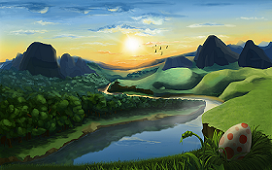
\includegraphics[width=0.7\textwidth]{imgs/sam.png}
	\caption{自20世纪70年代后期以来处理器性能的增长。这个图表绘制了相对于 VAX 11/780 的性能曲线,
            测试数据由SPEC 基准测试测得(见1.8节)。在20世纪80年代中期之前,处理器性能的增长主
            要由技术驱动,平均大约每年增长25\%。在此之后的年增长速度为大约52\%,这一高速增长应当
            归功于更高级的体系结构和组织思想。这样持续发展到2003年时,如果一直以25\%的速度增长,
            处理器性能要比实际性能低25倍。2003年之后,功耗和可用指令级并行的限制减慢了单核处理
            器性能的增长速度,年增长速度不超过22\%,到2010年,如果仍然保持每年52\%的增长速度,
            处理器性能要比实际性能高出大约5倍。(从2007年起,单个芯片上的核心数目每年都在增加,
            最快速的SPEC性能测试已经启用了自动并行,所以很难再测试单核处理器的速率。这些结果仅
            限于单套接字系统,以降低自动并行造成的影响。)图1-4给出了时钟速率在上述三个时期的增长
            速度。由于 SPEC这些年也发生了变化,所以在评估新机器的性能时,对测试数据进行了換算,
            换算因数与两种不同SPEC版本(比如SPEC89、SPEC92、SPEC95、SPEC2000和 SPEC2006)的
            性能有关}
\end{figure}

硬件方面的上述创新导致了计算机设计的复兴,既强调体系结构方面的创新,也重视技术
改进的高效运用。实际增长速度中已经包含了这两方面的因素,所以到2003年,高性能微处理
器大约要比仅依靠技术改进(包含电路设计的改进)快7.5倍;实际年增长速度为52\%,仅依
靠技术改进的年增长速度为35\%。

这一硬件复兴还有第四个影响,那就是对软件开发的影响。自 1978年以来,硬件性能提高
了25 000倍(见图1-1),这样就允许今天的程序员以性能换取生产效率。今天,绝大多数的编
程是使用诸如Java 和\verb|C#|之类的托管编程语言来完成的,代替了以提高性能为目的的C语言和
C++语言。此外,Python 和Ruby 之类的脚本语言(它们的生产效率可能更高),连同Ruby Rails
之类的编程框架,也正在日益普及。为了保持生产效率并尝试缩小性能差距,采用即时
(Just-In-Time)编译器和跟踪编译(Trace-based Compiling)的解释器正在取代过去的传统编译
器和链接器。软件部署也在发生变化,因特网上使用的“软件即服务”(Software as a Service,
Saas)取代了必须在本地计算机上安装和运行的盒装光盘套装(shink-wrapped)软件。

应用程序的本质也在变化。语言、音效、图像、视频正在变得愈加重要,响应时间对于提
供良好的用户体验非常关键,使其保持在可预测范围之内也同样变得愈加重要。Google Goggles
就是一个激动人心的例子。当用户拿起手机,把手机上的镜头对准物体时,这个应用程序可以
通过因特网将图像无线传送到一个仓库级计算机(warechouse-scale computer)上,这个计算机
会识别物体,告诉用户它的一些有趣信息。它可以将物体上的文字翻译为另一种语言;读取书
籍封面上的条码,告诉用户这本书在网上是否有售,价格多少;或者,如果用户播动镜头,拍
摄周围的全景,它还会告诉用户附近有什么商店以及它们的网站、电话号码和方位。

遗憾的是,图1-1还表明这一长达17年的硬件复兴结束了。从2003年开始,由于风冷芯
片最大功耗和无法有效地开发更多指令级并行这两大李生瓶颈,单处理器的性能提高速度下降
到每年不足22\%。事实上,Intel 在2004年取消了自己的高性能单核处理器项目,转而和其他公
司一起宣布:为了获得更高性能的处理器,应当提高一个芯片上集成的核心数目,而不是加快
单核处理器的速度。

这是一个标志着历史性转折的里程碑信号,处理器性能的提高从单纯依赖指令级并行(ILP)
转向数据级并行(DLP)和线程级并行(TLP),ILP是本书前三个版本的重点,第4版开始
重点介绍 DLP 和 TLP,第5版进一步加以扩展。这一版还增加了仓库级计算机和请求级井行
(RLP)的内容。编译器和硬件都是隐式开发IP的,不会引起程序员的注意,而DLP、TLP 和
RLP则是显式并行的,需要调整应用程序的结构才能开发显式并行。在某些情况下,这一调整
比较容易,但在大多数情况下,它会成为程序员的主要新增负担。

本书主要讨论使上世纪飞速增长成为可能的体系结构思想和相关的编译器改进、这些急剧
变化的原因,以及21世纪体系结构思想、编译器和解释器面对的挑战和一些富有前景的方法。
本书的核心内容是一种量化的计算机设计与分析方法,所采用的工具是对程序的经验观察、试
验和模拟。本书中就反映了这种计算机设计风格与方法。本章的目的是为后续各章及附录奠定
量化基础。

编写本书的目的不只是为了解释这种设计风格,还希望激励读者为这一进程作出贡献。这
种量化方法对过去的隐式并行计算机是有效的,我们相信这种方法对未来的显式并行计算机也
同样有效。

\section{计算机的分类}
由于上述变化,我们在新世纪里看待计算、计算应用程序和计算机市场的观点也发生了巨
大变化。自个人计算机诞生以来,我们还没有见到过计算机在外观和操作方式上发生如此之大
的变化。计算机使用方式的变化推动形成了种不同的计算市场,每一种都有自己不同的应用、
需求和计算技术。表1-1总结了主流计算环境及其重要特征。
\begin{table}[]
    % \tiny
    \scriptsize
    \centering
    \begin{tabular}{C{0.09\textwidth}|C{0.15\textwidth}|C{0.15\textwidth}|C{0.15\textwidth}|C{0.15\textwidth}|C{0.15\textwidth}}
        \hline
        特征    & 个人移动设备(PMD)    & 台式机   & 服务器     & 集群/仓库级计算机   & 嵌入式     \\ \hline
        系統价格  & 100$\sim$1000美元     & 300$\sim$2500 美元     & 5000$\sim$10000000美元 & 100000$\sim$200000000美元 & 10$\sim$100000美元   \\ \hline
        微处理器价格    & 10 $\sim$100美元    & 50 $\sim$500美元    & 200 $\sim$2000美元     & 50 $\sim$250美元     & 0.01$\sim$100美元   \\ \hline
        关键的系统设计问题 & 成本,能耗,媒体性能,响应率 & 性价比,能耗,图形性能 & 吞吐量,可用性可扩展性,能耗      & 性价比,吞吐量,能耗均衡性  & 价格,能耗,应用的特有性能 \\ \hline
    \end{tabular}
    \caption{*2010年的销售量包括大约18化个PMD(90\%为手机)、3.5亿个台式PC和2000万个服务器。嵌入或处理器的总销
        售量接近190亿。2010年共交付了61亿个基于 ARM拉术的芯片。注意服务器和嵌入器系純的系統价格跨度极大,
        包含了从USB 密钥到网络路由器在内的各种设备。对于服务器,这一变化范国主要是因汋需要超大規模多处理器系
        统来完成高端事务处理。}
\end{table}

\subsection{个人移动设备}
个人移动设备(PMD)是指一类带有多媒体用户界面的无线设备,比如手机、平板电脑
等。由于整个产品的零售价格为数百美元,所以成本成为一个关键因素。尽管经常会因为使用
电池而需要强调能效,但由于需要使用相对便宜的外壳(由塑料或陶瓷制成),而且缺少冷却风
扇,所以也限制了总功耗。我们将在1.5节更详细地研究能耗和功率。PMD上的应用程序经常
是基于 Web 应用、面向媒体的,比如上面提到的Google Goggles。能耗与尺寸要求决定了要采
用闪存而不是磁盘来作为存储方式(第2章)。

响应性能和可预测性能是多媒体应用程序的关键特性。实时性能需求是指应用程序的一个
程序段有一个确定的最大执行时间。例如,在 PMID上播放一段视频时,由于处理器必须在短
时间内接收和处理下一个视频帧,所以对每个视频帧的处理时间是有限的。某些应用程序中还
有一个更具体的需求:当超出某一最大时间时,会限制一项特定任务的平均时间和实例数目。
如果仅仅是偶尔违反一个事件的时间约束条件(而非过多地发生这种情况),就可以采用有时被
称为软实时的方法。实时性能往往严重依赖于具体的应用程序。

许多 PMD 应用程序中还有其他一些关键特性:需要将存储器占用减至最少,需要高效利
用能量。电池容量和散热问题都需要提高能耗效率。存储器可能在系统成本中占有很大的比例,
在这种情况下,存储器优化是非常重要的。由于应用程序已经决定了数据规模,所以重视存储
器用量其实就是要重视代码规模。

\subsection{桌面计算}
以资金而论,一级市场(可能仍然是最大的市场)是桌面计算市场。桌面计算覆盖了从低
端到高端的整个产品范围,既有售价不到300美元的低端上网本,也有售价可能达2500美元的
高端高配工作站。从2008年开始,每年生产的桌面计算机中有一半以上是由电池供电的笔记本
计算机。

在整个价格与性能范围内,桌面计算机市场都有优化性价比的趋势。系统的性能(主要以
计算性能和图形性能来衡量)和价格对这个市场中的客户来说是最重要的,因此对计算机架构
师也是最重要的。结果,最新、最高性能的微处理器和低成本微处理器经常首先出现
桌面系统中。(1.6节讨论了影响计算机成本的问题。)

尽管以Web 为中心的互动应用日益增多,为性能评估带来了新的挑战,但根据应
测试还是能够较好地刻画桌面计算的特征。

\subsection{服务器}
自20世纪80年代开始转向桌面计算机以来,服务器的角色逐渐变为提供更大规模、更可
靠的文件和计算服务。这些服务器已经代替传统的大型机,成为大规模企业计算的中枢。

对服务器而言,所强调的特征不同于桌面计算机。首先,可用性是至关重要的。(我们将在
1.7节讨论可用性。)考虑一下运行银行 ATM机或者航班订票系统的服务器。由于这些服务器必
须每周7天、每天24小时不间断工作,所以此类服务器系统发生故障时产生的灾难性后果要远
比单个桌面计算机故障严重。表1-2估算了服务器应用程序因宕机所造成的收益成本。

服务器系统的第二个关键特征是可扩展性。服务器系统经常需要扩展,以满足其所支持服
务的增长需求,或者对功能的增长需求。因此,服务器扩展计算容量、内存、存储器和 I/O带
宽的能力极为重要。

最后一个特征,服务器的设计应使其具有很高的吞吐能力。也就是说,服务器的整体性能
(每分钟处理的事务数或者每秒提供的网页数)才是最重要的。尽管对单个请求的响应速度依然
重要,但总体效率和成本效益(由单位时间内能够处理的请求数决定)才是大多数服务器的关
键度量。我们将在1.8节再来讨论如何评估不同计算环境类型的性能问题。

% Please add the following required packages to your document preamble:
% \usepackage{multirow}
\begin{table}[]
    \centering
    \caption{假定有3种不同可用性级别且宕机时间均匀分布,通过分析宕机成本(直接收入损失),给出由于
            系统不可用而带来的成本(四含五入至10万美元)}
    \begin{tabular}{|c|c|ccc|}
    \hline
    \multirow{2}{*}{应用程序} & \multirow{2}{*}{\begin{tabular}[c]{@{}c@{}}每 ⼩ 时 的 宕 机 成 本\\ ( 千 美 元 )\end{tabular}} & \multicolumn{3}{c|}{不同宕机率造成的年度亏换(百万美元)}                                                                                                                                                                                    \\ \cline{3-5} 
                        &                                                                                      & \multicolumn{1}{c|}{\begin{tabular}[c]{@{}c@{}}1\%\\ (87.6小时/年)\end{tabular}} & \multicolumn{1}{c|}{\begin{tabular}[c]{@{}c@{}}0.5\%\\ (43.6小时/年)\end{tabular}} & \begin{tabular}[c]{@{}c@{}}0.\%\\ (8.8小时/年)\end{tabular} \\ \hline
    经纪业务                  & 6450                                                                                 & \multicolumn{1}{c|}{565}                                                      & \multicolumn{1}{c|}{283}                                                        & 56.5                                                     \\ \hline
    信用卡授权                 & 2600                                                                                 & \multicolumn{1}{c|}{228}                                                      & \multicolumn{1}{c|}{114}                                                        & 22.8                                                     \\ \hline
    包裹运输服务                & 150                                                                                  & \multicolumn{1}{c|}{13}                                                       & \multicolumn{1}{c|}{6.6}                                                        & 1.3                                                      \\ \hline
    家庭购物频道                & 113                                                                                  & \multicolumn{1}{c|}{9.9}                                                      & \multicolumn{1}{c|}{4.9}                                                        & 1.0                                                      \\ \hline
    目录销售中心                & 90                                                                                   & \multicolumn{1}{c|}{7.9}                                                      & \multicolumn{1}{c|}{3.9}                                                        & 0.8                                                      \\ \hline
    航空订票中心                & 89                                                                                   & \multicolumn{1}{c|}{7.9}                                                      & \multicolumn{1}{c|}{3.9}                                                        & 0.8                                                      \\ \hline
    手机服务激活                & 41                                                                                   & \multicolumn{1}{c|}{3.6}                                                      & \multicolumn{1}{c|}{1.8}                                                        & 0.4                                                      \\ \hline
    网络在线费用                & 25                                                                                   & \multicolumn{1}{c|}{2.2}                                                      & \multicolumn{1}{c|}{1.1}                                                        & 0.2                                                      \\ \hline
    ATM服务费                & 14                                                                                   & \multicolumn{1}{c|}{1.2}                                                      & \multicolumn{1}{c|}{0.6}                                                        & 0.1                                                      \\ \hline
    \end{tabular}
\end{table}

* 数据来源:Kemiel[2000],由 Contingency Plaming Research 收集、分析。


\subsection{集群/仓库级计算机}
软件即服务(Saas)应用(比如搜索、社交网络、视频分享、多人游戏、在线销售等)的
发展已经推动了一类被称为集群的计算机的发展。集群是指一组桌面计算机或服舒器通过局域
网连接在一起,运转方式类似于一个更大型的计算机。每个节点都运行自己的操作系统,节点
之间使用网络协议进行通信。最大规模的集群称为仓库级计算机(WSC),它们的设计方式使
数万个服务器像一个服务器一样运行。第6章详细介绍了这类超大型计算机。

WSC是如此之大,因而性价比和功耗非常关键。第6 章将解释一一个价值9000万美元的仓
库级计算机,其成本中有80\%与计算机内部的功耗和冷却技术有关。这些计算机本身和网络设
备另外需要7000万美元,每隔几年就必须更换一次。在购买这样大规模的计算设备时,一定
要非常精明,因为性价比提高10\%就意味着可以节省700万美元(7000万美元的10\%)。

WSC与服务器的相通之处在于它们都非常看重可用性。例如,Amazon.com 在2010年第四
季度的销售额为130亿美元。一个季度大约有2200个小时,每小时的平均收入差不多是600万
美元。在圣诞节购物的高峰时间,潜在损失可能要多出许多倍。第6章将会解释,WSC与服务
器的区别在于,WSC以很多廉价组件为构建模块,依靠软件层来捕获和隔离在这一级别进行计
算时发生的许多故障。注意,WSC的可扩展性是由连接这些计算机的局域网实现的,而不是像
服务器那样,通过集成计算机硬件来实现。

超级计算机与 WSC的相通之处在于它们都非常昂贵,需要花费数千万美元,但超级计算
机的不同之处在于它强调浮点性能,会运行大型的、通信密集的批程序,这些程序可能会一次
运行几个星期。这种紧耦合性决定了超级计算级要使用非常快速的内部网络。而WSC则不同,
它重视互动应用程序、大规模存储、可靠性和很高的因特网带宽。

\subsection{嵌入式计算机}
嵌人式计算机在日用电器中随处可见。微波炉、洗衣机、大多数打印机、大多数网络交换
机和所有汽车中都有简单的嵌入式微处理器。

PMID 中的处理器经常被看作是嵌入式计算机,但我们仍然把它们看作一个不同类别,这是
因为 PMD 是一些可以运行外部开发软件的平台,它们与桌面计算机有许多共同特征。其他嵌
入式设备在硬件和软件复杂性方面都有很大的限制。我们以能否运行第三方软件作为区分嵌人
式和非嵌入式计算机的分界线。

嵌入式计算机的处理能力和成本差别最大。它们既包括只需要0.1美元的8位和16位处理
器,也有可以每秒执行1亿条指令、价格低于5美元的32位微处理器,还有用于网络交换机的
高端处理器,它们的售价高达100美元,每秒可以执行数十亿条指令。尽管嵌人式计算市场中
的计算能力相差很大,但价格仍然是此类计算机设计的关键因素。性能要求当然是的确存在的,
但主要目标通常是以最低价格满足性能需要,而不是以更高的价格来获得更高的性能。

本书的大多数内容适用于嵌入式处理器的设计、使用和性能,无论是现成的微处理器,还
是与其他专用硬件组装在一起的微处理器核心,都是适用的。实际上,本书第3版还包含了一
些嵌人式计算示例,用来演示每章的思想。

遗憾的是,大多数读者对第3版中的示例感到不满意,这是因为计算机的量化设计与评估
需要数据来推动,而嵌人计算领域的相关数据还不够充足(参见1.8 节中EEMBC的挑战)。因
此,我们现在只给出定性描述,这种方式与本书其余部分不是特别一致。有鉴于此,在上一版
和这一版中,我们将嵌入计算机的相关材料合并到附录E中。我们认为把它们放在一个单独的
附录中,既便于在正文中流畅地表达思想,又可以让读者了解这些不同需求是如何影响嵌人式
计算的。

\subsection{并行度与并行体系结构的分类}
在所有4个计算机类别中,多种级别的并行度现在已经成为计算机设计的推动力量,而能
耗和成本则是主要约束条件。应用程序中主要有以下两种并行。

\begin{enumerate}
    \item \textbf{数据级并行(DLP)},它的出现是因为可以同时操作许多数据项。
    \item \textbf{任务级并行(TLP)},它的出现是因为创建了一些能够单独处理但大量采用并行方式执
    行的工作任务。
\end{enumerate}

计算机硬件又以如下4种主要方式来开发这两种类型的应用并行。

\begin{enumerate}
    \item 指令级并行在编译器的帮助下,利用流水线之类的思想适度开发数据级并行,利用推理
    执行之类的思想以中等水平开发数据级并行。
    \item 向量体系结构和图形处理(GPU)将单条指令并行应用于一个数据集,以开发数据级
    并行。
    \item 线程级并行在一种紧耦合硬件模型中开发数据级并行或任务级并行,这种模型允许在并
    行线程之间进行交互。
    \item 请求级并行在程序员或操作系统指定的大量去耦合任务之间开发并行。
\end{enumerate}

硬件支持数据级并行和任务级并行的这4种方式可以追溯到50年前。Michael Flynn [1966]
在20世纪60年代研究并行计算工作量时,提出了一种简单的分类方式,我们今天仍在使用这
种分类的缩。他研究了多处理器最受约束组件中的指令流及数据流的并行,并据此将所有计
算机分为以下4类。

\begin{enumerate}
    \item \textbf{单指令流、单数据流(SISD)}:这个类别是单处理器。程序员把它看作标准的顺序计算
    机,但可以利用指令级并行。第3章介绍了采用 ILP技术(比如超标量和推理执行)的SISD体
    系结构。
    \item \textbf{单指令流、多数据流(SIMD)}:同一指令由多个使用不同数据流的处理器执行。SIMD
    计算机开发数据级并行,对多个数据项并行执行相同操作。每个处理器都有自己的数据存储器
    (也就是 SIMD 中的 MID),但只有一个指令存储器和控制处理器,用来提取和分派指令。第4
    章介绍 DLP和3种开发 DLP的不同体系结构:向量体系结构、标准指令集的多媒体扩展、GPU。
    \item \textbf{多指令流、单数据流(MIISD}):到目前为止,还没有这种类型的商用多处理器,但包含
    这种类型之后,这种简单的分类方式变得更完整。
    \item \textbf{多指令流、多数据流(MIMID}):每个处理器都提取自己的指令,对自己的数据进行操
    作,它针对的是任务级并行。一般来说,MIIMD 要比 SIMD更灵活,所以适用性也更强,但它
    要比 SIMD更贵一些。例如,MIMD 计算还能开发数据级并行,当然,其开销可能要比SIMD
    处理器高一些。这种开销是指粒度大小要足够大,以便高效地开发并行度。第5 章介绍紧耦合
    MIMD 体系结构,由于多个互相协作的线程是并行操作的,所以它开发了线程级井行。第6章
    介绍开发请求级并行的松耦合 MIMD 体系结构(具体来说,就是集群和仓库级计算器),在这
    种情况下,可以很自然地并行执行许多独立任务,几乎不需要通信和同步。
\end{enumerate}

这种分类模型很粗略,许多并行处理器是 SISD、SIMD 和 MIMD 的混合类型。不过,我们
可以用它为本书将要介绍的计算机设计空间设定一个框架。

\section{计算机体系结构的定义}

计算机设计人员面对的是一个非常复杂的任务:判断哪些属性对于种新计算机来说是至
关重要的,然后在设计这种计算机时使其性能和能耗效益达到最佳,同时还要满足成本、功耗
和可用性约束条件。这项任务包括许多方面:指令集设计、功能组织、逻辑设计、实现方式。
实现方式可能包括集成电路设计、包装、电池和冷却。为使设计方案达到最优效果,设计人员
需要熟悉从编译器、操作系统到逻辑设计与包装等广泛技术。

几年前,计算机体系结构一词通常仅包括指令集设计。计算机设计的其他方面称为实现,
言下之意通常就是实现方式不太重要,或者说没有什么挑战性。

我们认为这种观点是错误的。架构师的工作远不止指令集设计一项,在项目其他方面遇到
的技术障碍很可能比指令集设计中遇到的障碍更具挑战性。在介绍计算机架构师的更多挑战之
前,先来快速回顾一下指令集体系结构。

\subsection{指令集体系结构:计算机体系结构的近距离审视}
我们在本书中用指令集体系结构(ISA)一词来指代程序员可以看到的实际指令集。ISA的
作用相当于区分软件和硬件的界限。在下面对ISA 的快速回顾中,将使用80x86、ARM 和 MIPS
的例子从7个方面来介绍ISA。附录A和附录K更详细地介绍了这3种ISA。

\begin{enumerate}
    \item ISA分类。现今几乎所有的ISA 都划分到通用寄存器体系结构中,在这种体系结构中,
    操作数或者是寄存器,或者是存储器地址。80x86有16个通用寄存器和16个通常存入浮点数据
    的寄存器,而 MIPS 则有32个通用寄存器和32个浮点寄存器(见表1-3)。这一类别有两种
    主流版本,一种是寄存器-存储器ISA,比如80x86,可以在许多措令中访问存储器;另一种
    是载入-存储ISA,比如ARM 和MIPS,它们只能用载人或存储指令来访问存储器。所有最新
    ISA 都采用载入-存储版本。
    \item 存储器寻址。几乎所有桌面计算机和服务器计算机(包括80x86、ARM 和 MIPS)都使
    用字节寻址来访问存储器操作数。有些体系结构(像 ARM和 MIPS)要求操作对象必须是对齐
    的。一个大小为s的对象,其字节地址为A,如果Amods=0,则对这个对象的访问是对齐的。
    80x86(见附录图 A-2)不需要对齐,但如果操作数是对齐的,访问速度通常会更快一些。
    \item 寻址模式。除了指定寄存器和常量操作数之外,寻址模式还指定了一个存储器对象的地
    址。MIPS 寻址模式为:寄存器(寻址)、立即数(寻址)和位移量(寻址)。立即数寻址用于常
    数寻址,在位移量寻址模式中,将一个固定偏移量加到寄存器,得出存储器地址。80x86 支持
    上述3种模式,再加上位移量的3种变化形式,即:无寄存器(绝对数)、两个寄存器(用位移
    量进行基址寻址)、两个寄存器,其中一个寄存器的内容乘以操作数的字节大小——用比例索引
    和位移量进行变址寻址。它与上述3种寻址方式类似,只是要减去位移量字段,加上寄存器间
    接寻址、基址寻址和变址寻址。ARM 拥有3种 MIIPS 寻址模式再加上相对 PC(程序计数器)
    的寻址方式、两个寄存器之和,还有一种方式也是两个寄存器之和,但其中一个寄存器的内容
    要乘以操作数的字节大小。它还有自动递增寻址和自动递减寻址:计算得到的地址会被放在用
    于构造该地址的一个寄存器中,替代其中的内容。
    \item 操作数的类型和大小。和大多数ISA类似,80x86、ARM和 MIPS 支持的操作数大小为
    8位(ASCII字符)、16位(Unicode 字符或半个字)、32位(整数或字)、64位(双学或长整型)
    以及 IEEE 754浮点数,包括32位(单精度)和64位(双精度)。80x86还支持80位浮点(扩
    展双精度)。
    \item 操作指令。常见的操作类别为:数据传输指令、算术逻辑指令、控制指令(下面进行讨
    论)和浮点指令。MIPS 是一种简单的、易于实现流水化的指令集体系结构,它是2011年采用
    RISC体系结构的代表。表1-4总结了 MIPS ISA。80x86 的操作指令集要丰富得多,大得多(参
    见附录K)。
    \item 控制流指令。几乎所有ISA,包括上述三种在内,都支持条件转移、无条件跳转、过程
    调用和返回。所有这三种都使用相对于PC的寻址方式,其中的分支地址由一个地址字段指定,
    该地址将被加到 PC。这三种 ISA 之间有一些微小的区别。MIPS 条件分支(BE、BNE等)检验
    寄存器中的内容,而80x86 和 ARM分支测试条件代码位,这些位是在执行算术/逻辑运算时顺
    带置位的。ARM和 MIPS 过程调用将返回地址放在一个寄存器中,而80x86调用(CALLF)将返
    回地址放在存储器中的一个栈内。
    \item ISA 的编码。有两种基本的编码选择:固定长度和可变长度。所有ARM和 MIPS 指令
    的长度都是32位,从而简化了指令译码。图1-2给出了 MIPS指令格式。80x86编码为可变长
    度,变化范围为1~18个字节。与固定长度的指令相比,可变长度的指令可以占用较少的空间,
    所以为80x86编译的程序通常要小于为 MIIPS 编译的相同程序。注意,上面提到的编码选择会
    影响将指令转换为二进制编码的方式。例如,由于寄存器字段和寻址模式字段可以在一条指令
    中出现许多次,所以寄存器的数目和寻址模式的数目都对指令的大小具有显著影响。(注意,
    ARM 和 MIIPS 后来都进行了扩展,支持长16位的指令,以便缩小程序规模,这两种扩展分别
    叫做 Thurb 或 Thumb-2、MIPS16)
\end{enumerate}

\begin{table}[]
    \centering
    \caption{MIPS寄存暑和使用规范}
    \begin{tabular}{|c|c|c|c|}
    \hline
    名称             & 编号  & 用途         & 在调用之间是否保留 \\ \hline
    \verb|$zero|    & 0     & 常量值O                   & 不可用 \\ \hline
    \verb|$at|      & 1     & 为汇编程序保存的临时寄存器    & 否 \\ \hline
    \verb|$v0-$v1|  & 2~3   & 函数返回值和表达式计算结果的值 & 否 \\ \hline
    \verb|$a0-$a3|  & 4~7   & 实参                      & 否 \\ \hline
    \verb|$t0-$t7|  & 8~15  & 临时变量                   & 否 \\ \hline
    \verb|$s0-$s7|  & 16~23 & 已保存的临时变量            & 是 \\ \hline
    \verb|$t8-$t9|  & 24~25 & 临时变量                   & 否 \\ \hline
    \verb|$K0-$k1|  & 26~27 & 沟操作系統内核保留          & 否 \\ \hline
    \verb|$gp|      & 28    & 全局指针                  & 是 \\ \hline
    \verb|$sp|      & 29    & 栈指针                    & 是 \\ \hline
    \verb|$fp|      & 30    & 帧指针                    & 是 \\ \hline
    \verb|$ra|      & 31    & 返回地址                  & 是 \\ \hline
    \end{tabular}
\end{table}
\begin{verbatim}
    *除了32个通用寄存器(RO-R31)之外,MIPS 还有32 个浮,点寄存器(FO-F31),可以保存一个32 位单精度教或一
    个64位双精度数。
\end{verbatim}

\begin{verbatim}
    表1-4 MIPS64 中的部分指令
    指令类型/操作码
    数据传输
    LB、LBU、SB
    LH、LHU、SH
    LALHUSW
    LD、SD
    L.S.L.D、S.S、S.D
    MFCO、MTCO
    HOV.S、MDV.D
    MFC1、MTCL
    算术/逻辑
    DADD、DADDI、DADOU、DADDTU
    DSUB、DSUBU
    CMUL、DMULU、DOIV、 DDIVU、MADD
    AND、ANDI
    OR、ORI、XOR、XORI
    LUI
    DSLL、 DSRL、DSRA、DSLLY、DSRLV、
    DSRAV
    SLT、SLTI、SLTU.SLTIU
    控制
    BEQZ、BNEZ
    BEQ、BNE
    BCIT、BCIF
    MOVN、MOVZ
    J、JR
    指令含义
    在奇存册和存储器之间,或者在整数和FP或特珠寄存器之间移动数据:唯一的存
    储器寻址樸式是16位位移量加上GPR的内容
    载入字节、载人无符号字节、存储字节(至/自整数寄存器)
    载人半字、载入无符号半字、存储半字(至/自鳖数寄存器)
    载人字、载人无符号字、存储字(至/自整数寄存器)
    载人双字、存储双字(至/自整数寄存器)
    载人SP浮点、载入DP浮点、存储SP浮点、存储DP浮点
    在GPR与特殊寄存器之间复制数据
    将一个SP或DPFP寄存器复制到另一个FP寄存器
    在FP寄存器与整数寄存器之间复制132位
    对GPR中的整数或逻辑数据进行操作:带符号算术运算溢出时进行陷阱捕获
    加,加立即数(所有立即数为16位),有符号和无符号
    减,有符号和无符号
    乘和除,有符号和无符号,乘-加;所有运算的操作数和结果都是64位数值
    与,和立即数相与
    或,和立即数求或,异或,和立即数求异或
    载入高位立即数:将立即数载人到寄存器的32~47位,然后进行符号扩展
    移位:立即数形式(DS_)和变量形式(DS_V),移位为左逻辑移位、右涩辑移
    位、右算术移位
    若小于操作数则置位、若小于立即数则置位、有符号和无符号
    控制分支和迷转,相对于PC寄存晋或通过寄存器控制
    GPR等于/不等于0时转移、相对于PC+4偏移16位偏移量
    GPR相等/不相等时转移、相对于PC+4转移16位偏移
    测试FP状态寄存器中的对比位,并转移:相对于PC+4转移16位偏移量
    如果第三个GPR为负数/零,则将第一个GPR复制到第二个GPR
    眺转至与PC+4偏移26位偏移量的位置(J)、眺转至寄存器中的目标位置(JR)
    (续)
    指令类型/操作码
    指令含义
    JAL、JALR
    眺转和链接:将PC+4保存在R31中,目标为相对于PC(JAL)或寄存器(JALR)
    TRAP
    转移到操作系统的一个向量地址
    ERET
    从异常中返回用户代码,恢复用户模式
    浮点
    对DP和SP格式执行FP操作
    AD0.D、ADD.S、ADD.PS
    DP、SP数相加,一对SP数相加
    SUB.D、SUB.S.SUB.PS
    DP、SP数相减,一对SP数相减
    MUL.D、MUL.S、MUL.PS
    DP、SP浮点数相乘,一对SP数相乘
    MADD.D、MADD.S、MADD.PS
    DP、SP浮点数相乘加,一对SP數相乘加
    DIV.D、DIV.S、DIV.PS
    DP、SP浮点数相除,一对SP数相除
    CVT!-
    转換指令:CVT.X.y从类型x转換为类型Y,其中x和 为L(64位整数),W(32位整
    数),D(DP)或S(SP)。两个操作数都是FRP
    C.
    _.D、C._.S
    DP和SP对比:“_”=LT,GT,LE,GE,EQ,NE,在FP状态寄存器中置位
    *SP-单精度、DP-双精度附录A给出了有关 MIPS64的更多详细信您。对数据而言,最高有效位编号为0,最低有效
    位为 63。
\end{verbatim}

除了ISA设计方面的挑战之外,如果指令集之间的区别很小,如果存在不同的应用领域,
那计算机架构师面对的其他挑战将更加严重。因此,从本书上一版开始,除了这里给出的快速
回顾之外,还在附录中提供了大量有关指令集的材料(参见附录A和网站上的附录K)。

本书以 MIPS64 的于集作为ISA 的例子,是因为它既是网络领域的主导ISA,又是前面提
到的 RISC 体系结构的出色示例,ARM (Advanced RISC Machine,高级 RISC 机器)是 RISC
体系结构的最流行示例。2010年出产的芯片中有61 亿个采用了 ARM处理器,与采用80x86处
理器的芯片相比,大约是其20倍。

MIPS64 指令集体系结构格式。所有指令的长度都是32位。R格式用于整数寄存器至寄存器操作,
比如 DADDU、DSUBU等。格式1用于数据传送、分支和立即数指令,比如L.D、SD、BEQZ 和
DADDIo格式J用于跳转指令,FR格式用于浮点操作,FI格式用于浮点分支

\subsection{真正的计算机体系结构:设计满足目标和功能需求的组成和硬件}
计算机的实现包括两个方面:组成和硬件。组成一词包含了计算机设计的高阶内容,比如
存储器系统,存储器互连,设计内部处理器或CPU(中央处理器——算术、逻辑、分支和数据
输送功能都在这里实现)。有时也使用微体系结构一词来代替“组成”。例如,AMD Opteron 和
Intel Core i7 是两个指令集体系结构相同但组成不同的处理器。这两种处理器都实现x86 指令集,
但它们的流水线和缓存组成有很大不同。

由于单个微处理器上开始采用多个处理器,所以人们开始使用核心一词来称呼处理器。人
们一般不说“多处理器微处理器”,而是使用“多核”。由于现今几乎所有芯片都有多个处理器,
所以人们不怎么使用中央处理器(或CPU)一词了。

硬件是指一个计算机的具体实现,包括计算机的详尽逻辑设计和封装技术。同一系列的计
算机通常具有相同的指令集体系结构和几乎相同的组成,但在具体硬件实现方面有所不同。例
如,Intel Core i7(见第3章)和 Intel Xeon 7560(见第5章)基本相同,但提供不同的时钟速
率和不同的存储器系统,Xeon 7560更适用于服务器计算机。

在本书中,体系结构涵盖了计算机设计的所有三个方面:指令集体系结构、组成或微体系
结构、硬件。

计算机架构师设计的计算机必须满足功能需求,并达到价格、功耗、性能和可用性指标。
表1-5总结了在设计新计算机时要考虑的要求。通常,架构师还必须判断有什么样的功能要求,
其中哪一项可能是主要任务。需求可能是由市场驱动的特定功能。应用软件决定了计算机的使
用方式,从而经常会推动特定功能需求的选择。如果存在大量为一特定指令集体系结构设计的
软件,那架构师可能会决定:新计算机应当实现这种已有指令集。如果某类应用程序拥有庞大
的市场,那可能会鼓励设计人员整合一些需求,使计算机在这一市场上具有更强的竞争力。后
面章节将深入研究大量此类需求和功能。
\begin{table}[]
    % \tiny
    % \small
    \scriptsize
    \centering
    \caption{架构师面对的一些最重要功能需求汇总}
    \begin{tabular}{C{0.15\textwidth}C{0.7\textwidth}}
    \hline
    \textbf{功能需求}         & \textbf{应当具备或支持的典型特性} \\ \hline
    \textbf{应用领域}         & \textbf{计算机的目标} \\
    个人移动设备         & 一系列任务的实时性能,包括图形、视频和音频的交互性能,能效(第2、3、4、5章,附录A) \\
    通用桌面计算机         & 一系列任务的均衡性能,包括图形、视频和音频的交互性能:能效(第2、3、4、5章,附录A) \\
    服务器         & 支持数据库和事务处理,可靠性和可用性的增强,支持可伸缩性(第2、5章,附录A.D、F) \\
    集群/仓库级计算机         & 许多独立任务的吞吐量性能,存储器的纠错功能,能耗均衡(第2、6章,附录F) \\
    嵌入式计算         & 通常需要对图形或视频提供特支持(或者其他专用扩展),可能需要功耗限制和电源控制,实时約束(第2、3、5章,附录A、E) \\ \hline

    \textbf{软件兼容级别}         & \textbf{决定计算机的现有软件数目} \\
    在编程语言级别         & 对设计人员来说最为灵活,需要新编译器(第3、5章,附录A) \\
    目标代码或二进制代码兼容性         & 指令集体系结构完全确定(几乎没有灵活性),但不需要在软件或端口程序中进行投人(附录A) \\ \hline

    \textbf{操作系统需求}         & \textbf{支持选定OS所需要的特性(第2章、附录B)} \\
    地址空间的大小         & 非常重要的特性(第2章),可能会限制应用 \\
    存储器管理         & 为现在操作系统所必需,可能进行分页或分段(第2章) \\
    保护         & 不同的操作系統和应用需要:分页或分段,虚拟机(第2章) \\ \hline

    \textbf{标准}         & \textbf{市场可能要求特定的标准} \\
    浮点         & 格式和算法:IEEE 754标准(附录J),用于图形处理或信号处理的特殊算法 \\
    I/O接口         & 对于I/O设备:申行ATA,串行连接SCSI、PCI Express(附录D、F) \\
    操作系统         & UNIX, Windows、Linux,CISCO IOS \\
    网络         & 支持不同网络:以太网、Infiniband(附录F) \\
    编程语言         & 语言(ANSIC、C++、Java、Fortran)影响指令集(附录A) \\ \hline
    \end{tabular}
\end{table}
\begin{verbatim}
    *左列描述需求的类别,右列给出特定示例,还包含讨论相应主题的章节和附录。
\end{verbatim}
架构师还必须了解技术和计算机应用这两方面的重要趋势,因为这些趋势不仅会影响未来
的成本,还会影响到体系结构的寿命。
\section{技术趋势}
一种指令集体系结构要取得成功,它的设计必须能够适应计算机技术的快速变化。毕竟,
一种成功的新指令集体系结构可能要持续几十年——例如,TBM 大型机的核心已经使用了将近
50年。一种成功的计算机可能会因为技术变革而延长寿命,架构师必须提前为此类技术变革做
出应对计划。

要为计算机的发展作长远计划,设计人员必须了解实现技术的快速变化。以下5种实现技
术是现代计算机实现不可或缺的,它们都在发生急剧的变化。

\begin{itemize}
    \item 集成电路逻辑技术。晶体管密度每年大约增加35\%,差不多每四年时间翻两番。晶片大
    小的增长速度要慢一些,也比较难以预测,每年在10\%到20\%之间。两者综合起来,一
    个芯片上的晶体管数目每年大约增长40\%~55\%,或者说每18~24个月翻番。这就是人
    们熟悉的摩尔定律。器件的增长速度要慢一些,下面将进行讨论。
    \item 半导体 DRAM(动态随机访问存储器)。由于大多数 DRAM芯片主要是以 DIMM 模块形
    式交付的,所以很难跟踪芯片容量,因为DRAM 制造商通常会同时提供几种容量产品,
    以与 DIMM 容量相匹配。最近几年来,单个 DRAM芯片的容量每年增加大约25\%~40\%,
    大约每2~3年翻一番。这一技术是主存储器的基础,我们将在第2章详细讨论。注意,
    从表1-6可以看出,这一增长速度一直在随着本书的反复再版而下降。由于高效制造更
    小型 DRAM 单元的难度持续增大,人们甚至在担心,在5~7年内会不会停止增长[Kim
    2005]。第2章提到了其他几种技术,可以在 DRAM 碰到容量壁垒时取代它。
    \item 半导体闪存(电可擦编程只读存储器)。这种永久性半导体存储器是 PMD中的标准存储
    器件,普及率的迅速提高刺激了其容量的快速增加。最近几年,单个闪存芯片的容量以
    每年大约50\%~60\%的速度增长,大约每两年翻一番。2011年,每比特的闪存价格大约
    是DRAM价格的1/15~1/20。第2章将详细探讨闪存。
    \item 磁盘技术。在1990年之前,磁盘密度每年提高大约30\%,3年翻一番。之后每年增长60%,
    1996年的增速为100\%。从2004年开始,已经回落到大约40\%,每3年翻一番。每比特
    的磁盘价格大约是闪存价格的1/15~1/25。由于DRAM 的增长速度缓慢,所以每比特的
    磁盘价格现在大约是 DRAM的1/300~1/500。这一技术是服务器和仓库级存储的核心技
    术,附录D中详细讨论了这些变化趋势。
    \item 网络技术。网络性能取决于交换机性能和传输系统的性能。附录F中详述了网络技术的
    趋势。
\end{itemize}

\begin{table}[]
    % \tiny
    % \small
    % \scriptsize
    \centering
    \caption{DRAM 容量增长速度随时间的变化}
    \begin{tabular}{cccc}
    \hline
    \textbf{CA:AQA版本}         & \textbf{年份} & \textbf{DRAM增长速率(年)} & \textbf{DRAM容量的增长特征} \\ \hline
    1 & 1990 & \verb|60%|       & 每\verb|3|年翻两番 \\
    2 & 1996 & \verb|60%|       & 每\verb|3|年翻两番 \\
    3 & 2003 & \verb|40%~60%|   & 每\verb|3~4|年翻两番 \\
    4 & 2007 & \verb|40%|       & 每\verb|2|年翻一番 \\
    5 & 2011 & \verb|20%~0%|    & 毎\verb|2~4|年翻一番 \\ \hline
    \end{tabular}
\end{table}
\begin{verbatim}
*前两个版本甚至将这一速率称为 DRAM 增长经验定律,因 从1977年的 16Kbi DRAM到1996年的 64MIbit DRAM,
始终都是以这一速率增长的。由于大容量三维 DRAM 单元的制造难度,有人开始担心 DRAM容量在5-7年之内是
否会究全停止增长[Kitm 2005]。
\end{verbatim}

这些快速发展的技术左右着计算机设计的命运,由于计算速度的激增和技术的迅猛发展,
一种计算机设计的生存周期可能只有3~5年。DRAM、闪存和磁盘等关键技术的发展如此之快,
设计人员必须为应对这些变化作好打算。事实上,设计人员在设计时经常要考虑到下一代技术,
因为他们知道,当一件产品开始大量交付时,下一代技术可能是最具成本效益的,或者可能拥
有性能优势。一般来说,成本的下降速度与密度的增长速度大体相当。

尽管技术进步是连续性的,但只有当技术积累到一定程度,为新功能的出现作好准备时,
才会产生跳跃性的、不连续的影响。比如,当MOS 技术在20世纪80年代早期发展到可以在单
片芯片上集成25000 到50000个晶体管时,才使单片32位微处理器的制造成为可能。到20世
纪80年代后期,一级缓存可以出现在一个芯片上。通过消除处理器内部以及处理器与缓存之间
的芯片交叉,使成本效率和能耗效率的大幅提高成为可能。在技术发展到一定程度之前,这种
设计就无法付诸实现。随着多核微处理器的出现以及每一代核心数目的增加,甚至服务器计算
机也开始追求将所有处理器放在一片芯片上。这类技术门槛绝非罕见,对众多设计决策都有着
重要影响。

\subsection{性能趋势:带宽胜过延迟}
在1.8节将会看到,带宽和吞吐量是指在给定时间内完成的总工作量,比如在进行磁盘
传送时每秒完成的MIB 数。与之相对,延迟或响应时间是指一个事件从开始到完成所经历的
时间,比如一次磁盘访问需要的毫秒数。图1-3绘制了微处理器、存储器、网络和磁盘等各项
技术在产生里程碑式进步时,带宽与延迟的相对改进曲线。表1-7更详细地描述了这些示例和
里程碑。

表1-7中各个带宽与延迟里程碑相对于第一个里程碑的双对数曲线。注意,延迟的改进为6~8倍,
而带宽的改进为300~25000倍。更新自 Patterson[2004]

\begin{verbatim}
    表1-7 微处理、存储器、网络和磁盘在过去20~40年里的性能里程碑
    16位地址 32 位 地
    5级流水线、
    微处理器
    /总线、微
    址/总线、
    片上1&D缓
    2路超标基、
    乱序3路超
    乱序超流 多核000 4
    编码
    微编码
    64位总线
    标盘
    水线、片上
    路片上L3缓
    存、FPU
    L2缓存
    存、Turbo
    产品
    Intel
    Intel
    Intel 80486
    Intel Pentium
    Intel
    Intel
    Intel Core i7
    80286
    80386
    Peatium Pro
    Pentium 4
    年份
    1982
    1985
    1989
    1993
    1997
    2001
    2010
    晶片大小(平方
    47
    43
    90
    308
    217
    240
    毫米)
    晶体管数
    处理器数/芯片
    管脚
    延迟(时钟周期)
    总线宽度(位)
    134 000
    1
    68
    6
    16
    275 000
    1
    132
    5
    1200 000
    1
    168
    5
    32
    3 100000
    1
    273
    5
    64
    5500000
    42 000000
    1 170000 000
    1
    387
    10
    1
    423
    22
    64
    4
    1366
    14
    196
    16
    第1章 量化设计 *!
    时钟频率(MHiz)
    带宽 (MIPS)
    延迟(ns)
    存储器模块
    12.5
    2
    320
    DRAM
    模块宽度(位)
    年份
    MbivDRAM芯片
    晶片大小(平方
    16
    1980
    0.06
    35
    毫米)
    管脚/DRAM芯 16
    片
    带宽(MB/s)
    延迟(ns)
    局域网
    16
    6
    313
    分页模式
    DRAM
    16
    1983
    0.25
    45
    16
    —
    25
    25
    200
    快速分页模
    式DRAM
    32
    1986
    1
    70
    18
    66
    132
    76
    快速分页模
    式DRAM
    64
    1993
    16
    130
    20
    200
    600
    50
    同步DRAM
    64
    1997
    64
    170
    54
    1500
    4500
    15
    双数据率
    SDRAM
    64
    2000
    256
    204
    66
    (续)
    3333
    $0 000
    4
    DDR3
    SDRAM
    64
    2010
    2048
    $0
    134
    13
    225
    以太网
    40
    170
    快速
    160
    125
    cbit太网
    267
    640
    75
    62
    1600
    52
    16000
    37
    10Gbit
    100Gbit
    以太网
    以太网
    以太网
    IEBE标准
    年份
    带宽(Mbit/s)
    延迟(us)
    硬盘
    产品
    802.3
    803.34
    802.3ab
    802.3ac
    802.3ba
    1978
    1995
    1999
    2003
    2010
    10
    100
    1000
    10000
    100000
    3000
    500
    340
    190
    100
    3600RPM
    5400 RPM
    7200RPM
    10000RPM
    15 000 RPM
    15 000 RPM
    CDC
    希捷
    希捷
    希捷
    希捷
    希捷
    Wrenl
    94145-36
    ST41600
    ST15150
    ST39102
    ST3734$3
    $T3600057
    年份
    1983
    1990
    1994
    1998
    2003
    2010
    容量(GB)
    0.03
    1.4
    4.3
    9.1
    73.4
    600
    磁盘物理尺寸
    5.25英寸
    5.25英寸
    3.5英寸
    3.5英寸
    3.5英寸
    3.5英寸
    介质直径
    5.25英寸
    5.25英寸
    3.5英寸
    3.0英寸
    2.5英寸
    2.5英寸
    接口
    ST-142
    SCSI
    SCSI
    sCSi
    SCSI
    SAS
    帶宽 (MB/s)
    0.6
    4
    9
    24
    86
    204
    延迟(ms)
    48.3
    17.1
    12.7
    8.8
    5.7
    3.6
\end{verbatim}
*微处理器里程碑是几代IA-32处理醫,从16位慈线、微編码80285到64位总线、多核、乱序执行、超流水线 Core i7。
存储露樸块里程碑包括从 16位宽、纯 DRAM 到64 住宽双教据率第3版同步 DRAM。以太网从 10Mbit/S 发展到
100Gbit/s。磁盘里程碑是 以旋转速魔为标志的,从3600 RPM至15 000 RPM。每种情况都是指最佳带宽,延退就是
假定没有争用时执行简单操作的时间。更新自 Patterson[2004]o

性能是区分微处理器和网络的主要指标,所以它们的进步最大:带宽为10000~25000倍,
延迟为30~80倍。对容量和磁盘来说,容量通常要比性能更重要,所以容量的提高最多,但带
宽发展了300~1200倍,仍然要远远高于延迟的6~8倍。

显然,在这些技术的发展过程中,带宽完胜延迟,而且这一趋势很可能会继续下去。一个
简单的经验法则是:带宽的增长速度至少是延迟改进速度的平方。计算机的设计人员应当制定
相应规划。

\subsection{晶体管性能与连线的发展}
集成电路的制造工艺是用特征尺寸来衡量的,所谓特征尺寸就是一个晶体管或一条连线在
x方向或y方向的最小尺寸。特征尺寸已经从 1971年的10微米下降到2011年的0.032微米;事
实上,我们已经改变了单位,所以2011年的产品工艺被称为“32纳米”,22纳米的芯片也在研
发之中。由于每平方毫米硅片上的晶体管数目是由单个晶体管的表面积大小决定的,所以当特
征尺寸线性下降时,晶体管密度将以平方曲线上升。

不过,晶体管性能的增长就要更复杂了。当特征尺寸缩小时,器件在水平方向以平方关系
缩小,在垂直方向上也会缩小。垂直方向上的缩小需要降低工作电压,以保持晶体管的正常工
作和可靠性。缩放因子的这种组合效果使晶体管性能和工艺特征尺寸之间产生了复杂的相互关
系。大致来说,晶体管性能的提高与特征尺寸的下降成线性关系。

当特征尺寸下降时,晶体管性能以线性提升,而晶体管数目却是以平方曲线增长,这一事
实既是挑战,也是机遇,计算机架构师就是为此而生的!在微处理器发展的早期,借助晶体管
密度的这种快速增长,微处理器迅速从4位发展到8位、16位、32位乃至64位。最近几年,
密度的增长已经足以支持在一个芯片上引入多个处理器,支持更宽的SIMD单元、推理执行和
缓存中的许多创新,在第2、3、4、5章将会讨论这些内容。

尽管晶体管的性能通常会随着特征尺寸的缩小而得到提升,但集成电路中的连线却不会如
此。具体来说,一段连线的信号延迟与其电阻、电容的乘积成正比。当然,当特征尺寸缩小时,
连线会变短,但单位长度的电阻和电容都会变差。这种关系很复杂,这是因为电阻和电容都依
赖于工艺的具体细节、连线的几何形状、连线的负载,甚至取决于与其他结构的邻近程度。偶
尔也会存在一些工艺方面的改进,比如铜的引入,这些改进会一次性地改善连线延迟性能。

一般来说,与晶体管性能相比,连线延迟方面的改进小得可怜,增加了设计人员面临的挑
战。在过去几年里,除了功率耗散方面的限制之外,连线延迟已经成为大型集成电路的主要设
计限制,往往比晶体管开关延迟还要关键。越来越多的时钟周期被消耗在信号在连线上的传播
延迟上,而功率现在扮演的角色甚至比连线延迟还要重要。

\section{集成电路中的功率和能耗趋势}
今天,对于几乎所有类型的计算机来说,功率都是计算机设计人员面对的最大挑战。第一,
必须将功率引入芯片,并进行分配,而现代微处理器仅仅为电源和接地就使用了数以百计的管
脚和多个互连层。第二,功率以热的形式耗散,必须消除。

\subsection{功率和能耗:系统观点}
系统架构师或用户应当如何考虑性能、功率和能耗呢?从系统架构师的角度来看,共有三
个主要关注事项。

第一,一个处理器需要的最大功率是多少?满足这一要求对于确保正确操作非常重要。例
如,如果处理器试图汲取的功率大于电源系统能够提供的功率(也就是试图汲取的电流大于电
源系统能够提供的电流),其结果通常会导致电压下降,而电压下降可能会导致器件无法正常工
作。现代处理器在峰值电流时的功耗变化范围很大,因此提供了电压指数方法,允许处理器减
缓速度,在更大幅度内调𤨣电压。显然,这样会降低性能。

第二,持续功耗是多少?这个度量普遍称为热设计功耗(TDP),这是因为它决定了冷却需
求。TDP 既不是峰值功率(峰值功率通常要高1.5倍),也不是在一个给定计算期间消耗的实际
平均功率(它可能还要更低一些)。在为一个系统设定典型电源型时,其功率通常要大于TDP,
而一个冷却系统通常设计为与 TDP相匹配或大于 TDP。如果不能提供足够的冷却功率,可能会
使处理器中的结点温度超出最大值,导致器件故障,甚至永久损坏。由于最大功率可能超出 TDP
指定的长期平均值(从而使热量和温度上升),所以现代处理器提供了两项功能来帮助管理热量。
第一,当温度接近结点温度上限时,电路降低时钟频率,从而减小功率。如果这一技术不成功,
则启用第二热过载启动装置,以降低芯片的功率。

设计者和用户需要考虑的第三个因素是能耗和能耗效率。回想一下,功率就是单位时间的
能耗:1瓦=1焦/秘。哪个度量更适合对比处理器呢:能耗,还是功率?一般来说,能耗总是要
更好一些,因为它与特定任务以及该项任务所需要的时间结合在一起。具体来说,执行一项工
作负载的能耗等于平均功率乘以此项工作负载的执行时间。

因此,如果我们想知道两种处理器中的哪一个对于某一给定任务更为高效,应当对比执行
该项任务的能耗(而不是对比功率)。例如,处理器A可能比处理器B的平均功耗高20\%,但如
果A执行该任务的时间仅为B所需时间的70\%,它的能耗就是1.2×0.7=0.84,显然要更好一些。

有人可能会说,在一个大型服务器或者云中,由于工作负载经常被认为是无限的,所以考
虑平均功率就足够了,但这是一种误导。如果云中填充的是处理器B,而不是处理器A,那这
个云在消耗相同能量的情况下,所做的工作会更少一些。使用能耗进行对比可以避免这一谬误。
只要我们的工作负载是固定的,那无论是仓库规模的计算机,还是智能手机,在对比处理器时
使用能耗指标总是正确的方法,因为无论是云的电费单还是智能手机的电池寿命,都是由所消
耗的能量决定的。

那功率消耗什么时候才是一种有用的衡量指标呢?它的主要合理用途是作为一一种约束条
件:比如,一个芯片的功率可能被限定为不得超过100瓦。如果工作负载是固定的,那就可以
用它来进行度量,但在这种情况下,它只不过是平均任务能耗这一真正度量的变体。

\subsection{微处理器内部的能耗和功率}

对CMOS芯片来说,传统的主要能耗源是开关晶体管,也称为动态能耗。每个晶体管所需
要的能耗与该晶体管驱动的容性负载与电压平方的乘积成正比:

能耗s盎容性负载×电压2

这个公式的计算结果就是逻辑转变脉冲01-0或1-20 1的能耗。那么一次转換(0 1或1-+0)
的能耗就是:

能耗非 1/2×容性负载 x 电压2

每个晶体管所需要的功率就是一次转换的能耗与转换频率的乘积:

功率猫1/2×容性负载×电压2x开关频率

对于一项固定任务,降低时钟频率可以降低功率,而不会降低能耗。

显然,通过降低电压可以大幅降低动态功率和能耗,所以在20年里,电压已经从5V降低
到 1V 以下。容性负载的大小取决于输出端连接的品体管数目及所用技术,这种技术决定了连
线和晶体管的电容。

例题
现在的一些微处理器设计采用可调电压,电压降低15%可能导致频率下降 15%。
这对动态能耗和动态功率有什么影响?
解答
由于电容值不变,所以能耗变化就是电压平方之比:
-=0.852=0.72
能耗廒
因此,能耗大约降为原能耗的72%。对于功率,需要考虑频率的比值:
功率 =0.72×(开关救率×0.85)=0.61
功率繳
开关频率
缩小到原功率的大约61%。

当我们从一种制造工艺转向另一种工艺时,晶体管的开关次数以及其开关频率的增高强于
负载电容和电压的下降,从而导致功耗和能耗的总体上升。第一代微处理器消耗的功率低于1
瓦,第一代32位微处理器(比如 Intel 80286)消耗大约2瓦,而3.3GHz Intel Core i7 消耗 130
瓦。如果这些热量必须从旁边的一个大约为1.5cm的芯片上消散出去,那实际已经达到了风冷
所能达到的极限。

根据上述公式,如果不能降低电压或提高每个芯片的功率,那可能就要减缓时钟频率的增
长速度。图14表明,实际上从 2003年开始就已经是这种局势了,图1-1中的微处理器都是每
一年度的最佳处理器,它们也无一例外。注意,图 1-4中具有平坦时钟频率曲线的那段时期与
图1-1 中性能改进缓慢的时期相对应。

图1-1中各微处理备时钟频率的增长。从1978年到1986年,时钟频率的年增长速度低于1.5\%,
而性能的年增长速度为25\%。在1986年到2003年性能年增长速度达到52\%的“复兴时期”,时钟
频率飞速增长,几乎达到每年40\%。之后,时钟速率几乎停滞不前,每年的增长速度低于 1\%,
而单处理器性能的年增长速度低于22\%

分配功率、消散热量和防止热区已经变成难度日增的挑战。功率是现在使用品体管的主要
限制,在过去,主要约束体现在原料硅区域。因此,现代微处理器提供了许多技术,试图在时
钟频率和电源电压保持不变的情况下,提高能耗效率。

(1)以逸待劳。今天的大多数微处理器都会关闭非活动模块的时钟,以节省能耗和动态功率。
例如,如果没有正在执行浮点指令,浮点单元的时钟将被禁用。如果一些核心处于空闲状态,
它们的时钟也会被停止。

(2) 动态电压-频率调整(DVFS)。第二种技术直接来自上述公式。个人移动设备、膝上型
电脑、甚至服务都会有一些活跃程度较低的时期,在此期间不需要以最高时钟频率和电压运转。
现代微处理器通常提供几种能够降低功率和能耗的工作时钟频率和工作电压。图1-5绘制了当
工作负载降低时,服务器通过 DVFS 可能节省的功率,三种不同时钟频率为:2.4GHZ、1.8 GHIz
和1GHz。在这两个步骤的每一步中,服务器节省的总功率大约为10\%~15\%。

图1-5
采用 AMD Opteron 微处理器、8 GB DRAM、一个 ATA磁盘的服务节省的能耗。工作频率力
1.8 GHz时,服务器在不降低服务水平的情况下最多只能处理三分之二的工作负载,当工作频率
为1.0GHz时,只能安全地处理三分之一的工作负载(Barroso、Holzle[2009]书中的图5-11)

(3) 针对典型情景的设计。由于 PMD 和膝上型电脑经常空闲,所以内外存储器都提供了
低功率模式,以节省能耗。例如,DRAM具有一系列功率逐渐降低的低功率模式,用于延长 PMD
和膝上型电脑的电池寿命,针对磁盘也提出了一些建议,在空闲时使其采用低转速模式,以节省
功率。遗憾的是,我们不能在这些模式下访问 DRAM 和磁盘,无论访问速度有多低,都必须返
回全速工作模式才能进行读写。前面曾经提到,PC微处理器的设计已经考虑了一种更典型的情
景:在高工作温度下密集使用,这种设计依靠片上温度传感器检测应当在什么时候自动减少活动,
以避免过热。这种“紧急减速”使制造商能够针对一种更典型的情景进行设计,如果运行程序消
耗的功率真的远远超出典型功率,则可以依靠这种安全机制来保证安全。

(4) 超频。Intel 在2008年开始提供 Turbo模式,在这种模式中,芯片可以判定在少数几
个核心上以较高时钟频率短时运行是安全的,直到温度开始上升为止。例如,3.3 GHz Core i7
可以在很短的时间内以3.6GHz的频率运行。实际上,从2008年开始,图1-1 中每一年度最高
性能的微处理器都提供了短时超频功能,超频频率大约比标称时钟频率高10%。在执行单线程
代码时,这些微处理器可以仅留下一个核心,并使其以更高时钟频率运行,而其他所有核心均
被关闭。注意,操作系统可以关闭 Turbo模式,而且在启用时也没有通知,所以程序员可能会
惊奇地发现,他们的程序可能会因为室温而发生性能变化。

尽管通常认为动态功率是 CMOS 中的主要功率耗散源,但由于即使晶体管处于截止状态时
也存在泄漏电流,所以静态功率也正在成为一个重要问题:

功率糖态 电流料态 ×电压

也就是说,静态功率与器件数目成正比。

因此,如果增大品体管的数目,即使它们处于空闲状态也会增加功率,当晶体管的尺寸较
小时,处理器中的泄漏电流会增大。所以,极低功率的系统甚至会关闭非活动模块的电源(电
源门控),以控制由于泄漏电流导致的损失。2011年,泄漏目标是总功耗的 25\%,而高性能设
计中的泄漏有时会远远超过这一目标。对于此类芯片,泄漏可能高达 50\%,都分原因是大型
SRAM缓存需要功率来维持其存储值。(SRAM 中的S表示“静态”,即 static)。停止泄漏的唯
一手段就是关闭部分芯片的电源。

最后,由于处理器只是系统整体能耗中的一部分,所以如果使用一个速度较快但能耗效率
较低的处理器,使系统的其他部分能够进人睡眠模式,那也可能有助于降低整体能耗。这种策
略被称为竞相暂停 (race-to-halt)。

由于功率和能耗的重要性,人们在评价一项创新时,更加重视对其效率的审核。因此,现
在的主要评价指标是每焦耳完成的任务数或者每瓦特实现的性能,而不再是每平方毫米的硅所
实现的性能。这一新的度量影响了并行化方法,在第4章和第5章将会读到这一内容。

\section{成本趋势}
尽管成本趋势在一些计算机设计中不是特别重要(特别是在超级计算机中),但对成本敏感
的设计正在变得越来越重要。事实上,在过去30年里,通过技术改进来降低成本(以及提高性
能)已经成为计算机行业的一个重要主题。

教科书中经常会忽略“成本-性能”中的成本部分,这是因为成本的不断变化会使书中内容
变得过时,还有一个原因是,这些问题非常微妙,因行业部门的不同而不同。但对计算机架构
师来说,了解成本及其因素是必不可少的,在存在成本问题时,可以帮助他们明智地决定是否
要包含某一项新功能。(想象一下,如果摩天大楼的设计师完全不了解钢梁和混凝士的成本,那
会是一种什么结果!)

本节讨论影响计算机成本的主要因素,以及这些因素如何随时间变化。

\subsection{时间、产量和大众化的影响}

即使基础实现技术没有发生任何重大进步,计算机组件的制造成本也会随着时间的推移而
降低。推动成本走低的基础原理是学习曲线——制造成本随时间的推移而降低。学习曲线本身
是根据成品率的变化测得的,所谓成品率是指成功通过测试程序的器件占所生产器件总数的百
分比。无论是芯片、主板,还是系统,使成品率加倍的设计就能使成本减半。

了解学习曲线如何提高成品率,对于在一件产品生存周期的不同阶段控制成本非常重要。
比如,长期以来,每兆字节的 DRAM 价格一直在下降。由于 DRAM 的定价往往与成本密
切关联(出现供给不足或过度供给的时期除外),所以DRAM的价格与成本变化趋势基本一致。
微处理器的价格也随时间的推移而降低,但由于它们的标准化程度弱于DRAM,所以价格
与成本之间的关系要更复杂一些。当竞争非常激烈时,价格的变化趋势与成本非常一致,当然,
微处理器销售商赔钱销售的可能性很少。

产量是决定成本的第二个重要因素。产量的提高会以几种不同方式对成本产生影响。第一,
产量的提高缩短了降低学习曲线所需要的时间,这一时间在一定程度上与系统(或芯片)的制
造数量成正比例关系。第二,由于产量的增加会提高购买与制造效率,所以产量会降低成本。
一些设计人员根据经验估计:产量每增加一倍,会使成本下降大约10\%。此外,产量的增加还
降低了必须分摊到每台计算机上的开发成本,使成本与销售价格更为接近。

大众化商品是指有多家销售商大量出售且基本相同的产品。在杂货商店货架上出售的几乎
所有产品都是大众化商品,标准的DRAM、闪存、磁盘、监视器和键盘也都是大众化商品。在
过去25年里,个人计算机行业的大部分领域已经变为一项大众化商品业务,主要生产运行
Mictosoft Windows 的桌面式计算机和膝上型计算机。

因为许多供应商都提供几乎完全相同的产品,所以市场竞争非常激烈。这种竞争当然会缩
小成本与销售价格之间的距离,而且还会降低成本。由于大众化商品市场既拥有很大的产量,
又有明确的产品定义,这样可以让那些为大众化产品制造组件的供应商展开竞争,从而降低成
本。因此,由于组件供应商之间的竞争,以及销售商所能达到的产量效率,会降低产品的总成
本。与其他部门相比,这种竞争使计算机行业的低端能够获得更好的性价比,得以更快速地增
长,当然,它们的利润率非常有限(在所有大众化产品行业内,通常都是如此)。

\subsection{集成电路的成本}
一本讲解计算机体系结构的书中为什么会有一节内容来讨论集成电路的成本呢?在竞
争日益激烈的计算机市场上,标准零件(磁盘、闪存、DRAM等)在系统成本中的份额越来
越高,集成电路成本成为计算机成本差异的重要因素,在大产量、价格敏感的市场中龙为如
此。事实上,由于个人移动设备越来越依赖于整体片上系统(SOC),所以集成电路的成本
成为 PMD成本的主体部分。因此,计算机设计人员必须了解芯片的成本,才能理解当前计
算机的成本。

尽管集成电路的成本以指数形式下降,但基本的硅制造工艺没有变化:仍然要对晶圆
(wafer)进行测试,切割成晶片(die)进行封装(见图1-6、图1-7和图1-8)。因此,一个已封
装集成电路的成本为:

集成电路的成本=晶片成本+晶片测试成本+封装与最终测试成本
最终测试成品率

这一节主要讨论晶片成本,最后总结测试和封装中的关键问题。

要学习如何预测一个晶圆上的正品芯片数目,需要首先了解一个晶圆上可以放多少个晶片,
然后了解如何预测正常工作晶片的百分比。知道了这些数据,预测成本就很简单了:

晶圆成本
晶片成本三每个品圆上的品片数×品片成品率

晶片成本公式第一项中的最重要特征是它对晶片尺寸非常敏感,如下所示。

图1-6 Intel Core i7 微处理器晶片的相片,在第2章到第5章将对其进行评价。在45 nm 工艺中,
尺寸为 18.9 mm × 13.6 mm (257mm’)(感谢 Intel提供)

1-7 左图为團1-6中 Core i7 晶片的布置图,右图为第二核心布置图的特写

图1-8 这个 300mm 的晶園上包含 280个全沙桥晶片,采用32nm 工艺时,每个晶片的大小为
20.7mm ×10.5 mm。(沙桥是 Intel 在 Core i17 中所用 Nehalem 的后续产品)。当晶片大小为216mm2
时,每个晶圆上的晶片数大约为282个(感谢 Intel 提供)

每个晶圆上的晶片数目大约等于晶圆面积除以晶片面积。更准确的估算公式为:
每个晶圆上的晶片数= x(晶圆直径)2’
×品圆直径
晶片面积
2x晶片面利
30]

第一项是晶圆面积(wr)与晶片面积之比。第二项对“方枘圆凿”问题(也就是接近晶圆外围
的矩形晶片)作出补偿。将圆周(ncd)除以方形晶圆的对角线,大约就是沿边缘排列的晶片数目。

\begin{verbatim}
    例题
    解答
    若晶片边长为 1.Scm,求一个 300mm (30cm)晶圆上的晶片数目,若晶片的
    边长为 1.0cm,
    又可以有多少个晶片。
    当晶片面积为2.25 cm2时:
    每个品圆上的品片数=Z×(30/2)
    T×30
    706.9
    294.2=270
    V2×2.25
    2.25
    2.12
    由于较大晶片的面积大了 2.25倍,所以每个晶圆上的小晶片数大约多2.25倍:
    每个品圆上的品片数=7x(30/2)
    #×30
    706.9
    2-942-640
    1.00
    V2×1.00
    1.00
    1.41
\end{verbatim}

但这个公式只给出了每个晶圆上的最大晶片数目。关键问题是:一个晶圆上的合格晶片占
多大比例呢?或者说晶片成品率是多少呢?集成电路成品率的一种简单模型假定晶圆上的缺陷
是随机分布的,成品率与制造工艺的复杂度成反比,由这一模型可以得出如下结果:

晶片正品率=晶圆正品率x1/(1+单位面积上的缺陷x晶片面积)”

这个波斯-爱因斯坦公式是通过研究许多生产线的成品率而得出的经验模型[Sydow 2006]。晶圓
成品率考虑了完全损坏而不需要测试的晶圆。为简单起见,我们直接恨定晶圆成品率为100\%。
单位面积上的缺陷数是发生随机制造缺陷的度量。2010年,对于40nm 工艺,这个数值通常为
每平方英寸0.1~0.3个缺陷,或者为每平米厘米0.016至0.057个缺陷,具体取决于工艺的成熟
度(回想一下前面提到的学习曲线)。最后,N是一个称为工艺复杂度因数的参数,用于衡量制
造难度。对于2010年的40nm 工艺,N的范围大约为11.5~15.5。

例题
解答
设缺陷密度为 0.031/cmn?,N为13.5,若晶片边长为1.5cm和1.0cm,求品片成品率。
总晶片面积为2.25 cm2和 1.00cm’。较大品片的成品率为:
晶片成品率=1/(1+0.031 ×2.25) 36=0.40
较小晶片的成品率为:
晶片成品率=1/(1+0.031 × 1.00)'3.6=0.66
即,所有较大晶片中,成品数少于一半,而较小晶片中有三分之二以上是成品。

这个计算结果是每个晶圆上的合格晶片数,它等于每个晶圆上的晶片数乘以晶片成品率,
将缺陷效应考虑在内。上述示例预测在300mm 晶圆上大约可以制造109个 2.25 cm’的合格晶
片或者424个 1.00cm2的合格晶片。许多微处理器都介于这两个尺寸之间。低端嵌人式32位
处理器有时小至 0.10 cm”,而(在打印机、微波炉等设备内部)用于嵌人式控制的处理器通常
小于0.04cm”。

由于 DRAM和 SRAM之类的大众化商品承受着巨大的价格压力,所以设计人员会加上一
些冗余,作为提高成品率的方法。很多年来,DRAM中都有规律地包含一些冗余存储器单元,
从而可以容许存在一定数目的缺陷。设计人员在标准 SRAM 中和用作微处理器内部缓存的大型
SRAM 阵列中使用类似技术。显然,冗余单元的存在可以显著提高成品率。

采用2010年业内领先技术,直径为300mm(12英寸)的晶圆制造成本介于 5000~6000
美元。假定晶圆的生产成本为5500美元,1.00cm2晶片的成本大约为13美元,但每个2.25 cm2
晶片的成本将达到大约51美元,尺寸略大于2倍,而成本几乎达到了4倍。

关于芯片成本,计算机设计人员应当记住什么呢?制造工艺决定了晶圆成本、晶圆成品率
和单位面积上的缺陷数,设计人员唯一能够控制的就是晶片面积。在实践中,由于单位面积上
的缺陷数目很小,所以每个晶圆上合格晶片数的增长速度大致与晶片面积的平方成正比,每个
晶片的成本也符合这一规律。计算机设计人员可以影响晶片大小,从而影响成本,方法有两个:
决定晶片上包含哪些功能或者排除哪些功能,确定1/O管脚的数目。

必须首先对晶片进行测试(将合格晶片从不合格晶片中分离出来)、封装、封装后的再测试,
才能得到一个能够在计算机中使用的零件。这些步骤都增加了成本。

上述分析的重点是生产一个功能晶片的可变成本,适用于大批量生产的集成电路。但是对
于小批量生产的集成电路(小于100万),固定成本中有一个非常重要的部分会显著影响到集成
电路的成本,这个重要部分就是掩膜组的成本。集成电路工艺中的每个步骤都需要一个单独的
掩膜。因此,对于现在具有4~6个金属层的高密度制造工艺来说,掩膜成本超过100万美元。
显然,这一庞大的固定成本影响着原型设计和调试过程的成本,对于小批量生产来说,可能会
成为生产成本的一个重要部分。由于掩膜成本可能继续增大,所以设计人员可以采用可重新配
置的逻辑,以提高一件零件的灵活性,或者选择使用门阵列(门阵列的自定义掩膜级别较少),
从而降低掩膜带来的成本。

\subsection{成本与价格}
随着计算机的大众化,一件产品的制造成本与销售价格之间的差额已经缩小了。这些差额
主要用来支付公司的研发、营销、销售、制造设备维护、厂房租金、财务、税前利润、税收等
各项费用。大多数公司的研发费用只占其收入的4\%(大众化PC业务)至12\%(高端服务器业
务),其中包括了所有工程费用,许多工程师在知道这一数据时都非常惊讶。

\subsection{制造成本与运行成本}
在本书的前四个版本中,成本是指计算机的制造成本,价格是指购买计算机的价格。在仓
库级计算机(其中包含数万个服务器)出现之后,除了购买成本之外,这种计算机的运行成本
也非常高。

第6章指出,服务器和网络的可分摊购买价格仅略高于仓库级计算机月运行成本的60\%假
定这一IT设备的短暂寿命为3~4年)。月运行成本的大约30\%是电费以及用于配电和 IT设备
冷却的可分摊基础设施(尽管这一基础设施的费用可以分摊到10年以上)。因此,要降低仓库
级计算机的运行成本,计算机架构师需要高效利用能源。

\section{可信任度}
在历史上,集成电路曾经是计算机中最可靠的组件之一。尽管它们的管脚很容易损坏,在
信道中也可能发生错误,但芯片内部的错误率是非常低的。当我们向32 nm 乃至更低特征尺寸
前进时,上述常识发生了变化,由于暂时错误和永久错误的出现频率都大大增加,所以架构师
设计的系统必须能够应对这些挑战。这一节快速回顾了一些可信任度问题,而术语与方法的官
方定义请参阅附录D的D.3节。

计算机是在不同抽象层上设计和构建的。我们可以逐级深人计算机的不同层面,将每个组
件放大为一个完整的子系统进行查看,直到深入到独立的品体管为止。尽管有些错误分布得比
较普遍,比如掉电,但许多错误都局限于一个模块的单个组件中。因此,在某一层级看来是整
个模块完全失效的情况,从更高层级来看,可能只是一个模块中的组件故障。这种层级区分对
于找出构建可靠计算机的方法很有帮助。

如何判断一个系统的运行是否正常,这是一个难题。随着互联网服务的普及,这一同题变
得更为明确。基础设施供应商开始提供服务等级协议(SLA)或服务等级目标(SLO),保证他
们的网络或电源服务是可靠的。例如,他们在一个月内无法满足协议的时间超过若干小时,就
会向客户提供赔偿。因此,可以使用SLA来判断系统是在正常运行,还是已经宕机。

系统在 SLA规定的两种服务状态之间场换。

(1)服务实现,即提供了指定服务
(2) 服务中断,即所提供服务与 SLA不一致
两种状态之间的转换由故障(由状态1至状态2)或恢复(状态2至状态1)导致。对这两
种转换进行量化,可以得到可信任度的两种主要度量。

口 模块可靠性是从一个参考初始时刻开始持续实现服务的度量(一种等价说法是:对发生
故障之前的时间度量)。因此,平均无故障时间(MTTF)是一种可靠性度量。MTTF的
倒数就是故障率,通常以运行10亿小时发生的故障数来表示,或称为 FIT (Failures In
Time)。因此,MTTF等于1000000 小时,相当于109/108-1000FIT。服务中断以平均修
复时间(MTTR)来度量。平均故障间隔时间(MT'BF)就是 MTTF+MTTR。尽管
MTBF的使用更为广泛,但MTTF通常更为适用。如果一组模块的寿命服务以措数分布,
也就是说模块的老化对于故障概率的影响并不是很大,那么这一组模块的整体故障率就
是这些模块的故障率之和。

口 模块可用性是指在服务完成与服务中断两种状态之间切换时,对服务完成的度量。对于
可修复的非冗余系统,模块可用性为
MTTF
模块可用性=(MTTF+MTTR)

注意,可靠性和可用性现在是可量化度量,而不再是可信任度的同义词。从这些定义出发,如
果我们对组件的可靠性作出一些假设,并假设故障之间是互相独立的,则可以量化估计一个系
统的可靠性。

例题
设磁盘子系统的组件及 MTTF 如下:
口10个磁盘,各自的等级为 1000 000小时 MTTF
口1个 ATA 控制器,500000小时 MTTF
口1个电源,200000小时 MTTF
口1个风扇,200 000小时 MTTF
口1根 ATA 电缆,1000000小时 MTTF
采用简化假设:寿命符合指数分布,各故障相互独立,试计算整个系统的 MTTF。
解答
故障率之和为:
故障率系=10× 000000+
500000*200000*200000*1000000
10+2+5+5+1
23000
1 000000小时
-=1 000000 1 000000000小时
或23 000 FIT。系统的 MITF 就是故障率的倒数:
1
MTIT茶熱三政障率环統
-=
1 000 000 000小时
23000
-=43 500小时
或略低于5年。

应对故障的主要方法是冗余,或者是时间冗余(重复操作,以查看是否仍然错误),或者是
资源冗余(当一个组件发生故障时,由其他组件接管)。在替换组件、完全修复系统后,认为系
统的可信任度与新系统相同。现在用一个例子来量化冗余的好处。

例题
解答
磁盘子系统经常备有冗余电源,以提高可信任度。利用上述组件和 MTTF,计算冗余
电源的可靠性。假设一个电源足以运行磁盘子系统,而且我们正在添加一个冗余电源。
我们需要一个公式来表明当可以容忍一个故障并仍能提供服务时的情景。为了简化
计算,假定组件的寿命为指数分布,而且组件故障之间没有相关性。冗余电源对的
MTTF就是两个量的比值,分子是从初始时刻到一个电源发生故障的平均时间,分
母是在更换第一个电源之前另一电源也发生故障的几率。因此,如果在修复第一个
故障之前发生第二个故障的机会很小,那么电源对的MTTF就很大。

由于我们有两个电源,而且故障独立,则在一个磁盘发生故障之前的平均时间为
MTTF 电w/2。发生第二个故障的概率有一个很好的近似:用 MT'TR除以另一电源发
生故障之前的平均时间。因此,冗余电源对的合理近似为:
MTTF电源 =
MTTF电w/2 =-
MTTFY电派/2
MTTR电源
MTTR心源
MITTF2山源
--2xMTTR也w
MTTF 淋
使用以上 MTTF 数字,如果假设操作人员平均需要24小时才能注意到电源发生故
障并进行更换,则这个容错电源对的可靠性为:
MTTF此源
MTTF电激对
--200 000°
=830 000 000
2×MTTR也源
2×24
使电源对的可靠程度比单电源提高大约4150倍。

在计算机的成本、功率和可信用度进行量化之后,我们可以开始量化性能了。

\section{性能的测量、报告和汇总}
如果我们说一台计算机比另一台计算机快,这是什么意思呢?一个台式计算机的用户说一
台计算机更快,可能是一个程序的执行时间较短,而Amazon.com 管理员说一台计算机更快,
可能是它每小时完成的事务较多。计算机用户关心的是缩短响应时间,也就是一个事件从启动
到完成的时间,也称为执行时间。仓库级计算机的操作人员可能关心的是吞吐量,也就是在给
定时间内完成的总工作量。

在对比不同设计时,我们经常希望找出两台不同计算机(比如说×和Y)性能之间的关系。
这里所说的“x比Y快”是指给定任务在 X上的响应时间或执行时间短于在Y上的响应时间。
具体来说,“x的速度是Y的n倍”是指:

热行时间 =n
执行时间x

由于执行时间是性能的倒数,所以以下关系成立:

执行时间 =想
性能Y
执行时间x
性能x

“x的吞吐量是Y的1.3倍”指计算机 ×在单位时间内完成的任务数是Y上完成任务数的1.3倍。

遗憾的是,在对比计算机性能时并非总是使用时间这一度量标准。我们的观点是:唯一稳
定、可靠的性能度量就是实际程序的执行时间,以任意其他度量代替时间或者以任意其他被测
项目代替实际程序,最终都会在计算机设计中产生误导,甚至是错误。

即使是执行时间,也可以根据我们的测量内容采用不同的定义方式。最直接的时间定义被
称为挂钟时间,响应时间或已用时间,也就是完成一项任务的延迟,包括磁盘访问、存储器访
问、输人/输出活动、操作系统开销等所有相关时间。在同时运行多个程序的情况下,处理器在
等待1/O 时处理另一个程序,不一定使某一程序的已用时间缩至最短。因此,我们需要有一个
术语来表达这一行为。CPU 时间可以区分这种不同,它是指处理器执行计算的时间,不包括等
待1/O或运行其他程序的时间。(显然,用户观测到的响应时间是程序的已用时间,而不是CPU
时间。)

那些定期运行相同程序的计算机用户当然是评估新计算机性能的最佳候选人。如果他们要
评估一个新系统的性能,只需要比较其工作负载的执行时间就行了(其工作负载就是在计算机
上运行的程序和操作系统命令)。但很少有用户具备这种得天独厚的条件。大多数用户必须依赖
其他方法来评价计算机的性能,还经常需要使用评估软件,希望这些方法能够预测自己在使用
新计算机时的性能。

\subsection{基准测试}
测量性能的最佳基准测试方法就是采用实际应用程序,比如 1.1节的 Google Goggles。人们
曾经尝试运行一些远比实际应用程序简单的程序,但这种做法已经导致了性能隐患。这些简单
程序的示例包括:

\begin{itemize}
    \item 程序内核,即实际应用程序中的短小、关键部分;
    \item 玩具程序,为了完成编程入门作业而编写的小程序,通常不超过100行,比如快速排序;
    \item 合成基准测试程序,为了匹配实际应用程序的特征和行为而编写的虚拟程序,比如
    Dhrystone。
\end{itemize}

今天,所有这三种方法都没有什么好名声,主要是因为编译器的编写人员和架构师可以申
通起来,使计算机在执行这些替代程序时能够比运行实际应用程序时显得更快一些。令本书作
者感到沮丧的是,合成程序 Dhrystone仍然是应用最为广泛的嵌人式处理器基准测试程序!(由
于我们认为计算机架构师也认同合成程序的名声不佳,所以在本书前四版中就不再使用合成程
序来测量计算机性能。)

另外一个问题就是运行基准测试的条件。一种提高基准测试性能的方法是使用基准测试的
专用标志;这些标志经常会导致对许多程序的非法转换,还可能降低另外一些程序的性能。为
了限制这种情况,并使结果更有意义,基本测试开发人员经常要求销售商对所有使用同一语言
(C++或C)编写的程序使用同一编译器和同一组标志。除了编译器标志的问题之外,还有另外
一个问题:是否允许修改源代码。有三种不同方法可以解决这一问题。

\begin{itemize}
    \item 不允许修改源代码。
    \item 允许修改源代码,但基本没有修改可能。例如,数据库基准测试取决于拥有数千万行代
    码的标准数据库程序。数据库公司几乎不可能为了提高一个特定计算机的性能而进行修改。
    \item 允许修改源代码,只要修改后的版本能够给出相同输出结果即可。
\end{itemize}

在决定是否允许修改源代码时,基准测试设计人员面对的主要问题是这些修改是否会反映
实际做法,能否向用户提供有用的洞察能力,还是只会降低基准测试的准确度,只能作为实际
性能的预测值。

为了避免将太多鸡蛋放在一个篮子中所带来的危险,一种流行的做法是采用基准测试应用
程序集(称为基准测试套件)来衡量处理器处理各种应用程序的性能。当然,这些套件的准确
程序不会超过组成该套件的各个基准测试。不过,这种套件的主要优势在于任何一个基准测试
的弱点都会因为其他基准测试的存在而变小。基准测试套件的目的是描述两个计算机的相对性
能,特别是那些客户可能会运行又未包含在该套件之内的程序。

电子设计新闻杂志嵌入式微处理器基准测试联盟(缩写为 EEMBC,发音与 embassy 相同)
基准测试就是前车之鉴。它由41个内核程序组成,用于预测不同嵌人式应用程序的性能,这些
领域包括汽车/工业、消费应用、网络、办公自动化和电信。EEMBC报告中给出的性能数据未
经任何修改,显得有些“杂乱”,几乎所有信息都包含在内。因为这些基准测试采用内核程序,
还因为这些复杂的报告选项,所以 EEMBC 并不能很好地预测业内不同嵌人式计算机的相对性
能。正是由于 EEMBC的不够成功,才使它试图取代的 Dhrystone一直沿用至今。

在创建标准化基准应用程序套件方面,最成功的尝试之一是 SPEC(标准性能评估机构),
它源于20世纪80年代后期为了更好地对工作站进行基准测试所付出的努力。计算机行业一直.
在发展之中,所以对不同基准测试套件的需求也在不断发展,现在有许多 SPEC 基准测试,可
以涵盖众多应用领域。所有SPEC基准测试套件及其测试报告都可以在www.spec.org找到。
尽管在下面的许多章节中,我们将主要讨论 SPEC基准测试,但针对运行 Windows 操作系
统的PC机,人们已经开发了许多其他基准测试。

1.桌面基准测试
桌面基准测试分为两大类:处理器密集型基准测试和图形密集型基准测试,不过许多图形
基准测试中包含大量处理器行为。SPEC最初开发了一个针对处理器性能的基准测试集(最初被
称为 SPEC89),它现在已经发展到第五代:SPEC CPU 2006,前面还有SPEC2000、SPEC95、
SPEC92 和 SPEC89。SPEC CPU2006由12个整数基准测试(CINT2006)和17个浮点基准测试
(CFP2006)组成。图1-9介绍了目前的SPEC 基准测试及其以前的各个版本。

SPEC 基准测试是一些实际应用程序,这些应用程序经过修改就能够移植,并能在最大群
度上降低T/O 对性能的影响。整数基准测试涉及的范围很广,既有C编译器的一部分,又有一
个国际象棋程序,还有一个量子计算机的模拟。浮点基准测试包括用于有限元建模的结构化网
格代码、用于分子动力学的粒子方法代码,以及用于流体动力学的稀疏线性代数代码。SPECCPU
套件可用于对桌面系统和单处理器服务器进行处理器基准测试。在本书中,将会看到许多此类
程序的相关数据。但是,这些程序与1.1 节介绍的编程语言、环境以及 Google Goggles 应用程
序没有什么共同点。其中7个使用C++、8个使用C、9个使用Fortran!它们甚至都是静态链接
的,这些应用程序本身反应比较迟钝。我们不太清楚 SPECINT2006 和 SPECFP2006能否把握
21世纪的计算特点。

1.11 节将介绍在开发SEEC 基准测试套件时已经出现的失误,以及为了维护一个有用的、
具有预测性的基准测试套件所面对的挑战。

SPEC CPU2006针对的是处理器性能,不过SPEC还提供了许多其他基准测试。

SPEC2006 程序及 SPEC 基准测试随时间的演变,粗线上方为整数程序,下方为浮点程序。在
SPEC2006的12个整数应用程序中,9个用C编写、其余3个用C++编写。在浮点程序中,6个
用Fortran编写、4个用C++编写、3个用C编写、4个用C和 Fortran 混合编写。图中给出了在1989
年、1992年、1995 年和2006年版本中的所有70个程序。左侧的基准测试描述仅针对 SPEC2006,
不适用于之前的版本。同一行中不同 SPEC代的程序之间一般不相关;例如,fpppp 不像 bwaves
那样是 CFD代码。gce 是这个组中的高级成员。只有3个整数程序和3个浮点程序在三个或三个
以上的版本中幸存下来。注意,SPEC2006中的所有浮点程序都是新加入的。尽管有些程序一代
一代地沿续下来,但程序的版本在变化,或者是基准测试的输人发生变化,或者是其大小发生变
化,这些变化是为了延长其运行时间或者避免CPU时间之外的某种因素来干扰执行时间的测量或
动摇其主导地位

2. 服务器基准测试
服务器有许多功能,所以也存在多种类型的基准测试。最简单的基准测试可能是面向处理
器吞吐量的基准测试。SPECCPU2000利用 SPEC CPU 基准测试构建了一个简单的吞吐量基准
测试,这种测试可以测试多处理器的处理速率:运行每个 SPEC CPU 基准测试的多个副本(副
本数目通常与处理器数目相同),并将 CPU时间转变为处理速率。这样会得到一个名为SPECrate
的度量,它也是1.2节介绍的请求级并行的度量。为了测量线程级并行,SPEC提供了一些圈绕
OpenMP和MPI 的基准测试,称之为高性能计算基准测试。

除了 SPECrate 之外,大多数服务器应用程序和基准测试都有大量因为磁盘和网络通信流量
所产生的1/O行为,包括用于文件服务器系统、Web 服务器和数据库与事务处理系统的基准测
试,都是如此。SPEC提供了一个文件服务器基准测试(SPECSFS)和 Web 服务器基准测试
(SPECWeb)。SPECSFS 基准测试利用文件服务器请求脚本来测试 NFS(网络文件系统)性能,
它会测试1/0系统(包括磁盘I/O和网络1/O)与处理器的性能。SPECSFS是面向吞吐量的基准
测试,但具有一些非常重要的响应时间需求。(附录 D详细讨论了一些文件和 1/O 系统基准测
试。)SPECWeb 是一种Web 服务器基准测试,它模拟多个客户端从服务器请求静态页和动态页,
还模拟客户端向服务器张贴数据。SPECjbb 测量针对Java 的Web 应用程序的服务器性能。最新
的 SPEC基准测试是SPECvit\_Sc2010, 它评估虚拟化数据中心服务器的端到端性能,包括硬件、
虚拟机层、虚拟化来宾操作系统。另一个比较新的SPEC 基准测试用于测量功率,我们将在1.10
节研究它。

事务处理(TP)基准测试测量一个系统处理事务(包括数据库访问与更新)的能力。航空
订票系统和银行 ATM 系统是比较典型的简单 TP 示例,更高级的TP 系统涉及复杂数据库和决
策制定。在20世纪80年代中期,一群工程师特地为此组建了独立于供应商的事务处理委员会
(TPC),尝试为 TP创建客观公平的基准测试。www.tpc.org 有关于TPC基准测试的介绍。

第一个 TPC 基准测试 TPC-A 于1985年发布,它随后被几个不同基准测试取代和增强。
TPC-C最初在1992年创建,模拟一种复杂的查询环境。TPC-H 对专用决策支持建模——查询之
间没有相互关联,不能利用过去查询的相关知识来优化将来的查询。TPC-E 是一种新的联机事
务处理(OLTP)工作负载,它模拟一个代理公司的客户账户。最近发布的基准测试是 TPC Energy,
它向所有现有TPC 基准测试添加了能耗度量。

所有 TPC基准测试都以每秒完成的事务数来测试性能。此外,它们还包含响应时间要求,
仅在满足响应时间限制时才会测试吞吐量性能。在实际系统建模时,更高的事舒率也与更大型
的系统关联在一起,这种所说的“更大型”一方面表现在用户数上,另一方面表现在作为事舒
应用对象的数据库上。最后,基准测试系统的系统成本也必须包含在内,以便准确地对比性价
比。TPC修改了它的定价策略,对于所有 TPC 基准测试只有一个规格,从而可以验证 TPC发布
的价格。

\subsection{报告性能测试结果}
在报告性能测试结果时,应当坚持一条指导原则—可重现性,即列出其他试验者在重现
该结果时所需要的全部信息。SPEC基准测试报告需要全面描述计算机和编译器标志,以及所公
布的基准性能和优化结果。除了对硬件、软件和基准调优参数的描述之外,SPEC报告还包含了
实际执行倍数(performance times),以表格和曲线图两种形式给出。TPC 基准测试报告甚至更
为复杂,因为它必须包含基准测试审核的结果和成本信息。自从制造商在高性能和高性价比方
面展开竞争以来,这些报告就成为确定计算系统实际成本的极佳信息源。

\subsection{性能结果汇总}
在实际计算机设计中,必须通过一组相关基准测试来评估大量设计选项的相对量化优势。
同样,消费者在选择计算机时,也会依靠—-些基准测试的性能测试结果,希望这些基准测试与
用户的应用程序相类似。在这两种情况下,拥有一组基准测试的测量结果都是有用的,一些重
要应用程序的性能会与套件中一或多个基准测试的性能类似,另一方面也可以了解性能的变化
程度。在理想情况下,这个套件类似于应用空间上的统计有效样本,但这样一个样本所需要的
基准测试要多于大多数套件的基准测试数,因此需要进行随机采样,基本上没有基准测试套件
使用这一方法。

一旦我们决定用某一种基准测试套件来测量性能,就希望能够用一个数值来汇总套件的性
能结果。计算汇总结果的一种简单方法是对比套件中各个程序执行时间的算术平均值。遗憾的
是,一些 SPEC程序花费的时间要比其他程序长4倍,所以如果使用算术均值作为总结性能的
唯一数值,那这些程序就太过重要了。一种替代方法是为每个基准测试增加一个加权因子,以
加权算术平均作为总结性能的唯一数值。现在的问题是如何选择权重;SPEC是由一些相互存在
竞争的公司组成的联盟,每家公司可能都有自己中意的权重集,这就很难达成一致意见。另一
种方法是在选择权重时,使所有程序在某一基准计算机上的执行时间相同,但这样会使测试结
果出现偏差,向基准计算机的性能特性靠近。

当然,也可以不选择权重,而是以基准计算机为依据,对执行时间进行归一化:将基准计
算机上的执行时间除以待评价计算机上的执行时间,得到一个与性能成正比的比值。SPEC 就是
使用这种方法,将这个比值称为 SPECRatio。这是一个特别有用的特性,与本书对比计算机性
能的方法相匹配(即比较性能比)。例如,假定在进行基准测试时,计算机A的SPECRation是
计算机B的1.25倍,于是可以计算:

\begin{verbatim}
    执行时间基洮
    1.25=SPECRatioA
    执行时间A
    SPECRation
    执行时间越雅
    -=
    执行时间 _性能A
    执行时间A
    性能B
    执行时间a
\end{verbatim}

注意,基准计算机上的执行时间会略去不计,所以在以比值形式进行比较时,基准计算机
可以任意选择,我们将一直使用这种方法。表1-8给出了一个示例。

\begin{verbatim}
    表1-8 Sun Ultra 5 (SPEC2000的基准计算机)的SPECIp2000执行时间(秒)和 AMD Opteron、
    Intel Itanium 2 的执行时间与 SPECRation
    Ultra 5 时间
    Opteron时间
    基准测试
    wupwise
    swim
    mgrid
    SPECRatio
    art
    Jucas
    …啲呵呵哎wm嗯mm呵mk咧的
    (秒)
    51.5
    125.0
    98.0
    94.0
    64.6
    86.4
    92.4
    72.6
    73.6
    136.0
    88.8
    22.52
    Itanium 2时间 sPECRation um时间(秒)SPECRation
    Opteron/ltani ltanium/Opteron
    (秒)
    56.1
    28.53
    0.92
    0.92
    70.7
    43.85
    1.77
    1.77
    65.8
    27.36
    1.49
    1.49
    50.9
    41.25
    1.85
    1.85
    108.0
    12.99
    0.60
    0.60
    40.0
    72.47
    2.16
    2.16
    21.0
    123.67
    4.40
    4.40
    36.3
    35.78
    2.00
    2.00
    86.9
    21.86
    0.8$
    0.85
    1320
    16.63
    1.03
    1.03
    107.0
    18.76
    0.83
    0.83
    [41
    [42]
    [43]
    34
    第1章
    (续)
    基准剥试
    firna3d.
    sixtrack
    apsi
    Ultra 5 时间
    (秒)
    2100
    1100
    2600
    Opteron时间
    Opteron/ltani Ntaniur/Opteron
    (秒)
    SPECRatio
    Ianiug2时间 sPECRation CRNT《粉)PSPECRGROM
    120.0
    17.48
    123.0
    8.95
    150.0
    17.36
    131.0
    68.8
    231.0
    16.09
    0.92
    0.92
    15.99
    179
    1.79
    11.27
    0.65
    0.65
    几何平均值
    20.86
    27.12
    1.30
    1.30
\end{verbatim}
(SPEC2000 将执行时间的比值乘以100,以清除结果中的小教点,所以 20.86 在报告中显示为2086。)最后两列给
出执行时间和SPECRatio的比值。这一数字说明基准计算机与相对性能无关。执行时间之比与 SPECRatio 之比相同,
几何均值之比(27.12/20.86-1.30)与比值的几何均值(1.30)相等。

因为SPECRatio 是一个比值,而不是绝对执行时间,所以必须用几何平均来计算它的均
值。(由于 SPECRatio没有单位,所以以算术方式比较 SPECRatio是没有意义的。)几何平均
的公式是:

例题
几何平均= 口样本,
对于 SPEC,样本:表示第:个程序的SPECRatio。使用几何均值可以确保以下两个重要特性。
(1)这些比值的几何均值与几何均值之比相等。
(2)几何均值之比等于性能比值的几何均值,这就意味着与基准计算机的选择无关。
因此,使用几何均值的动机更为充分,特别是在使用性能比值进行对比时,尤为如此。
证明几何均值之比等于性能比值的几何平均,且与SPECRatio 基准计算机的选择
无关。
解答
假定有两个计算机A和B,每个计算机有一组 sPECRatio。
几何均值A
ITsPECRatioA,
几何均值B
" SPECRatioAL
{SPECRatioa,
C1 SPECRat oB,
执行时间选滩
1I
执行时间AL=
注1
执行时间基推
“性能入
V占性能,
执行时间日,

即,A与B的SPECRatio的几何均值等于对A与B执行套件中所有基准测试所得
性能比的几何均值。表1-8用SPEC中的示例表明了其有效性。


\section{计算机设计的量化原理}
既然我们已经知道如何对性能、成本、可靠性、能耗和功率进行定义、测量和汇总,现在
可以开始研究在计算机设计与分析中非常有用的指导原则了。这一节将介绍有关设计的重要观
测结果,以及两个用于评估备选设计的公式。

\subsection{充分利用并行}
充分利用并行是提高性能的最重要方法之一。本书的每一章都有一个如何通过开发并行来
提高性能的示例。这里给出三个简单的例子,在后续各章会给出详细解释。

第一个例子是在系统级别开发并行。为了提高在一个典型服务器基准测试(比如SPECWeb
或TPC-C)上的吞吐量性能,可以使用多个处理器和多个磁盘。随后可以在处理器和磁盘之间
分散处理请求的工作负载,从而提高吞吐量。扩展内存以及处理器和磁盘数目的能力称为可扩
展性,这对服务器来说是非常有价值的优点。在许多磁盘之间分布数据,以实现并行读写,就
可以支持数据级并行。SPECWeb 还依靠请求级并行来使用大量处理器,而TPC-C使用线程级
并行实现对数据库请求的更快速处理。

在单独的处理器级别,充分利用指令间的并行对于实现高性能非常关键。实现这种并行的
最简单方法之一就是通过流水线。(在附录C中会更详细地解释流水线,它也是第3章的一个重
点。)流水线背后的基本思想是将指令执行重叠起来,以缩短完成指令序列的总时间。流水线能
够实现的关键是认识到并非所有执行都取决于与其直接相邻的前一条指令,所以有可能完全并
行或部分并行地执行这些指令。流水线是人们最熟悉的指令级并行示例。

在具体的数字设计级别也可以开发并行。例如,组相联(Set Associative)缓存使用多组存
储器,通常可以对它们进行并行查询,以查找所需项目。现代ALU(算术逻辑单元)使用先行
进位,这种方法使用并行来加快求和过程,使计算时间与操作数位数之间的关系由线性关系变
为对数关系。数据级并行的例子还有许多。

\subsection{局域性原理} \label{subsec:PrincipleOfLocality}

人们通过观察程序特性,已经得到了一些重要的基本事实。我们经常用到的一个最重要程
序特性是局域性原理:程序常常重复使用它们最近用过的数据和指令。一条广泛适用的经验规
律是:一个程序90\%的执行时间花费在仅10\%的代码中。局域性意味着我们可以根据一个程序
最近访问的指令和数据,比较准确地预测它近期会使用哪些内容。局域性的原理也适应于数据
访问,不过不像代码访问那样明显。

人们已经观察到两种局域性类型。时间局域性是指最近访问过的内容很可能会在短期内被
再次访问。空间局域性是指地址相互临近的项目很可能会在短时间内都被用到。我们将会在第
2 章看到这些原理的应用。

\subsection{重点关注常见情形}

最重要、最普遍的计算机设计原则可能就是重点关注常见情形:在进行设计权衡时,常见
情形优先于非常见情形。这一原则适用于资源的分配方式,如果某一情形会频繁出现,那对其
进行改进会产生更显著的效果。

对于功率、资源分配和性能,重点关注常见情形这一原则都是有效的。处理器中指令提取
与译码器的使用可能比乘法器频繁得多,所以应当优先对其进行优化。这一原则也适用于可靠
性。如果一个数据库服务器为每个处理器准备50个磁盘,那系统可靠性将主要取于存储可
靠性。

此外,常见情形经常要比非常见情景更简单一些,完成速度更快一些。比如,在处理器中
对两个数值求和时,可以预料溢出是很少出现的情形,因此可以通过优化没有溢出的更常见情
形来提高性能。强调非溢出情形可能会降低溢出情形的处理速度,但如果很少发生溢出,那整
体性能可以通过优化正常情形得以提高。

在本书中将会看到这一原则的许多示例。在应用这一简单原则时,我们必须判断常见情形
是什么,加快这一常见情形可以使性能提高多少。有一种基本定律可以用来量化这一原则,即
Amdahl 定律。

\subsection{Amdahl定律}

利用 Amdahl 定律,可以计算出通过改进计算机某一部分而能获得的性能增益。Amdabl定
律表明,使用某种快速执行模式获得的性能改进受限于可使用此种快速执行方式的时间比例。
Amdabl 定律定义了使用某一特定功能所获得的加速比(speedup)。加速比是什么?假定我
们可以对某一计算机进行某种升级,在采用这一升级时可以提高计算机的性能。加速比的定义 :

整个任务在采用该升级时的性能
加速比=整个任务在未采用该升级时的性能

或者:

整个任务在未采用该升级时的执行时间
加速比=
整个任务在采用该升级时的执行时间

加速比告诉我们,与原计算机相比,在经过升级的计算机上运行一个任务可以加快多少。
Amdahl 定律为我们提供了一种快速方法,用来计算某一升级所得到的加速比,加速比取决
于下面两个因素。

(1) 原计算机计算时间中可升级部分所占的比例。例如,一个程序的总执行时间为60秒,
如果有20秒的执行时间可进行升级,那这个比例就是20/60。我们将这个值称为升级比例,它
总是小于或等于1。
(2) 通过升级执行模式得到的改进,也就是说在为整个程序使用这一执行模式时,任务的运
行速度会提高多少倍。这个值等于原模式的执行时间除以升级模式的执行时间。如果为程序的
某一部分采用升级模式后需要2秒,而在原始模式中需要5秒,则提升值为5/2。我们将这个值
称为升级加速比,它总是大于1。

原计算机采用升级模式后的执行时间等于该计算机未升级部分耗用的时间加上使用升级部
分耗用的时间:

例题
新执行时间=原执行时间x(I-升级比例)+
总加速比是这两个执行时间之比:
总加速比=原执行时间=-
1
新执行时间
升级比例
(1-升级比例)+一
升级加速比

假设我们希望升级一个用于提供 Web 服务的处理器。新处理器执行Web 服务应用
程序的计算速度是原处理器的10倍。假定原处理器有40\%的时间忙于计算,60\%
的时间等待1/O,进行这一升级后,所得到的总加速比为多少?
解答
升级比例=0.4、升级加速比=10、总加速比=—
0.40
1
-21.56
0.64
0.6+
10

Amdahl 定律阐述了一个回报递减规律:如果仅改进一部分计算的性能,在增加改进时,所
获得的加速比增量会逐渐减小。Amdahl定律有一个重要推论:若某一升级仅对一项任务的一部
分适用,则该任务的总加速比不会超过一个数值,该数值即1减去未升级部分所占比例,再取
其倒数。

在应用 Amdahl 定律时的一个常见错误是混淆“可升级部分在升级之前所占时间比例” 和
“升级部分在升级之后所占时间比例”。如果我们测量的不是计算中可以应用该升级的时间,而
是测试应用升级之后的时间,结果就是错误的!

Amdahil 定律可用来判断某项升级能使性能提高多少,以及如何分配资源来提高性价比。分
配目标显然是:某一部分的升级资源应当与这一部分原来花费的时间成比例。Amdahl定律对于比
较两种系统的整体系统性能尤其有用,不过也可用于比较两种处理器设计,如下面的例子所示。
例题

图形处理器中经常需要的一种转换是求平方根。浮点(FP)平方根的实现在性能
方面有很大差异,特别是在为图形设计的处理器中,尤为明显。假设FP 平方根
(FPSQR)占用一项关键图形基准测试中20\%的执行时间。有一项提议:升级
FPSQR 硬件,使这一运算速度提高到原来的10倍。另一项提议是让图形处理器
中所有 FP指令的运行速度提高到原来的1.6倍,FP指令占用该应用程序一半的执
行时间。设计团队相信,他们使所有FP指令执行速度提高到1.6倍所需要的工作
量与加快平方根运算的工作量相同。试比较这两种设计方案。

解答
可以通过计算加速比来对比两种方案:
1
加速比FPSQR
-=1.22
0.2
0.82
(1-0.2)+
10
1
加速比pp=
=1.23
0.5
0.8125
(-0.5+1.6
提高整体 FP运算的性能要稍好一些,原因是它的使用频率较高。

Amdahl定律的适用范围不仅限于性能。我们重做1.7节的可靠性例题,通过冗余来提高电
源可靠性,将 MTTF 从 200 000小时提高到830000000小时,达到4150多倍。

例题
磁盘子系统故障率的计算为:
故障率系统=10×一
i000000+
500000 200000
1
200000
1
1 000000
10+2+5+5+1
23
1 000000小时
一1000000小时
因此,可改进的故障率比例就是5次/百万小时占整个系统23次/百万小时的比例,
即 0.22。
47
48
38
解答
弟1平 重化攻计一10m加
可靠性的改进为:
改进山源 =—
1
0.22
=1
=1.28
(1-0.22)+4150
0.78
尽管一个模块的可靠性提高了4150倍之巨,但从系统的角度来看,这一改变所带
来的好处虽然可测,但数值很小。

在上面的几个例子中,我们需要知道改进后的新版本所占比例;这些时间一般是很难直接
测量的。在下一节,我们将看到另外一种比较方法:利用一个公式将 CPU执行时间分解为三个
独立分量。如果我们知道一种候选方案是如何影响这三个分量的,就可以判断它的整体性能。
另外,通常可以构建一个模拟器,在实际设计硬件之前先测量这些分量。

\subsection{处理器性能公式}
几乎所有计算机都有一个以固定频率运行的时钟。这些离散时间事件称为:嘀嗒、时钟嘀
嗒、时钟周期、时钟、脉冲周期等。计算机设计人员用时钟周期的持续时间(例如,1ns)或
其频率(例如,1GHz)来描述时钟周期的时间。程序的CPU时间可以有两种表示方法:

CPU 时间=程序的CPU时钟問期数 ×时钟間期时间
或者
CPU时间三程序的CPU时间周期数
时间频率

除了执行一个程序所需要的时钟周期数之外,我们还会计算所执行的指令数:指令路径长
度或指令数(IC)。如果我们知道时钟周期数和指令数,就可以计算每条指令时钟周期数(CPI)
的平均值。由于这个指标便于使用,也因为这一章讨论的处理器比较简单,所以我们使用CPI。
设计人员有时也将它称为每时钟周期指令数(IPC),它是CPI的倒数。

CPI 的计算公式为:

CPI=程序的CPU时钟周期数
指令数

通过这个处理器指标值可以深人了解不同类型的指令集和实现方式,在后续四章中将广泛使用
这一指标。

变换以下公式中的指令数,时钟周期可以定义为 IC×CPl。这样就可以在执行时间公式中
使用 CPI:

CPU 时间=指令数×CPI x时钟周期时间
将第一个公式按测试单位展开,可以看到各部分是如何组合在一起的:

从这个公式可以看出,处理器性能取决于三个特性:时钟周期(或时钟频率)、每条指令的时钟
周期和指令数。此外,CPU时间同等取决于这三个特性;例如,三个特性中任一项改进10%,
将使 CPU时间改进10%。

遗憾的是,用于改变这三项特性的基本技术都是相互关联的,所以很难在不改变其他两个
参数的情况下改变其中一个参数。

\begin{itemize}
    \item 时钟周期时间:硬件技术与组成。
    \item CPI:组成与指令集体系结构。
    \item 指令数:指令集体系结构和编译器技术。
\end{itemize}

幸运的是,许多可能采用的性能改进技术都是主要改进处理器性能的一个分量,而对其他两个[49]
分量的影响较小或在可预测范围内。

有时,在设计处理器时,采用以下公式计算处理器总时钟周期数目会有所帮助:
CPU时钟厲期-名1G×CPL,
式中,IC:表示一个程序中第;个指令的执行次数,CPI,表示第:个指令的每条指令平均时钟周
期数。这一形式可用来将 CPU 时间表示为:
CPU时间=
c.xcP, k时钟两期时间
总CPI为:
ZIC,×CPI,
CPI=上)
背令数
一-名和公街XCPI
CPI 的后一种计算形式使用了各个CPI,和该指令在一个程序中所占的比例(即,IC;除以指令数)。
CPI 应当通过测量得出,而不是根据一个参考手册后面的表格来进行计算,这是因为它必须包
括流水线效应、缓存缺失和存储系统的任何其他低效特性。

考虑1.9.4节的性能示例,这里改为使用指令执行频率的测试值和指令CPI 测量值,在实际
中,后者是通过模拟或硬件仪器获得的。

例题
假设已经进行以下测量:
FP 操作频率=25%
FP操作的平坞CPI=4.0
其他指令的平均CPI=1.33
FPSQR 的频率=2%
FPSQR 的CP1-20
假定有两种设计方案,一种方案将 FPSQR的CPI降至2,一种是把所有FP換作的
平均CPI降至2.5。请使用处理器性能公式对比这两种设计方案。
解答
首先,观察到仅有CPI发生变化;时钟频率和指令数保持不变。我们首先求出没
有任何改进时的原 CPI:
CPiw-客cP(看冬取)
= (4×25%)+(1.33×75%)=2.0
从原 CPI 中减去节省的周期数就可以求出改进FPSQR后的CPI:
CPI 果用新 FPSQR=CPI 原 -2% × (CPI HFPSQR - CPI 仪新EPSOR)
=2.0-2%×(20-2)=1.64
我们可以采用相同方式来计算对所有 FP 指令进行改进后的 CPI,也可以将 FP 和
非FP CPI相加。采用后一种方法,将得到:
[S0]
51
CPI折TP=(75% × 1.33)+ (25%×2.5)=1.625
由于总 FP改进的CPI稍低一些,所以它的性能也稍好一点。具体来说,总 FP 改
进的加速比为:
加速比 印P CPU时间
CPU时间際=-
ICx时钟周期xCPI脱
ICx时钟周期×CPL新FP
C =!
2.00
一=1.23
CPl都rp
1.625
令人开心的是,我们使用1.9.4 节的 Amdabl 定律得到了同一加速比。

要测量处理器性能公式的各个组成部分,通常是可能做到的。与前面例子中的Amdahl定
律相比,这是使用处理器性能公式的重要优势之一。具体来说,有些东西可能很难测量,比如
一组指令的执行时间在总执行时间中所占的比例。在实际计算中,一般是对指令数与集中每一
指令的CPI乘积进行求和得到。由于计算过程通常是从测量各个指令数目和CPI开始的,所以
处理器性能公式就更为有用。

要把处理器性能公式用作一种设计工具,需要能够测量各种因素。对于已有处理器来说,
很容易通过测量来获得执行时间,而且我们知道默认的时钟速度。问题在于如何求得指令数或
CPI。大多数新处理器中都包含对所执行指令和时钟周期进行计数的计数器。通过定期观察这些
计数器,还可以将执行时间和指令数与代码段关联在一起,如果程序员希望了解应用程序的性
能并对其进行调优,那可能会有所帮助。通常,设计人员或程序员都希望更深入地了解性能,
而不仅限于硬件计数器提供的信息。比如,他们可能希望知道CPI 为什么是现在这种状况。在
这种情况下,就要采用一些模拟技术,这些技术类似于正在设计的处理器所采用的技术。

有些能够提高能耗效率的技术,比如动态电压频率调整和超频(见1.5节),会增加这个公
式的使用难度,在对程序进行测量时,时钟速度可能会发生变化。一种简单的方法是关闭这些
功能,从而使结果能够重现。幸运的是,由于性能和能耗效率之间通常具有非常密切的联系(在
短时间内完成一个程序,通常就可以节省能量),所以在评估性能时不考虑 DVFS或超频对结果
的影响,也是可行的。

\section{融会贯通:性能、价格和功耗}
在每章末尾的“融会贯通”小节中,我们提供了一些利用该章基本原理的真实示例。本节,
我们将研究如何使用SPECpower 基准测试对一些小型服务器测量性能和功率性能。

表1-9给出我们正在评估的三个多核服务器及其价格。为了保持价格对比的公平,所有服务
器都是 Dell PowerEdge 服务器。第一台是 PowerEdge R710,它的微处理器为 Intel Xeon X5670,时
钟频率为 2.93 GHz。这个 Intel 芯片有6个核心和1个12 MB L3缓存,不同于第2章到第5章的
Intel Core i7,后者有4个核心和一个8MB L3缓存,不过这些核心本身是一样的。我们选择了一
个两插槽系统,装有12G受ECC保护的1333 MHzDDR3 DRAM。第二台服务器是PowerEdge R815,
它的微处理器是 AMID Opteron 6174微处理器。这一芯片拥有6个核心和一个 6MBL3缓存,其运
行频率为 2.20GHz,不过AMID在一个插槽中放了2个芯片。因此,一个插槽拥有12个核心和2
个6MB L3缓存。我们的第二服务器有两个插槽,共有12个核心和16GB受ECC保护的1333 MHz
DDR3 DRAM,第三台服务器(也是 PowerEdge R815)有四个插槽,共48个核心和 32 GB DRAM。
所有这些服务器都运行 IBM J9JM和 Microsoft Windows 2008 Server x64企业版。

\begin{verbatim}
    表1-9 三个Dell PowerEdge被测服多及2010年8月的各自价格
    系统1
    系统2
    系统3
    组件
    基本服务器
    一
    电源
    处理器
    成本(%成本)
    PowerEdge
    $6$3 (7%)
    R710
    s70w
    Xeon
    $3738(40%)
    ×$670
    2.93 GHZ
    12
    PowerBdge
    R815
    1100W
    成本(%成本)
    $1437(15%)
    成本(%成本)
    PowerEdge
    $1437 (11%)
    R815
    1100W
    $2679 (29%)
    $5358 (42%)
    肘钟频率
    核心总数
    插槽数
    核心/插槽
    DRAM
    以太网
    磁盘
    6
    12 GB
    双 1Gbit
    50 GB SSD
    $484 (5%)
    $199 (2%)
    $1279 (14%)
    $2999 (32%)
    $9352 (100%)
    2.20 GHz
    24
    2
    12
    16GB
    双1Gbit
    50 GB SSD
    $693(7%)
    $199 (2%)
    $1279 (14%)
    $2999 (33%)
    $9286 (100%)
    2.20 GHz
    48
    4
    12
    32 GB
    双 1Gbit
    50 GB SSD
    Windows 操作系统
    总值
    $1386 (11%)
    $199 (2%)
    $1279 (10%)
    $2999 (24%)
    $12658(100%)
    最大\verb|ssj_ops|
    910978
    926 676
    最大\verb|ssj_ops|/$
    97
    100
    1840450
    145
\end{verbatim}
*我们在计算处理器的成本时减去了第二个处理器的成本。与此类似,通过查看额外存储器的成本来计算存储器的总
成本。因此,通过减去默认处理器和存储器的估计成本,调整服务器的基础成本。第5 章介绍这些多插槽系統是咖
何连接在一起的。

注意,由于基准测试的压力(见1.11 节),这些服务器的配置不同寻常。与计算量相比,
表1-9中的系统在存储器方面比较可怜,只有一个很小的50GB 固态磁盘。如果不需要相应增
加内存和存储,添加核心的费用是比较便宜的。

SPEC CPU不是运行静态链接的C程序,而是一种使用Java编写的更加现代化的软件栈。
它的基础是 SPECjbb,代表着业务应用程序的服务器端,性能的测量以每秒完成的事务数为单
位,称为 \verb|ssi_ops| ( server side Java operations per second,每秒完成的服务器端 Java操作)。它不
仅和SPECCPU一样,测试服务器的处理器,还会测试缓存、存储器系统,甚至还包括多处理
器互连系统。除此之外,它还会测试 Java 虚拟机(JVM),包括 JIT运行库编译器和垃圾回收器,
还有底层操作系统的相关部分。

如表1-9的最后两行所示,在性能和性价比方面的优胜者是拥有四个插槽和48个核心的
PowerEdge R815。它达到了 1.8M \verb|ssj_ops|,每美元的 \verb|ssj_ops| 达到了最高的145。令人惊讶的是,
核心数目最多的计算机其成本效率竟然最高。处在第二位的是具有24个核心的两插槽 R815,
拥有12个核心的R710处在最后一位。

尽管大多数基准测试(以及大多数计算机架构)都只关心峰值负载时的系统性能,但计算
机实际上很少运行在峰值负载状态。事实上,第6章的表6-2显示了 Google 数万个服务器六个
多月使用情况的测量结果,平均利用率为100\%的服务器只有不到1\%。大多数服务器的平均利
用率介于 10\%到50\%之间。因此,SPECpower 基准测试在收集功率信息时,将目标工作负载从
其峰值开始,以10\%为间隔,一直降至 0\%,工作负载为0\%时的状态称为“活联空闲”。

图1-10绘制了每瓦的 \verb|ssj_ops| (SSJ操作/秒)以及目标负载从100\%变到0\%时的平均功率。
在每个目标工作负载级别,Intel R710的功率总是最低,\verb|ssj_ops|/瓦总是最佳。一个原因是 R815
的电源功率要大得多,为1100瓦,而R715 的功率为570瓦。如第6章所示,电源效率在一个
计算机的总功率效率中非常重要。由于1瓦=焦/耳,这个度量与每焦耳的SSJ操作成正比。

图1-10
表1-9中3个服务器的功率效率。\verb|ssj_ops|/瓦值放在左坐标轴上,有3个柱形与它相关联,瓦数
表示在右坐标轴上,有三条线与它相关联。水平轴显示目标工作负载,从100\%变化到“活跃空闲”。
在每个工作负载级别,Intel 的 R715 都具有最佳\verb|ssj_ops|/瓦,而且它在每个级别消耗的功率也最低
\begin{verbatim}
    \verb|ssj_ops|/秒
    秒_s9j ops /秒
    砂=\verb|ssj_ops|
    瓦
    焦/秒
    焦
    为了计算出一个数字,用来对比系统的功率效率,SPECpower 使用:
    总\verb|ssj_ops|/瓦=Zsi_ops
    Z功率
\end{verbatim}

这3个服务器的总 \verb|ssj_ops|/瓦分别是:Intel R710为 3034、AMI双插槽 R815 为2357、AMDD四
插槽 R815 为 2696。因此,Intel R710具有最佳功率效率。除以服务器的价格之后,Intel R710
的\verb|ssj_ops|/瓦/1000美元324、双插槽 AMD R815为254、四插槽 MIDR815为213。因此,增
加功率会反转性价比竞赛的结果,Intel R710荣获价格-功率-性能的奖杯,而48核的R815垫底。

\section{谬论与易犯错误}
在每一章都会有这样一节,其目的是解释读者应当避免的常见错误观念或误解。我们将此
类错误观念称为谬论。我们在讨论谬论时,会尝试给出一个反例。我们还会讨论易犯错误。一
般来说,谬论是随意推广一些在特定环境中才成立的原理而造成的。这些小节的目的是帮助读
者避免在自己设计的计算机中犯这些错误。

\textbf{谬论 多处理器是万能钥匙。}

2005年左右之所以转向一芯多核,并不是因为取得了什么重大突破,显著简化了并行编程
方式,或者使多核计算机的生产变得简单。之所以发生这种变化,就是因为 ILP壁垒和功率壁
垒的存在而别无选择。在一个芯片中设计多个处理器并不能保证功率较低,而的确有可能设计
一种消耗更高功率的多核芯片。其潜力仅仅在于能够用几个低时钟频率的高效核心代替高时钟
频率的低效核心,从而有可能继续提高效率。随着技术的发展,晶体管变得更小,使电容和电
压都可以稍有下降,从而可以使每一代核心数目都会有适度提高。例如,在最近几年里,Intel
每更新一代增加两个核心。

在第4 章和第5 章将会看到,性能现在已经成为程序员的负担。单靠硬件设计人员,不费
吹灰之力就能加快程序运行速度的L.a-2-Boy®程序员时代,已经正式结束了。如果程序员希望自
己的程序在每一代处理器上都能更快速地运行,他们必须提高自己程序的并行度。

摩尔定律的通俗版本(即用每一代新技术来提高性能)现在摆在了程序员的面前。

\textbf{易犯错误 Amdahl心碎定律的牺牲品。}

几乎每一位有实践经验的计算机架构师都知道 Amdahl 定律。尽管如此,我们几乎都曾经在
测量某一功能的使用之前,花费大量力气来对其进行优化。只有在总加速比让人感到失望时,
才会想起在花费如此之多的精力进行改进之前,应当先对其进行测量。

\textbf{易犯错误 单点故障。}

利用1.9.4节的 Amdahl 定律来计算可靠性改进,可以发现可靠性不再是链子中最薄弱的一
环了。无论我们让电源变得多么可靠(就像例子中那样),磁盘子系统的可靠性也会因为仅有一
个风扇而受到限制。通过观察 Amdahil 定律得出一个有关容错系统的经验法则,那就是确保所
有组件都有冗余,使单一组件故障不会导致整个系统宕机。第6 章说明软件层如何避免仓库级
计算机内部出现单点故障。

\textbf{谬论 能够提高性能的硬件改进也可以提高能耗效率,至少不会加大能耗。}

Esmaeilzadeh 等人[2011]在一个使用Turbo 模式(1.5节)的 2.67 GHz Intel Core i7上进行
SPEC2006测试。当时钟频率增加到 2.94GHz(1.10倍)时,性能提高到原来的1.07倍,但消
耗的功率超过原来的1.37倍,能耗超过原来的1.47倍。

\textbf{谬论 基准测试永远有效。}

有几个因素会影响到一个基准测试在预测实际性能方面的有效性,其中一些因素是随时间
变化的。一个影响基准测试有效性的重要因素是它要能够对抗“基准测试工程”或“基准测试
技巧”。一旦某项基准测试变为标准普及测试,人们感受到提高性能的巨大压力,于是就可能进
行有针对性的优化,或者对基准测试的运行规则作出对自己有利的主动解读。一些在少量代码
上花费大量时间的小型内核或程序尤其缺乏这种免疫力。

 La-Z-Boy 是美国知名的家具公司,其生产的“懒汉椅”在美国家喻户晓。编者注

例如,最初的 SPEC89基准测试套件中包括一个名为 matrix300的小型内核,它由8个不同
的300x300短阵乘法组成(当然最初包含这个小型内核的出发点是好的)。在这个内核中,99%
的执行时间用于运行一行代码(见SPEC[1989])。当一个 IBM编译器针对这一内部循环进行优
化后(采用一种名为分块的思想,在第2章和第4章中详细讨论),其性能提高到该编译器上一
版本的9倍!这个基准测试程序测试的是编译器的调优情况,当然不能很好地表征警体性能,
也不是这一具体优化的典型值。

经过很长一段时间之后,这些修改甚至会让一个精心选择的基准测试被迫弃用;gcc是
SPEC89中的长期幸运者。图1-9列出了各种SPEC版本中所有70个基准测试的状态。令人惊
讶的是,在SPEC2000(或更早版本)的所有程序中,大约70\%都会在新一版中被弃用。
谬论 磁盘的额定平均无故障时间为1200 000小时,差不多是140年,所以磁盘实际上永远
不会发生故障。

磁盘制造商现在采用的一些营销手段可能会误导用户。这样一个 MTTF 是如何计算得到
的呢?在早期过程中,制造商将数千个磁盘放在一个房间里,运行几个月的时间,记下故障
磁盘的数目。他们计算 MTTF的方法是将所有这些磁盘的累积工作小时数除以发生故障的磁
盘数目。

这里的问题是,这个数字远远超过了磁盘的寿命(人们通常认为一个磁盘的寿命为5年或
43800小时)。为了使这个巨大的 MTTF数字还有点意义,磁盘制造商宣称这个模型适用于那些
购买磁盘后每5年更换一次的用户(这里的5年就是磁盘的预期寿命)。这种声明是说,如果许
多客户(和他们的曾孙)到下一个世纪都还坚持这种做法,那在发生故障之前,他们要更換27
次磁盘,也就是大约140年的时间。

一个更有用的测量数字应当是故障磁盘的百分比。假定有1000个 MTTF为1000 000 小时
的磁盘,这些磁盘每天使用24小时。如果用一个具有相同可靠特性的新磁盘更換故障磁盘,那
在一年中(8760个小时)发生故障的磁盘数目为:

故障磁盘数=磁盘数x时间-1000个磁盘x8760小时/原动器=9
1 000 000小时/故障

或者说,每年将有0.9\%的磁盘发生故障,或者说在5年的寿命期中有4.4\%的磁盘发生故障。
另外,这些很大的数字是在假定温度与振动范围有限的情况下得到的,如果超过这些范围,
那就不一定会是什么样的结果了。对实际环境中磁盘驱动器的一次调查[Gray 和 van Ingen 2005]
发现:每年有3\%~7\%的磁盘驱动器发生故障,MTTF 大约为125000到300000小时。一个更
大型的调查发现每年的磁盘故障率为2\%~ 10\%[Pinheiro、Weber 和 Barroso 2007]。因此,实际
MTTF大约要比制造商宣称的MTTF差2~10倍。

\textbf{谬论 峰值性能能够反映实际观测性能。}

峰值性能唯一适用的定义是:“计算机肯定不会超越的性能水平”。图1-11 给出了4个程序
在4个多处理器上的运行性能占峰值性能的百分比。其变化范围为5\%~58\%。由于这个间距如此
之大,而且可能受到基准测试的显著影响,所以峰值性能对于预测实际观测性能一般没有什么用。

图1-11 4个程序在4个多处理器上的运行性能占峰值性能的百分比(峰值性能系在64 个处理器获得)。
Earth Simultor和X1为向量处理器(见第4章和附录G)。它们不仅提供了较高的峰值性能比例,
而且也具有最高的峰值性能和最低的时钟频率。除了 Paratec 程序之外,Power 4 和Itanium 2系
统提供的性能占其峰值功能的5\%到10\%之间。数据来自 Oliker等人[2004]

\textbf{易犯错误 故障检测会降低可用性。}

之所以会出现这一明显与事实相反的错误,是因为计算机硬件的状态中,有相当一部分并
非总会对计算机的正常运行产生关键性影响。例如,如果分支预测器中发生错误,可能不会产
生致命性的后果,而只是使性能受损。

在那些积极开发指令级并行的处理器中,并不是所有操作都需要程序的正确执行。
Mukherjee 等人[2003]发现,对于在 Itanium 2上运行的SPEC2000 基准测试,只有不到30\%的操
作可能处在关键路径上。

这一观察结果对程序也是成立的。如果程序中的一个寄存器“死亡”(也就是说,这个程序
在再次读取该寄存器之前会先向其写人内容),那寄存器中发生错误就没有什么关系。如果在一
个死亡寄存器中检查到晶体管错误就要终止程序,那才会不必要地降低可用性。

Sun 公司在2000年就犯了这样一个错误,它在 Sun E3000 至 Sun E10000系统中使用了一
个包含奇偶校验却无法纠错的L2缓存。他们用于构造这些缓存的SRAM 有一些可用奇偶校验
检测到的间歇性故障。如果缓存中的数据未被修改,则处理器直接从缓存中重新读取数据。由
于设计人员没有用 ECC(纠错码)来保护缓存,所以操作系统别无选择,只能报告脏数据错
误,并终止程序。现场工程师在实地查看时发现,90\%以上的此种情况都不存在问题。

为了减少出现此类错误的频率,Sun 修改了 Solaris 操作系统,为它添加了一个主动将
脏数据写到存储器的进程,从而“洗净”缓存。由于处理器芯片没有足够的管脚用于添加
ECC,所以对于脏数据的唯一硬件选项就是复制外部缓存,使用没有奇偶错误的副本来纠正
这些错误。

这种易犯错误在于检测了错误却没有提供纠正错误的机制。这些工程师不大可能再设计另
一个没有对外部缓存提供ECC保护的计算机了。

\section{结语}
这一章已经介绍了大量概念,并提供了一种量化框架,我们将在本书中对其进行扩展。从
这一版开始,在讨论性能时将会增加能耗效率这一指标。

在第2章,我们将开始讨论存储器设计的所有重要内容。我们将研究各种技术,这些技术
同心协力,让存储器看起来有无限大,同时还能尽可能保持快速。(附录B 为没有太多经验和
背景知识的读者提供了有关缓存的介绍性材料。)在后面各章中,我们将看到硬件与软件的结合
已经成为高性能存储器系统的关键,就如同它们是高性能流水线的关键一样。这一章还将介绍
虚拟机,这种保护技术的重要性正在与日俱增。

在第 3章,我们将研究指令级并行(ILP),流水线是它的最简单、最常见形式。ILP 的开
发是构建高速单处理器的最重要技术之一。第3章首先对基础概念展开广泛讨论,为本章及第
4章研究的大量思想奠定基础。第3章使用的例子跨度差不多有40年,来源范围从第一代超级
计算机(IBM360/91)到2011年市场上的最快速处理器。它强调了一种开发 ILP的方法,称为
动态方法或运行时方法。它还讨论了IP思想的局限性,并介绍了多线程,在第4 章和第5章
将深入展开这一内容。附录C为那些没有太多流水线经验和背景知识的读者提供了有关流水线
的介绍性材料。(我们认为这一内容可以帮助许多读者来复习流水线知识,包括我们编写的人门
教材—《计算机组成与设计:硬件/软件接口》)。

第4章是这一版的新增内容,它解释了三种开发数据级并行的方法。其中最经典、最早的
方法是向量体系结构,我们首先从这里人手,给出 SIMID 设计的基本原理。(附录G将更深人
地讨论向量体系结构。)接下来解释当今大多数桌面微处理器都存在的 SIMD 指令集扩展。4.4
节详细解释了现代图形处理器(GPU)的工作方式。大多数GPU 说明文字都是从程序员的角度
撰写的,通常隐藏了计算机的实际工作方式。这一部分从内部知情人的角度解释GPU,包括
GPU术语与更传统的体系结构术语之间的对应关系。

第5章主要讨论使用多个处理器(或称多处理器)实现更高性能的问题。多重处理采用并
行机制不是为了重叠各个指令的执行过程,而是允许同时在不同处理器上执行多个指令流。我
们的重点是多处理器的主要形式—共享存储器多处理器,当然,我们也会介绍其他一些类型,
并讨论在所有多处理器都会出现的主要问题。我们还是会研究各种技术,重点放在20世纪80
年代到20世纪90年代首次提出的重要思想上。

第6 章也是这一版新增加的内容。我们介绍了集群,然后深人讨论仓库级计算(WSC),
它是由计算机架构师帮助设计的。WSC的设计人员是超级计算机先驱(比如 Seymour Cray)的
专业接班人,因为他们也正在设计超大型计算机。这些仓库级计算机中包含成千上万的服务器,
容纳它们的设备和机房需要近2亿美元。前面各章对性价比和能耗效率的关注也适用于WSC,
量化的決策方法也同样适用。

本书提供了丰富的线上材料(详细介绍请见“前言”部分),以便在降低成本的同时还能向
读者介绍大量高深主题。表1-10列出了所有这些内容。以印刷方式出现在本书中的附录A、B、
C可供许多读者回顾相关知识。

\begin{verbatim}
    表1-10 附录清单
    附
    景
    题
    目
    A
    B
    指令集基本原理
    存储器层级结构回顾
    CDEE
    流水线:基础概念与中级概念
    存储系統
    嵌人式系统
    互连网络
    深人讨论向量处理器
    VLIW和EPIC的硬件与软件
    大规模多处理器和科学应用
    计算机算法
    K
    L
    指令集体系结构调查
    历史回顾与参考文献
\end{verbatim}
在附录D中,我们离开以处理器为中心的视点,转而讨论存储系统中的问题。我们采用了
一种类似的量化方法,但这种方法主要依靠对系统行为的观察,并使用端到端方法进行性能分
析。它解决了如何主要使用低成本磁存储技术来实现高效数据存储与提取的重要问题。重点是
研究磁盘存储系统对典型 I/O 密集型工作负载的性能,比如本章介绍的 OLTP 基准测试。我们
将广泛研究 RAID 系统中的高级主题,这种系统使用冗余磁盘来同时获得高性能和高可用性。
最后,这一章介绍了排队理论,为权衡利用率与延迟奠定基础。

附录E从嵌入式计算的角度来研究前面每一章、每个附录中介绍的思想。

附录F广泛讨论系统互连内容,包括实现计算机通信的广域网和系统域网络。

附录H回顾了VLIW硬件和软件,与本书上一版出版之前EPIC出现时相比,VLIW 的流
行度已经有所降低了。

附录1描述了在高性能计算中使用的大规模多处理器。

附录J是唯一从第一版一直保留下来的附录,介绍了计算机算法。

附录K提供了一份关于指令体系结构的调查报告,包括80x86、IBM360和 VAX,还有许
多RISC体系结构,包括 ARM、MIPS、Power 和 SPARC。

下面介绍附录L。

\section{历史回顾与参考文献}
附录L从历史角度回顾了本书每一章中介绍的重要思想。这些历史回顾可以让我们通过一
系列计算机或重大项目的介绍来了解一种思想的发展历程。如果你想研究一种思想或机器的最
初发展,或者希望扩展阅读,可以参见每段历史介绍的未尾提供的参考文献。关于本章,可参
见附录L.2节(The Early Development of Computers,计算机的早期发展),其中讨论了数字计
算机及性能测量方法的早期发展。

在阅读这些历史资料时,你很快就会意识到,与许多其他工程领域相比,计算科学是如此
“年轻”,它的重要优势之一就是许多先驱仍然健在—我们可以直接向他们了解历史!

案例研究与练习(Diana Franklin 设计)
案例研究1:芯片制造成本
本案例研究说明的概念
口 制造成本
口制造成品率
口 以冗余容忍缺陷
计算机芯片的价格中涉及许多因素。新的小型化技术大幅提升了芯片性能,降低了所需要的芯片面
积。采用小型化技术,人们可以缩小芯片的面积或者在芯片上放置更多硬件,从而实现更多功能。在这个
研究案例中,我们将研究包括制造技术、芯片面积和冗余在内的各种不同设计决策是如何影响芯片成本的,
见表1-11。
表1-11 几种现代处理器的制造成本困素
芯
片
IBM PowerS
Sun Niagara
AMD Opteron
晶片尺寸(mm2)
389
380
199
估测缺陷率(每cm2)
0.30
0.75
0.75
制程(nm)
130
90
90
晶体管数(百万个)
276
279
233
1.1
[10/10]<1.6>表1-11给出了影响几种当前芯片成本的相关芯片统计数字。在下面几个练习中,
我们将研究IBM Power5 的不同设计决策所产生的影响。
8.[10]<1.6>IBM Power5 的成品率是多少?
b.[10] <1.6>为什么IBM Power5 的缺陷率要低于 Niagara 和 Opteron?
1.2
[20/20/20/20]<1.6>建造一套新的制造设备需要10亿美元。我们将销售由这家工厂生成的一系
列芯片,需要决定每种芯片的生产量。Woods芯片的大小为150 mm‘,每个无峡陷芯片的利润
为20美元。Markon 芯片的大小为250mm’,每个无峡陷芯片的利润为25美元。这套制造设备
与 Power5 的制造设备相同。每个晶圆的直径为300 mm。
a. [20]<1.6>如果制造 Woods 芯片,每个晶圆的利润为多少?
b.[20]<1.6>如果制造Markon 芯片,每个晶圆的利润为多少?
c.[20]<1.6>我们应当用这套设备生产哪种芯片?
d. [20] <1.6~每种新Power5芯片的利润是多少?如果Woods芯片的月需求量为50000个,Markon
芯片为25000个,而这套设备一个月可以生产150个晶圆,如何分配这些晶圆?
1.3
[20/20]<1.6>AMD公司的一位同事建议:由于成品率如此之低,所以如果在晶片上再放一个核
心,只有那些两个处理器都失效的芯片才被扔掉,那就有可能降低芯片的制造成本。为了完成
这个练习,我们将成品率看作是在给定缺陷率下,特定区域未发生敏陷的概率。分别基于每种
Opteron 核心计算概率(这种计算方法可能不完全准确,成品率公式是根据实验证据得出的,而
不是根据芯片不同部分出现错误的概率,再经过数学计算得出的)。
2.[20]<1.6>在两个处理器核心中,敏陷核心数不超过一个的概率是多少?
b.[201<1.6~如果每个旧芯片的成本为20美元,考虑到新的芯片面积和成品率,新芯片的成本
应当是多少?
案例研究 2:计算机系统中的功耗
本案例研究说明的概念
口 Amdabi定律
D1ana trankiun 攻™T )
4y
口冗余
O MTTF
口 功耗
现代系统中的功率取决于多种因素,包括芯片时钟频率、效率、磁盘驱动器速度、磁盘驱动器使用
率和 DRAM。下面的练习研究不同设计决策和使用情景对功率的影晌。
1.4
[20/10/20]<1.5>表1-12给出了几种计算机系统组件的功耗。在这个练习中,我们将研究硬盘驱
动器是如何影响系统功耗的。
a. [20] <1.5>假定每个组件的负载最大,且电源效率为 80%,有一系统,采用 Intel Pentium 4芯
片,2GB 240管脚金士顿 DRAM 和一个7200rpm的硬盘驱动器,问服务器电源必须向这个
系统提供的功率为多少瓦?
b.[10]<1.5>如果这个7200rpm 磁盘驱动器的空闲时间大约占60%,则它会消耗多少功率?
c.[20]<1.5>假定从一个7200rpm磁盘驱动器读取数据的时间大约是5400 rpm磁盘读取时间的
75%,7200rpm磁盘的空闲时间占多大比例时,两个磁盘的平均功耗相等吗?
1.5
[10/10/20]<1.5>在为服务器场供电时,一个至关重要的因素就是冷却。如果不能有效地使计算
机散热,风扇就会把热空气而不是冷空气吹回计算机。我们将研究各种不同设计决策如何影响
一个系统的必要冷却方式,从而影响它的价格。请使用表1-12 进行功率计算。
a.[10]<1.5>机架上安装一个冷却门的成本是4000美元,可以消散14KW(向室内散热;向室
外散热需要增加成本)。如果服务器采用 Intel Pentium 4处理器,1GB 240管脚DRAM和一
个7200rpm硬盘驱动器,那么一个冷却门可以冷却多少个服务器?
b.[10] <1.5>我们正在考虑为硬盘驱动器提供容错功能。RAID1将磁盘数目加倍(见第6章)。
现在,一个只有一个冷却器的机架中可以放人多少个系统?
c.[20]<1.5>典型的服务器场每平方英尺可以消耗最多200W的热量。如果一个服务器机架需要
11平方英尺(包括前后间隙),在一个机架内可以放人多少个第(a)步中提到的服务器?需要
多少个冷却门?
表1-12 几种计算机组件的功耗
组件类型
处理器
产品
性能
Sun Niagara B-core
1.2 GHz
Intel Pentium 4
2 GHz
DRAM
金士顿X64C3AD21GB
184个管脚
金士顿D2N31GB
240个管脚
硬盘驱动器
DiamondMax 16
5400 rpm
DiamondMiax9
7200 tpm
功率
72~79W(峰值)
48.9~66 W
3.7W
2.3W
读取/寻道时7.0W,空闲时2.9W
读取/寻道时7.9W,空闲时4.0W
1.6[讨论]<1.8>表1-13给出了几种基准测试对两个服务器的功率和性能进行对比的结果。两个服务
器分别为 Sun Fire T2000(采用 Niagara)和TBM ×346(使用 Intel Xeon处理器)。这一信息曾
在 Sun Web 网站上发布。共发布了两条信息:两个基准测试的功率和速度。对于所示结果,Sun
Fire T2000显然要更好一些。还有其他哪些因素也很重要,会使一些人因为IBM x346在这些领
域有出众表现而选择它?
功率(瓦)
SPECjbb(操作数/秒)
功率(瓦)
SPECWeb(复合)
表1-13 Sun功率/性能对比,由Sun选择性报告
Sun Fire T2000
298
63 378
330
14 001
IBM×346
438
39 985
438
1348
63
[64
65
20
1.7
[20/20/20/20]<1.6、1.9>公司的内部研究表明:一个单核系统就足以满足对处理能力的要求,而
我们正在研究使用两个核心能否节省功率。
2.[20】<1.9>假定应用程序有80%是可并行化的。可以将频率降低多少而仍能获得相同性能?
b.[20]<1.6>假定电压可能随频率线性下降。利用1.5节的公式,与单核系统相比,双核系统可
能需要多少动态功率?
c.[20]<1.6、1.9>现在假定电压不会降至原电压的25%以下。这一电压被称为电压下限,低于
这一电压就会丢失状态。当并行化百分比为多少时,将使电压处于这一电压下限?
d. [20]<1.6、1.9>使用1.5节的公式,考虑到电压下降,双核系统与单核系统相比,需要多少动
态功率?
练习
1.8
[I0/1S/15/10/10]<1.4、1.5>架构师面对的一个挑战是,今天拟定的设计方案可能需要几年的时
间进行实施、验证和測试,然后才能上市。这就意味着架构师必须提前为几年之后的技术进步
制定计划。有时,这是很难做到的。
a.[10]<1.4>根据摩尔定律观测到的器件发展趋势,到2015年,一个芯片上的晶体管数目应当
是2005年的多少倍?
b.[15]<1.5>时钟频率的增加也一度反映了这一趋势。如果时钟频率仍以20世纪90年代的相同
速度攀升,2015年的时钟速率大约是多少?
c.[15]<1.5>以目前的增长速率,2015年的时钟频率是多少?
d.[10] <1.4~-是什么限制了时钟频率的增长速度?为了提升性能,架构师现在能用多出来的晶体
管做些什么?
e. [10]<1.4>DRAM容量的增长速度也已变缓。20年来,DRAM 容量每年提高60%。这一速率
下降到每年40%,现在的改进速率为每年25%~40%。如果这一趋势继续下去,2020年的
DRAM 容量增速大约是多少?
[10/10]<1.5>我们正在为一种实时应用设计系统,这种应用要求必须在指定期限之前完成计算。
提前完成计算没有任何收益。我们发现,在最糟糕的情况下,这一系统执行必需代码的速度是
最低要求速度的两倍。
a.[10] <1.5>如果以当前速度执行计算,并在完成任务后关闭系统,可以节省多少能量?
b.[10]<1.5>如果将电压和频率设置为现在的一半,可以节省多少能量?
1.10
T10/10/20/20]<1.5>诸如 Google 和 Yahoo!之类的服务器场都为当时的最高请求速率提供了足够
的计算容量。假设这些服务器在大多数时间内仅以60%的容量运行。进一步假设功率不会随负载
线性改变,也就是说,当服务器以 60%的容量运行时,它们消耗的功率为最大功率的90%。这些
服务器可以关闭,但在负载更多时,需要的重新启动时间过长。有人提议采用一种新型系统,它
能够快速重新启动,但处在这种“勉强生存” 状态时需要消耗一定的功率,为最大值的20%。
a.[10]<1.5>关闭60%的服务器可以节省多少功率?
b.[10] <1.5>将60%的服务器置于“勉强生存”状态,可以节省多少功率?
c. [20] <1.S>将电压降低 20%,频率降低40%,可以节省多少功率?
d.[20]<1.5>将30%的服务器置于“勉强生存”状态,30%的服务器关闭,可以节省多少功率?
1.11
[10/10/20]<1.7>可用性是服务器设计中的最重要考虑事项,紧随其后的是可扩展性和吞吐量。
a.[10]<1.7>有一个处理器,其FTT为100。这个系统的平均无故障时间(MTTF)为多少?
b.[10]<1.7>如果需要1天的时间才能让这个系统再次正常运行,这个系统的可用性是多少?
c.[20]<1.7>假设政府为了降低成本,准备用廉价计算机构建一个超级计算机,而不是使用可靠
但都昂贵的计算机。一个具有1000个处理器的系统,其MTTF 为多少?(假设这些处理器
一损俱损。)
Jana FTanKIn 仪TT/
J1
1.12
[20/20/20]<1.1、1.2、1.7>在 Amazon或eBay 使用的服务器场中,一个故障不会导致整个系统
崩遗,而是减少在任意时刻能够满足的请求数目。
2.[20]<1.7>如果一个公司有10000台计算机,每台计算机的 MTTF 为35天,而且只有当1/3
以上的计算机发生故障时才会经历灾难性故障,系统的MTTF为多少?
b.[20]<1.1、1.7>如果一台计算机的 MTTF加倍,需要另加1000美元,这是不是一个很好的业
务决策?证明你的结论。
c.[20]<1.2>表1-2给出了宕机的平均成本,假定在一年的所有时间内,该成本不变。但对于零
售商来说,圣诞季节是盈利水平最高的(因此,如果因为宕机造成无法销售,损失也最大)。
如果目录销售中心在第四季度的通信流量是其他任一季度的两倍,那第四季度每小时的平均
岩机成本是多少?其他时间的宕机成本又是多少?
1.13
[10/20/20]<1.9~你的公司正要选择是购买 Opteron,还是Itanium 2。你已经分析了公司的应用情
况,在60%的时间里运行类似于 wupwise之类的应用程序,20%的时间里运行类似于 ammp之
类的应用程序,20%的时间里运行类似于 apsi 之类的应用程序。
a.[10]如果仅依据 SPEC总体性能进行选择,你选择哪一种?为什么?
b.[20] 对 Opteron 和Itanium 2来说,这种混合应用程序的加权平均执行时间比是多少?
c.[20] Opteron 相对于 Itanium 2的加速比是多少?
[20/10/10/10/15]<1.9>在这个练习中,假定我们正在考虑通过添加向量硬件来提高一个机器的性
能。当一个计算运行于向量硬件的向量模式时,其速度是正常执行模式的10倍。我们将使用向
量模式时花费的时间百分比称为向量化百分比。向量将在第4章讨论,但回答下面的问题不需
要知道有关其工作方式的任何信息!
a.[20]<1.9>绘制一条曲线,以加速比为因变量,以向量模式下所执行计算的比例为自变量。将
2轴标记为“净加速比”,x轴标记为“向量化百分比”。
b.[10]<1.9>向量化百分比达到多少时,才能使加速比为2?
c.[10]<1.9>如果已经使加速比为2,在向量模式下的计算运行时间占多大百分比?
d. [10]<1.9>向量化百分比达到多少时,才能使加速比为向量模式所能实现的最大加速比的
一半?
e. [15]<1.9>假定已经测得程序的向量化百分比为70%。硬件设计组估计,通过大量追加投
人,可以加快向量硬件的速度。你想知道编译器组是否也能提高向量化百分比。编译器团
队需要实现多大的向量化百分比,才能在向量单元中获得另外 2倍的加速(超过最初的
10倍以上)?
1.15 [15/10]<1.9>假定我们对一台计算机进行了升级,使某种执行模式提升为原来的10倍。升级模
式的使用时间占总时间的50%,这一数值是在使用该升级模式时测得的执行时间百分比。回想
一下,Amdabl定律需要的是能改进但还没有改进的原执行时间比例。因此,在使用 Amdahl定
律计算加速比时,不能使用这个 50%的测量值。
a.[15]<1.9>从快速模式获得的加速比是多少?
b.[10]<1.9>转换为快速模式的原执行时间比例是多少?
[20/20/15]<1.9>在为了优化处理器的某一部分而进行改变时,经常会出现这样一种情况:加
速某种类型的指令时,会降低其他某些指令的速度。例如,如果放入一个复杂的浮点单元,
它要占用空间,为了容纳仑,就得将某些东西移得远一些,这样就会要增加一些延退周期才
能到达被挪远的单元。基本的Amdabl定律公式没有考虑这种折中。
a.[20]<1.9>如果这个新的快速浮点单元使浮点运算平均提高到2倍,浮点运算占用的时
间为原程序执行时间的20%,那么总加速比为多少(忽略对所有其他指令的影响)?
b.[20]<1.9>现在假定浮点单元的加速会降低数据缓存访问的速度,减缓倍数为1.5(或者说加
速比为2/3)。数据缓存访问时间为总执行时间的10%。现在的总加速比为多少?
c.[15]<1.9>在实现新的浮点运算之后,在浮点运算上花费的执行时间占多大比例?数据缓存访
问又占多大比例?
1.17[10/10/20/20]<1.10~公司刚刚购买了一个新的 Intel Core i5 双核处理器,你接到针对这一处理器
来优化软件的任务。你将在这个双核处理器上运行两个应用程序,但它们的资源需求并不一样。
第一个程序需要 80%的资源,另一个仅需要20%的资源。假定对该程序的一部分进行并行化时,
该部分的加速比为2。
2.[10] <1.10>假定第一个应用程序的40%可以并行化,那么在隔离运行时,通过这个应用程序
可以实现多大的加速比?
b.[10]<1.10>假定第二个应用程序的99%可以并行化,那么在隔离运行时,这个应用程序可以
达到多大的加速比?
c.[20]<1.10>假定第一个应用程序的40%可以并行化,如果对其实现并行化,系統总加速比为
多少?
d. [20]<1.10~假定第二个应用程序的99%可以并行化,如果对其实现并行化,系统总加速比为
多少?
1.18[10/20/20/20/25]<1.10>在实现一个应用程序的并行化时,理想加速比应当等于处理器的个数。
但它要受到两个因素的限制:可并行化应用程序的百分比和通信成本。Amdabl 定律考虑了前者,
但没有考虑后者。
a.[10]<1.10>如果应用程序的80%可以并行化,N个处理器的加速比为多少?(忽略通信成本。)
b.[20]<1.10>如果每增加一个处理器,通信开销为原执行时间的0.5%,则8个处理器的加速比
 为多少?
c.[20]<1.10>如果处理器数目每增加一倍,通信开销增加原执行时间的0.5%,则8个处理器的
加速比为多少?
d. [20]<1.10> 如果处理器数目每增加一倍,通信开销增加原执行时间的0.5%,则N个处理器的
加速比为多少?
e. [25]<1.10>写出求解这一问题的一般公式:如果一个应用程序中占原执行时间的P%可以并行
化,处理器数目每增加一倍,通信成本增加原执行时间的5%,则达到最高加速比的处理器
数目为多少?

\chapter{存储器层次结构设计}

\begin{flushright}
\epigraph{理想情况下,我们希望拥有无限大的内存容量,这样就可以立
刻访问任何一个特定的…机器字…但我们…不得不认识到有
可能需要构建分层结构的存储器,每一层次容量都要大于前一层次,
,但其访闷速度也要更怪一些。}{A. W.Burks、H. H.Goldstine 及
J.von Neumann,
Preliminary Discussion ofthe
Logical Design of an Electronic
Computing Instrument (1946)}
\end{flushright}
\newpage

\section{引言}
一些计算机先驱准确地预测到程序员肯定会希望拥有无限数量的快速存储器。满足这一愿
望的一种经济型解决方案是\emph{存储器层次结构},这种方式利用了局域性原理,并在存储器技术的
性能与成本之间进行了折中。\hyperref[subsec:PrincipleOfLocality]{第1章中介绍的局域性原理}是指,大多数程序都不会均衡地访问
所有代码或数据。局域性可以在时间域发生(即时间局域性),也可以在空间域发生(即空间局
域性)。根据这一原理和“在给定实现技术和功率预算的情况下,硬件越小,速度可以越快”的
准则,就产生了存储器层次结构,这些层次由不同速度、不同大小的存储器组成。图2-1显示
了一个多级存储器层次结构,包括典型大小和访问速度。

\begin{figure}[!htb]
    \centering
	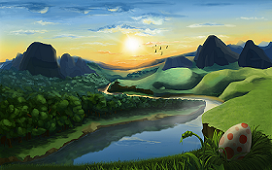
\includegraphics[width=0.7\textwidth]{imgs/sam.png}
	\caption{典型存储器层次结构中的级别,图中上部为服务器计算机中的层次结构,下部为 PMD(个人移动
            设备)中的层次结构。存储器级别离处理器越远,速度越慢、容量越大。注意,时间单位改变了
            10°倍(从皮秒变为毫秒),容量单位改变了102倍(从字节到百万兆字节)。PMD的时钟频率较
            低,缓存和主存储器较小。服务器与桌面计算机的主要区别是以磁盘存储作为层次结构中的最低
            层级,而 PMD 则采用以 EEPROM 技术制造的 Flash 作为最低层级}
\end{figure}

由于快速存储器非常昂贵,所以将存储器层次结构分为几个级别—越接近处理器,容量
越小、速度越快、每字节的成本也越高。其目标是提供一种存储器系统,每字节的成本几乎与
最便宜的存储器级别相同,速度几乎与最快速的级别相同。在大多数(但并非全部)情况下,
低层级存储器中的数据是其上一级存储器中数据的超集。这一性质称为包含性质,层次结构的
最低级别必须具备这一性质,如果这一最低级别是缓存,则由主存储器组成,如果是虚拟存储
器,则由磁盘存储器组成。

随着处理器性能的提高,存储器层次结构的重要性也在不断增加。图 2-2 是单处理器性能
和主存储器访问次数的历史发展过程。处理器曲线显示了平均每秒发出存储器请求数的增加(即
两次存储器引用之间延迟值的倒数),而存储器曲线显示每秒 \verb|DRAM| 访问数的增加(即 \verb|DRAM|
访问延迟的倒数)。在单处理器中,由于峰值存储器访问速度要快于平均速度(也就是图中绘制
的速度),所以其实际情况要稍差一些。

\begin{figure}[!htb]
    \centering
	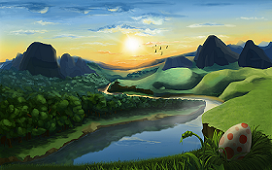
\includegraphics[width=0.7\textwidth]{imgs/sam.png}
	\caption{以 1980年的性能为基准,处理器的存储器请求(对于单处理器或单核心)与 DRAM访问延迟之
            间性能差距的时间变化曲线,该差距是通过测量存储请求数和 DRAM访问数目得出的。注意,
            为了记录处理器与 DRAM性能差距的大小,纵轴必须采用对数刻度。存储器基准为1980年的64
            KB DRAM,延迟性能每年改进1.07(见表2-2)。处理器曲线假定1986年之前每年改进1.25,2000
            年之前每年改进1.52,2000~2005年每年改进1.20,2005~2010年处理器性能没有变化,见第1
            章的图 1-1}
\end{figure}

近来,高端处理器已经转向多核,与单核相比,进一步提高了带宽需求。事实上,总峰值
带宽基本上随核心个数的增大而增大。现代高端处理器(比如 \verb|Intel Core i7|)每个时钟周期可以
由每个核心生成两次数据存储器引用,i7有4个核心,时钟频率为\verb|3.2GHz|,除了大约128亿次
128 位指令引用的峰值措令要求之外,每秒最多还可生成256亿次64位数据存储器引用;总峰
值带宽为\verb|409.6 GB/s|!这一难以置信的高带宽是通过以下方法实现的:实现缓存的多端口和流
水线;利用多级缓存,为每个核心使用独立的第一级缓存,有时也使用独立的第二级缓存;在
第一级使用独立的指令与数据缓存。与其形成鲜明对比的是,DRAM主存储器的峰值带宽只有
它的 \verb|6%|(\verb|25 GB/s|)。

传统上,存储器层次结构的设计人员把重点放在优化存储器平均访问时间上,这一时间是由
缓存访问时间、缺失率和敏失代价决定的。但最近,功率已经成为设计人员的主要考虑事项。在
高端微处理器中,可能有\verb|10MB|或更多的片上缓存,大容量的第二或第三级缓存会消耗大量功率,
既可能是在没有操作时作为泄露功率(称为静态功率),也可能是在执行读取或写人时的活动功
率(称为动态功率),如2.3节所示。这一问题在 PMD的处理器中甚至更为突出,它的CPU的主
动性较低,功率预算可能降至\verb|1/20~1/50|。在此类情况下,缓存消耗的功率可能占总功耗的\verb|25%~50%|。
因此,需要更多地考虑性能与功率之间的权衡,在本章将对这两个因素进行研究。

\subsubsection{存储器层次结构基础:快速回顾}

前面曾经提到,存储器性能和处理器性能之间的差距越来越大,这一点越来越重要,所以
存储器层次结构的基础知识已经出现在计算机体系结构本科课程中,甚至还出现在操作系统和
编译器的相关课程中。因此,我们将首先快速回顾一下缓存及其操作。不过,本章的主要内容
是介绍一些用来应对处理器-存储器性能差距的更高级创新技术。

如果在缓存中找不到某一个字,就必须从层次结构的一个较低层级(可能是另一个缓存,
也可能是主存储器)中去提取这个字,并把它放在缓存中,然后才能继续。出于效率原因,会
一次移动多个字,称为块(或行),这样做还有另外一个原因:由于空间局域性原理,很可能马
上就会用到这些学。每个缓存块都包括一个标记,指明它与哪个存储器地址相对应。

在设计时需要作出一个非常重要的决策:哪些块(或行)可以放在缓存中。最常见的方案
是\verb|组相联|,其中组是指缓存中的一组块。一个块首先被映射到一个组上,然后可以将这个块放
到这个组中的任意位置。要查找一个块,首先将这个块的地址映射到这个组,然后再搜索这个
组(通常为并行搜索),以找到这个块。这个组是根据数据地址选择的:

\begin{equation}
    (Block address) MOD (Number of sets in cache)
\end{equation}

如果组中有n个块,则缓存的布局被称为\verb|n路组相联|。组相联的端点有其自己的名字。\verb|直接映射缓存|
每组中只有一个块(所以块总是放在同一个位置),全相联缓存只有一个组(所以块可以
放在任何地方)。

要缓存只读数据是一件很容易的事情,这是因为缓存和存储器中的副本是相同的。缓存写
入难一些;比如,缓存和存储器中的副本怎样才能保持一致呢?共有两种主要策略。一种是直
写(write-through)缓存,它会更新缓存中的项目,并直接写入主存储器,对其进行更新。另一
种是回写(write-back)缓存,仅更新缓存中的副本。在马上要替换这个块时,再将它复制回存
储器。这两种写入策略都使用了一种写缓冲区,将数据放入这个缓冲区之后,马上就可以进行
缓存操作,不需要等待将数据写入存储器的全部延迟时间。

为了衡量不同缓存组织方式的优劣,可以采用一个名为\verb|缺失率|的指标。\verb|缺失率|是指那些未
能找到预期目标的缓存访问所占的比例,即未找到目标的访问数目除以总访问数目。

为了深刻理解高缺失率的原因,从而更好地设计缓存,一种“3C”模式将所有这些缺失情
景分为以下三个简单的类别。

\begin{itemize}
    \item 强制(Compulsory):对一个数据块的第一次访问,这个块不可能在缓存中,所以必须将
    这个块调人缓存中。即使拥有无限大的缓存,也会发生强制缺失。
    \item 容量(Capacity):如果缓存不能包含程序运行期间所需要的全部块,就会因为有些块被
    放弃,之后再被调入,从而导致容量缺失(还有强制缺失)。
    \item 冲突(Contlict):如果块放置策略不是全相联的,如果多个块映射到一个块的组中,对
    不同块的访问混杂在一起,一个块可能会被放弃,之后再被调人,从而发生冲突缺失(还
    有强制缺失和容量缺失)。
\end{itemize}

表B-4和图B-5是根据3C模型对缓存缺失进行分解后,各种缓存觖失的相对频率。在第3
章和第5章将会看到,多线程和多核都增加了缓存的复杂性,都加大了出现容量缺失的可能性,
而且还因为缓存刷新增加了第4个C\dash 一致性(Coherency)缺失,之所以进行缓存刷新是内
了保持多处理器中多个缓存的一致性;我们将在第5章考虑这些问题。

要小心,缺失率可能会因为多个原因而产生误导。因此,一些设计人员喜欢测量每条指令
的缺失次数,而不是每次存储器引用的缺失次数(缺失率)。这两者之间的关系如下:
\begin{equation}
    \frac{Misses}{Instruction} = \frac{Miss rate \times Memory accesses}{Instruction count} = Miss rate \times \frac{Memory accesses}{Instruction}
\end{equation}

(为了避免出现小数,通常用每1000条指令的缺失次数来表示这一指标,使其变为整数形式。)
这两种度量指标的问题在于它们都没有考虑缺失成本的因素。一种更好的度量指标是存储
器平均访问时间:
\begin{equation}    
    Average memory access time = Hit time + Miss rate \times Miss penalty
\end{equation}

其中,\emph{命中时间}是指在缓存中命中目标花费的时间,\emph{缺失代价}是从内存中替代块的时间(即缺
失成本)。存储器平均访问时间仍然是一个间接性能测量指标,尽管它比缺失率好一些,但不能
代替执行时间。在第3章,我们将会看到推理处理器可以在缺失期间执行其他指令,从而降低
实际缺失代价。多线程的使用(将在第3章介绍)也允许一个处理器容忍一些缺失,而不会被
强制转入空闲状态。我们稍后将会研究,为了利用这些容忍延迟的技术,就需要一些缓存,以
便在处理一次未完成缺失时为请求提供服务。

如果读者是新接触这一资料,或者说这一快速回顾浏览过快,可以参阅附录B。它更深
入地涵盖了同一介绍性内容,并包括一些真实计算机的缓存示例,还对其有效性进行了量化
评估。

\begin{figure}[!htb]
    \centering
	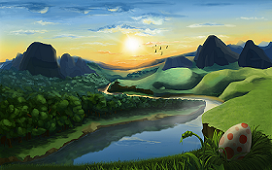
\includegraphics[width=0.7\textwidth]{imgs/sam.png}
	\caption{图2-3 访问时间通常会随着缓存大小和相联程度的增大而增加。这些数据来自 Tarjan、Thoziyoor 和
            Jouppi[2005]提出的CACTI模型6.5。这些数据假定采用40 nm 制程(介于Intel 最快速i7和第二
            快速 i7所用技术之间,与最快速的 ARM 嵌人处理器所用技术相同)、单一存储器组、块大小为
            64字节。由于对缓存布局所做的假定,以及在互连延迟(通常取决于正在访问的缓存块的大小)
            和标记检查与多工之间的复杂权衡,会得到一些有时看起来令人惊奇的结果,比如对于两路组相
            联的64KB缓存,其访问时间会低于直接映射。与此类似,当缓存大小增大时,八蹄组相联产生
            的结果也会导致一些不同寻常的行为。由于这些观察结构都严重依赖于技术和具体设计假定,所
            以诸如 CACTI之类的工具用于缩小权衡过程的搜索空间,而不是对权衡结果进行准确分析}
\end{figure}

附录B的B.3节给出了6种基本的缓存优化方法,我们在此概括性地看一下。这个附录给
出了这些优化方法收益的量化示例。我们还将对这些折中的功率因素进行简要评述。

\begin{enumerate}
    \item \textbf{增大块以降低缺失率}。这是降低缺失率的最简单方法,它利用了空间局域性,并增大了
    块的大小。使用较大的块可以减少强制缺失,但也增加了缺失代价。因为较大块减少了标记数
    目,所以它们可以略微降低静态功率。较大块还可能增大容量缺失或冲突缺失,特别是当缓存
    较小时尤为如此。选择合适的块大小是一项很复杂的权衡过程,具体取决于缓存的大小和缺失
    代价。
    \item \textbf{增大缓存以降低缺失率}。要减少容量缺失,一个显而易见的方法就是增大缓存容量。其
    缺点包括可能会延长较大缓存存储器的命中时间,增加成本和功率。较大的缓存会同时增大静
    态功率和动态功率。
    \item \textbf{提高相联程度以降低缺失率}。显然,提高相联程度可以减少冲突缺失。较大的相联程度
    是以延长命中时间为代价的。稍后将会看到,相联程度也会增大功耗。
    \item \textbf{采用多级缓存以降低缺失代价}。是加快缓存命中速度,以跟上处理器的高速时钟频率,
    还是加大缓存,以缩小处理器访问和主存储器访问之间的差距,这是一个艰难的决策。在原缓
    存和存储器之间加人另一级缓存可以降低这一决策的难度(见图2-3)。第一级缓存可以非常小,
    足以跟上快速时钟频率,而第二级(或第三级)缓存可以非常大,足以收集容纳许多本来要对
    主存储器进行的访问。为了减少第二级缓存中的缺失,需要采用更大的块、更大的容量和更高
    的相联程度。与一级总缓存相比,多级缓存的功率效率更高。如果用L1 和L.2分别指代第一级
    和第二级缓存,可以将平均存储器访问时间重新定义为:
    \begin{equation}
        {Hit time}_{L1} + {Miss rate}_{L1} \times ({Hit time}_{L2} + {Miss rate}_{L2} \times {Miss penalty}_{L2})
    \end{equation}
    \item \textbf{为读取缺失指定高于写入操作的优先级,以降低缺失率}。写缓冲区是实现这一优化的好
    地方。因为写缓冲区拥有在读取缺失时所需位置的更新值,所以写缓冲区存在隐患,即通过存
    储器进行先写后读的隐患。一种解决方案就是在读取缺失时检查写缓冲区的内容。如果没有冲
    突,如果存储器系统可用,则在写入操作之前发送读取请求会降低缺失代价。大多数处理器为
    读取指定的优先级要高于写入操作。这种选择对功耗几乎平没有什么影响。
    \item \textbf{在缓存索引期间避免地址转换,以缩短命中时间}。缓存必须妥善应对从处理器虚拟地址
    到访问存储器的物理地址之间的转换。(虚拟存储器在2.4节和B.4节介绍。)一种常见的优化方
    法是使用页偏移地址(虚拟地址和物理地址中的相同部分)来索引缓存,如附录B所述。这种
    虚拟素引/物理标记方法增加了某些系统复杂度以及(或者)对\verb|L1|缓存大小与结构的限制,但
    从关键路径消除转换旁视缓冲区(\verb|TLB|)访问这一优点抵得过这些敏点。
\end{enumerate}

注意,上述6种优化方法中,每一种都有自己潜在的弱点,可能会导致存储器平均访问时
间的延长,而不是缩短。

本章后续部分假定读者熟悉上述材料及附录B 中的详细内容。在“融会贯通”一节中,我
们将研究 \verb|Intel Core i7| 的存储器层次结构,\verb|Intel Core i7|是一种为高端服务器设计的微处理器,
还将研究 \verb|Arm Cortex-A8| 的存储器层次结构,\verb|Arm Cortex-A8|是一种 PMD设计的处理器,它
是 \verb|Apple iPad|和几种高端智能手机所用处理器的基础。由于这些处理器是为不同计算机应用而
设计的,所以每一类采用的方法都有明显的不同。与桌面计算机中使用的 Intel处理器相比,服
务器中使用的高端处理器拥有更多的核心和更大的缓存,但这些处理器的体系结构是类似的。
差异性主要体现在性能和工作负载的性质上,桌面计算机在某一时刻只有一位用户,主要在操
作系统的顶层运行一个程序,而服务器计算机可能会同时拥有数百位运行几十个应用程序的用
户。由于这些工作负载的差异性,桌面计算机通常更多地考虑存储器层次结构带来的平均延迟,
而服务器计算机还要考虑存储器带宽。即使同为桌面计算机,也是品种繁多,既有低端的上网
本(其处理器有所缩减,类似于高端 PMD中使用的处理器),也有高端桌面计算机,其处理器
包括多个核心,组成方式与低端服务器类似。

与之相对,PMID不但只为一位用户提供服务,而且其操作系统通常要更小一些,通常很少
采用多任务工作方式(同时运行几个应用程序),应用程序也要更简单一些。另外,PMD通常
采用闪存而不是磁盘,大多要同时考虑性能和能耗,能耗决定着电池寿命。

\section{缓存性能的10种高级优化方法}
上面的存储器平均访问时间公式提供了三种缓存优化度量:命中时间、缺失率和缺失代价。
根据最近的发展趋势,我们向这个列表中添加了缓存带宽和功耗两个度量。根据这些度量,可
以将我们研究的10种高级缓存优化方法分为以下5类。

\begin{enumerate}
    \item \textbf{缩短命中时间}。小而简单的第一级缓存和路预测。这两种技术通常还都能降低功耗。
    \item \textbf{增加缓存带宽}。流水化缓存、多组缓存和无阻塞缓存。这些技术对功耗具有不确定影响。
    \item \textbf{降低缺失代价}。关键字优化,合并写缓冲区。这两种优化方法对功率的影响很小。
    \item \textbf{降低缺失率}。编译器优化。显然,缩短编译时间肯定可以降低功耗。
    \item \textbf{通过并行降低缺失代价或缺失率}。硬件预取和编译器预取。这些优化方法通常会增加功
    耗,主要是因为提前取出了未用到的数据。
\end{enumerate}

一般来说,在采用这些技术方法时,硬件复杂度会增加。另外,这些优化技术中有几种需
要采用高级编译器技术。后面将在表2-1中总结这10种技术的实现复杂度和性能优势。对其中
比较简单的优化方法仅作简单介绍,而对其他技术将给出更多描述。

\subsection{第一种优化:小而简单的第一级缓存,用以缩短命中时间、降低功率}
提高时钟频率和降低功率的双重压力都推动了对第一级缓存大小的限制。与此类似,使用
较低级别的相联度,也可以缩短命中时间、降低功率,不过这种权衡要比限制大小涉及的权衡
更复杂一些。

缓存命中过程中的关键计时路径由3个步骤组成:使用地址中的索引确定标记存储器的地
址,将读取的标签值与地址进行比较。接下来,如果缓存为组相联缓存,则设置多路转换器以
选择正确的数据项。直接映射的缓存可以将标记核对与数据传输重叠起来,有效缩短命中时间。
此外,在采用低相联度时,由于减少了必须访问的缓存行,所以通常还可以降低功率。

尽管在各代新型微处理器中,片上缓存的总数已经大幅增加,但由于大容量L1缓存带来的
时钟频率影响,所以L1缓存大小最近的涨幅很小,甚至根本没有增长。选择相联度时的另一个
考虑因素是消除地址别名的可能性;我们稍后对此进行讨论。

使用 \verb|CAD| 工具,可以在制造芯片之前判断各项选择对命中时间和功耗的影响。\verb|CACTI| 程
序可以在 \verb|CMOS| 微处理器上估算各种缓存结构的访问时间和能耗,它的详细程度在 \verb|CAD| 工具
中排在前十名之内。对于一个给定的最小工艺尺寸,\verb|CACTI| 估算在不同缓存大小、相联度、读/
写端口数目和更复杂参数条件下的缓存命中时间。根据缓存大小的不同,对于模型建议的这些
参数,直接映射的命中时间略快于两路组相联,两路组相联四路的 1.2倍,四路组相联是八
路的1.4倍。当然,这些估计值受技术及缓存大小的影响。

\begin{exercise}
    利用图2-3和附录B中表B-4中的数据,判断32KB四路组相联L1缓存的存储器
    访问时间是否快于32 KB两路组相联L1缓存器。假定L.2 的缺失代价是快速L1
    缓存访问时间的15倍。忽略超出L.2 之外的缺失。哪种缓存的存储器平均缓存时
    间较短?
\end{exercise}

\begin{solution}
    设两路组相联缓存的访问时间为1。则,对于两种缓存:

    存储器平均访问时间需哪二命中时间+觖失率 ×缺失代价
    =1+0.038×15=1.57

    对于四路缓存,访问速度是它的1.4倍。缺失代价占用的时间为 15/1.4=10.1。为简
    单起见,设其为10:

    存储器平均访问时间四命中时间邮路×1.4+缺失率 ×缺失代价
    =1.4+0.037×10-=1.77

    显然,采用较高的相联度看起来是一种糟糕的权衡选择;不过,由于现代处理器
    中的缓存访问通常都实现了流水化,所以很难评估对时钟周期时间的确实影响。
\end{solution}

如图2-4所示,在选择缓存大小和相联度时,能耗也是一个考虑因素。在\verb|128KB|或\verb|256 KB|
缓存中,当从直接映射变到两路组相联时,高相联度的能量消耗从大于2变到可以忽略。

\begin{figure}[!htb]
    \centering
	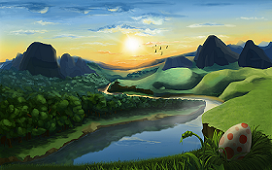
\includegraphics[width=0.7\textwidth]{imgs/sam.png}
	\caption{每次读取操作的能耗随缓存大小、相联度的增加而增加。和图2-3一样,使用CACTI对相同技术
            参数进行建模。八路组相联缓存的代价之所以很高,是因为并行读取8个标签及相应数据的成本
            造成的}
\end{figure}

在最近的设计中,有三种其他因素导致了在第一级缓存中使用较高的相联度。第一,许多
处理器在访问缓存时至少需要两个时钟周期,因此命中时间较长可能不会产生太过严重的影响。
第二,将 TLB排除在关键路径之外(TLB带来的延迟可能要大于高相联度导致的延迟),几乎
所有L1缓存都应当是变址寻址的。这就将缓存的大小限制为页大小与相联度的乘积,这是因为
只有页内的位才能用于变址。在完成地址转换之前对缓存进行变址的问题还有其他一些解决方
案,但提高相联度是最具吸引力的一种,它还有其他一些好处。第三,在引入多线程之后(参
见第3章),冲突缺失会增加,从而使提高相联度更具吸引力。

\subsection{第二种优化:采用路预测以缩短命中时间}

这是另外一种可以减少冲突缺失,同时又能保持直接映射缓存命中速度的方法。在路预测
技术中,缓存中另外保存了一些位,用于预测下一次缓存访问组中的路或块。这种预测意味着
尽早设定多工选择器,以选择所需要的块,在与缓存数据读取并行的时钟周期内,只执行一次
标签比较。如果缺失,则会在下一个时钟周期中查看其他块,以找出匹配项。

在一个缓存的每个块中都添加块预测位。根据这些位选定要在下一次缓存访问中优先尝试
哪些块。如果预测正确,则缓存访问延迟就等于这一快速命中时间。如果预测错误,则尝试其
他块,改变路预测器,延迟会增加一个时钟周期。模拟表明,对于一个两路组相联缓存,组预
测准确度超过90\%;对于四路组相联缓存,超过80\%,对I-缓存的准确度优于对D-缓存的准确
度。如果路预测能够至少快10\%(这是非常可能的),路预测方法可以缩短两路组相联缓存的存
储器平均访问时间。路预测最早于20世纪90年代中期应用在 \verb|MIPS R10000| 中。这在使用两路
组相联缓存的处理器中很常见,在使用四路组相联缓存的ARM \verb|Cortex-A8| 中也采用了这一技术。
对于非常快速的处理器,要实现一个周期的时延是非常具有挑战性的,而这对于降低路预测代
价非常关键。

还有一种扩展形式的路预测,它使用路预测位来判断实际访问的缓存块,可以用来降低功
耗(路预测位基本上就是附加地址位);这种方法也可称为路选择,当路预测正确时,它可以节
省功率,但在路预测错误时则会显著增加时间,这是因为需要重复进行访问,而不仅是重复标
记匹配与选择过程。这种优化方法只有在低功率处理器中才可能有意义。Inoue、Ishihara 和
Murakasi [1999]根据 SPEC95基准测试进行估算,对于四路组相联缓存使用路选择方法,可以
使1-缓存的平均访问速度提高1.04倍,D-缓存提高1.13倍,与正常的四路组相联缓存相比,
I-缓存的平均缓存功耗降为原来的 0.28,D-缓存降为0.35。路选择方法的一个重要缺点就是它
增大了实现缓存访问流水化的难度。

\begin{exercise}
    假定在一个普通四路组相联实现中,D-缓存访问次数是1-缓存访问次数的一半,
    1-缓存和 D-缓存分别占该处理器功耗的25\%~15\%。根据上述研究的估计值,判
    断路选择方法是否提高了每瓦功耗的性能。
\end{exercise}

\begin{solution}
    对于1-缓存,节省的功率为总功率的25×0.28-0.07,对于D-缓存,为1S ×0.35=0.05,
    共节省0.12。路预测版本需要的功率为标准四路缓存的0.88。缓存访问时间的增加
    等于1-缓存平均访问时间的增加量加上D-缓存访问时间增加量的一半,即1.04+0.5
    x0.13=1.11倍。这一结果意味着路选择的性能是标准四路缓存的0.90。因此,路
    选择方法略微提高了每焦功耗的性能,比值为 0.90/0.88=1.02。这一优化方法最适
    合用在看重功率胜于看重性能的情景。
\end{solution}

\subsection{第三种优化:实现缓存访问的流水化,以提高缓存带宽}

这种优化方法就是实现缓存访问的流水化,使第一级缓存命中的实际延迟可以分散到多个
时钟周期,从而缩短时钟周期时间、提高带宽,但会减缓命中速度。例如,对于20世纪90年
代中期的 Intel Pentium处理器,指令缓存访问的流水线需要1个时钟周期,对于从 20世纪90
年代中期到2000年的 Pentium Pro 到 Pentium II,需要2个时钟周期,对于2000年出现的 Pentium4
和现在的 Intel Core 17,需要4个时钟周期。这一变化增加了流水线的段数,增加了预测错误分
支的代价,延长了从发出载入指令到使用数据之间的时钟周期数(参见第3章),但的确更便于
采用高相联度的缓存。

\subsection{第四种优化:采用无阻塞缓存,以提高缓存带宽}

对于允许乱序执行(在第3章讨论)的流水化计算机,其处理器不必因为一次数据缓存觖失
而停顿。例如,在等待数据缓存返回缺失数据时,处理器可以继续从指令缓存中提取指令。无阻
塞缓存(或称为自由查询缓存)允许数据缓存在一次缺失期间继续提供缓存命中,进一步加强
了这种方案的潜在优势。这种“缺失时仍然命中”优化方法在缺失期间非常有用,它不会在此期
间忽略处理器的请求,从而降低了实际缺失代价。还有一种精巧而复杂的选项:如果能够重叠多
个缺失,那缓存就能进一步降低实际缺失代价,这种选项被称为“多次缺失时仍然命中"(hit under
multiple miss) 或者“缺失时缺失”(miss under miss)优化方法。只有当存储器系统可以为多次
缺失提供服务时,第二种选项才有好处,大多数高性能处理器(比如 Intel Core i7)通常都支持
这两种优化方法,而低端处理器,比如 ARMA8,仅在L.2提供了有限的无阻塞支持。

为了研究无阻塞缓存在降低缓存缺失代价方面的有效性,Farkas 和Jouppi [1994]做了一项
研究:假定8KB缓存的缺失代价为14个周期;在缺失情况下允许一次命中时,他们都观测到
实际缺失代价的降低,对于 SPECINT92 基准测试降低20%,对于 SPECFP92 基准测试降低30%。
Li、Chen、Brockman 和 Jouppi2011]最近对这一研究内容进行了更新,他们采用多级缓存,
根据最近的技术情况对缺失代价作出了假设,并采用了规模更大、要求更严格的 SPEC2006 基准
测试。这项研究采用一种基于 Intel i7单核心的模型(见2.6节)运行 SPEC2006基准测试。图2-5
显示了一次缺失时允许1、2、64次命中时,数据缓存访问延迟的降低情况。自从研究早期就采用
了大缓存容量、增加了L.3缓存,所以采用“缺失时命中”的好处显得不够明显,SPECINT2006
基准测试显示缓存延迟平均降低大约9%,而采用 SPECFP2006 基准测试结果大约为12.5%。

例题
解答
对于浮点程序来说,主数据缓存的两路组相联和一次缺失时仍然命中,哪个更重
要一些?对整数程序来说呢?假定32KB数据缓存的平均缺失率如下:对于采用
直接映射缓存的浮点程序为5.2%,对于采用两路组相联缓存的浮点程序为4.9%,
采用直接映射缓存的整数程序为 3.5%,对于采用两路组相联缓存的整数程序为
3.2%。假定1.2的缺失代价为10个周期,L2的缺失率和缺失代价相同。

对于浮点程序,存储器平均停顿时间为
缺失率 D ×缺失代价=5.2% × 10=0.52
缺失率两略 ×缺失代价=4.9%×10=0.49
两路相联缓存的访问延迟(包括停顿)为0.49/0.52,或者为直接映射缓存的94%。
图2-5的标题表明允许一次缺失时仍然命中,可以将浮点程序的平均数据缓存访问
延迟缩短为一次阻塞缓存的87.5%。因此,对于浮点程序而言,支持一次缺失时仍
然命中一次的直接映射数据缓存,在性能上要优于在缺失时阻塞的两路相联缓存。

对于整数程序,计算如下:
缺失率 DM ×缺失代价=3.5% ×10=0.35
缺失率两路× 缺失代价=3.2%×10=0.32
两种组相联缓存的数据缓存访问延迟为 0.32/0.35,或直接映射缓存的91%,
而在一次缺失时允许一次命中可以将访问延迟降低9%,使两种选择的性能大
体相当。

\begin{figure}[!htb]
    \centering
	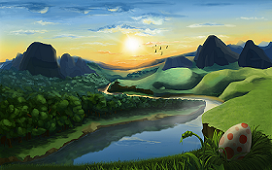
\includegraphics[width=0.7\textwidth]{imgs/sam.png}
	\caption{用9个 SPECINT(左)和9个 SPECFP(右)基准测试评估在1、2或64次缓存缺
            失时仍然允许命中情况下非阻塞缓存的效果。这个数据存储器系统以 Intel i7建模,它
            包括32KBL.1缓存,访问延迟为4个周期。I.2缓存(与指令共享)为256KB,访问
            延迟为10个时钟周期。L3为2MB,访问延迟为35个周期。所有访问都是八路组相
            联,大小为64字节块大小。在缺失时允许一次命中可以使整数基准测试的缺失代价
            降低9\%,浮点基准测试降低12.5\%。允许第二次命中会将这些结果提高 10\%~16\%,
            得到64个没有多少额外改进的结果}
\end{figure}

对非阻塞缓存进行性能评估时,真正的难度在于一次缓存缺失不一定会使处理器停顿。在
这种情况下,很难判断一次缺失造成的影响,因此也就难以计算存储器平均访问时间。实际缺
失代价并不等于这些缺失时间之和,而是处理器的非重叠停顿时间。非阻塞缓存的优势评估非
常复杂,因为它取决于存在多次缺失时的缺失代价、存储器引用模式以及处理器在有未处理缺
失时能够执行多少条指令。

通常,对于一个能够在L.2缓存中命中的L.1 数据缓存缺失,乱序处理器能够隐藏其大部分
缺失代价,但不能隐藏更低层次缓存敏失的大部分代价。而在决定支持多少个未处理缺失时,
需要考虑多种因素,如下所述。

\begin{itemize}
    \item 缺失流中的时间与空间局域性,它决定了一次缺失是否会触发对低级缓存或对存储器的
    新访问操作。
    \item 对访问请求作出回应的存储器或缓存的带宽。
    \item 为了允许在最低级别的缓存中出现更多的未处理缺失(在这一级别的缺失时间是最长
    的),需要在较高级别上支持至少数目相等的缺失,这是因为这些失必须在最高级别缓
    存上启动。
    \item 存储器系统的延迟。
\end{itemize}

下面这个简化示例表明了这一关键思想。
例题
假定主存储器的访问时间为36ns,存储器系统的持续传输速率为16GB/s。设块大
小为64字节,如果在给定请求流的情况下能够保持峰值带宽,而且访问永远不会
冲突,则需要支持的最大未完成缺失数目为多少?如果一次引用与前4次引用发
生冲突的概率为 50%,估计最大未完成引用数目。为简单起见,忽略缺失之间的
时间。

解答
在第一种情况下,假定我们可以保持峰值带宽,存储器系统可以支持每秒(16x
10)%64-250百万次引用。由于每次引用耗时36ns,因此可以支持250 ×10°×36x
10--9次引用。如果发生冲突的概率大于0,由于我们不能在这些引用时开始工
作,所以需要更多的未完成引用;存储器系统需要的独立引用数应当更多而不是
更少!为了估计这一数目,可以假定有一半存储器引用不需要发送到存储器。这
就意味着必须能够支持两倍数量的未完成引用,即18次。

Li、Chen、Brockman 和 Jouppi在研究中发现:对于在缺失时允许1次命中的情况,整数程
序的CPI 减少大约7%,而在允许64 次命中时,减少大约12.7%。对于浮点程序,允许1次命
中时减少12.7%,64 次时减少17.8%。这些减少数值与图2-5中所示数据缓存访问延迟的减少
值非常接近。

\subsection{第五种优化:采用多种缓存以提高缓存带宽}
我们可以将缓存划分为几个相互独立、支持同时访问的缓存组,而不是将它们看作一个整
体。分组方式最初用于提高主存储器的性能,现在也用于 DRAM 芯片和缓存中。Arm Cortex-A8
在其L2缓存中支持1至4个缓存组;Intel Core i7 的L1 中有4个组(每个时钟周期内可以支持
2次存储器访问),L2有8个组。

显然,当访问请求很自然地分布在缓存组之间时,分组方式的效果最佳,所以将地址映射
到缓存组的方式影响着存储器系统的行为。一种简单有效的映射方式是将缓存块地址按顺序分
散在这些缓存组中,这种方式称为顺序交错。例如,如果有4个缓存组,0号缓存组中的所有
缓存块地址对4求模后余0,1号缓存组中的所有缓存块地址对4求模后余1,以此类推。图2-6
显示了这种交错方式。采用分组方式还可以降低缓存和 DRAM 中的功耗。


图2-6 使用块寻址的四路交错缓存组。假定每个块64个字节,这些地址需要分别
乘以64 才能实现字节寻址

\subsection{第六种优化:关键字优先和提前重启动以降低缺失代价}
这一技术的事实基础是人们观测到处理器在某一时刻通常仅需要缓存块的一个字。这一策
略显得“不够耐心”:无须等待完成整个块的载入过程,一旦载人被请求字之后,立即将其发出,
然后就重启处理器。下面是两个特定策略。

\begin{itemize}
    \item 关键字优先:首先从存储器中请求缺失的字,在其到达缓存之后立即发给处理器;使处
    理器能够在载入块中其他字时继续执行。
    \item 提前重启动:以正常顺序提取字,但只要块中的被请求字到达缓存,就立即将其发送给
    处理器,让处理器继续执行。
\end{itemize}

通常,只有在采用大型缓存块的设计中,这些技术才有用武之地,如果缓存块很小,它们
带来的好处是很低的。注意,在载人某个块中的其余内容时,缓存通常可以继续满足对其他块
的访问请求。

不过,根据空间局域性原理,下一次引用很可能就会指向这个块的其余内容。和非阻塞
缓存一样,其缺失代价的计算也不是非常容易。在采用关键字优先策略时,如果存在第二次
请求,实际缺失代价等于从本次引用开始到第二部分内容到达之前的非重叠时间。关键字优
先策略和提前重启动策略的好处取决于块的大小以及在尚未获取某部分内容时又出现另一次
访问的机率。

\subsection{第七种优化:合并写缓冲区以降低缺失代价}

因为所有存储内容都必须发送到层次结构的下一层级,所以直写缓存依赖于写缓冲区。
即使是写回缓存,在替代一一个块时也会使用一个简单的缓冲区。如果写缓冲区为空,则数据
和整个地址被写到缓冲区中,从处理器的角度来看,写人操作已经完成;在写缓冲区准备将
字写到存储器时,处理器继续自己的工作。如果缓冲区中包含其他经过修改的块,则检查它
们的地址,看看新数据的地址是否与写缓冲区中有效项目的地址匹配。如果匹配,则将新数
据与这个项目合并在一起。这种优化方法称为写合并。Intel Core i7 和其他许多处理器都采用
了写合并方法。

如果缓冲区已满,而且没有匹配地址,则缓存(和处理器)必须等待,直到缓冲区中拥有
空白项目为止。由于多字写人的速度通常快于每次只写人一个字的写人操作,所以这种优化方
法可以更高效地使用存储器。Skadron 和Clark[1997]发现:即使在一个合并四项的写缓冲区中,
所生成的停顿也会导致5%~10%的性能损失。

这种优化方式还会减少因为写缓冲区已满而导致的停顿。图2-7显示了一个写缓冲区在采
用和不采用写合并时的情况。假定这个写缓冲区中有四项,每一项有4个 64位的字。在来用
这一优化方法时,图中的4个字可以完全合并,放在写缓冲区的一个项目中,而在不采用这一
优化方法时,对写缓冲区的连续地址执行4次存储操作,将整个缓冲区填满,每个项目中保存
一个字。

注意,输人/输出设备寄存器经常被映射到物理地址空间。由于1/O寄存器是分享的,不能
像存储器中的字数组那样操作,所以这些1/O地址不能允许写合并。例如,它们可能要求为每
个 1O 寄存器提供一个地址和一个数据字,而不能只提供一个地址进行多字写人。为了实现这
些副作用,通常由缓存将这些页面进行标记,表明其需要采用非合并直写方式。

图2-7 为了说明写合并过程,上面的写缓冲区未采用该技术,下面的写缓冲区采用了这一技术。在进行
合并时,4次写人内容被合并到一个缓冲区项目中;而未进行合并时,4次写人操作就填满了整个
缓冲区,每个项目的四分之三被浪费。这个缓冲区有四个项目,每一项保存4个64位字。每个项
目的地址位于左侧,有效位(V)指明这个项目的下面8个连续字节是否被占用(未采用写合并
时,图中上半部分右侧的字只会用于同时写多个字的指令。)

\subsection{第八种优化:采用编译器优化以降低缺失率}
前面介绍的技术都需要改变硬件。下面这种技术可以在不做任何硬件改变的情况下降低续
失率。

这种神奇的降低效果来自软件优化—硬件设计人员最喜爱的解决方案!处理器与主存储
器之间的性能差距越拉越大,已经促使编译器编写人员深入研究存储器的层次结构,以了解能
否通过编译时间优化来提高性能。同样,研究内容包括两个方面:指令缺失性能改进和数据缺
失性能改进。下面给出的优化技术在很多现代编译器中均有应用。

1. 循环交换
一些程序中存在嵌套循环,它们会以非连续顺序访问存储器中的数据。只要交换一下这些
循环的嵌套顺序,就可能使程序代码按照数据的存储顺序来访问它们。如果缓存中无法容纳这
些数组,这一技术可以通过提高空间局域性来减少缺失;通过重新排序,可以使缓存块中的数
据在被替换之前,得到最大限度的充分利用。例如,设x是一个大小为[5000,100]的两维数据,
其分配方式使得×[1,J]和x[1,J+2]相邻(由于这个数组是按行进行排列的,所以我们说这种顺
序是以行为主的),以下两段代码说明可以怎样来优化访问过程:

\begin{verbatim}
    /*优化之前*/
    for (j= 0; jc 100;j = j+1)
    for (i= 0; i≤ 5000; i = i+1)
    ×[i1[3]=2*x[E];
    /*优化之后*/
    for (i= 0; i≤ 5000; i = i+1)
    for (j= 0; j< 100; j = j+1)
    x[i[3=2*x[1[3];
\end{verbatim}
原代码以100个字的步幅跳跃式浏览存储器,而修改后的版本在访问了一个缓存块中的所
有字之后才进人下一个块。这一优化方法提高了缓存性能,却没有影响到所执行的指令数目。
2.分块

这一优化方法通过提高时间局域性来减少缺失。这一次还是要处理多个数组,有的数组是
按行来访问的,有的是按列来访问的。由于在每个循环选代中都用到了行与列,所以按行或按
列来存储数组并不能解决问题(按行存储称为行主序,按列存储称为列主序)。这种正交访问方
式意味着在进行循环交换之类的转换操作之后,仍然有很大的改进空间。

分块算法不是对一个数组的整行或整列进行操作,而是对其子矩阵(或称块)进行操作。
其目的是在缓存中载人的数据被替换之前,在最大限度上利用它。下面这段执行矩阵乘法的示
例可以帮助理解这一优化方法的动机:

\begin{verbatim}
    /*优化之前*/
    for (i= 0; i< N;i= i+1)
    for (j= 0; j<N;j= j+1)
    {r= O;
    for (k = O; k< N; k- k+1)
    r= r+ y[i][K]*Z[K[S];
    x[i][j] = r;
    };
\end{verbatim}
两个内层循环读取乙的所有NxN个元素,重复读取y中一行的同一组 N个元素,再写人X
的一行 N个元素。图 2-8是访问这三个数组的一个快照。深色阴影区域表示最近的访问,浅色
阴影区域表示较早的访问,白色表示还没有进行访问。

容量缺失的数目显然取决于N和缓存的大小。如果它能容纳所有这3个N×N矩阵,只要没
有缓存冲突,就一切正常。如果缓存可以容纳一个 NxN矩阵和包含N个元素的一行,则至少y
的第i行和数组可以停留在缓存中。如果缓存的容量更小,那可能对于x和z都会发生觖失。
在最差情况下,进行N次操作可能需要从存储器中读取 2N’+N个字。

图 2-8
三个数组 ×、y和z的快照,其中 N=6,1=1。对数组元素访问的前后时间用阴影表示:白色表
示还没有被访问过,浅色表示较早的访问,深色表示最近的访问。与图2-9相对照,为了计算
x的新元素,会重复读取y和z的元素。在行或列的旁边显示了用于访问这些数组的变量i、了
和k


为了确保正在访问的元素能够放在缓存中,对原代码进行了修改,改为计算一个大小为B
xB的子矩阵。两个内层循环现在以大小为B的步长进行计算,而不是以x和z的完整长度为步
长。B被称为分块因子。(假定x被初始化为0。)
\begin{verbatim}
    /*优化之后*/
    far (jj= 0;j
    《kk = 0;kk <N; kk = kk+B)
    for (i= O; i< N;i- i+l)
    for (j= jj: j < nin(jj+B,N); j = j+1)
    for (k = kk; k ≤ min(kk+B,N); k - k +1)
    r=r+ y[i][k*z[K 3];
    x[i[j] = x[i][j] + r;
    };
\end{verbatim}
图2-9展示了使用分块方法对三个数组的访问。仅观察容量缺失,从存储器中访问的总字
数为2N/B+N。这一总数的改善因素大约为B。由于y获益于空间局域性,2获益于时间局域性,
所以分层方法综合利用了空间局域性和时间局域性。

尽管我们的目标是降低缓存缺失,但分块方法也可用于帮助寄存器分配。通过设定一个
较小的分块大小,使这个块能够保存在寄存器中,可以在最大程度上降低程序中的载入与存
储数量。

在4.8节将会看到,对于以矩阵主要数据结构的程序,要在基于缓存的处理器上获得出色
性能,缓存分块方法是必不可少的。

图 2-9

当B=3时,对数组x、y和z的访问历史。注意,与图2-8相比,访问的元素数目较少

\subsection{第九种优化:对指令和数据进行硬件预取,以降低缺失代价或缺失率}
通过执行过程与存储器访问的重叠,无阻塞缓存有效地降低缺失代价。而另一种方法是在
处理器请求项目之前,预先提取它们。指令和数据都可以预先提取,既可以直接放在缓存中,
也可以放在一个访问速度快于主存储器的外部缓冲区中。

擔令预取经常在缀存外部的硬件中完成。通常,处理器在一次映失时提取两个块:被请求
块和下一个相邻块。被请求块放在它返回时的指令缓存中,预取块被放在指令流缓冲区中。如
果被请求块当前存在于指令流缓冲区中,则原缓存请求被取消,从流缓冲区中读取这个块,并
发出下一条预取请求。

类似方法可应用于数据访问[Jouppi 1990]。Palacharla 和 Kessler [1994]研究了一组科学程序,
并考查了多个可能处理指令或数据的流缓冲区。他们发现,对于一个具有两个64 KB 四路组相
联缓存的处理器(一个用于缓存指令,另一个用于缓存数据),八个流缓冲区可以捕获其所有缺
失的50%~70%。

Intel core i7 支持利用硬件预先提取到L1和L2中,最常见的预取情况是访问下一行。一些
较早的 Intel处理器使用更主动的硬件预取,但会导致某些应用程序的性能降低,一些高级用户
会因此而关闭这一功能。

图2-10显示了在启用硬件预取时,部分SPEC2000 程序的整体性能改进。注意,这一数字
仅包含12个整数程序中的2个,而大多数 SPEC浮点程序则都包含在内。

图 2-10
在 intel Pentium 4上启用硬件预取之后,12个 SPECint2000 基准测试中的2个测试、14个
SPEC p2000 基准测试中的9个测试获得的加速比。图中仅给出从预取中获益最多的程序,对
于图中未给出的15个 SPEC基准测试,预取加速比低于15%[Singhal 2004]
预取操作需要利用未被充分利用的存储器带宽,但如果它干扰了迫切需要的缺失内容,反
而可能会实际降低性能。在编译器的帮助下,可以减少无用预取。当预取操作正常执行时,它
对功率的影响可以怒略。如果未用到预取数据或者替换了有用数据,预取操作会对功率产生非
常负面的影响。

\subsection{第十种优化:用编译器控制预取,以降低缺失代价或缺失率}
作为硬件预取的替代方法,可以在处理器需要某一数据之前,由编泽器插入请求该数据的
预取指令。共有以下两种预取。

\begin{itemize}
    \item 寄存語预取将数据值载入到一个寄存器中。
    \item 缓存预取仅将数据载入到缓存中,而不是寄存器中。
\end{itemize}

这两种预取都可能是故障性的,也都可能是非故障性的;也就是说,其地址可能会导致虚
拟地址错误异常和保护冲突异常,也可能不会导致。利用这一术语,正常的载入指令可能被看
作是“故障性寄存器预取指令”。非故障性预取只是在通常导致异常时转换为空操作,而这正是
我们想要的结果。

最有效的预取对程序来说是“语义透明的”:它不会改变寄存器和存储器的内容,也不会导
致虚拟存储器错误。今天的大多数处理器都提供非故障性缓存预取。本节假定非故障性缓存预
取,也称为非绑定预取。

只有当处理器在预取数据时能够继续工作的情况下,预取才有意义;也就是说,缓存在等
待返回预取数据时不会停顿,而是继续提供指令和数据。可以想到,这些计算机的数据缓存通
常是非阻塞性的。

与硬件控制的预取操作类似,这里的目标也是将执行过程与数据预取过程重叠起来。循环
是重要的预取优化目标,因为它们本身很适于进行预取优化。如果缺失代价很小,编译器只需
要将循环展开一两次,在执行时调度这些预取操作。如果缺失代价很大,它会使用软件流水线
(参见附录H)或者将循环展开多次,以预先提取数据,供后续迭代使用。

不过,发出预取指令会导致指令开销,所以编译器必须非常小心地确保这些开销不会超过
所得到的好处。如果程序能够将注意力放在那些可能导致缓存缺失的引用上,就可以避免不必
要的预取操作,局时明显缩短存储器平均访问时间。

例题
解答
对于以下代码,判断哪些访问可能导致数据缓存缺失。然后,插入预取指令,以减
少缺失。最后,计算所执行的预取指令数目和通过预取避免的缺失数。假设有一个
8KB 直接映射的数据缓存,块大小为16字节,它是一个执行写人分派的写回缓存。
a 和b是双精度浮点数组,所以它们的元素长8个字节。a有3行、100列,b有101
行、3列。另外假定在程序开始时,这些数据没有在缓存中。
\begin{verbatim}
    for (i = 0; 1<3;i= i+1)
    for (j= 0; j< 100; j= j+1)
    a[i[j]- b[jlCo]*b[j+1[0]:
\end{verbatim}
编译器首先判断哪些访问可能导致缓存缺失,否则可能会为那些能够命中的数据发
出预取指令,白白浪费时间。a的元素是以它们在存储器中的存储顺序写人的,所
以a可以受益于空间局域性:j的偶数值会缺失,奇数值会命中。由于a有3行、
100列,所以对它的访问将会导致3×(100/2)=150次缺失。

数组b不会从空间局域性中获益,因为对它的访问不是按照存储顺序执行的。数组
b 可以从时间局域性中获得双重受益:每次对1进行迭代时会访问相同元素,每次
对j进行迭代时使用的b元素值与上一次迭代相同。忽略可能存在的冲突缺失,由
b导致的缺失在1=0时访问bLj+1][0]出现,还有就是在j=0时首次访问b[jE0]出
现。当1=0时,j从0增至99,所以对b的访问将导致100+1=101次缺失。

因此,这次循环将会出现的数据缓存缺失大约包括a的150次和b的101次,也就
是251 次缺失。

为了简化优化过程,我们不用费心为循环中的第一次访问进行预取。这些内容可能
已经放在缓存中了,或者我们需要为a或b的前几个元素承担缺失代价。在到达循
环末尾时,预取操作会尝试提前提取超出a末端之外的内容(a[i][100]

ari][106])和b末端之外的内容(bC101][0]..b[107][0]),我们并不需要费心来禁
用这些预取。如果这是一些故障性预取,那我们也许不能承担如此之大的开销。我
们假定缺失代价非常大,需要至少提前(比如)7次迭代来开始预取。(换句话说,
我们假定在第8次迭代之前进行预取不会得到任何好处。)以下代码中加下划线的
部分,是为了添加预取优化而对前面代码所做的修改。

\begin{verbatim}
    for (j-0: j<100:J=1+1)1
    Prefetch(bli+71O]):
    /* b(J.0) for ! iterations later */
    Prefetch(alO1 li+71)i
    1 a!0.j) fon J iterations_later */
    a01C1-b[j110] *b[j+11[01jl:
    for (i = 1;i≤ 3; i = i+1)
    for (i - o: j < 100: J-j+1){
    Prefetch(aJd] Ti+7]);
    a1.i tor.t/ iterations
    [iJLjl = bljlCoJ * bLj+lJ[oJ;
\end{verbatim}
这一经过修订的代码预取 a[1C7]至 a[1][99]和b[7][0]至 b[100][0],将非预取敏失
的数目减至:
\begin{itemize}
    \item 第一次循环中访问元素 b[0][0],b[1J[0],,b[6][0]时的7次缺失
    \item 第一次循环中访问元素 aC0][0],a[0][1],,a[036]时的4次缺失([7/2])
\end{itemize}
(利用空间局域性将缺失数减少为每16字节缓存块一次缺失)
\begin{itemize}
    \item 第二次循环中访问元素 aC1][0],a[1][1],,a[11[6]的4次缺失([7/2])
    \item 第二次循环中访问元素 a[23[0],a[2][1],,a[2J[6]的4次鍊失([7/2])
\end{itemize}
即总共19次非预取缺失。避免232次缓存毓失的成本是执行了400条预取指令,
这很划算。
例题
计算上面例题中节省的时间。忽略指令缓存缺失,并假定数据缓存中没有冲突缺失
或容量缺失。假定预取过程可以相互重叠,并能与缓存缺失重養。因此可以用最高
存储器带宽传输。下面是忽略缓存缺失的关键循环次数:原循环每次迭代需要7个
时钟周期,第一次预取循环每次迭代需要9个时钟周期,第二次预取循环每次选代
需要8个周期(包含循环外部的开销)。一次缺失需要100个时钟周期。

解答

原来的双层嵌套循环执行3x100-300次。由于该循环每次选代需要7个时钟周期,
所以总共为300 x 7=2100时钟周期再加上缓存缺失。缓存缺失增加 251 × 100-
25 100个时钟周期,总共27 200个时钟周期。第一次预取循环迭代100次,每次迭
代为9个时钟周期,所以总共900个时钟周期再加上缓存缺失。现在加上缓存缺失的
11x 100=1100个时钟周期,总共2000个时钟周期。第二个循环执行2x100-200次,
每次选代为8个时钟周期,所以需要1600个时钟問期,再加上缓存缺失8 × 100=800
个时钟周期。总共2400个时钟周期。由上个例子可以知道,这一代码为了执行这两
个循环,在 2000+2400-4400个时钟周期内执行了400条预取指令。如果我们假定这
些预取操作完全与其他执行过程相重叠,那么这一预取代码要快27200/4400-6.2倍。
尽管数组优化理解起来比较容易,但现代程序更可能使用指针。Luk 和Mowry[1999]已经
证明,基于编译器的预取优化有时也可以扩展到指针。在10个使用递归数据结构的程序中,在
访问一个节点时预取所有指针,可以使半数以上的程序性能提高4%~31%。而另一方面,其他
程序的性能变化不超过原性能的2%。问题症结包括两个方面,一是要预先提取的数据是否已经
存在于缓存中,二是预取数据能否在需要它们时提前到达缓存。

许多处理器支持缓存预取指令,高端处理器(比如 Intel Core i7)还经常在硬件中完成某种
类型的自动预取。

\subsection{缓存优化小结}
用于改进命中时间、带宽、缺失代价及缺失率等性能的技术通常会影响到存储器平均访问
时间公式的其他部分,而且还会影响到存储器层次结构的复杂性。表2-1总结了这些技术,并
估计了它们对复杂性的影响,其中“+”表明该技术会改进该项因素,“\_”表示会损害该项因
素,空白则表示没有影响。一般来说,没有哪种技术能够改进多项因素。

\begin{verbatim}
    表2-1 10种高级缓存优化技术小结,给出了对缓存性能、功耗和复杂度的影响
    技术
    命中
    缺失
    硬件成本/
    时间
    带宽
    缺失率
    功耗
    注
    代价
    复杂度
    小而简单的缓存
    路预测缓存
    流水化缓存访问
    非阻塞缀存
    分组缓存
    释
    很普通、应用广泛
    在Pentium 4中使用
    应用广泛
    应用广泛
    在i7和Cortex-A8的L2中
    使用
    应用广说
    关键字优先和提前
    重启动
    合并写缓冲区
    以编译器技术减少
    缀存缺失
    +
    +
    1
    0
    和直写法一起广泛应用
    软件是一个挑战,但许
    多编译器都能处理常见
    的线性代数计算
    指令与数据的硬件
    预取
    2(指令)
    3(数据)
    大多提供预取指令,现
    代高端处理器还会在硬
    件中实现自动预取
    编译器控制的预取
    需要非阻塞缓存,可能
    存在指令开销,在许多
    CPU中得到应用
\end{verbatim}
*尽管一种技术通常仅能改进一个因素,但如果能够尽早完成,预取可以减少缺失;如果不能尽早完成,則可以減少
敏失代价。“+” 表示该技术会改进该项因素,

“\_”表示会损害该项因素,空白則表示没有影响。复杂度的评估具
有主观性,0表示最容易,了标志着一项挑战。

\section{存储器技术与优化}
…唯一使计算机站稳脚跟的发展成果就是可靠存储器的发明,也就是核心存储器它的
成本在含理范围内,它是可靠的,而且因为它是可靠的,所以能够在适当的时候扩大其容量。[第
209 页]

—Maurice Wilkes
Memoirs ofa Computer Pioneer (1985)

主存储器在层次结构上位于缓存的下一层级。主存储器满足缓存的需求,并充当1/O接口,
既是输人的目的地,又是输出的源头。对主存储器的性能度量同时强调延迟和带宽。传统上,
主存储器延迟(它会影响缓存缺失代价)是缓存的主要考虑因素,而主存储器带宽则是微处理
器和1/O的主要考虑困素。

尽管缓存可以从低延迟存储器中获益,但一般来说,通过新的组织方式来提高存储器带宽
要比降低延迟更容易一些。由于多级缓存日益普及,而且采用较大的分块,使主存储器带宽对
于缓存也非常重要。事实上,缓存设计人员增大块大小就是为了利用更高的存储器带宽。

前面几节描述了可以通过缓存优化来缩小处理器与 DRAM之间的性能差距,但仅仅增大缓
存或增加更多的缓存级别并不能消除这一差距。主存储器也需要进行革新。

在过去,对主存储器的革新就是改变构成主存储器的众多 DRAM 芯片(比如多个存储器组)
的组织方式。在使用存储器组时,通过拓宽存储器或其总线,或者同时加宽两者,可以提供更
大的带宽。但是,具有讽刺意味的是,随着单片存储器芯片容量的增加,在同样大小的存储器
系统中,所需要的芯片越来越少,从而降低了存储器系统容量不变、带宽加大的可能性。

为使存储器系统跟上现代处理器的带宽需求,存储器革新开始在 DRAM 芯片自身内部展
开。本节描述存储器芯片内部的技术及其具有创新性的内部组成。在描述这些技术与选项之前,
我们首先来复习一下存储器的性能度量指标。

随着突发传输存储器的引入(这种存储器现在在 Flash 和 DRAM 中都得到广泛应用),存
储器延迟主要由两部分组成—访问时间和周期时间。访问时间是发出读取请求到收到所需字
之间的时间,周期时间是指对存储器发出两次不相关请求之间的最短时间。

自 1975年以来,几平所有计算机都采用 DRAM作为主存储器,采用SRAM作为缓存,在
处理器芯片中集成一到三级缓存,与CPU集成在一起。在PMD中,存储器技术经常要在功率
和速度之间进行平衡,高端系统会使用快速、高带宽存储器技术。

\subsection{SRAM技术}
SRAM 的第一个字母表示静态(static)。DRAM 电路的动态本质要求在读取数据之后将其
写回,因此在访问时间和周期时间之间存在差异,并需要进行刷新。SRAM 不需要刷新,所以
存在时间与周期时间非常接近。SRAM通常使用6个晶体管保存1位数据,以防止在读取信息
时对其造成干扰。在待机模式中,SRAM只需要很少的功率来维持电荷。

在早些时候,大多数桌面系统和服务器系统使用 SRAM芯片作为其主、辅或第三缓存;今
天,所有这三级缓存都被集成在处理器芯片上。目前最大的片上第三级缓存为12 MB,而这样
一种处理器的存储器系统可能拥有4~16 GB的DRAM。大容量第三级片上缓存的访问时间通
常是第二级缓存的2~4倍,而它仍然要比访问 DRAM存储器快3~5倍。
\subsection{DRAM技术}
早期 DRAM的容量增大时,由于封装上需要提供所有必要的地址线,所以封装成本较高。
解决方案是对地址线进行复用,从而将地址管脚数砍去一半。图2-11给出基本的 DRAM组成
结构。先在行选通(RAS)期间发送一半地址。然后在列选通(CAS)期间发送另一半地址。
行选通和列选通等名字源于芯片的内部结构,这些存储器的内部是一个按行和列寻址的长方
形矩阵。

对 DRAM 的另一要求来自其第一个字母 D 表示的特性,即动态(dynamic)。为了在每个
芯片中容纳更多的位,DRAM仅使用一个晶体管来存储一位数据。信息的读取过程会破坏该信
息,所以必须进行恢复。这是 DRAM周期时间一般要长于访问时间的原因之一;近来,DRAM
已经引入了多个组,从而可以隐藏访问周期中的重写部分,见图2-11。此外,为了防止在没有
读写某一个位时丢失信息,必须定期“刷新”该位。幸运的是,只需对一行进行读取就可以同
时刷新该行。因此,存储器系统中的每个 DRAM 必须在某一特定时间窗口内(比如8 ms)访
问每一行。存储器控制器包括定期刷新 DRAM的硬件。


图 2-11
DRAM 中的内部组成结构。现代 DRAM 是以“组”为单位进行组织的,DDR3通常有4组。
每一组由一系列行构成。发送 PRE(precharge)命令会打开或关闭一个组。行地址随 Act
(activate)命令发送,该命令会将一个行传送到缓冲区中。将行放人缓冲区后,就可以采用两
种方式进行传送,一种是根据 DRAM 的宽度采用连续列地址传送(在DDR3中,这一宽度通
常为4位、8位、16位),另一种是指定块传送方式,并给出起始地址。每个命令和块传送过
程,都以一个时钟进行同步

这一要求意味着存储器系统偶尔会有不可用时间,因为它要发出一个信号,告诉每个芯片
进行刷新。刷新时间通常是对DRAM 中每一行进行完整存储器访问(RAS 和 CAS)的时间。
由于 DRAM 中的存储器矩阵在概念上是方形的,所以一次刷新中的步骤通常是 DRAM容量的
平方根。DRAM设计人员尽力将刷新时间保持在总时间的5%以下。

到目前为止,我们对主存储器运作模式的描述就好像瑞士火车一样,完全根据时刻表持续
不断地提供货物。而刷新操作与这一类比有些矛盾,因为某些访问操作花费的时间要比其他访
问操作长得多。因此,刷新操作是存储器延迟发生变化的另一个原因,从而也会影响缓存缺失
代价的变化。

Amdahl 提出一条经验规律:要保持系统的平衡,存储器容量应当随处理器的速度线性增
长,所以一个运算速度为1000 MIPS 的处理器应当拥有1000 MB的存储器。处理器设计人员
依靠 DRAM来满足这一要求。过去,他们可以指望存储器容量每三年翻两番,也就是年增长
率为55%。遗憾的是,DRAM现在的性能增长速度非常慢。表2-2给出了行访问时间的性能改
变,它与延迟有关,每年大约为5%。CAS或数据传输时间与带宽有关,其增长速度超过上述
速度的两倍。

尽管我们前面讨论的是独立芯片,但DRAM通常是放在被称为双列直插存储模块(DIMIM)
的小电路板上出售的。DIMIM通常包括4~16个 DRAM,对于桌面系统和服务器系统,它们通
常被组织为8字节宽度(+ECC)。

除了 DIMM封装和用于提高数据传输速度的新接口之外(这些内容将在下面几个小节中讨
论),DRAM的最大改变是容量增长速度已经变缓。DRAM在20年里都符合摩尔定律,每三年
推出一代容量增长4倍的新芯片。从1998年开始,由于单比特 DRAM 所面对的制造难题,只
能每两年推出一代容量加倍的新芯片。2006年,增长速度进一步减缓,从2006年到2010年的
4年时间里,容量只提高了1倍。

表2-2 每一代 DRAM 的最快速、最慢速访问时间
行选通(RAS)
生产年份
芯片大小
DRAM类型
最慢DRAM(ns) 最快DRAM (ns)
1980
64K bit
DRAM
180
150
1983
256K bit
DRAM
150
120
1986
1M bit
DRAM
120
100
1989
4M bit
DRAM
100
80
1992
16M bit
DRAM
80
60
1996
64M bit
SDRAM
70
1998
128M bit
SDRAM
70
s0
2000
256M bit
DDR1
65
45
2002
512M bit
DDR1
60
40
2004
1G bit
55
35
列选通(CAS)/数
据传輸时间(ns)
75
s0
25
20
15
12
10
7
s
周期时
间 (ns)
DDR2
2006
2G bit
DDR2
50
30
2.5
2010
4G bit
DDR3
36
28
1
2012
8G bit
DDR3
30
24
0.5

*(周期时间的定义参见73页。行访问时间的性能改进为每年大約5%。1986年,由于从 NMOS DRAM特* CMOS DRAM,
所以列访问性能提高了2倍。20世纪90年代中期引入的各种突发传输模式以及20世纪90年代后期引入的 SDRAM
显菁增加了数据块访问时间的计算复杂度。在本节后面讲到 SDRAM 访问时间和功率时将对此进行讨论。DDR4设
计预计会在2012年的中后期完成。我们将在后面几页中讨论这些不同形式的 DRAM。

\subsection{提高DRAM芯片内部的存储器性能}
晶体管的增长速度仍然符合摩尔定律,存储器与处理器之间的性能差距对存储器性能施加
的压力也是日益增大,所以上一节介绍的各种思想已经开始寻求在DRAM芯片闯出一条道路。
概括来说,有些创新技术已经提高了存储器的带宽,但有时是以增大延迟为代价的。本节将介
绍一些充分利用 DRAM自身特性的技术。

前面曾经提到,对 DRAM的访问分为行访问和列访问两部分。DRAM必须在 DRAM内部
缓冲一行中的所有位,为列访问做好准备,一行的位数通常等于 DRAM大小的平方根—一比如,
4MbitDRAM的每行有2Kbit。随着 DRAM 容量的增大,添加了一些附加结构,也多了几种提
高带宽的可能性。

第一,DRAM添加了定时信号,允许重复访问行缓冲区,从而节省了行访问时间。这种缓
冲区的出现非常自然,因为每个数组会为每次访问操作缓冲1024~4094位信息。最初,在每次
传输时都需要发送不同的列地址,从而在每组新的列地址之后都有一定的延迟时间。

DRAM 原来有一个与存储器控制器相连的异步接口,所以每次传输都需要一定的开销,以
完成与控制器的同步。第二,向 DRAM接口添加一个时钟信号,使重复传输不需要承担这一开
销。这种优化的名字就是同步 DRAM(SDRAM)。SDRAM通常还有一个可编程寄存器,用于
保存请求字节数,因此可以在几个周期内为每个请求发送许多字节。通常,将 DRAM 置于突发
模式,不需要发送任何新地址就能进行8次或更多次的16位传输;这种模式支持关键字优先传
输方式,是唯一能够达到表2-3所示峰值带宽的方法。

第三,随着存储器系统密度的增加,为了从存储器获得较宽的比特流,而又不必使存储器
系统变得过大,人们拓展了DRAM 的宽度。原来提供一种 4位传输模式;2010年、DDR2和
DDR3 DRAMS 已经拥有宽达16位的总线。

第四种提高带宽的 DRAM重要创新是在 DRAM 时钟信号的上升沿和下降沿都传输数据,
从而使峰值数据传输率加倍。这种优化方法被称为双倍数据率(DDR)。

为了提供交错(interleaving)的一些优点,并帮助进行电源管理,SDRAM 还引入了分組,
将一块 SDRAM分为2~8个可以独立运行的块(在目前的 DDR3 DRAM 中为8块)。(我们已
经见过分组在内部缓存中的应用,它们也经常用于大容量主存储器中。)在一个 DRAM 中创建
多个组可以有效地添加另一个地址段,它现在由组号、行地址和列地址组成。在发送指定一个
新组的地址时,这个组必须已经打开,会增加一些延迟。分组与行缓冲区的管理完全由现代存
储器控制接口处理,这样,如果后续地址指定了一个开放组的相同行时,只需要发送列地址就
能快速完成访问。

在将 DDR SDRAM封装为 DIMM形式时,会用 DIMIM 峰值带宽进行标记,这种标记方法
很容易引起混淆。比如,之所以得到 PC2100这样一个 DIMM 名称,是源于133 MHz×2×8字
节=2100MIB/s。为了避免这种混淆,在对芯片本身进行标记时,给出的不是其时钟频率,而是
每秒比特数,因此一个 133MHz的 DDR芯片被称为 DDR266。表2-3给出了时钟频率、每芯片
每秒钟的传送数目、芯片名称、DIMM 带宽和 DIMM名称之间的关系。

表2-3
2010年 DDR DRAM 和DIMM 的时钟频率、带宽和名称
标准 时钟频率(MHZ)
每秒传输个数(百万个)
DRAM名称
MB/s/DIMM
DIMM名称
DDR
133
266
DDR266
2128
PC2100
DDR
150
300
DDR300
2400
PC2400
DDR
200
400
DDR400
3200
PC3200
DDR2
266
533
DDR2-533
4264
PC4300
DDR2
333
667
DDR2-667
5336
PC5300
DDR2
400
800
DDR2-800
6400
PC6400
DDR3
533
1066
DDR3-1066
8528
PC8500
DDR3
666
1333
DDR3-1333
10 664
PC10700
DDR3
800
1600
DDR3-1600
12 800
PC12800
DDR4
1066-1600
2133-3200
DDR4-3200
17 056-25 600
PC25600
*请注意各列之间的数字关系。第三列是第二列的2倍,第四列 DRAM 芯片名称中使用了第三列中的数字。第五列是
第三列的8倍,DIMIM 名称中使用了这一数字的四舍五入值。根据 DDR 标准,DDR还以 4个数字指明了时钟周期中
的延迟,但本表没有给出这一信息。例如,DDR3-2000 CL 9的延迟*9-9-9-28。这是什么意思呢?对于一个周期为
1 ns 的时钟(时钟周期是传榆速度的一半),这一数字意味着行至列地址为9ns(RAS 时间),列地址到数据为9ns
(CAS 时间),最短读取时间为 28 ns。关闭该行将需要9ns 进行预克电,但只有在完成该行的读取时才会进行这一
操作。在突发模式中,经过第一RAS时间与 CAS时间之后,在每个时钟的上下沿都会进行传输。此外,在读取整行
之前不需要预充电。DDR4将于2012年投产,预计在 2014 年将达到 1600 MHz的时钟频率,届时将会升級至 DDRS。
在练习中将进一步探讨这些细节。

DDR现在已经成为一个标准序列。DDR2将电压由2.5伏降至1.8伏,从而降低了功率,并
提供了更高的时钟频率:266 MIHz、333 MIHz 和400 MIHz。DDR3将电压降至1.5伏,最高时钟频
率为800MHz。计划于2014年投产的DDR4将电压降到1至1.2伏,预计最高时钟频率为1600 MHz。
DDR5大约会在2014年或2015年跟进。(在下一节将会讨论,GDDRS 是一种图形 RAM,以
DDR3 DRAM为基础。)

图形数据 RAM
GDRAM或GSDRAM(图形 DARM或图形同步 DRAM)是一种特殊类型的 DRAM,它们
以SDRAM设计为基础,但为满足图形处理器中的高带宽需求进行了特别定制。GDDR5以 DDR3
为基础,较早的GDDR 以 DDR2为基础。GPU(见第4章)对每个 DRAM芯片的带宽要求要
1
高于CPU,因此,GDDR有以下几点重要不同。

\begin{enumerate}
    \item GDDR 的接口更宽,为32位,而目前的设计为4、8或16位。
    \item GDDR 数据管脚上的时钟频率更高。为了在不招致信号发送问题的前提下提高传输速
    率,GDRAMS通常直接与GPU 相连,将它们焊接在电路板上,这一点与 DRAM 不同,它们通
    常放置在可扩展的 DIMM阵列中。
\end{enumerate}

这些特性综合在一起,使GDDR每块 DRAM的带宽比DDR3 DRAM 高2~5倍,可以更好
地为 GPU提供支持。由于 GPU 中存储器请求的局域性较低,所以突发模式对GPU一般没有太
大用处,但保持多个存储器组的开放状态并合理安排其应用,可以提高有效带宽。

\subsection{降低SDRAM中的功耗}
动态存储器芯片中的功耗由静态(或待机)功率和读写期间消耗的动态功率构成,这两著
取决于工作电压。在大多数高端 DDR3 SDRAM 中,工作电压已经降到1.35~1.5伏,与DDR2
SDRAM 相比,显著降低了功率。分组的增加也降低了功率,这是因为每次仅读取并预充电一
个分组中的行。

除了这些变化之外,所有最新 SDRAM都支持一种省电模式,通知 DRAM 忽略时钟即可进
入这一模式。省电模式会禁用 SDRAM,但内部自动刷新除外(如果没有自动刷新,当进入省
电模式时间长于刷新时间后,将会导致存储器内容丢失)。图 2-12给出了一个 2 Gbit DDR3
SDRAM在三种情况下的功耗。从低功率模式返回正常模式所需的确切延迟时间取决于
SDRAM,但从自动刷新低功率模式返回正常状态的时间一般为200个时钟周期;在第一个命令
之前复位模式寄存器可能需要延长一些时间。

600
500
400
300

读、写、终止功率
激活功率
背最功率
200
100
0
低功率
典型应用
完全活
模式
动模式
图 2-12 DDR3 SDRAM 在3种不同运行条件下的功耗:低功率(关闭)模式、典型系统模式。(在读
取操作中,DRAM 有30%的时间处于活动状态,在写人操作中有15%的时间处于活动状态)和
完全活动模式,在这种模式下,DRAM 在非预充电状态下持续读取或写人。读取和写人采用由
8次传输组成的突发形式。这些数据系根据 Micron 1.5V2 Gbit DDR3-1066测得
\subsection{闪存}
闪存是一种 EEPROM(电可擦可编程只读存储器),它通常是只读的,但可以擦除。闪存
的另一个重要特性是能在没有任何供电的情况下保存其内容。

闪存在PMID 中用作备份存储,其工作方式与笔记本型计算机或服务器中的磁盘相同。此外,
由于大多数PMD的 DRAM 数量有限,所以闪存在很大程度上还要充当存储器层次结构的一级,
这种可能要比在桌面计算机或服务器中高出很多,因为后者的主存储器可能要大出10~100倍。
闪存使用的体系结构与标准 DRAM有很大不同,性质也有所不同。最重要的区别在于以下
几方面。

\begin{enumerate}
    \item 在改写内存之前,必须对其进行擦除(因此,“闪存”名字中的“闪”字就是指快速
    擦除的意思),(在高密度闪存中,称为 NAND闪存,大多数计算机都采用这种闪存)它的擦
    除过程是按块进行的,而不是单独擦除各个字节或各个字。这意味着在需要向闪存中写入数
    据时,必须对整个块进行处理,或者全是新数据,或者将要写人的数据与块中的其他内容合
    并在一起。
    \item 闪存是静态的(也就是说,即使在没有供电的情况下,它也能保持其内容),在未进
    行读写时,只消耗非常低的一点功率(在待机模式下会低于—-半,在完全非活动状态上可以
    为零)。
    \item 对任何一个块来说,闪存为其提供有限数目的写入周期,通常至少为100000个。这样,
    系统可以确保写人块均匀分布在整个存储器中,从而在最大程度上延长闪存系统的寿命。
    \item 高密度闪存比 SDRAM 便宜,但比磁盘贵:闪存的价格大约是2美元/GB,SDRAM为
    20美元到40美元/GB,磁盘为0.09美元/GB。
    \item 闪存的速度比 SDRAM 慢得多,但比磁盘快得多。例如,从一个典型高密度闪存传送
    256字节数据大约需要6.5ps(它使用的突发传送模式与SDRAM类似,但要慢一些)。从 DDR
    SDRAM进行类似传输需要的时间大约长四分之一,而从磁盘上传输则大约慢1000倍。对于写
    入操作,这种区别更是大得多,SDRAM 至少比闪存快10倍,也可能达到100倍,具体数值取
    决于环境。
\end{enumerate}

高密度闪存在过去十年里的快速发展,已经使这一技术成为移动设备存储器层次结构中最
具活力的组成部分,也成为磁盘的固态替代技术。随着 DRAM密度增长速度的持续下降,闪存
将在未来存储器系统中扮演越来越重要的角色,既可取代硬盘,也可作为 DRAM与磁盘之间的
中间存储。

\subsection{提高存储器系统的可靠性}
缓存和主存储器容量的增大也大幅提高了在制造过程期间和对存储器单元进行动态冲击
时(主要来自宇宙射线)出现错误的概率。这些动态错误会改变存储器单元的内容,但不会改
变电路,称之为软错误。所有DRAM、闪存和许多 SRAM 在制造时都留有备用行,这样可以
容忍少量的制造缺陷,只需要通过编程方式用备用行替代缺陷行即可。除了必须在配置期间纠
正的制造错误之外,还可能在运行时发生硬错误,它可能会永久改变一个或多个存储器单元的
运行方式。

动态错误可以使用奇偶校验位检测,可以使用纠错码(ECC)检测和纠正。因为指令缓存
是只读的,用奇偶校验位就足够了。在更大型的数据缓存和主存储器中,则使用ECC技术来检
测和纠正错误。奇偶校验位只需要占用一个数据位就可以检测一系列数据位中的一个错误。由
于无法使用奇偶校验位来检测多位错误,所以必须限制用奇偶校验位提供保护的位数。一个常
用比值是每8个数据位使用一个奇偶校验位。如果采用ECC技术,在每64个数据位中,8位的
开销成本可以检测两个错误,纠正一个错误。

:巫华竹咱的化娅必似
在规模庞大的系统中,出现多个错误乃至单个存储器芯片完全失效的机率都大大增加。IBM
引人了 Chipkill 来解决这一问题,许多大规模系统,比如 IBM 和 SUN 服务器和 Google Chusters
都使用这一技术。(Intel 将其自己的版本命名为 SDDC。)Chipkill 在本质上类似于磁盘中使用
RAID 方法,它分散数据和 ECC信息,在单个存储器芯片完全失效时,可以从其余存储器芯片
中重构丢失数据。根据 IBM 的分析,假定有10 000个服务器(每个处理器有4 GB 存储器),
在三年的运行中出现不可恢复错误的数目如下所示。

\begin{itemize}
    \item 仅采用奇偶校验位——大约90 000个,或者说每17分钟一个不可恢复(或未检测到)的故障。
    \item 仅采用 ECC--大约3500个,或者说大约每7.5 小时一个不可恢复(或未检测到)的故障。
    \item Chipkil— 6个,或者说大约每2个月一个不可恢复(或未检测到)的故障。
\end{itemize}

另一种研究方法是在错误率与 Chipkill 保持一致的情况下求出其他两种方式能够保护的
最大服务器数目(每个服务器拥有4GB存储器)。采用奇偶校验位方法,即使是一个仅包括
一个处理器的服务器,其不可恢复错误率也要高于由10 000个服务器组成、受 Chipkill保护
的系统。采用ECC方法,一个包含17个服务器的系统与包含10 000个服务器的Chipkill系
统的故障率大体相同。对于仓库级计算机中的50 000~100 000个服务器来说,需要采用
Chipkill方法(见6.8节)。
\section{保护:虚拟存储器和虚拟机}
虚拟机被用作真实机器的一种高效、独立副本。我们適过虚拟机监视(VMM)的思
想来解释这些概念VMIM 有三个基本特性。第一,VMIM为程序提供了一种与原机器基
本相同的运行环境;第二,在这种环境中运行的程序最糟糕的情况也不过是速度略有降低;
最后,VMIM可以完全控制系统资源。

Gerald Popek 和 Robert Goldberg
“Formal requirements for virtualizable third generation architectures,”
Communications ofthe ACM (1974年7月)

2011年,在信息技术面对的最令人困扰的挑战中,安全与保密占据了两个席位。人们不断
看到有关电子窃案的报道,其中经常涉及大量信用卡号,人们普遍认为还有大量此类案件没有
报道出来。因此,研究人员和业内人员都在探寻能够提高计算机系统安全性的新方法。信息保
护并非仅限于硬件方面,我们认为真正的安全与保密需要在计算机体系结构和系统软件方面均
有所创新。

本节首先回顾体系结构如何通过虚拟内存来保护进程,避免它们相互伤害。接下来介绍虚
拟机增加的保护措施、虚拟机在体系结构方面的需求以及虚拟机的性能。在第6 章将会看到,
虚拟机是实现云计算的基础技术。

\subsection{通过虚拟存储器提供保护}
页式虚拟存储器(包括缓存页表项目的变换旁视缓冲区)是保护进程免受相互伤害的主要
机制。附录B的B.4节、B.5节回顾了虚拟存储器的相关内容,详细介绍了80x86中通过分段、
分页提供的保护。这一小节仅作一个快速回顾;如果过于简短,请参考上述章节。

多道程序设计(multiprogramming,几个同时运行的程序共享一台计算机的资源)需要在各
个程序之间提供保护和共享,从而产生了进程概念。打个比方,进程就是一个程序呼吸的空气、
生存的空间—也就是一个正在运行的程序加上它持续运行所需要的全部状态。在任意时刻,
必须能够从一个进程切换到另一个进程。这种交换被称为进程切换或上下文切换。

操作系统和体系结构联合起来就能使进程共享硬件而不会相互干扰。为此,在运行一个用
户进程时,体系结构必须限制用户进程能够访问的资源,但要允许操作系统进程访问更多资源。
体系结构至少要做到以下几点。

\begin{enumerate}
    \item 提供至少两种模式,指出正在运行的进程是用户进程还是操作系统进程。后者有时被称
    为内核进程或管理进程。
    \item 提供一部分处理器状态信息,用户进程可以使用但不能写人。这种状态信息包括用户/
    管理模式位、异常启用/禁用位和存储器保护位。之所以禁止用户写人这些状态信息,是因为
    如果用户可以授予自己管理权限、禁用异常或者改变存储器保护,那操作系统就不能控制用户
    进程了。
    \item 提供处理器借以从用户模式转为管理模式及反向转换的机制。前一种转换通常通过系统
    调用完成,使用一种特指令将控制传递到管理代码空间的一个专用位置。保存系统调用时刻
    的程序计数器,处理器转人管理模式。返回用户模式的过程类似于一个全程返回过程,恢复到
    先前的用户/管理模式。
    \item 提供限制存储器访问的机制,在上下文切换时不需要将一个进程切换到磁盘就能保护该
    进程的存储器状态。
\end{enumerate}

附录A介绍了几种存储器保护机制,但到目前为止,最流行的机制还是添加对虚拟存储器
各个页面的保护性限制。固定大小的页面(通常长4KB或8KB)通过一个页表由虚拟地址空
间映射到物理地址空间。这些保护性限制就包含在每个页表项中。保护性限制可以决定一个用
户进程能否读取这个页面,一个用户进程能否写这个页面以及能否从这个页面执行代码。此外,
如果一个进程没有包含在页表中,那它就既不能读取也不能写人一个页面。由于只有操作系统
才能更新页表,所以分页机制提供了全面的访问保护。

分页虚拟存储器意味着每次存储器访问在逻辑上都要花费至少两倍的时间,一次存储器访
问用以获取物理地址,第二次访问用于获取数据。这种成本可能太过高昂了。解决方案就是依
靠局域性原理,如果这些访问具有局域性,那么访问操作的地址转换也肯定具有局域性。只要
将这些地址转换放在一个特殊的缓存中,存储器访问就很少再需要第二次访问操作来转换地址
了。这种特的地址转换缓存被称为变换旁视缓冲区(TLB)。

TLB项目类似于缓存项目,其中的标记保存虚拟地址部分,数据部分保存物理页地址、保
护字段、有效位,通常还有一个使用位和一个更改位(dirty bit )。操作系统在改变这些位时,
改变页表中的值,然后使相应的TLB项失效。当这个项目重新载入到页表中时,TLB 即获得这
些位的准确副本。

如果计算机严格遵守对页面的限制,将虚拟地址映射到物理地址,那看起来我们就万事大
吉了。但报纸头条向人们描述的可是另一番景象。

我们之所以还有任务要做,是因为我们依赖于操作系统和硬件的准确性。今天的操作系统
由数千万行代码组成。由于Bug的计算是以每千行代码中的个数为单位的,所以在一个生产操
作系统中可能会出现数干个bug。操作系统中的缺陷产生了经常会被利用的系统漏洞。
与过去相比,现在不实施保护措施所导致的代价很可能要比过去高昂得多,这种可能性的
存在再加上上述问题,已经促使人们寻找一种保护模型,其基本代码要比完整的操作系统小许
多,比如虚拟机就是这样一种模型。

\subsection{通过虚拟机提供保护}
有一个与虚拟存储器相关而且几乎与它一样古老的概念,那就是虚拟机(VM)。它们最
早是在20世纪60年代后期提出的,多年以来一直是大型机计算的重要组成部分。尽管它在
20 世代80年代和90年代的单用户计算机领域被广泛忽视,但近来再度得到广泛关注,原因
如下:

\begin{enumerate}
    \item 隔离与安全在现代系统中的重要性提高;
    \item 标准操作系统的安全性和可靠性出现问题;
    \item 许多不相关用户(比如一个数据中心或云中的用户)共享同一计算机;
    \item 处理器原始速度的飞速增大,使虚拟机的开销更容易接受。
\end{enumerate}

最广义的虚拟机定义基本上包括了所有提供标准软件接口的仿真方法,比如 Java VM。我
们感兴趣的是那些在二进制指令集体系结构(ISA)级别提供完整系统级环境的虚拟机。最常
见的情况是,VM 支持的ISA 与底层硬件相同;但也有可能支持不同的ISA,在ISA之间迁移
时经常采用这种方法,这样,在能够迁移到新ISA之前,使软件能够继续在原ISA上使用。在
我们重点关注的虚拟机中,所提供的ISA与其底层硬件相匹配。这种虚拟机称为(操作)系统
虚拟机。IBM VM/370、VMware ESX Server 和Xen 都属于此类虚拟机。它们让虚拟机用户感觉
到自己拥有整个计算机,包括操作系统的副本在内。一台计算机可以运行多个虚拟机,可以支
持多种不同操作系统(OS)。在传统平台上,一个操作系统“拥有”所有硬件资源,但在使用
虚拟机时,多个操作系统一起共享硬件资源。

为虚拟机提供支持的软件称为虚拟机监视器(VM)或管理程序,VMIM 是虚拟机技术的
核心。底层硬件平台称为主机,其资源在来宾 VM之间共享。VMIM 决定了如何将虚拟资源映
射到物理资源:物理资源可以分时共享、划分,甚至可以在软件内模拟。VMM 要比传统操作
系统小得多,VMIM 的一个隔离部分大约只有10000行代码。

一般来说,处理器虚拟化的成本取决于工作负载。用户级别的处理器操作密集型程序(比
如 SPEC CPU 2006)的虚拟化开销为零,这是因为很少会调用操作系统,所有程序都以原速运
行。与之相对的是 V/O 操作密集的工作负载,它们通常也会大量涉及操作系统,执行许多系统
调用(以满足 1/O需求)和可能导致高虚拟化开销的特权指令。这一开销的大小取决于必须由
VMIM模拟的指令数目和模拟这些指令的缓慢度。因此,根据我们的假定,如果一个来宾 VM
运行的ISA与主机相同,则这个体系结构和 VMIM 的目的就是直接在原始硬件上运行几乎所有
指令。另一方面,如果涉及大量1/O操作的工作负载也是1/O密集型的,由于处理器经常要等待
I/O,所以处理器虚拟化的成本可以完全被较低的处理器利用率所隐藏。

尽管我们这里关心的是VM提供保护的功能,但VM还提供了其他两个具有重要商业价值
的优点。

\begin{enumerate}
    \item 软件管理—VM 提供一种能够运行整个软件栈的抽象层,甚至包括诸如 DOS之类的
    旧操作系统。一种典型部署是用一部分 VM运行原有操作系统,大量VM运行当前稳定的操作
    系统版本,而一少部分 VM用于测试下一代OS版本。
    \item 硬件管理—需要多个服务器的原因之一是希望每个应用程序都能在独立的计算机
    上与其兼容的操作系统一起运行,这种分离可以提高系统的可靠性。VM允许这些分享软件
    栈独立运行,却共享硬件,从而减少了服务器的数量。还有一个例子,一些 VMM允许将正
    在运行的 VM迁移到不同计算机上,既可能是为了平衡负载,也可能是为了撤出发生故障的
    硬件。
\end{enumerate}

这两个原因说明了云服务器(比如 Amazon 的云服务器)为什么要依赖于虚拟机的原因。

\subsection{对虛拟机监视器的要求}
一个VM 监视器必须完成哪些任务?它向来宾软件提供一个软件接口,必须使不同来宾
的状态相互隔离,还必须保护自己免受客户端软件的破坏(包括来宾操作系统)。定性需求
包括:
\begin{itemize}
    \item 来宾软件在 VM上的运行情况应当与在原始硬件上完全相同,当然,与性能相关的行为
    或者因为多个 VM共享固定资源所造成的局限性除外;
    \item 来宾软件应当不能直接修改实际系统资源的分配。
\end{itemize}

为了实现处理器的“虚拟化”,VMIM 必须控制几乎所有操作—特权状态的访问、地址转
换、1/O、异常和中断,即使目前正在运行的来宾 VM和操作系统正在临时使用它们,也不应当
影响到这些控制。

例如,在计时器中断时,VMM将挂起当前正在运行的来宾 VM,保存其状态、处理中断、
判断接下来运行哪个来宾 VM,然后载人其状态。依赖计时器中断的来宾 VM 都会有一个由
VMM提供的虚拟计时器和仿真计时器。

为了进行管理,VMIM的管理权限必须高于来宾 VM,后者通常运行于用户模式;这样还能
确保任何特权指令的执行都由 VMIM 处理。系统虚拟机的基本需求几乎与上述分页虚拟存储器
的要求相同。

\begin{itemize}
    \item 至少两种处理器模式:系统模式和用户模式。
    \item 指令的一些特权子集只能在系统模式下使用,如果在用户模式下执行将会导致陷阱。所
    有系统资源都只能通过这些指令进行控制。
\end{itemize}

\subsection{虚拟机(缺少)的指令集体系结构支持}

如果在设计ISA期间已经为 VM作了规划,那就可以比较轻松地减少VMIM必须执行的指
令数、缩短模拟这些指令所需要的时间。如果一种体系结构允许 VM直接在硬件上运行,则为
其冠以可虚拟化的头衔,IBM370体系结构很骄傲地拥有了这一头衔。

遗憾的是,由于为桌面系统和基于 PC 的服务器应用序考虑VM 只是最近的事情,
所以大多数指令集在设计时都没有考虑虚拟化问题。80x86 和大多数 RISC体系结构都属于
此类。

由于 VMM必须确保客户系统只能与虚拟资源进行交互,所以传统的来宾操作系统是作为
一种用户模式程序在VMIM 的上层运行的。因此,如果一个来宾操作系统试图通过特权指令访
问或修改与硬件相关的信息(比如,读取或写人页表指针),它会问 VIMM发出陷阱中断。VMM
随后可以对相应的实际资源实进行适当修改。

因此,如果任何以用户模式执行的指令试图读写此类敏感信息陷阱,VMM可以截获它,
根据来宾操作系统的需要,向其提供敏感信息的一个虚拟版本。

如果缺乏此类支持,则必须采取其他措施。VIMM必须采取特殊的防范措施,找出所有存
在同题的指令,并确保来宾操作系统执行它们时能够正常运行,这样自然就会增加 VMM的复
杂度,降低 VM的运行性能。

2.5节和2.7节给出了80x86体系结构一些问题指令的具体示例。

\subsection{虚拟机对虚拟存储器和1/0的影响}

由于每个VM中的每个来宾操作系统都管理其自己的页表集,所以虚拟存储器的虚拟化就
成为另一项挑战。为了实现这一功能,VMIM 区分了实际存储器(real memory)和物理存储器
的概念(这两个词经常看作是同义词),使实际存储器成为虚拟存储器与物理存储器之间的独立、
中间级存储器。(有人用虚拟存储器、物理存储器和机器存储器来命名这三个层级。)来宾操作
系统通过它的页表将虚拟存储器映射到实际存储器,VMM 页表将来宾的实际存储器映射到物
理存储器。虚拟存储器体系结构可以通过页表指定,IBM VM/370 和 80x86 属于此类,也可以
通过 TLB结构指定,许多 RISC体系结构属于此类。

VMM没有再为所有存储器访问进行一级间接迁回,而是维护了一个影子页表,直接从来
宾虚拟地址空间映射到硬件的物理地址空间。通过检测来宾页表的所有修改,VIMIM 就能保证
硬件在转换地址时使用的影子页表项与来宾操作系统环境的页表项一一对应,只是用正确的物
理页代替了来宾表中的实际页。因此,只要来宾试图修改它的页表,或者试图访问页表措针,
VMM都必须加以捕获。这一功能通常通过以下方法来实现:对来宾页表提供写保护,并捕获
来宾操作系统对页表措针的所有访问尝试。前面曾经指出,如果对页表指针的访问属于特权操
作,就会很自然地实现捕获。

IBM370体系结构在20世纪70年代添加了一个由VMM管理的迁回层,解决了页表问题。
来宾操作系统和以前一样保存自己的页表,所以就不再需要影子页表。AMD在本公司与80x86
相对应的 Pacifica版本中采用了一种类似方案。

在许多 RISC计算机中,为了实现 TLB的虚拟化,VMM管理实际 TLB,并拥有每个来宾
VM的TLB 内容副本。为实现这一功能,所有访问 TLB 的功能都必须被捕获。具有进程 ID 标
记的TLB 可以将来自不同VM与VMIM的项目混合在一起,所以不需要在切换VM时刷新TLB。
与此同时,VMIM在后台支持 VM 的虚拟进程 ID 与实际进程 D之间的映射。

体系结构中最后一个要虚拟化的部分是1O。到目前为止,这是系统虚拟化中最困难的一
部分,原因在于连接到计算机的1O设备数目在增加,而且这些1/O设备的类型也变得更加多样
化。另外一个难题是在多个 VM之间共享实际设备,还有一个难题是需要支持不同的设备驱动
程序,在同一VM系统上支持不同来宾操作系统时尤为困难。为了仍然能够实现 VM,可以为
每个VM提供每种 1/O设备驱动程序的一个通用版本,然后交由 VMM来处理实际 1/O。

将虚拟1O设备映射到物理1/O设备的方法取决于设备类型。例如,VMM通常会对物理进
行分区,为来宾 VM创建虚拟磁盘,而 VMIM 会维护虚拟磁道与扇区到物理磁盘与扇区的映射。
网络接口通常会在非常短的时间片内在 VM之间共享,VMIM 的任务就是跟踪虚拟网络地址的
消息,以确保来宾 VM只收到发给自己的消息。

\subsection{VMM实例:Xen虚拟机}

在 VM发展的早期,发现了许多效率低下的问题。例如,来宾操作系统管理自己从虚拟页
到实际页的映射,但这种映射会被 VMM忽略,到物理页的实际映射是由 VMM执行的。换句
话说,仅仅为了“取悦”来宾操作系统就浪费了大量精力。为了减少这些低效问题,VMM开
发人员认为有必要让来宾操作系统知道它自己是在 VM上运行的。例如,来宾操作系统可以假
定实际存储器与它的虚拟存储器一样大,所以来宾操作系统不需要进行存储器管理。

为了简化虚拟化而允许对来宾操作系统进行微小修改的做法称为泛虚拟化(paravirtuali-
zation),开源Xen VMM是很好的一个例子。Amazon Web服务数据中心使用的就是Xen VMM,
它为来宾操作系统提供了一个与物理硬件相似的虚拟机抽象,但去掉了许多很麻烦的部分。
例如,为了避免刷新 TLB,Xen 将它自己映射到每个 VM的高位64 MB地址空间。它允许来
宾操作系统分配页,只要核实没有违犯保护约束条件即可。为了保护来宾操作系统免受VM
中用户程序的破坏,Xen利用了80x86中可以使用的4种保护级别。Xen VMM 以最高级权限
运行(0级),来宾操作系统运行在下一级别(1级),应用程序以最低权限级别运行(3级)。
大多数针对80x86 的操作系统以0级或3级权限运行所有程序。

为了使各部分能够协调工作,Xen 对来宾操作系统进行了修改,不再使用体系结构中容易
产生问题的部分。例如,Linux 到 Xen 的端口大约修改了3000行代码,大约占 80x86 专用代码
的1\%。但是这些修改不会影响来宾操作系统的应用二进制接口。

为了简化VM的1/O难题,Xen为每个硬件1/O设备指定了具有特权的虚拟机。这些特殊
VM称为驱动程序域。(Xen 将它的 VM称为“域”)。驱动程序域运行物理设备驱动程序,但在
向适当的驱动程序域发送中断之前,这些中断仍然由VMIM处理。常规VM称为来宾域,运行
简单的虚拟设备驱动程序,它们必须通过一个信道与驱动程序域中的物理设备驱动程序进行通
信,以访问物理1/O硬件。数据通过页面再映射在来宾域和驱动程序域之间传送。

\section{交叉问题:存储器层次结构的设计}
这一节介绍三个将在其他章节讨论的主题,它们是存储器层次结构的基础。

\subsection{护和指令集体系结构}
保护是由体系结构和操作系统协力完成的,但是当虚拟存储器变得更为普及时,体系结构
必须修改现有指令集体系结构中一些不便使用的细节。例如,为了在IBM 370中支持虚拟存储
器,架构师必须对成功的 IBM 360 指令集体系结构进行修改,而这一指令集是6年前刚刚发布
的。为了适应虚拟机,今天也要进行一些类似调整。

例如,80x86 指令 POPF 从存储器栈的顶端载人标志寄存器,其中一个标志是中断使能(I)
标志。在最近为了支持虚拟化而作出修改之前,以用户模式运行 POPF 指令(而不是采用陷阱中
断捕获它)将会改变除IE 之外的所有标志位。而在系统模式下运行时,的确会修改IE标志。
由于来宾操作系统是以用户模式在VM 中运行的,而它希望修改 正标志位,所以这就成为一个
问题。为了支持虚拟化而对80x86体系结构的扩展,消除了这一问题。

在历史上,IBM大型机硬件和 VMIM通过以下3个步骤来提高虚拟机的性能。
\begin{enumerate}
    \item 降低处理器虚拟化的成本。
    \item 降低由于虚拟化而造成的中断开销成本。
    \item 将中断传送给正确的 VM,而不调用 VMM,以降低中断成本。
\end{enumerate}

IBM仍然是虚拟机技术的黄金标准。例如,一台IBM 大型机在2000年运行数千个 Linux
VM,而Xen 在2004年仅运行25个 VM[Clark 等人 2004]。Intel 和 AMID 芯片集的最近版本添
加了一些指令,用以支持VM 中的设备,在较低层级屏蔽来自每个 VM 的中断,将中断发送到
适当的 VM。

\subsection{缓存数据的一致性}

数据可以同时出现在存储器和缓存中。只要处理器是唯一修改或读取数据的组件,并且缓
存存在于处理器和存储器之间,那处理器看到旧副本或者说过期副本的危险性就很低。后面将
会看到,使用多个处理器和I/O设备增大了副本不一致及读取错误副本的机会。

处理器出现缓存一致性问题的频率与 1/O 不同。对1/0来说,出现多个数据副本是非常罕
见的情况(应当尽可能避免这种情况的发生),而一个在多处理器器上运行的程序会希望在几个
缓存中拥有同一数据的多个副本。多处理器程序的性能取决于系统共享数据的性能。

V/O 缓存一致性问题可以表述如下:1/O发生在计算机中的什么地方—是在1/O设备与缓
存之间,还是在 I/O 设备与主存储器之间?如果输人将数据放在缓存中,而且输出从缓存中读
取数据,那 I/O和处理器会看到相同数据。这种方法的难点在于它干扰了处理器,可能会导致
处理器因为等待1/O而停顿。输入还可能会用某些不会马上用到的新数据来取代缓存中的某些
信息,从而对缓存造成干扰。

在带有缓存的计算机中,1/0系统的目标应当是防止出现数据过期问题,同时尽可能减少干
扰。因此,许多系统喜欢直接对主存储器进行V/O操作,把主存储器当作一个1/0缓冲区。如果
使用直写缓存,存储器中将拥有最新的信息副本,在输出时不存在过期数据问题。(这一好处也
是处理器使用直写方式的一个原因。)遗憾的是,现在通常只会在第一级数据缓存中使用直写方
式,由使用写回方式的L2缓存为其提供后盾。

输人操作还需要另外做点功课。软件解决方案是保证输人缓冲区的所有数据块都没有在缓
存中。可以将包含缓冲区的页标记为不可缓存,操作系统总是可以向这样一个页面中输入数据。
或者,可以由操作系统在输人之前从缓存刷新缓冲区地址。硬件解决方案则是在输人时检查1/0
地址,查看它们是否在缓存中。如果在缓存中找到了 V/O地址的匹配项,则使缓存项失效,以
避免过期数据。所有这些方法也都能用于带有写回缓存的输出操作。

在多核处理器的发展过程中,处理器缓存一致性是一个关键问题,我们将在第5章对其进
行深入研究。

\section{融会贯通:ARM Cortex-A8 和 Intel Core i7 中的存储器层次结构}

本节揭示 ARM Cortex-A8(下文称为 Cortex-A8)和 Intel Core i7(下文称为i)的存储器
层次结构,并根据一组单线程基准测试展示其组件的性能。由于 Cortex-A8 的存储器系统更简
单一些,所以首先来研究它;之后将更详细地研究门,具体介绍一个存储器引用。本节假定读
者熟悉一种使用虚索引缓存的两级缓存层次结构的组织方式。这种存储器系统的基础知识在附
录B中进行了详细解释,如果读者不熟悉这种系统的组织方式,强烈建议复习附录 B 中的 Opteron
示例。该者一旦理解了 Opteron 的组织方式,就能很轻松地看懂 Cortex-A8 系统的简要解释了,它
们是类似的。

\subsection{ARM Cortex-A8}

Cortex-A8 是一种支持 ARMv7指令集体系结构的可配置核心。它是作为一种IP(知识产权)
核心交付的。在嵌人式、PMD 和相关市场上,IP核心是主要的技术交付形式;利用这些IP核
心已经生成了数十亿个 ARM 和 MIPS 处理器。注意,IP核心不同于 Intel i7 中的核心和 AMD
Athlon 多核心。一个IP核心(它本身可能是多核心)就是为与其他逻辑集成而设计的(因此,
它是一个芯片的核心),这些其他逻辑包括专用处理器(比如视频编解码器)、1/0接口和存储器
接口,从而制造出一种专门针对特定应用进行优化的处理器。例如,在 Apple iPad 和几家制造
商(包括摩托罗拉和三星)生成的智能手机中都使用了 Cortex-A8 IP 核心。尽管这些处理器核
心基本上是一样的,但最后得到的芯片有许多区别。

整体来说,IP核心分为两类。硬核心针对特定半导体厂家进行优化,是一些具有外部接口
的黑盒(不过这些接口仍然在片上)。硬核心通常仅允许对核心外面的逻辑进行参数设定,比如
L.2 缓存大小,不能对IP 核心本身进行修改。软核心的交付形式通常采用一个标准的逻辑元件
库。软核心可以针对不同的半导体厂家进行编译,也可以进行修改,不过由于当今IP核心的复
杂度,很难对其进行大幅修改。一般来说,硬核心的性能较高、晶片面积较小,而软核心则允
许针对不同厂家进行调整,其修改更容易一些。

当时钟频率高达1 GHz时,Cortex-A8每个时钟周期可以发出两条指令。它可以支持一种
两级缓存层次结构,第一级是一个缓存对(I和D),分别为16 KB或32KB,其组织形式为四
路组相联缓存,并使用路预测和随机替代。其目的是使缓存的访问延迟只有一个周期,使
Cortex-A8 将从载人到使用的延迟时间保持在一个周期,简化指令提取,在分支缺失导致预取了
错误指令时,降低提取正确指令的代价。第二级缓存是可选的,如果存在这一级缓存,则采用
八路组相联,容量可达128 KB~1 MB;它的组织形式分为1~4组,允许同时从存储器进行多
次传输。一个64位至128位的外部总线用来处理存储器请求。第一级缓存为虚索引、物理标记,
第二级缓存为物理索引与标记;这两级缓存的块大小都是64字节。当D缓存为32 KB 且页大
小为4KB时,每个物理页可以映射到两个不同的缓存地址;在发生缺失时,通过硬件检测可以
避免出现混淆现象,附录B中的B.3节对此进行说明。

存储器管理由 TLB对处理(I和D),每个 TLB与32个项目完全相关,页面大小可变(4KB、
16KB、64KB、1 MB 和16 MB):TLB 中的替换用一种轮询算法完成。TLB 缺失在硬件中处理,
它会遍历存储器中的一个页表结构。图2-13显示如何使用32位虚拟地址来索引 TLB 和缓存,
假定主缓存为32 KB,次级缓存为512KB,页面大小为16KB。

\subsubsection{Cortex-A8 存储骼层次结构的性能}

Cortex-A8的存储器层次结构使用32 KB 主缓存和1 MB八路组相联L2缓存来模拟,用整
数 Minnespec 基准测试进行测试(见 KleinOsowski 和 Lilia [2002])。Minnespec 是一个基准测
试集,由 SPEC2000 基准测试组成,但其输人不一样,将运行时间缩短了几个数量级。尽管使
用较小规模的输人并不会改变指令混合比例,但它的确会影响缓存行为。例如,根据 mcf的测
试结果(它是存储器操作最密集的 SPEC2000整数基准测试),当缓存为32 KB 时,Minnerspec
的缺失率只有完整 SPEC版本缺失率的65\%。当缓存为1MB时,这种差距为6倍。根据许多
其他基准测试,这些比值都与 mcf的测试结果类似,但绝对敏失率要小得多。由于这一原因,
不能将 Minniespee 基准测试与 SPEC2000基准测试进行对比。不过这些数据对于研究L1和L.2
缺失对整体 CPI 的相对影响是很有用的,下一章就将进行这些研究。

图 2-13 ARM Cortex-A8 数据缓存和数据TLB 的虚拟地址、物理地址、索引、标记和数据块。由于指
令与数据层次结构是对称的,所以这里只给出其中一个。TLB(指令或数据)与32个项目完全
相关联。L1缓存是四路组相联,块大小为 64个字节,容量为32 KB。L.2缓存是八路组相联,
块大小为64 个字节,容量为1MB。本图没有显示缓存和TLB 的有效位和保护位,也没有使用
可以指示L1 缓存预测组的路预测位

即使仅对于LI,这些基准测试(以及作为 Minniespec 基础的完全 SPEC2000版本)的指
令缓存缺失率也非常低:大多接近于零,都低于1\%。这种低缺失率的原因可能是因为SPEC
程序在本质上是计算密集型的,而且四路组相联缓存消除了大多数冲突缺失。图2-14给出了
数据缓存结果,这些结果中的L.1和L2缺失率非常高。以DDR SDRAM为主存储器时,1GHz
Cortex-A8的L.1 缺失代价为11个时钟周期,L2缺失代价为60个时钟周期。通过这些缺失代
价数据,图2-15给出了每次数据存取的平均代价。在下一章,我们将研究缓存缺失对繁体CPI
的影响。


根据整数 Minnespec 基准测试的结果,对于采用32 KB L1 的ARM 的数据缺失率和1 MB L2
的全局数据缺失率受到应用程序的影很大。应用程序的存储器足印越大,L1 和 L.2 的缺失率
可能越高。注意,L2 缺失率为全局缺失率,它对所有引用进行计数,包括在L.1 中命中的情景。
rncf被称为缓存克星

图 2-15 ARM处理器在运行 Minniespec 时源于L1 和L2 的每次数据存储器引用的平均存储器访问代价。
尽管L.1的缺失率要高出许多,但L2的缺失代价(要高出5倍)意味着L2 的缺失占据主导地位

\subsection{Intel Core i7}
i7支持x86-64 指令集体系结构,它是 80x86体系结构的64 位扩展。i7是包含四个核心的
乱序执行处理器。本章主要从单核心角度来研究存储器系统的设计与性能。多处理器设计的系
统性能(包括17多核)将在第5章详细研究。

i7中的每个核心采用一种多次发送、动态调度、16级流水线(将在第3章详细介绍),每
个时钟周期可以执行多达4个80x86指令。订还使用一种名为“同时多线程”的技术(将在第
4章介绍),每个处理器可以支持两个同时线程。2010年,最快速17的时钟频率为3.3GHz,指
令的峰值执行速度为每秒132亿条指令,四核芯片超过每秒500万条指令。

i7可以支持多达三个存储器通道,每个通道由独立的 DIMM组构成,它们能够并行传输数
据。i7采用 DDR3-1066(DIMM PC8500),峰值存储器带宽超过25 GB/s。

i使用48 位虚拟地址和36位物理地址,物理存储器容量最大为36GB。存储器管理用一
个两级 TLB处理(见B.4节),表2-4中对此进行了总结。
\begin{verbatim}
    表2-4 i7 TLB 结构的特性,这种结构的第一级指令、数据TLB 是分离的,第二级 TLB 合而为一
    特性
    指令TLB
    数据DLB
    第二级TLB
    大小
    128
    64
    SI2
    相联廋
    四路
    四路
    四路
    替换
    伪LRU
    伪LRU
    伪LRU
    访问延迟
    1个周期
    1个周期
    6个周期
    觖失
    7个周期
    7个周期
    访问页表需要数百个周期
\end{verbatim}
*第一级TLB 支持标准4KB 页面大小,在2MB~4MIB 的大型页面上拥有有限教目的项目;在第二級 TLB 中仅支持4
KB页面。

表2-5总结了i7 的三级缓存层次结构。第一级缓存为虚索引、物理标记(见B.3节),而
L2和L3则采用物理索引。图2-16标有对存储器层次结构进行存取的步骤。首先,向指令缓存[18
发送程序计数器。指令缓存索引为:

缓存大小
24-政大樂存有A联限”2
A=128=2

也就是7位。指令地址的页帧(36-48-12位)被发送给指令 TLB(第1步)。同时,来自虛拟
地址的7位索引(再加上来自块偏移量的另外两位,用以选择适当的16字节,指令提取数)被
发送给指令缓存(第2步)。注意,对于四路相联指令缓存,缓存地址需要13位:7位用于索引
缓存,再加上64字节块的6位块偏移量,但页大小为4KB=2”,这意味着缓存索引的一位必须
来自虚拟地址。使用1位虚拟地址意味着对应块实际上可能位于缓存中的两个不同位置,这是
因为对应的物理地址在这一位置既可能为0也可能为1。对指令来说,这样不会有什么问题,
因为即使一条指令出现在缓存中的两个不同位置,这两个版本也必然是相同的。但如果允许对
数据进行此类重复或别名设置,那在改变页映射时就必须对缓存进行检查,这一事件并非经常
出现。注意,只要很简单地应用页着色(见B.3节)就能消除出现这种混淆的可能性。如果偶
数地址的虚拟页被映射到偶数地址的物理页(奇数页也一样),那么因为虚拟页号和物理页中的
低阶位都是相同的,所以就不可能发生这种混淆。

表2-5 i7 中三级缀存层次结构的特性
\begin{verbatim}
    特
    性
    L1
    L2
    L3
    大小
    32 KB 132 KBD
    256 KB
    每个核心2 MB
    相联度
    四路 I八路D
    八路
    十六路
    访问延迟
    4个周期、流水化
    10个周期
    35个周期
    替代方案
    伪LRU
    伪LRU
    伪LRU,但采用一种有序选择算法
\end{verbatim}
*所有这三级雏存都采用写回方式,块大小都为 64个字节。每个核心的L1和L.2缓存分惠,而L3線存在一个芯片
的所有械心之间共享,每个核心总共2MB。所有这三級组存都是非阻塞的,允许存在多个来完成写入。为L1線
存使用一个合并写缓冲区,在要写入数据但LI中没有行时,用这个缓冲区保存数据。(即,一次LI写入缺失不
会导致为其分配行。)L3是L1和L2 共有的;我们将在解释多械心缓存时更详细地研究这一属性。替換由伪 LRU
算法的一种变化方式究成。在L3中,被替换的块总是其访问位被关闭的具有最低编号的那一路。这种做法的随机
性较弱,但易于计算。

为查找地址与有效页表项(PTE)之间的匹配项而访问指令TLB(第3步和第4步)。除了
转换地址之外,TLB还会进行检查,以了解这一访问操作所需要的PTE是否会因为非法访问而
产生异常。

指令 TLB缺失首先进入L2TLB,它包含512个页大小为4KB的PTE,为四路组相联。从
L.2 TLB 中载人L1TLB需要两个时钟周期。如果L2TLB 缺失,则使用一种硬件算法遍历页表,
并更新TLB 项。在最糟糕情况下,这个页不在存储器中,操作系统从磁盘中获取该页。由于在
页面错误期间可能执行数百万条指令,所以这时如果有另一进程正在等待,操作系统将转入该
进程。否则,如果没有 TLB异常,则继续访问指令缓存。

地址的索引字段被发送到指令缓存的所有4个组中(第5步)。指令缓存标记为36-7位(索
引) -6位(块偏移)=23位。将4个标记及有效位与来自指令 TLB 中的物理页帧进行对比(第
6步)。由于i7希望每个指令获取 16个字节,所以使用6位块偏移量中的2位来选择适当的16
个字节。因此,在向处理器发送16字节指令时使用了7+2=9位。L1缓存实现了流水化,一次
命中的延迟为4个时钟周期(第7步)。一次缺失将进入第二级缓存。

前面曾经提到,指令缓存采用虚寻址、物理标记。因为第二级缓存是物理寻址的,所以来
自TLB 的物理页地址包含页偏移量,构成一个能够访问L2缓存的地址。L2索引为:

2米 =
缓存大小
256K
1=
=512=2%
块大小x组相联度 64×8

所以长30位的块地址(36位物理地址-6位块偏移)被分为一个21位的标记和一个9位的索引
(第8步)。索引和标记再次被发送给统一L.2缓存的所有8个组(第9步),同时对它们进行比
较。如果有一个匹配且有效(第10步),则在开头的10周期延迟之后按顺序返回该块,返回速
度为每个时钟周期8个字节。

如果L.2缓存缺失,则访问1.3缓存。对于一个四核i7(它的L.3为8MB),其索引大小为:
缓存大小
M=8192=21
这个长13位的地址(第11步)被发送给L3的所有16个组(第12步)。L3标记的长度为
36-(13-6)=17位,将其与来自 TL.B 的物理地址进行对比(第13步)。如果发生命中,则在
初始延迟之后以每个时钟周期16字节的速度返回这个块,并将它放在L1 和L3中。如果L3
缺失,则启动存储器访问。

国 2-16
;Intel i7 存储器层次结构及指令与数据访问步骤。我们只给出了数据读取步骤。写人步骤与其类
似,因为它们也是以读取操作开始的(由于缓存采用写回方式)。由于L!缓存没有进行写人分
配,所以只需要将数据放在写缓冲区中就可以处理缺失问题

如果在 L.3缓存中没有找到这个指令,片上存储器控制器必须从主存储器获取这个块。i7
有三个64位存储器通道,它们可以用作一个 192位通道,这是因为只有一个存储器控制器,在
两个通道上发送的是相同地址(第14步)。当两个通道具有相同的 DIMM时,就可以进行宽通
道传送。每个通道最多支持4个 DDR DIMM(第15步)。由于L3包含在内,所以在数据返回
时,会将它们放在L3和L1中(第16步)。

在发生指令缺失时,由主存储器提供这一指令的总延迟包括用于判断发生了L.3缺失的约
35个处理器周期,再加上关键指令的 DRAM延迟。对于一个单组 DDR1600 SDRAM 和3.3 GHz
CPU来说,在接收到前16个字节之前的 DRAM延迟为大约35ns 或100个时钟周期,所以总的
缺失代价 135个时钟周期。存储器控制器以每个存储器时钟周期16个字节的速度填充64字
节缓存块的剩余部分,这将另外花费15 ns 或45个时钟周期。

由于第二级缓存是一个写回缓存,任何缺失都会导致将旧块写回存储器中。i7 有一个10
项合并写缓冲区,当缓存的下一级未用于读取时写回脏缓存行。在发生任何缺失时都会查看此
写缓冲区,看看该缓存地是否在这个缓冲区中;如果在,则从缓冲区中获取缺失内容。在LI
和L2缓存之间使用了一个类似缓冲区。

如果初始指令是一个载人指令,则将数据地址发送给数据缓存和数据TLB,与指令缓存访
问非常类似,但有一个非常关键的区别。第一级数据缓存为八路组相联,也就是说索引是6位
(指令缓存为7位),用于访同此缓存的地址与页偏移相同。因此,就不再需要担心数据缓存中
的混淆问题。

假定这个指令是存储指令,而不是载人指令。在发出存储指令时,它会像载入指令一样进
行数据缓存查询。发生缺失时,会将这个块放到写缓冲区中,这是因为L1缓存在发生写缺失时
不会分配该块。在命中时,存储不会立即更新L1(或L2)缓存,而是要等到确认没有疑问时
才会进行更新。在此期间,存储指令驻存在一个“载入-存储”队列中,这是处理器乱序控制机
制的一个组成部分。

i7还支持从层次结构的下一层级为LI和L2 进行预取。在大多数情况下,预取行就是缓存
中的下一个块。在仅为L1 和L.2预取时,就可以避免向存储器执行高成本的提取操作。

\subsubsection{i7 存储器系统的性能}

我们使用 SPECCPU2006 基准测试中的19个基准测试(12个整型和7个浮点)来评估i7
缓存结构的性能,这些基准测试在第1章进行了介绍。本节的数据由路易斯安那州大学的 Lu
Peng 教授和 Ying Zhang 博士生收集。

我们首先来看L1缓存。这个32KB、4路组相联指令缓存的指令缺失率非常低,最主要的
原因是因为i7的指令预取十分有效。当然,由于i不会为单个指令单元生成单独的请求,而是
预取16字节的指令数据(通常介于4~5个指令之间),所以如何评估这一缺失率需要一点技巧。
为了简单起见,如果我们就像处理单一指令引用那样研究指令缓存缺失率,那么LI 指令缓存缺
失率的变化范围为0.1\%~1.8\%,平均略高于0.4\%。这一比率与利用 SPECCPU2006 基准测试对
指令缓存行为进行的其他研究一致,这些研究也显示指令缓存缺失率很低。

L1数据缓存更有趣,对它的评估需要更强的技巧性,原因如下所述。

(1)因为LI数据缓存不进行写人分派,所以写人操作可以命中,从来不会真正敏失,之所
以这么说,是因为那些没有命中的写人操作会将其数据放在写缓冲区中,而不会记录为缺失。
(2)因为推测有时可能会错误(请参阅第3章的详尽讨论),所以会有一些对L1数据缓存的
引用,它们没有对应最终会完整执行的载人或存储操作。这样的缺失应当怎样处理呢?
(3) 最后,L1数据缓存进行自动预取。发生缺失的预取是否应当计算在内?如果要计算在
内,如何计算?

为了解决这些问题,在保持数据量合理的情况下,图2-17以两种方式显示了L.1 的数据缓
存缺失:一种是相对于实际完成的载入指令数(通常称为“已完成”或“中途退出”),另一种
是相对于从任意来源执行的L1数据缓存访问数。可以看到,在仅相对于已完成载入指令测试的
缺失率要高出1.6倍(平均9.5\%对5.9\%)。表2-6以表格形式显示了相同数据。

图 2-17 以两种方式给出了17个 SPECCPU2006 基准测试的L1 数据缓存缺失率:相对于成功完成的
实际载入指令和相对于对L1的所有引用,这些引用中还包括没有完成预取、未完成的推测载入、
写入,它们会被记作引用,但没有生成缺失。与本节其余部分一样,这些数据也由来自路易斯
安那州大学的 Lu Peng教授和 Ying Zhang 博士生根据先前对 Iatel Core Due 和其他处理器的研究
进行收集。(见[Peng等人2008])

表2-6 相对于已完成的全部载入操作数及全部引用数(包括预测及预取请求)给出的主要数据缓存缺失
基准测试
L1数据缺失/已完成载入
L1数据缺失儿1数据缀存引用
PERLBENCH
2%
1%
BZIP2
5%
3%
GCC
14%
6%
MCF
46%
24%
GOBMK
3%
2%
HMIMER
4%
3%
SJENG
2%
1%
LIBQUANTUM
18%
10%
H264REF
4%
3%
OMNETPP
13%
8%
ASTAR
9%
6%
XALANCBMK
9%
7%
MILC
8%
5%
NAMD
4%
3%
DEALII
6%
5%
SOPLEX
13%
9%
POVRAY
7%
5%
LBM
7%
4%
SPEIINX3
10%
8%

由于L1数据缓存缺失率达到5%~10%,有时还会更高一些,所以L2和L3缓存的重要性
应当就非常明显了。图2-18给出了1.2和L3缓存相对于 L1 引用的缺失率(表2-7以表格形式
给出同一数据)。由于对存储器的一次缺失需要超过100个周期的成本,而且L2中的平均数据
缺失率达4%,所以L3的重要性就不言而喻了。如果没有L3,并假定一半指令是载入或存储指
令,L2缓存缺失会使CPI增加每条指令2个周期!作为对比,L.3的平均数据缺失率为1%,仍
然非常显眼,但只有L2缺失率的1/4,是L.1 缺失率的1/6。在下一章,我们将研究i7CPI 与缓
存缺失之间的关系,以及其他流水线效果。

图2-18 相对于L1的所有引用给出17个 SPECCPU2006 基准测试的L2 和L3 数据缓存缺失,这些引
用中还包括预取、未完成的预测载入和程序生成的载入和存储指令。和本节其余数据一样,这
些数据也由来自路易斯安那州大学的Lu Peng教授和 Ying Zhang 博士生收集

\begin{verbatim}
    PERLBENCH
    BZIP2
    GcC
    MCF
    GOBMK
    HMMER
    SJENG
    表2-7 以表格形式给出相对于数据请求个数的L2和L3缺失率
    L2缺失数/所有数据缓存引用
    1%
    2%
    6%
    15%
    1%
    2%
    0%
    L3缺失数/所有数据缓存引用
    0%
    0%
    1%
    $%
    0%
    0%
    0%
    2.7 缪论与场犯错误
    95
    LIBQUANTUM
    H264RBF
    OMNETPP
    ASTAR
    XALANCBMK
    MILC
    NAMD
    DEALII
    SOPLEX
    POVRAY
    LBM
    SPHINX3
    L2缺失数/所有数据缓存引用
    3%
    1%
    7%
    3%
    4%
    6%
    0%
    4%
    9%
    0%
    4%
    7%
    (续)
    L3缺失数/所有数据缓存引用
    0%
    0%
    3%
    1%
    1%
    1%
    0%
    0%
    1%
    0%
    4%
    0%
\end{verbatim}
\section{谬论与易犯错误}
作为计算机体系结构中最容易实现量化的部分,存储器层次结构看起来似乎不太容易产生
谬论与错误。但事实并非如此,在编写这部分内容时,困扰我们的不是没有问题可讲,而是苦
于篇幅所限!

\textbf{谬论 由一个程序推测另一个程序的缓存性能。}
图2-19显示在缓存大小变化时,由 SPEC2000基准测试测得三个程序的指令鲈失率和数据
缺失率。根据程序的不同,对于一个容量为4096 KB 的缓存,每千条指令的数据敏失率分别为
9、2和90,对于一个容量为4KB 的缓存,每千条指令的指令缺失分别为SS、19和0.0004。诸
如数据库之类的商业程序甚至在大型第二级缓存中的缺失率也非常高,而对 SPEC程序来说一
般不是这种情况。图2-18提醒我们,测量结果的变化很大,从 rncf 和 sphnix3可以看出,甚至
关于整数和浮点密集型程序相对缺失率的预测也可能是错误的!

缓存大小(KB)
当容量大小从4 KB 变化至4096KB时,每1000条指令的指令缺失与数据缺失。gco
失比 lucas 大30000~40000倍,与之相反,lucas 的数据敏失比 gce大2至60倍。程序g
和lucas 均来自 SPEC2000基准测试套件

\textbf{易犯错误 模拟足够多的指令以获取存储器层次结构的准确性能测量值。}

这里实际上有三处陷阱。一是试图通过使用小型轨迹来预测大型缓存的性能。二是程序的
局域特性在运行整个程序期间不是恒定的。三是程序的局域特性可能随输人的变化而变化。
图2-20显示为一个SPEC2000程序提供5个输人时,每千条指令的累积平均指令缺失。
对于这些输人,前 19亿条指令的平均存储器缺失率与执行其余指令时的平均缺失率有很大
不同。

为 SPEC2000中的 perl 基准测试提供5种输入时,每1000次引用发生的指令缺失。对于前
19 亿条指令,缺失的变化不大,5种不同输人之间的区分也很小。运行到结束之后,将会看出
在该程序的整个生存期内缺失率是如何变化的,以及它们与输入有什么样的关系。上图显示前
19亿条指令的平均缺失率,对于全部5种输入,开始时每1000次引用的锁失大约为2.5个,结
束时大约为4.7个。下图给出运行到结束后的平均缺失,根据输人的不同,它需要160~410亿
条指令。在前19亿指令之后,根据输人的不同,每1000次引用的缺失从 2.4变化到7.9。这些
仿真是对 Alpha处理器实现的,它为指令和数据采用分离的L1缓存,每个缓存为两路 64 KB,
采用LRU算法,共用一个1MB 的直接映射L2缓存

\textbf{易犯错误 没有在基于经存的系统中提供高存储器带宽。}

缓存可以帮助缩短平均缓存存储器延迟,但可能不会提供应用程序进入主存储器所必需的
高存储器带宽。架构师必须在这种缓存背后为这些应用程序设计一种高带宽存储器。我们将在
第4章和第5章再次讨论这一易犯错误。

\textbf{易犯错误 在一个指令集体系结构上实施虚拟机监视器,而这种体系结构的设计是不能虚拟
化的。}

20世纪70年代和80年代的许多架构师都没有非常认真地确保所有读写硬件资源相关信息
的指令都是特权指令。这一放任态度为所有这些体系结构上的 VMM 都带来了问题,其中就包
括我们这里当作示例的80x86。

表2-8描述了18种可能会为虚拟化带来问题的指令[Robin 和 Irvine 2000]。这些指令可以分
为两大类:

\begin{itemize}
    \item 以用户模式读取控制寄存器,表明来宾操作系统运行在虚拟机中(比如前面提到的 POPF);
    \item 根据分段体系结构的要求提供检查保护,但假定操作系统是以最高权限级别运行。
\end{itemize}

虚拟存储器仍然富有挑战性。因为 80x86 TLB 和大多数 RISC体系结构一样,不支持进程
ID标记,所以 VMM和来宾操作系统共享TLB的成本要更高一些;每次地址空间的变化通常都
需要进行一次 TLB刷新。

问题分类
当运行于用户模式时,在没有采用陷阱
中断的情况下访问敏感寄存器
表2-8 虚拟化时导致问题的18个 80x86 指令小结[Robin 和 Irvine 2000]
存在问的80×86指令
存储全局描述符表寄存器(SGDT)
存储局部描述符表寄存器(SLDT)
存储中断描述符表寄存器(SIDT)
存储机器状态字(SMSW)
压人标志(PUSHF、PUSHFD)
弹出标志(POPF、POPFD)
在以用户模式访问虚拟存储器机制时,
指今未能进行80x86保护检查
从分段描述符载人存取权限(LAR)
从分段描述符载入分段界限(LSL)
验证分段描述符是否可读(VERR)
验证分段描述符是否可写(VERW)
弹至分段寄存器(POP CS、POP SS,)
压入分段寄存器(PUSH CS、PUSH SS, ….)
调用不同的权限级别(CALL)
返回不同的权限级别(RET)
跳至不同的权限级别(JMP)
软件中断(INT)
存储分段选择器寄存器(STR)
移至/移出分段寄存器(MODVE)

*上面-组中的前 5 个指今允许一个以用户模式运行的程序在没有产生陷阱中断的情况下读取控制寄存器,比如描述
符表寄存器。弹出标志指今修改拥有敏感信息的控制寄存器,但在用户模式上会失敗,不会給出提示消息。80x86分
段体系结构的保护检童在下面一组中,在读取一个控制寄存器时,这些指令都会隐式检查权限级别,这一检查将作
为执行过程的组成部分。这一检查过程假定必须以最高权限級别运行,而来宾 VM并非如此。只有 MOVE 到分段寄
存器才会尝试修改控制状态,保护检查功能也会阻止它。

对80x86来说,1/O的虚拟化也是一项挑战,部分原因在于它既支持存储器映射1/O,也拥
有独立的1/O指令,但更重要的原因在于PC拥有数目庞大、种类繁多的设备和设备驱动程序,
需要 VMIM 进行处理。第三方供应商提供他们自己的驱动程序,它们也许不能正确地虚拟化。
传统 VM 实现提出的一种解决方案是将实际设备驱动程序直接载入到 VMM中。

为了简化 80x86上的 VMM实现,ADM 和 Intel都对体系结构进行了扩展。Intel 的VT-x为
运行 VM提供了一种新的运行模式,VM状态的体系结构定义、快速切换 WM的指令,还有一
大组参数,用于在必须调用 VMIM时选择环境。VT-x总共为 80x86 添加了11种新指令。AMID
的安全虚拟机(SVM)提供了类似功能。

在打开支持VT-x的模式之后(通过VMXON 指令),VT-x 为来宾操作系统提供了4种权限级
别,它们的优先级要低于原来的4个级别(解决了前面提到的 POPF 指令的一些问题)。在虚拟
机控制状态(VMCS)中,VT-x捕获一个虚拟机的全部状态,然后提供了用于保存和恢复 VMCS
的原子指令。除了关键状态之外,VMCS包含一些配置信息,用于判断什么时候调用 VMM,
以及是什么导致了 VMM 的调用。为了减少必须调用 VMM 的次数,这种模式添加了一些敏感
寄存器的影子版本,并添加了一些掩码,用于判断一一个敏感寄存器的关键位是否会在捕获之前
发生改变。为了减少虚拟化虚拟存储器的成本,AMD的SVM另外添加了一个间接层级,称为
嵌套页表。有了它就不再需要影子页表了。

\section{结语:展望}
在过去三十年里,已经多次有人预测计算机的性能提升将会停止。这些预测都错了,
其原因在于它们未经证实的假设依据都被后来的事实推翻。例如,由于未能预测到从离散
组件到集成电路的转变,从而错误地预测到光速将会限制计算机的速度,预测值要比现在
的实现际低几个数量级。我们对存储器墙(memory wall)的预测也可能是错误的,但它提
醒我们必须开始换种考虑方式了。

[129]
--Wm.A. Wulf和 Sally A. McKee
Hitting the Memor, Wall: Implications ofthe Obvious
弗吉尼亚州大学计算机系(1994年12月)
这篇论文中提出了存储踞墻一词。

使用存储器层次结构的可能性可回溯到20世纪40年代后期到50年代早期通用数字计算机
的最早时期。20世纪60年代早期,在研究计算机中引入了虚拟存储器,70年代引人了IBM大
型机。缓存大约在同一时间出现。随着时间的推移,这些基本概念已经进行了扩展和延伸,以
帮助缩小主存储器与处理器在访问时间方面的差距,但基本概念没有根本性变化。

有一个趋势可能会导致存储器层次结构设计的巨大改变,那就是 DRAM 密度和访问时间的
持续变缓。在过去十年里,人们已经观察到这两种趋势。尽管DRAM 带宽有所提高,但访问时
间的缩短速度要慢得多,部分原因是为了限制功耗,一直在降低电平。为了提高带宽,人们正
在研究一种思路:在每一组存储器上重香多个访问操作。这样就为增加分组数目提供了替代方
案,同时还可以提供较高的带宽。传统的 DRAM设计在每个单元中使用电容器,通常将它们放
在一个深沟道中,这种设计在制造方面也有一些困难,从而减缓了DRAM密度的增长速度。在
本书英文版付印时,有一家制造商发布了种不需要电容器的新 DRAM,这也可能为 DRAM
技术的持续发展提供了契机。

闪存不受 DRAM 发展的限制,由于在功率和密度方面的潜在优势,很可能会扮演更重要的
角色。当然,在 PMID中,闪存已经代替了磁盘驱动器,提供了许多桌面计算机不能提供的优
势,比如“即时启动”。闪存相对于 DRAM 的潜在优势(不需要逐位晶体管来控制写操作)也
正是它自己的“阿喀琉斯脚跟”(唯一致命弱点)。闪存必须采用批擦除重写周期(其速度相当
缓慢)。因此,一些 PMD,比如 Apple iPad 将较小的SDRAM 主存储器与闪存结合使用,既充
当文件系统,也充当页存储系统,用于处理虚拟存储器。

此外,几种全新的存储器技术也正在研究之中,其中包括 MRAM,它采用磁技术存储数据,
还有相变 RAM(称为PCRAM、PCME 和 PRAM),它采用一种能够在非晶态和晶态之间进行
变化的玻璃。这两种存储器都是永久性的,其密度有可能高于 DRAM。这些并不是什么新思路,
磁阻存储器技术和相变存储器的出现已经有几十年了。任何一种技术都可以取代目前的闪存,
而取代 DRAM 的难度要大得多。尽管 DRAM的发展速度已经减缓,但由于无电容器单元的可
能性及其他潜在改进,至少在接下来的十年中不会轻易抛弃 DRAM。

几年来,人们对存储器墙的到来进行了各种预测(见前面摘引的论文),声称这可能会导
致处理器性能的降低。但是,多级缓存的扩展、更高级的填充与预取方案、编译器及程序员对
局域特性重要程度的更深入理解、使用并行机制来克服延迟的影响,所有这些都阻挡了存储器
墻的到来。在基于缓存的系统中仍然存在存储器延迟,会导致缺失的出现,而在有多处缺失尚
未解决时采用乱序流水线,就可以利用指令级并行机制来消除这些延迟的影响。而多线程及更
多线程级并行机制的引入则更进一步,提供了更多的并行机制,因此也就提供了更多克服延迟
影响的机会。指令级、线程级并行机制的应用,是对抗现代多级缓存系统中各种存储器延迟的
主要工具。

一个时不时就会冒出来的想法是使用由程序员控制的高速暂存存储器(scratchpad)或其他
高速存储器,我们后面将会看到GPU中使用了这些存储器。这些想法之所以没有成为主流,有
几个原因:第一,它们引入了具有不同行为特性的地址空间,打破了存储器模型。第二,高速
暂存存储器的存储器转换不同于基于编译器或基于程序员的缓存优化方式(比如预取),它们必
须完全处理从主存储器地址空间到高速暂存存储器地址空间的重新映射。这就增加了此类转换
的难度,限制了它的适用范围。在GPU中(见第4章)大量使用了本地高速暂存存储器,而管
理这些存储器的重担现在落在了程序员的肩上。

尽管人们在预测计算技术的未来时一定要非常小心,但历史已经证明,缓存技术是一种强
有力的、高度可扩展的思想,它有可能让我们继续建造更快速的计算机,确保存储器层次结构
能够提供系统正常运转所需要的指令和数据。

\section{历史回顾与参考文献}
附录L.3节研究了缓存、虚拟存储器和虚拟机的历史。IBM在所有这三种技术的历史上都
扮演着重要角色。这一节还包含了供扩展阅读的参考文献。

1130
[37
132
100
弔2平
案例研究与练习(Norman P. Jouppi、Naveen Muralimanohar 和
Sheng Li设计)
案例研究1:通过高级技术优化缓存性能
本案例研究说明的概念
\begin{itemize}
    \item 无阻塞缓存
    \item 缓存的编译器优化
    \item 软件和硬件预取
    \item 缓存性能对更多复杂处理器计算性能的影响
\end{itemize}
矩阵的转置就是交换它的行与列;说明如下:
「A11 A12 A13 A147
A21 A22 A23 A24
A31 A32 A33 A34
A41 A42 A43 A44」
「A11A21 A31 AAI
A12 A22 A32 A42
A13
A23
A33
A43
A14 A24 A34 A44」
下面是一段显示转置运算的简单C循环:
for (i= 0; is 3; i++){
for (j= 0;j≤ 3; j+t){
output[J][i] - input[i][s];
假定输人与输出矩阵都以行主序存储(行主序意味着行索引的变化最快速)。假定我们正在一个处
理器上执行256 ×256双精度转置,该处理器带有一个16 KB 完全相联(不用担心缓存冲突)、最近应用
最少(LRU)替换的LI 数据缓存,块大小为64字节。假定L.I缓存缺失或预取需要16个周期,而且总会
在L.2缓存中命中,L2缓存每两个处理器周期可以处理一个请求。假定数据存在于L1缓存时,上述内层
循环的每次迭代需要4个周期。假定该缓存对写缺失采用写人分派(write-allocate)、写时取(fetch-on-write)
策略。尽管不太现实,但我们假定写回脏缓存块需要0个周期。

2.1 [10/15/15/12/20]<2.2>对于上面给出的简单实现,这种执行顺序对输人矩阵来说不是理想顺序,
但如果进行循环交换优化会为输出矩阵生成一种非理想状态。由于循环交换不足以提高其性能,
因此必然会被阻塞。

2. [10]<2.2>为发挥分块执行的优势,缓存的最小容量应当为多少?
b.[15] <2.2>与以上最小容量的缓存相比,分块和非分块版本的相对缺失数如何?
c.[15]<2.2>编写代码,执行BxB块的转置,其中B为块大小参数。
d. [12]<2.2>为了保持缓存性能的一致性,使其不受两个数组在存储器中的位置影响,LI缓存
需要的最小相联度为多少?
e.[20]<2.2>在一台计算机上尝试阻塞式与非阻塞式256×256矩阵转置。根据你对计算机存储
系统的了解,结果与预期的吻合程度如何?如果可能,请解释它们之间的差异性。
2.2
[10]<2.2>假定你正在为上述非阻塞矩阵转置代码设计硬件预取器。最简单的硬件预取器仅在
发生缺失之后预取连续缓存块。更复杂的“非单位步幅”硬件预取器可以分析一个鋏失引用流,
检测并预取超过非单位步幅的块。与之相对,软件预取可以像判断单位步帽一样,轻松地判断
非单位步幅。假定预取内容直接写人缓存,所以不存在“污染”(改写在预取数据之前必须使
用的数据)。对于给定非单位步幅预取器,为了获得最佳性能,在内层循环的稳定状态中,在
给定时刻必须有多少个等待完成的预取操作?
采例物光习练 (Nonan
r7 DnengLI仪巧T/
1U1
2.3
[15/20]<2.2>在来用软件预取时,非常重要的是要保证两点,一方面要及时进行预取以供使用,
另一方面要在最大程度上减少待处理预取的数目,使之不会超出微体系结构的能力范围,并将
缓存污染降至最低。由于不同处理器的性能和局限性也都不同,从而使情况变得复杂。
2. [15]<2.2>采用软件预取,生成矩阵转置的一个阻塞版本。
b.[20]<2.2>估计和对比阻塞与非阻塞转置代码在有无软件预取情况下的性能。
案例研究2:融会贯通:高度并行存储器系统
本案例研究说明的概念
口 交叉问题:存储器层次结构的设计
代码清单2-1中的程序可用于评估一个存储器系统的行为。其关键在于拥有精确的定时,使程序能够
穿过存储器,调用层次结构的不同层级。代码清单2-1给出了用C语言编写的代码。第一部分是一个过程,
它使用一种标准实用程序获取用户CPU 时间的准确测量值;为了能够在某些系统上运行,可能需要对这
一过程进行修改。第二部分是一个嵌套循环,用于以不同的步幅和缓存大小来读写存储器。为了获得准确
的缓存定时,这一代码要重复许多次。第三部分仅确定嵌套循环开销的时间,以便能够从总测量时间中扣
取该时间,以了解访问时间的长短。其结果以.csv 文件格式输出,便于导人电子表格中。根据我们要回答
的问题以及被测系统上存储器的大小,可能需要修改\verb|CACHE_MAX|。以单用户模式运行此程序,或者至少在
没有其他活动应用程序的情况下运行此程序,可以获得更为一致的结果。代码清单2-1 中的代码源自加州
大学伯克利分校 Andrea Dusseau编写的一段程序,在 Saavedra-Barrera [1992]有其详尽说明。原来的程序
在现代计算机上运行时会有许多问题,为了克服这些问题并使其能够在 Microsott Visual C++环境下运行,
已经对原程序进行了一些修改。该程序可以从 \verb|www.hpl.hp.com/research/cact/aca_ch2_cs2.c|下载。
代码清单2-1,用于评估存储器系统的C程序
\begin{verbatim}
    #inc!ude "stdatx.h"
    #include sstdio.hz
    #include
    time.hz
    *define ARRAY_MIN (1024)
    #define ARRAY_MAX
    seconds() ( /* routine to read time in seconds */
    Eime64("&1time
    Feturn(doubie) Itime;
    text labels */
    (ixle3)
    else if
    else if Cicleg)
    printfl"&1dM,
    eise printf("%id6,",i/1073741824);
    return 0:
    int
    int csize;
    Jouble steps, tsteps;
    louble ioadtime, Tastsec,sec0, secl, seci /* timing variables */
    For (stride=i: stride <= ARRAY MAX/2; stride=stride*2)
    abel (stride*sizeof(int))
    rintf("n"):
    for each configuration
    【csize=ARRAY MIN;
    csize A= ARRAV hAx:csize=csize*2){
    label(csize*sizeof(int));/
    prinit cache size this
    for (stride=i; stride as'csize/2; stride=stride*2) !oop w/
    x[index-stride]
    * Wait for timer to roll over *
    seconds():
    Se gePSaeeef!hile (secO = 1astsec):
    /* walk through path in array for twenty seconds */
    1VL
    付厢飛
    (Fslde:1-o. 7.gt *Reeep Sampies same*,
    nextstep
    x[nextstep];/* dependency */
    while (nextstep l- 0);
    steps
    count 1oop iterations */
    secl -. get
    end timer */
    } while ((Secr-
    sec = seci
    133
    34
    135
    repeatuntil same
    # index + stride;
    Lsteps - tsteps+
    }while (tstepscsteps);
    ierations*/
    outnesultsin
    .csy format for
    printf("84.1f,
    (loadtimes0.1) ? 0.1 : 1oadtime):
    }:/*
    end of inner for loop */
    printf("In");
    };/* end of outer for 1oop */
    return O;
\end{verbatim}
上述程序假定程序地址与物理地址一致,在少数使用虚拟寻址缓存的计算机上,比如 Alpha 21264,
这一假设是成立的。一般情况下,在计算机重新启动后的很短时间内,虚拟地址会与物理地址保持一致,
所以为了在结果中获得平滑曲线,可能需要重启计算机。为了回答以下问题,假定存储器层次结构中所有
组件的大小都是2的幕。假定在第二级缓存中(如果存在二级缓存的话),页的大小要远大于块的大小,
第二级缓存块的大小大于或等于第一级缓存中的块大小。在图 2-21 中绘出了该程序的一个输出示例;图
例中列出了所使用数组的大小。
2.4
[12/12/12/10/12]<2.6~使用图2-21 中的程序结果示例回答以下问题。
a. [12]<2.6>第二级缓存的总大小和块大小为多少?
b.[12]<2.6>第二级缓存的缺失代价为多少?
c. [12]<2.6>第二级缓存的相联度为多少?
d. [10]<2.6>主存储器的大小是多少?
e.[12]<2.6>如果页大小为4KB,而分页时间为多少?
2.5
[12/15/15/20]<2.6>根据需要修改代码清单2-1中的代码,以测量以下特性。以y轴为经过时间,
x轴为存储器步幅,绘制试验结果曲线。两个轴均采用对象刻度,为每种缓存大小绘制一条曲线。
a.[12]<2.6>系统页大小为多少?
b. [15]<2.6>转换旁视缓冲区(TLB)中有多少项?
c.[15]<2.6>TLB 的缺失代价为多少?
d. [20] <2.6>TLB 的相联度为多少?
2.6
[20/20]<2.6>在多处理器存储系统中,单个处理器也许不能填满存储器层次结构的较低层级,
但多个一同工作的处理器也许能够填满。修改代码清单 2-1中的代码,同时运行多个副本。你
能否作出以下判断。
a.[20]<2.6~你的计算机系统中实际有多少个处理器?多少系统处理器只是额外的多线程上下文?
b.[20]<2.6>你的系统有多少存储器控制器?
2.7
[20]<2.6>你能否想出一种方法,使用程序来测试指令缓存的某些特性?提示:编译器可以由一
段代码生成大量不太容易看透的指令。尝试使用你所用指令集体系结构(ISA)中一些长度已
知的简单算法指令。
宋例听光勻练4(Normanr.
r种shengLI攻
103
1000
100
10
 8K
-16K
32K
64K
128K
256K
4 512K
1M
2M
4M
8M
I6M
32M

64M
.128M
+ 512M
4B
16B
64B
256B
IK
4K
16K
64K
歩幅
256K
1M
4M
16M
64M
團2-21 代码清单2-1中程序的输出举例
256M
练习
2.8
2.9
[12/12/15]<2.2以下问题利用CACTI研究小而简单的缓存产生的影响,假定采用65 nm (0.065wm)
工艺。(CACTI 可以从网上获取:http://quid.hpl.hp.com:9081/cacti/)。
a. [12]<2.2>对比块大小为64字节的64 KB缓存与单组存储器的访问时间。与直接映射的组织
方式相比,两路与四路组相联缓存的相对访问时间为多少?
b.[12]<2.2>对比块大小为64字节的四路组相联缓存与单组存储器的访问时间。与16 KB缀存
相比,32KB与64KB缓存的相对访问时间是多少?
c.[15]<2.2>对于64KB缓存和特定工作负载,每条指令的缺失数据如下:直接映射为 0.00664、
两路组相联为 0.00366、四路组相联为0.00987、八路组相联缓存为0.000266,求具有最短平
均存储器访问时间的缓存相联度(介于1 至8之间)。从整体来看,每条指令有0.3次数据
引用。假定缓存缺失在所有模型中均耗费10ns。为了以周期为单位计算命中时间,假定使
用CACTI输出周期时间,它对应于在流水线中没有气泡时,缓存的最高工作频率。
[12/15/15/10]<2.2>你正在研究路预测L1缓存可能带来的好处。假定64KB 四路组联单组L1 数
据缓存是某个系统中的周期时间限制器。作为一种替代缓存组织方式,你正在考虑一种路预测
缓存,其模型为一个预测准确度为80%的64KB 直接映射缓存。除非另行指出,否则假定,一
次预测错误的路访问在缓存中命中需要多消耗一个周期。假定缺失率和缺失代价如2.8题(c)部
分所示。
a. [12]<2.2>与路预测缓存相比,当前缓存的平均存储器访问时间是多少(用周期表示)?
b.[15] <2.2>如果所有其他组件都是最短的路预测缓存周期时间工作(包括主存储器在内),使
用路预测缓存会产生什么样的性能影响?
c.[15]<2.2>路预测缓存通常仅用于为指令队列或缓冲区提供内容的指令缓存。设想一下你希望
136
104
137
为数据缓存尝试使用路预测。假定预测精度为80%,在正确路预测时发出后续操作(例如,
其他措令的数据缓存访问、相关操作)。因此,路预测错误必然需要进行流水线刷新和重新
执行陷阱中断,这些操作将需要15个周期。在采用数据缓存路预测时,每条载入指令的平
均存储器访问时间变化是正面的,还是负面的?变化量为多少?
d.[10]<2.2>作为路预测的替代方式,许多大型相联L.2缓存对标记与数据访问进行序列化,从
而只需要激活必需的数据集数组。这样可以节省功率,但增加了访问时间。为 0.065um工艺
1 MB 四路组相联缓存使用 CACTI的详尽 Web 接口,该缓存的块大小为64字节、144位读
出,1个组、只有1个读/写端口,30位标记和来用全局布线的 ITRS-HP技术。实现标记与
数据访问序列化与并行访问的访问时间比为多少?
2.10
[10/12]<2.2>有一种新的微处理器,需要研究分组LI数据缓存与流水化L1数据缓存的相对性
能。假定有一种64 KB 两路组相联缓存,其块大小为64字节。流水化缓存由三级流水构成,
类似于 Alpha 21264数据缓存的容量。分组实现方式由两个32KB两路组相联组成。使用CACTI,
并假定采用65 m (0.065 um)工艺,回答以下问题。Web 版本的周期时间输出表明缓存可以
在什么样的频率下正常工作,不会在流水线中产生气泡。
a.[10]<2.2>该缓存的周期时间与其访问时间相比为多少?该缓存将占用多少个流水级(精确到
小数点后两位)?
b.[12]<2.2>对比流水线设计与分组设计的每次访问的面积及总动态读取能耗。说明哪种设计占
用的面积较少,哪种需要的功率较多,解释其原因。
2.11[12/15]<2.2>考虑在L2缓存缺失时使用关键字优先和提前重启动。假定L2缓存的容量为
1 MB、块大小为64字节、填充路径宽16字节。假定能够以每4个处理器周期16个字节的
速度写人L2,从存储器控制器接收前16个字节块的时间为120个周期,每从主存储器接收
另外 16个字节的块需要16个周期,也可以直接将数据传送给L.2缓存的读取端口。忽略向
L.2缓存发送缺失请求及向L1缓存传送被请求数据的周期数。
a. [12]<2.2>在使用、不使用关键字优先和提前重启动时,为L.2缓存缺失提供服务分别需要多
少个周期?
b.[15]<2.2>你是否认为关键字优先和提前重启动对于L1缓存或L.2缓存更重要一些,哪些因素
影响着它们的相对重要性?
2.12
[12/12]<2.2>在直写L1缓存与写回L.2缓存之间设计一个写缓冲区。L2缓存写数据总线的宽度
为16B,可以每4个处理器周期向一个独立缓存地址执行一次写操作。
a. [12]<2.2>每个写缓冲区项目应当为多少字节?
b.[15]<2.2>如果所有其他指令可以与存储指令并行发射,块存在于L.2缓存中,在通过执行64
位存储指令将存储器置零时,使用一个合并写缓冲区来代替非合并缓冲区,在稳定状态下可
以得到什么样的加速比?
c.[15]<2.2>对于采用阻塞缓存与非阻塞缓存的系统,可能出现的L.1 映失对于所需写缓冲区项
目的个数有什么样的影响?
2.13 [10/10/10]<2.3>考虑一个桌面系统,它的处理器连接到一个采用糾错码(ECC)的2GB DRAM。
假定只有一个宽度为72位的存储器通道,其中64位用于数据,8位用于ECC。
a.[10]<2.3>如果使用1 GB DRAM芯片,DIMIM上有多少个 DRAM芯片,如果仅有一个 DRAM
连接到每个 DIMM 数据管脚,每个 DRAM必须拥有多少数据I/O?
b.[10]<2.3>为了支持32BL.2缓存块,突发(burst)长度需要为多少?
c. [10] <2.3>计算为了从某个活动页读取内容,DDR2-667 和 DDR2-533 DIMM 的峰值带宽为多
少?不计ECC开销。
2.14 [10/10] <2.3>图2-22给出一个 DDR2 SDRAM 时序图示例。tRCD 是激活一组中的一行所需要的
时间,列地址选通(CAS)延迟(CL)是从一行中读出一列所需要的周期数。假定此RAM是
栗例饼究与练(Norman
ir和 ShengLi设什)
105
\begin{verbatim}
    在具有ECC的标准 DDR2 DIMIM上,拥有72个数据行。另外假定突发长度为8,它从 DIMM
    读出8位,也就是总共64B。假定 tRCD - CAS (或CL)*clock_frequency、Clock_frequency = transfers_
    per_second/2。在发生缓存缺失时,通过第1级、第2级并返回的片上延退时间为20ms,不包
    括DRAM访问时间。
\end{verbatim}
8.[10]<2.3>对于 DDR2-667 1GB CL =5 DIMM,从出现激活命令一直到从 DRAM 请求的最后
一个数据位由有效变为无效,一共需要多少时间?假定对于每个请求,我们会自动预取同一
页中的另一个相邻缓存线。
b.[10]<2.3>在使用 DDR2-667 DIMIM 时,如果一次读取操作需要激活分组,那与读取已打开页面
相比,其相对延迟是多少?(包括在处理器内部处理该缺失所需要的时间。)
时钟
XX
CMD/
DL
BOERXY
RCD
:CAS延迟
数据
图 2-22 DDR2 SDRAM 时序图
[15]<2.3>假定 DDR2-6672 GB DIMM (CL=5)的价格为130美元,DDR2-5332GB DIMM (CL=
4)的价格为100美元。假定在一个系统中使用两个 DIMM,系统的其余组件需要800美元。对
于一个工作负载,第1000条指令出现3.33次L.2缺失,并假定所有 DRAM 读取操作中有80%
需要激活,考虑系统使用 DDR2-667和 DDR2-533 DIMM 时的性能。假定在某一时刻只有一个
L2 缺失等待处理,循序(in-order)核心的CPI为1.5,不包括L2 缓存缺失存储器访问时间,
则整个系统的性价比如何?
2.16
[12] <2.3>你正在准备一台服务器,它采用八核 3 GHzCMP,在执行某一工作负 时的总 CPI
为2.0(假定L.2缓存缺失填充没有延迟)。L2缓存行的大小为32字节。假定该系统采用 DDR2-667
DIMIM。如果有时需要的带宽为平均带宽的2倍,那么应当提供多少个独立存储器通道才能使
系统不受存储器带宽的限制?该工作负载平均第1000条指令导致6.67次L2缺失。
2.17
[12/12]<2.3>DRAM 功率中有很大一部分是因为页面激活消耗的(超过三分之一)(请参阅
http://download.micron.com/pdf/technotes/ddr2/TN4704.pdf和 www.micron.com/systemcalc)。假定
你正在构建一个拥有2 GB存储器的系统,或者使用8组2 GB x 8 DDR2 DRAM,或者使用8
组1 GB x8 DRAM,这两者的速度相同。使用的页大小都是1KB,最后一级缓存行大小为64
字节。假定 DRAM 在未激活之前处于预充电待机状态,消耗的功率可以忽略。假定从待机状态
到活动状态的过渡时间不是很长。
2.[12]<2.3预计哪种类型的 DRAM提供的系统性能较高?解释原因。
b.[12]<2.3>由1 GBx8 DDR2 DRAM 组成的2GB DIMM 与容量相同但由1GB x4 DDR2 DRAM
组威的 DIMIM 相比,在功率方面有何差异?
2.18
[20/15/12]<2.3>为了从一个典型DRAM访问数据,必须首先激活适当的行。假定这一操作会将
大小为8 KB的整个页面发送到行缓冲区,然后从行缓冲区中选择一个特定列。如果对 DRAM
的后续访问目标也是同一页,就可以略过激活步骤;如果不是,就必须关闭当前页,对位行进
行预充电,以准备下一次激活。另一种常用DRAM策略是在访问结束之后立即主动关闭一个页,
并对位行进行预充电。假定对DRAM 的每次读取或写人都是采用64字节的大小,发送512位
的DDR总线延迟(图2-21中的数据输出)为Tddr。
138
139
106
140
T47
第2章 仔储翻除:“
2. [20]<2.3>假定采用DDR2-667,如果它需要5个周期进行预充电、5个周期进行激活、4个周
期读取列,为了获得最短访问时间,如何根据行缓冲区命中率(r)选择策略?假定对 DRAM
的每次访问之间都有足够的时间,用以完成新的随机访问。
b.[15]<2.3>如果在对DRAM 的所有访问中有10%是一个接一个地发生,或者没有任何时间间
隙地连续发生,应当如何改变自己的决定?
c.[12]<2.3>使用上面计算的行缓冲区命中率,计算在采用两种策略时,每次访问的平均 DRAM
能耗差别。假定预充电需要2nJ,激活需要4n,从行缓冲区进行读写需要100p/位。
2.19 [15]<2.3>每当计算机空闲时,既可以将其置于待机状态(DRAM仍然处于活动状态),也可以
让它休眠。为了使其进人休眠状态,假定必须仅将 DRAM 的内容复制到永久性介质中,比如闪
存中。如果将大小为 64字节的缓存行读写至闪存需要2.56 w,读写至 DRAM 需要0.5nJ,如
果8 GB DRAM的空闲功耗为1.6W,那么一个系统空闲多长时间后才能从休眠中获益?假定
主存储器的容量为8GB。
[10/10/10/10/10] <2.4>虚拟机(VM)具有向计算机系统添加大量有益功能的潜力,比如降低总
拥有成本(TCO)或提高可用性。能否使用VM来提供以下功能?如果可以,如何提升?
a.[10] <2.4>使用开发计算机测试应用程序在生产环境中的性能?
b.[10]<2.4>在发生灾难或故障时快速部署应用程序?
c. [10]<2.4>在1/O操作密集的应用程序中获得更高性能?
d. [10]<2.4>实现不同应用程序之间的故障隔离,提高服舒的可用性?
e.[10]<2.4>在系统上执行软件维护,同时不对正在运行的应用程序造成严重干扰?
2.21
[10/10/12/12] <2.4>许多事件都可能导致虚拟机的性能下降,比如执行特权指令、TLB 敏失、陷
阱和 1/O。这些事件通常是在系统模式中处理的。因此,为了评估应用程序在 VM 中运行时的
减缓程度,可以计算该应用程序在系统模式下的运行时间占用户模式下执行时间的百分比。例
如,某个程序有10%的执行过程是在系统模式下完成,当它在VM 中运行时,速度可能会降低
60%。表2-9是在 Itanium 系统上使用 Xen 虚拟机,在三种不同情况下运行LMbench时,各种
系统调用的早期性能,这三种不同情况分别为:无虚拟执行、纯虚拟化和部分虚拟化,时间的
测量单位为微秒(感谢新南威尔士大学的 Matthew Chapman)。
2.[10]<2.4>预计哪种类型的程序在 VM 下运行时速度减缓较少?
b.[10]<2.4>如果速度减缓与系统时间成线性关系,给定上述减缓数据,如果一个程序有20%的
执行是在系统时间内完成,那它会减缓多少?
c.[12]<2.4>在纯虚拟化和半虚拟化条件下,上表中系统调用速度减缓的中间值为多少?
d. [12] <2.4>上表中哪些函数的速度减缓最严重?可能是因为什么原因?
表2-9 在无虚拟化、纯虚拟化和半虚拟化条件下各种系统调用的早期性能
\begin{verbatim}
    基准测试
    无虚拟化
    純虛拟化
    Null call
    0.04
    0.96
    Null 1/O
    0.27
    6.32
    Stat
    1.10
    10.69
    Open/close
    1.99
    20.43
    Install sighandler
    0.33
    7.34
    Handle signal
    1.69
    19.26
    Fork
    56.00
    $13.00
    Exec
    316.00
    2084.00
    Fork + exec sh
    1451.80
    7790.00
    半虚拟化
    0.5o
    2.91
    4.14
    7.71
    2.89
    2.36
    164.00
    578.00
    2360.00
    栗例究与练之(Normar :'
    ar 和 ShengLi 攻什)
    107
\end{verbatim}
2.22 [12]<2.4>Popek 和 Goldberg 在给出虛拟机定义时指出,性能是唯一能够将虛拟机与真实计算机
区分开来的指标。在这个问题中,我们将利用这一定义来查明是在一个处理器上以无虚拟化方
式运行,还是运行在虚拟机上。Intel VT-x技术为使用虚拟机实际提供了第二组权限级别。假定
采用VT-x技术,如果一个虚拟机要运行在另一个虚拟机的顶层,它必须做些什么?
2.23[20/25]<2.4>随着x86体系结构开始支持虚拟化,虚拟机得以快速发展,成为主流。比较 Intel Vt-x
和 AMD的 AMD-V 虚拟化技术(AMD-V 的相关信息可以参见 http://sites.amd.com/us/business/
it-solutions/virtualization/Pages/resources.aspxo)
a.[20]<2.4>对于内存印记较大、存储器操作密集的应用程序,哪一种技术的性能较高?
b.[25]<2.4>有关 AMD对虛拟化1/O的IOMMU 支持信息,可以在 http://developer.amd.com/
documentation/articles/pages/892006101.aspx 找到。虚拟化技术和输人/输出存储器管理单元
(IOMMMU)为提高虚拟化1/O性能做了哪些工作?
2.24
[30]<2.2、2.3>由于在循序超标量处理器和具有预测功能的超长指令字(VLIW)处理器上都可
以有效地开发指令级并行,所以构建乱序(000)超标量处理器的一个重要原因就是能够容忍
由于缓存缺失导致的不可预测延迟。因此,我们可以把硬件支持的000 发射看作存储器系统
的一部分!看一下图2-23 中 Alpha 21264的平面布置图,找出整数和浮点发射队列及映射器与
缓存相比的相对面积。队列调度要发射的指令,映射器重命名寄存器标识符。因此,为了支持
000发射,有必要增加这些内容。21264的芯片上只有L.1 数据与指令缓存,它们都是64KB
两路组相联。使用一种 000 超标量模拟器(比如 SimpleScalar,www.cs.wisc.edu/~mscalar/
simplescalar.html)执行存储器操作密集的基准测试,如果在循序超标量处理器中,发射队列和
映射器的区域被用于附加的L.1数据缓存区域,而不是21264模型中的000发射。确保计算机
的其他方面尽可能相似,使比较公平合理。忽略任何由于大型缓存造成访问时间或周期时间的
增长,以及大型数据缓存对芯片平面布置图的影响。(注意,这种对比不是完全公平的,因为
编译器没有为循序处理器调度这些代码。)
2.25
[20/20/20] <2.6>Intel 性能分析器 VTune 可用于对缓存行为进行许多种测量。VTune 在 Windows 和
Limux 平台上的免费评估版本都可以从 http://software.intel.com/enus/articles/intel-vtune-amplifier-xe/
下载。它修改了案例研究 2中使用的程序\verb|(aca_ch2_cs2.c)|,使其能够在 Miorosof Visual C++上与
现成的 VTune一起工作。这个程序可以从 \verb|www.hpl.hp.com/zesearch/cact/aca._cb2_c82_vtune.c| 下
载。为了在性能分析期间扣除初始化与循环开销,已经插人了一些特的 VTune 函数。在这个
程序的 README 部分给出了详细的 VTune 安装指令。这个程序为每种配置循环20秒。在下面
的试验中,可以求出数据规模对缓存和整体处理器性能的影响。在Intel处理器上的VTune 中运
行该程序,输人数据大小分别为8KB、128 KB、4 MB 和32 MB,步幅保持为64个字节(也
就是Intel i7 处理器上的一个缓存行)。收集有关整体性能、L1数据缓存、L.2和L3缓存性能的
统计数字。
a. [20]<2.6>对于每一种数据集大小和处理器模型与速度,列出LI 数据缓存、L2和L3 缓存中
每1000条指令的缺失数。根据结果,你可以对处理器上的L1数据缓存、12和L3缓存大小
得到什么结论?请解释你的结论。
b.[20]<2.6>对于每种数据集大小和处理器模型与速度,列出每个时钟周期执行的措令数(IPC)。
根据结果,可以对处理器上的L1、L2 和L3缺失代价得出什么结论?请解释你的结论。
c.[20]<2.6>在 Intel 000处理器上的 VTune 中运行该程序,输入数据集大小为8KB和128KB。
对于两种配置,列出每1000条指令的LI 数据缓存和L.2缓存觖失数,并给出CPI。对于高
性能000处理器上内存延迟隐藏技术的有效性,可以说些什么?提示:需要求出处理器的
L.1 数据缓存缺失代价。对于最新的 Intel i7处理器,大约为11个时钟周期。
142
108
L 仔储器会
尹单
漾衰映
徕储器
数据与捺制总线
存储爵挖制器
BIU
143
图 2-23
Alpha 21264 的平面布置图[Kessler 1999]
\chapter{指令级并行及其开发}
“谁是第一?”
“美国。”
“谁是第二?”
“没有第二。”
这是数年一度的“美洲杯”帆船赛后两位观众之间的对话。
Jobn Cocke受到它的启发将IBMI 的研究处理器命名为“美国”。T46
这个处理器是 RS/6000 系列的前身,是第一个超标量徽处理器。

\section{指令级并行:概念与挑战}
大约198S年之后的所有处理器都使用流水线来重叠指令的执行过程,以提高性能。由于指
令可以并行执行,所以指令之间可能实现的这种重叠称为指令级并行(ILP)。在本章和附录H
中,我们将研究一系列通过提高指令并行度来扩展基本流水线概念的技术。

与附录C中有关流水线的基础材料相比,本章内容要深入得多。如果读者还不是特别熟悉
附录C中的思想,应当在复习这个附录之后再开始探索本章内容。

本章首先研究数据和控制冒险带来的局限性,然后再转而讨论如何提高编译器和处理器对
并行的开发能力。在这几节中介绍了大量概念,本章和下一章都以这些概念为基础。尽管在理
解本章中一些比较基础的材料时并不需要前两节的全部思想,但这一基础材料对于本章后面各
节非常重要。

ILP大体有两种不同开发方法:(1)依靠硬件来帮助动态发现和开发并行,(2)依靠软件技术
在编译时静态发现并行。使用基于硬件动态方法的处理器,包括 Intel Core 系列,在桌面和服务
器市场上占据主导地位。在个人移动设备市场,提高能耗效率通常是一个关键目标,所以设计
人员开发较低级别的指令级并行。因此,2011年,PMD 市场的大多数处理器都采用静态方法,
我们将会看到 ARM Cortex-A8 中即是如此;不过,未来的处理器(比如新的ARM Cortex-A9)
将采用动态方法。从20世纪80年代开始到最近的Intel Itanium 系列,人们已经无数次尝试基于
编译器的积极方法。尽管付出了无数努力,但除了非常有限的科学应用领域之外,这些方法都
没有获得成功。

过去几年里,在主要基于某种方法进行设计时,也会采用大量原本为另一方法开发的技
术。本章介绍这些基本概念和这两种方法,还讨论 ILP 方法的一些局限性,正是因为这些局
限性而直接导致了向多核的转移。深人了解这些局限性对于平衡ILP 与线程级并行的应用仍
然非常重要。

在这一节,我们将讨论程序和处理器的一些特性,它们限制了可在指令间开发的并行数量,
还将介绍程序结构与硬件结构之间的一些重要映射,要知道某一程序特性是否会对性能造成限
制以及在什么条件下会造成限制,上述映射是非常关键的。

一个流水化处理器的CPI(每条指令占用的周期数)值等于基本CPI 与因为各种停顿而耗
费的全部周期之和:

\begin{equation}
    流水线 CPU=理想流水线 CPI+结构化停顿+数据冒险停顿+控制停顿
\end{equation}

理想流水线CPI 可以用来度量能够实现的最佳性能。通过缩短上式右侧各项,可以降低总
流水线CPI,也就是提高IPC(每个时钟周期执行的指令数)。利用上面的公式,我们可以说明
一项技术能够缩小总 CPI 的哪一部分,以此来刻画各种技术的特征。表3-1显示了将在本章和
附录H中研究的技术,还有一些主题将在附录C中的介绍性材料中介绍。在本章将会看到,我
们介绍用来降低理想流水线 CPI的技术会证明应对冒险的重要性。

表3-1 一井列出了附录C、第3章和附录H 中研究的主要技术,同时给出了这些技术会分别影CPI
公式的哪一部分
技术
转发和旁路
延迟分支和简单分支调度
降低CPI的哪一组成部分
潜在的数据冒险停顿
控制冒险停顿
章节
C.2
C.2
111
技术
基本编译器流水线调度
基本动态调度(记分板)
循环展开
分支预测
采用重命名的动态调度
硬件推测
动态存储器消除二义
每个周期发出多条指令
编译器相关性分析、软件流水线、踪迹调试
硬件支持编译器推测
降低CPI的哪一组成部分
数据冒险停顿
由真相关引起的数据冒险停顿
控制冒险停顿
控制停顿.
由数据冒险、输出相关和反相关引起的停顿
数据冒險和控制冒险停顿
涉及存储器的数据冒险停顿
理想CPI
理想CPI、数据冒险停顿
理想CPI、数据冒险停顿、分支冒险停顿
(续)
章
节
C2.32
C.7
3.2
3.3
3.4
3.6
3.6
3.7.3.8
H.2.H.3
HL4.H.5

\subsection{什么是指令级并行}
这一章的所有技术都是开发指令间的并行。基本块(一段顺序执行代码,除入口外没有其
他转人分支,除出口外没有其他转出分支)中可以利用的并行数非常有限。对于典型的MIPS
程序,平均动态分支频率通常介于15\%到25\%之间,也就是说在一对分支之同会执行3~6条
指令。由于这些指令可能相互依赖,所以在基本块中可以开发的重叠数量可能要少于基本块的
平均大小。为了真正地提高性能,我们必须跨越多个基本块开发 IL.P。

提高ILP 的最简单、最常见方法是在循环的各次迭代之间开发并行。这种并行经常被称作
循环级并行。下面是一个简单的循环示例,它对两个分别有1000个元素的数组求和,完全可以
并行实现:

\begin{verbatim}
    for(i=0; i<=999; i=i+1)
        x[i] = x[i] + y[i];
\end{verbatim}
这个循环的每一次迭代都可以与任意其他迭代重叠,当然,在每次循环迭代中进行重叠的机会
不大,甚至没有这种机会。

我们将研究大量将这种循环级并行转换为指令级并行的技术。这些技术的工作方式基本上
都是采用编译器静态展开循环(下一节介绍这种方法)或者利用硬件动态展开循环(3.5节、3.6
节介绍这种方法)。

开发循环级并行的一种重要替代方法是使用向量处理器和图形处理器(GPU)中的 SIMD,
这两种处理器都将在第4章介绍。SIMID 指令在开发数据级并行时,并行处理少量到中等数量
的数据项(通常为2~8项)。而向量指令在开发数据级并行时,则通过使用并行执行单元和深
流水线,并行处理许多数据项。例如,上述代码序列的简单形式在每次迭代中需要7条指令(2
次载人、1次求和、1次存储、2次地址更新和1次分支),总共7000条指令,而在每系指令可
以处理4个数据项的某种 SIMD 体系结构中,只需要四分之一的指令就能完成任务。在一些向
量处理器中,这个序列可能只需要4条指令:2条指令用于从存储器中载人向量×和y,1条指
令用于对两个问量求和,还有1条指令用于将结果向量存回存储器。当然,这些指令可以是流
水化的,其延迟相对较长,但可以对这些延迟进行重叠。

\subsection{数据相关与冒险}
要确定一个程序中可以存在多少并行以及如何开发并行,判断指令之间的相互依赖性是至
关重要的。具体来说,为了开发指令级并行,我们必须判断哪些指令可以并行执行。如果两条
指令是并行的,只要流水线有足够资源(因而也就不存在任何结构性冒险),就可以在一个任意
深度的流水线中同时执行它们,不会导致任何停顿。如果两条指令是相关的,它们就不是并行
的,尽管它们通常可以部分重叠,但必须按顺序执行。这两种情景的关键在于判断一条指令是
否依赖于另一指令。

\subsubsection{数据相关}
共有3种不同类型的相关:数据相关(也称光真数据相关)、名称相关和控制相关。如果以
下任一条件成立,则说指令j数据相关于指令i:

\begin{itemize}
    \item 指令i生成的结果可能会被指令j用到;
    \item 指令j数据相关于指令k,指令K数据相关于指令i。
\end{itemize}

第二个条件就是说:如果两条指令之间存在第一类型的相关链,那么这两条指令也是相关
的。这种相关链可以很长,贯穿整个程序。注意,单条指令内部的相关性(比如 ADDD R1,RI,
R1)不认为是相关。

例如,考虑以下 MIPS代码序列,它用寄存器 F2 中的一个标量来递增存储器中的一个值向
量(从O(R1)开始,最后一个元素是 8(R2))。(为简单起见,本章中的所有示例都忽略延迟分支
的影响。)
\begin{verbatim}
    L00p:
    L.D
    FO,O(R1)
    ;F0=数組元素
    ADD.D
    F4,F0,F2
    ;加上F2 中的标量
    S.D
    F4,0(R1)
    ;存储结果
    DADDUI R1,R1,#-8
    ;使指针递减8个字节
    BNE
    R1,R2,LOOP:R1!=R2 时跳转
\end{verbatim}
    这一代码序列中的数据相关涉及两个浮点数据:
\begin{verbatim}
    Loop:
    L.D
    50,0(R1)
    iFD=数組元素
    ADD.D
    F4,FO,F2
    ;加上F2中的标量
    S.D
    F4,0(R1)
    ;存储结果
\end{verbatim}
    和整型数据:
\begin{verbatim}
    DADDIU
    RI,R1,#-8 ;使指針通减8个字节
    :(每个DW)
    BNE
    R1,R2,Loop ;R1!-R2 时跳转
\end{verbatim}
在以上两个相关序列中,如箭头所示,每条指令都依赖于上一条指令。这段代码及以下示例中给
出的箭头表示为了正确执行必须保持的顺序。位于箭头起始处的指令必须位于箭头所指指令之前。
如果两条指令是数据相关的,那它们必须按顺序执行,不能同时执行或不能完全重叠执行。

这种相关意味着两条指令之间可能存在由一个或多个数据冒险构成的链。(关于数据冒险的简
单描述,请参阅附录C,其中用几页的内容给出了数据冒险的详细定义。)同时执行这些指令会
导致一个具有流水线互锁(而且流水线深度大于指令间距离,以周期为单位)的处理器检测冒
险和停顿,从而降低或消除重叠。在依靠编译器调度、没有互锁的处理器中,编译器在调度相
关指令时不能使它们完全重叠,这样会使程序无法正常执行。指令序列中存在数据相关,反映
出据以生成该指令序列的源代码中存在数据相关。原数据相关的影响一定会保留下来。

相关是程序的一种属性。某种给定相关是否会导致检测到实际冒险,这一冒险又是否会实
际导致停顿,这都属于流水线结构的性质。这一区别对于理解如何开发指令级并行至关重要。
数据相关传递了三点信息:(1)冒险的可能性;(2)计算结果必须遵循的顺序;(3)可开发并行
度的上限。这些限制将在3.10节和附录H中进行更详尽的研究。

由于数据相关可能会限制我们能够开发的指令级并行数目,所以本章的一个重点就是如何
克服这些局限性。可以采用两种不同方法来克服相关性:(1)保护相关性但避免冒险;(2)通过转
换代码来消除相关性。对代码进行调度是在不修改相关性的情况下避免冒险的主要方法,这种
调度既可以由编译器完成,也可以由硬件完成。

数据值既可以通过寄存器也可以通过存储器位置在指令之间传送。当数据传送在寄存器中
发生时,由于指令中的寄存器名字是固定的,所以相关性的检测很简单,当然,如果存在分支
干扰以及为了保持正确性而迫使编译器或硬件变得保守,那可能会变得复杂一些。

当数据在存储器位置之间流动时,由于两个看起来不同的地址可能引用同一位置,所以其
相关性更难以检测,比如 100(R4)和 20(R6)可能是同一个存储器地址。此外,载入指令或存储指
令的实际地址可能会在每次执行时发生变化(所以 20(R4)和 20(R4)可能是不一样的),这使相关
性的检测进一步复杂化。

本章研究采用硬件来检测那些涉及存储器位置的数据相关,但我们将会看到,这些技术也
有局限性。用于检测这些相关的编译器技术是揭示循环级别并行的关键所在。

\subsubsection{名称相关}
第二种相关称为名称相关。当两条指令使用相同的寄存器或存储器位置(称为名称),但与
该名称相关的指令之间并没有数据流动时,就会发生名称相关。在指令i和指令j(按照程序顺
序,指令 位于指令 之前)之同存在两种类型的名称相关。

\begin{enumerate}
    \item 当指令j对指令i读取的寄存器或存储器位置执行写操作时就会在指令;和指令/之间发
    生反相关。为了确保i能读取到正确取值,必须保持原来的顺序。在前面的例子中,S.D和 DADDIU
    之间存在关于寄存器R1的反相关。
    \item 当指令i和指令j对同一个寄存器或存储器位置执行写操作时,发生输出相关。为了确
    保最后写人的值与指令;相对应,必须保持指令之间的排序。
\end{enumerate}

由于没有在指令之间传递值,所以反相关和输出相关都是名称相关,与真数据相关相对。
因为名称相关不是真正的相关,因此,如果改变这些指令中使用的名称(寄存器号或存储器位
置),使这些指令不再冲突,那名称相关中涉及的指令就可以同时执行,或者重新排序。
对于寄存器操作数,这一重命名操作更容易实现,这种操作称作寄存重命名。寄存器重
命名既可以由编译器静态完成,也可以由硬件动态完成。在介绍因分支导致的相关性之前,先
让我们来看看相关与流水线数据冒险之间的关系。

\subsubsection{数据冒险}
只要指令间存在名称相关或数据相关,而且它们非常接近,足以使执行期间的重叠改变对
相关操作数的访问顺序,那就会存在冒险。由于存在相关,必须保持程序顺序,也就是由原来
的源程序决定的指令执行顺序。软、硬件技术的目的都是尽量开发并行方式,仅在程序顺序会
影响程序输出时才保持程序顺序。检测和避免冒险可以确保不会打乱必要的程序顺序。
根据指令中读、写访问的顺序,可以将数据冒险分为三类,附录C中简要介绍了数据冒险。
根据惯例,一般按照流水线必须保持的程序顺序为这些冒险命名。考虑两条指令i和j,其中主
根据程序顺序排在j的前面。可能出现的数据冒险为:

\begin{itemize}
    \item RAW(写后读)—试图在;写人一个源位置之前读取它,所以j会错误地获得旧值。
    这一冒险是最常见的类型,与真数据相关相对应。为了确保j会收到来自i的值,必须保
    持程序顺序。
    
    \item WAW(写后写)——试图在:写一个操作数之前写该操作数。这些写操作最终将以错误
    顺序执行,最后留在目标位置的是由1写人的值,而不是由j写人的值。这种冒险与输出
    相关相对应。只有允许在多个流水级进行写操作的流水线中,或者在前一指令停顿时允
    许后一指令继续执行的流水线中,才会存在WAW冒险。
    
    \item WAR(读后写)—才尝试在:读取一个目标位置之前写人该位置,所以i会错误地获取
    新值。这一冒险源于反相关(或名称相关)。在大多数静态发射流水线中(即使是较深的
    流水线或者浮点流水线),由于所有读取操作都较早进行(在附录C流水线的中),
    所有写操作都要晚一些(附录C流水线中的WB中),所以不会发生 WAR冒险。如果有
    一些指令在指令流水线中提前写出结果,而其他指令在流水线的后期读取一个源位置,
    或者在对指令进行重新排序时,就会发生WAR冒险,在本章后面将对此进行讨论。
\end{itemize}

注意,RAR(读后读)情况不是冒险。

\subsection{控制相关}
最后一种相关是控制相关。控制相关决定了指令;相对于分支指令的顺序,使指令:按正确
程序顺序执行,而且只会在应当执行时执行。除了程序中第一基本块中的指令之外,其他所有
指令都与某组分支存在控制相关,一般来说,为了保持程序顺序,必须保留这些控制相关。控
制相关的最简单示例之一就是分支中 if语句的then 部分中的语句。例如,在以下代码段中:
\begin{verbatim}
    if p1 {
        S1;
    };
    if p2 {
        S2;
    }
\end{verbatim}
S1 与p1 控制相关,S2与p2控制相关,但与p1没有控制相关。
一般来说,控制相关会施加下述两条约束条件。

\begin{enumerate}
    \item 如果一条指令与一个分支控制相关,那就不能把这个指令移到这个分支之前,使它的执
    行不再受控于这个分支。例如,不能把if语句 then 部分中的一条指令拿出来,移到这个 if语
    句的前面。
    \item 如果一条指令与一个分支没有控制相关,那就不能把这个指令務到这个分支之后,使其
    执行受控于这个分支。例如,不能将 if之前的一个语句移到它的 then 部分。
\end{enumerate}

当处理器保持严格的程序顺序时,确保了控制相关也不会破坏。但是,在不影响程序正确
性的情况下,我们可能希望执行一些还不应当执行的指令,从而会违犯控制相关。因此,控制
相关并不是一个必须保持的关键特性。有两个特性对程序正确性是至关重要的,即异常行为和
数据流,通常保持数据相关与控制相关也就保护了这两种特性。

保护异步行为意味着对指令执行顺序的任何改变都不能改变程序中激发异常的方式。通常
会放松这一约束条件,要求改变指令的执行顺序时不得导致程序中生成任何新异常。下面的简
单示例说明维护控制相关和数据相关是如何防止出现这类情景的。考虑以下代码序列:
\begin{verbatim}
        DADDU   R2, R3, R4
        BEQZ    R2, L1
        LW      R1,O(R2)
    L1:
\end{verbatim}
在这个例子中,可以很容易地看出如果不维护涉及 R2 的数据相关,就会改变程序的结果。还有
一个事实没有那么明显:如果我们忽略控制相关,将载入指令移到分支之前,这个载人指令可
能会导致存储器保护异常。注意,没有数据相关禁止交换 BEOZ和LW;这只是控制相关。要允许
调整这些指令的顺序(而且仍然保持数据相关),我们可能希望在执行这一分支操作时忽略此异
常。在3.6节,我们将研究一种可以解决这一异常问题的硬件技术—推测。附录H研究用于
支持推测的软件技术。

通过维护数据相关和控制相关来保护的第二个特性是数据流。数据流是指数据值在生成结
果成和使用结果的指令之间进行的实际流动。分支允许一条给定指令从多个不同地方获取源数
据,从而使数据流变为动态的。换种说法,由于一条指令可能会与之前的多条指令存在数据相
关性,所以仅保持数据相关是不够的。一条指令的数据值究竟由之前哪条指令提供,是由程序
顺序决定的。而程序顺序是通过维护控制相关来保证的。

例如,考虑以下代码段:
\begin{verbatim}
        DADDU   R1,R2,R3
        BEQZ    R4,L
        DSUBU   RL,R5,R6
    L:
        OR      R7,R1,R8
\end{verbatim}

在这个例子中,OR指令使用的RI 值取决于是否进行了分支转移。单靠数据相关不足以保证正确
性。OR 指令数据相关于 DADDU 和 DSUBU 指令,但仅保持这一顺序并不足以保证能够正确执行。

在执行这些指令时,还必须保持数据流:如果没有进行分支转移,那么由 DSUBU 计算的 RI
值应当由 OR使用;如果进行了分支转移,由DADDU计算的 R1值则应当由OR使用。通过保持分
支中OR的控制相关,就能防止非法修改数据流。出于类似原因,DSUBU 指令也不能移到分支之
前。推测不但可以帮助解决异常问题,还能在仍然保持数据流的同时降低控制相关的影响,在
3.6节将会对此进行讨论。

有些情况下,我们可以断定违犯控制相关并不会影响异常行为或数据流。考虑以下代码
序列:
\begin{verbatim}
            DADDU   R1,R2,R3
            BEQZ    R12,skip
            DSUBU   R4,R5,R6
            DADDU   R5,R4,R9
    skip:   OR      R7,R8,R9
\end{verbatim}

假定我们知道DSUBU指令的目标寄存器(R4)在标有skip 的指令之后不再使用。(一个值是否会
被后续指令使用,这一特性被称为活性。)如果R4不会再被使用,由于它在 skip之后的代码部
分变为死亡(不再具备活性),那么就在这个分支之前改变R4的值并不会影响数据流。因此,
如果R4 已经死亡,而且现有DSUBU指令不会生成异常(处理器会从某些指令处重启同一过程,
这些指令除外),那就可以把DSUBU指令移到分支之前,数据流不会受这一改变的影响。

如果进行了分支转移,将会执行 DSUBU 指令,之后不再有用,但这样仍然不会影响程序结
果。由于编译器在对分支结果进行猜测,所以这种类型的代码调度也是一种推测形式,通常称
为软件推测;在这个例子中,编译器推测通常不会进行分支转移。附录H讨论了一些更加雄心
勃勃的编译器推测机制。在我们说到“推测”时,通常可以清楚地知道是在说硬件机制,还是
软件机制;如果不够明确,最好使用“硬件推测”或“软件推测”加以区分。

对导致控制停顿的控制冒险进行检测,可以保持控制相关。控制停顿可以通过各种软硬件
技术加以消除或减少,3.3节将研究这些技术。

\section{揭示 ILP 的基本编译器技术}
这一节研究一些简单的编译器技术,可以用来提高处理器开发 ILP的能力。这些技术对于
使用静态发射或静态调度的处理器非常重要。有了这一编译器技术,稍后将会研究那些采用静
态发射的处理器的设计与性能。附录H将研究一些更高级的编译器和相关硬件方案,其设计目
的就是使处理器能够开发更多的指令级并行。

\subsection{基本流水线调度和循环展开}
为使流水线保持满载,必须找出可以在流水线中重叠的不相关指令序列,充分开发指令并
行。为了避免流水线停顿,必须将相关指令与源指令的执行隔开一定的时间周期,这一间隔应
当等于源指令的流水线延迟。编译器执行这种调度的能力既依赖于程序中可用 ILP 的数目,也
依赖于流水线中功能单元的延迟。表3-2给出了在本章采用的FP单元延迟,如果偶尔采用不同
延迟,会另行明确说明。假定采用一个标准的5级整数流水线,所以分支的延迟为一个时钟周
期。假定这些功能单元被完全流水化或复制(复制次数与流水线深度相同),所以在每个时钟周
期可以发射任何一个类型的指令,不存在结构性冒险。

表3-2 本章使用的FP运算延迟
生成结果的指令
使用结果的指令
FP ALU 运算
另一个FP ALU运算
FP ALU 运算
存储双精度值
载入双精度值
FP ALU运算
载入双精度值
存储双精度值
延迟(以时钟周期为单位)
3
2
1
0

*最后一列是为了避免停顿而需要福入的时钟周期数。这些数字与我们在 FP单元上看到的平均延迟类似。由于可以旁
路载入指令的结果,不会使存储指令停顿,所以浮,点载入指令对載入指令的延迟为Q。我们还假定整数載入延迟为1,
整数ALU操作延迟为0。

在这一小节,我们将研究编译器如何通过转换循环来提高可用 ILP的数目。下面这个例子,
一方面用于说明一种非常重要的技巧,另一方面还用于推荐人们采用附录H中描述的一种功能
更强大的程序转换。我们的讨论将就以下代码段展开,它将对一个标量和一个向量求和:

\begin{verbatim}
    for(i=999; i>=0; i=i-1)
        x[i] = x[i] + 5;
\end{verbatim}

注意,这个循环的每个选代体都是相互独立的,从而可以看出这个循环是并行的。在附录H中
给出这一概念的正式定义,并说明如何在编译时判断循环迭代是独立的。首先来看这个循环的
性能,说明如何利用并行来提高一个 MIPS 流水线的性能(采用以上所示的延迟值)。

第一步是将以上代码段转换为 MIPS 汇编语言。在以下代码段中,R1最初是数组元素的最
高地址,F2包含标量值s。寄存器 R2 的值预先计算得出,使8(R2)成为最后一个进行运算的元
素的地址。

Loop:
这段简单的 MIPS代码应当类似如下所示(未针对流水线进行调度):
\begin{verbatim}
    L.D
    ADD.D
    S.D
    DADDUI
    BNE
    FD,0(R1)
    F4,FO,F2
    F4,0(R1)
    RI,R1,#-8
    R1,R2,Loop
    ;FD=数组元素
    ;加上F2中的标量
    ;存储结果
    ;使指针逐减8个宇节
    ;(每个D)
    iR1!-R2 时跳转
    :以巫和涮行时似个
    1/
\end{verbatim}
首先来看看在针对 MIPS 的简单流水线上调度这个循环时的执行情况(延迟如表3-2所示)。
例题

写出在进行调度与不进行调度的情况下,这个循环在MIPS上的执行过程,包
括所有停顿或空闲时钟周期。调度时要考虑浮点运算产生的延迟,但忽略延迟
分支。

解答

在不进行任何调度时,循环的执行过程如下,共花费9个周期:
发射的肘鈡周期
\begin{verbatim}
    Loop:
    L.D
    FO.0(RL)
    1
    停顿
    2
    ADD.D
    F4,FO,F2
    3
    停顿
    4
    停颊
    5
    S.D
    F4,0(R1)
    DADDUI
    RI,R1,#-8
    心
    停频
    BNE
    RI,RZ,Loop
\end{verbatim}
我们可以调度这个循环,使其只有2次停顿,将花费时间缩短至7个周期:
\begin{verbatim}
    Loop: L.D
    FD,O(R1)
    DADDUI
    R1,R1,#-8
    ADD.D
    F4,F0,F2
    停顿
    停顿
    S.D
    F4,8(R1)
    BNE
    R1,R2,Loop
\end{verbatim}
ADD.D之后的停顿是供S.D.使用的。
在上面这个例子中,每7个时钟周期完成一次循环选代,并存回一个数组元素,但对数组
元素进行的实际运算仅占用这7个时钟周期中的3个(载人、求和与存储)。其余4个时钟周期
包括循环开销(DADDUI 和BNE)和2次停顿。为了消除这4个时钟周期,需要使循环体中的运算
指令数多于开销指令数。

要提高运算指令相对于分支和开销指令的数目,一种简单的方案是循环展开。展开就是将
循环体复制多次,调整循环的终止代码。

循环展开还可用于提高调度效率。由于它消除了分支,因此可以将来自不同迭代的指令
放在一起调度。在这个例子中,我们通过在循环体内创建更多的独立指令来消除数据使用停
顿。如果在展开循环时只是简单地复制这些指令,最后使用的都是同一组寄存器,所以可能
会妨碍对循环的有效调度。因此,我们希望为每次迭代使用不同寄存器,这就需要增加寄存
器的数目。

例题
解答
展开以上循环,使其包含循环体的4个副本,假定R1-R2(即数组的大小)最初是
32 的倍数,也就是说循环迭代的数目是4的倍数。消除任何明显的冗余计算,不
要重复使用任何寄存器。

合并 DADDUI 指令,删除在展开期间重复的非必需 BNE 运算,得到的结果如下。注
意,现在必须对R2进行置位,使32(R2)成为后4个元素的起始地址。
\begin{verbatim}
    1159
    118
    Loop:
    L.D
    ADD,D
    S.D
    L.D
    A0D.D
    FO,O(R1)
    F4,FO,F2
    F4,0(R1)
    F6,-8(R1)
    F8.F6.F2
    F8,-8(RL)
    F10,-16(R1)
    F12,F10,F2
    F12,-16(R1)
    F14,-24(R1)
    ;刪除 DADDUI 和 BNE
    ;删除 DADDUI 和 BNE
    ADD.D
    cos
    ;删除 DADDUI 和BNE
    ADD.D
    S.D
    DADDUI
    BNE
    R1,RZ,Loop
\end{verbatim}
我们省掉了三次分支转移和对R1 的三次递减。并对载人和存储指令的地址进行了
补偿,以允许合并针对RI 的DADDUI 指令。这一优化看起来似乎微不足道,但实际
并非如此;它需要进行符号替换和化筒。符号替换和化简将重新整理表达式,以
合并其中的常量,比如表达式((i+1)+1)可以重写为(i+(1+1)),然后化简为(i+2)。
这种优化方式消除了相关计算,在附录 H中将会看到它们的更一般形式。

如果没有调度,展开循环中的每个操作后面都会跟有一个相关操作,从而导致停
顿。这个循环将运行27个时钟周期(每个L0有1 次停顿,每个 ADDD 2、DADDUI 1,
加上14个指令发射周期),或者说在4个元素的每个元素上平均花费 6.75个时钟
周期,但通过调度可以显著提高其性能。循环展开通常是在编译过程的早期完成
的,所以优化器可以发现并消除冗余运算。

在实际程序中,人们通常不知道循环的上限。假定此上限为n,我们希望展开循环,制作
循环体的A个副本。我们生成的是一对连续循环,而不是单个展开后的循环。第一个循环执行
(nmod k)次,其主体就是原来的循环。第二个循环是由外层循环包围的展开循环,选代(n./k)次。
(在第4章将会看到,这一技巧类似于一种在向量处理器的编译器中使用的条带挖掘技巧。)当
n值较大时,大多数执行时间都花费在未展开的循环体上。

在前面的例子中,通过展开消除了开销指令,尽管这样会显著增大代码规模,但却可以提高
这一循环的性能。如果针对先前介绍的流水线来调度展开后的循环,它的执行情况又会如何呢?

例题

针对具有表3-2所示延迟的流水线,调度前面例子中展开后的循环,写出其执行
展开后循环的执行时间已经缩减到总共14个时钟周期,或者说每个元素需要 3.5
个时钟周期,而在未进行任何展开或调度之前为每个元素9个时钟周期,进行调度
但未展开时为7个周期。

解答
情况。
\begin{verbatim}
    Loop:
    L.D
    L.D
    L.D
    L.D
    ADD.D
    ADD.D
    S.D
    S.D
    DADDUI
    S.D
    s.D
    BNE
    FO,O(R1)
    F6,-8(R1)
    10,-16(R1
    14,-24(R1
    FA,FO,F2
    F8,F6,F2
    F12,F10,F2
    F16,F14,F2
    F4,0(R1)
    F8,-8(R1)
    R1,R1,#-32
    F12,16(R1)
    F16,8(R1)
    R1,R2,Loop
\end{verbatim}
对展开循环进行调度所获得的收益甚至还会大于对原循环进行调度的收益。之所以会这样,
是因为展开后的循环暴露了更多可以进行调度的计算,从而可以将停顿时间减至最低;上述代
码中就没有任何停顿。要以这种方式调度循环,必须意识到载人指令和存储指令是不相关的,
可以交換位置。
\subsection{循环展开与调度小结}
在本章和附录H中,我们将会研究各种可以利用指令级并行的硬件与软件技术,以充分发
挥处理器中各功能单元的潜力。大多数此类技术的关键在于判断何时能够改变指令顺序以及如
何改变。我们的例子中进行了许多此类改变,对于人类来说,可以很容易地判断出是可以进行
此类改变的。而在实践中,这一过程必须采用系统方式,由编译器或硬件来完成。为了获得最
终展开后的代码,必须进行如下决策和变换。

\begin{itemize}
    \item 确认循环迭代不相关(循环维护代码除外),判定展开循环是有用的。
    \item 使用不同寄存器,以避免由于不同运算使用相同寄存器而施加的非必要约束(比如,名
    称相关)。
    \item 去除多余的测试和分支指令,并调整循环终止与迭代代码。
    \item 观察不同迭代中的载人与存储指令互不相关,判定展开后的循环中的载人和存储指令可
    以交换位置。这一变换需要分析存储器地址,查明它们没有引用同一地址。
    \item 对代码进行调度,保留任何必要相关,以得到与原代码相同的结果。
\end{itemize}

要进行所有这些变换,最关键的要求就是要理解指令之间的相关依赖关系,而且要知道在
这些给定关系下如何改变指令或调整指令的顺序。

有3种不同的效果会限制循环展开带来的好处:(1)每次展开操作分摊的开销数目降低,(2)
代码规模限制,(3)编译器限制。我们首先考虑循环开销问题。如果将循环展开4次,所生成的
指令并行足以使循环调度消除所有停顿周期。事实上,在14个时钟周期中,只有2个周期是循
环开销:维护索引值的 DADDUI 和终止循环的BNE。如果将循环展开8次,这一开销将从每次原
迭代的1/2周期降低到1/4。

对展开的第二个限制是所生成代码规模的增长。对于较大规模的循环,如果代码规模的增
长会导致指令缓存缺失率的上升,那就要特别加以关注。

还有一个因素通常要比代码大小更为重要,那就是由于大量进行展开和调试而造成寄存器
数量不足。因为在大段代码中进行指令调度而产生的这一副作用被称为寄存器紧缺。它的出现
是因为在为了提高 ILP 而调试代码时,导致存活值的数目增加。在大量进行指令调度之后,可
能无法将所有存活值都分配到寄存器中。尽管转换后的代码在理论上可以提高运行速度,但由
于它会造成寄存器短缺,所以可能会损失部分乃至全部收益。在没有展开循环时,分支就足以
限制调度的大量使用,所以寄存器紧缺几乎不会成为问题。但是,循环展开与大量调度的综合
应用却可能导致这一问题。在多发射处理器中需要公开更多可以重叠执行的独立指令序列,上
述问题可能变得尤其困难。一般来说,高级复杂转换的应用已经导致现代编译器的复杂度大幅
增加,而在生成具体代码之前,很难衡量这种应用带来的潜在改进。

直行代码段可以进行有效的调度,而循环展开是一种增大直行代码段规模的简单有效方法。
这种转换在各种处理器上都非常有用,从我们前面已经研究过的简单流水线,到多发射超标量,
再到本章后面要研究的VLIW。

\section{用高级分支预测降低分支成本}
由于需要通过分支冒险和停顿来实施控制相关,所以分支会伤害流水线性能。循环展开是
降低分支冒险的一种方法,我们还可以通过预测分支的行为方式来降低分支的性能损失。在附
录C中,我们将研究一些简单的分支预测器,它们既可能依赖于编译时信息,也可能依赖于在
隔离状态下观测到的分支动态行为。随着所用指令数目的增大,更准确的分支预测也变得越来
越重要。在本节,我们将研究一些提高动态预测准确度的技术。
相关分支预测

2 位预测器方案仅使用单个分支的最近行为来预测该分支的未来行为。如果我们同时还能查
看其他分支的最近行为,而不是仅查看要预测的分支,那就有可能提高预测准确度。考虑 egntott
基准测试中的一小段代码,这个基准测试是早期SPEC 基准测试套件的一个成员,用来显示特
别糟糕的分支预测行为:

\begin{verbatim}
    if (aa==2)
        aa=0;
    if (bb==2)
        bb=0;
    if (aa!=bb) {
\end{verbatim}

下面是通常为这一代码段生成的 MIPS代码,假定aa 和bb 分别被赋值給 RI 和 R2:
\begin{verbatim}
    DADDIU
    R3,R1,#-2
    BNEZ
    R3,L1
    DADD
    R1,RO,RO
    ;branch b1
    (aa!=2)
    ;aa=0
    L1:
    DADDIU
    R3,RZ,#-2
    BNEZ
    R3,L2
    ;branch b2
    (bb!=2)
    DADD
    R2,RO,RO
    ;bb=0
    L2:
    DSUBU
    R3,R1,R2
    ;R3=aa-bb
    BEQZ
    R3, L3
    ;branch b3
    (aa==bb)
\end{verbatim}
我们将这些分支标记为bl、b2和b3。从中可以看出很重要的一点:分支b3的行为与分支b1 和
b2 的行为有关。显然,如果分支b1 和b2 都未执行转移(即其条件均为真,且aa 和bb 均被赋值
为0),aa和b明显相等,所以会进行b3分支转移。如果预测器仅利用一个分支的行为来预测
分支结果,那显然不会捕获到这一行为。

利用其他分支行为来进行预测的分支预测器称为相关预测或两级预测器。现有相关预测器增
加最近分支的行为信息,来决定如何预测一个给定分支。例如,(12)预测器在预测一个特定分支
时,利用最近一个分支的行为从一对2位分支预测器中进行选择。在一般情况下,(m.,n)预测器利
用最近 m个分支的行为从2“个分支预测器中进行选择,其中每个预测器都是单个分支的n位预测
器。这种相关分支预测器的吸引力在于它的预测率可以高于2位方案,而需要添加的硬件很少。

硬件的这种简易性源自一个简单的观察事实:最近 m个分支的全局历史可以记录在 m位移
位的寄存器中,其中每一位记录是否执行了该分支转移。将分支地址的低位与 m位全局历史串
联在一起,就可以对分支预测缓冲区进行寻址。例如,在一个共有64项的(2,2)缓冲区中,分支
的低4位地址(字地址)和2个全局位(表示最近执行的两个分支的行为)构成一个6位索引,
可用来对64个计数器进行寻址。

与标准的2位方案相比,相关分支预测器的性能可以提高多少呢?为了进行公平对比,进
行比较的预测器必须使用相同数目的状态位。一个(m,n)预测器的位数为:

2" xn×由分支地址选中的预测项数目

没有全局历史的2位预测器就是(0,2)预测器。

例题
在具有4K项的(0.2)分支预测器中有多少位?在具有同样位数的(2.2)预测器中有多
解答
少项?
具有4K项的预测器拥有:
2°x2×4K=8K位
在预测缓冲区中共有8K 位的(2,2)预测器中有多少由分支选中的项呢?我们知道:
22x2×由分支选中的预测项数=8K
因此,由分支选中的预测项数=1K。
图3-1对比了前面具有4K项的(0.2)预测器与具有1K 项的(2.2)预测器的错误预测率。可以
看出,这种相关预测器的性能不但优于具有相同状态位数的简单2位预测器,还经常会优于具
有无限项数的2位预测器。

图 3-1
2位预测器的对比。第一个是4096位的非相关预测器,然后是具有无限数目的非相关2位预测器,
和一个具有2位全局历史和总共1024项的2位预测器。尽管这些数据是从 SPBC的较早版本获取
的,但最近 SPEC基准测试的数据也显示了类似的准确度差异

\subsection{竞赛预测器:局部预测器与全局预测器的自适应联合}
采用相关分支预测器主是要因为观察到:仅使用局部信息的标准2 位预测器无法预测某
些重要分支,而通过增加全局信息就可以提升性能。竞赛预测器更进一步,采用了多个预测
器,通常是一个基于全局信息的预测器和一个基于局部信息的预测器,用选择器将它们结合
起来。竞赛预测器既可以以中等规模的预测位(8K~32K 位)实现更好的预测准确度,还可
以更有效地利用超大量预测位。现有竞赛预测器为每个分支使用一个 2位饱和预测器,根据
哪种预测器(局部、全局,甚至包括两者的组合方式)在最近的预测中最为有效,从两个不
同预测器中进行选择。在简单的2位预测器中,饱和计数器要在两次预测错误之后才会改变
优选预测器的身份。

竞赛预测器的优势在于它能够为特定分支选择正确的预测器,这一点对于整数基准测试尤
为重要。对于 SPEC整数基准测试,典型竞赛预测器为其选择全局预测器的概率大约为40\%,
而对于 SPECFP 基准测试,则少于15\%。除了在竞赛预测器方面走在前列的 Alpha处理器之外,
最近的 AMD处理器,包括 Opteron 和 Phenom,都已经采用了竞赛类型的预测器。

图3-2以 SPEC89为基准测试,研究三种不同预测器(一个局部2位预测器、一个相关预
测器和竞赛预测器)在不同位数时的性能。和我们前面曾经看到的一样,局部预测器的预测
性能改进不会超出一定的范围。相关预测器的改进非常突出,竞赛预测器的性能稍好一些。
对于 SPEC 的最新版本,其结果是类似的,但需要采用稍大一些的预测器规模才能达到渐趋
一致的行为。

总预测器规模
图3-2 在总位数升高时,3种不同预测运行 SPEC89的错误预测率。这些预测器包括:一个局部2位
预测器;一个相关预测器;针对图中每一点的全局和局部信息采用了结构优化;一个竞赛预测器。
尽管这些数据是从 SPEC 的较早版本获取的,但最近 SPEC 基准测试的数据也显示了类似行为,
当预测器规模稍大时,可能趋于一个渐近值

局部预测器包括一个两级预测器。顶级是一个局部历史表,包括1024个 10位项;每个10
位项对应这一项最近10个分支输出。即,如果这个分支被选中10次或更多次,那么这个局部
历史表中的相应项都是1。如果这个分支被交替选中和未选中,那么历史项中则包括交替的0
和1。这个10位历史信息最多可以发现和预测10个分支。局部历史表的选定项用来对一个拥
有1K项的表进行索引,这个表由3位饱和计数器组成,可以提供局部预测。这种组合共使用
29K 位,可以提高分支预测的准确度。

\subsection{Intel Core i7 分支预测}
关于 Core i7的分支预测器,Intel 只发布了非常有限的信息,这种预测器是以 Core Duo芯
片中使用的较早预测器为基础。i7使用了一个两级预测器,它的第一级预测器较小,设计用来
满足周期约束条件:每个时钟周期预测一个分支,还有一个较大的二级预测器作为备份。每个
预测器都组合了3个不同预测器:(1)简单的两位预测器,在附录C中介绍(上述竞赛预测器中
使用了这种预测器):(2)全局历史预测器,类似于我们刚刚看到的预测器;(3)循环退出预测器。
对于一个被检测为循环分支的分支,循环退出预测器使用计数器来预测被选中分支的确切数目
(也就是循环迭代的数目)。对于每个分支,通过跟踪每种预测的准确度从 3个预测器中选择最
佳预测,就像一个竞赛预测器。除了这一多级主预测器之外,还有一个独立单元为间接分支预
测目标地址,还使用了栈来预测返回地址。

和在其他情景中一样,推测在评估预测器方面也导致了一些难题,这是因为对一个分支的
错误预测很容易导致提取和错误预测另一个分支。为了使事情变得简单一些,我们看一下错误
预测数占成功完成分支数(这些分支不是推测错误导致的结果)的百分比。图3-3显示了19个
SPECCPU2006 基准测试的数据。这些基准测试明显大于 SPEC89或SPEC2000,其结果是:即
使更精心地组合应用预测器,其错误预测率也只是稍大于图3-2中所示数据。由于分支预测错
误会导致推测效率低下,所以它会导致一些无效工作,在本章后面将会了解到这一点。

图 3-3
19 个 SPECCPU2006 基准测试错误预测数占成功完成分支数的比例,整数基准测试的平均值稍
高于 FP (4\%对3\%)。更重要的是,某些基准测试的错误率高出很多

\section{用动态调度克服数据冒险}
除非是流水线中的已有指令与要提取的指令之间存在数据相关,而且无法通过旁路或转发
来隐藏这一数据相关,否则,简单的静态调度流水线就会提取一条指令并发射出去。(转发逻辑
可以减少实际流水线延迟,所以某些特定的相关不会导致胃险。)如果存在不能隐藏的数据相关,
那些冒险检测软件会从使用该结果的指令开始,将流水线置于停顿状态。在清除这一相关之前,
不会提取和发射新的指令。

本节将研究动态调度,在这种调度方式中,硬件会重新安排指令的执行顺序以减少停顿,
并同时保持数据流和异常行为。动态调度有几个优点。第一,它允许针对一种流水线编译的
代码在不同流水线上高效执行,不需要在使用不同微体系结构时重新进行编译,并拥有多个
二进制文件。在当今的计算环境中,大多数软件都来自第三方,而且是以二进制文件形式分
发的,这一优势尤其明显。第二,在某些情况下,在编译代码时还不能知道相关性,利用动
态调度可以处理某些此类情况;比如,这些相关可能涉及存储器引用或者与数据有关的分支,
或者,它们可能源自使用动态链接或动态分发的现代编程环境。第三,也可能是最重要的一
个优点,它允许处理器容忍一些预料之外的延迟,比如缓存缺失,它可以在等待解决缺失问
题时执行其他代码。在3.6节,我们将研究以动态调度为基础的硬件推测,这一技术还有更多
性能方面的优势。我们将会看到,动态调度的好处是以硬件复杂度的显著提高为代价的。

尽管动态调度的处理器不能改变数据流,但它会在存在相关性时尽力避免停顿。相反,由
编译器调度的静态流水线(在3.2节介绍)也会尽力将停顿时间降至最低,具体方法是隔离相关
指令,使它们不会导致冒险。当然,对于那些本来准备在采用动态调度流水线的处理器上运行
的代码,也可以使用编译器流水线调度。

\subsection{动态调度:思想}

简单流水线技术的一个主要限制是它们使用循序指令发射与执行:指令按程序顺序发射,
如果一条指令停顿在流水线中,后续指令都不能继续进行。因此,如果流水线中两条相距很近
的指令存在相关性,就会导致冒险和停顿。如果存在多个功能单元,这些单元也可能处于空闲
状态。如果指令j依赖于长时间运行的指令i(当前正在流水线中执行),那么j之后的所有指令
都必须停顿,直到;完成、j可以执行为止。例如,考虑以下代码:

\begin{verbatim}
    DIV.D   FO,F2,F4
    ADD.D   F10,FO,F8
    SUB,D   F12,F8,F14
\end{verbatim}

由于 ADD.D对 DIV.D的相关性会导致流水线停顿,所以SUB.D指令不能执行;但是,SUB.D
与流水线中的任何指令都没有数据相关性。这一冒险会对性能造成限制,如果不需要以程序顺
序来执行指令,就可以消除这一限制。

在经典的五级流水线中,会在指令译码(ID)期间检查结构冒险和数据冒险:当一个指令
可以无冒险执行时,知道所有数据冒险都已经解决,从ID将其发射出去。

为了能够开始执行上面例子中的SUB.D,必须将发射过程分为两个部分:检查所有结构冒险
和等待数据冒险的消失。因此,我们仍然使用循序指令发射(即,按程序顺序发射指令),但我
们希望一条指令能够在其数据操作数可用时立即开始执行。这样一种流水线实际是乱序执行,
也就意味着乱序完成。

乱序执行就可能导致 WAR和WAW冒险,在这个五级整数流水线及其循序浮点流水线的逻
辑扩展中不存在这些冒险。考虑以下 MIPS 浮点代码序列:

\begin{verbatim}
    DIV.D   FO,F2,F4
    ADD.D   F6,F0,F8
    SUB.D   F8,F10,F14
    MUL.D   F6,F10,F8
\end{verbatim}

在 ADD.D和SUB.D之间存在反相关,如果流水线在 ADD.D之前执行 SUB.D(ADD.D 在等待 DIV.D),
将会违犯反相关,产生WAR冒险。与此类似,为了避免违犯输出相关,比如由 MUL.D写人F6,
就必须处理WAW冒险。后面将会看到,利用寄存器重命名可以避免这些冒险。

乱序完成还会使异常处理变得复杂。采用乱序完成的动态调度必须保持异常行为,使那些
在严格按照程序顺序执行程序时会发生的异常仍然会实际发生,也不会发生其他异常。动态调
度处理器会推迟发布相关异常的发布,一直等到处理器知道该指令就是接下来要完成的指令为
止,通过这一方式来保持异常行为。

尽管异常行为必须保持,但动态调度处理器可能生成一些非精确异常。如果在发生异常时,
处理器的状态与严格按照程序顺序执行指令时的状态不完全一致,那就说这一异常是非精确的。
非精确异常可以因为以下两种可能性而发生。

\begin{enumerate}
    \item 流水线在执行导致异常的指令时,可能已经完成了按照程序顺序排在这一指令之后的指令。
    \item 流水线在执行导致异常的指令时,可能还没有完成按照程序顺序排在这一指令之前的指令。
\end{enumerate}

非精确异常增大了在异常之后重新开始执行的难度。我们在这一节不会解决这些问题,而
是讨论一种解决方案,能够在具有推测功能的处理器环境中(见3.6节)提供精确异常。对于浮
点异常,已经采用了其他解决方案,见附录J中的讨论。

为了能够进行乱序执行,我们将五级简单流水线的ID 流水级大体分为以下两个阶段。
\begin{enumerate}
    \item 发射—译码指令,检查结构性冒险。
    \item 读操作数———直等到没有数据冒险,然后读取操作数。
\end{enumerate}

指令提取阶段位于发射阶段之前,既可以把指令放到指令寄存器中,也可能放到一个待完
成指令队列中:然后从寄存器或队列发射这些指令。执行阶段跟在读操作数阶段之后,这一点
和五级流水线中一样。执行过程可能需要多个周期,具体数目取决于所执行的操作。

我们区分一个指令开始执行和完成执行的时刻,在这两个时刻之间,指令处于执行过程中。
我们的流水线允许同时执行多条指令,没有这一功能,就会失去动态调度的主要优势。要同时
执行多条执行,需要有多个功能单元、流水化功能单元,或者同时需要这两者。由于这两种功
能(流水化功能单元和多个功能单元)在流水线控制方面大体相当,所以我们假定处理器拥有
多个功能单元。

在动态调度流水线中,所有指令都循序经历发射阶段(循序发射);但是,它们可能在第二
阶段(读操作数阶段)停顿或者相互旁路,从而进行乱序执行状态。记分板技术允话有足够
资源和没有数据相关时乱序执行指令,它的名字源于 CDC6600记分板,CDC 6600记
板开发
了这一功能。这里重点介绍一种名为 Tomasulo算法的更高级技术。它们之间的主要区。
Tomasulo算法通过对寄存器进行有效动态重命名来处理反相关和输出相关。此外,还前以对
Tomasulo 算法进行扩展,用来处理推测,这种技术通过预测一个分支的输出、执行预测目标地
址的指令、当预测错误时采取纠正措施,从而降低控制相关的影响。使用记分板可能足以支持
诸如ARMA8之类的简单两发射超标量处理器,而诸如四发射 Intel i7之类更具主动性的处理器
则受益于乱序执行的使用。

\subsection{使用Tomasulo算法进行动态调度}
IBM360/91浮点单元使用一种支持乱序执行的高级方案。这一方案由Robert Tomasulo 发明,
它会跟踪指令的操作数何时可用,将RAW 冒险降至最低,并在硬件中引人寄存器重命名功能,
将WAW 和 WAR冒险降至最低。在现代处理器中存在这一方案的许多变体,但跟踪指令相关以
允许在操作数可用时立即执行指令、重命名寄存器以避免 WAR 和WAW 冒险,这些核心概念仍
然是它们的共同特征。

IBM 的目标是从指令集出发、从为整个350计算机系列设计的编译器出发来实现高浮点性
能,而不是通过采用专门为高端处理器设计的编译器来实现。360体系结构只有4个双精度浮
点寄存器,它限制了编译器调度的有效性;这一事实是开发 Tomasulo方法的另一个动机。此外,
IBM360/91 的内存访问时间和浮点延迟都很长,Tomasulo算法就是设计用来克服这些问题的。
在本节的最后,我们将会看到 Tomasulo算法还支持重叠执行一个循环的多个迭代。

我们将在 MIPS指令集上下文中解释这一算法,重点放在浮点单元和载人-存储单元。MIIPS
与360之间的主要区别是后者的体系结构中存在寄存器-存储器指令。由于 Tomasulo算法使用
一个载入功能单元,所以添加寄存器-存储器寻址模式并不需要进行大量修改。IBM 360/91还
有一点不同,它拥有的是流水化功能单元,而不是多个功能单元,但我们在描述该算法时仍然
假定它有多个功能单元。它只是对功能单元进行流水化的概念扩展。

我们将会看到,如果仅在操作数可用时才执行指令,就可以避免 RAW 冒险,而这正是一
些简单记分板方法提供的功能。WAR 和WAW冒险(源于名称相关)可以通过寄存器重命名来
消除。对所有目标寄存器(包括较早指令正在进行读取或写人的寄存器)进行重命名,使乱序
写人不会影响到任何依赖某一操作数较早值的指令,从而消除 WAR 和 WAW 冒险。

为了更好地理解寄存器重命名如何消除 WAR 和 WAW 冒险,考虑以下可能出现 WAR和
WAW胃险的代码序列示例:

\begin{verbatim}
    DIV.D   FO, F2,F4
    ADD.D   F6, FO,F8
    S.D     F6,0(R1)
    SUB.D   F8,F10,F14
    MUL.D   F6,F10, F8
\end{verbatim}

以上代码共有两处反相关:ADD.D与SUB.D之间,S.D和MUL.D之间。在ADD.D和MUL.D之间还有
一处输出相关,从而一共可能存在3处冒险:ADD.D使用F8和SUB.D使用F6时的WAR冒险,以
及因为ADD.D可能在MUL.D之后完成所造成的WAW 冒险。还有3个真正的数据相关:DIV.D和
ADD.D之间、SUB.D和MUL.D之间、ADD.D和S.D之间。

这3个名称相关都可以通过寄存器重命名来消除。为简便起见,假定存在两个临时寄存器:
S和T。利用S和T,可以对这一序列进行改写,使其没有任何相关,如下所示:

\begin{verbatim}
    DIV.D   FO, F2,F4
    AD0.D   S,FO,F8
    S.D     S,O(R1)
    SUB.D   T,F10,F14
    MUL.D   F6,F10,T
\end{verbatim}

此外,对F8的任何后续使用都必须用寄存器T来代替。在这个代码段中,可以由编译器静态完
成这一重命名过程。要在后续代码中找出所有使用F8 的地方,需要采用高级编译器分析或硬件
支持,这是因为上述代码段与后面使用F8的位置之间可能存在插人分支。我们将会看到,
Tomasulo算法可以处理跨越分支的重命名问题。

在Tomasulo 方案中,寄存器重命名功能由保留站提供,保留站会为等待发射的指令缓冲
操作数。其基本思想是:保留站在一个操作数可用时马上提取并缓冲它,这样就不再需要从
寄存器中获取该操作数。此外,等待执行的指令会指定保留站,为自已提供输人。最后,在
对寄存器连续进行写人操作并且重叠执行时,只会实际使用最后一个操作更新寄存器。在发
射指令时,会将待用操作数的寄存器说明符更名,改为保留站的名字,这就实现了寄存器重
命名功能。

由于保留站的数目可能多于实际寄存器,所以这一技术甚至可以消除因为名称相关而导致
的冒险,这类冒险是编译器所无法消除的。在研究 Tomasulo 方案的各个部分时,我们将再次讨
论寄存器重命名这一主题,了解重命名究竟如何实现以及它如何消除 WAR和WAW冒险。

使用保留站,而不使用集中式寄存器堆,可以导致另外两个重要特性。第一,冒险检测和
执行控制是分布式的:每个功能单元保留站中保存的信息决定了一条指令什么时候可以开始在
该单元中执行。第二,结果将直接从缓冲它们的保留站中传递给功能单元,而不需要经过寄存
器。这一旁路是使用公共结果总线完成的,它允许同时载入所有等待一个操作数的单元(在
360/91 中,这种总线被称为公共数据总线,或CDB)。在具有多个执行单元并且每个时钟周期
发射多条指令的流水线中,将需要不止一条总线。

图3-4给出了基于Tomasulo算法的处理器的基本结构,其中包括浮点单元和载人/存储单元;
所有执行控制表均未显示。每个保留站保存一条已经被发射、正在功能单元等待执行的指令,
如果已经计算出这一指令的操作数值,则保留这些操作数值,如果还没有计算出,则保留提供
这些操作数值的保留站名称。

载人缓冲区和存储缓冲区保存来自和进入存储器的数据或地址,其行为方式基本与保留站
相同,所以我们仅在必要时才区分它们。浮点寄存器通过一对总线连接到功能单元,由一根总
线连接到存储缓冲区。来自功能单元和来自存储器的所有结果都通过公共数据总线发送,它会
通向除载人缓冲区之外的所有地方。所有保留站都有标记字段,供流水线控制使用。

在详细描述保留站和此算法之前,让我们看看一条指令所经历的步骤。尽管每条指令现在
可能需要任意数目的时钟周期,但一共只有以下3个步骤。

(1) 发射—从指令队列的头部获取下一条指令,指令队列按 FIFO顺序维护,以确保能够
保持数据流的正确性。如果有一个匹配保留站为空,则将这条指令发送到这个站中,如果操作
数值当前已经存在于寄存器,也一并发送到站中。如果没有空保留站,则存在结构性冒险,该
指令会停顿,直到有保留站或缓冲区被释放为止。如果操作数不在寄存器中,则一直跟踪将生
成这些操作数的功能单元。这一步骤将对寄存器进行重命名,消除 WAR和WAW 冒险。(在动
态调度处理器中,这一阶段有时被称为分派。)

(2) 执行—如果还有一个或多个操作数不可用,则在等待计算的同时监视公共数据总线。
当一个操作数变为可用时,就将它放到任何一个正在等待它的保留站中。当所有操作数都可用
时,则可以在相应功能单元中执行运算。通过延迟指令执行,直到操作数可用为止,可以避免
RAW冒险。(一些动态调度处理器将这一步骤称次“发射”,但我们使用“执行”一词,在第一
个动态调度处理器 CDC 6600中使用的就是这个名字。)

使用 Tomasulo 算法的 MIPS 浮点单元的基本结构。指令由指令单元发送给指令队列,再按
先入先出(FIFO)顺序从指令队列中发射出去。保留站包括运算和实际操作数,还有用于检
测和解决冒险的信息。载人缓冲区有3项功能:(1)保存有效地址的各个部分,直到计算完成;
(2)跟踪正在等待存储器的未完成载入过程;(3)保存正在等待CDB的已完成载入过的结果。
与此类似,存储器缓冲区也有3项功能:(1)保存有效地址的各个部分,直到计算完成;(2)对
于尚未完成、正在等待待存储数据值的存储过程,存储其目标存储器地址;(3)保存要存储的地
址和数据值,直到存储器单元可用为止。来自FP单元或载人单元的所有结果都被放在CDB中,
它会通向 FP寄存器堆以及保留站和存储器缓冲区。FP加法器实现加法和减法,FP乘法器完成
乘法和除法

注意,在同一时钟周期,同一功能单元可能会有几条指令同时变为就绪状态。尽管独立功
能单元可以在同一时钟周期执行不同指令,如果单个功能单元有多条指令准备就绪,那这个单
元就必须从这些指令中进行选择。对于浮点保留站,可以任意作出这一选择;但是载入和存储
指令可能要更复杂一些。

载人和存储指令的执行过程需要两个步骤。第一步是在基址寄存器可用时计算有效地址,然
后将有效地址放在载人缓冲区或存储缓冲区中。载入缓冲区中的载人指令在存储器单元可用时立
即执行。存储缓冲区中的存储指令等待要存储的值,然后将其发送给存储器单元。通过有效地址
的計算,载人和存储指令保持程序顺序,稍后将会看到,这样有助于通过存储器来避免胃险。

为了保持异常行为,对于任何一条指令,必须要等到根据程序顺序排在这系指令之前的所
有分支全部完成之后,才能执行该指令。这一限制保证了在执行期间导致异常的指令实际上已
经执行。在使用分支预测的处理器中(就和所有动态调度处理器一样),这意味着处理器在允许
分支之后的指令开始执行之前,必须知道分支预测是正确的。如果处理器记录了异常的发生,
但没有实际触发,则可以开始执行一条措令,在进入写结果阶段之前没有停顿。

后面可以看到,推测提供了一种更灵活、更完整的异常处理方法,所以我会将推后进行这
一改进,并说明推测是如何解决这一问题的。

(3) 写结果—在计算出结果之后,将其写到 CDB上,再从CDB传送给寄存器和任意等待
这一结果的保留站(包括存储缓冲区)。存储指令一直缓存在存储缓冲区中,直到待存储值和存
储地址可用为止,然后在有空闲存储器单元时,立即写入结果。

保留站、寄存器堆和载人/存储缓冲区都采用了可以检测和消除冒险的数据结构,根据对
象的不同,这些数据结构中的信息也稍有不同。这些标签实际上就是用于重命名的虚拟寄存
器扩展集的名字。在这里的例子中,标签字段包含4个数位,用来表示5个保留站之一或5
个载人缓冲区之一。后面将会看到,这相当于设定了10个可以指定为结果寄存器的寄存器(而
360体系结构中包含4个双精度寄存器)。在拥有更多真正寄存器的处理器中,我们可能希望
重命名能够提供更多的虚拟寄存器。标签字段指出哪个保留站中包含的指令将会生成作为源
操作数的结果。

在指令被发射出去并开始等待源操作数之后,将使用一个保留站编号来引用该操作数,这
个保留站中保存着将对寄存器进行写操作的指令。如果使用一个未用作保留站编号的值来引用
该操作数(比如0),则表明该操作数已经在寄存器中准备就绪。由于保留站的数目多于实际寄
存器数目,所以使用保留站编号对结果进行重命名,就可以避免 WAW和 WAR冒险。在 Tomasulo
方案中,保留站被用作扩展虚拟寄存器,而其他方法可能使用拥有更多寄存器的寄存器集,也
可能使用诸如重排序缓冲区这样的结构,在3.6 节将会进行讨论。

在Tomasulo 方案以及后面将会介绍的支持推测的方法中,结果都是在受保留站监视的总线
(CDB)上广播。采用公用结果总线,再由保留站从总线中提取结果,共同实现了静态调度流水
线中使用的转发和旁路机制。但在这一做法中,动态调度方案会在源与结果之间引人一个时钟
周期的延迟,这是因为要等到“写结果”阶段才能让结果与其应用匹配起来。因此,在动态调
度流水线中,在生成结果的指令与使用结果的指令之间至少要比生成该结果的功能单元的延迟
长一个时钟周期。

一定别忘了,Tomasulo 方案中的标签引用的是将会生成结果的缓冲区或单元;当一条指令
发射到保留站之后,寄存器名称将会丢弃。(这是 Tomasulo 方案与记分板之间的一个关键区别:
在记分板中,操作数保存在寄存器中,只有生成结果的指令已经完成、使用结果的指令做好执
行准备之后才会读取操作数。)

每个保留站有以下7个字段。

\begin{itemize}
    \item Op——对源操作数S1 和S2执行的运算。
    \item Qi、Qk—将生成相应源操作数的保留站;当取值为0时,表明已经可以在Vj或Vk 中
    获得源操作数,或者不需要源操作数。
    \item Vj、Vk—源操作数的值。注意,对于每个操作数,V字段和Q字段中只有一个是有效
    的。对于载入指令,Vk字段用于保存偏移量字段。
    \item A——用于保存为载人或存储指令计算存储器地址的信息。在开始时,指令的立即数字
    段存储在这里;在计算地址之后,有效地址存储在这里。
    \item Busy—指明这个保留站及其相关功能单元正被占用。
\end{itemize}
寄存器堆有一个字段 Qi。
口Qi—
一个运算的结果应当存储在这个寄存器中,则Qi是包含此运算的保留站的编号。
如果 Qi 的值为空(或0),则当前没有活动指令正在计算以此寄存器为目的地的结果,
也就是说这个值就是寄存器的内容。

载人缓冲区和存储缓冲区各有一个字段A,一旦完成了第一个执行步骤,这个字段中就包含了
有效地址的结果。

在下一节,我们将首先看一些示例,说明这些机制是如何工作的,然后再详细研究具体算法。

\section{动态调度:示例和算法}
在详细研究 Tomasulo算法之前,让我们看几个示例,这些示例有助于说明这种算法的工作
方式。
例题
解答
对于以下代码序列,写出在仅完成了第一条载入指令并已将其结果写到CDB总线
时的信息表:

1.
2.
3.
4.
5.
L.D
F6,32 (RZ)
L.D
F2,44(R3)
MUL.D
FO,F2,F4
SUB.D
F8,F2,F6
DIV.D
F10,F0, F6
ADD.D
F6,F8,F2

表3-3用3个表显示了其结果。Add、Mult和 Load 之后附加的数字表示保留站的
标签
—Addl 是第一加法单元计算结果的标签。此外,我们还给出了一个指令状
态表。之所以列出这个表是为了帮助读者理解这一算法;它不是硬件的实际组成
部分,而是由保留站来保存每个已发射运算的状态。
表3-3

当所有指令都已经被发射,但只有第一条载入指令已经完成而且已将其结果写到
CDB 时的保留站与寄存骼标签。
指令状态
发射执行
指令
L.O
F6.32(R2)
L.D
F2,44(R3)
MUL.D
F0.F2.F4
SUB.D
F8,F2,F6
DIV.D F10,FO,F6
ADD.D F6,FB,F2
写结果
~
<
<
<
(续)
保留站
Qk
名称
Load1
Load2
Addl
Add2
Add3
Multl
Mult2
繁忙 Op
Vj
否
是
是
是
否
Vk
Qj
A
Load
SUB
ADD
44+Regs[R3]
Mem[32+ RegsCR2]] Load2
Add1
Load2
是
MUL
DIV
Regs[F4]
Load2
Mem[32+ Regs[R2]] Mult】
寄存器状态
宇段
FO
F2 F4 F6
F8
 F10
F12
F30
Qi
Multl
Load2
Add2 Addl
Mult2

*第二系載入指令已经完成有效地址的计算,但还在等待存储器单元。我们用数组 Regs[]引用寄存器
堆,用教组 MmL]引用存储器。记住,在任何时刻,操作数由Q字段或 V 字段指定。注意,ADD.D指
今已经发射(它在 WB阶段有一个WAR 冒险),可能在DIV.D开始之前完成。

与先前的较简单方案相比,Tomasulo方案有两点优势:(1)冒险检测逻辑的分布;(2)消除丁
可能产生 WAW 和 WAR冒险的停顿。

第一个优势源于分布式保留站和CDB的使用。如果多条指令正在等待同一个结果,而每条
指令的其他操作数均已准备就绪,那么在CDB上广播这一结果就可以同时释放这些指令。如果
使用集中式的寄存器堆,这些单元必须在寄存器总线可用时从寄存器中读取自己的结果。
第二个优势(消除 WAW 和 WAR冒险)的实现是利用保留站来重命名寄存器,并在操作数
可用时立即将其存储在保留站中。

例如,尽管存在涉及F6的 WAR 冒险,但表3-3中的代码序列发射了 DIV.D和 ADD.D。这一
冒险通过两种方法之一消除。第一种方法:如果为DIV.D 提供操作数的指令已经完成,则Vk中
会存储这个结果,使DIV.D 不需要 ADD.D 就能执行(表中所示的就是这种情况)。另一方面,如
果L.D还没有完成,则Qk将指向Load1 保留站,DIV.D指令不再依赖于 ADD.D。因此,在任一情
况下,ADD.D 都可以发射并开始执行。在用到 DIV.D 的结果时,都会指向保留站,使 ADD.D 能够
完成,并将其值存储在寄存器中,不会影响到 DIV.D。

稍后将会看到一个消除WAW冒险的例子。但先来看看前面的示例是如何继续执行的。在
这个例子以及本章后面的例子中,假定有如下延迟值:载入指令为1个时钟周期,相加指令为
2个时钟周期,乘法指令为6个时钟周期,除法指令为12个时钟周期。

例题
解答
对于上例中的同一代码段,给出当 MUL.D做好写出结果准备时的状态表。
其结果如表3-4中的3个表格所示。注意,在复制 DIV.D的操作数时 ADD.D已经完
成,所以克服了 WAR冒险问题。注意,既然F6的载人操作被延迟,在执行对 F6
的加法操作时也不会触发 WAW冒险。

表3-4只有乘法与除法指令还没有完成
指令
L.D
F6.32(R2)
L.D
F2.44(R3)
MUL.D FO.F2,F4
SUB.D F8,F2.F6
DIV.D F10.FO.F6
ADD.D F6,F8,F2
发
射
指令状态
执
行
写结果
<
名
称
繁忙
Op
Loadl
否
Load2
否
Addl
否
Add2
否
Add3
否
Multl
是
Multz
是
DIV
vj
保留站
Vk
Qj
Qk
A
MUL Mem[44 + Regs[R3]]
Regs[F4]
Mem[32 + Regs[R2]] Muti
字
Qi
段
FO
Multl
F2
F4
F6
寄存器状态
F8
F10
F12
Mul2
…
F30
178
\subsection{Tomasulo 算法:细节}
表3-5给出了每条指令都必须经历的检查和步骤。前面曾经提到,载人指令和存储指令在
进入独立载人或存储缓冲区之前,要经过一个进行有效地址计算的功能单元。载人指令会进入
第二执行步骤,以访问存储器,然后进入“写结果” 阶段,将来自存储器的值写入寄存器堆以
及(或者)任何正在等待的保留站。存储指令在写结果阶段完成其执行,将结果写到存储器中。
注意,无论目标是寄存器还是存储器,所有写人操作都在“写结果”阶段发生。这一限制简化
了 Tomasulo算法,是其扩展到支持推测功能的关键(在3.6节将讨论这一扩展)。

\begin{verbatim}
    指令状态
    表3-5 算法步骤以及每个步骤需要的内容
    等待条件
    发射
    FP操作
    站倥空
    载人或存储
    缓仲区r空
    仅载人
    仅存储
    操作或记录工作
    if(RegisterStat[rsJ.0110)
    {RSLrJ.9
    个 Registerstat[rs].Qi}
    else {Rs[r].vj个
    Regslrs」;RSLrJ.Qj个ol:
    if (Registerstat[rt].Qi|o)
    {RS[r.Qk f RegisterStatirt」.9i
    else {RS[r].Vk 个 Regs [rt];
    RSEr].gk - 0};
    RS[rj.Busy f yes: Registerstat[rd].0 个r;
    if RegisterStat_rs..Q110
    {RS[r].Qj - Registerstat[rs].Qi!
    Ise {RS[rJ.Vj f Regs[rs」; RSLrJ.0j 个 0}
    S「ri.A f imm: RS[ri.Busy f yes
    Registerstat[rt].q1 个r;
    if (Registerstat[rt].0il0)
    {RS[rJ.Qk 个 Registerstat lrsJ.Q1!
    else ARS[r].vk f Regs[rt]; RS[r].Qk 个 o};
    计算结果:操作数在Vj和Vk中
    执行
    FP操作
    载入/存储步骤1
    载入步骤2
    写结果
    FP操作或载人
    (RS[r].QJ - 0) 和《RS[r].Ok-D)
    RS[r].Qj -0或r是载入-存储序列的
    头栽人步骤1完成
    r处的执行完成且CDB可用
    RS[r].A f RS[r].Vj + RS[r].A;
    从Mem[RS[r].A]读取
    vx(if(Registerstat[x].Qi=r){Regs[x] f- result;
    Registerstat [x].Qi
    个
    0});
    vx(if(RS[x].Qj=r)[RS[x].Vj f- resultsRs[x].Qj 个
    P'fesix]. Ok=r) (RSIX].WK T result:RS[X).OK T
    O)):
    RS[r].Busy 个 no:
    Mem[RS[r].A] f Rs[r].vk;
    存储
    r处的执行完成且r&RS[rJQK -0
    RS[r].Busy f no;
\end{verbatim}
*财于发射指令,rd是目的地、rS 和rt 是源寄存器編号、irm 是符号扩展立即数字段,『是为指令指定的保留站或缓
冲区。RS 是保留站数据结构。FP单元或载入单元返回的值称为 result。RegisterStat 是寄存器状态数据结构(不是
寄存器堆,寄存器堆应当是 Regs[])。当发射指令,目标寄存器的Qi字段被设置沟向其发射该指令的缓冲区或保留
站编号。如果操作教已经存在于寄存器中,就将它们存储在V 字段中。否则,设置Q字段,指出将生成源操作数值
的保留站。指令将一直在保留站中等待,直到它的两个操作教都可用为止,当Q字段中的取值內0时即表示这一状
态。当指令已被发射,或者当这一指令所依赖的指令已经完成并写回结果时,这些Q字段被设置为 0。当一条指令
执行完毕,并且 CDB 可用时,它就可以进行写回操作。任何一个缓冲区、寄存器和保留站,只要其Qi或Qk值与完
成该指令的保留站相同,都会由 CDB 更新其取值,并标记Q字段,表明已经接收到这些值。因此,CDB可以在一
个时钟周期中向许多目标广播其结果,如果正在等待这一结果的指令已经有了其他操作数,那就都可以在下一个时
钟周期开始执行了。载入指令要经历两个执行步骤,存储指令在写结果阶段稍有不同,它们必须在这一阶段等待要
存储的值。记住,为了保持异常行为,如果按照排在程序顺序前面的分支还没有究成,就不应允许执行后面的指令。
由于在发射阶段之后不再保持任何有关程序顺序的概念,因此,了实施这一限制,在流水线中还有未完成的分支
时,通常不允许任何指令离开发射步骤。在3.6节中,我们将看到推测支持是如何消除这一限制的。
\subsection{Tomasulo算法:基于循环的示例}
为了理解通过寄存器的动态重命名来消除WAW 和 WAR 胃险的强大威力,我们需要看一个
循环。考虑下面的简单序列,将一个数组的元素乘以 F2中的标量:

Loop:
L.D
FO,0(R1)
MUL.D
F4,F0,F2
S.D
F4,0(R1)
DADDIU
R1,R1,-8
BNE
R1,R2, Loop;branches if R1|R2

如果我们预测会执行这些分支转移,那使用保留站可以同时执行这个循环的多条指令。不
需要修改代码就能实现这一好处——实际上,这个循环是由硬件使用保留站动态展开的,这些
保留站经过重命名获得,充当附加寄存器。

假定已经发射了该循环两个连续迭代中的所有指令,但一个浮点载人/存储指令或运算也没
有完成。表3-6显示了在此时刻的保留站、寄存器状态表和载人缓冲区与存储缓冲区。(整数
ALU运算被忽略,假定预测选中该分支。)一旦系统达到这一状态,如果乘法运算可以在4个
时钟周期内完成,则流水线中可以保持该循环的两个副本,CPI接近1.0。在达到稳定状态之前,
还需要处理其他一些迭代,延迟为6个时钟周期。这需要有更多的保留站来保存正在运行的指
令。在本章后面将会看到,在采用多指令发射对Tomasulo方法进行扩展时,它可以保持每个时
钟周期处理一条以上指令的速度。

表3-6 还没有指令完成时,循环的两个活动迭代
指令状态
指令
来自迭代
发射
执行
写結果
L.D
FO,O(R1)
1
<
MUL.D
F4,FO,F2
1
~
S.D
F4,0(RL)
1
L.D
FO.O(R1)
2
~
MUL.D
F4.F0.F2
2
S.D
F4.0(R1)
2
保留站
名称
繁
忙
Op
Vi
Vk
Loadl
Loed2
Addl
Add2
Add3
Mult1
Mult2
Storel
Store2
是
是
否
否
否
是
是
是
是
Load
Load
MIUL
MUL.
Store
Store
Regs[F2]
Regs[F2]
Qk
Regs[R1]-8
Loadl
Load2
[181
Regs[R1]
RegsTR1]-8
Mult1
Mult2
寄存髒状态
F8
字段
Qi
FO
Load2
F2
F4
Mult2
F6
F10
F12
……
F30
* 乘法器保留站中的项目指出尚未完成的栽入指令是操作数来源。存储保留站指出乘法运算的目标位置是待存储值的
来源。
只要载人指令和存储指令访问的是不同地址,就可以放心地乱序执行它们。如果载人指令
和存储指令访问相同地址,则会出现以下两种情况之一:
\begin{itemize}
    \item 根据程序顺序,载入指令位于存储指令之前,交换它们会导致WAR冒险;
    \item 根据程序顺序,存储指令位于载入指令之前,交换它们会导致RAW 冒险。
\end{itemize}
依此类似,交换两个访问同一地址的存储指令会导致WAW冒险。
因此,为了判断在给定时刻是否可以执行一条载人指令,处理器可以检查:根据程序顺序
排在该载人指令之前的任何未完成存储指令是否与该载入指令共享相同数据存储器地址。对于
存储指令也是如此,如果按照程序顺序排在它前面的载入指令或存储指令与它访问的存储器地
址相同,那它必须等到所有这些指令都执行完毕之后才能开始执行。在3.9节将考虑一种去除
这一限制的方法。

为了检测此类冒险,处理器必须计算出与任何先前存储器运算有关的数据存储器地址。为
了保证处理器拥有所有此类地址,一种简单但不一定最优的方法是按照程序顺序来执行有效地
址计算。(实际只需要保持存储及其他存储器引用之间的相对顺序,也就是说,可以随意调整载
人指令的顺序。)

首先来考虑载入指令的情况。如果按程序顺序执行有效地址计算,那么当一条载人指令完
成有效地址计算时,就可以通过查看所有活动存储缓冲区的A字段来确定是否存在地址冲察。
如果载入地址与存储缓冲区中任何活动项目的地址匹配,则在发生冲突的存储指令完成之前,
不要将载人指令发送到载入缓冲区。(有些实施方式将要存储的值直接传送给载入指令,减少了
因为这一RAW冒险造成的延迟。)

存储指令的工作方式类似,只是因为发生冲突的存储指令不能调整相对于载人或存储指令
的顺序,所以处理器必须在载人与存储两个缓冲区中检查是否存在冲突。

如果能够准确顶测分支(这是在上一节解决的问题),动态调度流水线可以提供非常高的性
能。这种方法的主要缺点在于 Tomasulo方案的复杂性,它需要大量硬件。具体来说,每个保留
站都必须包含一个必须高速运转的相关缓冲区,还有复杂的控制逻辑。它的性能还可能受到单
个 CDB的限制。尽管可以增加更多 CDB,但每个CDB都必须与每个保留站进行交互,必须在
每个保留站为每个 CDB配备相关标签匹配硬件。

在Tomasulo 方案中,可以组合使用两种不同技术:对体系结构寄存器重命名,提供更大的
寄存器集合;缓冲来自寄存器堆的源操作数。源操作数缓冲消除了当操作数在寄存器中可用时
出现的 WAR 冒险。后面将会看到,通过对寄存器重命名,再结合对结果的缓存,直到对寄存
器早期数据的引用全部结束,这样也有可能消除 WAR 冒险。在我们讨论硬件推测时将会用到
这一方法。

在360/91之后的许多年,Tomasulo方案一直没有得到应用,但从20 世纪90年代开始在多
发射处理器中采用,原因有如下几个。

(1)尽管 Tomasulo算法是在缓存出现之前设计的,但缓存的出现以及其固有的不可预测的
延迟,已经成为使用动态调度的主要动力之一。乱序执行可以让处理器在等待解决缓存缺失的
同时继续执行指令,从而消除了全部或部分缓存缺失代价。

(2) 随着处理器的发射功能变得越来越强大,设计人员越来越关注难以调度的代码(比
如,大多数非数值代码)的性能,所以诸如寄存器重命名、动态调度和推测等技术变得越来越
重要。

(3) 无需编译器针对特定流水线结构来编译代码,Tomasulo 算法就能实现高性能,在盒装
光盘套装、批量销售软件的时代,这是一个非常富有价值的性质。

\section{基于硬件的推测}
当我们尝试开发更多指令级并行时,控制相关的维护就会成为一项不断加重的负担。分支
预测减少了由于分支导致的直接停顿,但对于每个时钟周期要执行多条指令的处理器来说,仅
靠正确地预测分支可能不足以生成期望数量的指令级并行。宽发射处理器可能需要每个时钟周
期执行一个分支才能维持最高性能。因此,要开发更多并行,需要我们克服控制相关的局限性。

通过预测分支的输出,然后在假定猜测正确的前提下执行程序,可以克服控制相关问题。
这种机制对采用动态调度的分支预测进行了一种虽细微但很重要的扩展。具体来说,通过推测,
我们提取、发射和执行指令,就好像分支预测总是正确的;而动态调度只是提取和发射这些指
令。当然,我们需要一些机制来处理推测错误的情景。附录H讨论了各种由编译器支持推测的
机制。这一节研究硬件推測,它延伸了动态调度的思想。

基于硬件的推测结合了3种关键思想:(1)用动态分支预测选择要执行哪些指令;(2)利用推
测,可以在解决控制相关问题之前执行指令(能够撤消错误推测序列的影响);(3)进行动态调
度,以应对基本模块不同组合方式的调度。(与之相对,没有推测的动态调度需要先解析分支才
能实际执行后期基本模块的操作,因为只能部分重叠基本模块。)

基于硬件的推测根据预测的数据值流来选择何时执行指令。这种执行程序的方法实际上是
一种数据流执行:操作数一旦可用就立即执行运算。

为了扩展Tomasulo 算法,使其支持推测,我们必须将指令结果的旁路(以推测方式执行指
令时需要这一操作)从一条指令的实际完成操作中分离出来。进行这种分离之后,就可以允许
执行一条指令,并将其结果旁路给其他指令,但不允许这条指令执行任何不能撤消的更新操作,
直到确认这条指令不再具有不确定性为止。

使用旁路值类似于执行一次推测寄存器读取操作,因为在提供源寄存器值的指令不再具有
不确定性之前,我们无法知道它是否提供了正确值。当一个指令不再具有不确定性时,允许它
更新寄存器堆或存储器;我们将指令执行序列中的这个附加步骤称为指令提交。

实现推测之后的关键思想在于允许指令乱序执行,但强制它们循序提交,以防止在指令提
交之前采取任何不可挽回的动作(比如更新状态或激发异常)。因此,当我们添加推测时,需要
将完成执行的过程与指令提交区分开来,这是因为指令执行完毕的时间可能远远早于它们做好
提交准备的时间。在指令执行序列中添加这一提交阶段需要增加一组硬件缓冲区,用来保存已
经完成执行但还没有提交的指令结果。这一硬件缓冲区称为重排序缓冲区,也可用于在可被推
测的指令之间传送结果。

重排序缓冲区(ROB)像 Tomasulo 算法通过保留站扩展寄存器集一样,提供了附加寄存器。
ROB会在一定时间内保存指令的结果,这段时间从完成该指令的相关运算算起,到该指令提交
完毕为止。因此,ROB 是指令的操作数来源,就像 Tomasulo算法中的保留站提供操作数一样。
两者之间的关键区别在于:在 Tomasulo 算法中,一旦一条指令写出其结果之后,任何后续发射
的指令都会在寄存器堆中找到该结果。而在采用推测时,寄存器堆要等到指令提交之后才会更
新(我们非常确定该指令会被执行):因此,ROB 是在指令执行完毕到指令提交这段时间内提
供操作数。ROB 类似于 Tomasulo算法中的存储器缓冲区,为简单起见,我们将存储器缓冲区
的功能集成到 ROB中。

ROB 中的每个项目都包含4个字段:指令类型、目的地字段、值字段和就绪字段。指令类
型字段指定这个指令是分支(没有目的地结果)、存储指令(含有存储器地址目的地),还是寄
存器操作(ALU 运算或载入指令,它含有寄存器目的地)。目的地字段提供了应当向其中写入
指令结果的寄存器编号(对于载入指令和 ALU 运算)或存储器地址(对于存储指令)。值字段
用于在提交指令之前保存指令结果值。我们稍后将会看到 ROB项目的一个例子。最后一个就绪
字段指出指令已经完成执行,结果值准备就绪。

图3-5给出包含 ROB的处理器的硬件结构。ROB包含存储缓冲区。存储指令仍然分两步执
行,但第二步是由指令提交来执行的。尽管保留站的重命名功能由 ROB代替,但在发射运算之
后仍然需要一个空间来缓冲它们(以及操作数),直到它们开始执行为止。这一功能仍然由保留
站提供。由于每条指令在提交之前都在 ROB拥有一个位置,所以我们使用ROB 项目编号而不
是保留站编号来标记结果。这种标记方式要求必须在保留站中跟踪为一条指令分配的ROB。在
本节后面,我们将研究一种替代实施方式,它使用额外的寄存器进行重命名,使用一个臥列来
替代ROB,用于决定什么时候可以提交指令。

重排序缓冲区
来自指令单元
寄存器
编号
指令队列
上数据
FP寄存器
载人/存储运算
操作数总线
浮点运算
载入缓冲区
运算总线
存储地址
2
台
保留站
存储
数据
地址
鹽加法點
载人
公共数据总线(CDB)
数据
图 3-5
使用 Torasulo 算法的FP单元的基本结构,为处理推测而进行了扩展。将此图与实施 Tomasulo 算
法的图3-4对比,主要变化是添加了 ROB,去除了存储器缓冲区,后者的功能被集成到 ROB中。
如果拓宽 CDB,以允许每个时钟周期完成多条指令,则可以将这一机制扩展为支持多发射方案
在指令执行时涉及以下4个步骤。

\begin{enumerate}
    \item 发射—从指令队列获得一条指令。如果存在空保留站而且 ROB 中有空插槽,则发射
    该指令;如果寄存器或 ROB 中已经含有这些操作数,则将其发送到保留站。更新控制项,指明
    这些缓冲区正在使用中。为该结果分配的 ROB项目编号也被发送到保留站,以便在将结果放在
    CDB上时,可以使用这个编号来标记结果。如果所有保留站都被占满或者 ROB 被占满,则指
    令发射过程停顿,直到这两者都有可用项目为止。
    \item 执行—如果还有一个或多个操作数不可用,则在等待计算寄存器的同时监视 CDB。
    这一步骤检查RAW 冒险。当保留站中拥有这两个操作数时,执行该运算。指令在这一阶段可
    能占用多个时钟周期,载人操作在这一阶段仍然需要两个步骤。此时执行存储指令只是为了计
    算有效地址,所以在这一阶段只需要有基址寄存器可用即可。
    \item 写结果—当结果可用时,将它写在CDB上(还有在发射指令时发送的ROB标签),
    并从 CDB写到ROB并写到任何等待这一结果的保留站。将保留站标记为可用。对于存储指令
    需要执行一些特殊操作。如果要存储的值已经推备就绪,则将它写到 ROB项目的 Value 字段,
    以备存储。如果要存储的值还不可用,CDB必须进行监视,直到该数值被广播时再更新该存储
    指令ROB项目的Value 字段。为简单起见,我们假定这一过程在存储操作的写结果阶段进行;
    稍后将会讨论如何放松这一要求。
    \item 提交—这是完成指令的最后一个阶段,在此之后将仅留下它的结果。(一些处理器将
    这一提交阶段称为“完成”或“毕业”。)根据要提交的指令是预测错误的分支、存储指令,或
    是任意其他指令(正常提交),在提交时共有3种不同的操作序列。当一个指令到达 ROB的头
    部而且其结果出现在缓冲区中,则进行正常提交;此时,处理器用结果更新其寄存器,并从ROB
    清除该指令。提交存储指令与正常提交类似,但更新的是存储器而不是结果寄存器。当预测错
    误的分支到达 ROB 的头部时,它指出推测是错误的。ROB 被刷新,执行过程从该分支的后续
    正常指令处重新开始。如果对该分支的预测正确,则该分支完成提交。
\end{enumerate}

指令一旦提交完毕,它在 ROB的相应项将被收回,寄存器或存储器目的地被更新,不再需
要ROB项。如果ROB填满,那么只需要停止发射指令,直到有空闲项目为止。下面,我们研
究一下这-机制如何处理前面为 Torasulo算法所举的示例。

例题
假定浮点功能单元的延迟与前面示例中相同:加法为2个时钟周期、乘法为6个
时钟周期、除法为12个时钟周期。使用下面的代码段(也就是前面用于生成表3-4
的代码段),写出当MUL.D做好提交准备时的状态表。
解答

L.D
F6,32(R2)
L.D
F2,44(R3)
MUL.D
FO,F2,F4
SUB.D
F8,F2,F6
DIV.D
F10,FO,F6
ADD.D
F6,F8,F2

表3-7用3个表给出了结果。注意,尽管 SUB.D指令已经完成执行,但它不会在MUL.D
提交之前提交。保留站和寄存器状态字段中的基本信息与 Tomasulo 算法中相同(见
3.5 节中关于这些字段的描述)。区别在于,Qj和 Qk字段以及寄存器状态字段中的
保留站编号被 ROB 项目编号代替,我们已经将 Dest字段加到保留站中。Dest字段
指定一个 ROB项目,也就是这个保留站项目所生成结果的目的地。

\begin{verbatim}
    I.$y
    项目
    1
    2
    3
    4
    5
    6
    繁忙
    否
    否
    是
    是
    是
    悬
    表3-7 当MUL.D准备好提交时,尽管其他几个指令已经完成执行
    过程,但只有两个L.D指令已经提交
    重排序缓冲区
    指
    令
    L.D
    F6.32(R2)
    L.0
    F2.44(R3)
    MUL.D FO.F2.F4
    SUB.D F8.F2.F6
    DIV.D F10.F0, F6
    ADD.D F6.F8,F2
    状态
    提交
    提交
    写结果
    写结果
    执行
    写结果
    目的地
    F6
    F2
    FO
    F8
    F10
    F6
    #4+#2
    保留
    Op
    Vi
    Vk
    Qj
    Qk
    Mem[32 + Regs[R2]]
    Mem[44 + Regs[R3]]
    #2 × Regs[F4]
    #2-#]
    名称
    Load1
    Load2
    Addl
    Add2
    Add3
    Mult!
    Mult2
    Dest
    A
    否
    否
    否
    否
    否
    是
    MUL.D
    DIV.D
    Mem[44 + Regs[R3]]
    字段
    FO
    F1
    F2
    F3
    Regs[F4]
    Mem[32 + Regs[R2]]
    FP寄存譯状态
    F4
    #3
    #3
    #5
    F5
    F6
    F7
    F8
    F10
    重排序#
    3
    6
    繁忙
    是
    否
    否
    否
    否
    否
    是
    4
    s
    是
    是
\end{verbatim}
*MUL.D位于ROB的头部,此处两个L.D指令只是约了便于理解。尽管 SUB. D和ADD.D指令的结果已经可用,
而且可以用作其他指令的数据源,但它们在MUL.D指令提交之前不会提交。DIV.D正在执行过程中,但
由于它的延迟要比MUL.D长,所有不会独自究成。“值”列表示所保存的值;\#X格式表示 R0B项目X的
值字段。重排序缓冲区1和2实际上已经完成,但汐了提供更多信息,也一并列在表中。我们没有给出
载入/存储队列的项目,这些项目是按顺序保存的。

上面的例子说明了采用推测的处理器与采用动态调度的处理器之间的关键区别。对比表3-7
与表3-4中的内容,后者显示的是同一代码序列在采用 Tomasuo算法的处理器上的执行情况。
关键区别在于:在上面的例子中,MUL.D是排在最前面的未完成指令,它之后的所有指令都不允
许完成。而在表3-4中,SUB.D 和 ADD.D指令也已经完成。

这一区别意味着具有 ROB 的处理器可以在维持精确中断模式的同时动态执行代码。例如,
如果 MUL.D指令导致一个中断,我们只需要等待它到达 ROB 的头部并生成该中断,刷新ROB
中的任意其他未完成指令。由于指令提交是按顺序进行的,所以这样会生成一个精确异常。

而在使用 Tomasulo算法的例子中,SUB.D和 ADD.D指令都可以在MUL.D 激发异常之前完成。
结果就是寄存器 F8和 F6(SUB.D和 ADD.D指令的目的地)可能被改写,中断可能不准确。
一些用户和架构师认为不准确的浮点异常在高性能处理器中是可接受的,因为程序可能会
终止;关于这一主题的深入讨论请参阅附录J。而其他类型的异常,比如页面错误,由于程序
必须在处理此类异常之后透明地恢复执行,所以很难容忍这些异常出现不准确情况。

在循序提交指令时使用ROB,除了支持推测执行之外,还可以提供准确的异常,如下例所示。
例题
解答
考虑前面 Tomasulo算法使用的示例,表3-6显示了其执行情况:
\begin{verbatim}
    Loop:
    L.D
    FO,0(R1)
    MUL.D
    F4,FO,F2
    S.D
    F4,0(R1)
    DADDIU
    R1,R1,#-8
    BNE
    R1,R2,Loop
    ;branches if R1!R2
\end{verbatim}
假定这个循环中所有指令已经发射了两次。还假定第一次选代的L.D和MUL.D指
令已经提交,并且所有其他指令都已经完成执行。正常情况下,存储指令将在
ROB 中等待有效地址操作数(本例中为 R1)和值(本例中为F4)。由于我们只考
虑浮点流水线,所以假定存储指令的有效地址在发射该指令时计算。
表3-8用两个表给出了结果。

表3-8 尽管所有其他指令已经完成执行过程,但只有L.D和 MUL.D 指令已经提交。
因此,没有保留站处于繁忙状态,所以图中没有示出
重排序缓冲区
\begin{verbatim}
    项
    目
    繁
    忙
    揂
    令
    状:
    态
    目的地
    1
    2
    3
    4
    5
    -6
    7
    8
    9
    10
    否
    否
    是
    是
    悬
    是
    是
    悬
    是
    是
    L.0
    F0,0(RI)
    提交
    MUL.D
    F4.F0.F2
    提交
    S.0
    F4,0(R1)
    写结果
    DADDIU R1.R1.#-8
    写结果
    值
    FD
    Menf O+Regs[R1]]
    F4
    #】 × Regs[F2]
    0 + Regs[RI]
    #2
    R1
    Regs[R1]- 8
    ENE
    R1,R2,LOOp
    写结果
    LD
    F0.0(R1)
    写结果
    MUL.D
    F4.F0.F2
    写结果
    S.0
    F4.0(R1)
    写结果
    DADDIU RI,RI.#-8
    写结果
    FO
    F4
    0+#4
    RI
    Men[#4]
    #6 × Regs[F2]
    #
    #4-8
    BNE
    R1,R2,Loop
    写结果
    FP 寄存器状态
    字段
    重排序#
    繁忙
    FO
    F1
    F2
    F3
    F4
    F5
    F6
    F7
    F8
    6
    7
    是
    否
    否
    否
    是
    否
    否
    …
    否
\end{verbatim}
*剩下的指令将会尽可能快速地提交。前两个重排序缓冲区为空,但为了完整性也一并示出
由于在提交指令之前,寄存器值和存贮器值都没有实际写入,所以在发射分支预测错误时,
处理器可以很轻松地撤销其推测操作。假定在表3-8中第一次没有选中分支 BNE。当该分支之前
的指令到达 ROB的头部之后,直接提交即可;当分支到达缓冲区的头部时,将会清除缓冲区,
处理器开始从其他路径提取指令。

在实践中,进行推测的处理器会在错误预测一个分支后尽早恢复。将预测错误的分支之后
的所有 ROB项目清空,使该分支之前的ROB项目继续执行,并在后续的正确分支处重新开始
提取指令,从而完成恢复操作。在推测处理器中,由于错误预测的影响更大一些,所以性能对
分支预测也更敏感。因此,分支处理的各个方面(预测准确度、预测错误的检测延迟、预测错
误的恢复时间)都变得更重要。

在处理异常时,要等到做好提交准备时才会识别异常。如果推测的指令产生异常,则将异常
记录在ROB中。如果出现分支预测错误,而且指令还没有执行,则在清除 ROB时将异常连同指
令一直刷新。如果指令到达 ROB 的头部,我们就知道它不再具有不确定性,应当激发该异常。
我们还可以在异常出现之后、所有先前指令都已处理完毕的情况下立即处理异常,但异常要比分
支预测错误的处理更难一些,而且由于异常的发生概率要更低一些,所以其重要性也要低一些。
表3-9给出了一条指令的执行步骤,以及为了继续执行这些步骤和要采取的动作而必须满
足的条件。我们给出了到提交时才解决预测错误分支时的情景。尽管推测似乎只是对动态调度
添加了非常简单的一点儿内容,但通过对比表3-9和表3-5中 Tomasulo 算法的相应内容,可能
看出推测大大增加了控制复杂度。此外,还要记住分支预测也要更复杂些。

在推测处理器处理存储指令时与 Tomasulo 算法中有一点非常重要的不同。在Tomasulo 算.
法中,一条存储指令可以在到达“写结果”阶段(确保已经计算出有效地址)且待存储值可用
时更新存储器。在推测处理器中,只有当存储指令到达ROB 的头部时才能更新存储器。这一区
别可以保证当指令不再具有不确定性时才会更新存储器。

表3-9大幅简化了存储指令,在实践中不需要这一筒化。表3-9需要存储指令在写结果阶
段等待寄存器源操作数,它的值就是要存储的内容;随后将这个值从该存储指令的保留站的VK
字段移到该存储指令ROB项目的“值”字段。但在现实中,待存储值只需要在提交存储指令之
前到达即可,可以直接将源指令放到存储指令的ROB项目中。其实现方法为:用硬件来跟踪要
存储的源值什么时候在该存储指令的 ROB项目中推备就绪,并在每次完成指令时搜索 ROB,
查看相关存储指令。

状态
等待条件
发射
所有指令
表3-9 算法步骤及每一步骤需要满足的条件
操作或记录工作
i (RegisterStat[rs].Busy)/*in-flight instr.writes rs*/
{h - Registerstat[rs].Reorder;
if (ROB[h].Ready)/* 已完成指令 */
{RS[r].vj - ROBCh].value: RS[r].Qj - 0:}
else {RS[r].Qj - h:} /* 等待指令 */
} else {RS[r].Vj - Regs[rs]:RSlr].0j - 0:}:
RS[r].Busy  yes:RS[r].Dest - b:
ROBrb].Instruction + opcode: ROB[b].Dest - rd:ROB[b].Ready - no;
浮点运算
与存储
保留站(r)和 ROB
(b)都可用
浮点运算
载人
存储
1f (RegisterStat[rt].Busy)/*in-flight instr writes rt*/
{h -RegisterStat[rt].Reorder:
1f (ROB[h].Ready)/*已完成指令 */
{RS[r].Vk ROBCh].value:Rs[r].ok +0:}
else {RS[r].Qk h:} /* 等待指令*/
} else {RS[r].Vk -Regs[rt]: RS[r].Qk -0:}:
Registerstat[rd].Reorder +b:RegisterStat[rd].Busy -yes:
ROBCb].Dest -rd:
RS[r].A - imm:RegisterStat[rt].Reorder - b;
RegisterStat[rt].Busy - yes: ROBCb].Dest - rt;
RS[r].A - imm:
.
190
14L
(续)
状态
执行浮点
运算
载人步骤1
载人步骤2
存储
写所有非
存储指令
的结果
等待条件
(RS[r].Qj == 0)和
(RS[r].Ok -= 0)
(RS[r].Qj -= 0),而且队列
中没有更早的存储指令
载入步骤1完成,ROB 中所有
先前存储指令都有不同地址
(RS[r].Qj-=0)且存储指令
位于队列头部
r中的措令执行完毕,
且CDB 可用
计算结果
操作或记录工作
-操作数位于 Vj和 Vk中
RS[r].A - RS[r].Vj +RSCri.A:
读取 Mem[RS[r].A]
ROB[h].Address - RS[r].Vj + RSCr].A;
b * RSCrI.Dest: RS[r].Busy - no:
Vx(1f (RS[×].QJ--b){RSLxJ.Vj - result:RS[x].0j- 0}):
x(1f(RS[X].Qkm=b){RSTX].VK - result: RS[x].QK - 0});
ROB[b].Value result:ROBLb].Ready - yes:
ROB[h].Value -RSLr].Vk;
存储
r中的指令执行完毕,
日(RS[r].Qk ==0)
提交
指令位于 ROB头部(项目h)
d ROBTh].Dest;/* 寄存器目的地,如果存在的话*/
且 ROBCh].ready ==yes
if (ROB[h].Instruction==Branch)
{if (branch is mispredicted)
{clear ROB[h]. RegisterStat; fetch branch dest :):}
else if (ROB[h].Instruction-Store)
{Mem[ROB[h}.Destination]ROB[h].Value:}
else /* 将结果放在寄存器目的地 */
{Regsid] -ROBChJ.Value:}:
ROB[h].Busy -no: /*释放ROB 项目*/
/* 如果没有其他指令正在写目标寄存器,则释放该寄存器*/
1f (RegisterStat[d].Reorder==h}{RegisterStat[d].Busy -no:}:
*对于发射的指令,rd 为目的地、rs 和rt 为源、r为分配的保留站、b是分配的ROB项目、h是 ROB的头项目。RS
是保留站数据结构。保留站返回的值被称为 result。RegisterStat 是寄存器数据结构,Regs 表示实际寄存器,R0B是
重排序缓冲区数据结构。

这一补充并不复杂,但添加之后有两个效果:需要向ROB 中添加一个字段,表3-9尽管已
经采用了小字体,但仍然会变得更长!尽管表3-9进行了简化,但在本示例中,我们将允许该
存储指令跳过写结果阶段,只需要在准备提交前得到要保存的值即可。

和 Tomasulo 算法一样,我们必须避免存储器冒险。用推测可以消除存储器中的 WAW 和
WAR冒险,这是因为存储器更新是循序进行的,当存储指令位于 ROB 头部时,先前不可能再
有尚未完成的载人或存储指令。通过以下两点限制来解决存储器中的RAW冒险。

(1) 如果一条存储指令占用的活动ROB 项目的“目的地”字段与一条载入指令的A字段取
值匹配,则不允许该载人指令开始执行第二步骤。

(2) 在计算一条载入指令的有效地址时,保持相对于所有先前存储指令的程序顺序。
这两条限制条件共同保证了:对于任何一条载人指令,如果它要访问由先前存储指令写人
的存储器位置,在这条存储指令写人该数据之前,该载入指令不能执行存储器访问。在发生此
类 RAW 冒险时,一些推测处理器会直接将来自存储指令的值旁路给载人指令。另一种方法是
采用值预测方式预测可能出现的冲突;我们将在3.9节考虑这一方法。

尽管这里对推测执行的解释主要是针对浮点运算的,但这些技术可以很容易地扩展到整
数寄存器和功能单元。事实上,推测在整数程序中可能更有用一些,因为这些程序中的代码
可能更难预测一些。此外,只要允许在每个周期内发射和提交多条指令,就可以将这些技术
扩展到能够在多发射处理器中工作。事实上,在这些处理器中,一些实用技术可能会在编译
器的支持下在基本模块中开发足够的指令级并行,所以对这些处理器来说,推测技术可能是
最有意义的。

\section{以多发射和静态调度来开发 ILP}
前面几节介绍的技术可以用来消除数据与控制停顿,使用CPI 到达理想值1。为了进步
提高性能,我们希望将 CPI 降低至小于1,但如果每个时钟周期仅发射一条指令,那CPI是不
可能降低到小于1的。

多发射处理器的目标(将在下面几节中讨论)就是允许在一个时钟周期中发射多条指令。
多发射处理器主要有以下3类。

(1) 静态调度超标量处理器。
(2) VLIW(超长指令字)处理器。
(3) 动态调度超标量处理器。

两种超标量处理器每个时钟发射不同数目的指令,如果它们采用静态调度则采用循序执行,
如果采用动态调度则采用乱序执行。

与之相对,VLIW 处理器每个时钟周期发射固定数目的指令,这些指令可以设置为两种格
式之一:一种格式是一个长指令;另一种是一个固定的指令包,指令之间具有一定的并行度,
由指令显式表示出来。VLIW处理器由编译器进行静态调度。Intel 和 HP 在创建1A-64体系结构
时(具体描述见附录H),它们还将这种体系结构命名为 EPIC(显式并行指令计算机)。
尽管静态调度超标量处理器在每个周期内发射的指令数是可变的,而不是固定的,但它
们在概念上实际与VLIW更接近一些,这是因为这两种方法都依靠编译器为处理器调度代码。
由于静态调度超标量的收益会随着发射宽度的增长而逐渐减少,所以静态调度超标量主要用
于发射宽度较窄的情况,通常仅有两条指令。超过这一宽度之后,大多数设计人员选择实现
VLIW 或动态调度超标量。由于两者的硬件要求和所需要的编译器技术是类似的,所以这一
节将主要介绍VLIW。深入理解这一节的内容之后,可以很轻松地将相关道理扩展到静态调
度超标量。

表3-10总结了多发射的基本方法和它们的突出特征,并给出了使用每一方法的处理器。
基本VLIW方法
VLIW使用多个独立功能单元。VLIW没有尝试向这些单元发射多条独立指令,而是将多
个操作包装在一个非常长的指令中,或者要求发射包中的指令满足同样的约束条件。由于这
两种方法之间没有本质性的区别,所以假定将多个操作放在一条指令中,原始 VLIW方法即
是如此。

由于 VLIW的收益会随着最大发射率的增长而增长,所以我们主要关注宽发射处理器。实际
上,对于简单的两发射处理器,超标量的开销可能是最低的。许多设计人员可能会说:四-发射
处理器的开销是可控的,但在本章后面将会看到,开销的增长是限制宽发射处理器的主要因素。
191
192
[93
194
144
常见名称
超标量(静态)
表3-10 多发射处理中使用的5种主要方法以及区分它们的主要特性
发射结构
动态
冒险检測
硬件
调
突出特征
静态
循序执行
示
例
大多属于嵌入式领
域:MIPS和ARM,
包括ARM Cortex-A8
目前还没有
超标量(动态)
动态
硬件
动态
一些乱序执行,但
没有推测
超标量(推测)
动态
硬件
带有推测的动态
具有推测的乱序执
Intel Core i3、 i5.i7,
行
AMD Phenom,IBM
Power 7
VLIW/LIW
静态
以软件 主
静态
所有冒险由编译器
大多数示例属于信
判断和指出(经常
号处理领城,比如T
是隐式的)
C6x
EPIC
以静态沩主 以软件为主
大多为静态
所有冒险由编译器
Itanium
隐式判断和指出

* 本章主要讨论硬件操作密集的技术,它们都采用某种超标量形式。附录H主要介紹基于編译器的方法。EPIC方法(在
IA-64 体系结构中实施)扩展了早期VLIW 方法的主要概念,将静态与动态方法结合在一起。

我们考虑一个 VLIW处理器,在上面运行包含5种运算的指令,这5种运算是:一个整数
运算(也可以是一个分支)、两个浮点运算和两个存储器引用。这些指令可能拥有与每个功能单
元相对应的一组字段,每个单元可能为16~24位,得到的指令长度介于80~120位之间。作为
对比,Intel Itanium 1 和2的每个指令包中包含6个运算(也就是说,它们允许同时发射两个3
指令包,如附录H所述)。

为使功能单元保持繁忙状态,代码序列必须具有足够的并行度,以填充可用操作插槽。这
种并行是通过展开循环和调度单个更大型循环体中的代码而展现的。如果展开过程会生成直行
代码,则可以使用局部调度技术,它可以对单个基本模块进行操作。如果并行的发现与开发需
要在分支之间调度代码,那就必须使用可能更为复杂的全局调度算法。全局调度算法不仅在结
构上更为复杂,而且由于在分支之间移动代码的成本很高,所以它们还必须进行非常复杂的优
化权衡。

在附录H 中,我们将讨论跟踪调度,它是专门为 VLIW 开发的全局调度技术之一;我们
还将研究可以消除条件分支的特殊硬件支持,扩展了局部谓度的用途,提高了全局调度的性能。
而现在,我们将依靠循环展开来生成一个长的直行代码序列,所以可以使用局部调度来构
建 VLIW指令,并集中研究这些处理器的运行情况。

例题
解答
假定有一个 VLIW,它可以在每个时钟周期中发射两个存储器引用、两个浮点运
算和整数运算或分支。写出针对这样一个处理器展开循环x[1]- x[i]+s (3.2.1
节例题中的 MIPS 代码)的版本。可进行任意次展开,以消除所有停顿。忽略延
迟分支。

表3-11 给出了这一代码。该循环被展开后,形成循环体的7个副本,消除了所有
停顿(即,全空发射周期),运行9个时钟周期。这一代码的运行速度9个周期
生成7个结果,也就是每个结果需要1.29个周期,与3.2节使用非展开调度代码
的两发射超标量相比,速度差不多是它的两倍。
3靜您 及米升友LL
145
存储器引用1
L.D FO.0(R1)
L.D F10,-16(RL)
L.D F18.-32(R1)
L.D F26,-48(R1)
表3-11 占用内层循环并替代未展开序列的 VLIW 指令
存储晟引用2
浮点运算1
浮点运算2
\begin{verbatim}
    L.D F6,-8(R1)
    L.D F14,-24(R1)
    L.D F22,-40(R1)
    整数运算/分支
    ADD.D F4.FO.F2
    ADD.0 F12.F10,F2
    ADD.D F20,F18.F2
    ADD.D F28,F26,F2
    ADD.D F8,F6,F2
    ADD.D F16,F14, F2
    ADD. D F24,F22.F2
    S.D F4.0(RI)
    S.D F12.-16(R1)
    1
    S.D F20,24(R1)
    S.D FB,-8(R1)
    S.D F16.-24(R1)
    S.D F24,16(R1)
    DADDUI R1,R1.#-56
    S.D F28,8(R1)
    BNE R1,R2,Loop
\end{verbatim}
*在假定没有分支延迟的情况下,这一代码需要9个周期;通常,分支延迟也需要进行调度。其发射迷率汐 9个时钟周期
发射23个运算,或者说每个周期2.5个运算。其效率为大约 60%(也就是包含操作的可用插槽比例)。为了实现这一发
射速率,需要更多寄存器,远远超过 MIPS通常在处理这一循环时使用的寄存器数目。上面的 VLIW 代码序列需要至少8个淨
点寄存器,而在基本 MIPS处理器上,同一代码序列可以仅使用2个浮点寄存器,在使用未展开調度时,也只需囊使用5个。
原始VLIW模块中既存在一些技术问题,也存在一些逻辑问题,从而降低了其效率。技术
问题包括代码大小的增大和锁步(clockstep)操作的局限性。有两个不同因素共同造成 VLIW
代码大小的增大。第一,要在直行代码段中生成足够操作,需要大量展开循环(如前面的示例
所示),从而增大了代码大小。第二,只要指令未被填满,那些没有用到的功能单元就会在指令
编码时变为多余的位。在附录日中,我们研究软件调度方法,比如软件流水线,它们可以在没
有明显增大代码规模的情况下获得循环展开的好处。

为了应对这种代码大小的增长,有时会使用能编码。比如,一条指令中可能只有一个很
大的立即数字段供所有功能单元使用。另一种技术是在主存储器中压缩指令,然后在到达缓存
或进行译码时再展开它们。在附录H 中,我们将介绍其他一些技术,并证明IA-64 中存在的代
码大幅扩展现象。

早期的VLIW是锁步工作的,根本就没有冒险检测硬件。在这种结构中,由于所有功能单
元都必须保持同步,所以任意功能单元流水线中的停顿都必然导致整个处理器停顿。尽管个
编译器也许能够调度起决定作用的功能单元,以防止停顿,但要想预测哪些数据访问会遭遇缓
存停顿,并对它们进行调度,那是非常困难的。因此,应当对缓存进行分块,并能导致所有功
能单元停顿。由于发射速度和内存引用数目都变得很大,所以这一同步限制变得不可接受。在
最近的处理器中,这些功能单元以更独立的方式工作,在发射时利用编译器来避免冒险,而在
发射指令之后,可以通过硬件检测来进行非同步执行。

二进制代码兼容性也是 VLIW的主要逻辑问题。在严格的VLIW方法中,代码序列既利用指
令集定义,又要利用具体的流水线结构,包括功能单元及其延迟。因此,当功能单元数目和单元
延迟不同时,就需要不同的代码版本。与超标量设计相比,由于这一要求而更难以在先后实施版
本之间或者具有不同发射带宽的实施方式之间移植代码。当然,要想通过新的超标量设计而提高
性能,可能需要重新编译。不过,能够运行|版本二进制文件是超标量方法的一个实际优势。
EPIC方法(IA-64体系结构是它的一个主要示例)解决了早期 VLIW 设计中遇到的许多问
题,包括扩展到更积极主动的软件推测与方法,在保证二进制兼容性的前提下克服硬件依赖的
局限性。

所有多发射处理器都要面对的重要挑战是尝试开发大量IP。这种并行是通过展开浮点程
序中的简单循环而实现的,而原来的循环很可能可以在向量处理器上高效地运行(向量处理器
在下一章介绍)。对于这类应用程序,目前还不清楚多发射处理器是否优于向量处理器;其成本
是类似的,向量处理器的速度可能与多发射处理器相同,或者还会更快一些。多发射处理器相
对于向量处理器的潜在优势在于它们能够从结构化程度较低的代码中提取某些并行,以及能够
很轻松地缓存所有形式的数据。因为这些原因,多发射方法已经成为利用指令级并行的主要方
法,而向量主要作为这些处理器的扩展。

\section{以动态调度、多发射和推测来开发 ILP}
到目前为止,我们已经看到了动态调度、多发射和推测等各种机制是如何单独工作的。本
节,我们将这三种技术结合在一起,得到一种非常类似于现代微处理器的微体系结构。为简单
起见,我们只考虑每个时钟周期发射两条指令的发射速率,但其概念与每个时钟周期发射三条
或更多条指令的现代处理器没有什么不同。

假定我们希望扩展 Tomasulo算法,以支持具有分离整数、载人/存储和浮点单元(包括浮
点乘和浮点加)的多发射超标量流水线,每个单元都可以在每个时钟周期后动一个操作。我们
不希望向保留站乱序发射指令,这样可能会违犯程序语义。为了获得动态调度的全部好处,允
许流水线在一个时钟周期内发射两条指令的任意组合,通过调度硬件问整数和浮点单元实际分
配运算。由于整数指令和浮点指令的交互非常关键,所以还会扩展 Tomasulo 方案,以处理整数
和浮点功能单元与寄存器,还能整合推测执行功能。如图36所示,其基本组织结构类似于每个
时钟周期发射一条指令、具有推测功能的处理器的组织结构,不过必须改进其发射和完成逻辑,
以允许每个时钟周期处理多条指令。

在动态调度处理器中(无论有无推测功能),每个时钟周期发射多条指令都非常复杂,原因
很简单,这些指令之间可能存在相关性。因此,必须为这些并行指令更新控制表;否则,这些
控制表中可能会出现错误,或者会丢失相关性。

在动态调度处理器中,已经采用两种方法在每个时钟周期内发射多条指令,这两种方法都
基于这样一个事实:要在每个时钟周期中发射多条指令,其关键在于保留站的分配和流水线控
制表的更新。一种方法是在一个时钟周期的一半时间内运行这一步骤,从而可以在一个时钟周
期内运行2条指令;遗憾的是,很难将这一方法扩展为每个时钟周期处理4条指令。

第二种方法是构建必要的逻辑,一次处理两条或更多条指令,包括指令之间可能存在的相
关性。可以在每个时钟周期发射四条或更多条指令的现代超标量处理器可能采用这两种方法:
都采用流水线方式并拓宽了发射逻辑。一个重要的事实是:仅靠流水线无法解决这一问题。使
指令发射占用多个时钟周期时,由于每个时钟周期都会发射新指令,所以必须能够分配保留站,
并更新流水线表,使下一个时钟周期进行的相关指令发射能够利用更新后的信息。

在动态调度超标量中,这一发射步骤是最基本的瓶颈之一。为了说明这一过的复杂性,
表3-12给出了一种情景下的发射逻辑:在发射载入命令之后执行一个相关浮点运算。这个逻辑
的基础是表3-9,但它仅代表一种情景。在现代超标量中,对于所有可以在同一时钟周期内发射
的相关指令的可能组合,都必须加以考虑。这种组合数与一个周期内可发射指令数的平方成正
比,所以在尝试突破每时钟周期执行4条指令的速度时,发射步骤可能会成为一个瓶颈。

、
14/
重排序缓仲区
来自指令单元
指令队列
寄存器
编号
数捃
整数和浮点寄存器
载入/存
储操作
浮点运算
操作数总线
载人缓仲区
操作数总线
32
存储地址
存储
数据,
保留站
地址
瀘加法
採点乘法
载入
数据立
公共数据总线(CDB)
图 3-6

具有推测功能的多发射处理器的基本组成。在本例中,这种组成结构允许同时发射浮点乘法、
浮点加法、整数运算和载人/存储指令(假定每个功能单元每个时钟周期发射一条指令)。注意,
为了支持多发射,必须拓宽几条数据路径:CDB、操作数总线,还是非常关键的指令发射逻辑,
本图中没有显示指令发射逻辑。正如正文中的讨论,最后一项是个难题

表3-12 一对相关指令(称为指令1 和指令2)的发射步骤,其中指令1为浮点载入,指令2为浮点运
算,它的第一个操作数是载入指令的结果,r1和r2是为这些指令指定的保留站,b1和b2是指
定的重排序缓冲区项目

操作与记录
if (RegisterStat[rs1].Busy)/*正在执行的指令写 rs */
{h f RegisterStat[rs1].Reorder;
if (ROB[h].Ready)/*指令已完成*/
{RS[r1].Vj 个 ROBCh].value; RS[r1].Qj 10:}
注释
更新载人指令的保留表,载人指令只有一
个源操作数。由于这是发射包中的第一条
指令,所以看起来与载人指令的正常执行
没有什么不同
else{RS[r1].Qj -h;} /* 等待指令*/
} else {RS[r1].Vj - RegsLrs]:RS[r1].Qj - 0:}:
RS[r1].Busy 1 yes: RS[r1].Dest 1 b1;
RO8[b1].Instruction 1 Load; ROB[b1].Dest f rd1;
R0B[b1].Ready i no:
RS[r].A 个 inml: RegisterStat[rt1].Reorder f b1;
RegisterStat[rt1].Busy -yes; ROB[bl].Dest - rt1;
148
东 平
操作与记录
RS[r2].Qj D1:}/* 等待载入指令*/
(续)
注释
由于我们知道浮点运算的第一个操作数来
自载入指令,所以这一步只是更新保留站,
使其指向该载人操作。注意,在执行过程
中必须分析这种相关,在发射步骤期间必
须分配ROB项目,以正确地更新保留站
由于假定浮点运算的第二个操作数来自前
面的发射包,所以这一步骤看起来和单发
射情景中一样。当然,如果这条指令依赖
于同一发射包中的某些内容,那就需要使
用指定的保留缓冲区更新这些表
if (RegisterStat[rt2].Busy)/*正在执行的指令写 rt */
{h f Registerstat[rt2].Reorder;
寸f (ROB[h].Ready)/* 指令已完成*/
{RS[r2].Vk 1ROBCh].Value:RS[r2].Qk 10:}
else {RS[r2].Qk h:}/* 等待指令*/
} else {RS[r2].Vk Regs[rt2];RS[r2].Qk 10:};
RegisterStat[rd2].Reorder fb2;
RegisterStat[rd2].Busy - yes;
ROB[b2].Dest 1rd2;
RS[r2].Busy -yes: RS[r2].Dest fo2:
ROB[b2].Instruction  FP operation: ROB[b2].Dest 1 rd2:
ROB[b2].Ready f no;
198
199
这一部分只是浮点运算更新这些表,它
与载入操作无关。当然,如果这个发射包
中的其他指令依赖于浮点运算(比如在四
发射超标量中的情景),所以这一指令会
影响到对这些指令保留表的更新
*对于发射指令,rd1 和rd2是目的地,rSI、r52 和rt2是源(载入指令仅有一个源),rI 和r2是分配的保留站,bI
和b2是指定的ROB项目。RS是保留站数据结构。RegisterStat 是寄存器数据結构,Regs 表示实际寄存器,ROB是
重排序缓冲区数据结构。注意,这一逻拜的正常运行需要指定重排序缓冲区项目,还有,别忘了所有这些更新是在
单个时钟周期内并行完成的,不是顾序执行!

我们可以推广表3-12的细节,以描述在动态调度超标量中更新发射逻辑和保留表的基本策
略,可以在一一个时钟周期内发射多达n条指令,如下所示。

(1)为可能在下一个发射包中发射的每条指令指定保留站和重排序缓冲区。这一指定过程可
以在知道指令类型之前完成,只需要使用n个可用重排序缓冲区项依次为发射包中的指令预先
分配重排序缓冲区项目,并确保有足够的保留站可用于发射整个包(无论包中包含多少指令)
即可。通过限制一个给定类别的指令数目(比如,一个浮点运算、一个整数运算、一个载人指
令、一个存储指令),就可以预告分配必要的保留站。如果没有足够的保留站可用,(比如,当
程序中接下来的几条指令都是同一种指令类型时),则将这个包分解,仅根据原始程序顺序,发
射其中一部分指令。包中的其余指令可以放在下一个发射包中。
(2)分析发射包中指令之间的所有相关。
(3)如果包中的一条指令依赖于包中的先前指令,则使用指定的重排序缓冲区编号来更新相
关指令的保留表。否则,使用已有保留表和重排序缓冲区信息更新所发射指令的保留表项。
当然,由于所有这些都要在一个时钟周期中并行完成,所以使上述操作变得非常复杂。

在流水线的后端,必须能够在一个时钟周期内完成和提交多条指令。由于可以在同一时钟
周期中实际提交的多条指令必须已经解决了相关性问题,所以这些步骤要比发射问题稍容易一
些。后面将会看到,设计人员已经指出如何应对这一复杂性:在3.13 节研究的 Intel i7使用的方
案基本上就是我们前面描述的推测多发射方案,包括大量保留站、重排序缓冲区、载人与存储
缓冲区,后者也可用于处理非阻塞缓存鍊失。

从性能的角度来看,我们可以用一个示例来说明这些概念是如何结合在一起的。
x
羽和堆测 开及
14y
例题
解答
考虑以下循环在两发射处理器上的执行情况,它会使整数数组的所有元素递增,
一次没有推测,一次进行推测:
\begin{verbatim}
    Loop:
    LD
    R2,0(R1)
    ;R2=array element
    DADDIU
    R2,R2,#1
    ;increment R2
    SD
    R2,0(R1)
    ;store result
    DADDIU
    R1,R1,#8
    ;increment pointer
    BNE
    R2,R3,L00P
    ;branch if not last element
\end{verbatim}
假定有独立的整数功能单元用于有效地址计算、ALU 运算和分支条件求值。给出
这个循环在两种处理器上前3次迭代的控制表。假定可以在每个时钟周期内提交
2条任意类型的指令。

表3-13和表3-14给出了一个两发射动态调度处理器在有、无推测情况下的性能。
在本例中,分支是一个关键的性能限制因素,推测会很有帮助。推测处理器中的
第三分支在时间周期13中执行,而在非推测流水线中是在时钟周期19中执行。
由于非推测流水线上的完成速率很快就会落在发射速率的后面,所以在再发射儿
个迭代之后,非推测流水线将会停顿。如果允许载人指令在决定分支之前完成有
效地址计算,就可以提高非推测处理器的性能,但除非允许推测存储器访问,否
则这一改进只会在每次迭代中获得一个时钟周期。

表3-13 在没有推测的情况下,双发射流水线版本中发射、执行和写结果的时机
\begin{verbatim}
    发射指令
    执行指令
    迭代
    编号
    指
    的时钟周
    的时钟周
    期编号
    期编号
    1
    LD
    R2,0(R1)
    1
    2
    访问存储
    的时钟周期
    编号
    3
    写CDB的
    时钟周期
    注釋
    编号
    4
    第一次发射
    DADDIU
    R2.R2,#]
    1
    等待LW
    SD
    R2.0(R1)
    2
    DADDIU
    R1,R1,#8
    2
    1
    BNE
    R2,R3,LOOP
    3
    2
    LD
    R2,0(R1)
    4
    2
    DADDIU
    R2,R2,#1
    4
    2
    Sp
    R2.0(R1)
    s
    2
    DADDIU R1.R1,#8
    s
    2
    BNE
    R2.R3, LOOP
    6
    3
    LD
    R2.0(RL)
    7
    3
    DADDIU R2.R2,#]
    7
    3
    3
    7
    8
    11
    9
    8
    13
    14
    17
    7
    等待DADDIU
    4
    直接执行
    等待DADDIU
    9
    10
    12
    等待BNE
    等待LH
    13
    等待DADDIU
    9
    等待BNE
    等待DADDIU
    15
    16
    18
    等待BNE
    等待L
    3
    SD
    R2,0(R1)
    8
    19
    等待DADDIU
    3
    DADDIU R1.R1.#8
    8
    14
    等待BNE
    3
    BNE
    R2,R3,L0OP
    9
    19
    等待DADDIU
\end{verbatim}
*注意,跟在 BNE 后面的LD 不能提前开始执行,因为它必须等待分支结果的判断。这种类型的程序(带
有不能提前解决的数据相关分支)展示了推测的戚力。将用于地址计算、ALU运算和分支条件求值
的功能单元分离开来,就可以在同一周期中执行多条指令。表3-14显示的是这个例子带有推测功能
的版本。
200
IDU
201
202
迭代
编号
1
1
1
1
1
2
表3-14 在带有推测的情况下,双发射流水线版本中发射、执行和写结果的时机
指令
\begin{verbatim}
    LD
    R2.0(R1)
    DADDIU R2.R2,#]
    SD
    R2,0(R1)
    DADDIU R1,R1,#8
    BNE
    R2.R3,LOOP
    LD
    R2.0(R1)
    发射指
    令的时
    钟周期
    编号
    1
    I
    2
    2
    3
    执行指
    访问存
    令的时
    储罸的
    钟周期
    时钟周
    编号
    期编号
    2
    3
    写CDB
    的时钟
    周期编
    号
    4
    6
    3
    3
    7
    4
    提交指
    令的时
    钟周期
    编号
    5
    7
    7
    8
    8
    注释
    4
    5
    6
    7
    2
    
    2
    2
    2
    3
    3
    3
    3
    3
    *
    DADDIU R2,R2.#]
    SD
    R2,0(R1)
    4
    5
    DADDIU R1,R1,#8
    BNE
    R2.R3, L0OP
    LD
    R2,0(R1)
    6
    7
    DADDIU R2,R2,#1
    SD
    R2,0(R1)
    DADDIU R1,R1,#8
    BEN R2,R3,1oop
    8
    9
    8
    6
    6
    10
    8
    11
    9
    9
    13
    9
    注意,跟在 BME后面的LD可以提前开始执行,因为它是推测性的。
    9
    7
    10
    12
    10
    9
    10
    10
    11
    11
    12
    13
    13
    14
    14
    第一次发射
    等待L
    等待DADDIU
    循序提交
    等待DADDIU
    没有执行
    延迟
    等待LW
    等待DADDIU
    循序提交
    等待DADDIU
    尽可能最早
    等待LM
    等待DADDIU
    提前执行
    等待DADDIU
\end{verbatim}
这个例子清楚地表明,推测方法在存在数据相关分支时可以带来一些好处,而在没有这种
分支时会限制性能。但是,这种好处依赖于分支预测的准确性。错误预测不会提高性能,事实
上,它通常会有损于性能,而且后面将会看到,它会极大地降低能耗效率。

\section{用于指令传送和推测的高级技术}

在高性能流水线中,特别是在多发射流水线中,仅仅很好地预测分支还不够;实际上还得
能够提交高带宽的指令流。在最近的多发射处理器中,所谓高带宽发射流意味着每个时钟周期
要提交4~8条指令。我们首先研究提高指令提交带宽的方法,然后再转而研究在实现高级推测
技术中的一组关键问题,包括寄存器重命名的应用与重排序缓冲区、推测的积极性和一种称为
值预测的技术,它尝试预测计算的结果,可以进一步增强ILP。
\subsection{提高指令提取带宽}

多发射处理器需要每个时钟周期提取的平均指令数目至少等于平均吞吐量。当然,提取这
些指令需要有足够宽的路径能够连向指令缓存,但最重要的部分还是分支的处理。在本节,我
们将研究两种处理分支的方法,然后讨论现在处理器如何将指令预测和预取功能结合在一起。

1.分支目标缓冲区
为了减少这个简单的五级流水线以及更深流水线的分支代价,必须知道尚未译码的指令是
不是分支,如果是分支,则需要知道下一个程序计数器(PC)应当是什么。如果这条指令是一
个分支,而且知道下一个PC应当是什么,那就可以将分支代价降为零。分支预测缓存中存储
着一条分支之后下一条指令的预测地址,这一缓存被称为分支目标缓冲区或分支目标缓存。
图3-7给出了一个分支目标缓冲区。

待提取指令的PC
查询
预测PC
分支目标
缓冲区中
的项数
否:指令未被预测
为分支,正常执行
是:该指令为分支指令,预测的PC应当用作下一个PC
被选中或未被选中的预测分支

图3-7 分支目标缓冲区。将所提取指令的PC与第一列中存储的一组指令地址进行匹配,这组地址代表
的是已知分支的地址。如果 PC与其中一项匹配,则所提取的措令为被选中的分支,第二个字
段—-预测的PC包含了对该分支之后下一个 PC的预测值。会立即在该地址处开始提取措令。第
三个字段是可选字段,可用于附加的预测状态位

由于分支目标缓冲区中预测下一条指令地址,并在对该指令译码之前把它发送出去,所以必须
知道所提取的指令是否被预测为一条选中分支指令。如果所提供指令的PC与预测缓冲区中的一个
地址匹配,则将相应的预测PC用作下一个PC。这种分支目标缓冲区的硬件基本上与缓存硬件相同。
如果在分支目标缓冲区中找到一个匹配项,则立即在所预测的 PC处开始提取指令。注意,
与分支预测目标不同的是,由于在知道一条指令是否为分支之前就要将预测到的PC发送出去,
所以预测项必须与这一指令匹配。如果处理器没有查看这一项是否与这个PC匹配,那么就会为
不是分支的指令发送错误的PC,导致性能恶化。我们只需要在分支目标缓冲区中存储预测选中
的分支,这是因为未被选中的分支应当直接提取下一条顺序指令,就好像它不是分支指令一样。
图3-8显示了在为简单的五级流水线使用分支目标缓冲区时的步骤。从这个图中可以看出,
如果在缓冲区中找到了分支预测项,而且预测正确,那就没有分支延迟。否则,至少存在两个
时钟周期的代价。我们在重写缓冲区项目时通常会暂停指令提取,所以要处理错误预测与缺失
是一个不小的难题。因此,我们希望快速完成这一过程,将代价降至最低。

为了评估一个分支目标缓冲区的工作情况,必须首先判断所有可能情景中的代价。表3-15
给出了一个简单五级流水线的相关信息。

203
204
124
指令級升 "
将PC发送到存储器
和分支目标缓冲区
FF
否
在分支目标緩
冲区中找到匹
配项目?
是
发送预
测的PC
否
指令是一个
选中分支?
是
ID
否
选中分支?
是
正常执
行指令
EX
将分支指令地址和
下一个PC输人到分
支目标缓冲区中
预测错误的分支,删
除提取的指令,重新
在其他目棕位置开始
提取,从目标缓冲区
中删除项目
正确预测分支,
继续无停顿执
行指令
图3-8 在使用分支目标缓冲区处理指令时涉及的步骤
表3-15一个分支是否在级冲区中以及它实际完成何种任务,所有这些可能组合的代价,假定仅在缓冲
区中存在选中分支
缓冲区中的指令
是
是
否
否
预测
选中
选中
实际分支
选中
未选中
选中
未选中
代价周期数
0
2
2
0
*如果一初都预测正确,而且在目标缓存中找到该分支,那就没有分支代价。如果分支预测错误,那代价就等于使用
正常信息更新缓冲区的一个时鈡周期(在此期间不能提取指令),在需要时,还有一个时钟周期用于重新开始该
分支提取下一个正确指令。如果这个分支没有找到,或未被选中,那代价就是两个周期,在此期间会更新缓冲区。
:送和推测的高级技术
153
例题

假定各个错误预测的代价周期如表3-15所示,判断一个分支目标缓冲区的总体分
支代价。关于预测准确率和命中率作以下假设:
\begin{itemize}
    \item 预测准确率为 90%(对于缓冲区中的指令);
    \item 缓冲区中的命中率为90%(对于预测选中的分支)。
\end{itemize}
解答
通过研究两个事件的概率来计算代价,一个事件是预测分支将被选中但最后未被选
中,另一个事件是分支被选中,但未在缓冲区中找到。这两个事件的代价都是两个
周期。
概率(分支在缓冲区中,但未被选中)-缓冲区命中率 ×错误预测比例
-90% ×10%=0.09
概率(分支不在缓冲区中,但被实际选中)=10%
分支代价=(0.09+0.10)×2
分支代价=0.38
这一代价略低于延迟分支的分支代价,我们在附录C中计算了后者,大约为每个
分支0.5个时钟周期。记住,当流水线长度增加从而导致分支延迟增加时,通过动
态分支预测得到的性能改善也会随之增加;此外,使用更准确的预测器也会获得更
大的性能优势。现代高性能处理器的分支错误预测代价大约为15个时钟周期量级,
显然,准确预测是非常关键的!

分支目标缓冲区的一种变体是存储一个或多个目标指令,用于作为预测目标地址的补充或
替代。这一变体有两个潜在好处。第一,它允许分支目标缓冲区访问花费的时间长于连续两次
指令提取之间的时间,从而可能允许采用更大型的分支目标缓冲区。第二,通过缓存实际目标
指令可以让我们执行一种称为分支折合(branch folding)的优化方法。分支折合可用于实现。
时钟周期的无条件分支,有时可以实现O时钟周期的条件分支。

考虑一个分支目标缓冲区,它缓冲来自预测路径的指令,可以用无条件分支的地址来访问。
无条件分支的唯一作用就是改变PC。因此,当分支目标缓冲区发出命中信号并指出该分支是无
条件分支时,流水线只需要将分支目标缓冲区中的指令代替从缓存中的返回的指令(它是一个
无条件分支)。如果处理器在每个周期发射多条指令,那么缓冲区需要提供多条指令,以获得最
大好处。在一些情况下,有可能消除条件分支的成本。

2. 返回地址预测器
当我们试图提高推测的机会和准确性时,就面临着预测间接跳转的挑战,也就是说跳转到那
些在运行时变化的目标地址。尽管高级语言程序会为间接过程调用、选择或 case 语句、FORTRAN
计算的goto语句等生成此类跳转,但大多数间接跳转都源于过程的返回操作。例如,对于 SPEC95
基准测试,过程返回操作平均占全部分支的15%以上,占到间接跳转的绝大部分。对于诸如C++
和Java之类的面向对象的语言,过程返回操作甚至还要频繁一些。因此,将重点放在过程返回
操作上似乎是恰当的。

尽管过程返回操作可以用分支目标缓冲区预测,但如果从多个地方调用这个进程,而且来
自一个地方的多个调用在时间方面比较分散,那这种预测方法的准确性会很低。例如,在SPEC
CPU95中,一个主动分支预测器对于此类返回分支所能达到的准确率不足 60%。为了解决这一
问题,一些设计使用了一个小型的返回地址缓冲区,它的工作方式相当于一个栈。这种结构缓
存最近的返回地址:在调用时将返回地址压入栈中,在返回时弹出一个地址。如果缓存足够大
(也就是与最大调用深度相等),它就能准确地预测过程返回操作。图3-9给出了这样的返回缓
冲区在进行许多 SPEC CPU95 基准测试时的性能,缓冲区的元素数目为0~16个。在3.10节研
究ILP时将使用一个类似的返回预测器。Intel Core处理器和 AMID Phenom处理器都有返回地址
预测器。

70%
60%
50%
- Go
-0 m88ksim
- ccl
-0 Compress
Xlisp
- Jjpeg
Perl
 Vortex
40%
30%
20%
10%
0%
207
2
4
16
返回地址缓冲区项目
图 3-9

作为栈运行的返回地址缀冲区在进行大量 SPECCPU95 基准测试时的预测准确率。这一准确率
是正确预测返回地址所占的比例。若缓冲区中有0项,意味着使用标准分支预测。由于调用深度
通常不是很大(当然也有一些例外),所以中等大小的缓冲区就可以取得很好的效果。这些数据来
自Skadron 等人[1999,使用一种改进机制来防止缓存返回地址出现错误

3. 集成指令提取单元

为了满足多发射处理器的要求,近来的许多设计人员选择实现一个集成指令提取单元,作
为独立的自主单元,为流水线的其余部分提供指令。实际上,这是因为他们意识到:由于多发
射的复杂性,不能再将取指过程视为简单的单一流水级。

最近的设计已经开始使用集成了多种功能的集成指令提取单元,包括以下这些功能。

(1)集成分支预测—分支预测器变为指令提取单元的组成部分,它持续预测分支,以驱动
提取流水线。
(2) 指令预取——为了在每个时钟周期内提交多条指令,指令提取单元可能需要提前提取指
令。这一单元自主管理指令的预取(见第2章对这一技术的讨论),把它与分支预测结合在一起。
(3) 指令存储器访问与缓存—在每个时钟周期提取多条指令时会遇到不同的复杂性,包括:
提取多条指令可能需要访问多个缓存行,这是一个难题。指令提取单元封装了这一复杂性,尝
试使用预取来隐藏跨缓存模块的成本。指令提取单元还可以提供缓存功能,大体充当一个按需
单元,用于根据需要向发射级提供相应数量的指令。

几乎所有高端处理器现在都使用了一个独立的指令提取单元,通过一个包含未完成指令的
缓冲区与流水线的其余部分连接在一起。
\subsection{推测:实现问题与扩展}

本节,我们将研究涉及推测设计权衡的4个问题,首先从寄存器重命名开始,这一方法经
常被用来替代重排序缓冲区。然后讨论控制流推测的一个重要扩展:一种被称为值推测的思想。
1.推测支持:寄存器壹命名与童排序缓冲区

ROB(重排序缓冲区)的一种替代方法是明确使用更大的物理寄存器集,并与寄存器重命
名方法结合在一起。这一方法以 Tomasulo算法中使用的重命名为基础,并对其进行了扩展。在
Tomasulo 算法中,在执行过程的任意时刻,体系结构可见的寄存嚣(RO,,R31和FO,,
F31)都包含在寄存器集和保留站的某一组合中。在添加了推测功能之后,寄存器值还会临时保
存在ROB中。在任一情况下,如果处理器在一段时间内没有发射新指令,所有现有指令都会提
交,寄存器值将出现在寄存器堆中,寄存器堆直接与在体系结构中可见的寄存器相对应。

在寄存器重命名方法中,使用物理寄存器的一个扩展集来保存体系结构可见寄存器和临时
值。因此,扩展后的寄存器取代了 ROB 和保留站的大多数功能;只需要一个队列来确保循序完
成指令。在指令发射期间,一种重命名过程会将体系结构寄存器的名称映射到扩展寄存器集中
的物理寄存器编号,为目的地分配一个新的未使用寄存器。WAR和 WAR 冒险通过目标寄存器
的重命名来避免,在指令提交之前,保存指令目的地的物理寄存器不会成为体系结构寄存器,
所以也解决了推测恢复问题。重命名映射是一种简单的数据结构,它提供当前与某个指定体系
结构寄存器相对应的寄存器的物理寄存器编号,在 Tomasulo算法中,这一功能由寄存器状态表
完成。在提交指令时,重命名表被永久更新,用于指示一个物理寄存器与实际体系结构寄存器
相对应,从而有效地完成对处理器状态的更新。尽管在采用寄存器重命名时并不需要ROB,但
硬件仍然必须在一个类似于队列的结构中跟踪信息,并严格按照顺序来更新重命名表。

与ROB 方法相比,重命名方法的一个优点是简化了指令提交过程,它只需要两个简单操作:

(1) 记录体系结构寄存器编号与物理寄存器编号之间的映射不再是推测结果;(2)释放所有用于
保存体系结构寄存器“旧”值的物理寄存器。在采用保留站的设计中,当使用一个保留站的指
令完成执行后,该保留站会被释放,与一个 ROB项目对应的措令提交之后,该 ROB项目也被
释放。

在采用寄存器重命名时,撒消寄存器分配的工作要更复杂一些,这是因为在释放物理寄存
器之前,必须知道它不再与体系结构寄存器相对应,而且对该物理寄存器的所有使用都已完成。
物理寄存器与体系结构寄存器相对应,直到该体系结构寄存器被改写为止,此时将使重命名表
指向其他位置。也就是说,如果没有重命名项指向一个特定的物理寄存器,那它就不再对应于
体系结构寄存器。但是,对该物理寄存器的使用可能仍未结束。处理器可以通过查看功能单元
队列中所有指令的源寄存器说明符。如果一个给定物理寄存器没有显示为源寄存器,而且它也
没有被指定为体系结构寄存器,那就可以收回该寄存器,重新进行分配。

或者,处理器也可以一直等待,直到对同一体系结构寄存器执行写人操作的另一指令提交
为止。此时,对旧值的使用可能都已经完成了。尽管这种方法对物理寄存器的绑定日
能要

稍长于必要时间,但它的实现非常容易,在最近的超标量中得到了应用。
读者可能会问到的一个问题是:如果寄存器一直都在变化,那要如何知道哪些寄存
系结构寄存器呢?在程序运行的大多数时间内,这是无所谓的。当然,在某些情况下,
进程(比如操作系统)必须知道特定的体系寄存器的内容到底在什么位置。为了理解如何提供
这一功能,假定处理器在一段时间内没有发射指令。流水线中的所有指令最终都会提交,体系
结构可见寄存器与物理寄存器之间的映射变得稳定。这时,物理寄存器的子集包含体系结构可
见寄存器,任何未与体系结构寄存器关联的物理寄存器的都不再需要。从而可以很轻松地将体
系结构寄存器移到物理寄存器的一个固定子集中,从而可以将这些值发送给另一进程。

寄存器重命名和重排序缓冲区都继续在高端处理器中使用,这些高端处理器现在能够同时
运行40或50条指令(包括在缓存中等待的载人指令和存储指令)。无论是使用重命名还是重排
序缓冲区,动态调度超标量的关键复杂性瓶颈仍然在于所发射的指令包中包含相关性的情景。
具体来说,在发射一个发射包中的相关指令时,必须使用它们所依赖指令的指定虚拟寄存器。
在采用寄存器重命名发射指令时,所部署的策略可以类似于采用重排序缓冲区(见3.8节)进行
多发射时使用的策略,如下所示。

(1)发射逻辑预先为整个发射包保留足够的物理寄存器(比如,当每个指令最多有一个寄存
器结果时,为四指令包预留4个寄存器)。
(2)发射逻辑判断包中存在什么样的相关。如果包中不存在相关,则使用寄存器重命名结构
来判断哪个物理寄存器保存着(或将会保存)指令所依赖的结果。如果包中指令都不依赖于先
前发射包中的结果,寄存器重命名表中将拥有正确的寄存器编号。
(3) 如果一条指令依赖于在该发射包中排在前列的某条指令,那么将使用在其中存放结果的
预留物理寄存器来为发射指令更新信息。

注意,就像在重排序缓冲区中一样,发射逻辑必须在一个周期内判断包内相关性,并更新
重命名表,而且和前面一样,当每个时钟处理大量指令时,这种做法的复杂度就会成为发射宽
度中的一个主要限制。

2.推测的代价

推测的重要优势之一是能够尽早发现那些本来会使流水线停顿的事件,比如缓存缺失。但
是,这种潜在优势也带来一个潜在的重大不利条件。推测不是免费的,它需要时间和能量,错
误预测的恢复过程还会进一步降低性能。此外,为了从推测中获益,需要支持更高的指令执行
速率,为此,处理器必须拥有更多的资源,而这些资源又会占用硅面积、消耗功率。最后,如
果推测导致异常事件的发生,比如缓存缺失或转变旁视缓冲区(TLB)缺失,而没有推测时本
来不会发生这种事件,那推测造成重大性能损失的可能性就会增大。

为了在最大程度上保持优势、减少不利因素,大多数具有推测的流水线都仅允许以推测模
式处理低成本的异常事件(比如,第一级缓存缺失)。如果发生成本高昂的异常事件,比如第二
级缓存缺失或 TLB 缺失,处理器将会一直等待,等引发该事件的指令不再具有推测性时再来处
理这一事件。尽管这样会使一些程序的性能稍有降低,但对于其他一些程序,尤其是会频繁出
现此类事件且分支预测效果不佳的程序,可以避免性能大幅降低。

在20世纪90年代,推测的潜在不利因素还不是特别明显。随着处理器的发展,推测的
实际成本变得越来越明显,宽发射和推测的局限性也变得更为突出。稍后我们会再次讨论这
一主题。

3. 多分支预测
在本章已经研究过的示例中,在必须推测一个分支之前,已经有可能解决另一个分支。
有三种情景可以通过同时推测多个分支获益:(1)分支出现频率非常高;(2)分支高度汇集;
(3) 功能单元中的延迟很长。在前两种情况下,要实现高性能可能意味着对多个分支进行推
测,每个时钟周期甚至可能处理一条以上的指令。数据库程序和其他结构化程度较低的整数
计算经常呈现这些特性,使多个分支的预测变得非常重要。同样,功能单元中的延迟很长时,
也会增加对多个分支进行推测的重要性,用于避免因为流水线延迟过长而造成的停顿。
对多个分支进行推测会使推测恢复过程变得稍微复杂,但在其他方面比较简单。到2011年,
还没有处理器能够将推测与每个时钟周期内处理多条分支完全结合在一起,从性能与复杂性、
功率的对比来看,这样做的成本可能有些过高了。

4. 推测与能耗效率的挑战
推测对能耗效率有什么影响呢?乍看起来,有人可能会说推测的使用总是降低能耗效率,
因为只要椎测错误,就会以下面两种方式消耗更多的性能。

(1)对某些措令进行了推测,但劫不需要它们的结果,这些指令会为处理器生成多余工作,
浪费能量。
(2)撤销推测,恢复处理器的状态,以便在适当的地址处继续执行,这些操作都会多消耗一
部分能量,在没有推测时是不需要消耗这部分能量的。

当然,推测的确会增大功率消耗,如果我们能够控制推测,那就有可能对成本进行测量(至
少可以测量动态功率成本)。但是,如果推测过程缩短的执行时间多于它增加的平均功耗,那消
耗的总能量仍然可能减少。

因此,为了了解推测对能耗效率的影响,我们需要研究推测生成非必要任务的频繁程度。
如果会执行非常大量的非必要指令,那推测就不大可能大幅缩短运行时间!图3-10给出了由于
错误预测而执行的指令比例。可以看到,在科技代码中,这一比例很小,而在整数代码中则很
高(平均为大约30%),因此,对于整数应用程序来说,推测的能耗效率不会很高。设计人员可
以避免推测,尝试减少错误预测,或者考虑采用新方法,比如仅对那些已经知道可预测性很强
的分支进行推测。

45%

40%,
35%
30% -
誤
25% -
20% -
15% -
10%
5%
0% ~
164,zi
181.mncf
186.crafty
168.wupwise
171.swim
173.appls
17.mesa
图3-10 整数程序因为错误预测而执行的指令比例(前5个)通常要远大于浮点程序的这一比例(后5个)
211
212
213
L.O
邪 平 佴今然万 ~
P 。

5.值预测
一种提高程序中可用 LP数目的技术是值预测。值预测尝试预测一条指令可能生成的值。
显然,由于大多数指令在每次执行时都生成一个不同值(至少是一组取值中的一个不同值),所
以值预测的成功率可能非常有限。但是,也有一些特定的指令,可以很轻松地预测它们的结果
值,比如从常数池中进行载人的载人指令,或者载人一个不经常变化的取值。此外,如果一条
指令只是从一组很少的取值中选择一个,那就有可能结合其他程序行为来预测结果值。

如果值预测能够显著提高可用 ILP的数量,那它就是有用的。当某个值被用作一串相关运
算的源数据时(比如一个载人操作),这种可能性就很大。因为值预测是用来提高推测能力的,
而且错误预测会有不利的性能影响,所以预测的准确性非常关键。

尽管在过去十年里,许多研究人员都致力于值预测的研究,但其成果一直觖乏足够的吸引
力,未能在实际处理器中得到应用。不过有一种比较简单的与值预测相关的较早思想已经得到
了应用,那就是地址别名预测。地址别名预测是一种非常简单的技术,用来预测两个存储指令
或者一个载人指令与一个存储指令是否引用同一存储器地址。如果这样两条指令没有引用同一
地址,那就可以放心地交换它们的顺序。否则,就必须等待,直到知道这些指令访问的存储器
地址为止。因为我们不需要实际预测地址值,只需要知道这些值是否冲突即可,所以这种预测
更稳定,也更简单。这种有所限制的地址值预测形式已经在几种处理器中得到应用,可能会在
将来普遍采用。

\section{ILP 局限性的研究}
在:20世纪60年代出现第一批流水化处理时,就开始通过开发 TLP来提高性能。在20世纪
80年代和90年代,这些技术成为快速提高性能的关键。如果我们希望性能提升速度能够长期
快于基础集成电路的增长速度,有一个问题是非常关键的:存在多少 ILP。要开发更多 ILP 都
需要些什么?在短期范围内,这关键问题对计算机设计人员和编译器编写人员都非常关键。
这一节的数据还为我们提供了一种方法,用来验证本章所讨论思想的价值,这些思想包括存储
器消歧、寄存器重命名和推测。

在这一节,我们将回顾围绕这些问题所做的一部分研究(基于 Wall 在1993年所做的研究)。
所有这些针对可用并行进行的研究都会作出一组假定,然后求出在这些假定条件下有多少并行
可用。这里给出的数据是由一项假设条件最少的研究得出的;事实上,最终的硬件模型可能是
无法实现的。不过,所有这些研究都假定采用一种特定级别的编译器技术,尽管这些研究使用
了过于强劲的硬件,但其中一些假定还是可能会影响到结果。

我们将会看到,对于一些成本合理的硬件模型来说,过多采用推测的成本可能会得不偿失:
在功率与硅面积使用方面的效率过于低下。尽管许多研究团体和主流处理器制造商都认为大量
开发 ILP是有利的,最初不愿意接受这种可能性,但到了2005年,他们不得不改变自己的观点。

\subsection{硬件模型}

为了了解ILP可能有哪些局限性,我们首先需要定义一种理想处理器。在理想处理器中,
去除了对ILP的所有约束条件。在这样一个处理器中,对ILP仅有的一些限制是由通过寄存器
或存储器的实际数据流带来的。

对理想或完美处理器作出以下假设。
(1)无限寄存器重命名——有无限个虚拟寄存器可供使用,因此避免了所有 WAW和 WAR
冒险,可以有无数条指令同时执行。
(2)完美分支预测—分支预测非常完美。所有条件分支都被准确预测。
(3) 完美跳转预测——所有跳转(包括用于返回和计算跳转的跳转寄存器)都被完美预测。
与完美分支预测相结合,这相当于拥有了一种处理器,它可以进行完美预测,并拥有一个极大
的可执行指令缓冲区。
(4) 完美存储器地址别名分析—所有存储器地址都已确切知道,如果载入指令与存储指令
的地址不同,可以将载人指令移到存储措令之前。注意,这就实现了完美的地址别名分析。
(5)完美缓存—所有存储器访问都占用一个时钟周期。在实践中,超标量处理器通常会使
用大量ILP,隐藏了缓存缺失,使这些结果变得非常乐观。

假设(2)与假设(3)消除了所有控制相关。而假设(1)和假设(4)消除了除真数据相关之外的所
有数据相关。这4条假设结合在起来,就意味着:对于程序执行中的任何一条指令,在它所依
赖的先前指令执行完毕之后,可以将该指令调度到紧随其后的时钟周期上。根据这些假设,甚
至有可能将程序中最后一条动态执行的指令调度到最前面的时钟周期上!因此,这一组假设同
时包含了控制推测与地址推测,在实现时把它们当作是完美的。

我们首先研究一个可以同时发射无数条指令的处理器,能够提前看到运算过程中的任意指
令。在我们研究的所有处理器型号中,对于一个时钟周期能够执行哪些类型的指令没有限制。
在可以发射无限条指令时,这意味着在一个时钟周期中可能有无数条载人指令或存储指令。此
外,所有功能单元的延迟都假定为一个时钟周期,所以任何相关指令序列都可以在连续周期上
发射。如果延迟长于一个周期,尽管不会降低任意时刻正在执行的指令数目,但可能会降低每
个周期发射的指令数目。(任意时刻正在执行的指令通常被称为是在 in flight。)

当然,这种理想处理器很可能是无法实现的。例如,IBM Power7(见 Wendell 等人[2010])
是日前所发布的最高级超标量处理器。Power7一个时钟周期最多可以发射6条指令,最多在12
个执行单元的8个单元上开始执行(其中只有两个是载人/存储单元),支持大型重命名寄存器
集(允许数百条指令同时执行),使用大型主动分支预测器,采用动态存储器消歧。Power7 继
续向前发展,使用更多的线程级并行,增大所支持的同时多线程(SMT)数目(达到每个核心
4个线程),将每个芯片的核心数目增大到8个。在研究了完美处理器的可用并行之后,我们将
研究在近期可能设计出的处理器中能够实现什么功能。

为了测量可用并行,可以使用标准 MIPS优化编译器来编译和优化一组程序。对这些程序
交付运行,生成一个指令与数据引用踪迹。然后尽早调度踪迹中的所有指令,仅受数据相关的
限制。由于使用了踪迹,所以很容易实现完美分支预测和完美别名分析。利用这些机制,可以
大大提前对这些指令的调度,在没有数据相关的大量指令之间进行移动,由于可以完美预测分
支,所以这些指令也包括分支指令在内。

图3-11显示了6个SPEC92基准测试的平均可用并行度数目。本节中,始終以平均指令发
射率为指标来测试并行。注意,所有指令的延迟为一个时钟周期;延迟较长时会减少每个时钟
的平均指令数。这些基准测试中有3个(fpppp、doduc 和 tomcatv)是浮点操作密集的基准测试,
另外3个为整数程序。浮点基准测试中有两个(fpppp 和 tomcatv)有大量并行,可供向量计算
机或多处理器开发(不过,由于已经对代码进行了一些人工转换,所以 fpppp 中的结构十分杂
乱)。doduc程序拥有大量并行,但这些并行不会在简单的并行循环中出现,这一点与 fpppp 和
tomcatv 中不同。程序li是一个拥有许多短相关的LISP 解释程序。

gcc
espresso
li
fpppp
doduc
tomcatv
18
R 55
75
119
150
140 160
0
20
4060 80 100 120
、
每个周期发射的指令数
图 3-11 一个完美处理器中运行6个 SPEC92基准测试时的可用|LP。前3个程序是糙数程序,后3个
是浮点程序。浮点程序中循环数量很多,有大量循环级并行

\subsection{可实现处理 上IP的局限性}

本节中,我们将研究一些处理器的性能,这些处理器的硬件支持水平非常强大,不低于2011
年所能达到的水平,或者是考虑到过去十年发生的事件与教训,可能在近期达到的水平。具体
来说,我们将假定以下固定属性。

\begin{enumerate}
    \item 每个时钟周期最多发射64条指令、没有发射限制,或者是2011年最宽处理器总发射宽
    度的10倍以上。后面将会讨论,超大发射宽度对时钟频率、逻辑复杂度和功率产生的实际影响
    可能才是对ILP 开发的最重要限制。
    \item  一个竞赛预测器,拥有1000项和一个16项返回预测器。这个预测器可以与2011年的
    最佳预测器相媲美;这个预测器不是主要瓶颈。
    \item  对于动态完成的存储器引用能够完全消除歧义—这项要求是比较高的,但当窗口较
    小时(因此,发射速度和载人/存储缓冲区也较小),或者通过地址别名预测,还是有可能做
    到的。
    \item 具有64个附加整数寄存器和64个浮点寄存器的寄存器重命名,这一数目要略小于2011
    年的最强劲处理器。Intel Core i7的重排序缓冲区中有128项,不过它们没有划分为整数与浮点
    寄存器,而IBMPower7差不多有200个寄存器。注意,我们假定流水线延迟为1个周期,它显
    著降低了对重排序缓冲区项的需要。Power7 和i7 延迟都不低于10个时钟周期。
\end{enumerate}

图3-12给出了这一配置在窗口大小变化时的结果。这一配置比任何已有实现方式都要复
杂和昂贵,特别是在指令发射数方面,它要比2011 年任意处理器上的最大可用发射数大10
倍以上。不过,它对未来实施方式所能生成的内容给出了一个非常有用的范围。由于另一个
原因,这些图形中的数据可能是非常乐观的。在64条指令中没有发射限制:它们可能都是存
储器引用。在不远的将来,甚至没有人会在处理器中设计这一功能。遗憾的是,用合理的发
射限制来界定处理器的性能是十分困难的,这不仅是因为存在各种各样的可能性,而且发射
限制的存在需要用准确的指令调度器来评估并行,在研究具有大量发射指令的处理器时,其
成本会非常昂贵。

另外还请记住,在解读这些结果时,没有考虑缓存缺失和长于1个时钟周期的延迟,这两
个因素都可能产生严重影响!
\begin{verbatim}
    gcc
    espresso
    li
    10
    $10
    10
    9
    8
    13
    10
    12
    12
    11
    11
     ILP 局限性的研究
    窗口大小
    无限大
    烟 256
    128
    64
    32
    161
    9
    1$2
    fipppp
    35
    222
    doduc
    14
    117
    116
    15
    156
    tomcatv
    「34
    14
    \
    0
    20
    30
    40
    50
    60
\end{verbatim}
每个时钟周期发射的指令数
團3-12 对于各种整数与浮点程序,每个时钟周期发射64个任意指令时,可用并行数随窗口大小的变化
情况。尽管重命名寄存器的数目少于窗口大小,但所有操作的延迟为一个时钟周期、重名寄存
器的数目等于发射宽度,这一事实使处理器能够在整个窗口中开发并行。在实际实现中,必须平
衡窗口大小和重命名寄存器的数目,以防止这些因素中的某一个过度限制发射速率

图3-12中最令人吃惊的观测结果是:考虑到以下所列的实际处理器约束条件,窗口大小对
整数程序的影响不像对浮点程序那么严重。这一结果指向了这两种程序之间的关键区别。两个
浮点程序中能够利用循环级并行,这意味着可以开发的 ILP数目较高,而对于整数程序,其他
因素(比如分支预测、寄存器重命名、并行较少,等等)都是重要的限制情况。从万维网和云
计算于20世纪90年代中期开始爆发式发展以来,人们增加了对整数性能的重视,所以这一观
察结果非常关键。事实上,在过去10年里,大多数市场增长(事务处理、Web 服务器等)都依
赖于整数性能,而不是浮点性能。在下一节将会看到,对于2011年的真实处理器,实际性能要
远低于图3-12显示的数据。

由于在实际硬件设计中,提高指令速率具有一定的难度,所以设计人员面临着一项挑战:
决定如何更好地利用集成电路上有限的可用资源。是采用具有更大缓存和更高时钟速率的较简
单处理器,还是将重点放在具有较慢时钟和较小缓存的指令级并行卜、汶最重要的设计权衡
之一。下面的例子演示了这些挑战,在第4章,我们将会看到一种以 GPU形式开发细粒度并行
的替代方法。

例题
解答
考虑以下3种假设的非典型处理器,我们将在上面运行 SPECgec 基准测试。

\begin{enumerate}
    \item 一个简单的 MIPS双发射静态流水线,其时钟速率为4 GHz,所实现的流水线
    CPI 为0.8。这一处理器的缓存系统每条指令发生0.005次缺失。
    \item 一个双发射MIPS 处理器的深度流水线版本,缓存稍小一些,时钟速率为5GHZ。
    处理器的流水线CPI为1.0,缓存较小,平均每条指令生成0.0055次缺失。
    \item 一个推测超标量理器,具有一个64项窗口。它能实现的发射率这一窗口大
    小理想发射率的一半。(使用图3-12中的数据)这一处理器的缓存最小,每条
    指令产生0.01次缺失,但通过动态调度可以隐藏每次缺失25%的缺失代价。这
    个处理器的时钟为2.5 GHz。
\end{enumerate}

假定主存储器时间(这一时间决定了缺失代价)为50 ns。判断这3种处理器的相
对性能。

首先,我们使用缺失代价和缺失率信息计算每一种配置中缓存敏失对CPI 的影响。
计算公式如下:

缓存 CPI=每条指令的缺失数×缺失代价
我们需要为每个系统计算觖失代价:
存储器访问时间
缺失代价=
时钟周期
这3种处理器的时钟周期时间分别为250p、200ps 和 400ps。因此,觖失代价是:
缺失代价,=元
S0 ms -200周期
250 ps
缺失代价,=
50 ns -250周期
200 ps
缺失代价s=
0.75xS0 n8-94周期
400 ps
为每一缓存应用此公式:
缓存 CPI,=0.005 ×200=1.0
缓存 CPI,=0.0055 ×250=1.4
缓存 CPI;=0.01 x 94=0.94
除了处理器3之外,我们知道了其他处理器的流水线 CPI 影响;它的流水线CPI
给出如下:
流水线CPL,=爱射速率
1==0.22
9×0.5
4.5
现在可以通过添加流水线和缓存CPI因素来求出每个处理器的 CPI:
\begin{verbatim}
    CPI,=0.8+1.0=1.8
    CPI=1.0+1.4=2.4
    CPI;=0.22+0.94=1.16
    ) ILP 局限性的研究
    163
    以确定相对性能:
    CR
    指令执行速度-
    CPI
    指令执行速度,=4000MHz _2222 MIIS
    指令执行速度,=
    5000MH
    2.4
    =2083 MIPS
    指令执行速度。-2500MIH -21SS MIPS
\end{verbatim}
在这个例子中,简单的双发射静态超标量看起来是最好的。在实践中,性能取决
于CPI和时钟频率两项假设。
\subsection{超越本研究的局限}
和所有极限研究一样,我们在本节分析的研究内容也有其自己的局限性。我们将这些局限
性分为两类:即使在完美推测处理器中也会存在的局限性;在一或多种现实模型中存在的局限性。
当然,第一类中的所有局限性也适用于第二类。适用于完美模型的最重要局限性包括以下几个。

\begin{enumerate}
    \item 访问存储器的 WAW 和WAR 冒险—-这一研究通过寄存器重命名消除了 WAW和 WAR
    冒险,但却没有消除存储器使用中的冒险。尽管乍看起来,此类情况很少会出现(特别是 WAW
    冒险),但它们的确会因为栈帧分配而出现。某种被调用过程重复利用栈中上一过程使用的存储
    器位置,这样可能会导致WAW和 WAR冒险,造成不必要的限制。Austin 和 Sohi 在1992年研
    究了这一问题。
    
    \item 不必要的相关—在有无数个寄存器时,就可以消除真寄存器数据相关之外的所有其他
    数据相关。但是,由于递归或代码生成约定而造成的相关仍然会引人一些不必要的真数据相关。
    其中一个例子就是在一个简单的 for 循环中对于控制变量的相关。由于控制变量在每次循环选
    代时都会递增,所以循环中包含至少一个相关。在附录H 中可以看到,通过展开循环和进行积
    极的代数优化可以消除此类相关计算。Wall的研究中包含了数量有限的一些此类优化,但更积
    极地应用这些优化方式有可能增加 ILP的数目。此外,特定的代码生成约定也会引入一些不必
    要的相关,特别是在使用返回地址窗口和栈指针寄存器时(它会在调用/返回序列中递增和递
    减)。Wall消除了返回地址寄存器的影响,但在链接约定中使用规模措针可能会导致“不必要的”
    相关。Postiff等人[1999]研究了消除这一约束条件的益处。
    \item 克服数据流限制—如果值预测的精度很高,那就可能克服数据流限制。但到目前
    止,在关于这一主题的 100 多篇论文中,还没有一篇能够使用一种现实预测方案来显著提高
    ILP。显然,完美的数据值预测可以得到高效的无限并行,因为每个指令的每个值都可能提前预
    测得出。
\end{enumerate}

对于不够完美的处理器,已经提出了几种可以发现更多ILP 的思想。其中一个例子是沿
多条路径进行推测。Lam 和 Wilson[1992]讨论了这一思想,在本节介绍的研究内容中进行了
探讨。通过在多条路径上进行推测,可以降低错误恢复的成本、发现更多的并行。由于所需
硬件资源呈指数增长,所以只有对有限个分支评估这一方案才有意义。Wall [1993]提供了用
于在最多8路分支卜讲行双向推测所需要的数据、考虑到双向推测的成木 而日已还知道甘
余一个分支方向会被丢弃(在多条路径上执行这样一个过程会增加无数计算的数量),因此所
有商用设计都没有在双向路径上进行太多投人,而将更多的硬件用于在正确路径上进行更准
确的推测。

这一节介绍的所有限制都不是根本性的限制,因为克服它们并不需要改变什么物理定律,
理解这一点非常重要。它们只是在实践中遇到的一些限制,意味着在开发更多 ILP 的过程中存
在一些难以逾越的障碍。这些限制(无论是窗口大小、别名检测,还是分支预测)都是设计人
员和研究人员要应对的挑战。

在21世纪的前5年中,为突破这些限制所做的许多尝试都遭到了失败。一些技术取得了
一点点改进,但通常会大幅提高复杂度、增加时钟周期、使功率的增加不合比例。总而言之,
设计人员发现,在尝试开发更多 ILP 时,其效率非常低下。在本章的结语部分会再次讨论这一
主题。

\section{交叉问题:ILP 方法与存储器系统}
\subsection{硬件推测与软件推测}
本章介绍的这些硬件密集的推测方法与附录H中的软件方法为开发 ILP 提供了不同选择。
下面列出这些方法的一些权衡与局限性。

\begin{itemize}
    \item 为了能够大范围进行推测,必须能够消除存储器引用的歧义。对于包含指针的整数程序,
    很难在编译时实现这一功能。在基于硬件的方案中,存储器地址的动态运行时消歧是使
    用前面介绍的Tomasulo算法的技术完成的。这一消歧功能可以在运行时把载入指令移到
    存储指令之后。对推测存储器引用的支持可以帮助克服编译器的保守性,但如果使用这
    些方法时不够仔细,那恢复机制的开销可能会大于它们所能带来的收益。
    
    \item 当控制流不可预测时,当基于硬件的分支预测优于在编译时完成的软件分支预测时,基
    于硬件的推测效果较佳。这些特性对于许多整数程序都是成立的。例如,一个好的静态
    预测器,对4个主要整数 SPEC92 程序的错误预测率大约为 16\%,而硬件预测器的错误
    预测率低于10\%。因为当预测不正确时,推测错误的指令可能会拖慢计算速度,所以这
    一差别非常明显。因为这一差别而导致了一个结果:即使是静态调度的处理器中通常也
    会包含动态分支预测器。
    
    \item 即使对于被推测的指令,基于硬件的推测也能保持完全精确的异常模型。最近的基于软
    件的方法也添加了这一特殊支持,同样可以做到这一点。
    \item 基于硬件的推测不需要补充或记录代码,而那些雄心勃勃的软件推测机制则需要这一
    条件。
    \item 基于编译器的方法能够深人了解代码序列,从中获益,从而在代码调度方面要优于纯硬
    件驱动的方法。
    \item 对于一种体系结构的不同实现方式,采用动态调度的硬件推测不需要采用不同代码序列
    就能实现好的性能。尽管这一收益很难量化,但从长期来看,这一收益可能是最重要的。
\end{itemize}

有意思的是,它曾经是设计IBM360/91的动机之一。另一方面,最近的显式并行体系结
构(比如IA-64)已经增加一定的灵活性,可以减少代码序列中固有的硬件相关。

在硬件中支持推测的主要缺点是需要更多、更复杂的硬件资源。必须针对两个方面对这一
硬件成本进行评估,一是与软件方法中编译器的复杂性相对比,一是与依赖此类编译器的处理
器简化程度相对比。

一些设计人员已经尝试将动态方法和基于编译器的方法结合起来,以期达到两种方法的最
佳效果。这种组合方式可以产生一些有趣但不够明确的交互。例如,如果将条件移动与寄存器
重命名结合起来,就会出现一种微妙的副作用。由于之前已经在指令流水线中更改了目标寄存
器的名称,所以一个被撒消的条件移动操作仍然会向目标寄存器中复制一个值。这种微妙的交
互使设计与验证过程都变得非常复杂,还可能会降低性能。

迄今为止,在采用软件方法支持 ILP和推测的计算机中,Intel Itanium处理器是最强大的。
它没有像设计人员所希望的那样提供硬件支持,对于通用、非科学代码尤为如此。意识到3.10
节讨论的困难之后,设计人员开发 ILP 的热情已经减退,因此,在大多数体系结构最终采用的
硬件方案中,发射速率为每个时钟周期发射3~4条指令。
\subsection{推测执行与存储器系统}
在一个支持推测执行或条件指令的处理器中,自然可能生成一些在没有推测执行时就不会
用到的无效地址。如果激发了保护异常,那这不仅是一种错误行为,而且推测执行的收益还可
能会被错误异常的开销抵消。因此,存储器系统必须识别推测执行的指令和条件执行的指令,
并抑制相应的异常。

此类指令可能会导致缓存因缺失而停顿,这些不必要的停顿仍然可能超过推测带来的收益,
出于和前面类似的原因,我们不能允许这种现象的发生。因此,这些处理器必须与非阻塞缓存
相匹配。

在实际中,由于 L.2 缺失的代价非常大,所以编译器通常都仅对L.1 缺失进行推测。图2-5
表明:对于一些表现优异的科学程序,编译器可以承受多个未能命中的L2缺失,从而有效地降
低1.2 觖失代价。同样,为使这一方法奏效,缓存背后的存储器系统必须能够满足编译器在存储
器同时访问数量方面的要求。
\section{多线程:开发线程级并行提高单处理器吞吐量}
我们在这一节讨论的主题—多线程,是一个真正的交叉主题,它同流水线与超标量相关、
与图形处理器(第4章)相关,还与多处理器(第5章)有关。我们将在这里介绍这一主题,
并开发多线程的用途,利用多线程来隐藏流水线和存储器延迟,从而提高单处理器的吞吐量。
在下一章,我们将会看到多线程是如何在GPU 中提供相同好处的,最后,第5章将研究多线程
与多处理的组合使用。由于多线程是向硬件展示更多并行的主要技术,所以这些主题相互紧密
地交织在一起。严格来说,多线程使用线程级并行,因此也正是第5章的主题,但考虑到它在
改进流水线应用中以及 GPU中扮演的角色,都促使我们在这里介绍这一概念。

尽管使用ILP来提高性能具有很大的优势:它对编程人员是适度透明的,但我们已经看到,
在某些应用程序中,IP 可能受到很大的限制或者难以开发。具体来说,当指令发射率处于合
理范围时,那些到达存储器或片外缓存的缓存缺失不太可能通过可用TLP 来隐藏。当然,当处
理器停顿下来等待缓存缺失时,功能单元的利用率会激剧下降。

由于人们在试图通过更多的ILP来应对很长的存储器停顿时,效果非常有限,所以很自然
地会问,一个应用程序中是否有其他形式的并行可用来隐藏存储器延迟呢?例如,在联机事务
处理系统中,根据请求的多个查询和更新操作之间就存在着自然并行。当然,许多科学应用程
序中也包含自然并行,这是因为它们经常是对自有并行特性的三维结构进行建模,可以使用相
互分离的线程来开发这种结构。即使是使用基于 Windows 的现代操作系统的桌面应用程序,也
经常会同时运行多个活动应用程序,提供了并行源。

多线程技术支持多个线程以重叠方式共享单个处理器的功能单元。而与之相对的是,开发
线程级井行(TLP)的更一般方法是使用多处理器,它同时并行运行多个独立线程。但是,多
线不会像多处理器那样复制整个处理器。而是在一组线程之间共享处理器核心的大多数功能,
仅复制私有状态,比如寄存器和程序计数器。在第章将会看到,许多最新处理器既在一个芯
片上集成多个处理器核心,又在每个核心中提供多线程。

要复制一个处理器核心中每个线程的状态,就要为每个线程创建独立的寄存器堆、独立的
PC和独立的页表。存储器本身可以通过虚拟存储器机制共享,这些机制已经支持多重编程了。
此外,硬件必须支持对不同线程进行较快速的修改;具体来说,线程切换的效率应当远远高于
进程切换,后者通常需要数百个到数干个处理器周期。当然,为使多线程硬件实现性能改进,
一个程序中必须包含能够以并发形式执行的多个线程(有时说这种应用程序是多线的)。这些
线程既可由编译器识别(通常是来自具有并行结构的语言),也可能由程序员识别。

实现多线程的硬件方法主要有3种。细粒度多线程每个时钟周期在线程之间进行一次切
换,使多个线程的指令执行过程交织在一起。这种交织通常是以轮询方式完成的,当时发生停
顿的所有进程都会被跳过。在细粒度多线程情况下,当一个线程停顿时,哪怕这一停顿只有几
个周期,也可以执行其他线程中的指令,所以这种多线程的一个重要好处是它能够隐藏因为长、
短停顿而导致的吞吐量损失。细粒度多线程的一个主要不足是它会减缓个体线程的执行速度,
因为一个做好执行准备、没有停顿的线程可能会被其他线程的执行延迟。它用单个进程的性能
损失(这里所说的性能是以延迟来衡量的)来换取多线程吞吐量的一致性。我们稍后将会研究
Sun Niagara处理器,它采用了简单的细粒度多线程,Nvidia GPU也是如此,我们将在下一章
介绍。

粗粒度多线程的设计目的就是用来作为细粒度的替代选项。粗粒度多线程仅在发生成本较
高的停顿时才切换线程,比如第2级或第3级缓存敏失时。通过这一变化,只有当一个线程週
到成本高昂的停顿时才会发射其他线程的指令,这样就不再严格要求线程切换操作必须是无成
本的,同时也大大降低了减缓任一线程执行速度的可能性。

不过,粗粒度多线程也有一个严重不足:克服吞吐量损失的能力非常有限,特别是由于较
短停顿导致的损失。这一局限性源于粗粒度多线程的流水线启动成本。由于采用粗粒度多线程
的CPU仅发现来自单个线程的指令,所以当流水线发生停顿时,在新线程开始执行之前会出现
“气泡”。由于这一启动开销,粗粒度多线程更多是用来应对那些成本超高的停顿,当发生此类
停顿时,重新填充流水线的时间与停顿时间相比可以忽略不计。已经有几个研究项目对粗粒度
多线程进行了探索,但现在的主流处理器中都还没有使用这一技术。

最常见的多线程实施方式称为同时多线程(SMT)。同时多线程是细粒度多线程的一种变体,
它是在多发射、动态调度处理器的顶层实现细粒度多线程时自然出现的。和其他形式的多线程
一样,SMT利用线程级并行来隐藏处理器中的长延迟事件,从而提高功能单元的利用率。SMT
的关键在于认识到通过寄存器重命名和动态调度可以执行来自独立线程的多个指令,而不用考
虑这些指令之间的相关性;这些相关性留给动态调度功能来处理。

图3-13从概念上给出了处理器在以下不同配置中开发超标量源的能力差异:
\begin{itemize}
    \item 不支持多线程的超标量;
    \item 支持粗粒度多线程的超标量;
    \item 支持细粒度多线程的超标量;
    \item 支持同时多线程的超标量。
\end{itemize}

执行槽—
超标量
粗MTT
细MT
SMT

图313 4种不同方法在应用一个超标量处理功能单元执行槽的表现状况。水平维度表示每个时钟
周期中的指令执行能力。垂直维度代表时间周期序列。空白框(白色)表示该时钟周期的相
应执行槽未被使用。灰色和黑色的阴影框对应多线程处理器中的4个不同线程。黑色框表示
在不支持多线程的超标量中被占用的发射槽。Sun T1 和 T2 (aka Niagara)处理器是细粒度
多线程处理器,而 Intel Core i7和 IBM Power7 处理器使用 SMT。T2有8个线程、Power7
有4个、Intel i7 有2个。在所有现有SMT中,每次只发射一个线程中的指令。SMT的区别
在于:在后面决定执行哪条指令时不需要考虑相互之间的影响,可以在同一个时钟周期执行
来自几个不同指令的操作

在不支持多线程的超标量中,由于缺乏 ILP(包括用子隐藏存储器延迟的ILP),所以发
射槽的使用非常有限。由于L2和L3缓存“失的长度原因,处理器在大多数时间内可能保持
空闲。

在粗粒度多线程超标量中,通过切换到另一个利用处理器资源的线程来部分隐藏长时间
的停顿。这一切换减少了完全空闲的时钟周期数。但是,在粗粒度多线程处理器中,仅当存
在停顿时才会进行线程切换。由于新线程有一个启动时间,所以仍然可能存在一些完全空闲
的周期。

在细粒度情况中,线程的交织可以消除全空槽。此外,由于每个时钟周期都会改变发射线
程,所以可以隐藏较长延迟的操作。由于指令发射和执行联系在一起,所以线程所能发射的指
令数目仅限于准备就绪的指令。当发射宽度较窄时,没有什么问题(某个时钟周期要么被占用,
要么不被占用),这就是细粒度多线程在单发射处理器中能够完美运行的原因,SMT没有什么
意义。事实上,在 SunT2 中,每个时钟周期会有两次发射,但它们来自不同线程。这样就不再
需要实施复杂的动态调度方法,而是依靠更多线程来隐藏延迟。

如果在多发射动态调度处理器的顶层实现细粒度线程,所得到的结果就是SMT。在所有现
有SMT实现方式中,尽管来自不同线程的指令可以在同一时钟周期内开始执行,但所有发射都
来自一个线程,使用动态调度硬件来决定哪些指令已经准备就绪。尽管图3-13极大地简化了这
些处理器的实际操作,但它仍然能够说明在发射宽度较宽的动态调度处理器中,一般多线程和
SIMT 的潛在性能优势。

同时多线程的出现是因为深刻地认识到:动态调度处理器已经拥有支持这一方案所需要的
大量硬件方案,包括大量虚拟寄存器。通过为每个线程添加专用的重命名表、保持独立的PC、
支持提交来自多个不同线程的指令,也可以在乱序处理器上实现多线程。

\subsection{细粒度多线程在Sun T1上的效果}

在这一节,我们利用 Sun T1 处理器来研究多线程隐藏延迟的能力。T1 是 Sun公司在2005
年发布的一种细粒度多线程多核微处理器。人们之所以特别关注T1,是因为它几乎将全部重心
都放在开发线程级并行(TLP)上,而不是用于开发指令级并行(ILP)。T1不再强调对ILP 的
调度(就在此前不久,刚刚发布了更积极的ILP处理器),回归一种简单的流水线策略,着力开
发TLP,使用多核和多线程技术来提高吞吐量。

每个T1处理器包含8个处理器核心,每个核心支持4个线程。每个处理器核心包括一个简
单的六级、单发射流水线(类似附录 C中介绍的五级 RISC流水线,还添加了用于线程切换的
流水级)。T1使用细粒度多线程(但不是SMT),每个时钟周期切换到一个新的线程,在调度
过程中,会跳过那些因为流水线延迟或缓存缺失而处于等待状态的空闲线程。只有在所有4个
线程全部空闲或停顿时,处理器才会空闲。载人指令和分支指令都会导致一个长度为3个时钟
周期的延迟,这一延迟只能由其他线程水隐藏。由于浮点性能不是T1 的重点,所以它只提供了
一组浮点功能单元,由所有8个核心共享。表3-16总结了TI处理器的各个特性。

表3-16 T1处理器小结
特性
Sun T1
多处理器和多线稞支持
每个芯片8个核心,每个核心4个线程。细粒度线程调度。8个核心共用一个浮点单元。
仅支持片上多处理
流水线结构
L1緩存
L2缓存
简单的循序六级流水线,载人指令与分支指令的延迟为3个时钟周期
16 KB指令,8KB数据。块大小为64个字节。在没有争用时,L2觖失为23个时钟周期
4个独立的L2缓存,每个大小为750 KB,与一个存储器组相联。块大小为64个字节。在
没有争用时,主存储器缺失110个时钟周期
初步实现
90nm工艺,最大时钟速率为1.2GHz,功率79W,3亿个晶体,晶片大小379mm2
T1 多线程单核性能
T1把自己的重点放在TLP上,既在各个核心上实施了多线程,又在单个晶片上使用了多个
简单核心。在这一节,我们将研究T1通过细粒度多线程提升单核心性能的效果。在第5章,我
们将研究将多线程与多核心结合在一起的效果。
为了研究T1 的性能,我们使用3种面向服务器的基准测试:TPC-C、SPECJBB(SPEC Java
业务基准测试)和SPECWeb99。由于多个线程会增大单个处理器对存储器的需求,所以可能会
使存储器系统过载,从而降低多线程的潜在收益。图3-14是TPC-C基准测试中,在每个核心执
行1个线程和每个核心执行4个线程时缺失率及所观测到的缺失延迟的相对增长情况。由于存
储器系统的争用增加,缺失率和缺失延迟都会增大。缺失延迟的增幅较小,表示存储器系统仍
然有未用空间。

從岡平处埋奋谷吐工
10y
1.7-
加 1.6-
/1.2-
L11
LI D
L2
LI1缺失 LID缺失 L2缺失
觖失率
缺失率
缺失率
延迟
延迟
延迟
图314
在 TPC-C 基准测试中,每个核心执行1个线程和每个核心执行4 个线程时缺失率与缺失延迟
的相对增长情况。这些延迟是指在一次缺失之后返回所请求数据的实际时间。在4线程情况中,
其他线程的执行可能会隐藏这一延迟的大部分时间
通过研究一个一般线程的行为,可以了解线程之间进行交互以及它们使核心保持繁忙状态
的能力。图3-15给出了3种时钟周期所占的百分比:一种是有线程正在执行,一种是有线程准
备就绪,但尚未执行,还有一种是线程没有准备就绪。注意,没有准备就绪并不意味着拥有该
线程的核心处于停顿状态,只有当所有4个线程都未准备就绪时,该核心才会停顿。
100%
90%
未就緒
圖 就緒但未被选中
正在执行
0%
类TPC-C
SPECJBB00
SPECWeb99
图 3-15 一般线程的状态细分。“正在执行”是指该线程在该时钟周期内发射了一条指令。“就绪但
未被选中”是指它可以发射指令,但另一线程已被选中;“未就绪”是指该线程正在等待一个事
件(例如,一次流水线延迟或缓存缺失)的完成
线程未准备就绪可能是因为缓存缺失、流水线延迟(由于一些延迟较长的指令导致,比如
分支、载人、浮点或整数乘/除)以及各种影响较小的因素。图3-16显示了这些不同原因的发生
频率。在50%~70%的时间里,线程未准备就绪是由缓存原因造成的,L.1指令缺失、L1 数据缺
失和L.2 缺失造成的影响大致相同。在SPECJBB 中,由于流水线造成的潜在延迟(称为“流水
线延迟”)是最严重的,可能是由于它的分支频率较高所致。
227
228
LJU
100%
90%
80%
70% -
比
60% -
50%-
40% -
其他
豳 流水线延迟
L2缺失
關LI D缺失
LII鉠失
30%-
20%-
10%-
0%
类TPC-C
SPECJBB
SPECWeb99
图 316 线程的未就绪原因细分。“其他”类别的原因是变化的。在 TPC-C中,存储器缓冲区满是最主
要的因素;在SPEC-JBB 中,原子指令是最主要的因素;而在 SPECWeb99中,这两个因素都有影响
表3-17显示了每个线程的CPI和每个核心的CPI。由于 T1 是一种细粒度多线程处理器,
每个核心有4个线程,当有足够的并行时,每个线程的理想有效CPI 为4,这意味着每个线程
占用每4个时钟周期中的1个周期。每个核心的理想CPI 为1。2005年,在积极采用 ILP的核
心上运行这些基准测试的 IPC就已经可以达到 T1核心上观测到的类似数据。但是,与2005年
更积极的 ILP 核心相比,TI核心的大小非常合适,这就是为什么 T1拥有8个核心,而同一时
期的其他处理器只提供了2~4个核心。因此,在2005年发布Sun T1处理器时,它在处理TLP
密集、存储器性能需求较高的的整数应用程序和事务处理工作负载时,具有最佳性能。
表3-17 8核心TI处理器中每个线程的CPI、每个核心的CPI、有效8核心CPI和有效IPC(CPI的倒数)
基准测试
每个线程的CP1
每个核心的CPI
TPC-C
7.2
1.80
SPECJBB
5.6
1.40
SPECWeb99
6.6
1.65
\subsection{同时多线程在超标量处理器上的效果}
一个关键问题是:通过实施 SMT 可以使性能提高多少?在2000~2001年研究这一问题时,
研究人员认为动态超标量会在接下来的5年里大幅改进,每个时钟周期可以支持6~8次发射,
处理器会支持推测动态调度、许多并行载入和存储操作、大容量主缓存、4~8种上下文,可以
同时发射和完成来自不同上下文的指令。到目前为止,还没有处理器能够接近这一水平。
因此,那些认为多编程工作负载可以使性能提高2~3倍的模拟研究结果是不现实的。实际
中,现有的SMT实现只能提供2~4个带有取值的上下文,只能发射来自一个上下文的措令,
每个时钟周期最多发射4条指令。其结果就是:由SMT获得的收益是非常有限的。
例如,在 Pentium 4 Extreme 中((在HP-Compaq服务器中实现)使用SMT时,运行 SPECintRate
基准测试时可以使性能提高 1.01,运行 SPECfpRate 基准测试时可以使性能提高1.07。Tuck 和
Tuillsen [2003]报告:在进行 SPLASH并行基准测试时,他们发现单核心多线程加速比的范围为
229

伙何千八任的他以里
1/1
1.02~1.67,平均加速比大约为1.22。
由于 Esmaeilzadeh 等人[2011]最近提供了大量包含丰富信息的测量数据,所以我们可以使
用一组多线程应用程序来研究在单个 订7核心中使用SMT 时获得的性能与能耗收益。我们使用
的基准测试包括一组并行科学应用程序和一组来自 DaCapo 和 SPEC Java套件的多线程 Java程
序,在表3-18中对其进行了总结。Intel i7 支持拥有两个线程的SMIT。图3-17 给出了 SMT分别
为关闭与开启状态时,在i7的一个核心上运行这些基准测试的性能比与能耗效率比。(我们绘
制了能耗效率比曲线,能耗效率是能耗的倒数,所以和加速比一样,这个比值越大越好。)
表3-18 此处用于研究多线程、第5章用于以j7研究多处理的并行基准测试
blackscholes
用Black Scholes PDE为一组期权定价
bodytrack
跟踪一个无标记的人体
cannea1
用感知缓存模拟退火法将一个芯片的路由成本降至最低
facesim
模拟人脸的动作,用于可视目的
ferret
搜索引擎,查找一组与查询图像类似的图像
fluidanimate
用SPH算法模拟流体动画的物理规则,在动画中应用
raytrace
使用物理模拟奕现可视化
streamcluster
为最佳数据点群集计算近似值
Swaptions
用Heath-Jarrow-Morto框架为一组互换期权定价
vips
对某个图像应用一系列变换
x264
MPG-4 AVC/H.264视频编码器
eclipse
集成开发环境
Tusearch
文本搜索工具
sunflow
相片真实渲染系统
toncat
tomcat servlet容器
tradebeans
Tradebeans Daytrader基准测试
xalan
用于转换XMIL文档的XSLT处理器
Pjbb2005
SPEC JBB2005的版本(但固定的是问题规模而不是时间长短)
*上半部分包含由Biena 等人[2008]收集的 PARSEC 基准测试。PARSEC 基准测试是用来代表那些违于多核处理器的计
算密集、并行应用程序。下半部分包含来自 DaCapo集含的多线程Java 基准测试(见 BlackBu 等人[2006])和SPEC
的pibb2005。所有这些基准测试都包含一些并行;DaCapo 中的Java 基准测试和 SPEC Java 工作负載使用多个线程,
但真正的并行很少,甚至没有,因此这里没有使用。除了这里及第5章中给出的测量结果,请参阔 Esmaeilzadeh 等
人[2011]的文献,了解有关这些基准测试特性的更多信息。
尽管这两个Java 基准测试的性能增益较小,但其加速比的调和均值为1.28。在采用多线程
时,两个基准测试(pjbb2005 和 tradebeans)的并行非常有限。之所以包含这些基准测试是因为
它们是典型的多线程基准测试,可以在一个指望提高性能的SMT处理器上运行,它们提升效果
非常有限。PARSEC 基准测试的加速比要比全套Java 基准测试好一些(调和均值为 1.31)。如
果省略 tradebeans 和 pjbb2005,Java 工作负载的实际加速比(1.39)要比 PARSEC 基准测试好
得多。(在图3-18的图题中讨论了使用调和均值来汇总结果的含义。)
能耗由加速比与功耗的增加值共同决定。对于 Java 基准测试,SMT 的能耗效率与非 SMT
相同(平均为 1.0),但有两个执行状况不佳的基准测试拉低了这一数值;如果没有 tradebeans
和pjbb2005,Java基准测试的平均能耗效率为1.06,几乎与PARSEC基准测试一样好。在PARSEC
基准测试中,SMT 的能耗降低了1-(1/1.08)-7%。这种在降低能耗方面的性能改进是非常罕见
230
11L
的。当然,在两种情况下,都会因为 SMT 而需要增大静态功率,所以这些结果在能耗性能收益
方面可能稍有夸大。
2.00
加速比一一能耗效率
1.75
1.50
门SMT性能与能耗效率比
1.25
1.00
0.75 +
Lusearch
Tradebeans
Blackscholes
Bodytrack
Canneal
Facesim
Fluidanimate
Raytrace
Streamcluster
Swaptions
留 3-17
在i7 处理的一个核心中使用多线程时,Java 基准测试的平均加速比为1.28,PARSEC 基准
测试为1.31(使用非加权调和均值,在这种工作负载中,执行单线程基本集中每个基准测试的总
时间相同)。能耗效率平均值分别为0.99和1.07(调和均值)。回想一下,能耗效率高于1.0就意
味着这一特性在缩短执行时间方面的收益高于增大平均功率方面的不足。两个 Java 基准测试的加
速比很小,因此,对能耗效率的负面影响非常严重。在所有情景中都关闭了Turbo Boost。这些
数据由 Esmaeilzadeh 等人[2011]使用 Oracle(Sun) HotSpot build 16.3-b01 Java 1.6.0 虚拟机和 gcc
v4.4.1 原始编译器进行收集和分析
FO
F1 F2 DO D1 D2 D3 D4 E0 El E2 E3 E4 ES
分支错误预测代价=
13个时钟周期
指令执行和载人/存储
指令提取
ALU/MUL管道0
BTB
興
嫩队列
GHUE
指令译码
ALU管道1
LS管道O或1
BP
更新
部
更新
BP
更新
图3-18 A8 流水线的基础结构为13级。3个时钟周期用于指令提取,4个用于指令译码,还有一个5周
期的整数流水线。这样,分支预测错误的代价就是13个周期。指令提取单元会尝试保持包含12
项的指令队列处于填满状态
1/ 和 AKM COIteX-A8
1/
这些结果清楚地显示了在广泛支持 SMT的积极推测处理器中,SMT 可以采用一种高能耗
效率的方式来提高性能,这是更积极的 ILP方法无法做到的。是提供多个较简单核心,还是提供
较少的更高级核心,这两者之间的天平在2011年倾向了提供多个核心,每个核心通常是了~4发
射超标量的,其SMT支持2~4个线程。事实上,Esraeilzadeh 等人[2011]表明:在Intel is(一种
类似于17的处理器,但其缓存较少,时钟频率较低)和 Intel Atom(一种为上网本市场设计的
80x86处理器,在3.14节介绍)上,通过 SMT获得的能耗效能改进还要更大一些。

\section{融会贯通:Intel Core i7 和 ARM Cortex-A8}
本节,我们研究两种多发射处理器的设计:一种是 ARM Cortex-A8核心,它是 iPad 中Apple
A9处理器、Motorola Droid 和 iPhone 3GS、4中处理器的基础,另一种是 Intel Core i7,一种高
端、动态调度、推测处理器,主要为高端桌面应用程序和服务器应用程序设计。我们首先从较
简单的处理器开始。

\subsection{ARM Cortex-A8}
A8 是一种双发射、静态调度超标量处理器,具有动态发射检测功能,允许处理器在每个时
钟周期内发射一条或两条指令。图3-18显示了13级流水线的基本流水线结构。

A8使用一种动态分支预测器,具有一个512项2路组相联分支目标缓冲区和一个4K 项全
局历史缓冲区,由分支历史和当前 PC 进行索引。当出现分支目标缓冲区缺失时,则在全局历
史缓冲区中进行预测,然后用预测值计算分支地址。此外,还维护一个8项返回栈,用于跟踪
返回地址。一次错误预测会导致13个时钟周期的代价,用于刷新流水线。

图3-19显示了指令译码流水线。利用循序发射机制,每个时钟周期最多可以发射两条指令。
可以使用一种简单的记分板结构来跟踪何时能够发射一条指令。通过发射逻辑可以处理一对相
关指令,当然,除非它们的发射方式能使转发路径消除两者之同的相关,否则会在记分板上对
它们进行序列化。
DO
DI
D3
D4
D2
指令译码
231
232
一译码/序列
旱期译码
译码队翗
读/算
记分板
发射逻搏
奇存器堆
四重映剃
图 3-19
早期译码
译码
A8 的5级指令译码。在第一级中,使用取指单元生成的PC(或者来自分支目标缓冲区,或者
来自 PC递增器)从缓存中提取大小为8字节的块。最多对两条指令进行译码,并将它们放在译
码队列中;如果两条指令都不是分支,则将PC递增,为下一次取指做准备。一旦进入译码队列,
则由记分板逻辑决定何时可以发射这些指令。在发射时,读取寄存器操作数;回想在简单的记
分板中,操作数总是来自寄存器。寄存器操作数和操作码被发送到流水线的措令执行部分

图3-20显示了A8处理器的执行流水线。指令1或指令2可以进人这个载人/存储流水线。
在这些流水线之间支持完全旁路。ARM Cortex-A8流水线使用简单的双发射静态调度超标量,
可以在较低功率下实现相当高的时钟频率。与之相对,i使用一种相当积极的4发射动态调度
推理流水线结构。
EO
E1
Shft
MUL
INST O
INST 1
Shft
E2
E3
指令执行
整数寄存器写回
ALU
标记
MUL
2
ALU
标记
Sat
MUL
3
Sat
E4
ES
BP
更新
ACC
WB
WB
BP
更新
WB
ALU
LS 流水线
WB
图3-20 A8 的一级指令译码。乘法运算总是在 ALU 流水线0中执行
233
234
235
A8 流水线的性能
由于 A8采用双发射结构,所以它的理想CPI为0.5。可能会因为以下3种来源而产生流水
线停顿。
(1) 功能冒险,如果被选择同时发射的两个相邻指令使用同一功能流水线,就会出现功能冒
险。由于A8 是静态调度的,所以避免此类冲突是编译器的任务。如果不能避免此类冲突,A8
在这个时钟周期内最多只能发射一条指令。
(2) 数据冒险,在流水线的早期进行侦测,可能使两条指令停顿(如果第一条指令不能发
射,第二条总是会被停顿),也可能是一对指令中的第二条指令停顿。编译器负责尽可能防止
此类停顿。
(3)控制冒险,仅在分支预测错误时发生。
除了流水线停顿之外,L.1和L2 缺失都会导致停顿。
图3-21是影响 Minnespec 基准测试实际CPI 的各项因素的估计值,我们在第2章曾经见过
这些基准测试。可以看到,这一CPI 的主要影响因素是流水线延迟,而不是存储器停顿。出现
这一结果的部分原因是 Minnespec 的缓存印记要小于全套SPEC 或其他大型程序。

流水线停顿会造成性能大幅下降,深刻认识到这一点,可能对于决定将 ARM Cortex-A9设
计为动态调度超标量处理器起到了重要作用。A9和A8相似,每个时钟最多发射两条指令,但
它使用了动态调度和推测。在一个时钟周期内可以开发执行多达4条未完成指令(2个 ALU、1
个载人/存储或浮点/多媒体指令、1个分支指令)。A9使用一种功能更为强劲的分支预测器、指
令缓存预取和非阻塞L1 数据缓存。图3-22 表明,在使用相同时钟频率和几乎相同的缓存配置
时,A9的平均性能是A8的1.28倍。

图 3-21
图 3-22
1/ 和 AKM LOrTex-A8
四L2 停顿/指令
L1 停顿/指令
流水线停顿/指令
口理想CPI
每个指令的时钟周期
0+
Bzip
vpr
gcc
mcf
crafty
parser
eon perlbmk gap
vortex bzip2

对ARM A8上CPI 各组成分量的估计值表明:流水线停顿是增大基本CPI 的主要因索。eon值
得专门一提,它完成基于整数的图形计算(光线跟踪),而且缓存峡失很少。由于大量使用乘法,
计算非常密集,所以单个乘法流水线可能会成为主要瓶颈。这一估计值是利用LI和L2钟失率与
代价来计算每个指令中因为L1 和L2生成的停顿而获得的。从具体模拟器测得的CPI中减去这些
估计值即可获得流水线停顿。流水线停顿包含所有这3种冒险再加上一些次要影响,比如路预测
错误等
2.25-
A9性
能
1.5-
1.25-
l.ll
gzip vpr gcc mcf crafty parser eon perlbmk gap vortex bzip2 twolf
0.75-
在时钟频率均为1 GHZ、L1 与L2缓存大小相同时,A9与A8 的性能比表明:A9大約快 1.28
倍。两者都使用32KB主缓存和1 MB次级缓存,A8采用8路组相关,A9使用16路组相联。
A8处理器缓存中的块大小为64字节,A9为32字节。在图3-21 的图题中曾经提及,eon 大量使
用了整数乘法,动态调度与快速乘法流水线的组合使用显著提高了A9的性能。由于A9的L.I
块较小,所以 twoif的缓存表现不佳,可能是由于这一因素,twoif的速度略有减缓
110
邪J平

\subsection{Intel Core i7}
i7采用一种非常积极的乱序推测微体系结构,具有较深的流水线,目的是通过综合应用多
发射与高时钟速率来提高指令吞吐量。图3-23显示了i7流水线的整体结构。我们在研究流水线
时,按照如下步骤,首先从指令提取开始,接下来是指令提交。
存储与薮入
图 3-23
Intel Core i7 流水线结构,一同给出了存储器系统组件。总流水线深度为14级,分支错误预测
成本为17个时钟周期。共有48个载入缓冲区和32个存储缓冲区。6个独立功能单元可以在同
一时钟周期分别开始执行准备就绪的微操作
(1) 指令提取——处理器使用一个多级分支目标缓冲区,在速度与预测准确度之间达到一种
平衡。还有一个返回地址栈,用于加速函数返回。错误预测会损失大约15个时钟周期。利用预
测地址,指令提取单元从指令缓存中提取16个字节。
(2) 16 个字节被放在预译码指令缓冲区中—在这一步,会执行一个名为微指令融合的进
程。微指令融合接收指令组合(比如先对比后分支),然后将它们融合为一个操作。这个预译码
过程还将16个字节分解为单独的x86指令。由于x86指令的长度可能是1~17字节中的任何一237
种长度,所以这一预译码非常重要,预译码器必须查看许多字节才能知道指令长度。然后将单
独的x86指令(包括一些整合指令)放到包含18项的指令队列中。
(3) 微指令译码 一各个x86指令被转换为微指令。微指令是一些类似于 MIIPS的简单指令,
可以直接由流水线执行;这种方法将 x86指令集转换为更容易实现流水化的简单操作,1997年
在 Pentium Pro 中引入,一直使用至今。3个译码器处理可以直接转换为一个微指令的x86指令。
1/和 AKM Cortex-A8
177
对于那些语义更为复杂的 x86 指令,有一个微码引擎可供用于生成微指令序列;它可以在每个
时钟周期中生成多达4条微指令,并一直持续下去,直到生成必要的微指令序列为止。按照 x86
指令的顺序,将这些微指令放在一个包含28项的微指令缓冲区中。
(4)微指令缓冲区执行循环流检测和微融合—如果存在一个包含循环的小指令序列(长度
少于28条指令,或不足 256个字节),循环流检测器会找到这个循环,直接从缓冲区中发射微
指令,不再需要启动指令提取与指令译码级。微整合则合并指令对,比如载A/ALU 运算和ALU
运算/存储,并将它们发射到单个保留站(在保留站仍然可以独立发射这些指令),从而提高了
缓冲区的利用率。在对 Intel Core 体系结构的一项研究中(这种结构也合并了微整合和宏融合),
Bird 等人[2007]发现微整合几乎对性能没有什么影响,而宏融合则对整数性能有一定的下面影
响,对浮点性能也几乎没有什么影响。
(S)执行基本指令发射——在寄存器表中查看寄存器位置,对寄存器重命名、分配重排序缓
冲区项,从寄存器或重排序缓冲区中提取任意结果,然后向保留站发送微指令。
(6) i7使用一个包括36项的集中保留站,供6个功能单元共享。每个时钟周期最多可以向
这些功能单元分发6个微指令。
(7)微指令由各个功能单元执行,然后将结果发送给任何正在等待的保留站以及寄存器退回
单元,一旦知道指令不再具有推测之后,将在这里更新寄存器状态。重排序缓冲区中与该指令
相对应的数目被标记 完成。
(8) 当重排序缓冲区头部的一条或多条指令被标记为完成之后,则执行寄存器退回单元中的
未完成写人操作,并将这些指令从重排序缓冲区中删除。
i7的性能
在前面几节中,我们研究了i7分支预测器的性能和 SMT 的性能。在这本节,我们将研究
单线程流水线性能。由于积极推测与非阻塞缓存的存在,所以很难准确描述理想性能与实际性
能之间的差距。我们将会看到,因为指令不能发射而导致的停顿很少。例如,只有大约3%的载
人指令是因为没有可用保留站而导致的。大多数损失不是来自分支错误预测就是来自缓存缺失。
分支预测错误的成本为15个时钟周期,而L1 缺失的成本大约为10个时钟周期;L2缺失的成
本比L1缺失的3倍略多一些,而L3缺失的成本大约是L1 缺失成本的13倍(130~135个时钟
周期)!尽管在发生L3缺失和某些L.2 缺失时,处理器会尝试寻找一些替代指令来执行,但有
些缓冲区会在映失完成之前填满,从而导致处理器停止发射指令。

为了研究错误预测和错误推测的成本,图3-24给出了未退回工作(即它们的结果未被取消)
相对于所有微指令分发指令所占的比例(根据分发到流水线中的微指令数目来测量)。比如,对
sjeng来说,由于在所分发的微指令中,有25%从来未被退回,所以浪费了25%的工作。

注意,在某些情况下,被浪费的工作与图 3-3所示的分支错误预测率吻合,而在几种实例
中,比如 mcf中,被浪费的工作似乎要高于错误预测率。从存储器行为的角度也许能够解释这
些情况。当数据缓存缺失率非常高时,只要有足够的保留站可供停顿存储器引用使用,mcf 就
将在错误的推测期间分发许多指令。在检测到分支预测错误时,与这些指令相对应的微指令将
被刷新,但当推测存储器引用试图完成时,可能会产生缓存争用。对处理器来说,在启动缓存
请求之后,没有一种简单方法可以使其停止。

图3-25显示了19个 SPECCPU2006 基准测试的总 CPI。整数基准测试的CPI为1.06,方差
很大(标准偏差为 0.67)。MCF和 OMNETPP是两个主要例外,它们的CPI 都大于2.0,而其他
基准测试都接近或小于 1.0(gcc是第二高,为1.23)。这种偏差是由于分支预测准确度和缓存缺
失率方面的差别造成的。对于整数基准测试,L2 缺失率CPI 的最佳预测值,L3觖失率(非
常小)几乎没有什么影响。

40%
3$%-
30%-
柞
H 25%-
总
作 20%-
2180-
10%-
$%-
0%+
Perlbench
1里
Libquantum
Omnctpp
Xalancbmk
图3-24 通过计算所有已分发微指令中未退回微指令所占的比值,绘制了“被浪费工作”的数量。例如,
sjeng 的比值为25%,也就是说在已分发、执行的微指令中有25%被抛弃。本节的数据由路易斯
安那州大学的 Lu Peng教授和 Ying Zhang 博士生收集
3
2.5
2-
GH-5-
0.5-
0+
Libqjuantum
Ometpp
Xalancbmk
图3-25 19个 SPECCPU2006的 CPI 表明,尽管行为表现有很大不同,但浮点与整数基准测试的平均
CPI都是0.83。整数基准测试的CPI值变化范围为0.44~2.66,标准偏差为0.77,而浮点基准测
试的变化范围为0.62~1.38,标准偏差为0.25。本节的数据由路易斯安那州大学的 Lu Peng教授
和 Ying Zhang 博士生收集

浮点基准测试的性能较高:平均CPI较低(0.89)、标准偏差较低(0.25)。对于浮点基准测
试来说,L.1和L.2 对于确定CPI是同等重要的,而L3则扮演着小而重要的角色。尽管 i7的动
态调度和非阻塞功能可以隐藏一些缺失延迟,但缓存存储器表现仍然是一个重要因素。这进一
步强化了多线程作为另一种方法来隐藏存储器延迟的作用。

\section{谬论与易犯错误}
这里介绍的几点谬论主要集中在根据单一测量值(比如时钟频率或 CPI)来预测性能、能
耗效率以及进行推断的难度。我们还将表明:对于不同基准测试,不同体系结构方法可能会有
截然不同的表现。
谬论 如果能够保持技术的稳定,可以很容易地预测同一指令集体系结构两个不同版本的性能
与能耗效率。
Intel 为低端上网本和PMD制造了一种名为Atom230的处理器,它的微体系结构与ARMA8
非常相似。有趣的是,Atom 230和 Core i7 920都是用相同的45 nm Intel 技术制造的。表3-19
对 Intel Core i7、ARM Cortex-A8和 Intel Atom 230进行了总结。这些相似性提供了一个非常宝
贵的机会,可以在保持基础制造工艺一致的情况下,直接针对同一指令集对比两种截然不同的
微体系结构。在我们进行这一对比之前,需要再对 Atom 230多说两句。
表3-19
4 核 Intel 7 920、一种典型 Ar A8 处理器芯片(256 MBL2, 32KL1,无浮点运算)和 Intel ARM
230 的概述清楚地显示了处理器 PMD(ARM)或上网本处理器(Atom〉与服务語、高端桌面处
理器在设计原理方面的区别
\begin{verbatim}
    领域
    特定厲性
    物理芯片属性
    存储器系统
    时钟频率
    热设计功率
    包装
    TLB
    缓存
    流水线结构
    峥值存储器带宽
    峰值发射速率
    Intel i7 920
    四个核心,每个核心
    都有浮点功能
    2.66 GHz
    130W
    1366管脚BGA
    两级全四路组相联
    128 1/64 D 512 L2
    三级
    32 KB/32 KB
    256KB
    2~8 MB
    17GB/$
    4操作/时钟周期
    带有融合功能
    乱序推测
    两级
    ARMA8
    一个核心,没有浮点功能
    1 GHz
    2W
    522管脚BGA
    一組,全相联32 1/32D
    两级
    16/16或32/32 KB
    128 KB~1 MB
    12 GB/8
    2操作/时钟周期
    Intel Atom 230
    一个核心,没有
    浮点功能
    1.66 GHz
    4W
    437管脚BGA
    两级全四路组相
    联16 1/16D 64 L2
    两级
    32/24 KB
    512 KB
    8 GB/
    2操作附钟周期
    流水线调度
    分支预测
    循序动态发射
    两级
    循序动态发射
    两级
    512项BTB
    4K全局历史8项返回栈
\end{verbatim}
*记住,i7包括4个核心,每个核心的性能都要比单械心A8或 Atom 快几倍。所有这些处理器都是用相差不大的45nm
工艺实现的。
.
241
242
243
180
弟3平 指令级开 "™
Atom处理器实现x86体系结构,使用标准技术将x86 指令转换为类似于 RISC的指令(自
20世纪90年代以来,所有 x86实现都已完成。)Atom 使用了一种功能要稍强一点的微运算,可
以将算术运算与载人指令或存储指令结为一对。这意味着:对于典型的指令混合体来说,这些
指令中只有平均4%需要一个以上的微运算。然后在一个深度为16的流水线中执行这些微运算,
能够在每个时钟周期循序发射两条指令,和 ARMA8一样。这种处理器包含双整数ALU、用于
浮点加法和其他浮点运算的分离流水线,还有两个存储器运算流水线,与ARM A8相比,支持
更具一般性的双执行,但仍然受循序发射功能的限制。Atom 230有一个32KB 的指令缓存和一
个24 KB 的数据缓存,在同一晶片上由一个共享512 KB L2 提供后援。(Atom 230 还支持双线
程的多线程技术,但我们仅考虑单线程对比。)表3-20对i7、A8、Atom处理器及其关键特性进
行了总结。
表3-20 3种变化幅度很大的不同 Intel 处理
处理:
骰
时钟频率
SPECCInt2006 base
Intel Pentium 4 670
3.8 GHz
11.5
Intel Itanum -2
1.66 GHz
14.5
Intel i7
3.3 GHz
35.5
SPECCFP2006 baseline
12.2
17.3
38.4
* 尽管 Itanium 处理器有2个核心,i有4个,但在这些基准测试中仅使用一个核心。
我们可能会预期,这两种用相同工艺实现、具有相同指令集的处理器在相对性能与能耗方
面的表现是可预测的,也就是说功率和性能接近线性。我们使用三组基准测试来检验这一假设。
第一组是 Java、单线程基准测试,选自 DaCapo 基准测试和 SPEC JVM98 基准测试(见
Esmaeilzadeh 等人[2011]关于基准测试和测量结果的讨论)。第二、第三组基准测试选自 SPEC
CPU2006,分别由整数和浮点基准测试组成。

在图3-26中可以看出, 的性能明显优于 Atom。所有基准测试在17上都至少快4倍,两
个 SPECFP 基准测试快 10倍以上,一个 SPECINT 基准测试的运行速度要快8倍以上。
由于这两个处理器的时钟频率比为1.6,所以大多数优势体现在i7的CPI要低得多:对于
Java 基本测试为2.8,对于 SPECINT基准测试为3.1,SPECFP 基准为4.3。

但是,i的平均功耗略低于43W,而Atom的平均功耗为4.2W,为前者的十分之一!将性
能与功率结合起来,可以看出Atom在能耗效率方面通常有1.5倍以上的优势,有时会达到2倍
以上!通过对比这两种采用相同底层技术的处理器,可以清楚地看到,一种采用动态调度与推
测的积极超标量的性能优化是以能耗效率的显著降低为代价的。

\textbf{谬论 CPI较低的处理器总是要更快一些。}
谬论 时钟频率较快的处理器总是要更快一些。
要点在于:性能是由CPI与时钟频率的乘积决定的。在通过实现CPU的深度流水化获得高
时钟频率后,还必须保持较低的 CPI,才能全面体现快速时钟频率的优势。同理,一个时钟频
率很高、CPI很低的简单处理器也可能更慢一些。

在前面讨论的谬论中已经看到,在为不同环境设计的处理器中,即使它们采用相同的 ISA,
也可能在性能与能耗效率方面有很大不同。事实上,即使是同一公司为高端应用程序设计的同
一处理器系列,在性能方面也会有很大差异。表3-20显示的是 Intel公司对x86体系结构两种不
同实现方式的整数与浮点性能,还有一个是 Itanium 体系结构,也是 Intel 出品。

在2000年前期,人们大多把注意力都放在构建更积极的处理器,用于开发 ILP,其中就包
括 Pentium 4体系结构(它在一个微处理器中使用了当时最深的流水线)和 Intel Itanium(它每
谬论 有时越大、越被动就越好。

Pentium 4是Intel 公司生成的最积极的流水线处理器。它使用深度超过20级的流水线,有
7个功能单元,还有缓存微指令,而不是x86 指令。在这种积极的实施方式中,它的性能相对
较差一些,这清楚地表明它在开发更多 ILP 方面的努力失败了(很容易就会同时有50条指令正
在执行)。Pentium的功耗与i相似,不过它的晶体管数较少,主存储器大约是17的一半,包括
仅有2MB的次级缓存,没有第三级缓存。

Intel Itanium 是一种VLIW 风格的体系结构,尽管调度超标量相比,它的复杂度可能增加,
但它的时钟频率从来都不能与主流 x86 处理器相提并论(尽管它的总CPI 与17类似)。在研究
这些结果时,读者应当明白它们不同的实现技术,对于同等流水线的处理器来说,i7在晶体管
速度上具有优势,从而在时间频率方面也占据上风。不过,性能方面的巨大变化(Pentium 和 i7
之间相差3倍以上)还是令人吃惊的。下面的谬论部分将解释这一优势主要来自何处。

244
图 3-26
一组单线程基准测试的相对性能与功耗效率表明,i7 920 比 Atom 230快10倍以上,而功率系
数平均只有它的二分之一。柱形条中显示的性能是i7与 Atom 的比值,即执行时间(i7)/行
时间(Atom)。能耗以曲线显示,为能耗(Atom)/能耗(i7)。i7 在能耗效率方法从来都没有
打麻 Atom,不过在4个基准测试方面的性能基本相当,其中有3个是浮点。这里显示的数据由
Esmaeilzadeh 等人[2011]收集。SPEC基准测试是使用标准Intel编译器在打开优化的情况下编泽
的,Java 基准测试使用 Sun (Oracle) Hostpot Java VM。i7上只有一个核心是活动的,其余核心
处于深度节能模式。i7上使用了 Turbo Boost,这一功能可以提高其性能优势,但相对的能耗效
率会略有降低

i7 920与Atom 230性能与能耗比
\begin{verbatim}
    7-
    6
    5-
    2
    8
    9
    10-
    11、
    Luindex
    antlr
    Bloat
    -201_compress
    _202 .jess
    209_db
    213_javac
    _228_jack
    400.perlbench
    401.bzip2
    403.gcc
    429.mcf
    445.gobmk
    456.hmmer
    458.sjeng
    462.libquantum
    464.h264ref
    470.omnetpp
    473.astar
    483.xalancbmk
    416.gamess
    433.milc
    434.zeusmp
    435.gromacs
    436.cactus ADM
    437.leslie3d
    444.namd
    447.dealll
    450.soplex
    453.povray
    454.calculix
    459.gams FDTD
    465.tonto
    470.ibm
    482.sphinx3
\end{verbatim}
个时钟周期的峰值发射率是当时最高的)。后来人们很快发现在开发 ILP 时,主要限制因素是存
储器系统造成的。尽管推测乱序流水线可以很好地隐藏第一级缺失中10~15个时钟周期的大部
分缺失代价,但它们在隐藏第二级缺失代价方面几乎是无能为力的,由于涉及主存储器访问,
所以第二级缺失代价可能达到50~100个时钟周期。

结果就是,尽管使用了数目庞大的晶体管和极为高级、聪明的技术,但这些设计从来未能
接近峰值指令吞吐量。下一节将讨论这一两难选择,并从更积极的 IP方案转向多核技术,但
过去还出现了另外一个变化,放大了这一缺陷。设计人员不再尝试用 ILP来隐藏更多的存储器
延迟,而是直接利用晶体管来创建更大的缓存。Itanium 2和 i7使用三级缓存,而Pentium 4使
用了两级缓存,三级缓存为9MB 和 8MB,而Pentium 4的二级缓存为2 MB。不用说,构建更
多的缓存要比设计20多级的 Pentium 4流水线容易得多,而且从表3-20中的数据也可以看出,
这种方法也更有效一些。
\section{结语:前路何方}
在2000年初,人们对开发指令级并行的关注达到顶峰。Intel 当时要发布 Itanium,它是一
种高发射率的静态调度处理器,依靠一种类似于 VLIW的方法,支持强劲的编译器。采用动态
调度推测执行的 MIPS、Alpha 和IBM处理器正处于其第二代,已经变得更宽、更快。那一年还
发布了 Pentium 4,它采用推测调度,具有7个功能单元和1个深度超过20级的流水线,然而
它的发展前景浮现出一些鸟云。

诸如3.10节介绍的研究表明,要想进一步推动 ILP 是极为困难的,大约三到五年前的第一
代推测处理器已经实现了峰值指令吞吐量,而持续指令执行速度的增长要慢得多。

接下来的五年真相大白。人们发现Itanium 是一个很好的浮点处理器,但在整数处理方面表
现泛泛。Intel仍在生成这一产品,但它的用户不是很多,时钟频率要落后于主流 Intel 处理器,
微软不再支持其指令集。Intel Pentium 4实现了很好的性能,但在性能/瓦特(也就是能量利用)
方面的效率很低,这种处理器的复杂程度也使它很难通过提高发射率来进一步提高性能。这条
通过开发 ILP来进一步提高处理器性能的20年之路已经走到尽头。人们普遍认为 Pentium 4已
经超越了回报递减点,积极、复杂的 Netburst微体系结构被放弃。

到2005年,Intel 和所有其他主要处理器制造商都调整了自己的方法,将重点放在多核心上。
往往通过线程级并行而不是指令级并行来实现更高的性能,高效运用处理器的责任从硬件转移
到软件和程序员身上。从流水线和指令级并行的早期发展以来(大约是25年之前),这是处理
器体系结构的最重大变化。

在同一时间,设计人员开始探索利用更多数据级并行来作为提高性能的另一方法。SIMD
扩展使桌面和服务器微处理器能够适当地提高图形功能及类似功能的性能。更重要的是,GPU
追求更积极地使用 SIMD,用大量数据级并行来实现应用程序的极大性能优势。对于科学应用
程序,这些方法可以有效地替代在多核心中开发的更具一般性但效率较低的线程级并行。下一
章将研究数据级并行应用方面的这些发展。

许多研究人员预测ILP 的应用会大幅减少,预计未来会是双发射超标量和更多核心的天下。
但是,略高的发射率以及使用推测动态调度来处理意外事件(比如一级缓存缺失)的优势,使
适度ILP成为多核心设计的主要构造模块。SMT 的添加及其有效性(无论是在性能方面还是在
能耗效率方面)都进一步巩固了适度发射、乱序、推测方法的地位。事实上,即使是在嵌人市
场领域,最新的处理器(例如 ARM Cortex-A9)已经引人了动态调度、推测和更宽的发射速率。
未来处理器几乎不会尝试大幅提高发射宽度。因为从硅利用率和功率效率的角度来看,它
的效率太低了。考虑一下表3-21中的数据,这个表中给出了IBM Power 系列的4种最新处理器。
在过去10年里,Power处理器对LP 的支持已经有了一定的改进,但所增加的大部分晶体管(从
Power 4到Power7增加了差不多7倍)用来提高每个品片的缓存和核心数目。甚至对 SMT 支持
扩展的重视也多于TLP吞吐量的增加:从 Power4到Power7的LP结构由5发射变为6发射,
从8个功能单元变为12个(但最初的2个载人/存储单元没有变化),而 SMT 支持从零变为4
个线程/处理器。显然,即使是2011年最高级的IP处理器(Power7),其重点也超越了指令级
并行。下面两章将重点介绍开发数据级和线程级并行的方法。

表3-21 4种 IBM Power 处理器的特性
Power4
Powers
Power6
Power7
发布时间
2001
2004
2007
2010
最初时钟频率(GHz)
1.3
1.9
4.7
3.6
晶体管数目(百万)
174
275
790
1200
每时钟周期的发射数
s
s
6
功能单元
8
8
9
12
每芯片的核心数
2
2
2
8
SMT线程
0
2
2
4
总片上缓存(MB)
2
4.1
32.3
* 除 Powerf 之外的所有处理器都是动态调度的,Powert 是静态、循序的,所有处理器都支持载入/存储流水线。除十
进制单无之外,Powert的功能单元与 Power5相同。Power7使用 DRAM作汐L3缓存。

\section{历史回顾与参考文献}
附录 L.5节讨论了流水线和指令级并行的发展。我们为深人阅读和探讨此类主题提供了大
量参考文献。附录L.5 节涵盖了第3章和附录H 的内容。
案例研究与练习 (Jason D.Bakos 和 Robert P.Colwell设计)
案例研究:探讨微体系结构技术的影响
本案例研究说明的概念
\begin{itemize}
    \item 基本指令调度、重排序、分发
    \item 多发射和冒险
    \item 寄存器重命名
    \item 乱序和推测执行
    \item 乱序资源花费在哪里
\end{itemize}
你受命设计一种新的处理器体系结构,正在尝试找出分配硬件资源的最佳方式。你应当运用在第3
章学到的哪些硬件与软件技术?我们已经拥有功能单元、存储器以及某些代表性代码的延迟列表。对于这
种新设计的性能要求,你的老板有些含糊不清,但你从经验中知道,在其他条件相同的情况下,速度越快
通常就会越好。让我们从基础傲起,表3-22 提供了一个指令序列和延迟列表。
246
247]
104
3.1
3.2
3.3
248
3.4
3.5
3.6
[10]<1.8、3.1、3.2>如果在先前指令执行完毕之前,不会开始执行新的执行,那表3-22 中代码
序列的基准性能如何(用每次循环迭代的时钟周期表示)?忽略前端提取与译码过程。假定执
行进程没有因为缺少下一条指令而停顿,但每个周期只能发射一条指令。假定该分支被选申,
而且存在一个时钟周期的分支延迟槽。
[10]<1.8、3.1、3.2>思考一下延迟数目到底意味着什么——它们表示一个给定函数生成其输出
结果所需要的时钟周期数,没有别的意思。如果整个流水线在每个功能单元的延迟周期中停顿,
那么至少要保证任何一对“背靠背”指令(生成结果的指令后面紧跟着使用结果的指令)正确
执行。但并非所有指令对具有这种“生成者/使用者”的关系。有时,两条相邻指令之间没有任
何关系。如果流水线检测到真正的数据相关,而且只会因为这些真数据相关而停顿,而不会仅
仅因为有某个功能单元繁忙就盲目停顿,那表3-22代码序列中的循环体需要多少个时钟周期?
在代码中需要容纳所述延迟的时候插入sstal1>。(提示:延迟为+2 的措令需要在代码序列中
插人两个<Sta11>时钟周期。可以这样来考虑:一条需要一个时钟周期的指令的延迟为1+0,也
就是不需要额外的等待状态。那么延迟1+1 就意味着1个停顿周期,延迟I+N有 N个额外停顿
周期。
表3-22练习3.1至练习3.6的代码与延迟
\begin{verbatim}
    Loop:
    I0:
    11:
    12:
    T3:
    I4:
    I5:
    I6:
    17:
    18:
    19:
    LD
    DIVD
    MULTD
    LD
    ADDD
    ADDD
    ADDI
    ADDI
    SD
    SUB
    BNZ
    F2,O(RX)
    F8,F2,F0
    F2.F6.F2
    F4,0(Ry)
    F4,F0,F4
    F10.F8,F2
    Rx,RX,#8
    超过一个时钟周期的延迟
    存储器LD
    +4
    存储器SD
    +1
    整数ADD,SUB
    +0
    分支
    +1
    ADDD
    +1
    MULTD
    +5
    DIVD
    +12
    Ry.Ry.#8
    F4,0(Ry)
    R20.R4,RX
    R20,Loop
\end{verbatim}
[15] <3.6、3.7>考虑一种多发射设计。假定有两个执行流水线,每个流水线可以在每个时钟周
期开始执行一条指令,前端有足够的取指/译码带宽,所以它不会造成执行停顿。假定可以马上
将结果从一个执行单元转发给另一个单元。进一步假设执行流水线停顿的唯一理由就是观察到
真正的数据相关。现在这一循环需要多少个周期?
[10]<3.6、3.7>在练习3.3的多发射设计中,你可能已经发现一些微妙的问题。尽管这两个流水
线的指令表完全相同,但这两个流水线既不相同,也不能互换,因为它们之间存在一个隐含顺
序,必须反映原程序中的指令排序。如果指令N在管道0上开始执行的同时,指令N+1 也开始
在执行管道1上执行,而 N+1碰巧需要的执行延迟要比 N短,那么 N+1 会在 N之前完成(而
程序排序隐含的情况并非如此)。给出至少两个理由,说明为什么可能存在冒险,为什么在微
体系结构中需要特考虑。从表3-22的代码中选出这样两条指令,作为说明这一冒险的示例。
[20] <3.7>调整指令顺序,提高表3-22 中代码的性能。假定采用练习3.3中的双管道机器,而且
练习3.4中的乱序执行问题已经成功解决。现在只需要考虑观察到真正的数据相关和功能延迟
的情景即可。重排序后的代码需要多少个时钟周期?
[10/10/10]<3.1、3.2>从硬件发挥潜力的角度来看,任何一个未在管道中启动新操作的时钟周期
都是一次机会的丧失。
a.[10]<3.1、3.2>在练习3.5重新排序后的代码中,按两个管道进行计数,被浪费的时钟周期(也
3.7
3.8
)bert H.Colwell 攻 )
185
就是没有启动新操作的时钟时期》占总时钟周期的比例是多少?
b.[10]<3.1、3.2>循环展开是在代码中查找更多并行的一种标准编译器技术,尽量避免浪费提
高性能的机会。手工展开练习3.35 中重新排序后代码循环的两个迭代。
c[10]<3.1、3.2>所实现的加速比为多少?(对于这个练习,仅将 N+1次迭代的指令设为绿色,
将它们与第 N次选代的指令区分开来;如果你正在实际展开这个循环,必须重新安排寄存器,
以防止迭代之间产生争用。)
[15]<2.1>计算机将大多数时间都花费在循环上,因此,为了使 CPU 资源保持繁忙,在多个
循环选代中进行推理执行是大有所为的。但没有什么事情是轻而易举的;编译器只是省略了
循环代码的一个副本,所以即使多个选代正在处理不同数据,但它们仍然会使用相同寄存器。
为避免多个选代出现寄存器争用情况,我们对它们的寄存器进行重命名。表3-23给出了一段
希望硬件进行重命名的示例代码。编译器就是展开循环,使用不同的寄存器来避免冲突,但
如果我们希望硬件来展开循环,它也必须进行寄存器重命名。怎么做呢?假定硬件有一个临
时寄存器池(将这个寄存器称为T寄存器,假定共有64个此类寄存器,即TO~T63),它们
可以代替编译器指定的寄存器。这一重命名硬件按Src(源)寄存器目标索引,表中的值是
上一个指向该寄存器的目的地的T寄存器。(可以把这些值看作“生产者”,把src 寄存器
看作“使用者”;生产者将其结果放在哪里并不重要,.只要它的使用者能够找到它就行。)
考虑表3-23中的代码序列。每次看到代码中的目标寄存器时,就用从T9开始的下一个可用
T来代替。然后相应更新所有src 寄存器,从而保持真正数据相关。给出最终得到的结果。
(提示:见表3-24。)
表3-23 寄存器重命名实践的示例代码
Loop: LD
I0:
MULTD
11:
DIVD
12:
LD
I3:
ADDD
I4:
SUBD
15:
SD
F4.0(Rx)
F2.F0,F2
F8,F4,F2
F4.D(Ry)
F6,FO,FA
F8.F8,F6
F8,0(Ry)
表3-24 提示:寄存器的期望输出
10:
I1:
LD
MULTD
T9,0(R×)
T10,F0,T9
[20]<3.4>练习3.7研究了简单的寄存器重命名:当硬件寄存器重命名程序看到一个源寄存器时,
它会代替上一条指向该源寄存器的指令的目标「寄存器。当重命名表看到目标寄存器时,它会
为其代入下一个可用T,但超标量设计需要在计算机的每一级的每一个时钟周期处理多条指令,
包括寄存器重命名在内。简单的标量处理器会为每一条指令搜索 src 寄存器映射,并在每个时
钟周期分配一个新的 dest 映射。超标量处理器也必须能够做到这一点,它们还必须确保正确地
处理两个并发指令之间的 dest-src 关系。考虑表3-25 中的示例代码序列。另外假定,在对两
条指令进行重命名的时钟周期开始时,已经知道了下面将要使用的两个可用「寄存
从概念
上来说,我们希望为第一条指令进行重命名表查询,然后根据其目标的T寄存器来更新重命名
表。然后第二条指令会做完全相同的工作,从而可以正确处理指令之间的所有相关。但
个时钟周期内,没有足够的时间将T寄存器目标写到重命名表中,然后再为第二条指令进行查
249
250
186
乐 平
询。寄存器替换工作必须实时完成(与寄存器重命名表更新并行完成)。图3-27显示了一个路
线图,它使用多工器和比较器来完成必要的实时寄存器重命名。你的任务是对于表3-25中所示
代码中的每一条指令,给出重命名表在每个时钟周期的状态。假定这个表的每个开始项目与其
索引相同 (T0=0:T1=1,.)。
表3-25 超标量寄存帮重命名的示例代码
I0: SUBD
T1: ADDD
I2:MULTD
13:DIVOD
F1.F2.F3
F4,F1,F2
F6.F4,FI
FO.F2,F6
下一个可用T寄存器
—0
重命名表
21
19-
38
这个9出现在下
一个时钟周期的
重命名表中
125 ]
..8
9
dst =FI
-srcl -F2
src2 =F3
dst =T9
- srcl =T19
 Src2 =T38
62
63
(根据instr 1)
Y
I dst =12src?
12
dst =F4
stcl =F1
src2 =F2
(类似于srC2的mux)
dst =T10
-STCl =T9
--sTc2 -T19
图3-27 超标量计算机的重命名表和实时寄存替换。(注意 src 为源,dest 为目的地。)
3.9 [5]<3.4>如果你不清楚寄存器重命名程序必须做哪些工作,可以回过头来看看正在执行的汇编
代码,问问自己,必须具备哪些条件才能获得正确结果。例如,考虑一个3路超标量机器,同
时对下面这3条指令进行重命名:
ADDI R1.R1.R1
ADDI R1. R1, R1
ADDI RL, R1, RI
如果R1的值在初始为5,那么执行这一序列之后,它的值应当是多少?
3.10
[20]<3.4、3.9>超长指令字(VLIW)设计人员在为寄存器的使用制定体系结构方面的规则时有
几种基本选项。假定一种VLIW 设计有自排水执行流水线:一旦启动了一个操作,它的结果在
目标寄存器中最多存在L个时钟周期(其中是该操作的延迟)。从来没有足够的寄存器,所
以人们希望能够将现有寄存器发挥到极致。考虑表3-26。如果负载的延迟为1+2个时钟周期,
将此循环展开一次,并说明一个能够在每个时钟周期内完成两次载人和两次加法操作的VLIW
如何使用最少数目的寄存器,假定没有任何流水线中断或停顿。在使用自排水流水线的情况下,
给出一个事件示例,它能够破坏流水线、生成锚误结果。
pDert KLolwell攻竹)
18/
表3-26
具有两次加法、两次载入和两次停顿的示例VLIW代码
\begin{verbatim}
    Loop:LH
    R4,0(RO);
    ADDI
    R11.R3,#1
    LH
    R5.8(R1);
    ADDI
    R20.RO,#]
    <stal1>
    ADDI
    R10,R4,#];
    SH
    R7,0(R6):
    SH
    R9.8(RB)
    ADDI
    R2.R2.#8
    SUB
    R4,R3.R2
    BNZ
    R4,Loop
\end{verbatim}
3.11 [10/10/10]<3.3>假定一个五级单流水线微体系结构(取指、译码、执行、访阿存储器、写回)
以及表3-27中的代码。除了LW、SW 和分支指令之外,所有操作的执行时间都是一个时钟周
期,LW和SW为1+2个时钟周期,分支指令为1+1个时钟周期。不进行转发操作。针对该循
环的一次迭代,说明每个时钟周期内每条指令的各个阶段。
a.[10]<3.3>每个循环选代有多少时钟损失在分支开销上?
b.[L0]<3.3>假定一个静态分支预测器,能够在译码阶段识别出反向分支。现在,有多少个时钟
周期浪费在分支开销上?
c.[10] <3.3>假定一个动态分支预测器。有多少时钟周期损失在正确预测上?
表3-27 练习3.11的代码循环
\begin{verbatim}
    Loop:LW
    LW
    ADDI
    SUB
    SH
    BNZ
    R3.0(RO)
    R1,0(R3)
    R1,RI,#1
    R4.R3,R2
    R1,0(R3)
    R4.Loop
    252]
    ALUO
    来自译码
    器的指令
    1
    2——
    4
    ALU1
    保留站
    LD/ST
    -存储器
\end{verbatim}
图3-28 一种乱序微体系结构
3.12 [15/20/20/10/20]<3.4、3.7、3.14>让我们考虑一下动态调度可以实现什么。假定如图3-28所示
的微体系结构。定算术逻辑单元(ALU)可以完成所有算术运算(MULTD、DIVD、ADDD、ADDI、
SUB)和分支指令,而且保留站(RS)在每个时钟周期最多可以向每个功能单元分配一个运算
(向每个 ALU 分配一个运算,再加上向 LD/ST分配一个存储器访问指令)。
a. [15]<3.4>假定表3-22 序列中的所有指令都存在于保留站中,还没有进行重命名。突出标示
出此代码中可以通过寄存器重命名提高性能的所有指令。(提示:查找“写后读”和“写后
写”冒险。假定功能单元的延迟与表3-22中相同。)
b.[20] <3.4~假定(a)部分中代码的寄存器重命名版本在时钟周期 N 中存储于保留站中,延迟如
表3-22所示。说明保留站应当如何以每个时钟周期为单位乱序分配这些指令,以优化此代码
的性能。(假定保留站约束条件与(a)部分相同。还假定这些结果必须写回保留站后才能供其
他指令使用—没有旁路。)这个代码序列会占用多少个时钟周期?
c.[20]<3.4~(b)部分让保留站尝试优化调度这些指令。但在实际中,所关注的整个指令序列通常
不会存在于保留站中。各种事件会清除保留站,当新的代码序列流入、流出译码器时,保留
站必须选择如何分配它拥有的内容。假定保留站是空的。在周期0中,这个序列前两个经过
寄存器重命名的指令出现在保留站中。假定分配任何指令都需要一个时钟周期,并假定功能
单元的延迟与练习3.2中相同。进一步假定前端(译码器/寄存器重命名器)将持续在每个时
钟周期中提供两条新指令。给出 RS逐个时钟周期的分配顺序。这一代码序列现在需要多少
个时钟周期?
d. [10]<3.14>如果我们希望改进(c)部分的结果,以下哪种方法最有帮助:(1)采用另一种 ALU?
(2)采用另-一个LD/ST单元?(3)将 ALU结果完全旁路给后续操作?或者(4)将最长的延迟截为
两段?加速比为多少?
e.[20]<3.7>现在让我们考虑推理,在超越一或多个条件分支时的取指、解码和执行过程。我们
这样做是有双重动机的:我们在(c)部分中提供的分配表中有许多“无指令”;我们知道计算
机把大多数时间花费在执行循环上(这也就意味着返回循环顶部的分支具有很强的可预测
性)。循环告诉我们到哪里去找更多的工作来做;稀疏分配表提醒我们有机会提前做点工作。
在部分(d)中,我们发现了贯穿这个循环的关键路径。设想一下将这个路径的第二副本迭入部
分(b)中获得的分配表中。要完成两个循环的工作,需要增加多少个时钟周期(假定所有措令
都在保留站中)?(假定所有功能单元都完全实现了流水化。)
练习
[25]<3.13>在这个练习中,我们将研究三种处理器之间的性能权衡,这三种处理器采用了不同
类型的多线程技术。每个处理器都是超标量、使用循序流水线,在所有载人与分支指令之后需
要固定停顿三个时钟周期,它们的L2 缓存相同。在同一周期中由相同线程发射的指令按程序
顺序读取,不能包含任何数据相关或控制相关。
\begin{itemize}
    \item 处理器A是一种超标量SMT体系结构,能够在每个周期内从两个线程发射最多2条指令。
    \item 处理器B是一种精细 MT体系结构,能够在每个周期内从一个线程发射最多4条指
    令,并在任意流水线停顿时切换线程。
    \item 处理器C是一种粗放 MT 体系结构,能够在每个周期内从一个线程发射最多8条指令,并在
    L1缓存缺失时切换线程。
\end{itemize}
我们的应用程序是一个列表搜索程序,它对一个存储器区域进行扫描,在由R16和R17指定
的地址范围之间搜索 R9中存储的特定值。这一搜索过程是平行完成的:将搜索空间平均分
为4个同等大小的连续区块,并为每个块指定一个搜索线程(产生4个线程)。每个线程的
大多数运行时间花费在下面已经展开的循环体上:
1oop: LD R1,0(R16)
LD R2,8(R16)
LD R3,16(R16)
LD R4,24(R16)
LD R5,32(R16)
LD R6,40(R16)
DDert r.VOIWell YxTT/
18y
LD R7,48(R16)
LD R8,56(R16)
BEQAL R9,R1,matcho
BEQAL R9,R2,matchl
BEQAL R9,R3,match2
BEQAL R9,R4,match3
BEQAL R9.,R5,match4
BEQAL R9,R6,matchs
BEQAL R9,R7,match6
BEQAL R9,R8,match7
DADDIU R16,R16,¥64
BLT R16,R17,100p
作出以下假定:
\begin{itemize}
    \item 使用一个屏障来确保所有线程同时开始;
    \item 在该循环迭代两次之后出现第一次L.1缓存缺失;
    \item BEQAL 分支都未被选中;
    \item BLT总是被选中;
    \item 所有3个处理器都以轮询方式调度线程。
\end{itemize}
判断每个处理器完成该循环的前两次选代需要多少个周期。
[25/25/25]<3.2、3.7>在这个练习中,我们研究如何利用软件技术从一个常见的向量循环中提取
指令级并行(ILP)。下面的循环是所谓的 DAXPY循环(双精度 aX加 Y),它是高斯消元法
的核心运算。下面的代码实现DAXPY运算 Y=aX+Y,向量长度为100。最初,RI 被设置为数组
X的基地址,R2被设置Y的基地址:
\begin{verbatim}
    DADDIU
    R4,R1,#800 ; R1 upper bound for X
    foo:
    L.D
    F2,0(R1)
    ;(F2) = X(i)
    MUL.D
    F4,F2,FO
    ;(F4) = a*X(i)
    L.D
    F6,0(R2)
    ; (F6) = Y(i)
    ADD.D
    F6,F4,F6
    ;(F6) = a*x(i)+ Y(i)
    S.D
    F6,0(R2)
    :Y(i) = a*x(i)+ Y(i)
    DADDIU
    R1,R1,#8
    ;increment X index
    DADDIU
    RZ,RZ,#8
    ;increment Y index
    DSLTU
    R3,R1,R4
    ;test:continue 100p?
    BNEZ
    R3,f00
    ;1oop if needed
\end{verbatim}
假定功能单元的延迟如下表所示。假定在ID 阶段解决一个延迟为1周期的分支。假定结果被
完全旁路。
产生结果的指令
使用结果的指令
浮点乘
浮点ALU运算
浮点加
浮点ALU运算
浮点乘
浮点存储
浮点加
浮点存储
整数运算和所有载人
任何指令
延迟(单位:时钟周期)
6
4
s
4
2
a.[25]<3.2>假定一个单发射流水线。说明在编译器未进行调度以及对浮点运算和分支延迟进
-
255
256
257
行调度之后,该循环是什么样的,包括所有停顿或空闲时间周期。在未调度和已调度情况
下,结果向量Y中每个元素的执行时间为多少个时钟?为使处理器硬件独自匹配调度编评
器所实现的性能改进,时钟频率应当为多少?(忽略加快时钟速度会对存储器系统性能产
生的影响。)
b.[25]<3.2>假定一个单发射流水线。根据需要对循环进行任意次展开,使调度中不存在任何停
顿,消除循环开销指令。必须将此循环展开多少次?给出指令调度。结果中每个元素的执行
时间为多少?
c.[25]<3.7>假定一个 VLIW处理器,其指令中包含5个操作,如表3-11所示。我们对比两种
程度的循环展开。首先,将该循环展开6次以提取 ILP,并对其进行调度,使其没有任何停
顿(所谓停顿就是完全空闲的发射周期)、消除循环开销指令,然后重复该进程,将循环展
开10次。忽略分支延迟槽。给出两个调度表。对于每个调度而言,结果向量中每个元素的
执行时间为多少?每个调度中,所使用的操作槽占多大比例?两种调度中的代码相差多少?
两种调度的总共需要多少寄存器?
3.15
[20/20]<3.4、3.5、3.7、3.8>在这个练习中,我们将研究 Tomasulo算法的各种变体在执行练习
3.14中的循环时的表现。功能单元(FU)如下表所述。
功能单元类型
EX中的循环数
整数
1
浮点加法器
10
浮点乘法嚣
15
功能单元数
1
1
1
保留站数
5
3
2
作出如下假设:
\begin{itemize}
    \item 功能单元未实现流水化;
    \item 功能单元之间不存在转发,结果由公共数据总线(CDB)传送;
    \item 执行级(EX)既进行有效地址计算,又进行存储器访问,以完成载人和存储指令。
\end{itemize}
因此,这个流水线为 IFAID/IS/EX/WB;
\begin{itemize}
    \item 载入指令需要一个时钟周期;
    \item 发射(IS)和写回(WB)结果级各需要一个时钟周期;
    \item 共有5个载人缓冲区槽和5个存储缓冲区槽;
    \item 假定“等于/不等于0时转移”(BNEZ)指令需要一个时钟周期;
\end{itemize}
a.[20]<3.4~3.5>对这个问题来说,使用图3-4的单发射 Tomasulo MIPS 流水线,流水线延迟如
上表所示。对于该循环的3个迭代,给出每个指令的停顿周期数以及每个指令在哪个时钟周
期中开始执行(即,进入它的第一个 EX 周期)。每个循环迭代需要多少个时钟周期?以表
格方式给出你的答案,表中应当具有以下列标头:
\begin{itemize}
    \item 迭代(循环选代数);
    \item 指令;
    \item 发射(发射指令的周期);
    \item 执行(执行指令的周期);
    \item 存储器访问(访问存储器的周期);
    \item 写 CDB(将结果写到 CDB 的周期);
    \item 注释(对指令正在等待的事件的说明)。
\end{itemize}
在表中给出这个循环的3次迭代,可以忽略第一条指令。
b.[20] <3.7、3.8>重复(a)部分,但这一次假定双发射 Tomasulo 算法和完全流水化的浮点单元(FPU)。
3.16 [10]<3.4>Tomasulo的算法有以下缺点:每个CDB每个时钟周期仅能计算一个结果。使用上一
IUSI CUIWEI以
1 1
个问题的硬件配置与延迟,并找出一段不超过10 个指令的代码序列,其中 Tomasulo 算法必须
因为 CDB争用而停顿。在序列中指出发生这一停顿的位置。
3.17
[20]<3.3>(m, n)相关分支预测器利用最近执行的m个分支的行为从 2“个预测器中作出选择,这
些预测器都是n位预测器。两级局部预测器以类似方式工作,但仅跟踪每个独立分支过去的行
为来预测未来的行为。
这些预测器中涉及一种设计折中:相关预测器几乎不需要存储器来进行历史记录,使它们能够
针对大量独立分支来维持2位预测器(降低了分支指令重复利用同一预测器的概率),而本地
预测器则需要相当多的存储器来记录历史,因此只能跟踪较少数量的分支指令。对于这一练习
来说,考虑一个(1,2)相关预测器,它可以根据4个分支(需要16位),而一个(1,2)局
部预测器使用相同数量的存储器只能跟踪两个分支。对于下面的分支结果,提供每次预测、用
于作出预测的表项以及根据预测结果对表的更新,还有每个预测器的最终错误预测率。假定到
这一点的所有分支都已经选定。如下表所示对预测器进行初始化。
相关预测髒
项
目
分
支
上一个结果
T
NT
T
NT
T
NT
T
NT
258
项
7
局部预测醬
目
分
支
0
2
6
7
0
0
1
3
3
前两个结果(右边的是最近的)
TT
T,NT
NT,T
NT
TT
TNT
NT,T
NT,NT
0
0
1
1
分支PC(字地址)
454
543
777
543
777
454
777
454
543
输
预
測
T(一次错误预测)
NT
NT
亇
T
T
NT(一次错误预测)
NT
预测
T〔一次错误预测)
NT
NT
T
T
T(一次错误预测)
NT
NT
出
T
NT
NT
NT
NT
T
NT
T
T
..
174
3.19
259
㓁。干
【10]<3.9>假定有一个深度流水线处理器,为其实现分支目标缓冲区,仅用于条件分支。假定错
误预测的代价都是4个周期,缓冲缺失代价都是3个周期,假定命中率为90%、准确率为90%、
分支频率为15%。与分支代价固定为两个周期的处理器相比,采用这一分支目标缓冲区的处理
器要快多少?假定每条指令的时钟周期数(CPI)为基本CPI,没有分支停顿。
[10/5]<3.9>考虑分支目标缓冲区,正确条件分支预测、错误预测和缓存缺失的代价分别为0、2
和2个时钟周期。考虑一种区分条件与无条件分支的分支目标缓冲区设计,而条件分支存储目
标地址,对于无条件分支则存储目标指令。
2. [10]<3.9>当缓冲区中发现无条件分支时,代价为多少个时钟周期?
b.[10]<3.9>判断对于无条件分支进行分支折合所获得的改进。假定命中率为90%,无条件分支
频率为 5%,缓冲区缺失的代价为两个时钟周期。这样可以获得多少改进?对于这一改进来
说,必须达到多高的命中率才能提供性能增益?


\chapter{向量、SIMD和 GPU体系结构中的数据级并行}
我们将这些算法称沟数据并行算法,是因为它们的并行源于
对大型数据集的同时操作,而不是来自多个控制线程。
—W.Daniel Hillis 和 Guy L. Steele,
"Data Parallel Algorithms”, Comm. ACM (1986)
如果要耕种一块地,那你会选择两头强壮的公牛呢,还是1024
只小鸡?
—Seymour Cray,超级计算机之父
(争论的是选择两个功能强大的向量处理器,还是选择许多简
单的处理器。)

\section{引言}
关于单指令多数据(SMID)体系结构(在第1章介绍),人们总是会问一个问题:有多少
应用程序拥有大量的数据级并行(DLP)。50年后,这个问题的答案不只包含科学运算中的矩阵
计算,还包括媒体图像和声音处理。此外,由于单条指令可以启动许多数据运算,所以 SIMD
在能耗效率方面可能要比多指令多数据(MIMD)更高效一些,MIMD 每进行一次数据运算都
需要提取和执行一条指令。这两个答案使SIMID 对于个人移动设备极具吸引力。最后,SMID
与 MIMD 相比的最大优势可能就是:由于数据操作是并行的,所以程序员可以采用顺序思维方
式但却能获得并行加速比。

本章介绍SIMD的3种变体:向量体系结构、多媒体 SIMD指令集扩展和图形处理单元
(GPU)。①

第一种变体的出现要比其他两个早30年以上,它实际上就是以流水线形式来执行许多数据
操作。与其他SIMID变体相比,这些向量体系结构更容易理解和编译,但过去一直认为它们对
于微处理器来说太过昂贵了,这一看法直到最近才有所改变。这种体系结构的成本,一部分用
在晶体管上,另一部分用于提供足够的DRAM带宽,因为它广泛依赖于缓存来满足传统微处理
器的存储器性能要求。

第二种 SIMD变体借用SIMID 名称来表示基本同时进行的并行数据操作,在今天支持多媒
体应用程序的大多数指令集体系结构中都可以找到这种变体。x86体系结构的 SIMD指令扩展
是在1996年以MIMX(多媒体扩展)开始的,在接下来的10年间出现了几个 SSE(流式 SIMD
扩展)版本,一直发展到今天的AVX(高级向量扩展)。为了使x86计算机达到最高计算速度,
通常需要使用这些 SIMD指令,特别是对于浮点序。

SIMID 的第三种变体来自 GPU社区,它的潜在性能要高于当今传统多核计算机的性能。尽
管GPU的一些特征与向量体系结构相同,但它们有自己的一些独特特征,部分原因在于它们的
发展生态系统。在GPU 的发展环境中,除了 GPU及其图形存储器之外,还有系统处理器和系
统存储器。事实上,为了辨识这些差别,GPU社区将这种体系结构称为异类。

对于拥有大量数据并行的问题,所有这三种 SIMD变体都有一个共同的好处:与经典的并
行 MIMD编程相比,程序员的工作更轻松一些。为了对比SIMID 与 MIIMID的重要性,图4-1绘
制了 x86计算机中 MIIMD 的核心数与 SIMD 模式中每个时钟周期的32位及 64位运算数随时间
的变化曲线。

对于x86计算机,我们预期每个芯片上每两年增加两个核心,SIMD的宽度每四年翻一番。
给定这些假设,在接下来的10年里,由SIMID并行获得的潜在加速比为MIMID 并行的两倍。
因此,尽管 MIMD 并行最近受到的关注要多得多,但理解 SIMD并行至少与理解 MIMID并行一
样重要。对于同时具有数据级并行和线程级并行的应用程序,2020年的潜在加速比将比今天的
加速比高一个数量级。

① 本章的基础材料包括:本书第4版的附录下 “向量处理器”(Krste Asanovic 编写)和附录 G "VLIW和 EPIC的
硬件与软件”;Computer Organication and Design第4版的附录 A “图形与计算 GPU"(John Nickolls 和 David Kirk
编写);还参考了 Joe Gebis 和 David Patterson 于2007年4月在JEEB Computer 杂志上发表的文章 “Embracing and
Extending 20th-Century Instruction Set Architectures"。

4. 回里件尔给們
1000
-米~- MIMID*SIMD(32b)
X~ MIMD*SIMD(64b)
SIMD(32b)
SIMD(64b)
中 MIMD
100
潜在并行加速比
10
2003
2007
2011
2015
2019
2023
图 4-1

x86 计算机通过 MIMD、SIMD、MIMD 与SIMD组合中的并行而在不同时间获得的潜在加速比。
这一曲线假定 MIIMD的每个芯片上每两年增加两个核心,SIMID的运算数每四年翻番
本章的目的是让架构师理解向量为什么比多媒体SIMDD更具一般性,以及向量与 GPU体系
结构之间的相似与区别。由于向量体系结构是多媒体 SIMID指令的超集(包括一个更好的编译
模型),而且由于GPU与向量体系结构有一些相似性,所以我们首先从向量体系结构人手,为
以下两节奠定基础。下一节介绍向量体系结构,而附录G对这一主题的讨论要深入得多。
\section{向量体系结构}
执行可向量化应用程序的最高效方法就是向量处理器。
—Jim Smith
计算机体系结构国际研讨会(1994年)

向量体系结构获得在存储器中散布的数据元素集,将它们放在一些大型的顺序寄存器堆中,
对这些寄存器堆中的数据进行操作,然后将结果放回存储器中。一条指令对数据向量执行操作,
从而会对独立数据元素进行数十个“寄存器-寄存器” 操作。

这些大型寄存器堆相当于由编译器控制的缓冲区,一方面用于隐藏存储器延迟,另一方
面用于充分利用存储器带宽。由于向量载人和存储是尝试流水化的,所以这个程序仅在每个
向量载入或存储操作中付出较长的存储器延迟时间,而不需要在载人或存储每个元素时耗费
这一时间,从而将这一延迟时间分散在比如64个元素上。事实上,向量程序会尽力使存储器
保持繁忙状态。

\subsection{VMIPS}

我们首先看一个向量处理器,它由图4-2所示的主要组件组成。这个处理器大体以Cray-1
为基础,它是本节讨论的基础。我们将这种指令集体系结构称为 VMIPS;它的标量部分为 MIIPS,
它的向量部分是MIPS的逻辑向量扩展。这一小节的其他部分研究 VMIPS 的基本体系结构与其
他处理器有什么关系。

VMIPS指令集体系结构的主要组件如下所示。

\begin{itemize}
    \item 向量寄存器—每个向量寄存器都是一个固定长度的寄存器组,保存一个向量。VMIPS
    有8个向量寄存器,每个向量寄存器保留64个元素,每个元素的宽度为64位。向量寄
    存器堆需要提供足够的端口,向所有向量功能单元馈送数据。这些端口允许将向量操作
    高度重叠,发送到不同向量寄存器。利用一对交叉交换器将读写端口(至少共有16个读
    取端口和8个写入端口)连接到功能单元的输入或输出。
    
    \item 向量功能单元—每个单元都完全实现流水化,它可以在每个时钟周期开始一个新的操作。
    需要有个控制单元来检测冒险,既包括功能单元的结构性冒险,又包括关于寄存器访问的
    数据冒险。图42显示 VMIPS 有5个功能单元。为简单起见,我们仅关注浮点功能单元。
\end{itemize}

王存储恐
向量载人/
向量
寄存器
浮点加/减
深点乘
浮点除
整教运
逻辑逶笰
标量
寄存器
图 4-2

向量体系结构 VMIPS的基本结构。这一处理器拥有类似于 MIIS 的标量体系结构。它还有8个
64元素向量寄存器,所有功能单元都是向量功能单元。这一章为算术和存储器访问定义了特殊的
向量指令。图中显示了用于逻辑运算与整数运算的向量单元,所以 VMIPS 看起来像是一种通常
包含此类单元的标准向量处理器;但是,我们不会讨论这些单元。这些向量与标量寄存器有大量
读写端口,允许同时进行多个向量运算。一组交叉交换器(粗灰线)将这些端口连接到向量功能
单元的输人和输出

\begin{itemize}
    \item 向量载入/存储单元——这个向量存储器单元从存储器中载人向量或者将向量存储到存
    储器中。VMIPS 向量载入与存储操作是完全流水化的,所以在初始延迟之后,可以在向
    量寄存器与存储器之间以每个时钟周期一个字的带宽移动字。这个单元通常还会处理标
    量载入和存储。
    
    \item 标量寄存器集合—标量寄存器还可以提供数据,作为量功能单元的输人,还可以计
    算传送给向量载人/存储单元的地址。它们通常是MIPS的32个通用寄存器和32个浮点
    寄存器。在从标量寄存器堆读取标量值时,向量功能单元的一个输入会闩锁住这些值。
\end{itemize}

表4-1列出了 VMIPS 向量指令。在 VMIPS 中,向量运算使用的名字与标量 MIIPS 指令的名
字相同,但后面追加了字母“VV”。因此,ADDVV.D 就是两个双精度向量的加法。向量指令的输
人或者为一对向量寄存器(ADDVV.D),或者为一个向量寄存器和一个标量寄存器,通过附加“VS”
来标识(ADDVS.D)。在后—种情况下,所有操作使用标量寄存器的相同值来作为一个输人:运
算 ADDVS.D将向量寄存器中的每个元素都加上标量寄存器的内容。向量功能单元在发射时获得标
量值的一个副本。大多数向量运算有一个向量目标寄存器,尽管其中一些(比如人口计数)会
产生标量值,这个值将存储在标量寄存器中。

表4-1 VMIPS向量指令,仅给出双精度浮点操作
指令
ADDVV.D
ADDVS.D
SUBVV.D
SUBVS.D
SUBSV.D
MULVV.D
MULVS.D
DIVVV.D
DIVVS.D
DIVSV.D
LV
SV
LVWS
SVWS
LVI
SVI
CVI
S--V.D
S--VS.D
操作数
功能
V1,¥2,¥3
将V2与V3中的元素相加,然后将结果放在V1中
V1.V2,F0
将FO加到V2中的每个元素,然后将结果放在V1中
V1,V2.V3
从V2中减去V3的元素,然后将结果放在V1中
V1.V2.FO
从V2的元素中减去FO,然后将结果放在V1中
V1.F0,¥2
从FO中减去V2的元素,然后将结果放在V1中
V1.¥2.V3
将V2和V3中的元素相乘,然后将结果放在V1中
V1,V2,F0
将V2中的每个元素乘以FO,然后将结果放在V1中
V1.V2.V3
将V2中的元素除以V3,然后将结果放在V1中
V1.V2,FO
将V2中的元素除以FO,然后将结果放在V1中
V1.F0.¥2
将FO除以V2的元素,然后将结果放在V1中
V1.R1
将从地址R1开始的存储器内容载入向量寄存器V1中
R1.V1
将向量寄存器V1的内容存储到从地址R1开始的存储嚣中
V1.(R1,R2)
从地址R1开始载人VI,步蝠为R2(即,R1 +1 × R2)
(R1,R2),V1
将V存储到地址RI处,步幅为R2(即,RL + 1 ×R2)
V1.(R1+V2)
将向量内容载人V1,向量的元素位于R1+V2(1)(即,V2 索引)
(R1+V2).V1
将V存储到向量中,它的元素位于RI+ V2(1)(即,V2 索引)
V1,RI
创建索引向量,将值0.1 × R1,2 × RL....63 × RI存储到V2中
V1,V2
对比V1和V2中的元素(EQ、NE、GT、LT、GE、LE)。如果条件为真,则将在相应
V1.FO
的位向量中入1,否则放人0。将所得到的位向量放在向量遮罩寄存器中(W)。
指令S--VS.D执行同样的对比操作,但它的一个操作数为标量值
POP
CVM
MTC1
MFC1
MVIM
MVFM
RI.VM
计算向量遮罩寄存器VM.1的个数,并将计数值存储到R1中
将向量遮罩寄存器设为全1
VLR,RI
将R1的内容移到向量长度寄存器VL中
R1,VLR
将向量长度VL的内容移到R1中
VM, FO
将F0的内容移动到向量遮罩寄存器VM中
FO, VM
将向量遮罩寄存器VM的内容移动到F0中
*除了向量寄存器外,还有两个特珠寄存器 VLR和VM,下面将进行讨论。这些特殊寄存器假定存在于 MIPS协处理器!
空间中,与FPU 寄存器位于一起。后面将解释带有步幅的运算以及索引创建及索引载入/存储操作的应用。

名字LV和SV 表示向量载人和向量存储,它们载人或存储整个双精度数据向量。一个操
作数是要载人或存储的向量寄存器,另一个操作数是MIIPS 通用寄存器,它是该向量在存储
器中的起始地址。后面将会看到,除了这些向量寄存器之外,我们还需要两个通用寄存器:
向量长度寄存器和向量遮罩寄存器。当向量长度不是64时使用前者,当循环中涉及 IF语句
时使用后者。

功率瓶颈使架构师非常看重具有以下特点的体系结构:一方面能够提供高性能,另一方面
又不需要高度乱序超标量处理器的能耗与设计复杂度。向量指令天生就与这一趋势吻合,架构
师可以用它们来提高简单循序标量处理器的性能,而又不会显著增大能耗要求和设计复杂度。
在实践中,开发人员可以采用向量指令的方式来表达许多程序,采用数据级并行可以很高效地
在复杂乱序设计中运行,Kozyrakis 和 Pattrson[2002]证明了这一点。

采用向量指令,系统可以采用许多方式对向量数据元素进行运算,其中包括对许多元素同
时进行操作。因为有了这种灵活性,向量设计可以采用慢而宽的执行单元,以较低功率获得高
性能。此外,向量指令集中各个元素是相互独立的,这样不需要进行成本高昂的相关性检查就
能调整功能单元,而超标量处理器是需要进行这一检查的。

向量本身就可以容纳不同大小的数据。因此,如果一个向量寄存器可以容纳64个64位元
素,那同样可以容纳128个32位元素、256个16位元素,甚至512个8位元素。向量体系结构
之所以既能用于多媒体应用,又能用于科学应用,就是因为具备这种硬件多样性。

\subsection{向量处理器如何工作:一个示例}

通过查看 VMIPS的向量循环,可以更好地理解向量处理器。让我们来看一个典型的向量问
题,在本节将一直使用这个例子:

Y-axX+Y
X和Y是向量,最初保存在存储器中,a是一个标量。这个问题就是所谓的SAXPY或 DAXPY循
环,它们构成了Linpack 基准测试的内层循环。SAXPY 表示“单精度丑×X加 Y”(single-precision
ax区plus Y); DAXPY 表示“双精度a× X加Y"(double precision a×plus Y)。Linpack 是一组
线性代数例程,Linpack 基准测试包括执行高斯消去法的例程。

现在假定向量寄存器的元素数或者说其长度为64,与我们关心的向量运算长度匹配。(稍
后将取消这一限制。)

例题
解答
给出 DAXPY循环的 MIPS 和 VMIPS代码。假定X 和Y的起始地址分别为 Rx和 RY。
MIPS代码如下。
\begin{verbatim}
    L.D
    DADDIU
    Loop:
    L.D
    MUL.O
    L.D
    ADD.D
    S.D
    DADDIU
    DADDIU
    DSUBU
    BNEZ
    FO,a
    R4,Rx,#512
    F2,0(Rx)
    F2,F2,FO
    F4,0(Ry)
    F4,F4,F2
    F4,9(Ry)
    RXx,RX,#8
    Ry,RY,#8
    R20,R4,Rx
    R20,Loop
    ;載入标量a
    ;要載入的最后地址
    ;载入X[1]
    ia×XCi]
    ;载入Y[i]
    aXXCI+ YE
    ;存储到 Y[i]
    ;速增X的索
    递增Y的索
    ;计算范图
    ;检壹是否宪成
    4. 何里心结們
    下面是 DAXPY 的 VMIPS代码:
    L.D
    LV
    MULVS.D
    LV
    ADDVV.D
    FD,a
    ;載入标量a
    VI,RX
    :載入向量X
    ¥2,V1,FO
    ;向量一标量乘
    V3,Ry
    ;載入向量Y
    ¥4,¥2,V3
    ;相加
    V4,Ry
    ;存储结果
\end{verbatim}
最引人注目的差别在于向量处理器大幅缩减了动态指令带宽,仅执行6条指令,而MIPS
几乎要执行600条。这一缩减是因为向量运算是对64个元素执行的,在MIPS 中差不多占据一
半循环的开销指令在VMIPS代码中是不存在的。当编译器为这样一个序列生成向量指令时,所
得到的代码会将大多数时间花费在向量运行模式中,我们将这种代码称为已向量化或可向量化。
如果循环的迭代之间没有相关性(这种相关被称为循环间相关,见4.5节),那么这些循环就可
以向量化。

MIPS 与 VMIPS 之间的另一个重要区别是流水线互锁的频率。在简单的MIPS代码中,每
个 ADD.D都必须等待MUL.D,每个S.D都必须等待ADD.D。在向量处理器中,每个向量指令只会因
为等待每个向量的第一个元素而停顿,然后后续元素会沿着流水线顺畅流动。因此,每条向量
指令仅需要一次流水线停顿,而不是每个向量元素需要一次。向量架构师将元素相关操作的转
发称为链接(chaining),因为这些相关操作是被“链接”在一起的。在这个例子中,MIIPS 中
的流水线停顿频率大约比 VMIPS 高64倍。软件流水线或循环展开(参见附录H)可以減少MIPS
中的流水线停顿,但很难大幅缩减指令带宽方面的巨大差别。

\subsection{向量执行时间}

向量运算序列的执行时间主要取决于3个因素:(1)操作数向量的长度;(2)操作之间的结构
冒险;(3)数据相关。给定向量长度和初始速率(初始速率就是向量单元接受新操作数并生成新
结果的速率),我们可以计算一条向量指令的执行时间。所有现代向量计算机都有具备多条并行
流水线(或车道)的向量功能单元,它们在每个时钟周期可以生成两个或更多个结果,但这些
计算机还可能拥有一些未完全流水化的功能单元。为简便起见,我们的 VMIIPS 实现方式有一条
车道,各个操作的初始速率为每个时钟周期一个元素。因此,一条向量指令的执行时间(以时
钟周期为单位)大约就是向量长度。

为了简化对向量执行和向量性能的讨论,我们使用了一种护航指令组(convoy)的概念,
它是一组可以一直执行的向量指令。稍后可以看到,我们可以通过计算护航指令组的数目来估
计一段代码的性能。护航指令组中的指令不能包含任何结构性冒险,如果存在这种冒险,则需
要在不同护航指令组中序列化和启动这些指令。为了保持分析过程的简单性,假定在开始执行
任意其他指令(标量或向量)之前,护航指令都必须已经完成。

除了具有结构性冒险的向量指令序列之外,具有写后读相关冒险的序列也应该位于不同护
航指令组中,但通过链接操作可以允许它们位于同一护航指令组中。

链接操作允许向量操作在其向量源操作数的各个元素变为可用状态之后立即启动:链中第
一个功能单元的结果被“转发”给第二个功能单元。在实践中经常采用以下方式来实现链接:
允许处理器同时读、写一个特定的向量寄存器,不过读写的是不同元素。早期的链接实现类似
于标量流水线中的转发,但这限制了链中源指令与目标指令的定时。最近的链接实现采用灵活
链接,这种方式允许向量指令链接到几乎任意其他活动向量指令,只要不生成结构性冒险就行。
所有现代向量体系结构都支持灵活链接,这也是本章的假设之一。

为了将护航指令组转换为执行时间,我们需要有一种定时度量,用来估计护航指令组的时间。
这种度量被称为钟鸣(chime),就是执行护航指令组所花费的时间单位。执行由m个护航指令组
构成的向量序列需要m次钟鸣。当向量长度为n时,对于VMIPS来说,大约为mxn个时钟周期。
钟鸣近似值忽略处理器特有的一些开销,许多此类开销都依赖于向量长度。因此,以钟鸣为单
位测量时间时,对于长向量的近似要优于对短向量的近似。我们将使用钟鸣测量结果(而不是
每个结果的时钟周期),用来明确表示忽略了特定的开销。

如果知道向量序列中的护航指令组数,那就知道了用钟鸣表示的执行时间。在以钟鸣为单
位测试执行时间时,所忽略的一个开销源是对单个时钟周期内启动多条向量指令的限制。如果
在一个时钟周期内只能启动一条向量指令(大多数向量处理器都是如此),那钟鸣数会低估护舫
指令组的实际执行时间。由于向量的长度通常远大于护航指令组中的指令数,所以简单地假定
这个护航指令组是在一次钟鸣中执行的。

例题
给出以下代码序列在护航指令组中是如何排列的,假定每个向量功能单元只有一
个副本:
解答
V1, Rx
;载入向量X
MULVS.D
V2,¥1,F0
;向量-标量乘
LY
V3,Ry
;載入向量Y
ADDVV.D
V4,¥2,¥3
;两个向量相加
SV
VA,Ry
;存储所得之和
这个问量序列将花费多少次钟鸣?每个FLOP(浮点运算)需要多少个时钟周期
(忽略向量指令发射开销)?

第一个护航指令组从第一个 LV 指令处开始。MULVS.D依赖于第一个 LV,但链接操
作允许它位于同一护航指令组中。

第二个LV指令必须放在另一个护航指令组中,因为它与上一个LV指令的载人/存
储单元存在结构性冒险。ADDVV.D与第二个LV 相关,但它也可以通过链接操作位于
同一护航指令组中。最后,SV 与第二个护航指令组中的LV存在结构冒险,所以必
须把它放在第三护航指令组中。通过这一分析,将得出向量指令在护航指令组的
如下排列:
1. LV
2. LV
MULYS.D
ADDVV.D
3. SV
这个序列需要3个护航指令组。由于这一序列需要3次钟鸣,而且每个结果有2
个浮点运算,所以每个 FLOP 的时钟周期数目为1.5(忽略任何向量指令发射开
销)。注意,尽管我们允许LV 和 MULVS.D都在第一护航指令组中执行,但大多数问
量计算机将需要两个时钟周期来启动这些指令。

这个例子表明,钟鸣近似值对于长向量是相当准确的。例如,对于包括64个元素
的向量来说,用钟鸣表示的时间为 3,所以这个序列将需要大约64×3=192个时
钟周期。在两个分离时钟周期中发射护航指令组的开销很小。

另一个开销源要比发射限制明显得多。钟鸣模型中忽略的最重要开销源就是向量启动时间。
启动时间主要由向量功能单元的流水线延迟决定。对于 VMIPS,我们使用与Cray-1相同的流水
线深度,不过在更多的现代处理器中,这些延迟有增加的趋势,特别是向量载人操作的延迟。
所有功能单元都被完全流水化。浮点加的流水线深度为6个时钟周期、浮点乘为7个、浮点除
为20个、向量载人为12个。

有了这些向量基础知识之后,接下来的几小节将介绍一些优化方式,或者用来提高性能,
或者增加可以在向量体系结构中完美运行的程序类型。具体来说,它们将回答如下问题。

\begin{itemize}
    \item 向量处理器怎样执行单个向量才能快于每个时钟周期一个元素?每个时钟周期处理多个
    元素可以提高性能。
    \item 向量处理器如何处理那些向量长度与向量寄存器长度(对于VMIPS,此长度为64)不
    相同的程序?由于大多数应用程序向量与体系结构向量长度不匹配,所以需要一种高效
    的解决方案来处理这一常见情景。
    \item 如果要向量化的代码中含有 IF语句,会发生什么?如果可以高效地处理条件语句,就能
    向量化更多的代码。
    \item 向量处理器需要从存储器系统中获得什么?没有充分的存储器带宽,向量执行可能会徒
    劳无益。
    \item 向量处理器如何处理多维矩阵?为使向量体系结构能够很好地工作,必须对这个常见数
    据结构进行向量化。
    \item 向量处理器如何处理稀疏矩阵?这一常见数据结构也必须进行向量化。
    \item 如何为向量计算机进行编程?如果体系结构方面的创新不能与编译器技术相匹配,那可
    能不会被广泛应用。
\end{itemize}

这一节的后续部分将分别介绍向量体系结构的这些优化技术,附录G将更深人地讨论。

\subsection{多条车道:每个时钟周期超过一个元素}

向量指令集的一个重要好处是它允许软件仅使用一条很短的指令就能向硬件传送大量并
行任务。一条向量指令可以包含数十个独立运算,而其编码使用的位数与一条传统的标量指
令相同。向量指令的并行语义允许实现方式在执行这些元素运算时使用:深度流水化的功能
单元(就像我们目前研究过的 VIIPS 实现方式一样);一组并行功能单元;或者并行与流水
线功能单元的组合方式。图4-3说明如何使用并行流水线来执行一个向量加法指令,从而提
高向量性能。

VMIIPS 指令集有一个特性:所有向量算术指令只允许一个向量寄存器的元素 N与其他向量
寄存器的元素 N进行运算。这一特性极大地简化了一个高度并行向量单元的构造,将其结构设
定为多个并行车道。和高速公路一样,我们可以通过添加更多车道来提高向量单元的峰值吞吐
量。图4-4给出了一种四车道向量单元的结构。这样,从单车道变为四车道之后,將一次钟鸣
的时钟周期数由64个变为16个。由于多车道非常有利,所以应用程序和体系结构都必须支持
长向量;否则,它们的快速执行速度会耗尽指令带宽,这需要ILP技术(见第3章)提供足够
的向量指令。
270
271
272
273
A[B】
A[41
B[8]
B14]
A[9
A[51
E[9]
B[5]
A[61
B[6]
AL71
B[71
十
十
C[0
C[O]
C[1
C[2]
C[31
元素组
(a)
(b)
图 4-3 使用多个功能单元提高单个向量加法指令C=A+B 的性能。左边的向量处理器(a)有一条加法流水
线,每个时钟周期可以完成一次加法。右边的向量处理器(b)有4条加法流水线,每个时钟周期可
以完成4次加法。一条向量加法指令中的元案交错存在于4条流水线中。通过这些流水线结合在
一起的元素集被称为元素組(element group)(此图经 Asanovic[1998]许可后复制。)
每个车道都包含向量寄存器堆的一部分和来自每个向量功能单元的一个执行流水线。每个
向量功能单元使用多条流水线,以每个时钟周期一个元素组的速度执行向量指令,每个车道一
条流水线。第一个车道保存所有向量寄存器的第一个元素(元素0),所以任何向量指令的第一
个元素都会将其源操作数与目标操作数放在第一车道中。这种分配方式使该车道本地的算术流
水线无须与其他车道通信就能完成运算。主存储器的访问也只需要车道内的连接。通过避免车
道间的通信减少了构建高并行执行单元所需要的连接成本与寄存器堆端口,有助于解释向量计
算机为什么能够在每个时钟周期内完成高达64个运算(跨越16个车道的2个算术单元和2个
载人/存储单元)。

增加多个车道是一种提高向量性能的常见技术,它不需要增加太多控制复杂性,也不需要
对现有机器代码进行修改。它还允许设计人员在晶片面积、时钟频率、电压和能耗之间进行权
衡,而且不需要牺牲峰值性能。如果向量处理器的时钟频率减半,只需要使车道数目加倍就能
保持原性能。
\begin{verbatim}
    D L
    车道0
    车道1
    车道2
    车道 3
    浮点加
    法流水
    线0
    浮点加
    法流水
    线1
    浮点加
    法流水
    线2
    浮点加
    法流水
    线3
    向量寄存器:
    元素0,4,&,⋯
    向量寄存器:
    元素1,5,9,
    向量寄存器:
    元素2,6,10
    向量寄存器:
    元素3,7,11
    浮点乘法
    流水线0
    浮点乘法
    流水线1
    浮点乘法
    流水线2
    浮点乘法
    流水线3
    向量载入-存储单元
\end{verbatim}
图 4-4
包4个车道的向量单元的结构。向量寄存器存储分散在各个车道中,每个车道保存每个向量寄
存器每4个元素中的1个。此图显示了三个向量功能单元:一个浮点加法、一个浮点乘法和一个
载人-存储单元。向量算术单元各包含4条执行流水线,每个车道1条,它们共同完成一条向量指
令。注意,向量寄存器堆的每一部分只需要为其车道本地的流水线提供足够的端口即可。本图役
有给出为向量-标量指令提供标量操作数的路径,而是由标量处理器(或控制处理器)向所有车道
广播标量值

\subsection{向量长度寄存器:处理不等于 64的循环}

向量寄存器处理器有一个自然向量长度,这一长度由每个向量寄存器中的元素数目决定。
对于 VMIPS来说,这一长度为64,它不大可能与程序中的实际向量长度相匹配。此外,在实
际程序中,特定向量运算的长度在编译时通常是未知的。事实上,一段代码可能需要不同的向
量长度。例如,考虑以下代码:

for (i=0; i en;
i=i+1)
Y[i] -a *XEi] +YIil:

所有这些向量运算的大小都取决于n,而它的取值不可能在运行之前获知。n的值还可能是某个
过程(该过程中包含上述循环)的参数,从而会在执行时发生变化。

对这些问题的解决方案就是创建一个向量长度寄存(VLR)。VLR 控制所有向量运算的
长度,包括向量载入与存储运算。但VLR 中的值不能大于向量寄存器的长度。只要实际长度小
于或等于最大向量长度(MVL),就能解决上述问题。MVL.确定了体系结构的一个向量中的数
据元素数目。这个参数意味着向量寄存器的长度可以随着计算机的发展而增大,不需要改变指
令集;在下一节将会看到,多媒体 SIMID扩展没有与 MVL对等的参数,所以在每次增大向量
长度时都会改变指令集。

如果n的值在编译时未知,从而可能大于 MVL,那该怎么办呢?为了解决向量长于最大长
度的第二问题,可以使用一种名为条带挖掘(strip mining)的技术。条带挖掘是指生成一些代
码,使每个向量运算都是针对小于或等于MVL.的大小来完成的。我们创建两个循环,一个循
环处理选代数为 MVL.倍数的情况,另一个循环处理所有其他迭代及小于MVL 的情况。在实践
中,编译器通常会生成一个条带挖掘循环,为其设定一个参数,通过改变长度来处理这两种情
况。我们以C语言给出 DAXPY循环的条带挖掘版本:

\begin{verbatim}
    VL-(n % MVL):/*使用求模运算%找出不规则大小郵分*/
    for (j= 0; j &= (m/MVL);
    j=j+1){/*外层循环*/
    for (i = 1ow; 1 <. (1ow+VL):f=i+1)/*执行长度VL */
    YEi]=a X[i+Y[i]; *主运算*/
    1ow = 1ow + VL;/*开始下一个向量*/
    VL = MVL;/*将长度复位为最大向量长度*/
    }
\end{verbatim}
n/MYL项表示截短整数除法。这一循环的效果是将向量分段,然后由内层循环进行处理。第一
段的长度(n %MVL),所有后续段的长度为MVL。图4-5说明如何将这个长向量分到各个段中。
j的值
\begin{verbatim}
    0
    1
    2
    3
    N/MVL
    [275]
    1的范围
    0
    m
    (m +MVL)
    (m +2xMVL)
    (m-1) (m-1)
    (m-1)
    (m-1)
    (n-MVL)
    (n-1)
    + MVL
    +2×MVL
    + 3 ×MVL
\end{verbatim}
图 4-5 用条带处理的任意长度的向量。除第一块外,所有其他块的长度都是 MVL,充分利用了向量处
理器的功能。本图中使用变量m来表示表达式(n %MVL)(C运算符%表示求模。)
以上代码的内层循环可以进行向量化,长度为 VL,或者等于(n % MML),或者等于MVL。
在此代码中,必须对VLR 寄存器设置两次,也就是在代码中为变量VL 进行赋值时各设置一次。

\subsection{向量遮罩寄存器:处理向量循环中的IF语句}

根据 Amdahl 定律,我们知道对于中低向量化级别的程序,加速比是非常有限的。循环内
部存在条件(IF语句)、稀疏矩阵是向量化程度较低的两个主要原因。如果程序的循环中包含
语句,由于IF 语句会在循环中引入控制相关,所以不能使用前面讨论的技术以向量模式运行
这种程序。同样,利用前面看到的各项功能也不能高效地实现稀疏矩阵。我们现在将讨论处理
条件执行的策略,稀疏矩阵留待后文讨论。

考虑以C语言编写的以下循环:

for (i= 0;i< 64; 1=i+1)
if (XCi] I= 0)
X[i] = X[i] - YIi];
由于这一循环体需要条件执行,所以它通常是不能进行向量化的;但是,如果对于X[i] 0
的选代可以运行内层循环,那就可以实现减法的向量化。

这一功能的常见扩展称为向量遮罩控制。遮單寄存器可以用来实现一条向量指令中每个元
素运算的条件执行。向量遮罩控制使用布尔向量来控制向量指令的执行,就像条件执行指令使
用布尔条件来决定是否执行标量指令一样。在启用向量遮單寄存时,任何向量指令都只会针
对符合特定条件的向量元素来执行,即这些元素在向量遮罩寄存器中的相应项目为1。目标向
量寄存器中的其他项目(在遮罩寄存器中的相应项目为1)不受这些向量操作的影响。清除向
量遮罩寄存器会将其置为全1,后续向量指令将针对所有向量元素执行。我们现在可以为以上
循环使用下列代码,假定X、Y的起始地址分别为 Rx和 RY:
\begin{verbatim}
    LY
    V1,Rx
    ;将向重X載入V1
    LY
    V2,Ry
    ;载入向量Y
    L,D
    FO, #0
    ;将浮点零載入 F0
    SNEYS.D
    V1,FO
    ;若VI(1)!=F0,則将VM(i)设置 1
    SUBVV.D
    V1,V1,Y2
    ;在向童速平下执行减法
    SV
    V1,RX
    ;将结果存到X中
\end{verbatim}
编译器写人程序调用转换过程,使用条件执行|F转换将 IF语句修改为直行代码序列。
但是,使用向量遮罩寄存器是有开销的。对于标量体系结构,条件执行的指令在不满足条
件时也需要执行时间。不过,通过消除分支和有关的控制相关性,即使有时会做一些无用功,
也可以加快条件指令的执行速度。与此类似,对于采用向量遮單执行的向量指令,即使遮罩为
0的元素,仍然会占用相同的执行时间。与此类似,即使罩中有大量0,使用向量遮罩控制的
速度也仍然远快于使用标量模式的速度。

在4.4节将会看到,向量处理器与GPU之间的一个区别就是它们处理条件语句的方式不同。
向量处理器将遮罩寄存器作为体系结构状态的一部分,依靠编译器来显式操控遮罩寄存器。而
GPU 则是使用硬件来操控 GPU软件无法看到的内部遮罩寄存器,以实现相同效果。在这两种
情况下,无论遮罩是1还是0,硬件都需要花费时间来执行向量元素,所以 GFLPS 速率在使用
遮罩时会下降。

\subsection{内存组:为向量载入/存储单元提供带宽}

载人/存储向量单元的行为要比算术功能单元的行为复杂得多。载入操作的开始时间就是它
从存储器向寄存器中载入第一个字的时间。如果在无停顿情况下提供向量的其他元素,那么向
量初始化速率就等于提取或存储新字的速度。这一初始化速率不一定是一个时钟周期,因为存
储器组的停顿可能会降低有效吞吐量,这一点不同于较简单的功能单元。

一般情况下,载人/存储单元的起始代价要高于算术单元的这一代价——在许多处理器中要
多于100个时钟周期。对于 VMIPS,我们假定起始时间为12个时钟周期,与Cray-1 相同。(最
近的向量计算机使用缓存来降低向量载人与存储的延迟。)

为了保持每个时钟周期提取或存储一个字的初始化速率,存储器系统必须能够生成或
接受这么多的数据。将访问对象分散在多个独立的存储器组中,通常可以保证所需速率。
稍后将会看到,拥有大量存储器组可以很高效地处理那些访问多行或多列数据的向量载入
或存储指令。

大多数向量处理器都使用存储器组,允许进行多个独立访问,而不是进行简单的存储器交
错,其原因有以下3个。

(1)许多向量计算机每个时钟周期可以进行多个载人或存储操作,存储器组的周期时间通常
比处理器周期时间高几倍。为了支持多个载入或存储操作的同时访问请求,存储器系统需要有
多个组,并能够独立控制对这些组的寻址。
(2) 大多数向量处理器支持载入或存储非连续数据字的功能。在此类情况下,需要进行独立
的组寻址,而不是交叉寻址。
(3)大多数向量计算机支持多个共享同一存储器系统的处理器,所以每个处理器会生成其自
己的独立寻址流。

这些特征综合起来,就有了大量的独立存储器组,如下例所示。

例题
Cray T90(Cray T932) 的最高配置有32个处理器,每个处理器每个时钟周期可以
生成4个载入操作和2个存储操作。处理器时钟周期为 2.167 ms,而存储器系统所
用SRAM的周期时间为15 n\$。计算:为使所有处理器都以完全存储器带宽运行,
最少需要多少个存储器组。

解答
每个时钟周期产生的最大存储器引用数目为192:每个处理器每个时钟周期产生6
次引用共32个处理器。每个 SRAM组的繁忙时钟周期数为15/2.167=6.92,四舍
五入为7个处理器时钟周期。因此,至少需要192×7=1344个存储器组!

Cray T932 实际上有1024个存储器组,所以早期型号不能让所有处理器都同时维
持完全带宽。后来对存储器进行升级时,用流水化同步 SRAM代替了 15 ns 的异
步 SRAM,存储器周期时间缩短一半,从而可以提供足够的带宽。

从更高一级的角度来看,向量载人/存储单元与向量处理器中的预取单元扮演着类似的角
色,它们都是通过向处理器提供数据流来尝试提供数据带宽。

\subsection{步幅:处理向量体系结构中的多维数组}

向量中的相邻元素在内存中的位置可能并不一定是连续的。考虑下面一段非常简单的矩阵
乘法 C语言代码:
for (1 = 0; 1 < 100;
i=i+1)
for (j= 0; j≤ 100; j=j+1){
A[i] Lj] = 0.0;
for (k = 0; k < 100; k=k+1)
ACi[J] - A[iIC3] + B[i] [k] * D[kICJ];
}

我们可以将B的每一行与D的每一列的乘法进行向量化,以k为索引变量对内层循环进行条带挖掘。
为此,我们必须考虑如何对B中的相邻元素及D中的相邻元素进行寻址。在为数组分配内
存时,该数组是线性化的,其排序方式要么以行为主(如C语言),要么以列为主(如 Fortran
语言)。这种线性化意味着:要么行中的元素在内存中不相邻,要么列中的元素在内存中不相邻。
例如,上面的C代码是按照以行为主的排序来分配内存的,所以内层循环中各次迭代在访问D
元素时,这些元素之间的间隔等于行大小乘以8(每一项的字节数),共为800个字节。在第2
章中,我们已经知道在基于缓存的系统中通过分层有可能提高局域性。对于没有缓存的向量处
理器,需要使用另一种方法来提取向量在内存中不相邻的元素。

对于那些要收集到一个寄存器中的元素,它们之间的距离称为步幅。在这个例子中,矩阵
D 的步幅为100个双字(800个字节),矩阵B的步幅可能为1个双字(8个字节)。对于以列为
主的排序(Fortran语言采用这一顺序),这两个步幅的大小会颠倒过来。矩阵D的步幅为1,也
就是说连续元素之间相隔1个双字(8个字节),而矩阵B的步幅为100,也就是100个双字(800
个字节)。因此,如果不对循环进行重新排序,编译器就不能隐藏矩阵B和D中连续元素之间的
较长距离。

将向量载入向量寄存器后,它的表现行为就好像它的元素在逻辑上是相邻的。仅利用具有
步幅功能的向量载入及向量存储操作,向量处理器可以处理大于1的步帽,这种步幅称为非单
位步幅。向量处理器的主要优势之一就是能够访问非连续存储器位置,并对其进行调整,放到
一个密集结构中。缓存在本质上是处理单位步幅数据的。增大块大小有助于降低大型科学数据
集(其步幅为单位步幅)的缺失率,但增大块大小也可能会对那些以非单位步幅访问的数据产
生负面影响。尽管分块技术可以解决其中一些问题(见第2章),但在4.7节将会看到,高效访
问非连续数据的功能仍然是向量处理器的一个优势。

在VMIPS结构中,可寻址单位为1个字节,所以我们示例的步幅将为800。由于矩阵的大
小在编译时可能是未知的,或者就像向量长度一样,在每次执行相同语句时可能会发生变化,
所以必须对步幅值进行动态计算。向量步幅可以和向量起始地址一样,放在通用寄存器中。然
后,VMIPS 指令LWuS (load vector with stride)将向量提取到向量寄存器中。同样,在存储非单
位步幅向量时,使用措令 SWS(store vector with stride )。

为了支持大于1的步幅,会使存储器系统变得复杂。在引入非单位步幅之后,就有可能频
繁访问同一个组。当多个访问对一个存储器组产生竞争时,就会发生存储器组冲突,从而使某
个访问陷人停顿。如果满足以下条件则会产生组冲突,从而产生停顿。

组数
步幅与组数的最小公倍数
<組繁忙时间
例题

假定有8个存储器组,组繁忙时间为6个时钟周期,总存储器延迟为12个时钟周期。
要以步幅1完成一个64元素的向量载人操作,需要多长时间?步幅为32呢?
解答

由于组数大于组繁忙时间,所以当步幅为1时,该载人操作将耗费 12+64=76个
时钟周期,也就是每个元素需要1.2个时钟周期。最糟糕的步幅是存储器组数目
的倍数,在本例中就是步帽为32、存储器组为8的情况。(在第一次访问之后,)
对存储器的每次访问都会与上一次访问发生冲突,必须等候长度为6个时钟周期
的组繁忙时间。总时间为 12+1+6x63=391个时钟周期,即每个元素6.1个时钟
周期。

\subsection{集中-分散:在向量体系结构中处理稀疏矩阵}

前面曾经提到,稀疏矩阵是很常见的,所以非常需要一些技术,能够以向量模式运行那些
处理稀疏矩阵的程序。在稀疏矩阵中,向量的元素通常以某种紧凑形式存储,然后对其进行间
接访问。假定有一种简化的稀疏结构,我们可能会看到类似下面的代码:

for (i= O;i<n;
i=1+1)
A[K[i]]= A[K[iJ]+ C[MCiJ]:

这一代码实现数组A与数组C的稀疏向量求和,用索引向量K和M来指出A与C中的非零元素。
(A和C的非零元素数必须相等,共有n个,所以K和M的大小相同。)

用于支持稀疏矩阵的主要机制是采用索引向量的集中一分散操作。这种运算的目的是支持在
稀疏矩阵的压缩表示(即不包含零)和正常表示(即包含零)之间进行转换。集中操作是取
得索引向量,并在此向量中提取元素,元素位置的确定是将基础地址加上索引向量中给定的
偏移量。其结果是向量寄存器中的一个密集向量。在以密集形式对这些元素进行操作之后,

再使用同一索引向量,通过分散存储操作,以扩展方式存储这一稀疏向量。对此类操作的硬
件支持被称为集中-分散,几乎所有现代向量处理器都具备这一功能。VMIPS 指令为LVI(载
人索引向量,也就是集中)和SVI(存储索引向量,也就是分散)。例如,如果 Ra、RC、RK
和Rm 中包含以上序列中向量的起始地址,就可以用向量指令来对内层循环进行编码,如下
所示:
LY
Vk,Rk
;载入K
LVI
Va, (Ra+Vk)
;載入 ACKC]]
LV
Vm, Rm
LVI
;載入M
Vc, (Rc+Vm)
:載入 C[ML]]
ADDVY.D
Va, Va,Yc
;求和
SVI
(Ra+Vk), Va
;存储 ACKLJ]

这一技术允许以向量模式运行带有稀疏矩阵的代码。简单的向量化编译器可能无法自动实
现以上源代码的向量化,因为编译器可能不知道K的元素是离散值,因此也就不存在相关性。
相反,应当由序员发出的指令告诉编译器,可以放心地以向量模式来运行这一循环。

尽管索引载入与存储(集中与分散)操作都可以流水化,但由于存储器组在开始执行指令
时是未知的,所以它们的运行速度通常远低于非索引载人或存储操作。每个元素都有各自的地
址,所以不能对它们进行分组处理,在存储器系统的许多位置都可能存在冲突。因此,每次访
问都会招致严重的延迟。但是,如4.7节所示,如果架构师不是对此类访问采取放任态度,而
是针对这一情景进行设计,使用更多的硬件资源,那存储器系统就能提供更好的性能。

在4.4节将会看到,在GPU中,所有载人操作都是集中,所有存储都是分散。为了避免在
常见的单位步幅情景中缓慢运行,应当由GPU程序员来确保一次集中或分散操作中的所有地址
都处于相邻位置。此外,GPU硬件在执行时间必须能够识别这些地址序列,将集中与分散操作
转换为更高效的存储器单位步幅访问。

\subsection{向量体系结构编程}

向量体系结构的优势在于编译器可以在编译时告诉程序员:某段代码是否可以向量化,通
常还会给出一些暗示,说明这段代码为什么不能向量化。这种简单的执行模型可以让其他领域
的专家了解如何通过修改自己的代码来提高性能,如果可以假定操作之间是相互独立的(比如
集中-分散数据传送操作),那也可以给编译器提供一点提示。这就是编译器与程序员之间的对
话,每一方都为对方提供一些关于如何提高性能的线索,从而简化向量计算的编程。

今天,以向量模式运行的程序能否成功,其主要影响因素是程序本身的结构:循环是否有
真正的数据相关(见4.5节),能否调整它们的结构,使其没有此类相关?这一因素受选定算法
的影响,在一定程度上还受编码方式的影响。

让我们看一下在 Perfect Club 基准测试中观测到的向量化水平,用以指示科学程序中所能实
现的向量化水平。表4-2显示了两种代码版本在 Cray Y-MIP 上运行时,以向量模式运行的运算
比例。第一个版本仅对原代码进行了编译器优化,而第二个版本则利用了Cray Research 程序员
团队给出的一些提示。对向量处理器上的应用程序性能进行多次研究后发现,编译器向量化水
平的变化范围很大。
\begin{verbatim}
    表4-2 在 Cray Y-MP 上执行 Perfect Club 基准测试所获得的向量化水平ajapeyam 1991]
    蒸准测试名称
    以向豐模式执行的运算,
    以向量横式执行的运算,
    编译器优化
    有程序员提供帮助
    BDNA
    96.1%
    97.2%
    MG3D
    95.1%
    94.5%
    FLOS2
    91.$%
    88.7%
    ARC3D
    91.1%
    92.0%
    SPEC77
    90.3%
    90.4%
    MDG
    87.7%
    94.2%
    TRFD
    69.8%
    73.7%
    DYFESM
    68.8%
    65.6%
    ADM
    42.9%
    $9.6%
    OCEAN
    42.8%
    91.2%
    TRACK
    14.4%
    54.6%
    SPICE
    11.5%
    79.9%
    QCD
    4.2%
    75.1%
    根据提示进行优化后
    获得的加速比
    1.$2
    1.00
    NA
    1.01
    1.07
    1.49
    1.67
    N/A
    3.60
    3.92
    2.52
    4.06
    2.15
\end{verbatim}
*第一列显示在没有提示下用编译器获得的向量化水平,而第二列是在根据 Cray Research 程序员团队的提示对代码进
行改进后的结果。

对于编译器自身不能很好地完成向量化的代码来说,根据大量提示进行修改后的版本会大
幅提高向量化水平,现在有超过50%的代码可以进行向量化了。平均向量化水平从大约70%提
高至大约90%。

\section{SIMD 指令集多媒体扩展}
SIMID 多媒体扩展源于一个很容易观察到的事实:许多媒体应用程序操作的数据类型要比
对32位处理器进行针对性优化的数据类型更窄一些。许多图形系统使用8位来表示三基色中的
每一种颜色,再用8位来表示透明度。根据不同的应用程序,音频采样通常用8位或16位来表
示。假定有一个256位加法器,通过划分这个加法器中的进位链,处理器可以同时对一些短向
量进行操作,这些向量可以是32个8位操作数、16个16位操作数、8个32位操作数或者4个
64 位操作数。这些经过划分的加法器的额外成本很小。表4-3总结了典型的多媒体 SIMID指令。
和向量指令一样,SIMID 指令规定了对数据向量的相同操作。一些向量机器拥有大型寄存器堆,
比如 VMIPS 向量寄存器,8个向量寄存器中的每一个都可以保存64个64位元素,SIMD指令
与之不同,它指定的操作数较少,因此使用的寄存器堆也较小。

向量体系结构专门针对向量化编译器提供了一流的指令集,与之相对,SIID扩展主要进
行了以下3项简化。

\begin{itemize}
    \item 多媒体 SIMID扩展固定了操作代码中数据操作数的数目,从而在x86体系结构的 MIMX、
    SSE 和 AVX扩展中添加了数百条指令。向量体系结构有一个向量长度寄存器,用于指定
    当前操作的操作数个数。一些程序的向量长度小于体系结构的最大支持长度,由于这些
    向量寄存器的长度可以变化,所以也能够很轻松地适应此类程序。此外,向量体系结构
    有一个隐含的最大向量长度,它与向量长度寄存器相结合,可以避免使用大量操作码。
    
    \item 多媒体 SIMID 没有提供问量体系结构的更复杂寻址模式,也就是步幅访问和集中-分散访
    问。这些功能增加了向量编译器成功向量化的程序数目(见4.7节)。
    
    \item 多媒体SIMID通常不会像向量体系结构那样,为了支持元素的条件执行而提供遮罩寄存器。
    这些省略增大了编译器生成 SIMD代码的难度,也加大了 SIMD 汇编语言编程的难度。
    表4-3 典型 SIMD 多媒体运算汇总(运算宽度为256位)
\end{itemize}

折伞类别
操作数
无符号加/诚
32个8位、16个16位、8个32位或4个64位
最大/最小
32个8位、16个16位、8个32位或4个64位
平均
32个8位、16个16位、8个32位或4个64位
右/左移位
32个8位、16个16位、8个32位或4个64位
深点
16个16位、8个32位、4个64位或2个128位

 注意,IEEE 754-2008淨点标准增加了半精度(16位)和四精度(128住)浮点运算。
对于 x86 体系结构,1996年增加的 MIMIX 指令重新确定了64位浮点寄存器的用途,所以
基本指令可以同时执行8个8位运算或4个16位运算。这些指令与其他各种指令结合在一起,
包括并行 MAX和 MIN 运算、各种遮罩和条件指令、通常在数字信号处理器中进行的运算以
及人们相信在重要媒体库中有用的专用指令。注意,MMX重复使用浮点数据传送指令来访问
存储器。

1999年推出的后续流式 SIMID扩展(SSE)添加了原来宽128位的独立寄存器,所以现在
的指令可以同时执行16个8位运算、8个16位运算或4个32位运算。它还执行并行单精度浮
点运算。由于 SSE拥有独立寄存器,所以它需要独立的数据传送指令。Intel很快在2001年的
SSE2、2004年的SSE3和2007年的 SSE4中添加了双精度SIMID 浮点数据类型。拥有四个单精
度浮点运算或两个并行双精度运算的指令提高了x86计算机的峰值浮点性能,只要程序员将操
作数并排放在一起即可。在每一代计算机中都添加了一些专用指令,用于加快一些重要的特定
多媒体功能的速度。

2010年增加的高级向量扩展(AVX)再次将寄存器的宽度加倍,变为256位,并提供了
一些措令,将针对所有较窄数据类型的运算数目翻了一番。表4-4给出了可用于进行双精度浮
点计算的 AVX指令。AVX进行了一些准备工作,以便在将来的体系结构中将宽度扩展到 512
位和1024位。

表4-4 在双精度浮点程序中有用的 x86体系结构 AVX指令
AVX指令
说 明
VADDPD
加上4个紧缩双精度操怍数
VSUBPD
减去4个紧缩双精度操作数
VMULPD
乘以4个紧缩双精度操怍数
VDIVPD
除以4个紧缩双精度撮作数
VFMADDPD
乘、加4个紧缩双精度操作数
VFMSUBPD
乘、减4个紧缩双精度操作数
VCMPXX
对比4个紧缩双精度操作数,结果为EQ、NEQ、LT、LE、GT、GE,等等
VMOVAPD
移动对齐的4个紧缩双精度操作数
VBROADCASTSD
将一个多精度操作数广播至256位寄存器中的4个位置
 256 位 AVX的肾縮双精廣是指以 SIMD模式执行的4个64 位操作教。当 AVX 指令的寬度增大时,教据置換指令的
添加也变得更沟雪受,以允许将来自宽寄存器中不同部分的审操作数结合起来。AVX中的一些指令可以在256位寄
存器中分散32位、64位或 128位操作教。比如,BROADCAST 在 AVX 寄存器中将一个64住操作数复制4次。AVC
还包含大量结合在一起的乘加/乘减指令,这里仅给出了其中的两个。


一般来说,这些扩展的目的是加快那些精心编制的库函数运行速度,而不是由编译器来生
成这些库(参见附录H),但近来的x86编译器正在尝试生成此类代码,尤其是针对浮点计算密
集的应用程序。

既然有这些弱点,那多媒体SIMD扩展为什么还如此流行呢?第一,它们不需要花费什么
成本就能添加标准算术单元,而且易于实施。第二,与向量体系结构相比,它们不需要什么额
外状态,上下文切换次数总是要考虑这一因素。第三,需要大量存储器带宽来支持向量体系结
构,而这是许多计算机所不具备的。第四,当一条能够生成64个存储器访同的指令在向量中间
发生页面错误时,SIMD不必处理虚拟内存中的问题。SIMID 扩展对于操作数的每个 SIMD组使
用独立的数据传送(这些操作数在存储器中是对齐的),所以它们不能跨越页面边界。固定长度
的简短SIMLD “向量”还有另一个好处:能够很轻松地引入一些符合新媒体标准的指令,比如
执行置换操作的指令或者所用操作数少于或多于所生成向量的指令。最后,人们还关注向量体
系结构在使用缓存方面的表现。最近的向量体系结构已经解决了所有这些问题,但由于过去一
些缺陷的影响,架构师还是对向量抱有怀疑态度。

例题
为了了解多媒体指令是什么样子的,假定我们向 MIIPS 中添加了 256 位 SIMD 多媒
体指令。在这个例子中主要讨论浮点指令。对于一次能够对4个双精度运算数执
行操作的指令添加后缀“40”。和向量体系结构一样,可以把 SIMID处理器看作是
拥有车道的处理器,在本例中为4个车道。MIPS SIMID 会重复利用浮点寄存器,
作为40指令的操作数,就像原始 MIIP 中的双精度运算重复利用单精度寄存器一样。
这一示例显示了 DAXPY 循环的 MIPS SIMID代码。假定 X和Y的起始地址分别为 Rx
和Ry。用下划线划出为添加 SIMID 而对MIPS代码进行的修改。

解答
下面是 MIPS代码:
\begin{verbatim}
    L.0
    ;載入标量a
    HOY
    MOY
    El F0
    E2,F0
    :将a复制到 F1,以完成 SIMD MUL
    i将a 复制到F2.以完成 SIMD MUL
    MOY
    ;将a复制到F3,以完成 SIMD MUL
    DADDIU
    R4,Rx,#512
    ;安載入的敢后一个地址
    Loop:
    L.4P
    E4,0(Rx)
    :載入XC1],XCi+1],X厂i+2],XCi+31
    MUL、4D
    F4,F4,FO
    :aXC1],a××1+17,a××T1+2].a××1+3]
    L.4D
    E8,O(Ry)
    :載入YEi,Y[i+1]、Y[i+2],Y[i+3]
    ADD.4D
    E8.F8.F4
    a XXCi]+YLi]a
    axX[i+3]+YTi+3]
    S.AD
    E8,0(Rx)
    ;存储到Y[1],YTi+i,Yri+2], Y[t+3
    DADDIU
    Rx,Rx,#32
    :将索引递增至X
    DADDIU
    Ry,Ry,#32
    :将索引邀增至Y
    DSUBU
    R20,R4,RX
    ;计算范围
    BNEZ
    R20, Loop
    ;检查是否完成
\end{verbatim}
这些修改包括将所有 MIPS双精度指令用对应的40等价指令代替,将递增步长由8
变为32,将寄存器由F2和F4改为F4 和F8,以在寄存器堆中为4个连续双精度操
作数获取足够的空间。所以,对于标量a,每个 SIMD车道都将拥有自己的一个副
本,我们将 FO的值复制到寄存器F1、F2 和F3。(真正的 SIMD指令扩展有一条指
令,可以向组中的所有其他寄存器广播一个值。)因此,这一乘法将完成F4*FO、
F5*F1、F6*F2 和 F7*F3。尽管 SIMID MIPS 没有像 VIMIIPS那样,将动态指令宽带降
低100倍,但也降低了4倍,共有149条,而 MIPS 则为578条指令。

\subsection{多媒体SIMD体系结构编程}
由于SIMID 多媒体扩展的特有本质,使用这些指令的最简便方法就是通过库或用汇编语
言编写。

最近的扩展变得更加规整,为编译器提供了更为合理的目标。通过借用向量化编译器的技
术,这些编译器也开始自动生成SID 指令。例如,目前的高级编译器可以生成SIMD浮点指
令,大幅提高科学代码的性能。但是,程序员必须确保存储器中的所有数据都与运行代码的
SIMD 单元的宽度对齐,以防止编译器为本来可以向量化的代码生成标量指令。
\subsection{Roofline可视性能模型}
有一种直观的可视方法可以对比各种 SIMID体系结构变体的潜在浮点性能,那就是 Roofine
模型[Williams 等人,2009]。它将浮点性能、存储器性能和运算密度汇总在一个两维图形中。运
算密度等于浮点运算数与所访问存储器字节的比值。其计算方法为:获取一个程序的总浮点运
算数,然后再除以在程序执行期间向主存储器传送的总数据字节。图4-6给出了几种示例内核
的相对运算密度。
O(1)
log(N))
ON)
稀疏
矩阵
频谱方法
(FFTs)
密集矩阵
(BLAS3)
(SpMV)
N主体
(粒子方法)
结构化网
结构化网格
格(Stencil,
(栅格方法)
PDEs)
图 4-6
运算密度,定义为:运行程序时所执行的浮点运算数除以在主存储器中访问的字节数[Williams
等人,2009]。一些内核的运算密度会随问题的规模(比如密集矩阵)而缩放,但有许多核心的
运算密度与问题规模无关

峰值浮点性能可以使用硬件规范求得。这一实例研究中的许多核心都不能放到片上缓存中,
所以峰值性能是由缓存背后的存储器系统确定的。注意,我们需要的是可供处理器使用的峰值
存储器带宽,而不只是4.7节表4-13中 DRAM管脚处的可用宽带。要求出(所提供的)峰值存
储器性能,其中一种方法是运行 Stream 基准测试。

图4-7在左侧给出 NEC SX-9向量处理器的Roofline模型,在右侧给出 Intel Core i7920多
核计算机的相应模型。垂直的Y轴是可以实现的浮点性能,为2~256 GFLOP/s。水平的X轴是
运算密度,在两个图中都是从 1/8 FLOP/DARM访问字节到16 FLOP/DARM 访问字节。注意,
该图为对数-对数图尺,Rootline对于一种计算机仅完成一次。

对于一个给定内核,我们可以根据它的运算密度在X轴上找到一个点。如果过该点画一条
垂线,此内核在该计算机上的性能必须位于该垂线上的某一位置。我们可以绘制一个水平线,
显示该计算机的浮点性能。显然,由于硬件限制,实际浮点性能不可能高于该水平线。

如何绘制峰值存储器性能呢?由于X轴为FLOP/字节,Y轴为FLOP/s,所以字节/s就是
图中45度角的对角线。因此,我们可以画出第三条线,显示该计算机的存储器系统对于给定
运算密度所能支持的最大浮点性能。我们可以用公式来表示这些限制,以绘制图4-7中的相
应曲线:

可获得的GFLOP/s=Min(峰值存储器带宽×运算密度,峰值浮点性能)
Intel Core i7 920
NEC SX-9 CPU
2564
(Nehalem)
- 102.4GFLOP/s
286
2564
128
64
32
16
42.66GFLOP/s
麼 32
精
双 16
图4-7
8
4
8
(Strcam)
4
2
1/8
1/4 1/2
一
2 4
8
16
2
1/8
1/4 1/2
1
2
4
8
16
运算密度
运算密度

左图为 NEC SX-9 向量处理器上的 Roofine 模型,右图为采用SIMD扩展的 Intel Core i7 920
多核计算机的相应模型IWiliams 等人,2009]。这个 Roofline 模型针对的单位步幅的存储器访问
和双精度浮点性能。NEC SC-9 是在2008年发布的超级向量计算机,耗费了数百万美元。根据
Stream 基准测试,它的峰值 DP FP性能为102.4 GFLOP/s,峰值存储髒宽度为162GB/s。Core 7920
的峰值 DP FP 性能为42.66 GFLOP/s 和峰值存储器带宽为16.4GB/s。在运算密度为4 FLOP/字节
处的垂直虚线显示两个处理器都以峰值性能运行。在这个示例中,102.4 GFLOP/s处的Sx-9要比
42.66 GFLOP/s处的 Core i7快2.4倍。在运算密度为0.25 FLOP/字节处,SX-9为 40.5 GFLOP/S,
比 Core i7 的4.1 GFLOP/s快10倍

水平线和对角线给出了这个简单模型的名字,并指出了它的取值。Roofline根据内核的运
算密度设定了其内核的性能上限。如果我们把运算密度看作是触及房顶的柱子,它既可能触及
房顶的平坦部分(表示这一性能是受计算功能限制的),也可能触及房顶的倾斜部分(表示这一
性能最终受存储器带宽的限制)。在图4-7中,右侧的垂直虚线(运算密度为4)是前者的示例,
左侧的垂直虚线(运算密度为1/4)是后者的示例。给定一台计算机的 Roofline模型,就可以重
复应用它,因为它是不会随内核变化的。

注意对角线与水平线交汇的“屋脊点”,通过它可以深入了解这台计算机的性能。如果它非
常靠右,那么只有运算密度非常高的内核才能实现这台计算机的最大性能。如果它非常靠左,
那么几乎所有内核都可能达到最高性能。后面将会看到,与其他SIMID处理器相比,这个向量
处理器的存储器带宽要高得多,屋脊点非常靠左。

图4-7显示SX-9 的峰值计算性能比 Core i7快2.4倍,但存储器性能要快10倍。对于运算
密度为0.25的程序,SX-9快10倍(40.5 GFLOP/s 比 4.1 GFLOP/s)。更宽的存储器带宽将屋脊
点从 Core i7的2.6移动到SX-9的0.6,这就意味着有更多的程序可以在这个向量处理器上达到
峰值计算性能。

\section{图形处理器}

只需要几百美元,任何人都能买一个具有数百个并行浮点单元的GPU,从而更容易实现
高性能计算。当 GPU 的计算潜力与一种简化GPU编程的编程语言相结合时,人们对GPU计
算的兴趣大增。因此,当今许多科学与多媒体应用程序的程序员都在考虑是使用GPU 还是使
用CPU。

GPU 和 CPU 在计算机体系结构谱系中不会上溯到同一个祖先;并没有哪个“过渡环节”
可以解释这两者之间的关系。如4.10节中的介绍,GPU的祖先是图形加速器,而极强的图
形处理能力正是GPU得以存在的原因。尽管GPU 正在转向主流计算领域,但它们不能放弃
继续在图形处理领域保持优异表现的责任。因此,对于能够出色处理图形的硬件,当架构师
询问应当如何进行补充才能提高更广泛应用程序的性能时,GPU的设计就可能体现出更重要
的价值。

注意,这一节主要讨论使用GPU进行计算。若要了解GPU计算如何与传统的图形加速角
色相结合,请参阅 John Nickolls 和 David Kirk等人的文章“图形与计算GPU”(本书作者编著
的《计算机组成与设计》一书第4版的附录A)。

由于这一体系结构的术语和一些硬件功能都与向量和SIMID 体系结构有很大不同,所以我们
认为,在介绍这一体系结构之前,首先从 GPU 的一种简化编模型入手会更容易一些。

\subsection{GPU编程}

关于如何表示算法中的并行,CUDA 绝对是一种非常出色的解决方案,尽管不能表示
所有算法中的并行,却也足够了。它在某种方式上与我们的思考与编码方式相吻合,可以
更轻松、更自然地表达超越任务级别的并行。
— Vincent Natol
“'Kudos for CUDA”,HPC Wire(2010)

CPU程序员的挑战不只是在GPU上获得出色的性能,还要协调系统处理器与GPU上的计
算调度、系统存储器与 GPU存储器之间的数据传输。此外,在本节后面将会看到,GPU 几乎
拥有所有可以由编环境捕获的并行类型:多线程、MIMID、SIMD,甚至还有指令级并行。
NVIDIA 决定开发一种与C类似的语言和编程环境,通过克服异质计算及多种并行带来的
双重挑战来提高 GPU程序员的生产效率。这一系统的名称为 CUDA,表示“计算统一设备体系
结构”(Compute Unified Device Architecture)。CUDA 为系统处理器(主机)生成C/C++,为
GPU(设备,也就是CUDA 中的D)生成C和C++方言。一种类似的编程语言是OpenGL,几
家公司共同开发这一语言,为多种平台提供一种与供应商无关的语言。

NVIDIA 认为,所有这些并行形式的统一主题就是 CUDA线程。以这种最低级别的并行作
为编程原型,编译器和硬件可以将数以千记的CUDA线程聚合在一起,利用CPU 中的各种并
行类型:多线程、MIIMID、SIMD 和指令级并行。因此,NVIDIA 将 CUDA编程模型定义为“单
指令多线程”(SIMT)。这些线程进行了分块,在执行时以32个线程为一组,称为线程块,我
们马上会明白其原因。我们将执行整个线程块的硬件称为多线程SIMD处理酱。

我们只需要几个细节就能给出 CUDA程序的示例。
口为了区分GPU(设备)的功能与系统处理器(主机)的功能,CUDA使用\verb|_device_|或
\verb|global_|表示前者,使用\verb|_host__|表示后者。
口被声明为\verb|_device_|或\verb|_global__functions|的CUDA变量被分配给GPU存储器见下文),
可以供所有多线程 SIMID 处理器访问。

口 对于在 GPU上运行的函数 name 进行扩展函数调用的语法为:
namescdinGrid, dimBlock>>>(... parameter Jist ...)
其中 dinGrid 和 dimBlock 规定了代码的大小(用块表示)和块的大小(用线程表示)。
口除了块识别符(blockIdx)和每个块的线程识别符(threadidx)之外,CUDA 还为每个
块的线数提供了一个关键字(blockDim),它来自上一个细节中提到的 dinBlock 参数。
在查看 CUDA 代码之前,首先来看看4.2节 DAXPY循环的传统C代码:

// 调用 DAXPY
daxpy(n, 2.0. x. y);
/1 C语富编写的 DAXPY
void daxpy(int n, double a, double *x, double *y)
for (int i=0; isn: tti)
yCij = a*x[ij + yli]:

下面是 CUDA 版本。我们在一个多线程 SINID 处理器中启动n个线程,每个向量元素一个线
程,每个线程块256个 CUDA线程。GPU功能首先根据块ID、每个块的线程数以及线程ID
来计算相应的元素索引1。只要这个索引没有超出数组的范围(isn),它就会执行乘法和加法。
11 调用 DAXPY,每个线程块中有256个线程

host
int nblocks = (n+ 255)/ 256;
daxpycksnblocks, 256>>>(n,2.0,x, y);
// CUDA 中的 DAXPY
device
void daxpy(int n, double a, double *x, double *y)
{
int i = blockidx.x*blockDim.x + threadldx.x;
if (i <n) y[i] = a*xlil + yEis
}

对比C代码和CUDA代码,我们可以看出一种用于实现数据并行 CUDA代码并行化的共
同模式。C版本中有一个循环的所有迭代都与其他选代相独立,可以很轻松地将这个循环转换
为并行代码,其中每个循环选代都变为一个独立线程。(前面曾经提到,向量化编译器也要求循
环的选代之同没有相关性,这种相关被称为循环间相关,4.5节将详细介绍。)程序员通过明确
指定网格大小及每个 SIMD处理器中的线程数,明确指出 CUDA 中的并行。由于为每个元素都
分配了一个线程,所以在向存储器中写人结果时不需要在线程之间实行同步。

行执行和线程管理由GPU硬件负责,而不是由应用程序或操作系统完成。为了简化硬件处
理的排程,CUDA要求线程块能够按任意顺序独立执行。尽管不同的线程块可以使用全局存储
器中的原子存储器操作进行协调,但它们之间不能直接通信。

马上可以看到,许多GPU硬件概念在CUDA 中不是非常明显。从程序员生产效
来看,这是一件好事,但大多数程序员使用GPU 而不是CPU来提高性能。重视性能的穩
角度
损
在用CUDA编写程序时必须时刻惦记着GPU硬件。他们知道需要将控制流中的32个线種分为
一组,以从多线程 SIMID处理器中获得最佳性能,并在每个多线程SIMID处理器中另外创建许
多线程,以隐藏访问 DRAM的延迟,稍后将解释其原因。它们还需要将数据地址保持在一个或
一些存储器块的局部范围内,以获得所期望的存储器性能。

和许多并行系统一样,CUDA 在生产效率和性能之间进行了一点折中:提供一些本身固有
的功能,让程序员能够显式控制硬件。一方面是生产效率,另一方面是使程序员能够表达硬件
所能完成的所有操作,在并行计算中,这两个方面之间经常会发生竞争。了解编程语言在这一
著名的生产效率与性能大战中如何发展,了解CUDA 是否能够在其他GPU或者其他类型的体
系结构中变得普及,都将是非常有意义的一件事。
\subsection{NVIDIA GPU计算结构}
上文提到的这些罕见传统可以帮助解释为什么 GPU 拥有自己的体系结构类型,为什么拥
有与CPU独立的专门术语。理解 GPU的一个障碍就是术语,有些词汇的名称甚至可能导致误
解。克服这一障碍的难度非常之大,这一章经过多次重写就是一个例证。为了让读者既能理解
GPU 的体系结构,又能学习许多采用非传统定义的GPU术语,我们最终的解决方案是使用
CUDA 术语来描述软件,而在开始时使用更具描述性的术语来介绍硬件,有时还会借用 OpenCL
使用的一些术语。在用我们的术语解释GPU 体系结构之后,再将它们对应到 NVIDIA GPU的
官方术语。

表4-5从左至右列出了本节使用的一些更具描述性的术语、主流计算中的最接近术语、我
们关心的官方 NVIDIA GPU术语,以及这些术语的简短描述。本节的后续部分将使用该表左侧
的描述性术语来解释 GPU的微体系结构特征。

表4-5 本章所用GPU 术语快速指南。第一列为硬件术语
类型
更具描述性的
名称
可向量化循环
除GPU术语之外的
官方CUDA/
书中描述
最接近旧术语
NVIDIA GPU术语
可向量化循环
网格
向量化循环体
桯序
抽象
(条带挖掘后的)
向量化循环体
线程块
SIMD车道操作
序列
标量循环的一次
迭代
CUDA线程
SIMD指令线程
向量指令线程
Warp
机踞
对象
処理
硬件
SIMD指令
多线程SIMD
处理器
线程块谰度程序
向量指令
(多线程)向量
处理嚣
标量处理羇
PTX指令
流式多处理器
Giga线程引擎
在GPU上执行的可向量化循环,由一个或多
个可以并行执行的线程块(向量化循环体)
构成
可以在多线程SIMD处理器上执行的向量化
循环,由一个或多个SIMID指令线程构成。
它们可以通过局部存储器通信
SIMD指令线程的垂直抽取,对应于一个
SIND车道所执行的一个元素。根据遮單和
预测寄存器对结果进行存储
一种传統线程,但它仅包含在多线程SIMD
处理器上执行的SIMDD指令。根据每个元素
的遮罩来存储结果
在多个SIMD车道上执行的单一SIMID指令
多线程SIMD处理器执行SIMD指令的线程,
与其他SID处理器无关
将多个线程块(向量化循环体) 指定给多线
程SIMD处理器
4.4 图形处理器
217
(续)
类型
更具描述性的
名称
SIMD线程调试
程序
除GPU术语之外的
最接近旧术语
多线程CPU中的
线程调度器
官方CUDA/
NVIDIA GPU术语
Warp调度程序
处理
硬件
SIMD车道
向量车道
线程处理器
GPU存储器
主存储器
全局存储器
书中描述
当SIMID指令线程做好执行准备之后,用于
调度和发射这些线程的硬件,包括一个记分
板,用于限踪SIMID线程执行
SIMID车道执行一个SIMD指令线程中针对
单个元素的操作。根据遮罩存储结果
可供GPU中所有多线程SIMD处理器访问的
DRAM存储器
每个SIMD车道专用的DRAM存储器部分
专用存储器
存储嚣
硬件
局部存储器
栈或线程局部存储
(操作系统)
局部存储器
局部存储嚣
共享存储器
一个多线程SIMD处理器的快速本地
SRAM,不可供其他SIMD处理器使用
SIMID车道
向量车道寄存器
线程处理器
跨越完整线程块(向量化循环体)分配的单
寄存器
寄存器
一SIMID车道中的寄存器
*这11种术语分沟 4个组。从上至下汐:程序抽象、机器对象、处理硬件和存储器硬件。表 4-8将向量术语与这里
的最接近术语关联在一起,表4-10和表4-11揭示了官方 CUDA/NVIDIA 和 AMD 术语与定义,以及 OpenCL.使
用的术语。

我们将以 NVIDIA 系统为例,它们是GPU体系结构的代表。具体来说,我们将使用上面
CUDA 并行编程语言的术语,以 Fermi 体系结构为例(见4.7节)。

和向量体系结构一样,GPU只能很好地解决数据级并行问题。这两种类型都拥有集中-分散
数据传送和遮罩寄存器,GPU处理器的寄存器要比向量处理器更多。由于它们没有一种接近的
标量处理器,所以 GPU 有时会在运行时以硬件实现一些功能,而向量计算机通常是在编译时用
软件来实现这些功能的。与大多数向量体系结构不同的是,GPU还依靠单个多线程SIMID处理
器中的多线程来隐藏存储器延迟(见第2章和第3章)。但是,要想为向量体系结构和 GPU编
写出高效代码,程序员还需要考虑 SIMD操作分组。

网格是在 GPU上运行、由一组线程块构成的代码。表4-5给出了网格与向量化循环、线程
块与循环体(已经进行了条带挖掘,所以它是完整的计算循环)之间的相似之处。作为一个具
体例子,假定我们希望把两个向量乘在一起,每个向量的长度为8192个元素。本节中,我们将
反复使用这一示例。图4-8给出了这个示例与前两个 GPU术语之间的关系。执行所有8192个
元素乘法的GPU 代码被称为网格(或向量化循环)。为了将它分解为更便于管理的大小,网格
可以由线程块(或向量化循环体)组成,每个线程块最多512个元素。注意,一条 SIMD 指令
一次执行32个元素。由于向量中有8192个元素,所以这个示例中有16个线程块(16=8192+
512)。网络和线程块是在GPU硬件中实现的编程抽象,可以帮助程序员组织自己的CUDA代
码。(线程块类似于—一个向量长度为32的条带挖掘向量循环。)

线程块调度程序将线程块指定给执行该代码的处理器,我们将这种处理器称为多线程
SIMD 处理器。线程块调度程序与向量体系结构中的控制处理器有某些相似。它决定了该循环
所需要的线程块数,在完成循环之前,一直将它们分配给不同的多线程SIMD处理器。在这个
示例中,会将16个线程块发送给多线程 SIMD处理器,计算这个循环的所有8192个元素。
291
293
218
第4章 向量、SIMI 和GPU体系结构中的数据级并行
294
网格
线秷块
o
…
线程抉
15
SIMID
线程0
SIMD
线程1
SIMID
线程1
…
SIMD
线狴0
SIMD
线程1
SIMD
线程1
5
AL
0
J=B[
]* C[
0
A[
1
〕=B[1J*CL 1
Ai 3iJ-Bc 3i
J* C[ 31
32
= B[32
]*CE
32
33
]
=B[ 33
]*C[
33
…
A[
s9:
〕=B[63]*CC
AI
64
〕=B[ 64]*CC
63
64
AI 479J-B[ 479
]* CC 479
A[ 480 1=
B
[480
* C[
480
A[
481 j=B[ 481
J* CC 481
]
]
]
]
]
]
J
]
]
A[ 511]-B[ 511 ]*CL 511 ]
A[
512 ]=B[ 512
]* CC
]
AT7679]-B [7679 J *Ct 7679j
AL 7680]
= B[7680
I*C[ 7680
]
AI
768]
B [ 7681 ] * C[ 7681
]
A[ 7711]-B[7711 ]*CL 7711]
A[ 7712]=BL7712 ] * CL 7712
AI 7713]-B [7713 ] * CL 7713j
Ai7743J-B17743 J *CL 7743j
AL 7744]- B [7744 ] * CI 7744 ]
⋯
A[ 8159] - B [ 8159 ] * CL 8159 ]
A[ 8160]
= B[8160 ]*C[ 8160
AI 81611 - B [ 8161 ] * CI 8161
]
8191]-B[8191 ]* Cr 8191
]
段 4-8
网格(可向量化循环)、线程块(SIMD 基本块)和 SIMD 指令线程与向量-向量乘法的对应,
每个向量的长度为8192个元素。每个SIMD指令线程的每条指令计算32个元素,在这个示例
中,每个线程块包含16个 SIMD 指令线程,网格包含16 个线程块。硬件线程块调度程序将线
程块指定给多线程 SIMID 处理器,硬件线程调度程序选择某个 SIMD 指令线程来运行一个
SIMD 处理器中的每个时钟周期。只有同一线程块中的SIMD线程可以通过本地存储器进行通
信。(对于 Tesla 代的 GPU,每个线程块可以同时执行的最大 SIMD线数为16,后来 Fermi
一代的GPU为32。)

图4-9显示了多线程 SIMID处理器的简化框图。它与向量处理器类似,但它有许多并行功
能单元都是深度流水化的,而不是像向量处理器一样只有一小部分如此。在图4-8中的编程示
例中,向每个多线程 SIMD处理器分配这些向量的512个元素以进行处理。SIMI处理器都是具
有独立PC的完整处理器,使用线程进行编程(见第3章)。

Warp调度程序
Warp编号
指令缓存
1
3
3
8
8
地址
42
43
95
96
11
12
记分板
SIMD指令
ld.global.f64
mul.f64
shl.$32
add.$32
ld.global.t64
ld.global.t64
操作数
准备就緒
否
准备就緒
否
准备就緒
准备就緒
指令寄存髁
寄
存器
Reg
Reg
Reg
Reg
Reg
Reg
Reg
Reg
Reg
Reg
Reg
Reg
Rcg
Reg
Rsg
1Kx321Kx32 1Kx32 1K×32
1Kx32
|1Kx32 1K×32
1K×32 1Kx32
1Kx32 1Kx32|1K×321Kx32 1Kx32:1Kx32|1Kx32
载入 载入
存储
:存储
单元 单元
裁人
存储
单元
气
载人
存储
单元
裁入
存储
单元
载人
存储
单元
载人
存储
单元
载人
存储
单元
载人
教人
存储
存储
单元 单元
载人,教入
存储「存储
单元单元
载人载人裁入
存储 存储 存储
单元
单元 单元
载入
存储
单元
地址接合单元
互连网络
SIMD车道
(线程处
理髒)
局部存储器
64 KB
至全局
存储器
图4-9
多线程 SIMD 处理备的简化框图。它有16个 SIMD车道。SIMID线程调度程序拥有大约48个独立
的SIMD指令线程,它用一个包括48个PC的表进行调度

GPU 硬件包含一组用来执行线程块网络(向量化循环体)的多线程SIMD处理器,也就是
说,GPU 是一个由多线程SIMD处理器组成的多处理器。

Fermi体系结构的前四种实现拥有7、11、14或15个多线程SIMD处理器;未来的版本可
能仅有2个或4个。为了在拥有不同个多线程SIMID处理器的GPU型号之间实现透明的可伸缩
功能,线程块调度程序将线程块(向量化循环主体)指定给多线程SIMID处理器。图4-10给出
了Fermi体系结构的GTX 480实现的平面图。

具体地说,硬件创建、管理、调度和执行的机器对象是SIMD指令线程。它是一个包含专
用SIMID指令的传统线程。这些SIMD指令线程有其自己的PC,它们运行在多线程 SIMD处理
器上。SIMD线程调度程序包括一个记分板,让你知道哪些SIMID指令线程已经做好运行准备,
然后将它们发送给分发单元,以在多线程SIMID 处理器上运行。它与传统多线程处理器中的硬
件线程调度程序相同(见第3章),就是对 SIMD指令线程进行调度。因此GPU硬件有两级硬
件调度程序:(1)线程块调度程序,将线程块(向量化循环体)分配给多线程 SIMID处理器,确
保线程块被分配给其局部存储器拥有相应数据的处理器,(2)SIMD处理器内部的SIMD线程调
度程序,由它来调度应当何时运行 SIMD 指令线程。


图 4-10
Fermi GTX 480 GPU 的平面图。本图显示了16个多线程SIMDD处理器。在左侧突出显示了线
程块调度程序。GTX 480有6个GDDRS端口,每个端口的宽度为64位,支持最多6GB 的容量。
主机接口为 PCIExpress2.0x16。Giga线程是将线程块分发给多处理器的调度程序名称,其中每
个处理器都有其自己的SIMID线程调度程序

这些线程的 SIMD 指令的宽度为32,所以这个示例中每个 SIMD 指令线程将执行32个元素
运算。在本示例中,线程块将包含512-32=16 SIMD 线程(见图4-8)。

由于线程由 SIMID指令组成,所以 SIMD 处理器必须拥有并行功能单元来执行运算。我们
称之为 SIMD 车道,它们与4.2节的向量车道非常类似。

每个SIMD处理器中的车道数在各代GPU 中是不同的。对于 Fermi,每个宽度为32的SIMD
指令线程被映射到16个物理 SIMID车道,所以一个 SIMD 指令线程中的每条 SIMD指令需要两
个时钟周期才能完成。每个 SIMID指令线程在锁定步骤执行,仅在开始时进行调度。将 SIMID
处理器类比为向量处理器,可以说它有16个车道,向量长度为32,钟鸣为2个时钟周期。(我
们之所以使用术语“SIMID处理器”,而不是“向量处理器”,就是因为这种既宽且浅的本质,
前者的描述性更强一些。)

根据定义,由于 SIMD指令的线程是独立的,SIMID线程调度程序可以选择任何已经准备
就绪的SIMID 指令线程,而不需要一直盯着线程序列中的下一条 SIMD指令。SIMD线程调度程
序包括一个记分板(见第3章),用于跟踪多达48个 SIMD线程,以了解哪个 SIMD指令已经
做好运行准备。之所以需要这个记分板,是因为存储器访问指令占用的时钟周期数可能无法预
测,比如存储器组的冲突就可能导致这一现象。图4-11给出的SIMID线程调度程序在不同时间
以不同顺序选取 SIMD指令线程。GPU架构师假定GPU 应用程序拥有如此之多的 SIMD指令线
程,因此,实施多线程既可以隐藏到 DRAM 的延迟,又可以提高多线程SIMID处理器的使用率。
但是,为了防止损失,最近的 NVIDIA Fermi GPU 包含了一个L2缓存(见4.7节)。
221
Pholo:Judy Schoonmake
时间
SIMD 线程3 指令95
SIMD 线程3指令96
图 4-11

SIMD 指令线程的调度。调度程序选择一个准备就绪的 SIMID 指令线程,并同时向所有执行该
SIMD线程的SIMID车道发出一条指令。由于 SID指令线程是独立的,所以调度程序可以每次
选择不同的 SIMID线程

继续探讨向量乘法示例,每个多线程SIMD 处理器必须将两个向量的32个元素从存储器载
人寄存器中,通过读、写寄存器来执行乘法,然后将乘积从寄存器存回存储器中。为了保存这
些存储器元素,SIMD处理器拥有32768个32位寄存器,给人以深刻印象。就像向量处理器一
样,从逻辑上在向量车道之间划分这些寄存器,这里自然是在SIMID车道之间划分。每个 SIMID
线程被限制为不超过64个寄存器,所以我们可以认为一个 SIMD线程最多拥有64个向量寄存
器,每个向量寄存器有32个元素,每个元素的宽度为32位。(由于双精度浮点操作数使用两个
相邻的32位寄存器,所以另一种意见是每个 SIMD线程拥有32个各包括32个元素的向量寄存
器,每个宽度为64位。)

由于 Ferni拥有16个物理SIMD车道,各包含2048个寄存器。(GPU没有尝试根据位来设
计硬件寄存器,使其拥有许多读取端口和写入端口,而是像向量处理器一样,使用较简单的存
储器结构,但将它们划分为组,以获得足够的带宽。)每个 CUDA 线程获取每个向量寄存器中
的一个元素。为了用16个 SIMID车道处理每个 SIMD 指令线程的32个元素,线程块的CUDA
线程可以共同使用2048个寄存器的一半。

为了能够执行许多个 SIMID 指令线程,需要在创建SIMD指令线程时在每个SIMD处理器
上动态分配一组物理寄存器,并在退出 SIMD线程时加以释放。

注意,CUDA线程就是SIMID指令线程的垂直抽取,与一个 SIMD车道上执行的元素相对
应。要当心,CUDA线程与 POSIX线程完全不同;不能从 CUDA线程进行任意系统调用。
现在可以去看看 GPU指令是什么样的了。

\subsection{NVIDA GPU指令集体系结构}

与大多数系统处理器不同,NVIDIA编译器的措令集目标是硬件指令集的一种抽象。PTX
(并行线程执行)为编译器提供了一种稳定的指令集,可以实现各代 GPU之间的兼容性。它向
程序员隐藏了硬件指令集。PTX指令描述了对单个 CUDA线程的操作,通常与硬件指令一对一
映射,但一个 PTX可以扩展到许多机器指令,反之亦然。PTX使用虚拟寄存器,所以编译器指
出一个 SIMD线程需要多少物理向量寄存器,然后,由优化程序在 SIMD线程之间划分可用的
寄存器存储。这一优化程序还会清除死亡代码,将指令打包在一起,并计算分支发生发散的位
置和发散路径可能会豪的位置。

尽管 x86 微体系结构与PTX之间有某种类似,这两者都会转换为一种内部形式(x86的微
指令),区别在于:对于x86,这一转换是在执行过程中在运行时以硬件实现的,而对于 GFU,
则是在载人时以软件实现的。

PTX指令的格式为:
opcode.type d. a, b,c;
其中d是目标操作数,a、b和c是源操作数;操作类型如表4-6所示。
表4-6PTX操作类型
\begin{verbatim}
    [298
    类型
    无类型位8、16、32和64位
    无符号整数8.16、32和64位
    有符号整数8、16、32和64位
    浮点16、32和64位
    类型区分符
    .58.b16.532.b64
    .u8,u16.u32..u64
    .$8..$16..$32..564
    .f16..f32..f64
    源操作数为32位或64位整数或常值。目标操作数为寄存器,存储指令除外。
    表4-7显示了基本 PTX指令集。所有指令都可以由1位谓词寄存器进行判定,这些寄存器
    可以由设置谓词指令(setp)来设定。控制流指令为函数 call 和 return,线程 exit、branch 以
    及线程块内线程的屏障同步(bar.sync)。在分支指令之前放置谓词就可以提供条件分支。编译
    器或PTX程序员将虚拟寄存器声明为32位或64位有类型或无类型值。例如,RO,RI...用于32
    位值,RDO,RD1...用于64位寄存器。回想一下,将虚拟寄存器指定给物理寄存器的过程是在载
    人时由PTX 进行的。
    分
    算术
    组
    指
    令
    示
    例
    arithmetic .type - .s32..u32,.f32..s64..u64,.f64
    add.type
    add.f32 d. a. b
    sub.type
    sub.f32 d,a, b
    mul.type
    mul.f32 d, a, b
    mad.type
    mad.f32 d. a. b,c
    div.type
    div.f32 d. a.b
    rem.type
    rem.L32 d. a. b
    abs.type
    abs.f32 d, a
    表4-7 基本PTX GPU线程指令
    含义
    d =a+ b;
    d= a-b:
    d=a*b:
    d=a *b+c:
    d=a / b:
    d-a%b:
    d- lals
    注
    释
    乘加
    多条微指今
    整余数
    分
    算术
    组
    特殊函数
    逻辑
    存储锵
    访问
    控制流
    ,
    4.4 图形处理器
    223
    (续)
    指
    令
    示
    例
    含
    义
    注释
    neg.type
    neg.f32 d. a
    d=0- a:
    min.type
    min.f32 d. a.D
    d - (a ≤ b)?a:b:
    浮点选择非NaN
    max.type
    max. f32 d. a, b
    d - (a >b)? a:b:
    浮点选择非NaN
    setp.cmp.type
    setp.1t.f32 p. a. b
    P- (a<D;
    比较和设定调词
    numeric.anp - eq, ne, it. 1e.gt. ge: unordered cnp = equ. neu, 1tu,leu, gtu, geu, nun, nan
    mov.type
    mov.b32 d.a
    d - a:
    移动
    selp.type
    selp.f32 d, a, b,p
    d - p?a:b:
    用训诩选择
    cvt.dtype.atype
    cvt.f32.$32 d,a
    d - convert(a):
    将atype转换为dtype
    special .type -.f32 (soe .f64)
    rcp.type
    rcp.f32 d. a
    d = 1/a:
    倒数
    sqrt.type
    sqrt.f32 d.a
    d = sqrt(a);
    平方根
    rsqrt.type
    rsqrt. f32 d, a
    d - 1/sqrt(a);
    平方根的倒数
    sin.type
    sin.f32 d, a
    d - sin(a);
    正弦
    cos.type
    cos.f32 d. a
    d - cos(a);
    余弦
    1g2.type
    1g2.f32 d,a
    d - 1og(a)/1og(2)
    二进制对数
    ex2.type
    Ex2.f32 d. a
    d-2*a;
    二进制指数
    logic.type -.pred..b32..b64
    and.type
    and.b32 d. a.b
    d= a & b;
    or.type
    or.b32 d.a.b
    d - al b;
    xor.type
    xor.b32 d, a.b
    d= a~b:
    not.type
    not.b32 d. a,b
    d- -a;
    1的补数
    cnot.type
    cnot.b32 d, a. b
    d = (a-0)? 1:0;
    C逻辑非
    shl.type
    shl.b32 d.a,b
    d= a cr b:
    左移位
    shr.type
    shr.$32 d. a,b
    d= a ≥b:
    右移位
    menory.space -.global,.shared,.local,
    .const:.type = .b8,.u8,.s8,.b16..b32..b64
    1d.space.type
    1a.g1oba1.b82 d. [atoffj
    d - *(a+off):
    从存储器空间载入
    st.space.type
    st.shared. b32 [dtoff],a
    *(dHoff)=a:
    存储到存储器空间
    tex.nd.dt.yp.btype
    tex.2d.¥4.f32.f32 d. a, b
    d - texzd(a.b);
    纹理查询
    atom.spc.op.type
    at.on.global.add.u32 d,[a],b
    atonic ( d- *a: *a-
    原子读改写操作
    atcm.global.cas.b32 d.[a], b,
    Op(*a,b):}
    atom.op - and, or,
    xor, add, min, max,
    exch,
    cas:.spc-.global;
    .type =.D32
    branch
    @p bra target
    if (p) goto target:
    条件分支
    call
    call (ret), func, (params)
    ret = func(params);
    调用函数
    ret
    ret
    return;
    从函数谰用返回
    bar.sync.
    bar.syncd
    wait for threads
    屏障同步
    exit
    exit
    exit:
    終止线程执行
\end{verbatim}

下面的PTX指令序列是4.4.1节 DAXPY循环一次迭代的指令:
sh1.u32 R8, blockIdx,9
;线程块 ID *块大小(512或29)
add.u32 R8, R8, threadIdx ;R8 = i = 我的CUDA 线程 ID
shl.u32 R8, R8, 3
1d.global.f64 RDO,[X+R8];RDO - X[1]
1d.global.f64 RD2,[Y+R8]
: RD2 = Y[1]
mu1.f64 RDO,
:在RDO 中求乘积RDO = RDO *RD4(标量a)
;在RDO 中求和 RDO = RDO+RD2(Y[i])
st.global.f64 [Y+R8],RDO ; YCi] = sum (XEi]*a + Y[i])
如上所述,CUDA编程模型为每个循环迭代指定一个 CUDA,为每个线程块指定一个唯一的识
别编号(blockidx),也为块中的每个 CUDA线指定一个唯一识别编号(threadldx)。因此,
它创建8192个CUDA线程,并使用唯一编号完成数组中每个元素的寻址,因此,不存在递增
和分支编码。前3条PTX指令在R8 中计算出唯一的元素字节偏移,会将这一偏移量加到数组
的基地址中。以下 PTX指令载人两个双精度浮点操作数,对其进行相乘和相加,并存储求和结
果。(下面将描述与 CUDA代码"if(i < n)"相对应的PTX代码。)

注意,GPU与向量体系结构不同,它们没有分别用于顺序数据传送、步幅数据传送和集中-
分散数据传送的指令。所有数据传送都是集中-分散的!为了重新获得顺序(单位步幅)数据传
送的效率,GPU包含了特殊的“地址接合”硬件,用于判断 SIMID指令线程中的SIMID车道什
么时候一同发出顺序地址。运行时硬件随后通知存储器接口单元来请求发送32个顺序字的分块
传送。为了实现这一重要的性能改进,GPU程序员必须确保相邻的 CUDA线程同时访问可以接
合为一个或一些存储器或缓存块的相邻地址,我们的示例就是这样做的。

\subsection{GPU中的条件分支}

和单位步幅数据传送的情况一样,向量体系结构和 GPU在处理吓语句方面非常相似,前
者主要以软件实现这一机制,硬件支持非常有限,而后者则利用了更多的硬件。后面将会看到,
除了显式谓词寄存器之外,GPU分支硬件使用了内部遮罩、分支同步栈和指令标记来控制分支
何时分为多个执行路径,这些路径何时会汇合。

在PTX汇编程序级别,一个 CUDA线程的控制流是由PTX指令分支、调用、返回和退出
描述的,另外还要加上每条指令的各个按线程车道给出的谓词来描述,这些谓词由程序员用每
个线程车道的1位谓词寄存器指定。PTX 汇编程序分析了 PTX分支图,对其进行优化,实现最
快速的 GPU硬件指令序列。

在GPU硬件指令级别,控制流包括分支、跳转、索引跳转、调用、索引调用、返回、退出
和管理分支同步桉的特殊指令。GPU硬件提供了每个拥有自己栈的SIMID线程;一个堆栈项包
含一个标识符标记、一个目标指令地址和一个目标线程活动遮罩。有一些 GPU特殊指令为 SIMID
项目压入栈项,还有一些特殊指令和指令标记用于弹出栈项或者将栈展开为特殊项,并跳转到
具有目标线程活动遮罩的目标指令地址。GPU硬件指令还拥有一些为不同车道设置的不同谓词
(启用/禁用),这些谓词是利用每个车道的1位谓词寄存器指定的。

PTX汇编程序通常会将用PTX分支指令编码的简单外层IF/THEN/ELSE语句优化为设有谓
词的GPU指令,不来用任何GPU分支指令。更复杂控制流的优化通常会混合采用谓词与GPU
分支指令,这些分支指令带有一些特指令和标记,当某些车道跳转到目标地址时,这些GPU
分支指令会使用分支同步栈压人一个栈项,而其他各项将会失败。在这种情况下,NVIDIA 称
为发生了分支分岔。当 SIMID车道执行同步标记或汇合时,也会使用这种混合方式,它会弹出
一个栈项,并跳转到具有栈项线程活动遮罩的栈项地址。

PTX 汇编程序识别出循环分支,并生成GPU分支指令,跳转到循环的顶部,用特殊栈指令
来处理各个跳出循环的车道,并在所有车道完成循环之后,使这些 SIMD车道汇合。GPU 索引
跳转和索引调用指令向栈中压入项目,以便在所有车道完成开关语句或函数调用时,SIMD线
程汇合。

GPU 设定谓词指令(表4-7中的 setp)对IF 语句的条件部分求值。PTX分支指令随后将根
据该谓词来执行。如果PTX汇编程序生成了没有GPU 分支指令的有调词指令,它会使用各个
车道的谓词寄存器来启用或禁用每条指令的每个SIMDD车道。正语句 THEN部分线程中的SIMD
指令向所有SID车道广播操作。谓词被设置为1的车道将执行操作并存储结果,其他SIMID
车道不会执行操作和存储结果。对于 ELSE 语句,指令使用谓词的补数(与THEN 语句相对),
所以原来空闲的SIMID 车道现在执行操作,并存储结果,而它们前面的对应车道则不会执行相
关操作。在ELSE 语句的结尾,会取消这些指令的谓词,以便原始计算能够继续进行。因此,
对于相同长度的路径,IF-THEN-ELSE 的工作效率为50%。

IF语句可以嵌套,因而栈的使用也可以嵌套,所以PTX汇编程序通常会混合使用设有谓词
的指令和 GPU分支与特殊分支指令,用于复杂控制流。注意,尝试嵌套可能意味着大多数 SIMD
车道在执行嵌套条件语句期间是空闲的。因此,等长路径的双重嵌套IF语句的执行效率为25%,
三重嵌套为12.5%,以此类推。与此类似的情景是仅有少数几个遮罩位为1时向量处理器的运
行情况。

具体来说,PTX 汇编程序在每个 SIMD线程中的适当条件分支指令上设置“分支同步”标
记,这个标记会在栈中压入当前活动遮罩。如果条件分支分岔(有些车道进行眺转,有些失败),
它会压人栈项,并根据条件设置当前内容活动遮罩。分支同步标记弹出分岔的分支项,并在 EL,SE
部分之前翻转遮單位。在IF 语句的末尾,PTX汇编程序添加了另一个分支同步标记,它会将先
前的活动遮罩从栈中弹出,放入当前的活动遮罩中。
如果所有遮罩位都被设置为1,那么THEN结束的分支指令将略过ELSE 部分的指令。当
所有遮罩位都为零时,对于 THEN部分也有类似优化,条件分支将跳过THEN指令。并行的IF
语句和PTX分支经常使用没有异议的分支条件(所有车道都同意遵循同一路径),所以 SIMID
指令不会分岔到各个不同的车道控制流。PTX汇编程序对此类分支进行了优化,跳过SIMD线
程中所有车道都不会执行的指令块。这种优化在错误条件检查时是有用的,在这种情况下,必
须进行测试,但很少会被选中。
以下是一个类似于4.2节的条件语句,其代码为:
if (X[i] 1= 0)
X[i]- XCi] - YCi];
else X[i] = ZLi];
这个正语句可以编译为以下 PTX指令(假定R8已经拥有经过调整的线程 JD),*Push、*Comp、*Pop
表示由 PTX汇编程序插人的分支同步标记,用于压入旧遮罩、对当前遮罩求补,弹出恢复旧遮罩:
\begin{verbatim}
    1d.global.f64 RDO,[X+R8]
    ;RDO = XC1]
    setp.neq.s32 P1, RDO, #0
    ;P1 是谓词寄存器1
    @1P1,bra ELSEl,*Push
    ;压入旧迷罩,设定新迹革位
    :ifP1 为假,则转至 ELSE1
    1d.g1obal.f64 RD2,[Y+R8]
    ;RD2 = YIi]
    sub.f64 RDO, RDO,
    RD2
    ;RDD 中的差
    st.global.f64 [X+R8],RDO
    ;XCi] = RDO
    @P1,bra ENDIF1,*Comp
    ;对遮罩位求补
    ;if P1 为真,則转至 ENDIF1
    ELSE1: 1d.global.f64 RDO,[Z+R8]
    : RDO = Z[1]
    st.global.f64 [X+R8],RDO
    ;XC1] = RDO
    ENDIF1:cpext tnstruction,*Pop
    ;弹出以恢复旧迹罩
\end{verbatim}
同样,IF-THEN-ELSE 语句中的所有指令通常都是由SIMID 处理器执行。一些SIMD车道是为
THEN 语句启用的,另一些车道是为 ELSE指令启用的。前面管经提到,在非常常见的情况中,
各个车道都-致选择设定调词的分支,比如,根据参数值选择分支,而所有车道的这个参数值
都相同,所有活动遮罩位或者都为0,或者都为1,因此,分支会跳过 THEN 指令或 ELSE指令。
这一灵活性清楚地表明元素有其自己的程序计数器,但是,在最缓慢的情况下,只有一个
SIMID 车道可以每两个时钟周期存储其结果,其余车道则会闲置。在向量体系结构中有种与之
类似的最缓慢情景,那就是仅有一个遮罩位被设置为1时进行操作的情况。这一灵活性可能会
导致GPU编程新手无法获得较佳性能,但在早期编程开发阶段可能是有帮助的。但要记住,在
一个时钟周期内,SIMID 车道的唯一选择就是执行在PTX 指令中指定的操作或者处于空闲状态;
两个 SIMID 车道不能同时执行不同指令。

这一灵活性还有助于解释为SIMID 指令线程中每个元素指定的名称—CUDA 线程,它会
给人以独立运行的错觉。编程新手可能会认为这一线程抽象意味着 GPU能够更出色地处理条件
分支。一些线程会沿一条路径执行,其他线程则会沿另一路径执行,只要你不着急,那似乎就
是如此。每个 CUDA线程要么与线程块中的所有其他线程执行相同指令,要么就处于空闲状态。
利用这一同步可以较轻松地处理带有条件分支的循环,这是因为遮罩功能可以关闭 SIMD 车道,
自动检测循环的结束点。

最终得到的性能结果可能会与这种简单的抽象不相符。如果编写一些程序,以这种高度独
立的 MIMD模式来操作 SIMID车道,就好像是编写了一些程序,在一个物理存储器很小的计算
机上使用大量虚拟地址空间。这两种程序都是正确的,但它们的运行速度可能非常慢,程序员
可能会对结果感到不快。

向量编译器可以用遮罩寄存器做到GPU用硬件完成的小技巧,但可能需要使用标量指令来
保存、求补和恢复遮罩寄存器。条件执行就是这样一个例子:GPU在运行时用硬件完成向量体
系结构在编译时完成的工作。有一种优化方法,可以在运行时针对GPU应用,但不能在编译时
对向量体系结构应用,那就是在遮罩位全0或全1时略过THEN 或EL.SE 部分。

因此,GPU执行条件分支的效率决定了分支的分岔频率。例如,某个特征值计算具有深度
条件嵌套,但通过代码测试表明,大约82%的时钟周期发射将32个遮罩位中的29至32位设置
为1,所以GPU执行这一代码的效率可能要超出人们的预期。

注意,同一机制处理向量循环的条带挖掘——当元素数与硬件不完全匹配时。本节开始的
例子表明,用一个IF 语句检查 SIMD 车道元素数(在上例中,该数目存储在R8 中)是否小于
限值(isn),并适当设置遮罩。

\subsection{NVIDIA GPU存储器结构}

图4-12给出了 NVIDIA GPU 的存储器结构。多线程SIMID处理器中的每个 SIMID车道获得
片外 DRAM的一个专用部分,称之为专用存储器,用于栈帧、溢出寄存器和不能放在寄存器中
的私有变量。SIMID 车道不共享专用存储器。最近的GPU将这一专用存储器缓存在L1 和L.2缓
存中,用于辅助寄存器溢出并加速函数调用。

4.4
图形处理器
227
CUDA线程
专用存储銎
序列

图 4-12 GPU 存储锅结构。GPU 存储器由所有网格(向量化循环)共享,本地存储器由线程块(向量
化循环体)中的所有 SID指令线程共享,专用存储器由单个 CUDA线程专用

我们将每个多线程SIMID处理器本地的片上存储器称为本地存储器。这一存储器由多线程
SIMD 处理器内的 SIMID 车道共享,但这一存储器不会在多线程 SIMD处理器之间共享。多线程
SIMID 处理器在创建线程块时,将部分本地存储器动态分配给此线程块,当线程块中的所有线
程都退出时,释放此存储器。这一本地存储器部分由该线程块专用。

最后,我们将由整个 GPU和所有线程块共享的片外 DRAM称为GPU 存储語。这里的向量
乘法示例仅使用GPU存储器。

被称为主机的系统处理器可以读取或写入GPU存储器。本地存储器不能供主机使用,它是
每个多线程 SIMID 专用的。专用存储器也不可供主机使用。

GPU 通常不是依赖大型缓存来包含应用程序的整个工作集,而是使用较少的流式缓存,依
靠大量的SIMD指令多线程来隐藏 DRAM的较长延迟,其主要原因是它们的工作集可能达到数
百MB。在利用多线程隐藏 DRAM延迟的情况下,系统处理器中供缓存使用的芯片面积可以用
于计算资源和大量的寄存器,以保存许多SIMD指令线程的状态。如前文所述,向量的载人和
存储与之相对,是将这些延迟分散在许多元素之间,因为它只需要有一次延迟,随后即可实现
其余访问的流水化。

尽管隐藏存储器延迟是一种优选方法,但要注意,最新的GPU和向量处理器都已经添加了
缓存。例如,最近的Fermi体系结构已经添加了缓存,但它们要么被看作带宽滤选器,以减少
对GPU 存储器的要求,要么被看作有限几种变量的加速器,这些变量的修改不能通过多线程来
隐藏。因此,用于栈帧、函数调用和寄存器溢出的本地存储器与缓存是绝配,这是因为延迟对
于函数调用是有影响的。由于片上缓存访问所需要的能量要远远小于对多个外部 DRAM芯片的
访问,所以使用缓存还可以节省能量。

为了提高存储器带宽、降低开销,如上所述,当地址属于相同块时,PTX数据传送指令
会将来自同一 SIMD线程的各个并行线程请求接合在一起,变成单个存储器块请求。对GPU
程序设置的这些限制,多少类似于系统处理器程序在硬件预取方面的一些准则(见第2章)。
GPU 存储器控制器还会保留请求,将一些请求一同发送给同一个打开的页面,以提高存储器
带宽(见4.6节)。第2章非常详细地介绍了 DRAM,可帮你理解对相关地址进行分组所带来
的潜在好处。

\subsection{Fermi GPU体系结构中的创新}
Fermi 多线程SIMID处理器要比图4-13中的简化版本更复杂一些。为了提高硬件利用率,
每个 SIMD处理器有两个 SIMID线程调度程序和两个指令分派单元。双重 SIMDD线程调度程序
选择两个 SIMID指令线程,并将来自每个线程的一条指令发射给由16个 SIMID 车道、16个载入
/存储单元或4个特功能单元组成的集合。因此,每两个时钟周期将两个 SIMD指令线程调度
至这些集合中的任何一个。由于这些线程是独立的,所以不需要检查指令流中的数据相关性。
这一创新类似于多线程向量处理器,它可以发射来自两个独立线程的向量指令。
图4-13展示了发射指令的双重调度程序,图4-14展示了 Fermi GPU的多线程 SIMID处理
器的框图。
SIMI2线稚调疫程
撮令"分派乎还彬
SIM)线程指分
SIMD线程期度租
拚父分派婵龙
SENII) 线程:怡父33
SINl线程
12
Sl I 线税14指分9の
SiNil)线提少指父!
SIMi线程:指令江4
SlN线程街+3
图 4-13 Fermi 双 SIMD线程调度程序的框图。将这一设计与图4-11 中的单 SIMD线程设计进行对比
Fermi引人了几种创新,使GPU与主流系统处理器的接近程度远远超过 Tesla 和前几代GPU
体系结构。
口 快速双精度浮点运算-
一Fermi对比发现,传统处理器的相对双精度速度大约为单精度速
度的一半,是先前Tesla 代处理器单精度速度的十分之一。也就是说,当准确性需要双
精度时,使用单精度在速度方面没有太大的诱惑力。在使用乘加指令时,峰值双精度性
能从过去 GPU的78 GFLOP/s增长到515 GFLOP/S。

FP 单元
INT单元
图 4-14
Fermi流式多处理器(SM)
Fermi GPU 多线程 SIMD处理暴的框图。每个 SIMD 车道有一个流水线浮点单元、一个流水线
整数单元、还有某些逻辑,用于将指令和操作数分发给这些单元,以及一个队列用于保存结果。
4个特殊函数单元(SFU)计算诸如平方根、求倒数、正弦和余弦等函数
口 GPU 存储器—尽管GPU的基本思想是使用足够多的线程来隐藏DRAM延迟,但仍然
需要在线程之间使用一些变量,比如前面提到的局部变量。Fermi在 GPU中为每个多线
程 SIMD处理器包含了L1 数据缓存和L1 指令缓存,还包含了由所有多线程 SIMID处理
器共享的单个768 KBL.2缓存。如上所述,除了降低对GPU 存储器的带宽压力之外,缓
存因为驻留在芯片上,不用连到片外 DRAM,所以还能节省能量。L.I缓存实际上与本
地存储器使用同一SRAM。Fermi有一个模式位,为用户提供了两种使用64KB SRAM
的选择:两种 16KBL1缓存和48KB 本地存储器,另一种是48KBL1缓存和16KB本
地存储器。注意,GTX480 有一个倒转的存储器层次结构:聚合寄存器堆的大小为2 MB,
所有L1 数据缓存的大小介于0.25与0.75 MB 之间(取决于它们是16KB,还是48 KB),
L.2缓存的大小为0.75 MB。了解这一反转比值对GPU应用程序的影响是有意义的。

口 全部GPU 存储器的64位寻址和统一地址空间——利用这一创新可以非常轻松地提供C
和C++所需要的指针。
口纠错码检测和纠正存储器与寄存器中的错误(见第2章),为了提高数千个服务器上长期
运行的应用程序的可靠性,ECC是数据中心的一种标准配置(见第6章)。
口更快速的上下文切换—由于多线程 SIMID 处理器拥有大量状态,所以 Fermi 以硬件支
持大幅加速上下文的切换速度。Fermi 可以在不到25 微秒内完成切换,比之前的处理器
大约快10倍。
口 更快速的原子指令一一这一特征最早包含在 Telsa 体系结构中,Fermi 将原子指令的性能
提高了5~20倍,达到几微秒的级别。有一个与L2缓存相关的特殊硬件单元(不是在多
线程 SIMID处理器内部)用来处理原子指令。

\subsection{向量体系结构与GPU的相似与不同}
我们已经看到,向量体系结构与GPU之间确实有许多相似之处。这些相似之处和GPU那些
怪异的术语一样,也让体系结构圈的人们难以真正了解新奇的GPU本质。既然我们现在已经了
解了问量体系结构和GPU的一些内幕,那就可以体味一下它们的相似与不同了。这两种体系结
构都是为了执行数据级并行程序而设计的,但它们选取了不同的路径,对比它们是希望更深入地
了解 DLP硬件到底需要什么。表4-8首先给出向量术语,然后给出GPU 中最接近的对等术语。

表4-8
向量术语的对等GPU术语
最接近的
CUDA/NVIDIA
GPU术语
网格
类型
编程
抽象
机干
对象
向量术语
向量化循环
钟鸣
向量指令
集中/分散
遮單寄存器
向量处理器
PTX指今
全局载人/存储
(Id.global/st.global)
谓词寄存器和内部
遮軍寄存罸
多线程SIMDD处理器
处理
与存
储琵
硬件
控制处理器
线程块调度程序
标量处理器
系絖处理器
向量车道
向量寄存器
SIMD车道
SIMID车道寄存器
主存储器
GPU存储器
注释
概念相似,GPU使用了描述性较差的术语

由于一条向最指令(PTX指令)的完成在Fermi上只需要2个时钟周期,
在Tesla上只需要4个时钟問期,所以钟鸣在GPU中很短
SINMD线程的PTX指令会广播到所有SIMD车道,所以它与向量指令类似
所有GPU载入与存储都是集中和分散,因为每个SIMD车道会发送一个
唯一地址。如果自SIMD车道的地址允许,将由GPU接合单元来实现
单位步幅性能

向量逮單寄存器是体系结构状态的组成部分,而GPU遮罩寄存器位于硬件
内部。GPU条件硬件添加了超越谓词寄存器的新特征,可以动态管理遮罩
这些概念是类似的,但SIMD处理器倾向于拥有许多车道,每个车道只需
要几个时钟周期完成一个向量,而向量体系结构的车道较少,需要许多时
钟周期才能完成一个向量。SIMDD还实现了多线程,而向量通常不会
最接近的是线程块调度程序,它将线程块指定给多线程SIMD处理器。
但GPU没有标量-向量运算,没有单位步幅或步幅化数据传送指令,而
控制处理器经常会提供上述指令

由于缺少共享存储器,而且通过PCI总线进行通信的延退较高(时钟周
期时间达1000秒),所以GPU中的系统处理器很少执行标量处理器在向
量体系结构中执行的相同任务
这两者基本上都是带有寄存器的功能单元
向量寄存器的对等术语就是多线程SIMD处理器中所有32个SIMD车道的相
同寄存器(这个多线程SIMID处理器在运行SIMID指令线程)。每个SIMID线
程的寄存器数目是灵活的,但最大为64,所以向量寄存器的最大数目均64
GPU存储器对应向量处理器中的系統存储器

SIMD处理器与向量处理器类似。GPU 中的多个 SIMD处理器像独立 MIIMID 核心一样操作,
就好像是许多向量计算机拥有多个向量处理器。这种观点将 NVIDIA GTX 480 看作一个具有多
线程硬件支持的15核心机器,其中每个核心有16个车道。两者之间最大的区别是多线程,它
是GPU的基本必备技术,而大多数向量处理器则没有采用。

看一下这两种体系结构中的寄存器,VMIPS 寄存器堆拥有整个向量,也就是说,由64
个双精度值构成的连续块。相反,GPU 中的单个向量会分散在所有 SIMD 车道的寄存器中。
VMIPS处理器有8个向量寄存器,各有64个元素,总共512个元素。一个GPU 的SIMD指
令线程拥有多达64个寄存器,各有32个元素,总共2048个元素。这些额外的GPU寄存器
支持多线程。

图4-15的左边是向量处理器执行单元的框图,右侧是 GPU的多线程SIMD处理器。为便
于讲解,假定向量处理器有4个车道,多线程SIMD处理器也有4个 SIMD车道。此图表明,
4个SIMID 车道的工作方式非常像4车道向量单元,SIMD处理器的工作方式与向量处理器非
常类似。

指令缓存
PC
PC
PC
PC
指令缓存
指今寄存器
SIMD线程调度程序
分派单元
指今寄存器
控制
处理器

60
61
62
向量载人/存储单元
63
1023
1023
1023
五
SIMDD载入/存储单元
1023
五
地址接合单元
存储器接口单元
存储器接口单元
图4-15

左侧为具有 4 个车道的向量处理器,右侧为 GPU 的多线程 SIMD处理器。(GPU通常有8~16
个 SIMD 车道。)控制处理器为标量-向量运算提供标量操作数,为对存储器进行单位步幅或非单
位步幅访问而递增地址,执行其他“记账类型”(accounting-type)的运算。只有当地址接合单元
可以发现本地寻址时,才会在GPU中实现峰值存储器性能。与此类似,当所有内部遮罩位被设
置为相同时,会实现峰值计算性能。注意,SIMID 处理器中每个 SIMD线程有一个 PC,以帮助
实现多线程

实际上,GPU 中的车道要多很多,所以GPU“钟鸣”更短一些。尽管向量处理器可能拥有
2~8个车道,向量长度例如为32(因此,钟鸣为 4~16个时钟周期),多线程SIMD处理器可
能拥有8~16个车道。SIMD线程的宽度为32个元素,所以GPU钟鸣仅为2或4个时钟周期。
这一差别就是为什么要使用“SIMD 处理器”作为更具描述性术语的原因,这一术语更接近于
SIMD设计,而不是传统的向量处理器设计。

与向量化循环最接近的GPU术语是网格,PTX 指令与向量指令最接近,这是因为SIND线
程向所有 SIMID 车道广播 PTX指令。

关于两种体系结构中的存储器访问指令,所有GPU载人都是集中指令,所有GPU 存储都
是分散指令。如果CUDA线程的地址引用同一缓存/存储器块的邻近地址,那GPU 的地址接合
单元将会确保较高的存储器带宽。向量体系结构采用显式单位步幅载人并存储指令,而GPU编
程则采用隐式单位步幅,这两者的对比说明为什么在编写高效GPU代码时,需要程序员从SIMD
运算的角度来思考,尽管 CUDA编程模型与MIMTD 看起来非常类似。由于 CUDA线程可以生
成自己的地址、步幅以及集中-分散,所有在向量体系结构和 GPU中都可以找到寻址向量。
我们已经多次提到,这两种体系结构采用了非常不同的方法来隐藏存储器延迟。向量体系
结构通过深度流水化访间让向量的所有元素分担这一延迟,所以每次向量载人或存储只需要付
出一次延迟代价。因此,向量载人和存储类似于在存储器和向量寄存器之间进行的块传送。与
之相对的是,GPU 使用多线程隐藏存储器延迟。(一些研究人员正在研究为向量体系结构添加
多线程,以实现这两者的最佳性能。)

关于条件分支指令,两种体系结构都使用遮罩寄存器来实现。两个条件分支路径即使在未
存储结果时也会占用时间以及(或者)空间。区别在于,向量编译器以软件显式管理遮罩寄存
器,而GPU硬件和汇编序则使用分支同步标记来隐式管理它们,使用内部栈来保存、求补和
恢复遮罩。

前面曾经提到,GPU 的条件分支机制很好地处理了向量体系结构的条带挖掘问题。如果向
量长度在编译时未知,那么程序必须计算应用程序向量长度的模和最大向量长度,并将它存储
在向量长度寄存器中。条带挖掘循环随后将向量长度寄存器重设剩余循环部分的最大向量长
度。这种情况用GPU处理起来要更容易一些,因为它们将会一直迭代循环,直到所有SIMD
车道到达循环范围为止。在最后一次迭代中,一些SIMD 车道将被遮罩屏蔽,然后在循环完成
后恢复。

向量计算机的控制处理器在向量指令的执行过程中扮演着重要角色。它向所有向量车道广
播操作,并广播用于向量-标量运算的标量寄存器值。它还执行一些在 GPU 中显式执行的隐式
计算,比如自动为单位步幅和非单位幅载人、存储指令递增存储器地址。GPU 中没有控制处理
器。最类似的是线程块调度程序,它将线程块(向量循环体)指定给多线程 SIMD处理器。GPU
中的运行时硬件机制一方面生成地址,另一方面还会查看它们是否相邻,这在许多DLP 应用程
序中都是很常见的,其功耗效率可能要低于控制处理器。

向量计算机中的标量处理器执行向量程序的标量指令。也就是说,它执行那些在向量单元
中可能速度过慢的运算。尽管与GPU相关联的系统处理器与向量体系结构中的标量处理器最为
相似,但独立的地址空间再加上通过PCle总线传送,往往会耗费数千个时钟周期的开销。对于
在向量计算机中执行的浮点计算,标量处理器可能要比向量处理器慢一些,但它们的速度比值
不会达到系统处理器与多线程SIMID 处理器的比值(在给定开销的前提下)。

因此,GPU 中的每个“向量单元”必须执行本来指望在向量计算机标量处理器上进行的计
算。也就是说,如果不是在系统处理器上进行计算然后再发送结果,而是使用谓词寄存器和内
置遮罩禁用其他 SIMID 车道,仅留下其中一个 SIMD车道,并用它来完成标量操作,那可以更
快一些。向量计算机中比较简单的标量处理器可能要比GPU解决方案更快一些、功耗效率更高
一些。如果系统处理器和 GPU将来更紧密地结合在一起,那了解一下系统处理器能否扮演标量
处理器在向量及多媒体 SINID体系结构中的角色,那将是很有意义的。

\subsection{多媒体SIMD计算机与GPU之间的相似与不同}
从较高级别的角度来看,具有多媒体 SIMID 指令扩展的多核计算机的确与 GPU有一些相似
之处。表4-9总结了它们之间的相似与不同。
表4-9 具有多媒体SIMD扩展的多核心与最新GPU之间的相似与不同
组件
具有SIMD的多核
SIMD处理器
4~8
SIMD车道/处理器
2~4
对SIMD线程的多线程硬件支持
2~4
单、双精度性能的典型比值
2:1
最大缓存
8MB
存储器地址的大小
64位
主存储器的大小
8-256 GB
页面级别的存储器保护
是
需求分页
是
集成标量处理器/SIMD处理器
是
缓存一致性
是
GPU
8~16
8~16
16~32
2:i
0.75MB
64位
4-6GB
是
否
否
否
这两种多处理器的处理器都使用多个 SIMD车道,只不过GPU的处理器更多一些,车道数
要多很多。它们都使用硬件多线程来提高处理器利用率,不过GPU 为大幅增加线程数目提供了
硬件支持。由于 GPU 中最近的一些创新,现在这两者的单、双精度浮点运算性能比相当。它们
都使用缓存,不过GPU使用的流式缓存要小一些,多核计算机使用大型多级缓存,以尝试完全
包含整个工作集。它们都使用64位地址空间,不过GPU中的物理主存储器要小得多。尽管 GPU
支持页面级别的存储器保护,但它们都不支持需求分页。

除了在处理器、SIMID 车道、硬件线程支持和缓存大小等大量的数字差异之外,还有许多
体系结构方面的区别。在传统计算机中,标量处理器和多媒体SIMID指令紧密集成在一起;它
们由GPU中的1/O总线隔离,它们甚至还有独立的主存储器。GPU 中的多个 SIMD处理器使用
单一地址空间,但这些缓存不是像传统的多核计算机那样是一致的。多媒体SIMD指令与 GPU
不同,它不支持集中-分散存储器访问,4.7节表明,这是一个非常重要的简化。

\subsection{小结}
现在,GPU的神秘面纱已经揭开,可以看出 GPU实际上就是多线程SIMID处理器,只不过
与传统的多核计算机相比,它们的处理器更多、每个处理器的车道更多,多线程硬件更多。例
如,Fermi GTX 480拥有15个 SIMD处理器,每个处理器有16个车道,为32个 SIMID线程提
供硬件支持。Fermi甚至包括指令级并行,可以从两个SIMD线程向两个 SIMD车道集合发射指
令。另外,它们的缓存存储器较少—Fermi的L2缓存为0.75 MB,而且与标量处理器不一致。
CUDA 编程模型将所有这些形式的并行包含在一种抽象中,即 CUDA线程中。因此,CUDA
程序员可以看作是在对数千个线程进行编租,而实际上他们是在许多SIMD处理器的许多车道
上执行各个由32个线程组成的块。希望获得良好性能的CUDA 程序员一定要记住,这些线程
是分块的,一次执行32个,而且为了从存储器系统获得良好性能,其地址需要是相邻的。
尽管本节使用了 CUDA 和 NVLDIA GPU,但我们确信在OpenCL编程语言和其他公司的
GPU 中也采用了相同思想。

在读者已经很好地理解了GPU的工作原理之后,现在可以揭示真正的术语了。表4-10和
4-11 将本节的描述性术语及定义与官方 CUDA/NVIDIA 和 AMD术语及定义对应起来,而且还
给出了 OpenCL 术语。我们相信,GPU学习曲线非常陡峭,一部分原因就是因为使用了如下术
语:用“流式多处理器” 表示 SIMD 处理器,“线程处理器” 表示 SIMID车道,“共享存储器”
表示本地存储器,而本地存储器实际上并非在 SIMD处理器之间共享!我们希望,这种“两步
走”方法可以帮助读者更快速地沿学习曲线上升,尽管这种方法有些不够直接。

表4-10 由本章使用的术语转换为官方NVIDIA/CUDA和AMD术语
类型
本书使用的描述
性更强的名称
可向量化循环
官方CUDA/
NVIDIA术语
书中定义及AMD和OpenCL术语
官方CUDA/NVIDIA定义
网格
一种可向量化循环,在GPU上执行,由一个
网格是一组可以同时、顺
或多个可以并行执行的“线程块”
(或向量
序或混合执行的线程块
化循环体)组成。OpenCL.名称为“索引范围”,
AMD名称為“NDRange”
向量化循环体
线程块
在多线程SIMID处理器上执行的向量化循环,
由一个或多个SIMD指令线程组成。这些
SIMD线程可以通过本地存储器通信。AMID
和OpenCL称片“工作组”
编程
抽象
SIMD车道运算
序列
CUDA线程
SIMD指令线程的垂直抽取,与SIMD车道上
执行的一个元素相对应。根据遮軍位来存储
SIMD指令线程
Warp
机骽
对歙
SIMD指令
* OpenCL. 名称在第4列给出。
PTX指令
一种传统线程,但它仅包含在多线程SIMD
处理器上执行的SIMD指令。根据每个元素的
遮罩位来存储结果。AMID称“波前”
在SIMID车道之间执行的单条SIMD指令。
AMD名称为 “AMDIL” 或 “FSAIL”指令
线程块是一组CUDA线
程,这些线程可以一起同
时执行,并通过共享存储
器和屏障同步进行协调与
通信。线程块在其网格内
有一个线程块ID
CUDA线程是一种轻量级
线程,可以执行顺序程序,
可以与同一线程块中执行
的其他CUDA线合作
CUDA线程在其线程块内
有一个线程ID
Warp是一组并行CUDA线
程(比如32个),可以在
多线程SIMT/SIMD处理
器中一起执行相同指令
PTX指令指定了由CUDA
线程执行的指令

235
类型
本书使用的描述
性更强的名称
多线程SIMD
处理器
表4-11 由本章使用的术语转换为官方 NVIDIA/CUDA 和 AMD术语
官方CUDA/
NVIDIA术语
流式多
处理器
书本定义及AMD和OpenCL术语
多线程SIMD处理器,独立于其他SIMD处
理器执行SIMDD指令线程。AMD和OpenCL
都将其称为“计算单元”。但是,CUDA
程序员是为一个车遊编程,而不是为多个
SIMD车道的“向量”编写
官方CUDA/NVIDIA定义
流式多处理器(SM)是一
种多线程SIMT/SIMD处理
器,它执行CUDA线程的
wap。SIMD程序指定一个
CUDA线程的执行,而不是
多个SIMD车道的向量
线程块调度程序
Giga线程
引擎
将多个向量化循环体分派给多线程SIMD
处理器,AMD称为“超线程分派引擎”
当资源可用时,将网格的线
程块分派、调度至流式多处
处理
硬件
理器
SIMD线程调
程序
Warp调度
程序
SIMD车道
线秷处理醬
GPU存储器
金局存储器
硬件单元,当SIMD指令线程做好执行准备
后调度和发射这些SIMD指令线程,包括跟
踪SIMD线程执行的记分板。AMID称为“工
作组调度程序”
硬件SIMID车道,执行SIMDD指今线程中对
单一元素进行的操作。根据遮罩存储结果。
OpenCL将其称为“处理元素”。AMD也称
为 “SIMD车道”
可供一个GPU中所有多线程SIMD处理器
访问的DRAM存储器。OpenCL称为“全局
存储器"
流式多处理器中的Warp调
度程序调度Warp,以在下一
朱指令做好执行准备后
执行
线程处理骼是流式多处理
器中的一条数据路径和寄
存器堆部分,执行一个Waup
中一条或多条车道的运算
全局存储器可供任意网格
任意线程块中的所有
CUDA线程访问。实现为
DRAM的一个区城,可被
缓存
专用存储器
本地存储器
每个SIMD车道专用的DRAM存储器部分。
AMID和OpenCI称为“专用存储器”
CUDA线程的专用 “线程本
地”存储器。实现为DRAM
的緩存区城
存储
骼硬
件
本地存储器
共享存储器
一个多线程SIMD处理器的快速本地
SRAM,不可供其他SIMID处理器使用。
OpenCL称为“本地存储器”
,AMD称为“组
存储器"
由线程块中CUDA线程共
享的快速SRAM存储器,
由该线程块专用。用于在
屏障同步点在一个线程块
中的CUDA线程之间进行
通信
SIMD车道寄存
器
寄存器
在向量化循环体之间分配的单个SIMD车
道中的寄存器。AMD也称为“寄存器”
CUDA线程的专用寄存器。
实现为每个线处理器的
几个Warp中特定车道的多
线程寄存器堆
* 注意这里的描述性术语“本地存储器”和“专用存储器” 使用了 OpenCL. 术语。NVIDIA 在描述流式多处理器时使用
T SIMIT(单指令多线程)而不是 SIMID。SIMIT 优于 SIMLD 是因为按线程分支和控制流与任何 SIMID机都不同。

\section{检测与增强循环强并行}
程序中的循环是我们前面讨论以及将在第5章讨论的许多并行类型的根源。本节,我们讨
论用于发现并行以在程序中加以开发的编译器技术,以及这些编译器技术的硬件支持。我们准
确地定义一个循环何时是并行的(或可向量化的)、相关性是如何妨碍循环成为并行的,以及用
于消除几类相关性的技术。发现和利用循环级并行对于开发 DLP 和 TLP 以及将在附录日中研
究的更主动静态 ILP方法(例如,VLIW)都至关重要。

循环级并行通常是在源代码级别或接近级别进行分析的,而在编译器生成指令之后,就
完成了对ILP 的大多数分析。循环级分析需要确定循环的操作数在这个循环的各次迭代之间
存在哪种相关性。就目前来说,我们将仅考虑数据相关,在某一时刻写人操作数,并在稍后
时刻读取时会出现这种相关性。名称相关也是存在的,利用第3章讨论的重命名技术可以消
除这种相关。

循环级并行的分析主要是判断后续迭代中的数据访问是否依赖于在先前选代中生成的数据
值;这种相关被称为循环间相关。我们在第2章和第3章考虑的大多数示例都没有循环间相关,
而是循环级并行的。为了了解一个循环是并行的,让我们首先看看源代码:

for (1=999; 1>=0; i=i-1)
x[i] = xlil + si

在这个循环中,对x[的两次使用是相关的,但这是同一个迭代内的相关,不是循环间相关。
在不同迭代中对i的连续使用之间存在循环间相关,但这种相关涉及一个容易识别和消除的归
纳变量。我们在第2章的2.2节讨论循环展开时见到了一些示例,说明如何消除涉及归纳变量
的相关。

要寻找循环之间的并行,需要识别诸如循环、数组引用和归纳变量计算之类的结构,所以
与机器码级别相比,编译器在源代码级别或相近级别进行这一分析要更轻松一些。让我们看一
个更复杂的例子。

例题
考虑下面这样一个循环:
for (i=0;i<100; i=i+1){
A[i+1] = A[i]
+ C[il;
/*S1 */
B[i+1] - B[i] + A[i+l]:/*S2*/
}

假定A、B和C是没有重叠的不同数组。(在实践中,这些数组有时可能相同,或可
能重叠。因为这些数组可能是作为参数传递给包含这一循环的过程,为了判断数
组是否重叠或相同,通常需要对程序进行复杂的过程间分析。)在这个循环中,语
句 S1 和S2之间的数据相关如何?

解答
共有以下两种不同相关。

(1) S1 使用一个在先前迭代中由S1计算的值,这是因为选代i计算 ACi+1],然后在
迭代i+1 中读取它。对B[i和 B[i+1]来说,S2 也是如此。
(2) S2使用由同一迭代中SI 计算的值 A[1+1]。

这两种相关是不同的,拥有不同的效果。为了了解它们如何不同,我们假定此类
相关只能同时存在一个。因为语句S1依赖于S1 的先前迭代,所以这种相关是循环
间相关。这种相关迫使这个循环的连续迭代必须按顺序执行。

第二种相关(S2对S1 的依赖)位于一个迭代内,不是循环间相关。因此,如果它
是仅有的相关,那这个循环的多个迭代就能并行执行,只要一个选代中的每对语
句保持相对顺序即可。我们在2.2节的例子中看到过这种类型的相关,通过循环展
开可以暴露这种并行。这种循环内的相关是很常见的,例如,使用链接(chaining)
的向量指令序列就存在此类相关。

还有可能存在一种不会妨碍并行的循环间相关,如下例所示。

例题
考虑下面这样一个循环:
for (1=0;1<100:f=i+1){
A[门 = A[i] +B[i;
〕
S1 和S2之间是什么样的相关?这一循环是否为并行的?如果不是,说明如何使之
成为并行循环。
解笭
语句S1 使用了在上一次迭代中由语句S2指定的值,所以在S2与S1之间存在循环
间相关。尽管存在这一循环间相关,依然可以使这一循环变为并行。与前面的循环
不同,这种相关不存在环式相关:这些语句都没有依赖于自身,而且尽管S1依赖
于\$2,但S2 没有依赖于S1。如果可以将一个循环改写为没有环式相关的形式,那
这个循环就是并行的,因为没有这种环式相关形式就意味着这种相关性对语句进行
了部分排序。
尽管以上循环中没有环式相关,但必须对其进行转换,以符合部分排序,并暴露出
并行。两个观察结果对于这一转换至关重要。
(1) 不存在从S1到S2的相关。如果存在这种相关,那就可能存在环式相关,那循
环就不是并行的。由于没有其他相关,所以两个语句之间的互换不会影响S2的
执行。
(2) 在循环的第一次迭代中,语句S2依赖于B[0]值,它是在开始循环之前计算的。
这两个观察结果可以让我们用以下代码序列来代替以上循环:
A[0] = AEO]+B[O];
for (i=0; ixg9; i=i+1)[
B[i+1] - c[i] + D[i];
A[i+1] = A[i+1] + B[i+1];
}
B[100] = C[99 + D[99]:
这两个语句之间的相关不再是循环间相关,所以循环的各次迭代可以重叠,只要每
次迭代中的语句保持相对顺序即可。
我们的分析需要首先找出所有循环间相关。这一相关信息是不确切的,也就是说,它告诉
我们此相关可能存在。考虑以下示例:
for (i=0;i¢100;i=i+1) {
A[i]
= B[i]
+ C[i]
D[i] - A[i]*E[
}
这个例子中对A的第二次引用不需要转换为载入指令,因为我们知道这个值是由上一个语句计
算并存储的;因此,对A的第二个引用可能就是引用计算A的寄存器。执行这一优化需要知道
这两个引用总是指向同一存储器地址,而且不存在对相同位置的干扰访问。通常,数据相关分
析只会告诉我们一个引用可能依赖于另一个引用;要确定两个引用一定指向同一地址,那就需
要进行更复杂的分析。在上面的例子中,进行这一简单分析就足够了,因为这两个引用都处于
同一基本块中。

循环间相关经常会是一种递归(recurrence)形式。如果要确定变量的取值,需要先知道该
变量在前面迭代中的取值时,就会发生递归,这个先前迭代往往就是前面的相邻近代,如以下
代码段所示:

for (i=1;ix100;i=i+1){
Yil = YCi-l+ Yi:
}

检测递归是非常重要的,原因有两个:其一,一些体系结构(特别是向量计算机)对执行
递归提供特殊支持;其二,在 ILP环境中,仍然可能开发相当数量的并行。

\subsection{查找相关}
显然,查找程序中的相关对于确定哪些循环可能包含并行以及如何消除名称相关都很重要。
诸如C或C++语言中存在数组和指针,Fortran 中存在按引用传送的参数传递,这些也都增加了
相关分析的复杂度。由于标量变量引用明确指向名称,所以用别名对它们进行分析是比较轻松
的,因为指针和引用参数会增加分析过程的复杂性和不确定性。

编译器通常是如何检测相关的呢?几乎所有相关分析算法都假定数组索引是仿射的(affime)。
用最简单的话说,一维数组索引可以写为a×i+6的形式,其中a和B是常数,i是循环索引变
量,也就说这个索引是仿射的。如果多维数组每一维的索引都是仿射的,那就称这个多维数组
的索引是仿射的。稀疏数组访问(其典型形式为x[y[i]])是非仿射访问的主要示例之一。
要判断一个循环中对同一数组的两次访问之间是否存在相关,等价于判断两个仿射函数能
否针对不同索引取同一个值(这些索引当然没有超出循环范围)。例如,假定我们已经以索引值
a x i+b存储了一个数组元素,并以索引值cx i+d从同一数组中载人,其中i是FOR循环索
引变量,其变化范围是m~n。如果满足以下两个条件,则存在相关性。

(1) 有两个迭代索引j和k,它们都在循环范围内。即m≤J≤n、m≤K≤No
(2)此循环以索引ax +b存储一个数组元素,然后以cxkd提取同一数组元素。即ax C×
ktda

一般来说,我们在编译时不能判断是否存在相关。例如,a、 、c和d的值可能是未和的(它
们可能是其他数组中的值),从而不可能判断是否存在相关。在其他情况下,在编译时进行相关
测试的开销可能非常高,但的确可以确定是否存在;例如,可能要依靠多重嵌套循环的迭代索
引来进行访问。但是,许多项目主要包含一些简单的索引,其中a、 、c和d都是常数。对于
这些情况,有可能设计出一些合理的测试程序,在编译时测试。

举个例子,最大公约数(GCD)测试非常简单,但足以判定不存在相关的情况。它基于以
下事实:如果存在循环间相关,那么GCD(c,a)必须能够整除(d-b)。(回想一下,有两个整数
x、y,在计算 y/x除法运算时,如果能够找到一个整数商,使运算结果没有余数,则说x能够
整除y。)

例题
使用 GCD 测试判断以下循环中是否存在相关:
for (i=0; i≤100; i=i+1){
X[2*1+3]= X[2*1] * 5.0;
解答

以不可能存在相关。

GCD 测试足以确保不存在相关,但在某些情况下,GCD测试成功但却不存在相关。例如,
这种情况可能因为GCD测试没有考虑循环范围。

一般来说,要确定是否实际存在相关,就是一个 NP完全(NP-complete)问题。但实际上,
有许多常见情况能够以低成本来准确分析。最近出现了一些既准确又高效的方法,它们使用不
同层次的精确测试,通用性和成本都有所提高。(如果一个测试能够确切地判断是否存在相关,
就说这一测试是确切的。尽管一般情况是“NP完全”的,但对于一些有一定限制的情況,是存
在确切测试的,其成本也要低廉得多。)

除了检测是否存在相关以外,编译器还希望划分相关的种类。编译器可以通过这种分类来
识别名称相关,并在编译时通过重命名和复制操作来消除这些相关。

例题
下面的循环有多种类型的相关。找出所有真相关、输出相关和反相关,并通过重
命名消除输出相关和反相关。

for (i=0:i≤100:1=1+1)【
Y[]- X[i/c: /*SI*/
X[i - X[iJ+ci/*S2*/
z[i] = Y[i] +c; /* S3 */
Y[iJ-c - Y[i;/* S4 */
解笞

4个语句之间存在以下相关。

(1) 由于 Y[1的原因,从S1至S3、从S1至SA存在真相关。这些相关不是循环间相
关,所以它们并不妨碍将该循环看作是并行的。这些相关将强制S3和S4等待
S1完成。
(2) 从S1到S2有基于X[1的反相关。
(3) 从S3到S4有关于Y[i的反相关。
(4) 从SI到S4有基于Y[i的输出相关。

以下版本的循环消除了这些假(或伪)相关。
for (i=0; 1<100; i=f+I{
T[i]- X[1] /c; /* Y 重命名为T,以消除输出相关*/
X1[i]-XLIJ+c:/*X 重命名 XI,以消除反相关*/
Z[门]-T[i] + c: /*Y 重命名为T,以消除反相关*/
}
Y[i] a c-TCi:

在这个循环之后,变量X被重命名为X1。在此循环之后的代码中,编译器只需要
用x1来代替名称 X即可。在这种情况下,重命名不需要进行实际的复制操作,通
过替换名字或寄存器分配就可以完成重命名。但在其他情况下,重命名是需要复
制操作的。

相关分析是一种非常关键的技术,不仅对开发并行如此,对于第2章介绍的转换分块也是
如此。相关分析是检测循环级别并行的一种基本工具。要针对向量计算机、SIMDD计算机或多
处理器进行有效的程序编译,都依赖于这一分析。相关分析的主要缺点是它仅适用于非常有限
的一些情况,也就是用于分析单个循环嵌套中引用之间的相关以及使用仿射索引功能的情景。
因此,在许多情况下,面向数组的相关分析不能告诉我们希望知道的内容;例如,在分析用指
针而不是数据索引完成的访问时,可能要困难得多。(对于许多并行计算机设计的科学应用程
序,Fortran仍然优于C和C++,上述内容就是其中一个理由。)同理,分析过程调用之间的引
用也极为困难。因此,尽管依然需要分析那些以顺序语言编写的代码,但我们也需要一些编写
显式并行循环的方法,比如 OpenMP 和 CUDA。

\subsection{消除相关计算}
上面曾经提到,相关计算的最重要形式之一就是“递归”。点积是递归的一个完美示例:
for (1=9999;1≥=0; i=i-1)
sum = sum + x[i] * y[ils

这个循环不是并行的,因为它的变量求和存在循环间相关。但是,我们可以将它转换为一组循
环,其中一个是完全并行的,而另一个可以是部分并行的。第一个循环将执行这一循环的完全
并行部分。它看起来如下所示:

for (i=9999; i>=0; i=i-2)
sum[i] - x[i] *y[il;

注意,这一求和已经从标量扩展到向量值(这种转换被称次标量扩展),通过这一转换使新的循
环成为完全并行的循环。但是,在完成转换时,需要进行约简步骤,对向量的元素求和。类似
如下所示:

for (1=9999: 1>=0; i=1-1)
finalsum = finalsum + sum[i];

尽管这个循环不是并行的,但它有一种非常特殊的结构,称为约简(reduction)。约简在线性
代数中很常见,在第6章将会看到,它们还是仓库级计算机中所有主要并行原型 MapReduce
的关键部分。一般来说,任何函数都可用作约简运算符,常见情况中包含着诸如 max 和 min
之类的运算符。

在向量和SIMD体系结构中,约简有时是由特殊硬件处理的,使约简步骤的执行速度远快
于在标量模式中的完成速度。具体做法是实施一种技术,类似于可在多处理器环境中实现的技
术。尽管一般转换可以使用任意个处理器,但为简便起见,假定有10个处理器。在对求和进行
约简的第一个步骤中,每个处理器执行以下运算(p是变化范围为0~9的进程号):

for (i=999; i2=0; i=i-1)
finalsum[p]= finalsum[p] + sum[i+1000*p];

这个循环在10个处理器中的每个处理器上对1000个元素求和,它是完全并行的。最后用简单
的标量循环来完成最后10个总和的计算。向量和 SIMD处理器中使用了类似的方法。

以上转换依赖于加法的结合性质,观察到这一点是非常重要的。尽管拥有无限范围与精度
的算术运算具有结合性质,但计算机运算却不具备结合性:对于整数运算来说,是因为其范围
有限;对于浮点运算来说,既有范围原因,又有精度原因。因此,使用这些重构技术有时可能
会导致一些错误行为,尽管这种现象很少会发生。为此,大多数编译器要求显式启用那些依赖
结合性的优化。

\section{交叉问题}

\subsection{能耗与DLP:慢而宽与快而窄}
数据级并行体系结构的主要功耗优势来自第1章的能耗公式。由于我们假定有充足的数
据级并行,所以,如果将时钟频率折半、执行资源加倍:将向量计算机的车道数加倍,将多
4.7 融会贯通:移动与服务器 GPU、Tesla 与 Core i7
241
媒体 SIMD的寄存器和ALU加宽、增加GPU的SIMD车道数,那性能是一样的。如果我们
在降低时钟频率的同时降低电压,那就可以降低计算过程的功耗和功率,同时保持峰值性能
不变。因此,DLP处理器的时钟频率可以低于系统处理器,后者依靠高时钟频率来获取性能
(见4.7节)。

与乱序处理器相比,DLP处理器可以采用较简单的控制逻辑,在每个时钟周期中启动大量
计算;例如,这一-控制对于向量处理器中的所有车道都是相同的,没有用于决定多指令发射的
逻辑和推测执行逻辑。利用向量体系结构还可以轻松地关闭芯片中的未使用部分。在发射指令
时,每条向量指令都明确指明它在大量周期内所需要的全部资源。

\subsection{分组存储器和图形存储}
4.2节提到了实际存储器带宽对于向量体系结构支持单位步幅、非单位步幅和集中-分散访
问的重要性。
为了实现高性能,GPU也需要充足的存储器带宽。专为 GPU设计的特殊 DRAM芯片可以
帮助提供这一带宽,这种芯片被称为 GDRAM,即图形DARM。与传统DARM芯片相比,GDRAM
芯片的带宽较高,容量较低。为了提供这带宽,GDRAM芯片经常被直接焊接在GPU所在的
同一电路板上,而不是像系统存储器那样设置在 DIMM 模块中,DIMIM 是插在主板插槽中的。
DIMM 模块便于系统升级和提供更大的容量,这一点与GDRAM不同。这一有限容量(2011年
大约为4GB)与解决更大问题的目标相冲突,随着GPU计算能力的增长,这冲突将成为它的
一个必然趋势。
为了提供最佳性能,GPU试图考虑 GDRAM的所有特性。它们在内部通常被安排为4~8
组,行数是2的幂(通常为16384),每行的位数也是2的幂(通常为8192)。第2章介绍了GPU
尝试匹配的一些 DRAM行为细节。
在给出计算任务及图形加速任务对GDRAM的所有潜在要求之后,存储器系统可能会面对
大量的不相关请求。然而,这种多样性会伤害到存储器性能。为了应对这种情况,GPU的存储
器控制器为不同GDRAM组设定分离的通信量限度队列,要等到具有足够的通信量后才会打开
一行,并同时传送所请求的全部数据。这一延迟提升了带宽,但使延迟时间增长,控制器必须
确保所有处理过程不会因为等待数据而“挨饿”,否则,相邻的处理器可能会处于空闲状态。4.7
节显示了集中-分散技术,与基于缓存的传统体系相比,那些考虑了存储器组的访问技术可以提
高性能。

\subsection{步幅访问和TLB缺失}
步幅访问的一个问题是它们如何与转换旁视缓冲区(TLB)进行交换,以在向量体系结构
或GPU中获得虚拟存储器。(GPU使用TLB来实现存储器映射。)根据TLB的组织方式以及存
储器中受访数组的大小,甚至有可能在每次访问数组的元素时都会遇到一次 TLB缺失。

\section{融会贯通:移动与服务器 GPU、Tesla 与 Core i7}
由于图形应用程序如此普及,所以现在的移动客户端以及传统的服务器或高效桌面计算机
中都可以看到GPU的身影。表4-12列出了 NVIDIA Tegra 2和 Fermi GPU的重要特性,前者用
于 LG Optimus 2X 中,运行 Android 操作系统,后者用于服务器中。GPU服务器工程师希望能
够在一部电影发行后的五年内完成仿真动画。GPU移动工程师则希望再过五年后,移动客户端
能够完成今天的服务器或游戏主机所完成的工作。更具体地说,总体目的是,希望到2015年能
够在服务器 GPU上实时实现诸如《阿凡达》“这样一部电影的图形质量,而到2020年可以在務
动 GPU上实现同一质量。

表4-12 用于移动客户端及服务器的GPU的关键特性
NVIDIA Tegra 2
NVIDIA Fermi GTX 480
市场
移动客户端
桌面机、服务器
系统处理器
双核ARM Cortex-A9
不适用
系统接口
不适用
PCI Express 2.0x16
系统接口带宽
不适用
6GB/s(每个方向)、12 GB/s(总共)
肘钟频率
最高1GHz
1.4 GHI
SIMD多处理器
不可用
15
SIMID车道/SIMD多处理器
不可用
32
存储器接口
32位LP-DDR2/DDR2
384位GDDRS
存储器带宽
2.7 GB/s
177 GB/s
存储器容鱼
1 GB
1.5 GB
晶体管
242 M
3030M
工艺
40 nm TSMC I艺G
40 mm TSMC 工艺G
晶片面积
57 mm'
\$20 m?
功率
1.5 瓦
167 瓦

 Tegra2是 Android OS的参考平台,LG Optimus2X移动电话中采用丁这一处理器。

供移动设备使用的 NVIDIA Tegra2在使用单一物理存储器的单块芯片上同时提供系统处理
器和 GPU。系统处理器是一个双核 ARM Cortex-A9,每个核心采用乱序执行和双指令发射。每
个核心包括可选的浮点单元。

GPU 为可编程像素着色、可编程顶点与光照和 3D图形提供了硬件加速,但没有包含运行
CUDA 或 OpenCL 程序所需要的GPU计算功能。

在 40nm TSMC工艺中,晶片大小为57 mm2(7.5×7.5 mm),包含2.42亿个晶体管。功率
为1.5瓦。

表4-12中的NVIDIA GTX 480是第一次实现 Fermi体系结构的GPU。时钟频率为1.4GHz,
其中包括15个 SIMD处理器。芯片本身拥有16个处理器,但为了提高合格率,对于这一产品
而言,只需要其中的15个处理器正常工作。连到 GDDR5存储器的路径宽度为384(6× 64),
时钟频率为1.84 GHz,在双数据率存储器的两个时钟沿上传送数据,所以峰值存储器带宽为
177 GB/s。它通过PCI Express2.0x16链路连接到主机系统处理器和存储器,其峰值双向速率
为12 GB/s。

GTX 480 晶片的所有物理特性都非常庞大:包含30亿个晶体管,采用40 nm TSMC工艺,
晶片大小为520 mm’(22.8mmx22.8 mm),典型功率为167瓦。整个模块的功率为250瓦,其
中包括 GPU、GDRAM、风扇、功率调节器,等等。

① 电影《阿凡达》的上映时间是2010年。—一编者注

\subsection{对比GPU与具有多媒体SIMD的MIMD}
Intel 的一群研究人员发表了一篇论文[Lee 等人2010],将具有多媒体 SIMD扩展的四核 Intel
i7(见第3章)与上一代 GPU-Tesla GTX 280进行对比。表4-13列出了两个系统的特性。这两
种产品都是在2009年秋天生产的。Core i7采用 Intel 的45 nm半导体技术,而GPU则采用TSMC
的65 nm技术。尽管由中立方或两个利益方都进行这一对比更公正一些,但这一节的目的不是
确定这件产品比那件产品快多少,而是希望理解这两种相对体系结构类型的相对特征值。

表4-13 Intel Core i7-960、NVIDIA GTX 280 和GTX 480 技术指标
Core
Ratio
i7-960
GTX 280
处理元素数目(核心或SM)
4
30
GTX 480
15
280/7
7.5
时钟频率(GHz)
3.2
1.3
0.41
晶片大小
263
576
520
2.2
工艺
Intel 45 mm
TSMC 65mm
TSMC 40mm
1.6
功率(芯片,不是榄块)
130
130
167
1.0
晶体管
700 M
1400 M
3030M
2.0
存储器带宽(GB/s)
32
141
177
4.4
单精度SIMDD宽度
4
8
32
2.0
双精度SIMDD宽度
2
1
16
0.5
峰值单精度标量FLOPS(GFLOP/S)
26
117
63
4.6
峰值单精度SIMDD FLOPS(GFLOP/s)
102
311~933
515~1344
3.0~9.1
(SP 1加或乘)
N.A.
(311)
(515)
(3.0)
(SP 1指令融合乘-加)
N.A.
(622)
(1344)
(6.1)
Ratio
480/7
3.8
0.44
2.0
1.0
13
4.4
5.5
8.0
8.0
2.5
6.6~13.1
(6.6)
(13.1)
(罕见的SP双精度融合乘-加与乘)
N.A.
(933)
N.A.
(9.1)
峰值双精度SIMD FLOPS (GFLOP/s)
51
78
515
1.5
10.1

* 最右边两列给出 GTX 280与 GTX480与 Core i7之比。 于 GTX280上的单精度 SIMDD FLOPS,较高速度(933)源
于一种非常罕见的情况:融合乘-加与乘法的双发射。对于单融合乘-加来说,較合理的值是622。尽管此实例研究是
在280与i7之间的对比,但由于本章描述了480,所以图中也包含了480,以显示它与280的关系。注意,園4-16
中的这些存储器带宽更高一些,这是因为本表中为 DRAM 管腳带宽,而田4-16 中則是由基准测试程序在处理器测出
的。(摘自 Lee 等人[2010]论文中的表2。)

图4-16中 Core i7 920和 GTX 280 Roofline 模型显示了两种计算机之间的差别。920的时钟
频率慢于960(分别是2.66 GHz、3.2GHz),但系统的其他部分都是相同的。GTX 280 不仅拥
有高得多的存储器带宽和双精度浮点性能,而且它的双精度脊点也要明显靠左。如前文所述,
Roofline 的脊点越靠左,就越容易达到峰值计算性能。GTX280的双精度脊点为0.6,而Core i7
则为2.6。对于单精度性能,脊点大幅右移,这是因为它的单精度性能过高,所以要达到其峰值
性能要难得多。注意,内核的运算密度取决于进入主存储器的字节数,而不是进入缓存存储器
的字节数。因此,如果假定大多数引用实际指向缓存,那缓存可以改变特定计算机上内核的运
算密度。Roofline 可以帮助解释这一实例研究中的相对性能。还要注意到,在两种体系结构中,
这一带宽都是针对单位步幅访问的。后面将会看到,对于那些没有接合的集中一分散寻址,在
GTX 280中要比在 Core i7 中慢一些。

Roofine 模型,Williams 等人[2009]。这些 Roofline 在上半部分显示了双精度浮点性能,在下
半部分中显示了单精廈性能。(还给出了 DPFP 性能值,希望提供一些观察角度。)左边Corei7
920的峰值 DPFP性能为 42.66 GFLOP/s,SPFP 峰值性能为85.33 GFLOP/s,峰值存储器带宽为
16.4 GB/s。NVIDIA GTX280的DPFP峰值性能为 78 GFLOP/s,SPFP 峰值为624 GFLOP/s,存
储器带宽为127GB/s。左侧的垂直虚线表示等于0.5 FLOP/B 的运算密度。对于 Core i7,它受存
储器带宽的限制,不超过8DP GFLOP/s或8 SP GFLOP/s。右侧的虚线表示等于4 FLOP/B 的运
算密度。在Core i7上,它仅受计算限制,为42.66 DP GFLOP/s 和64 SP GFLOP/s,在GTX 280
上为 78 DP GFLOP/s和 512 DP GFLOP/s。为了达到 Core i7的最高计算速率,需要使用所有4
个核心和具有相同数量乘-加的 SSE 指令。对于 GTX280,需要在所有多线程SIMD处理器上使
用整合乘-加指令。Guz 等人[2009]给出了这两种体系结构的一种重要分析模型

据这些研究人员所述,他们在选择基准测试程序时,分析了最近提出的4个基准测试套件
的计算特性与存储器特性,然后“设计了一组收集这些特性数值的吞吐量计算内核”。表4-14
描述了这14种内核,表4-15显示了性能结果,数值越大,表示速度越快。

内
核
SGEMMM(SGEMM)
豪特卡洛(MC)
卷积(Conv)
表4-14 吞吐量计算内核特性值(摘自 Lee 等人[2010]的表1)
应用
SIMD
TLP
线性代数
常规
跨2D贴图
计算金融
常规
跨路径
图像分析
常规
跨像素
FET (FET)
信号处理
常规
跨更小的FFT
SAXPY (SAXPY)
LBM (LBM)
約束解算器(Solv)
SpMV(SpMV)
GIK (GJK)
排序(Sort)
光线投射 (RC)
点积
时间迁移
刚体物理学
豨疏矩阵解算器
冲突检测
数据库
体渲染
常规
常规
集中/分散
集中
集中/分散
集中/分散
集中
跨向量
跨单元
跨约束条件
跨非零
跨对象
跨元素
跨射线

搜索(Search)
数据库
集宁/分散
跨查询
特
性
贴图之后的计算隰制
计算限制
计算限例,小型滤波器的
BW限制
计算限制或取决于大小
的BW限制
大型向量的BW限制
BW限制
同步限制
典型大矩阵的BW限制
讨箅限制
甘算限制
4~8MB一级工作集,超
过500 MB的末级工作集
小型树的计算限制,大型
树底的BW限制
还原/同步限制
柱状图(Hist)
图像分析
需要冲突检测
跨像素

*括号中的名称表示本节的基准测试名称。作者指出,两种机器的代码都进行了同样的优化努力。
表4-15 在两个平台上测量的原始性能及相对性能

内核
单位
Core i7-960
GTX 280
GTX 280/17-960
SGEMM
GFLOP/s
94
364
3.9
MC
十亿路径/秒
0.8
1.4
1.8
Conv
百万像素秒
1250
3500
2.3
FFT
GFLOP/s
71.4
213
3.0
SAXPY
GB/s
16.8
88.8
5.3
LBM
百万查询/秒
85
426
5.0
Eo
帧/秒
103
$2
0.5
Spivv
GFLOP/s
4.9
9.1
1.9
GIK
懒桫
67
1020
15.2
Sort
百万元素/秒
250
198
0.8
RC
5
8.1
1.6
Search
百万查询/秒
50
90
1.8
Hist
百万像素
1517
2583
1.7
Bilat
百万像素/
83
475
$.7

*在这一研究中,SAXPY仅用作存储器带宽的一种度量,所以右边的单位为 GB/s,而不是 GFLOP/s(根据山eE等人
2010]中的表3。)

已知 GTX 280 的原始性能技术指标由较低的2.5倍变化到较快的7.5倍(每芯片的数),
而性能由较慢的2.0倍(Solv)变化到15.2倍(GJK),Intel研究人员研究了这些差异的
要有以下儿方面。

\begin{itemize}
    \item 存储器带宽。GPU 的存储器带宽为4.4倍,它可以帮助解释为什么 LBM 和 SAXPY的运
    行速度要快5.0和5.3倍;它们的工作集为数百 MB,因此不能放到Core i7缓存中。(为
    了密集访问存储器,它们没有在 SAXPY上使用缓存分块。)因此,Roofline 的斜率解释
    了它们的性能。SpMV还有一个大型工作集,但由于GTX280的双精度浮点仅比Corei7
    快1.5倍,所以 SpMV的速度仅为1.9倍。(回想一下,Fermi GTX 480 的双精度比Tesla
    GTX280快4倍。)
    \item 计算带宽。其余内核中有5个是计算限制:SGEMM、Conv、FFT、MC 和 Bilat。GTX
    分别快3.9、2.8、3.0、1.8和5.7。前3个使用单精度浮点运算,GTX280单精度快3~6
    倍。(只有在GTX280每个时钟周期可发射一个融合乘加和乘法指令的极特情况下,
    才会出现表4-13所示比 Core i7快9倍的情况。)MC使用双精度,它解释了为什么 DP
    性能仅快1.5倍,MC仅快1.8倍。Bilat使用超越函数,GTX280直接支持这些函数(见
    表4-7)。Core i7 将三分之二的时间花费在计算超越函数上,所以 GTX280快5.7倍。这
    一观察结果有助于指出硬件支持对工作负载中某些运算的价值:双精度浮点,还有可能
    包括超越函数。
    \item 缓存优势。光线投射(RC)在GTX上仅快1.6倍,这是因为利用Core i7 进行缓存分块
    可以防止它像在GPU’上一样,变为存储器带宽限制。缓存分块也可以帮助 Search。如果
    索引树很小,可以放在缓存中,那么Core i7将会快2倍。索引树较大时,则会成为存储
    器带宽限制。整体上,GTX280执行搜索的速度快1.8倍。缓存分块出对Sort有所帮助。
    大多数程序员不会在SIMID处理器上运行 Sort,可以用一个称为分割的1位 Sort 原型来
    编写它。但是,分割算法执行的指令数要比标量排序多很多。结果,GTX280的运行速
    度仅是 Core i7的0.8倍。注意,缓存还可以帮助 Corei7上的其他内核,这是因为缓存
    分块允许 SGEMIM、FFT和SpMV成为计算限制。这一观察结果再次强调了第2章缓存
    分块优化的重要性。(了解 Fermi GTX480中的缓存将会如何影响这一段提到的6种内核
    是很有意义的。)
    \item 集中分散。如果数据分散在主存储器内,那多媒体SIMID扩展的帮助就不是很大;只有
    当数据与16字节边界对齐时,才会产生优化性能。因此,在Core i7上,GJK 从 SIMD
    中获得的好处很少。前面曾经提到,GPU提供了集中-分散寻址,在向量体系结构中使
    用了这一技术,但在 SINID 扩展中则被忽略。地址接合单元也可以提供帮助:合并对相
    同DRAM线的访问,从而减少集中与分散的数目。存储器控制器还会对相同 DRAM 页
    面进行批访问。这种组合意味着GTX280运行GJK的速度要比 Core i7快出15.2倍之多,
    这一数字要比表4-13中给出的任一单个物理参数都要大。这一观测结果再次强调了集
    中-分散对向量与GPU体系结构的重要性,这是SIMD扩展中所没有的。
    \item 同步。同步的性能受原子更新的限制,尽管Core i7 中有硬件提取与递增指令,但原子更
    新仍然占 Core i7 总运行时间的28\%。因此,Hist 在GTX280上仅快1.7倍。前面曾经提
    到,Fermi GTX 480 的原子更新比 Tesla GTX280上快5~20倍,所以在这一较新 GPU
    上运行 Hist同样是有意义的。Solv以少量带有屏障同步的计算克服了一批独立约束。Core
    i7获益于原子指令和存储器一致性模型,即使还没有完成对存储器层次结构的所有先前
    访问,也能确保得到正确结果。GTX 280版本中没有存储器一致性模型,它会从系统处
    理器启动一些批处理指令,使GTX280的运算速度为 Core i7的二分之一。这一观察点
    指出,同步性能对于某些数据并行问题是多么的重要。
\end{itemize}

Intel 研究人员选择的内核在 Tesla GTX280中暴露了许多弱点,而这些弱点往往在Tesla 的
后续体系结构中得以克服,例如,Fermi 拥有更快速的双精度浮点性能、原子操作和缓存。(在
一项相关研究中,IBM研究人员给出了相同的观测结果[Bordawrekar 2010]。)还有一点也非常重
要:向量体系结构对分散-集中的支持要比 SIMID 指令早几十年,它对于有效应用这些 SIMD扩
展非常重要,在进行这一对比之前就已经有人对此进行了预测[Gebis 和 Patterson 2007]。Intel
研究人员指出,这14个内核中的6个能够更好地利用 SIMD,在 Core i7上拥有更高效的集中-
分散支持。这一研究同样确定了缓存分块的重要性。了解未来各代多核及 GPU硬件、编译器和
库是如何响应这些提高内核性能的特性,也是很有意义的。

我们希望对比更多的多核GPU。注意,这一对比中省略了一个重要的特性,也就是为没有
给出为在这两种系统上获得运行结果所付出的努力。未来的对比最好还发布这两种系统上使用
的代码,使其他人能够在不同硬件平台上再现相同试验,并可能对结果进行改进。

\section{谬论与易犯错误}
尽管,从程序员的角度来看,数据级并行是 TLP之后的最简单并行形式,从架构师的角度
来看也可能是最简单的形式,但它仍然有许多谬论和易犯错误。

\textbf{谬论 GPU因作为协处理器而窘迫。}

尽管主存储器与 GPU之间的分割有一些缺点,但与 CPU保持一定距离也有一些优势。
例如,PTX之所以存在,部分原因就在于 GPU 实质上是一种1/O设备。编译器与硬件之间
的间接水平为GPU架构师提供了很大的灵活性,这一点要远远高于系统处理器架构师。人们通
常很难事先知道一种体系结构的创新是否受到编译器和库的支持,是否对应用程序非常重要。
有时,一种新的机制对于一两代是有效的,之后,其重要性就会随着 IT 世界的变化而下降。PTX
使GPU架构师大胆尝试创新,如果它们令人失望或者重要性下降,就会在后续GPU 中删除,
从而鼓励架构师进行实践。一项创新要被包含在系统处理器中,那就必须具备非常充分的理由
(此后可以进行的试验要少得多),这是因为:一旦发布二进制机器码,通常就意味着在该体系
结构的所有后续版本中都必须支持这些新特性。

Fermi 体系结构快速地改变了硬件指令集(从类似于x86的面向存储器转为类似于MIIPS 的
面向寄存器,另外,还将地址大小加倍,变为64位),但没有对 NVIDIA 软件栈产生任何影响,
330
这一事例充分体现了 PTX的价值。

\textbf{易犯错误 关注向量体系结构的峰值性能,忽略启动开销。}

早期存储器-存储器向量处理器(比如 TI ASC 和CDC STAR-100)的启动时间都很长。
对于某些向量问题,向量长度必须大于100时才能使向量代码快于标量代码!在 CYBER 205
(派生自STAR-100)上,DAXPY的启动开销为158个时钟周期,它充分提高了收支平衡点。
如果 Cray-1 和 CYBER 205 的时钟频率相同,当向量长度小于64时,Cray-1要更快一些。因
为Cray-1 的时钟也要更快一些(尽管205更新),所以当向量长度大于100之后,CYBER 205
才会更快。

\textbf{易犯错误 提高向量性能,但都没有相应地提高标量性能。}

在许多早期向量处理器中,这些不均衡性都成为一个问题,这也正是 Seymour Cray (Cray
计算机的架构师)改写规则的地方。许多早期向量处理器的标量单元都比较慢(启动开销也比
较大)。即使到了今天,向量性能较低但标量性能较佳的处理器,也要优于峰值向量性能较佳的
处理器。良好的标量性能可以降低开销成本(比如条带挖掘),并降低 Amdahl定律的影响。
有一个好的例子就是对比快速标量处理器和标量性能较差的向量处理器。Livermore Fortran
内核是一组24个向量化程度不同的科学内核。表4-16显示了在这一基准测试上测得两种不同
处理器的性能。尽管向量处理器的峰值性能较高,但由于其标量性能较低,从而拖慢了快速标
量处理器,从测得的调和平均值可以看出这一点。

表4-16 Livermore Fortran 内核在两个不同处理器上的性能测量值
任意循环的最低速率
任意循环的最高速率 所有24个循环的调和平均值
处理課
(MFLOPS)
(MFLOPS)
(MFLOPS)
MIPS M/120-5
0.80
3.89
1.85
Stardent-1500
0.41
10.08
1.72

* MIPS M/120-5 和 Stardent-1500(正式名称为 Ardent Titan-1)都使用 16.7 MHz MIPS R2000芯片作为主 CPU。Startdent-
1500使用其向量单元进行标量浮,点运算,其标量性能(用最低速率測试)是 MIIPS M/120-5的一半,后者使用MIRS
R2010FP芯片。对于可以调度向量化的循环,向量处理器要快2.5倍以上(最高频率)。但是,在对所有24 个循环
测量总性能的调和平均值时,Stardent-1500较差的标量性能抵消了其较好的向量性能。
今天,这一危险颠倒了过来:提高了向量性能(比如通过增加车道数目),而不提高标量性
能。这种短视是另一个导致非平衡计算机的因素。

下一个谬论与此密切相关。

\textbf{谬论 可以在不提高存储器带宽的情况下获得良好的向量性能。}

通过 DAXPY循环和 Roofline 模型可以看出,存储器带宽对所有 SIMD体系结构都非常重
要。DAXPY 进行每次浮点运算需要1.5次存储器引用,这一数值在许多科学代码都非常典型。
即使浮点运算不占时间,Cray-1也不能提高所用向量序列的性能,因为它受到存储器的限制。
当编译器使用分块来改变计算,以在向量寄存器中保存所有值时,Cray-1执行 Linpack 的性能
会有跳跃。这种方法降低了每个 FLOP 的存储器引用数目,将性能提升将近两倍!因此,对于
以前需要更多带宽的循环来说,Cray-1 上的存储器带宽就足够了。

\textbf{谬论 在GPU上,如果存储器性能不够好,只需要添加更多线程就可以了。}

GPU 使用许多 CUDA线程来隐藏到主存储器的延迟。如果存储器访问被分散,或者各个
CUDA线程之间没有相关,那么存储器系统在响应每个请求时会明显变慢。最终,即使有许多
线程也不能隐藏延迟。为使“增加 CUDA 线程” 的策略生效,不仅需要大量CUDA线程,而且
这些 CUDA线程自身还必须在存储器地址局域性方面有良好表现。
\section{结语}
随着个人移动设备上各种应用的普及,显示了音频、视频和游戏和这些游戏上的重要性,
数据级并行对个人移动设备的重要性也在增加。如果有一种比任务级并行更简单的编程模型,
而且可能具有更佳的性能效率,很容易就能预测到数据级并行在接下来十年中的复兴。事实上,
我们已经看到一些产品对数据级并行的重视,GPU和传统处理器都已经在增加 SIMD车道的效
目,其增加速度至少与添加处理器的速度一样快(见图4-1)。

因此,我们看到系统处理器正在拥有更多的GPU特性,反之亦然。传统处理器和 GPU的
一个最大性能差别是集中-分散寻址。传统的向量体系结构说明如何向 SIMID指令添加此类寻
址,我们希望随着时间的推移,越来越多的在向量体系结构中到证明的好思想能够添加到
SIMD 扩展中。

在4.4节开头时曾经说过,GPU 问题并不是简单地问一句哪种体系结构最好,而是当硬件
投人能够出色地完成图形处理时,如何对其进行改进以支持更具一般性的计算任务?尽管向量
体系结构名义上有许多优势,但向量体系结构能否像GPU一样成为出色的图形处理基础,还有
待证明。

GPU SIMD 处理器和编译器仍然是相对简单的设计。为了提高GPU 的利用率,特别是因为
GPU 计算应用程序刚刚开始进入开发阶段,所以随着时间的推移可能会引入更积极的技术。通
过研究这些新程序,GPU 设计人员肯定会发现和实现新的机器优化方法。有这样一个问题:在
向量处理器中用于节省硬件和能耗的标量处理器(或控制处理器),是否会出现在GPU中?
Fermi 体系结构已经引入了传统处理器中的许多功能,使GPU更具主流特性,但两者之间
还是有一些需要弥补的差距。以下是我们希望在不远的将来能够解决的问题。

\begin{itemize}
    \item 可虚拟化 GPU。事实已经证明,虚拟化对于服务器非常重要,它是云计算的基础(见第
    6章)。为了在云中包括GPU,它们也应当像它们要连接的处理器和存储器一样是可虚拟
    化的。
    \item GPU 存储器的容量较小。加快运算速度的意义就体现在解决更大规模的问题上,而更大
    规模的问题通常需要更大的存储器足迹。GPU在速度与大小方面的这种不一致性可以通
    过增加存储器容量来解决。其挑战是要在提高容量的同时还能保持高带宽。
    \item 直接对GPU 存储器进行1/O操作。真实程序对存储器设备和帧缓冲区进行VO操作,大
    型程序可能需要大量 1/O操作和相当多的存储器。今天的GPU 系统必须在1/O设备和系
    统存储器之间进行传送,然后在系统存储器和 GPU 存储器之间传送。这种额外的跳转会
    显著降低一些程序的1/O性能,降低 GPU的吸引力。Amdahl定律警告我们:如果在加
    快一项任务的处理速度时忽视其中一部分,可能会发生什么样的问题。我们希望未来的
    GPU 将所有1/O都看作一等公民,就像它今天处理帧缓冲区I/O一样。
    \item 统一的物理存储。对于以上两个问题有一种替代解决方案:为系统和 GPU采用同一个
    物理存储器,一些廉价的 GPU在 PMID和膝上电脑上就是这样做的。AMD Fusion 体系
    结构是在刚刚完成本书英文版第5版时发布的,它是传统 GPU和传统 CPU 的最初结合
    体。NVIDIA 也发布了 Project Denver,它在同一个地址空间中合并了 ARM标量处理器
    和 NVIDIA GPU。在这些系统交付时,了解它们是如何紧密集成的,以及这种集成对于
    数据级并行及图形应用产生的性能与能耗影响,都是很有意义的。
\end{itemize}

在研究了众多 SIMID版本之后,下一章将开始钻研 MIIMID领域。
\section{历史回顾与参考文献}
附录L.6节讨论了 riac TV(早期SIMID 体系结构的代表)和 Cray-1(向量体系结构的代表)。
该附录还研究了多媒体 SIMD扩展和 GPU的历史。
案例研究与练习(Jason D. Bakos 设计)
案例研究:在向量处理器和GPU上实施向量内核
本案例研究说明的概念
口 向量处理器编程
口 GPU 编程
口 性能评估
MrBayes 是一个著名的常用计算生物学应用程序,可以根据一组输人物种的多雪比对 DNA 序列数据
(长度为n)来推测这一物种的进化历史。MrBayes 的工作方式是对所有二叉树拓扑空间(这些输人物种就
是这个树的叶子)执行试探性搜索。要对具体树进行求值,应用程序必须为每个内部节点计算一个n×4
的条件似然表(名称为cIP)。这个表是另外4个表的函数,其中两个表分别是该节点两个子节点的条件
似然表(C1L和cIR,单精度浮点),另外两个表是相关的n × 4 ×4转移概率表(tiPL 和 tiPR,单精度浮
点)。这个应用程序的内核之一就是计算这个条件似然表,如下所示:
\begin{verbatim}
    for (K=0;kxseq_length;k++){
    cIP[h++]-{tiPL[AA]*CIL[A] + tiPL[AC] *CIL[C] + tiPL[AG]*cIL[G] + tiPL[AT] *C1L[TJ)
    *(t1PR[AA]*C1R[A] + tiPR[AC]*c1R[C]
    + tiPR[AG] *cIR[G] + tiPR[AT] *CIR[TJ);
    cIP[ht+]- (tiPL[CA]*cIL[A] + tiPL[CC]*cIL[C] + tiPL[cG] *clL[G] + tiPL[CT]*clL[T])
    *(tiPR[CA] *CIR[A] + tiPR[CC]*cIR[C]
    + tiPR[CG]*CIR[G] + t1PR[CT]*CIR[TJ);
    clP[h+]- (tiPL[GA]*CIL[A] + tiPL[GC] *CIL[C] + tiPL[GG]*clL[G] + tiPL[GT]*c1L[T])
    *(tiPR[GA]*c1R[A] + tiPR[GC]*cIR[C] + tiPR[GG]*cIR[G] + tiPR[GT]*c1R[T]);
    c1P[ht+]- (tiPL[TA]*cIL[A] + tiPL[TC]*CIL[C] + tiPL[TG]*clL[G + tiPL[TT]*c1L[T])
    *(tiPR[TA]*CIR[A] + tiPR[TC] *CIR[C] + tiPR[TG] *cIR[G] + tiPR[TT]*CIRCT]);
    C1L+ 4;
    clR += 4;
    tiPL += 16;
    tiPR += 16;
    4.1
    }
\end{verbatim}
[25]<4.2、4.3>假定有如表4-17所示的常量。给出 MIIPS 和 VMIIPS 的代码。假定我们不能使用
分散-集中载入或存储。假定tiPL、tiPR、CIL、CTR和CIP 的起始地址分别在 RtiPL、RtiPR、
RClL、RC1R和RCIP 中。假定 VMIPS 寄存器长度可由用户编程设定,可以通过设定特殊寄存器
VL(即IiVI.4)来指定。为便于筒化向量加法,假定向 VMIPS 中添加以下指令:
SUMR.S Fd, Vs Vector Summation Reduction Single Precisfon:
表4-17 本案例研究的常量和取值
常
量
AA、AG、AG、AT
CA、CC、CG、CT
GA.GC、GS.GT
TA、TC、TG、TT
A.C.G.T
;
0.1,2、3
4.5.6.7
8.9、10.11
12.13.14、15
0.1.2.3
案例研究与练习(Jason D. Bakos 设计)
251
这个指令对向量寄存器 VS执行求和化简,并将总和写到标量寄存器 Fd中。
4.2
[5]<4.2、4.3>假定 \verb|seq_length- 500|,两种实施的动态指令数为多少?
4.3
[25]<4.2、4.3>假定在向量功能单元上执行向量化简指令,它类似于向量加法指令。假定每个
向量功能单元只有一个实例,给出代码序列是如何安排的。此代码需要多少次钟鸣?每个 FLOP
需要多少个周期(忽略向量指令发射开销)?
4.4
[15]<4.2、4.3>现在假定我们可以使用分散-集中载入和存储指令(LVI 和SVI)。假定tiPL、
tiPR、CIL、CIR和cIP在存储器中顺序排列。例如,如果 \verb|seq_length一500|,则t1PR数组将在
tjPL 数组之后500*4字节开始。这将如何影响为这个内核编写 VMIPS代码的方式?假定可以
使用以下技术以整数来初始化向量寄存器,此技术将以数值(0,0,2000,2000)来初始化向
量寄存器:
LI R2,0
SH RZ,vec
SW R2,vec+4
LI R2,2000
SH R2,vec+8
SH R2,vec+12
LV V1,vec
假定最大向量长度为64。使用集中-分散装人指令有没有办法提高性能?如果有,可以提高多少?
4.5
[25]<4.4>现在假定我们希望使用单个线程块在GPU上实施 MrBayes 内核。使用CUDA 改写内核
的C代码。假定指向条件似然表和转稼概率表的指令以内核参数的形式指定。为循环的每个选代
调用一个线程。对于任何需要重复使用的值,应当先将其载人共享存储器中,然后再进行操作。
[15]<4.4>利用CUDA,我们可以使用块级别的粗粒度并行来并行计算多个节点的条件似然。假
定我们希望由树的底部向上计算条件似然。假定条件似然和转移概率数组在存储器中的组织方
式如问题4所述,12个叶节点中每个节点的表组也按照节点顺序存储在连续存储器地址中。假
定我们希望计算为节点12至节点17计算条件似然,如图4-17所示。修改在解答练习4.5时计
算数组索引的方法,将块编号包含在内。
4.7
[15]<4.4>将练习 4.6的代码转换为 PTX代码。这个内核需要多少条指令?
[10]<4.4>你认为这一代码在GPU上执行得怎么样?对你的回答给出解释。
22
20
图 4-17
示例树
335
B36
252
练习
4.9 [10/20/20/15/15]<4.2>考虑以下代码,它将两个包含单精度复数值的向量相乘:
\begin{verbatim}
    for (i=0:1≤300:1++){
    c_relil- a_reli] *b.relil- a.imlil *b intils
    c.in[il= a.rell]*b_imCil + a_Im[i]*b_relil:
    }
\end{verbatim}
假定处理器的运行頻率为 700MIz,最大向量长度为64。载人/存储单元的启动开销为15个时
钟周期,乘法单元为8个时钟周期,加法/减法单元为\$个时钟周期。
a.[10]<4.2>这个内核的运算密度为多少?给出理由。
b.[20]<4.2>将此循环转换为使用条带挖掘的VMIIPS 汇编代码。
c.[20]<4.2>假定采用链接和单一存储器流水线,需要多少次钟鸣?每个复数结果值需要多少
个时钟周期(包括启动开销在内)?
d. [1S] <4.2>如果向量序列被链接在一起,每个复数结果值需要多少个时钟周期(包含开销)?
e.[15]<4.2>现在假定处理器有三条存储器流水线和链接。如果该循环的访问过程中没有组冲
突,每个结果需要多少个时钟周期?
4.10
[30]<4.4>在这个问题中,我们将对比向量处理器与一种混合系统的性能,这一混合系统包含一
个标量处理器和一个基于GPU的协处理器。在混合系统中,主机处理器的标量性能优于GPU,
所以在这种情况下,所有标量代码都在主机处理器上执行,而所有向量代码都在GPU上执行。
我们将第一种系统称为向量计算机,将第二种系统称为混合计算机。假定你的目标应用程序包
含一个向量内核,运算密度为0.5FLOP/被访问DRAM字节;但是,这个应用程序还有一个标
量组件,必须在此内核之前和之后执行该组件,以分别准备输入向量和输出向量。对于示例数
据集,此代码的标量部分在向量处理器和混合系统的主机上都需要400ms 的执行时间。此内核
读取包含200MB 数据的输人向量,输出数据包含100B 数据。向量处理器的峰值存储器带宽
为30GB/s,GPU 的峰值存储器带宽为150GB/s。混合系统有一些额外开销,在调用该内核前
后,需要在主存储器和 GPU本地存储器之间传送所有输人向量。此混合系统的直接存储器访问
(DMA)带宽为10 GB/s,平均延迟为10 ms。假定向量处理器和GPU的性能都受存储器带宽的
限制。计算两种计算机执行这一应用程序所需要的执行时间。
4.11
[15/25/25]<4.4、4.5>4.5节讨论了化简运算,它通过重复应用一种运算而将向量简化为标量。
化简是一种特殊类型的循环递归。下面给出一个例子:
dot=0.0;
for (i=0:ix64:i++) dot = dot + ali] * b[i];
向量化编译器可以应用一种被称为标量扩展的转换,它将 dot扩展到向量中,并对循环进行分
割,从而可以用向量运算来执行乘法,而将化简运算当作独立的标量运算:
for (i=0;ix64;i++) dot.[i] = alil *b[i;
for (i=1;i<64;i++)dot[0] = dot[o] + dot[i]s
4.5 节曾经提到,如果允许浮点加法符合结合律,那就有几种技术可用于实现化简的并行化。
8. [15]<4.4、4.5>一种技术称为递归加倍,它对一个逐渐缩短的向量序列(即两个32元素向量,
然后是两个 16元素向量,以此类推)进行加法运算。说明C代码如何寻求以这种方式来执
行第二个循环。
b.[25]<4.4、4.5>在一些向量处理器中,向量寄存器中的各个元素是可以单独寻址的。在这种
情况下,一个向量运算的操作数可能是同一向量寄存器的两个不同部分。这就有了另外一种
化简方案—部分求和。其思想是将向量化简为 m次求和,其中m是通过该向量功能单元
的总延迟,包括操作数读写时间。假定 VMIPS 向量寄存器是可寻址的(例如,可以用操作
案例研究与练习(Jason D. Bakos 设计)
253
数V1(16)启动向量运算,表示输入操作数从元素16开始。)另外,假定加法运算的总延迟
(包括运算数读取和结果写人)为8个时钟周期。写一段 VIMIPS 代码序列,将VI 的内容化
简为八个部分求和。
c.[25]<4.4、4.5>在GPU上执行化简时,输入向量中的每个元素都有一个线程与其相关联。每
个线程的第一步是将其相应值写到共享存储器中。接下来,每个线程进入一个循环,对每对
输入值求和。每次迭代将元素数减半,在每次选代后,活动线程数也会减半。为将化简性能
提升至最大,应当将通过该循环过程的完整填充Warp 数提升至最大。换句话说,活动线程
应当是连续的。每个线程对共享数组进行索引的方式也应当避免在共享存储器中发生组冲
突。以下循环仅违犯了这些指南的第一条,还用到了求模运算符,对GPU来说,这种运算
符的成本是非常高的:
\begin{verbatim}
    umsigned int tid -threadIdx.x;
    for(unsigned int s=1; s < blockDim.xs s *= 2) {
    if ((tid & (2*s))=-0){
    sdataftid] += sdataltid + s];
    }
    _syncthreads();
\end{verbatim}
重写该循环,使其满足这些指南,而且不再使用求模运算符。假定每个 Warp 中有32 个线程,
只要来自相同 Warp 的两个或更多个线程引用索引,而这些索引对32求模的结果相同,就会发
生组冲突。
4.12 [10/10/10/10]<4.3>以下内核执行有限时域差分法(FDTD)的一部分,用来计算三维空间的Max-
well 方程,它是 SPECO6fp 基准测试的一部分:
\begin{verbatim}
    for (int x=0; x≤NX-1; x++){
    for (int y=0; ysNY-1; y++){
    for (int z=0; z≤NZ-1; z++){
    int index = X*NY*NZ + y*NZ + 2;
    if (y>0 &&x>0){
    material = IDx[index];
    dH1 =(Hz[index] - Hz[index-increnenty])/dy[y];
    dH2 = (Hy[index]- Hy[index-incrementZ])/dz[z];
    Ex[index]= Ca[material]*Ex[index]+Cb[materia1]*(dH2-dH1);
    }}}
\end{verbatim}
定dH1、dH2、HY、HZ、dy、d、Ca、Cb 和Ex 都是单精度浮点数组。假定IDx是无符号整数
数组。
a.[10]<4.3>这一内核的运算密度为多少?
b.[10]<4.3>这一内核是否可以执行向量或SIMD?说明理由。
c.[10]<4.3>假定这一内核将在存储器带宽为30GB/s的处理器上执行,这一内核是受存储器的
限制还是受计算的限制?
d. [10] <4.3>为这一处理器确定 Roofline模型,假定其峰值计算吞吐量为85 GFLOP/S。
[10/15]<4.4>假定有一种包含10个SIMD处理器的GPU体系结构。每条SIMD指令的宽度
为32,每个SIMD处理器包含8个车道,用于执行单精度运算和载入/存储指令,也就是说,
每个非分岔 SIMD 指令每4个时钟周期可以生成32个结果。假定内核的分岔分支将导致平均
80%的线程为活动的。俄定在所执行的全部 SIMD 指令中,70%为单精度运算、20%为载人/
存储。由于并不包含所有存储器延迟,所以假定SIMID 指令平均发射率为0.85。假定GPU的时
338
B39
254
340
第4章
向量、SIMD 和GPU体系结构中的数据級并行
钟速度为1.5GHz。
a. [10]<4.4>计算这个内核在这个GPU上的吞吐量,单位为GFLOP/S。
b.[15] <4.4>假定我们有以下选项:
(1)将单精度车道数增大至16
(2) 将 SIMD 处理器数增大至15(假定这一改变不会影响所有其他性能度量,代码会扩展到增
加的处理器上)。
(3) 添加缓存可以有效地将存储器延迟缩减40%,这样会将指令发射率增加至0.95,对于这些改
进中的每一项。
吞吐量的加速比为多少?
4.14 [10/15/15]<4.5>在这一练习中,我们将研究几个循环,并分析它们在并行化方面的潜力。
a.[10] <4.5>以下循环是否存在循环间相关?
for (i=0;ix100;it+)1
A[i]= B[2*i+4];
B[4*1+5] = A[1];
b.[15]<4.5>在以下循环中,找出所有真相关、输出相关和反相关。通过重命名来消除输出相关
和反相关。
for (i=0:i<100;i++){
A[i] = A[i] *B[i]:/* S1 */
BI1J = A[1] +c;/* $2*/
Alil = cfi] *ci /* $3 */
c[i]= D[i*A[i]:/*S4*/
c.[15]<4.5>考虑以下循环:
for (i=0;i< 100;i++){
A[i】=A[i] +B[i:/*S1*/
B[i+1] = c[i] +D[i;/*S2*/
S1 和S2之间是否存在相关?这一循环是否为并行的?如果不是,说明如何使其成为并行的。
4.15 [10]<4.4>列出并介绍至少4种可以影响GPU 内核性能的因素。换句话说,哪些由内核代码导
致的运行时行为会降低内核执行时的资源利用率?
4.16 [10]<4.4>假定一个虚设GPU 具有以下特性:
口 时钟频率为 1.5 GHz:
口包含16个 SIMD处理器,每个处理器包含16个单精度浮点单元;
口 片外存储器带宽为100 GB/S。
不考虑存储器带宽,假定所有存储器延迟可以隐藏,则这一GPU的峰值单精度浮点吞吐量为
多少 GFLOP/s?在给定存储器带宽限制下,这一吞吐量是否可持续?
4.17
[60] <4.4>对于这一编程练习,写出并描述CUDA 内核的行为特征,这一内核中不仅包含大量
数据级并行,还包含条件执行行为。使用 NVIDIA CUDA 工.具套件和英属哥伦比亚大学的 GPU-
SIM (http://www.ece.ubc.ca/~aamodt/gpgpu-sim/或者 CUDA Profiler 来编写并编译 CUDA 内核,
对 256 ×256棋盘执行Conway“生命游戏”的100次迭代,并将棋盘的最终状态返回给主机。
假定这一棋盘由主机初始化。为每个单元格关联一个线程。确保在每次游戏迭代之后添加一个
屏障。使用以下游戏规则。
口 对于任意存活单元格,如果其相邻的存活单元格少于两个,则该存活单元格死亡。
案例研究与练习(Jason D. Bakos 设计)
255
口对于任意存活单元格,如果其相邻的存活单元格为两个或三个,则该存活单元格将生存到下
一代。
口 对于任意存活单元格,如果其相邻的存活单元格超过三个,则该存活单元格死亡。
口 对于任意死亡单元格,如果它恰有三个相邻的存活单元格,则该死亡单元格变为存活单元格。
在完成该内核后,回答以下问题。
2.[60]<4.4~-使用-pt 选项编译代码,并查看该内核的PTX 表示方式。有多少个 PTX 指令构成
了该内核的PTX实施方式?该内核的条件部分是否包含分支指令,还是仅有可预测的非分
支指令?
b.[60]<4.4>在模拟器上执行代码之后,动态指令数为多少?所实现的的每周期指令数(IPC)
为多少?或者说指令发射率为多少?在控制指令、算术辑单元(ALU)指令和存储器指令
方面,什么是动态指令分解?是否存在任何存储器组冲突?有效片外存储器带宽为多少?
c.[60]<4.4>对该内核进行改进,其中片外存储器引用被接合在一起,观察运行时性能的差别。
341
342
343


\chapter{线程级并行}
计算机组织结构在 20世纪60年代中期开始偏离传统方式,
在提升计算机运行速度的努力中,回报递减定律开始发挥作
用…电子电路的运行速度最终受光速的限制⋯⋯许多电路已经
工作在纳秒级别。
一W.Jack Bouknight等人,
The Illiac IV System (1972)
我们所有未来产品的开发都专注于多核设计。我们相信这就
是这一行业的转折点。
—Intel 总裁 Paul Otellini,
在2005年度 Intel 开发人员
论坛上介绍 Intel 的未来方向

\section{引言}
正如本章开篇引语所说,很多年之前,一些研究人员就持有这样一种观点:单处理器体系
结构的发展已经接近尾声。显然,这种观点有点草率了;事实上,自20世纪50年代末、60年
代初出现第一批晶体管计算机以来,单处理器性能的增长速度在1986 年至 2003年期间达到最
高峰,其背后的推动力就是微处理器的发展。

不过,在整个20世纪90年代,多处理器的重要性一直在不断增加,设计人员试图寻求一
种构造服务器和超级计算机的方法,希望其性能优于单个微处理器。与此同时,人们还在探索
大众商品化微处理器在性价比方面的巨大优势。我们在第1章至第3章中已经讨论过,由于开
发指令级并行(IP)的回报在降低,再加上对功率因素关注程度的增加,导致了单处理器的发
展速率减缓,而这一减缓又将我们引入了计算机体系结构的一个新时代,在这个时代中,多处
理器在从低端到高端的各个领域都扮演了重要角色。本章开头的第一条引语就指出了这个明显
的转折点。

多重处理的重要性在不断提升,这反映了以下几个重要因素。

\begin{itemize}
    \item 在2000年至2005年期间,设计人员尝试寻找和开发更多的ILP,而事实表明,这种方
    法的效率很低,因功率和硅成本的增长速度要快于性能的增长速度,因此,硅与能量
    的利用效率在这一时期激剧下降。如何使性能的增长速度超过基础技术的发展速度呢?
    除了IP之外,(换个角度来看)我们所知道的唯一可伸缩、通用方式就是通过多重处理。
    \item 随着云计算和软件即服务变得越来越重要,人们对高端服务器的兴趣也在增加。
    \item 因特网上有海量数据可供利用,推动了数据密集型应用程序的发展。
    \item 人们认识到提高台式计算机性能的重要性在下降(至少图形处理功能之外的性能如此),
    要么是因为当前的性能已经可以接受,要么是因为计算高度密集、数据高度密集的应用
    程序都是在云中完成的。
    \item 人们更深入地了解到如何才能有效地利用多处理器,特别是在服务器环境中如何加以有
    效利用,这种环境中存在大量自然并行,而并行源于大型数据集、科学代码中的自然并
    行,或者大量独立请求之间的并行(请求级并行)。
    \item 通过可复用设计而不是独特设计来充分发挥设计投人的效用,所有多处理器设计都具备
    这一特点。
\end{itemize}
本章主要研究线程级并行(TLP)的开发。TLP 意味着存在多个程序计数器,因此主要通
过 MIMD 加以开发。尽管 MIMD的出现已经有几十年了,但在从嵌入式应用到高端服务器的计
算领域中,线程级并行移向前台还是最近的事情。同样,线程级并行大量用于通用应用程序而
不只是科学应用程序,也最近的事情。

这一章的重点是多处理,我们将多处理器定义为由紧耦合处理器组成的计算机,这些处
理器的协调与使用由单一处理器系统控制,通过共享地址空间来共享存储器。此类处理器通过
两种不同的软件模型来开发线程级并行。第一种模型是运行一组紧密耦合的线程,协同完成同
一项任务,这种情况通常被称为并行处理。第二种模型是执行可能由一或多位用户发起的多个
相对独立的进程,这是一种请求级并行形式,其规模要远小于将在下一章研究的内容。请求级
并行可以由单个应用程序开发(这个应用程序在多个处理器上运行,比如响应查询请求的数据
库程序),也可以由多个独立运行的应用程序开发,通常称为多重编程。

本章所研究多处理器的典型范围小到一个双处理器,大至包括数十个处理器,通过存储器
的共享进行通信与协调。尽管通过存储器进行共享隐含着对地址空间的共享,但并不一定意味
着只有一个物理存储器。这些多处理器既包括拥有多个核心的单片系统(称为多核),也包括由
多个芯片构成的计算机,每个芯片可能采用多核心设计。

除了真正的多处理器之外,我们还将再次讨论多线程主题,这一技术支持多个线程以交错
形式在单个多发射处理器上运行。许多多核处理器也包括对多线程的支持。

在下一章,我们将研究由大量处理器构建而成的超大规模计算机,这些处理器通过联网技
术连接在一起,通常称为集群;这些大规模系统通常用于云计算,在其所采用的模型中,要么
假定有大量独立请求,要么假定有高度并行、密集计算的任务。当这些集群发展到数万个服务
器时,我们就称之为仓库级计算机。

除了这里研究的多处理器和下一章的仓库级系统之外,还有一些特殊的大规模多处理器,
有时称之为多计算机,它们的耦合程度要低于本章研究的多处理器,但高于下一章的仓库级系
统。这种多计算机主要应用于高端科学计算。有许多其他书籍对这些系统进行了详细介绍,比
如Cullr、Singh 和 Gupta[1999]。由于多重处理领域不但规模庞大,而且还在不断变化之中(刚
刚提到的Culler等人撰写的参考文献有1000多页,但却只讨论了多重处理!),所以我们选择将
注意力放在我们认为是计算领域中最重要的通用部分上。附录I结合大规模科学应用程序,讨
论了在构建此类计算机时出现的一些问题。

综上所述,我们的焦点是含有中小量处理器(2~32个)的多处理器。无论是在数量方面,
还是在金额方面,此类设计都占据着主导地位。对于更大规模的多处理器设计领域(33个或更
多个处理器),我们仅给予一点点关注,主要在附录I中对其进行讨论,其中包含了此类处理器
设计的更多方面,以及并行科学工作负载的行为性能,这类科学运算是大规模多处理器的一类
主要应用。在大规模多处理器中,互连网络是设计的关键部分;附录F主要讨论了这一主题。

\subsection{多处理器体系结构:问题与方法}
为了充分利用拥有n个处理器的MIMD 多处理器,通常必须拥有至少n个要执行的线程或
进程。单个进程中的独立线程通常由程序员确认或由操作系统创建(来自多个独立请求)。在另
一极端情况下,一个线程可能由一个循环的数十次迭代组成,这些迭代是由开发该循环数据并
行的并行编译器生成的。指定给一个线程的计算量称为粒度大小,尽管这一数值在考虑如何高
效开发线程级并行时非常重要,但线程级并行与指令级并行的重要定性区别在于:线程级并行
是由软件系统或程序员在较高层级确认的;这些线程由数百条乃至数百万条可以并行执行的指
令组成。

线程还能用来开发数据级并行,当然,其开销可能高于使用SIMD处理器或GPU的情况(见
第4章)。这一开销意味着粒度大小必须大到能够足以高效开发并行。例如,尽管向量处理器或
GPU 也许能够高效地实现短向量运算的并行化,但当并行分散在许多线程之间时,粒度大小会
非常小,导致在 MIMD 中开发并行的开销过于昂贵,无法接受。

根据所包含的处理器数量,可以将现有共享存储器的多处理器分为两类,而处理器的数量
又决定了存储器的组织方式和互连策略。我们是按照存储器组织方式来称呼多处理器的,因为
处理器的数目是多还是少,是可能随时间变化的。

第一类称为对称(共享存储器)多处理(SMP),或集中式共享存储器多处理器,其特点
是核心数目较少,通常不超过8个。由于此类多处理器中的处理器数目如此之小,所以处理器
有可能共享一个集中式存储器,所有处理器能够平等地访问它,这就是对称一词的由来。在多
核芯片中,采用一种集中方式在核心之间高效地共享存储器,现有多核心都是SMP。当连接一
个以上的多核心时,每个多核心会有独立的存储器,所以存储器为分布式,而非集中式。

SMP 体系结构有时也称为一致存储器访问(UMA)多处理器,这一名称来自以下事实:所
有处理器访问存储器的延迟都是一致的,即使存储器的组织方式被分为多个组时也是如此。图
5-1 展示了这类多处理器的基本结构。SMP的体系结构将在5.2节讨论,我们将结合一种多核心
来解释这种体系结构。


图 5-1
基于多核芯片的集中式共享存储器多处理器的基本结构。多处理器缓存子系统共享同一物理存储
器,通常拥有一级共享缓存、一或多级各核心专用缓存。这一结构的关键特性是所有处理器对所
有存储器的访问时间一致。在多芯片版本中,将省略共享缓存,将处理器连接至存储器的总线或
互连网络分布在芯片之间,而不是一块芯片内部

在另一种设计方法中,多处理器采用物理分布式存储器,称为分布式共享存储器(DSM)。
图5-2展示了此类多处理器的基本结构。为了支持更多的处理器,存储器必须分散在处理器之
间,而不应当是集中式的;否则,存储器系统就无法在不大幅延长访问延迟的情况下为大量处
理器提供带宽支持。随着处理器性能的快速提高以及处理器存储器带宽需求的相应增加,越来
越小的多处理器都优选采用分布式存储器。®多核心处理器的推广意味着甚至两芯片多处理器都
采用分布式存储器。处理器数目的增大也提升了对高宽带互连的需求,在附录F可以看到一些
例子。直联网络(即交换机)和间接网络(通常是多维网络)均被用于实现这些互连。

① 这里说的“越来越小”是指多处理器中包含的处理器数目或核心数目。—译者注

图5-2
2011 年的分布式存储多处理的基本体系结构通常包括一个带有存储器的多核心多处理器芯
片,可能带有1/O 和一个接口,连向连接所有节点的互连网络。每个处理器核心共享整个存储器,
当然,在访问隶属于该核心芯片的本地存储器时,其速度要远远高于访问远端存储器的速度

将存储器分散在节点之间,既增加了带宽,也缩短了到本地存储器的延迟。DSM多处理器
也被称为 NUMA(非一致存储器访问),这是因为它的访问时间取决于数据字在存储器中的位
置。DSM 的关键缺点是在处理器之间传送数据的过程多少变得更复杂了一些,DSM需要在软
件中多花费一些力气,以充分利用分布式存储器提升的存储器带宽。因为所有多核心多处理器
(处理器芯片或插槽多于一个)都使用了分布式存储器,所以我们将从这个角度来解释分布式存
储器多处理器的工作方式。

在SMP和DSM 这两种体系结构中,线之间的通信是通过共享地址空间完成的,也就是
说,任何一个拥有正确寻址权限的处理器都可以向任意存储器位置发出存储器引用。与 SMIP 和
DSM相关联的共享存储器一词是指共享地址空间这一事实。

与之相对,下一章的集群和仓库级计算机看起来更像是由网络连接的独立计算机,如果两
个处理器之间没有运行软件协议加以辅助,那一个处理器就无法访问另一个处理器的存储器。
在此类设计中,利用消息传送协议在处理器之间传送数据。
\subsection{并行处理的挑战}
多处理器的应用范围很广,既可用于运行基本上没有通信的独立任务,也可以运行一些必
须在线程之间进行通信才能完成任务的并行程序。有两个重要的障碍使并行处理变得极富挑战
性(这两个障碍都可以用 Amdabl 定律来解释)。这些障碍的难易程度是由应用方式和体系结构
来确定的。

第一个障碍与程序中有限的可用并行相关,第二个障碍源于通信的成本较高。由于可用并
行的有限性,所以很难在所有并行处理器中都实现良好的加速比,我们的第一个示例就来展示
这一点。

例题
解答
假定希望用100个处理器获得80倍的加速比。原计算中的串行部分可以占多大比例?
回想第1章的 Amdahl定律:
加速比二一华强比例+(1一增强比例)
增强加速比
为筒单起见,假定此程序仅以两种模式运行,一种模式是并行方式,所有处理器
都得到充分应用,这是一种增强模式;另一种模式是申行方式,仅使用一个处理
器。通过这一筒化,增强模式下的加速比就是处理器的数目,增强模式的比例就
是并行模式中花费的时间。代人上式得:
1
80=—
并行部分所占比例+《1-并行部分所占比例)
化简得:
0.8×并行部分所占比例+80×(1-并行部分所占比例)=1
80-79.2×并行部分所占比例=1
80-1
并行部分所占比例=-
79.2
并行部分所占比例=0.9975
为了以100个处理器实现80倍的加速比,原计算中只有0.25%可以是申行的。当
然,为实现线性加速比(n个处理器的加速比为n),那整个程序就必须都是并行
的,没有串行部分。在实践中,程序不会仅在完全并行模式下运行,也不会仅在
完全申行模式下运行,而是运行在未利用全部处理器的并行模式下。

并行处理的第二个重要挑战涉及并行处理器进行远程访问所带来的长时延迟。在现有的共
享存储器多处理器中,分离核心之间的数据通信通常需要耗费35~50个时钟周期,分离芯片上
的核心之间进行数据通信可能耗费100个时钟周期到500甚至更多个时钟周期(对于大规模多
处理器而言),具体取决于通信机制、互连网络的类型以及多处理器的规模。长时间的通信延迟
显然会造成实际影响。让我们看一个简单的例子。

例题
假定有一个应用程序运行在包含32个处理器的多处理器上,它在引用远程存储器
时需要的时间为200ns。对于这一应用程序,假定除涉及通信的引用之外,其他所
有引用都会在本地存储器层次结构中命中,这一假定稍微有些乐观了。处理器会
在远程请求时停顿,处理器时钟频率为3.3 GHz。如果基础CPI(假定所有引用都
在缓存中命中)为0.5,请对比在没有通信、0.2%的指令涉及远程通信引用这两种
情況下,多处理器会快多少?
解答
首先计算每条指令占用的时钟周期数更容易一些。当涉及 0.2%的远程引用时,多
处理器的实际 CPI为:
CPI=基础 CPI+远程请求率×远程请求成本
=0.5+0.2%×远程请求成本
1349
351
262
第5章 线程級并行
远程请求成本为:
350
远程访问成本
周期时间
200 ns
-=666个周期
0.3 ns
因此,我们可以得出 CPI:
CPI=0.5+1.2=1.7
当所有引用均为本地引用时,多处理器要快出 1.7/0.5=3.4 倍。实际的性能分析要
复杂得多,因为某些非通信引用会在本地层次结构中缺失,远程访问时间也不是
一个常数值。例如,在进行远程引用时,由于许多引用试图利用全局互连从而导
致争用,增大延迟,从而使远程引用的成本大幅增加。

这些问题(并行度不足、远程通信延迟太长)是多处理器应用中最大的两个性能难题。应
用程序并行度不足的问题必须通过软件来解决,在软件中采用一些能够提供更佳并行性能的新
算法,而且软件系统应当尽量利用所有处理器来运行软件。远程延迟过长而导致的影响可以由
体系结构和程序员来降低。例如,我们可以利用硬件机制(比如缓存共享数据)或软件机制(比
如重新调整数据的结构,增加本地访问的数量)来降低远程访问的频率。我们可以利用多线程
(在本章后面讨论)或利用预取(在第2章对这一主题进行了广泛讨论)来尝试容忍这些延迟。

本章主要关注的技术是用来降低远程通信延迟过长导致的影响。例如,5.2节至5.4节讨论
了如何使用缓存来降低远程访问频率,并同时保持存储器的一致性。5.5节讨论了同步,由于同
步本来就与处理器之间的通信关联在一起,而且还可能会限制并行,所以它是一个重要的潜在
瓶颈。5.6节介绍隐藏延迟的技术和共享存储器的存储器一致性模型。在附录I中,我们主要关
注更大规模的多处理器,它们绝大多数用于科学工作。这个附录将研究此类应用的本质,以及
用数十个乃至数百个处理器来实现加速的挑战。

\section{集中式共享存储器体系结构}
人们发现,使用大型、多级缓存可以充分降低处理器对存储器带宽的需求,这一重要发现
刺激了集中式存储器多处理器的发展。最初,这些处理器都是单核心的,经常会占据整个主板,
存储器被放置在共享总线上。后来,更高性能的处理器、存储器需求超出了一般总线的能力,
最近的微处理器直接将存储器连接到单一芯片中,有时称其为后端或存储語总线,以便将它与
连接至1/O的总线区分开来。在访问一个芯片的本地存储器时,无论是为了1/O操作,还是为了
从另一个芯片进行访问,都需要通过“拥有”该存储器的芯片。因此,对存储器的访问是非对
称的:对本地存储器的访问更快一些,而对远程存储器的远程要慢一些。在多核心结构中,存
储器由一个芯片上的所有核心共享,但是从一个多核心的存储器访问另一个核心的存储器时,
仍然是非对称的。

采用对称共享存储器的计算机通常支持对共享数据与专用数据的缓存。专用数据供单个处
理器使用,而共享数据则由多个处理器使用,基本上是通过读写共享数据来实现处理器之间的
通信。在缓存专用项目时,它的位置被移往缓存,缩短平均访问时间并降低所需要的存储器带
宽。由于没有其他处理器使用数据,所以程序行为与单处理器中的行为相同。在缓存共享数据
时,可能会在多个缓存中复制共享值。除了降低访问延迟和所需要的存储器带宽之外,这一复
制过程还可以减少争用,当多个处理器同时读取共享数据项时可能会出现这种争用。不过,共
享数据的缓存也引人了一个新问题:缓存一致性。
\subsection{什么是多处理器缓存一致性}
遗憾的是,缓存共享数据会引人一个新的问题,这是因为两个不同的处理器是通过各自的
缓存来保留存储器视图的,如果不多加防范,它们最终可能会看到两个不同值。表5-1展示了
这一问题,并说明两个不同处理器如何将同一位置的内容看作两个不同值。这一难题一般被称
为缓存一致性问题。注意,存在一致性问题是因为既拥有全局状态(主要由主存储器决定),又
拥有本地状态(由各个缓存确定,它是每个处理器核心专用的)。因此,在一个多核心中,可能
会共享某一级别的缓存(比如L3),而另外一些级别的缓存则是专用的(比如L1和L2),一致
性问题仍然存在,必须加以解决。

表5-1 由两个处理器(A和B)进行读写时,单一存储位置(X)的缓存一致性问题
事件
处理器A的缀存内容
处理器B的缀存内容
时间
0
位置X的存储内容
1
1
处理器A读取X
1
2
处理器B读取×
3
处理器A将0存储到×
0

*我们最初假定两个缓存都没有包含该变量,X的值为1。我们还假定来用直写缓存,写回缝存金增加一些复杂性,但
与此类似。在处理器A写入X值后,A的缓存和存储器中都包含了新值,個B的缓存中淡有,如果B读取X的值,
将会收到数儢1!

通俗地说,如果在每次读取某一数据项时都会返回该数据项的最新写入值,那就说这个存
储器系统是一致的。尽管这一定义看起来是正确的,但它有些含混,而且过于简单;实际情况
要复杂得多。这一简单定义包含了存储器系统行为的两个方面,这两个方面对于编写正确的共
享存储器程序都至关重要。第一个方面称为一致性(coherence),它确定了读取操作可能返回什
么值。第二个方面称为连贯性(consistency),它确定了一个写人值什么时候被读取操作返回。
首先来看一致性。
如果存储器系统满足以下条件,则说它是一致的。

\begin{enumerate}
    \item 处理器P读取位置X,在此之前是由P对又进行写人,在P执行的这一写人与读取操
    作之间,没有其他处理器对位置X执行写入操作,此读取操作总是返回P写人的值。
    \item 一个处理器向位置 X 执行写入操作之后,另一个处理器读取该位置,如果读写操作的
    间隔时间足够长,而且在两次访问之间没有其他处理器向X写入,那该读取操作将返回写入值。
    \item 对同一位置执行的写人操作被串行化,也就是说,在所有处理器看来,任意两个处理器
    对相同位置执行的两次写人操作看起来都是相同顺序。例如,如果数值1、数值2被依次先后
    写到一个位置,那处理器永远不可能先从该位置读取到数值2,之后再读取到数值1。
\end{enumerate}
第一个特性只是保持了程序顺序—即使在单处理器中,我们也希望具备这一特性。第二
个特性定义了一致性存储器视图的含义:如果处理器可能持续读取到一个旧数据值,我们就能
明确地说该存储器是不一致的。

对写操作审行化的要求更加微妙,但却同等重要。假定我们没有实现写操作的申行化,而
且处理器P1 先写入地址X,然后是P2写人地址X。对写操作进行串行化可以确保每个处理器
在某一时刻看到的都是由P2写人的结果。如果没有对写人操作进行串行化,那某些处理器可能
会首先看到P2的写人结果,然后看到P1 的写人结果,并将P1写人的值无限期保存下去。避免
此类难题的最简单方法是确保对同一位置执行的所有写入操作,在所有处理器看来都是同一顺
序;这一特性被称为写入操作串行化。

尽管上述三条属性足以确保一致性了,但什么时候才能看到写人值也是一个很重要的问题。
比如,我们不能要求在某个处理器向X中写人一个取值之后,另一个读取 X的处理器能够马上
看到这个写人值。比如,如果一个处理器对X的写人操作仅比另一个处理器对X的读取操作提
前很短的一点时间,那就不可能确保该读取操作会返回这个写人值,因为写人值当时甚至可能
还没有离开处理器。写人值到底在多久之后必须能被读取操作读到?这一问题由存储器连贯性
模型回答,5.6节将讨论这一主题。

一致性和连贯性是互补的:一致性确定了向同一存储器位置的读写行为,而连贯性则确定
了有关访问其他存储器位置的读写行为。现在,作出以下两条假定。第一,只有在所有处理器
都能看到写入结果之后,写人操作才算完成(并允许进行下一次写人)。第二,处理器不能改变
有关任意其他存储器访问的任意写人顺序。这两个条件是指:如果一个处理器先写人位置A,
然后再写人位置B,那么任何能够看到B中新值的处理器也必须能够看到A的新值。这些限制
条件允许处理器调整读取操作的顺序,但强制要求处理器必须按照程序顺序来完成写入操作。
在5.6节之前将一直采用这一假定,届时将会看到这一定义的内涵以及其替代选择。

\subsection{一致性的基本实现方案}
多处理器与1/O的一致性问题尽管在起源上有些类似,但它们却有着不同的特性,会对相
应的解决方案产生影响。在I/O 情景中很少会出现存在多个数据副本的事件(这是一个应当尽
可能避免出现的事件),在多个处理器上运行的程序与此不同,它通常会在几个缓存中拥有同一
数据的多个副本。在一致性多处理器中,缓存提供了共享数据项的迁移与复制。

一致性缓存提供了迁移,可以将数据项移动到本地缓存中,并以透明方式加以使用。这种
迁移既缩短了访问远程共享数据项的延迟,也降低了对共享存储器的带宽要求。

一致性缓存还为那些被同时读取的共享数据提供复制功能,在本地缓存中制作数据项的一
个副本。复制功能既缩短了访问延迟,又减少了对被读共享数据项的争用。支持迁移与复制功
能对于共享数据的访问性能非常重要。因此,多处理器没有试图通过软件来避免这一问题的发
生,而是采用了一种硬件解决方案,通过引人协议来保持缓存的一致性。

为多个处理器保持缓存一致性的协议被称为缓存一致性协议。实现缓存一致性协议的关键
在于跟踪数据块的所有共享状态。目前使用的协议有两类,分别采用不同技术来跟踪共享状态。
\begin{itemize}
    \item 目录式一特定物理存储器块的共享状态保存的位置称为目录。共有两种不同类型的目
    录式缓存一致性,它们的差异很大。在SMP 中,可以使用一个集中目录,与存储器或其
    他某个串行化点相关联,比如多核心中的最外层缓存。在 DSM 中,使用单个目录没有
    什么意义,因为这种方法会生成单个争用点,当多核心中拥有8个或更多个核心时,由
    于其存储器要求的原因,很难扩展到许多个多核芯片。分布式目录要比单个目录更复杂,
    这些设计是5.4节讨论的主题。
    \item 监听式—如果一个缓存拥有某一物理存储器块中的数据副本,它就可以跟踪该块的共
    享状态,而不是将共享状态保存在同一个目录中。在SMP中,所有缓存通常都可以通过
    某种广播介质访问(比如将各核心的缓存连接至共享缓存或存储器的总线),所有缓存控
    制器都监听这一介质,以确定自己是否拥有该总线或交换访问上所请求块的副本。监听
    协议也可用作多芯片多处理器的一致性协议,有些设计在每个多核心内部目录协议的顶
    层支持监听协议!
\end{itemize}
采用微处理器(单核)的多处理器和缓存通过总线连接到单个共享存储器,所以监听协议
的应用越来越多。总线提供了一种非常方便的广播介质,用于实现监听协议。在多核体系结构
中,所有多核都共享芯片上的某一级缓存,所以这一状况有了大幅改变。因此,一些设计开始
转而使用目录协议,因为其开销较低。为便于读者熟悉这两种协议,我们在这里重点介绍监听
协议,在谈到 DSM 体系结构时再讨论目录协议。
\subsection{监听一致性协议}
有两种方法可以满足上一小节讨论的一致性需求。一种方法是确保处理器在写人某一数据
项之前,获取对该数据项的独占访问。这种类型的协议被称为写入失效协议(write invalid
protocol),因为它在执行写人操作时会使其他副本失效。到目前为止,这是最常用的协议。独
占式访问确保在写入某数据项时,不存在该数据项的任何其他可读或可写副本:这一数据项的
所有其他缓存副本都作废。

表5-2给出了一个失效协议的例子,它采用了写回缓存。为了了解这一协议如何确保一致
性,我们考虑在处理器执行写人操作之后由另一个处理器进行读取的情景:由于写操作需要独
占访问,所以进行读取的处理器所保留的所有副本都必须失效(这就是这一协议名称的来历)。
因此,在进行读取操作时,会在缓存中发生缺失,将被迫提取此数据的新副本。对于写人操作,
我们需要执行写入操作的处理器拥有独占访问,禁止任何其他处理器同时写人。如果两个处理
器尝试同时写人同一数据,其中一个将会在竞赛中获胜(稍后将会看到如何确定哪个处理器获
胜),从而导致另一处理器的副本失效。另一处理器要完成自己的写入操作,必须获得此数据的
新副本,其中现在必须包含更新后的取值。因此,这一协议实施了写人申行化。

表5-2 失效协议举例,该协议在单一缓存块(X)的监听总线上工作,采用写回缓存
处理器活动
总线活动
处理器A的缓存内容
处理器B的缀存内容 存储器位置X的内容
0
处理器A读取X
缓存中没有X的内容
0
0
处理器B读取X
缓存中没有X的内容
0
0
处理器A将1写至X
对于X失效
0
处理器B读取X
缓存中没有X的内容
1

*我们假定两个緩存在开始时都没有保存X的内容,存储器中的义值为口。处理器和存储器内容給出了完成处理器及总线
操作之后的取值。空格表示没有操作或没有缓存副本。当B中发生第二次缺失时,处理器 A 反馈该取值,同时取消来
自存储器的响应。此外,B缓存中的内容和X的存储嚣内容都被更新。存储器的这一更新过程是在存储器块变共享时
进行的,这种更新简化了协议,但只能在替换该块时才可能跟踪所有权,并强制进行写回。这就需要引入另外一个名为
“拥有者”的状态,表示某个块可以共事,但当拥有该块的处理器在改变或替換它时,需要更新所有其他处理器和存储
器。如果多械处理器使用了共享镶存(比如L.3),那么所有存储器都是透过这个共享缓存看到的;在这个例子中,L3
的行沟就像存储露一样,一致性必须由每个核心的专用LI 和L.2处理。正是由于这一规察结果,一些设计人贯选择在多
核心处理器中使用目录协议。使这一方法生效,L3缓存必须是包含性的(见5.7.3节)。

失效协议的一种替代方法是在写人一个数据项时更新该数据项的所有缓存副本。这种类型
的协议被称为写入更新或写入广播协议。由于写人更新协议必须将所有写人操作都广播到共享
缓存线上,所以它要占用相当多的带宽。为此,最近的多处理器已经选择实现一种写失效协议,
本章的后续部分将仅关注失效协议。
\subsection{基本实现技术}
实现失效协议的关键在于使用总线或其他广播介质来执行失效操作。在较早的多芯片多处
理器中,用于实现一致性的总线是共享存储器访问总线。在多核心处理器中,总线可能是专用
缓存(Intel Core i7中的L1和L2)和共享外部缓存(中的L3)之间的连接。为了执行一项失
效操作,处理器只获得总线访问,并在总线上广播要使其失效的地址。所有处理器持续监听该
总线,观测这些地址。处理器检查总线上的地址是否在自己的缓存中。如果在,则使缓存中的
相应数据失效。

在写人一个共享块时,执行写人操作的处理器必须获取总线访问权限来广播其失效。如果
两个处理器尝试同时写入共享块,当它们争用总线时,会串行安排它们广播其失效操作的尝试。
第一个获得总线访问权限的处理器会使它正写人块的所有其他副本失效。如果这些处理器尝试写
入同一块,则由总线实现这些写入操作的串行化。这一机制有一层隐含意思:在获得总线访问权
限之前,无法实际完成共享数据项的写人操作。所有一致性机制都需要某种方法来申行化对同一
缓存块的访问,具体方式可以是申行化对通信介质的访问,也可以是对另一共享结构访问的串行化。

除了使被写人缓存块的副本失效之外,还需要在发生缓存缺失时定位数据项。在直写缓存
中,可以很轻松地找到一个数据项的最近值,因为所有写人数据都会发回存储器,所以总是可
以从存储器中找到数据项的最新值。(对缓冲区的写人操作可能会增加一些复杂度,必须将其作
为额外的缓存项目加以有效处理。)

对于写回缓存,查找最新数据值的问题解决起来要困难一些,因为数据项的最新值可能放
在专用缓存中,而不是共享缓存或存储器中。令人开心的是,写回缓存可以为缓存缺失和写入
操作使用相同的监听机制:每个处理器都监听放在共享总线上的所有地址。如果处理器发现自
已拥有被请求缓存块的脏副本,它会提供该缓存块以回应读取请求,并中止存储器(或L3)访
问。由于必须从另一个处理器的专用缓存(LI 或 L2)提取缓存块,所以增加了复杂性,这一
提取过程花费的时间通常长于从L3进行提取的时间。由于写回缓存对存储器带宽的需求较低,
所以它们可以支持更多、更快速的处理器。结果,所有多核处理器都在缓存的最外层级别使用
写回缓存,接下来研究以写回缓存来实现缓存的方法。

通常的缓存标记可用于实施监听过程,每个块的有效位使失效操作的实施非常轻松。读取
缺失(无论是由失效操作导致,还是某一其他事件导致)的处理也非常简单,因为它们就是依
赖于监听功能的。对于写人操作,我们希望知道是否缓存了写人块的其他副本,如果不存在其
他缓存副本,那在写回缓存中就不需要将写入操作放在总线上。如果不用发送写入操作,既可
以缩短写人时间,还可以降低所需带宽。

若要跟踪缓存块是否被共享,可以为每个缓存块添加一个相关状态位,就像有效位和重写
标志位(dirty bit)一样。通过添加1个位来指示该数据块是否被共享,可以判断写人操作是否
必须生成失效操作。在对处于共享状态的块进行写入时,该缓存在总线上生成失效操作,将这
个块标记为独占。这个核心不会再发送其他有关该块的失效操作。如果一个缓存块只有唯一副
本,则拥有该唯一副本的核心通常被称为该缓存块的拥有者。

在发送失效操作时,拥有者缓存块的状态由共享改为非共享(或改独占)。如果另一个处
理器稍后请求这一缓存块,必须再次将状态改为共享。由于监听缓存也能看到所有缺失,所以
它知道另一处理器什么时候请求了独占缓存块,应当将状态改为共享。

每个总线事务都必须检查缓存地址标记,这些标记可能会干扰处理器缓存访问。减少这种
干扰的一种方法就是复制这些标记,并将监听访问引导至这些重复标记。另一种方法是在共享
的L3缓存使用一个目录,这个目录指示给定块是否被共享,哪些核心可能拥有它的副本。利用
.目录信息,可以仅将失效操作发送给拥有该缓存块副本的缓存。这就要求L3必须总是拥有L.I
或L.2 中所有数据项的副本,这一属性被称为包含,在5.7节会再次讨论它。
\subsection{示例协议}
监听一致性协议通常是通过在每个核心中整合有限状态控制器来实施的。这个控制器回应
由核心中的处理器和由总线(或其他广播介质)发出的请求,改变所选缓存块的状态,并使用
总线访问数据或使其失效。从逻辑上来说,可以看作每个块有一个相关联的独立控制器;也就
是说,对不同块的监听操作或缓存请求可以独立进行。在实际实施中,单个控制器允许交错执
行以不同块为目标的多个操作。(也就是说,即使仅允许同时执行一个缓存访问或一个总线访问,
也可以在一个操作尚未完成之前启动另一个操作。)另外别忘了,尽管我们在以下介绍中以总线
为例,但在实现监听协议时可以使用任意互连网络,只要其能够向所有一致性控制器及其相关
专用缓存进行广播即可。

我们考虑的简单协议有三种状态:无效、共享和已修改。共享状态表明专用缓存中的块可
能被共享,已修改状态表明已经在专用缓存中更新了这个块;注意,已修改状态隐含表阴这个
块是独占的。表5-3给出了由一个核心生成的请求(在表的上半部分)和来自总线的请求(在
表的下半部分)。这一协议是针对写回缓存的,但可以很轻松地将其改为针对直写缓存:对于直
写缓存,只需要将已修改状态重新解读为独占状态,并在执行写入操作时以正常方式更新缓存。
这一一基本协议的最常见扩展是添加一种独占状态,这一状态表明块未被修改,但仅有一个专用
缓存保存了这个块。我们将在5.2.6 节介绍这一扩展及其他扩展。

表5-3
缓存一致性机制接收来自核心处理器和共享总线的请求,并根据请求类型、它在本地缓存中是命
中还是缺失、请求中指定的本地缓存块状态来作出回应
所寻址缓存块
缀存操作
请求
源
功能与解释
的状态
的类型
读取命中
处理器
共享或已修改
正常命中
读取本地缓存中的数据
读取缺失
处理器
无效
正常缺失
将读取敏失放在总线上
读取觖失
处理器
共享
替换
地址冲突缺失:将读取敏失放在总线上
读取䱀失
处理器
已修改
替换
地址冲突缺失:写回块,然后将读取缺失放在总线上
写命中
处理器
已修改
正常命中
在本地缓存中写数据
写命中
处理器
共享
一致性
将失效操作放在总线上。这些操作通常称为更新或拥有者
缺失,因为它们不能提取数据,只能改变状态
写缺失
处理器
无效
正常缺失
将写缺失放在总线上
写缺失
处理器
共享
替换
地址冲突缺失:将写缺失放在总线上
写鳅失
处理器
已修改
替换
地址冲突缺失:写回块,然后将写缺失放在总线上
读取缺失
总线
共享
无操作
允许共享缓存或存储器为读取敏失提供服务
读取鉠失
总线
已修改
一致性
尝试共享数据:将缀存块放在总线上,并将状态改沩共享
失效
总线
共享
一致性
尝试写共享块,使该块失效
写缺失
总线
共享
一致性
尝试写共享块,使缓存块失效
写缺失
总线
已修改
一致性
尝试将独占块写到其他位置,写回该缓存块,并在本地缀
存中使其状态失效

*第四列将缓存操作类型操作描述为正常命中或缺失(与单处理緩存看到的情况相同)、替換(单处理器缓存替換
缺失)或一致性(保持缓存一致性所需);正常操作或替換操作可能会根据这个块在其他缓存中的状态而产生一致
性操作。对于由总线监听到的读取缺失、写入缺失或无效操作,仅当读取或写入地址与本地缓存中的块匹配,而且
这个块有效时,才需要采取动作。

在将一个失效动作或写人峡失放在总线上时,任何一个核心,只要其专用缓存中拥有这个
缓存块的副本,就会使这些副本失效。对于写回缓存中的写人缺失,如果这个块仅在一个专用
缓存中是独占的,那么缓存也会写回这个块;否则,将从这个共享缓存或存储器中读取该数据。

图5-3显示了单个专用缓存块的有限状态转换图,它采用了写入失效协议和写回缓存。为
简单起见,我们将复制这个协议的三种状态,用以表示根据处理器请求进行的状态转换(左图,
对应于表5-3的上半部分),和根据总线请求进行的状态转换(右图,对应于表5-3的下半部分)。
图中使用黑体字来区分总线动作,与状态转换所依赖的条件相对。每个节点的状态代表着选定
专用缓存块的状态,这一状态由处理器或总线请求指定。

专用写回缓存的写入失效、缓存一致性协议,给出了缓存中每个块的状态及状态转换。缓存状态
以圆圈表示,在状态名称下面的括号中给出了本地处理器允许执行但不会产生状态转换的访问。
导致状态变换的激励以常规字体标记在转换弧上,因为状态转换而生成的总线动作以黑体标记在
转换弧上。激励操作应用于专用缓存的块,而不是缓存中的特定地址。因此,在对一个共享状态
的块产生读取缺失时,是对这个缓存块的缺失,而不是对不同地址的缺失。图形左侧显示的状态
转换是由于此缓存相关处理器的操作而发生的,右侧显示的状态转换是根据总线上的操作而发生
的。当处理器请求的地址与本地缓存块的地址不匹配时,会发生独占状态或共享状态的读取缺失
以及独占状态的写人缺失。这种敏失是标准缓存替换缺失。在尝试写人处于共享状态的块时,会
生成失效操作。每当发生总线事务时,所有包含此总线事务指定缓存块的专用缓存都会执行右图
措定的操作。此协议假定,对于在所有本地缓存中都不需要更新的数据块,存储器(或共享缓存)
会在发生对该块的读取缺失时提供数据。在实际实现中,这两部分状态图是结合在一起的。实践
中,关于失效协议还有许多非常细微的变化,包括引入独占的未修改状态,说明处理和存储器
是否会在缺失时提供数据。在多核芯片中,共享缀存(通常是 L3,但有时是L.2)充当着存储器
的角色,总线就是每个核心的专用缓存与共享缓存之间的总线,再由共享缓存与存储器进行交互

这一缓存协议的所有状态在单处理器缓存中也都是需要的,分别对应于无效状态、有效(与
清洁)状态、待清理状态。在写回单处理器缓存中会需要图5-3左半部分中孤线所表示的大多
数状态转换,但有一个例外,那就是在对共享块进行写人命中时的失效操作。图5-3 中右半部
分弧线所表示的状态转换仅对一致性有用,在单处理器缓存控制器中根本不会出现。

前面曾经提到,每个缓存只有一个有限状态机,其激励或者来自所连接的处理器,或者来
自总线。图5-4说明图5-3中右半部分的状态转换如何与图中左半部分的状态转换相结合,构成
每个缓存块的单一状态图。

缓存一致性状态圈,由本地处理器引起的状态转换用黑色表示,由总线行为引起的以灰色表示。
和图5-3中一样,有关转换的行为以粗体显示

为了理解这一协议为何能够正常工作,可以观察一个有效缓存块,它要么在一或多个专用
缓存中处于共享状态,要么就在一个缓存中处于独占状态。只要转换为独占状态(处理器写入
块时需要这一转换),就需要在总线上放置失效操作或写人缺失,从而使所有本地缓存都将这个
块记为失效。另外,如果其他某个本地缓存已经将这个块设为独占状态,这个本地缓存会生成
写回操作,提供包含期望地址的块。最后,对于处于独立状态的块,如果总线上出现对这个块
的读取缺失,拥有其独占副本的本地缓存会将其状态改变共享。

图5-4 中用灰色表示的操作用来处理总线上的读取缺失与写入缺失,它们实际上就是协议
的监听部分。在这个协议及大多数其他协议中,还保留着另外一个特性:任何处于共享状态的
存储器块在其外层共享缓存(L2或L.3,如果没有共享缓存就是指存储器)中总是最新的,这
一特性简化了实施过程。事实上,专用缓存之外的层级是共享缓存还是存储器并不重要;关键
在于来自核心的所有访问都要通过这一层级。

尽管这个简单的缓存协议是正确的,但它省略了许多复杂因素,这些因素大大增加了实施
过程的难度。其中最重要的一点是,这个协议假定这些操作具有原子性—在完成一项操作的
过程中,不会发生任何中间操作。例如,这里讨论的协议假定可以采用单个原子动作形式来检
测写人缺失、获取总线和接收响应。现实并非如此。事实上,即使读取缺失也可能不具备原子
性;在多核处理器的L2中检测到缺失时,这个核心必须进行协调,以访问连到共享L.3的总线。
非原子性操作可能会导致协议死锁,也就是进入一种无法继续执行的状态。我们将在本节后面
研究 DSM设计时讨论这些复杂内容。

对于多核处理器,处理器核心之间的一致性都在芯片上实施,或者使用监听协议,或者使
用简单的集中式目录协议。许多双处理器芯片,包括 Intel Xeon 和 AMID Opteron,都支持多芯
片多处理器,这些多处理器可能通过连接高速接口(分别称为 Quickpath 或 Hypextransport)来
构建。这些下一级别的互连并不只是共享总线的扩展,而是使用了一种不同方法来实现多核互连。
用多个多核芯片构建而成的多处理器将采用分布式存储器体系结构,而且需要一种机制来
保持芯片间的一致性,这一机制要高于、超越于芯片内部的此种机制。在大多数情况下,会使
用某种形式的目录机制。

\subsection{基本一致性协议的扩展}
我们刚刚介绍的一致性协议是一种简单的三状态协议,经常用这些状态的第一个字母来称
呼这一协议——MSI(Modified、Shared、Invalid)协议。这一基本协议有许多扩展,在本节图
形标题中提到了这些扩展。这些扩展是通过添加更多的状态和转换来创建的,这些添加内容对
特定行为进行优化,可能会使性能得到改善。下面介绍两种最常见的扩展。

(1) MESI 向基本的 MSI 协议中添加了“独占”(Exclusive)状态,用于表示缓存块仅驻存
在一个缓存中,而且是清洁的。如果块处于独占状态,就可以对其进行写人而不会产生任何失
效操作,当一个块由单个缓存读取,然后再由同一缓存写人时,可以通过这一独占状态得以优
化。当然,处于独占状态的块产生读取缺失时,必须将这个块改为共享状态,以保持一致性。
因为所有后续访问都会被监听,所以有可能保持这一状态的准确性。具体来说,如果另一个处
理器发射一个读取缺失,则状态会由独占改为共享。添加这一状态的好处在于:在由同一核心
对处于独占状态的块进行后续写人时,不需要访问总线,也不会生成失效操作,因为处理器知
道这个块在这个本地缓存中是独占的;处理器只是将状态改为已修改。添加这一状态非常简单,
只需要使用1个位对这个一致状态进行编码,表示为独占状态,并使用重写标志位表示这个块
已被修改。流行的 MESI 协议就采用了这一结构,这一协议是用它所包含的4种状态命名的,
即已修改(Modified)、独占(Exclusive)、共享(Shared)和无效(Invalid)。Intel i7使用了 MESI
协议的一种变体,称为 MESIF,它添加了一个状态(Forward),用于表示应当由哪个共享处理
器对请求作出回应。这种协议设计用来提高分布式存储器组成结构的性能。

(2) MOESI 向 MESI 协议中添加了“拥有”(Owned)状态,用于表示相关块由该缓存拥有,
在存储器中已经过时。在 MSI和 MESI 协议中,如果尝试共享处于“已修改”状态的块,会将
其状态改为“共享”(在原共享缓存和新共享缓存中都会做此修改),必须将这个块写回存储器
中。而在 MOESI协议中,会在原缓存中将这个块的状态由“已修改”改为“拥有”,不再将其
写到存储器中。(新共享这个块的)其他缓存使这个块保持共享状态;只有原缓存保持“拥有”
状态,表示主存储器副本已经过期,指定缓存成为其拥有者。这个块的拥有者必须在发生缺失
时提供该块,因为存储器中没有最新内容,如果替换了这个块,则必须将其写回存储器中。AMD
Opteron 使用了 MOESI 协议。

下一节研究这些协议在处理多重编程、并行工作负载时的性能;在研究性能时,就能清楚
地了解对基本协议进行这些扩展的价值。但是,在研究性能之前,让我们简要地看一下使用对
称存储器结构和监听一致性机制的局限性。

\subsection{对称共享存储多处理暑与监听协议的局限性}
随着多处理器中处理器数目的增长,或随着每个处理器对存储器需求的增长,系统中的任
何集中式资源都可能变成瓶颈。利用片上提供的更高带宽的连接以及共享的L3缓存(它的速度
要比存储器快),设计人员可以尝试以对称形式支持4~8个高性能核心。这种方法不太可能扩
展到远远超过8个核心的情况,一旦合并了多个多核心处理器,这种方法就无效了。

每个缓存的监听带宽也可能产生问题,因为每个缓存必须检查总线上的所有缺失。我们曾
经提到,复制标记是一种解决方案。另一种方法是在最外层缓存层级放置一个目录,这一方法
已经在最近的某些多核处理器中得到应用。这个目录明确指出哪个处理器的缓存拥有最外层缓
存中每一项的副本。这就是Intel 在i7和 Xeon 7000系统中使用的方法。注意,这个目录的使用
不会消除因为处理器之间的共享总线及L3造成的瓶颈,但它实现起来要远比将在5.4节研究的
分布式目录机制容易。

设计者如何提高存储器带宽,以支持更多或更快的处理器呢?为了提高处理器与存储器之
间的通信带宽,设计者已经采用了多根总线和互连网络,比如交叉开关或小型点对点网络。在
此类设计中,可以将存储器系统(主存储器或共享缓存)配置为多个物理组,以提升有效存储
器带宽,同时还保持存储器访问时间的一致性。图5-5展示了在使用单芯片多核心来实现系统
时,它会是什么样子。尽管利用这种方法可以在一块芯片上实现4个以上核心的互连,但它不
能很好地扩展到那些使用多核心构建模块的多芯片多处理器,因为存储器已经连接到各个多核
心芯片上,不再是集中式存储器。

图5-5 一种多核心单芯片多处理器,通过分组共享缓存实现一致存储器访问,使用互连网络而不是总线

AMD Opteron 表示监听协议与目录协议之间的另一个中间点。存储器被直接连接到每个多
核芯片,最多可以连接4个多核心芯片。其系统为 NUMA,因为本地存储器多少会更快一些。
Opteron使用点对点连接实现其一致性协议,最多向其他3个芯片进行广播。因为处理器之间的
链接未被共享,所以一个处理器要想知道失效操作何时完成,唯一的方法就是通过显式确认。
因此,一致性协议使用广播来查找可能共享的副本,这一点与监听协议类似,但它却使用确认
来确定操作,这一点与目录协议类似。由于在 Opteron 实现中,本地存储器仅比远程存储器快
一点点,所以一些软件把 Opteron 多处理器看作拥有一致存储器讶问。

监听缓存一致性协议可以在没有集中式总线的情况下使用,但仍然需要完成广播,以监听
各个缓存,获知潜在共享缓存块的所有毓失。这种缓存一致性通信是处理器规模与速度的另一
限制。由于采用较大缓存并不会影响一致性通信,所以当处理器速度很快时,肯定会超出网络
的负荷,每个缓存无法响应来自所有其他缓存的监听请求。在5.4 节,我们研究目录式协议,
在发生缺失时不需要向所有缓存进行广播。当处理器速度以及每个处理器的核心数目增大时,
更多的设计人员会选择此类协议来避免监听协议的广播限制。

\subsection{实施监听缓存一致性}
细节决定成败。
—经典谚语

在1990年编写本书第1版时,最后的“融会贯通” 是一个包含30个处理器、单根总线的
多处理器,它采用了监听式一致性;总线的容量仅略高于 50MB/S,到了2011年,这种总线带
宽恐怕连 Intel i7 中的一个核心也无法提供支持!在1995年编写本书第2版时,刚刚出现了第
一代缓存一致性多处理器,它采用了多根总线,我们当时添加了一个附录,用来描述多总线系
统中的监听实现方式。2011年,大多数仅支持单芯片多处理器的多核处理器已经选择使用共享
总线结构,连接到共享存储器或共享缓存。相反,所有支持16个或更多个核心的多核多处理器
系统都使用互连网络,而不是单根总线,设计人员必须面对一项挑战:在实现监听时,没有为
实现事件的串行化而简化总线。

前面曾经说过,在实际实现前面介绍的监听一致性协议时,最复杂的部分在于:在最近的
所有多处理器中,写人缺失与更新缺失都不是原子操作。检测写入或更新缺失、其他处理器与
存储器通信、为写人缺失获取最新值、确保所有失效操作可以正常进行、更新缓存,这些步骤
不能在单个时钟周期内完成。

在单个多核心芯片中,如果(在改变缓存状态之前)首先协调连向共享缓存或存储器的总
线,并在完成所有操作之前保持总线不被释放,那就可以有效地使上述步骤变成原子操作。处
理器怎么才能知道所有失效操作何时完成呢?在一些多核处理器中,当所有必要失效操作都已
收到并在进行处理时,会使用单根信号线发出信号。收到这一信号之后,生成缺失的处理器就
可以释放总线,因为它知道在执行与下一次缺失相关的任意行为之前,可以完成所有必要操作。
只要在执行这些步骤期间独占总线,处理器就能有效地将各个步骤变原子操作。

在没有总线的系统中,我们必须寻找其他某种方法,将缺失过程中的步骤变为原子操作。
具体来说,必须确保两个尝试同时写人同一数据块的处理器(这种情景称为竞争)保持严格排
序:首先处理一个写入操作,然后再开始执行下一个。这两次写人操作中的哪一个操作会赢得
竞争并不重要,因为只会有一个获胜者,它的一致性操作将被首先完成。在监听系统中,为了
确保一次竞争仅有一个获胜者,会广播所有缺失,并利用互连网络的一些基本性质。这些性质,
以及重启竞争失败者缺失处理的能力,是在无总线情况下实现监听缓存一致性的关键。我们将
在附录I中解释具体细节。

还可以将监听式与目录式结合在一起,有一些设计在多核处理器内部使用监听式,在多个
芯片之间使用目录式,或者反过来,在多核处理器内部使用目录式,在多个芯片之间使用监听式。

\section{对称共享存储器多处理器的性能}
在使用监听式一致性协议的多核处理器中,其性能通常由几种不同现象共同决定。具体来
说,总体缓存性能由两个因素共同决定,一个是由单处理器缓存缺失造成的流量,另一个是通
信传输导致的流量,它会导致失效及后续缓存缺失。改变处理器数目、缓存大小和块大小能够
以不同方式来影响缺失率的这两个分量,最终得到受这两种因素共同影响的总体系统性能。

附录B 对单处理器缺失率进行 3C分类,即容量(capacity)、强制(compulsory)和冲突
(contlict),并深入讨论了应用特性和对缓存设计的可能改进。与此类似,因为处理器之间的通
信而导致的缺失(经常被称为一致性缺失)可以分为两种独立源。

第一种来源是所谓的真共享缺失,源自通过缓存一致性机制进行的数据通信。在基于失效
的协议中,处理器向共享缓存块的第一次写人操作会导致失效操作,以确保对这个块的拥有关
系。此外,当另一处理器尝试修改这个缓存块中的已修改字时,要发生缺失,并传送结果块。
由于这两种缺失都是因为处理器之间的数据共享而直接导致的,所以将其划分为真共享缺失。

第二种效果称为假共享缺失,它的出现是因为使用了基于失效的一致性算法,这种算法利
用了数据块的有效位,每个缓存块只有一个有效位。如果因为写人块中的某个字(不是正被读
取的字)而导致一个块失效(而且后续引用会导致失败),就会发生假共享。如果接收到失效操
作的处理器真的正在使用要写人的字,那这个引用就是真正的共享引用,无论块大小如何都会
导致缺失。但是,如果正被写人的字和读取的字不同,那就不会因为这一失效操作而传送新值,
而只是导致一次额外的缓存缺失,所以它是假共享缺失。在假共享缺失中,块被共享,但缓存
中的字都没有被实际共享,如果块大小是单个字,那就不会发生缺失。通过下面的例子可以理
解这些共享模式。

例题
假定 x1和x2 两个字位于同一缓存块中,这个块在P1 和 P2 的缓存中均为共享状
态。假定有以下一系列事件,确认每个觖失是真共享缺失,还是假共享嵌失,或
是命中。如果块大小为一个字节,那么所发生的所有缺失都被认定为真共享缺失。
时
序
P1
P2
1
写x1
2
诶x2
3
写×1
4
写x2
5
读x2
解答
下面是按时序进行的分类。
(1)这一事件是真共享缺失,因为x1 由P2读取,需要由P2发出失效操作。

(2) 这一事件是假共享缺失,因为x2是由于P1中写人x1而导致失效的,但P2并
没有使用x1 的值。
(3) 这一事件是假共享缺失,因为包含x1的块是因为P2中的读取操作而被标记为
共享状态的,但P2并没有读取x1。在P2读取之后,包含x1 的缓存块将处于
共享状态;需要一次写入缺失才能获取对该数据块的独占访问。在一些协议中,
会将这种情况作为更新请求进行处理,它会生成总线失效,但不会传送缓存块。
(4) 这一事件是假共享缺失,原因与步骤3相同。
(5) 这一事件是真共享缺失,因为正在读取的值是由P2写人的。

尽管我们将会看到真假共享缺失在商业工作负载中的影响,但对于共享大量用户数据的紧
耦合应用程序来说,一致性缺失的角色更重要一些。我们在附录1 中详细研究它们的效果,届
时将考虑并行科学工作负载的性能。

\subsection{商业工作负载}
在这一节,我们将研究一个四处理器共享存储器多处理器在运行通用商业工作负载时的存
储器系统特性。我们讨论的这一研究是在1998年用一个四处理器 Alpha 系统完成的,但对于一
个多处理器在执行此类工作负载时的性能问题,这一研究仍然最全面、最深人。这些结果可以
在一个 AlphaServer 4100 上收集,也可以使用一种根据 AlphaServer4100建模的可配置模拟器收
集。AIphaServer 4100 中的每个处理器都是一个 Alpha 21164,它每个时钟周期最多发射4条指
令,工作频率为300MHz。尽管这个系统中 Alpha 处理器的时钟频率远低于2011年所设计系统
中的处理器,但这个系统的基本结构由一个四发射处理器和一个三级缓存层级结构构成,非常
类似于多核 Intel i7和其他处理器,如表5-4所示。具体来说,Alpha 缓存多少略小一些,但缺
失次数也低于i7。因此,Alpha系统应当能够让我们深入理解现代多核设计的特性。

表5-4 本研究所用AIpha 21164及Intel i7的缓存层级结构特性
缓存级别
特征
Alpha 21164
Intel i7
大小
8 KB I8 KB D
32 KB 1/32 KB D
栩联度
直接映射
四路 I八路 D
L1
块大小
32B
64 B
缺失代价
7
10
96 KB
256 KB
三路
八路
L2
32B
64 B
缺失代价
21
35
大小
2 MB
2 MB/核心
L3
相联度
直接映射
十六路
块大小
64 B
64 B
缺失代价
80
約100

*尽管 i7的缓存較大、相联度较离,但缺失代价也较高,所以特性可能只有微小不同。例如,根据附录B,我们可以
估计較小 AlphaLI 缓存的缺失率沟较大 i7 L.1缓存的 4.9\%和3\%,因此,对于 Alpha来说,每次引用的平均LI 缺失
代价为0.34,对于订为0.30。当需要从专用罐存进行传送时,这两种系統的代价都很离(125个周期,甚至更多)。
订还在所有核心之间共事它的L3。

这一研究中使用的工作负载包括以下3个应用程序。

\begin{enumerate}
    \item 根据TPC-B(其存储器特性类似于它的较新版本TPC-C,在第1章中介绍)建模的联机
    事务处理(OLTP)工作负载,并以 Oracle 7.3.2为底层数据库。这一工作负载由一组发出请求
    的客户端进和一组处理这些请求的服务器组成。这些服务器进程占用 85%的用户时间,剩余
    时间由客户端占用。尽管通过精心调优、利用足够的请求保持处理器繁忙可以隐藏1/O 延迟,
    但服务器进程通常会在大约25000条指令之间阻塞1O。
    \item 基于 TPC-D的决策支持系统(DSS)工作负载,(TPC-D是广泛使用的TPC-E的较早版
    本),这一工作负载也以 Oracle 7.3.2为底层数据库。这个工作负载仅包含TPC-D17个读取查询
    中的6个,不过这一基准测试中研究的6个查询包含了整个基准测试的活动范围。为了隐藏1O
    延迟,在查询内部和查询之间都开发了并行(在查询内部,会在查询形成期间检测并行)。与 OLTP
    基准测试相比,调用阻塞的频率要低得多;这6个查询平均在大约150万条指令之后产生阻塞。
    \item Web 索引搜索(AltaVista)基准测试,其基础是对 AltaVista 数据库存储器映射版本
    (200GB)的搜索。深人优化了内层循环。因为搜索结构是静态的,所以线程之间几乎不需要同
    步。在Google 出现之前,AltaVista 是最流行的 Web 搜索引擎。
\end{enumerate}

表5-5显示了在用户模式、内核和空间循环中所用时间的百分比。1/O的频率会同时增加肉
核时间和空闲时间(参见 OLTP项,它的“T/O-计算”比最大)。AltaVista 將整个搜索数据库映
射到存储器中,而且经过了广泛调优,它的内核时间或空闲时间壞少。

表5-5 商业工作负载中执行时间的分布
基准测试
用户模式时间百分比
内核时间百分比
处理锵空闲时间百分比
OLTP
71
18
11
DSS(对所有查询求平均)
87
4
9
Alta Vista
>98
<1
<l

* OLTP 基准测试中搡作系统时间和处理器空闲时间(就是1/0等待时间)所占比例最大。DSS 基准测试的操作系统时
间少得多,因沟它执行的L/O操作較少,但仍然有超过9\%的空闲时间。AltaVista 搜索引擎的全面调优通过这些测量
值表现得非常清楚。这一工作负載的数据是由 BsucroSo、Gharachorloo 和 Bugnion [1998]在一个四处理器 AlphaServer
4100上收集的。

\subsection{商业工作负载的性能测量}
我们先来看看这些基准测试在四处理器系统中的总体处理器执行情况;如5.3.1的讨论,这
些基准测试包括大量的1/O时间,在处理器时间测试数据中忽略了这些时间。我们将6个 DSS
查询看作一个基准测试,报告其平均特性。这些基准测试的实际 CPI变化很大,从 AltaVista Web
搜索的1.3到 DSS 工作负载的平均1.6,再到 OLTP工作负载的7.0。图5-6显示了如何将执行时
分解为指令执行时间、缓存与存储器系统访问时间及其他停顿(主要是流水线资源停顿,但也
包括转换旁视缓冲区(TLB)和分支预测错误停顿)。尽管DSS与 AltaVista 工作负载的性能处于
合理范围内,但 OLTP工作负载的性能非常差,这是由于存储器层次结构的性能过差所致。

由于 OLTP 工作负载对存储器系统的要求更多,而且存在大量成本高昂的L3敏失,所以我
们主要研究L3缓存大小、处理器数目和块大小对 OLTP基准测试的影响。图5-7显示了增大缓
存大小的影响,使用两路组相联缓存,缩减大量冲突缺失。随着L3缓存的增大,执行时间会因
为L3缺失的减少而缩短。令人惊讶的是,几乎所有这些改进都是在1~2MB 范围内发生的,超
过这一范围之后,尽管当缓存为2MB 和4MB 时,缓存缺失仍然是造成大幅性能损失的原因,
但几乎没有多少改进了。问题是为什么呢?

3 个程序(OLTP、DSS 和 AltaVista)在商业工作负载中的执行时间分解。DSS数字是6个不同
查询的平均值。CPI 的变化很大,从 AltaVista较低的1.3,到DsS查询的1.61,再到 OLTP的7.0。
(分开来说,DSS 查询的CPI 范围为1.3至1.9。)“其他停顿”包括资源停顿(用21164上的重放
陷阱实现)、分支预测错误、存储器屏障和 TLB 缺失。对于这些基准测试,因为资源而导致的流
水线停顿是主要因素。这些数据结合了用户与内核访问的行为。只有 OLTP 的内核访问占有重要
比例,内核访问的表现要忧于用户访问!本节给出的所有测量数据都是由 Barroso、Gharachorlo0
和Bugnion[1998]收集

團5-7 在L3缓存大小变化时,OLTP 工作负载的相对性能,L3缓存设定为两路组相联,从1MB增大到
8MB。空闲时间随缓存大小的增大而延迟,降低了一些性能增益。这一增长是因为当存储器系统
停顿较少时,需要更多的服务器进程来隐藏1O 延迟。可以重新调整工作负载,以提高计算/通信
平衡性能,将空闲时间保持在可控范围内。PAL.代码是一组以优先模式执行的专用操作系统级指
令序列;TLB 缺失处理程序就是这样一个例子

为了更好地理解这个问题的答案,我们需要确定造成L3缺失的因素,以及当L3缓存增长
时,它们是如何变化的。图5-8给出了这些数据,显示了来自5个来源的每条指令所造成的存
储器访问周期数。当L3的大小为1MB 时,L3存储器访问周期的两个最大来源是指令和容量/
冲突缺失,当L.3较大时,这两个来源降低为次要因素。遗憾的,强制、假共享和真共享缺失
不受增大L3的影响。因此,在4 MB和8 MB 时,真共享缺失占主导地位;当L3缓存大小超
过2MB 时,由于真共享缺失没有变化,从而限制了总体缺失率的减少。

图5-8 当缓存大小增加时,占用存储器访问周期的各项因素会发生偏移。L3缓存被模拟为两路组相联

增大缓存大小可以消除大多数单处理器缺失,但多处理器缺失不受影响。增大处理器数目
如何影响各种不同类型的缺失呢?图5-9给出了这些数据,其中假定所采用的基本配置为2MB、
两路组相联L3缓存。可以预期,真共享缺失率的增加(降低单处理器鋏失不会对其有所补偿)
导致每条指令的存储器访问周期增大。

我们研究的最后一个问题是:增大块大小对这一工作负载是否有所帮助(增大块大小应当
能够降低指令和冷缺失率,在限度范围内,还会降低容量/冲突嵌失率,并可能降低真共享嵌失
率)。图5-10显示了当块大小由32字节变化到256字节时,每千条指令的缺失数目。将块大小
由32字节变化到256字节会影响到4个缺失率分量。

\begin{itemize}
    \item 真共享缺失率的降低因数大于2,表示真共享模式中存在某种局域性。
    \item 强制缺失率显著降低,与我们的预期一致。
    \item 冲突/容量缺失有小幅降低(降低因数1.26,而在增大块大小时的降低因数为8),表示
    当L3缓存大于2MB 时所发生的单处理器缺失没有太高的空间局域性。
    \item 假共享缺失率接近翻番,尽管其绝对数值较小。
\end{itemize}

对指令缺失率缺乏显著影响,这一事实是令人惊讶的。如果有一个仅包含指令的缓存具备
这一特性,那就可以得出结论:其空间局域性非常差。在采用混合L2缓存时,诸如指令数据冲
突之类的其他影响也可能会导致较大块中产生较高的指令缓存缺失。其他研究已经表明,在大
型数据库和 OLTP 工作负载(它们有许多小的基本块和专用代码序列)的指令流中,空间局域
性较低。根据这些数据,可以将块大小为32字节的L3的缺失代价作为基准,将块大小较大的
L3 的缺失代价表示为前者的倍数。

图 5-9 当处理数目增大时,存储器访问周期的各项导致因素因为真共享缺失的增加而增加。由于每个
处理器现在必须处理更多的强制缺失,所以强制缺失会稍有增加

当L3 缓存的大小增加时,每千条指令的缺失数目稳定下降,所以L3块大小至少应当为128字
节。L.3缓存的大小为2 MB,两路组相联

由于现代 DDR SDRAM加快了块访问速度,所以这些数字看起来是可以实现的,特别是块
大小为128字节的情况。当然,我们还必须考虑增加存储器通信量以及与其他核心争用存储器
的影响。后一效果可能很轻松地抵销通过提高单个处理器性能而获得的增益。

\subsection{多重编程和操作系统工作负载}
我们的下一项研究是包括用户行为和操作系统行为的多重编程工作负载。所使用的工作负
载是 Andrew 基准测试编译阶段的独立副本,这一基准测试模拟了软件开发环境。其编译阶段
使用8个处理器执行 Unix “make”命令的一个并行版本。这一工作负载在8个处理器上运行
5.24秒,生成203个进程,对3个不同文件系统执行 787次磁盘请求。运行此工作负载使用了
128 MB 存储器,没有发生分页行为。

此工作负载有3个截然不同的阶段:编译基准测试,涉及大量计算行为;将目标文件安装
到一个库中;删除目标文件。最后一个阶段完全由 1/O 操作主导;只有两个进程是活动的(每
个运行实例有一个进程)。在中间阶段,1/O 也扮演着重要角色,处理器大多处于空闲状态。与
经过仔细调优的商业工作负载相比,这个总体工作负载涉及的系统操作和IO操作要多得多。
为进行工作负载的测量,我们假定有以下存储器和I/O 系统。

\begin{itemize}
    \item 第一级指令缓存——32KB,两路组相联,块大小为64字节,命中时间为1个时钟周期。
    \item 第一级数据缀存—-32KB,两路组相联,块大小为32字节,命中时间为1个时钟周期。
    我们改变L1数据缓存,以研究它对缓存特性的影响。
    \item 第二级缓存——1MB 一致缓存,两路组相联,块大小为128字节,命中时间为1个时钟
    周期。
    \item 主存储器—一总线上的唯一存储器,访问时间为100个时钟周期。
    \item 磁盘系统—一固定访问延迟为3ms(小于正常值,以缩短空闲时间)。
\end{itemize}
表5-6显示如何针对使用上述参数的8个处理器来分解其执行时间。执行时间被分解为以
下4个分量。

(1) 空闲-
一在内核模式空闲循环中执行。
(2)用户—以用户模式执行。
(3) 同歩-
执行或等待同步变量。
(4) 内核-
一在既未处于空闲状态也没有进行同步访问的操作系统中执行。

表5-6 多重编程井行“make”工作负载中执行时间的分布
用户执行
内核执行
同步等待
处理器空闲(等待V/O)
所执行的指令
27%
3%
1%
69%
执行时间
27%
7%
2%
64%

*当8个处理器中仅有1个处于活动状态时,空闲时间之所以占很大比例是因为磁盘延迟的原因。这些教据及这一工
作负載的后续测量由 SimOS 系統收集[Rosenblum 等人,1995]。实际执行及数据收集由斯坦福大学的 M. Rosenbhum、
S. Herrod 和E.Bugnion 完成。

这一多重编程工作负载的指令缓存性能损失非常明显,至少对操作系统如此。当块大小为64
字节、采用两路组相联缓存时,操作系统中的指令缓存缺失率由32KB缓存的1.7\%变为256 KB
缓存的0.2\%。对于各种缓存大小,用户级指令缓存缺失大体为操作系统缺失率的六分之一。这
一点部分解释了如下事实:尽管用户代码执行的指令数为内核的9倍,但这些指令占用的时间
仅为内核所执行少量指令的4倍。

\subsection{多重编程和操作系统工作负载的性能}
在这一小节,我们研究多重编程工作负载在缓存大小、块大小发生变化时的缓存性能。由
于内核特性与用户进程性能之间的差异,我们将这两个分量保持分离。别忘了,用户进程执行
的指令是内核的8倍,所以整体缺失率部分由用户代码中的缺失率决定,后面将会看到,这一
缺失率通常是内核缺失率的五分之一。

尽管用户代码执行更多的指令,但与用户进程相比,操作系统的特性可能导致更多的缓存
缺失,除了代码规模较大和缺少局域性之外,还有两个原因。第一,内核在将页面分配给用户
之前,会对所有页面进行初始化。第二,内核实际上是共享数据的,因此其一致性缺失率不可
忽视。与之相对,用户进程只有在不同处理器上调度进程时才会导致一致性鋏失,而这一部分
缺失率是很小的。

图5-11给出了当数据缓存大小、块大小变化时,数据缺失率的内核及用户部分。增大数据
缓存大小对用户缺失率的影响要大于对内容缺失率的影响。增大块大小对于两种缺失率都有正
面影响,这是因为很大一部分缺失是因为强制和容量导致,这两者都可能通过增大块大小加以
改进。由于一致性觖失相对来说更为罕见,所以增大块大小的负面影响很小。为了了解内核与
用户进程的行什么会不同,我们可以看看内核缺失是如何表现的。

在增大L1数据缓存大小(左图)及增大L2数据缓存块大小时(右图),数据缺失率的用户分量
及内核分量表现不同。将L1数据缓存由32 KB增大到256 KB(块大小为32字节)导致用户缺
失率的降低大于内核觖失率:用户级缺失率的下降因数大约为3,而内核级缺失率的下降因数仅
为1.3。当L1 块大小增大时(保持L1缓存为32KB),缺失率的用户分量及内核分量都会稳定下
降。与增大缓存大小的影响相对,增大块大小会显著降低内核缺失率(当块大小由 16 字节变
128 字节时,内核引用的下降因数仅略低于4,而用户引用则略低于3)

图5-12显示了缓存大小及块大小增大时,内核缺失的变化。这些缺失被分为三类:强制缺
失、一致性觖失(由真、假共享导致)和容量/冲突觖失(包括由于操作系统与用户进程之间和
多个用户进程之间的干扰所导致的缺失)。图S-12证明:对于内核引用,增大缓存大小只会降
低单处理器容量/神突觖失率。与之相对,增大块大小会导致强制缺失率的降低。当块大小增大
时,一致性缺失率没有大幅增大,这意味着假共享效率可能不是很明显,尽管此类缺失可能会
抵消通过降低真共享缺失所带来的增益。

在8个处理器上运行多重编程工作负载,当L1 数据缓存大小由32KB 变化为 256 KB时,内核
数据缺失率分量的变化。强制缺失率分量保持不变,因它不受缓存大小的影响。容量分量的
下降因数大于2,而一致性分量几乎翻番。一致性缺失增大的原因在于:发生冲突的项目会由于
容量原因而变少,所以失效操作导致发生缺失的可能性会随着缓存大小的增大而增大。可以预
料,L1 数据缓存的块大小增加会大幅降低内核引用中的强制缺失率。它对容量缺失率也有显著
影响,在块大小的变化范围中,这一缺失率的降低因数为2.4。增加块大小只能少量减少一致性
通信流量,它在64字节时稳定下来,在变为128字节时,一致性缺失率没有变化。由于当块大
小增加时一致性缺失率没有显著降低,所以因为一致性所导致的缺失率部分由大约7%增长到大
约 15%

如果我们研究每次数据引用所需要的字节数,如图5-13所示,可以看到内核的通信流量比
较高,会随着块大小的增加而增加。很容易就能看出其原因:当块大小由16字节变为128字节
时,缺失率大约下降3.7,但每次缺失传送的字节数增大8倍,所以总缺失通信量仅提高2倍多
一点。当块大小由 16字节变为128字节时,用户程序的增大也会超过2倍,但它的起始水平要
低得多。

对于多重编程工作负载,操作系统对存储器系统的要求要严格得多。如果工作负载中包含
了更多的操作系统行为或类似于操作系统的行为,而且其特性类似于这一工作负载测量的结果,
那就很难构建具有足够功能的存储器系统。一种可能是提高性能的方法是让操作系统更多地了
解缓存,可能是通过更好的编程环境,也可能通过程序员的帮助来实现。例如,操作系统会为
不同系统调用发出的请求而重复利用存储器。尽管被重复利用的存储器将被完全改写,但硬件
并没有意识到这一点,它会尝试保持一致性,即使缓存块不会被读取,也会坚持认为存在这一
可能性。这一行为类似于在过程调用时重复利用栈位置。IBM Power 系列就已经允许编译器在
过程调用时指示这种行为类型,最新的 AMD处理器也提供类似支持。系统是很难检测这种行
为的,所以可能需要程序员提供帮助,其回报可能要大得多。

操作系统与商业工作负载对多处理器存储器系统提出了非常严酷的挑战,而且它们与科学
应用程序不同(在附录1中进行研究),不太适合进行算法或编译器重构。随着核心数目的增加,
预测此类应用程序的行为也会变得更为困难。一些模拟或仿真技术可以用大型应用程序(包括
操作系统)对数百个核心进行仿真,它们对于坚持设计的分析与量化方法至关重要。

图5-13 当块大小增加时,对于内核分量与用户分量,每次数据引用所需要的字节数据会增加。將这个图
表与附录1中的科学程序数据进行对比是很有意义的

\section{分布式共享存储器和目录式一致性}
我们在S.2节讨论过,监听协议在每次发生缓存缺失时都需要与所有缓存进行通信,包括对
共享数据进行的写人操作。监听式机制没有任何用于跟踪缀存状态的集中式数据结构,这是它的
一个基本优点(因为这样可以降低成本),但考虑到可伸缩性时,这也成了它的“阿基里斯脚跟”。

例如,考虑一个由四核多核心组成的多处理器,它能够保持每个时钟周期一次数据引用的速
率,时钟速率为4GHz。从附录I中的I.5节的数据可以看出,这些应用程序需要4GB/s ~170GB/8
的总线带宽。尽管这些实验中的缓存很小,但大多数通信量都是一致性通信流量,不受缓存大
小的影响。尽管现代总线可以达到4GB/s的带宽,但170GB/s还是远远超过了任何总线式系统
的能力。在最近几年中,多核处理器的发展迫使所有设计人员转向某种分布式存储器,以支持
各个处理器的带宽要求。

我们可以通过分布式存储器来提高存储器带宽和互连带宽,如图5-2所示;这样会立刻将
本地存储器通信与远程存储器通信隔离开来,降低了对存储器系统和互连网络的带宽要求。除
非不再需要一致性协议在每次缓存缺失时都进行广播,否则通过分布式存储器不会有太大收益。

如前所述,监听式一致性协议的替代方法是目录式协议。目录中保存了每个可缓存块的状
态。这个目录中的信息包括哪些缓存(或缓存集合)拥有这个块的副本,它是否需要更新,等
等。在一个拥有共享最外层缓存(即L3)的多核心中,实现目录机制比较容易:只需要为每个
L3块保存一个位向量,其大小等于核心的数目。这个位向量表示哪些专用缓存的L3 中可能拥
有一个块的副本,失效操作仅会发送给这些缓存。如果L3是包含性的,那这一方法对于单个多
核心是非常有效的,在Intel i7 中就是采用了这一机制。

在多核心中使用单个目录时,即使它能避免广播,这种解决方案也是不可能扩展的。这个
目录必须是分布式的,但其分布方式必须能够让一致性协议知道去哪里寻找存储器所有缓存块
的目录信息。一个容易想到的解决方案是将这个目录与存储器分布在一起,使不同一致性请求
可以进入不同目录,就像不同存储器请求进人不同存储器一样。分布式目录保留了如下特性:
块的共享状态总是放在单个已知位置。利用这一性质,再另外维护一些信息,指出其他哪些节
点可能缓存这个块,就可以让一致性协议避免进行广播操作。图5-14显示了在向每个节点添加
目录时,分布式存储器多处理器的样子。

向每个节点添加一个目录,以在分布式存储器多处理器中实施缓存一致性。在本例中,节点被显
示为单个多核芯片,相关存储器的目录信息可能驻存在多核心处理器的内部,也可能在其外部。
每个目录负责限踪一些缓存,这些缓存共享该节点内部部分存储器的存储器地址。一致性机制可
能会维护多核心节点内部的目录信息,并处理所需要的一致性操作

最简单的目录实现方法是将每个存储器块与目录中的一项相关联。在这种实现方式中,信
息量与存储器块数(每个块的大小与L.2或L.3缓存块相同)和节点数的乘积成正比,其中一个
节点就是在内部实施一致性的单个多核心处理器或一小组处理器。对于处理器少于数百个的多
处理器而言(每个处理器可能是多核的),这一开销不会导致问题,因为当块大小比较合理时,
目录开销是可以忍受的。对于大型多处理器,需要一些方法来高效地扩展目录结构,不过,只1379
有超级计算机规模的系统才需要操心这一点。

\subsection{目录式缓存一致性协议:基础知识}
和监听式协议一样,目录式协议也必须实现两种主要操作:处理读取缺失和处理共享、清洁
缓存块的写入操作。(对于当前正被共享的块,其写入缺失的处理就是上述两种操作的组合。)为
实现这些操作,目录必须跟踪每个缓存块的状态。在简单协议中,这些状态可能为下列各项之一。
\begin{itemize}
    \item 共享-一或多个节点缓存了这个块,存储器的值是最新的(所有缓存中也是如此)。
    \item 未缓存——所有节点都没有这个缓存块的副本。
    \item 已修改——只有一个节点有这个缓存块的副本,它已经对这个块进行了写操作,所以存
    储器副本已经过期。这个处理器被称为这个块的拥有者。
\end{itemize}

除了跟踪每个潜在共享存储器块的状态之外,我们还必须跟踪哪些节点拥有这个块的副本,
在进行写人操作时需要使这些副本失效。最简单的方法是为每个存储器块保存一个位向量,当
这个块被共享时,这个向量的每一位指明相应的原处理器芯片(它可能是一个多核心)是否拥
有这个块的副本。当存储器块处于独占状态时,我们还可以使用这个位向量来跟踪块的拥有者。
为了提高效率,还会跟踪各个缓存中每个缓存块的状态。

每个缓存中状态机的状态与转换都和监听缓存中使用的状态机相同,只不过在发生转换时
的操作稍有不同。用于定位一个数据项独占副本并使其失效的过程有所不同,因为它们需要在
发出请求的节点与目录之间进行通信,在目录与一或多个远程节点进行通信。在监听式协议中,
这两个步骤通过向所有节点进行广播而结合在一起。

在查看这种协议的状态图之前,先来研究一下为了处理缺失和保持一致性而可能在处理器
和目录之间传送的消息类型,这样会有所帮助。表5-7给出了节点之间发送的消息类型。本地
节点是发出请求的节点。主节点(home node)就是一个地址的存储器位置及目录项所在的节点。
物理地址空间是静态分布的,所以事先知道哪个节点中包含给定物理地址的存储器与目录。例如,
高阶位可以提供节点编号,低阶位提供节点上存储器内的偏移。本地节点也可能是主节点。当主
节点是本地节点时,由于副本可能存储于第三节点上(称为远程节点),所以必须访问该目录。

表5-7 在节点之间为保证一致性而发送的可能消息,以及源节点和目标节点、消总内容(p=发出请求的
节点编号,A=所请求的地址,D=数据内容),和消息的功能

消忠类型
来源目标
消息内容
读取鉠失
本地缓存 主目录
P,A
写人缺失
本地缀存
主目录
P,
A
失效
本地缓存
主目录
A
失效
主目录
运程缓存
A
取数据
主目录
运程缓存
A
消息的功能
节点P在地址A发生读取缺失,请示数据井将P设置为读取共享者
节点P在地址A发生写人敏失,请求数据并使用P成为独占拥有者
向所有缓存了地址A块的远程緩存发送失败请求
使地址A处数据的共享副本失效
取回地址A的块,并发送到它的主目录,把远程缓存中A的
状态改为共享
取数据/失效
主目录
运程缓存
A
取回地址A的块,并发送到它的主目录,使缓存中的块失效
数据值应答
主目录
本地缀存
D
从主存储器返回数据值
数据写回
运程缓存
主目录
A,D
写回地址A的数据值
*前3条消息是由本地节点发送到主节点的请求。第四个到第六个是当主节点需要數据来满足读取缺失或写入缺失请
求时,向远程节点发送的消息。数据应答消息用于由主节点向发出请求的节,点传送一个取值。在两种情况下需要对
数据值执行写回操作:一种情况是,如果替换了缓存中的一个教据块,且必须写回到它的主存储器中;另一种情况
是,对来自主节点的取数据消息或取数据/失效消怒做应答时。只要数据块处于关事状态就执行写回標作,这样能简
化协议中的状态数目,这是因沟任何胜数据块必须处于独占状态并且任何共享块总是可以在主存储器中获取。

远程节点是拥有缓存块副本的节点,这一副本可能独占(在此情况下只有一个副本),也可
能共享。远程节点也可能与本地节点或主节点相同。在此类情况下,基本协议不会改变,但处
理器之间的消息可能会被处理器内部的消息代替。

在这一节,我们采用存储器一致性的一种简单模型。为了在最大程度上减少这种类型的消
息及协议的复杂性,我们假定这些消息的接受及处理顺序与其发送顺序相同。这一假定在实际
中并不成立,可能会导致额外的复杂性,在5.6 节讨论存储器一致性模型时会讨论其中一部分内
容。在这一节,我们利用这一假定来确保在传送新消息之前先处理节点发送的失效操作,就像
在讨论监听式协议时的假设一样。和在监听情景中一样,我们省略了一些实现一致性协议所必
需的细节。具体来说,要想实现写人操作的串行化,并获知某写人的失效操作已经完成,并不
像广播式监听机制那样轻松,而是需要采用明确的确认方法来回应写人缺失和失效请求。附录
I中更详细地讨论了这些问题。
\subsection{目录式协议举例}
目录式协议中缓存块的基本状态与监听式协议中完全相同。目录中的状态也与我们前面展
示的状态类似。因此,我们首先看一个简单的状态图,它给出了一个具体缓存块的状态转换,
然后再研究与存储器中每一个块相对应的目录项的状态图。和监听情景中一样,这些状态转换
图并没有给出一致性协议的所有细节;但是,实际控制器调度依赖于多处理器的大量细节(消
息发送特性、缓冲结构,等等)。在这一节,我们给出了基本的协议状态图。附录I中研究了在
实现这些状态转换图中的一些棘手问题。

图5-15显示了一个具体缓存对应的协议操作。所使用的符号与上一节相同,来自节点外部
的请求用灰色表示,操作用黑色表示。一个具体缓存的状态转换由读取缺失、写人缺失和状态
提取请求导致;图5-15显示了这些操作。一个具体缓存也会生成这些读取缺失、写人缺失和失
效消息,它们会被发送给主目录。读取缺失与写入鲈失要求数值回复,这些事件在改变状态之
前会等待回复。如何知道失效操作何时完成,那是另一个问题,另行处理。

目录式系统中一个具体缓存块的状态转换图。本地处理器的请求用黑色表示,来自主目录的请
求用灰色表示。这些状态与监听式系统中相同,而且事务非常类似,用显式失效与写回请求来
代替向总线正式广播的写人缺失。与监听控制器中一样,我们仍然假定在尝试写人共享缓存块
时将被作为缺失而进行处理;在实践中,这样的事务可以看作拥有权请求或升级请求,可以在
未请求所提取缓存块的同时提交拥有权

图5-IS 中缓存块状态转换图的操作基本上与监听情景中一样:状态是相同的,激励也几乎
相同。写入缺失操作由数据提取和失效操作替代,失效操作由目录控制器选择性地发送,而在
监听机制中,写人缺失操作是在总线(或其他网络)上广播的。与监听协议一样,在写人缓存
块时,它必须处于独占状态,所有共享块都必须在存储器中进行更新。在许多多核处理器中,
在核心之间共享处理器缓存的最外层级(比如 Intel i7、AMDD Opteron 和IBMPower7中的L3),
处于这一级别的硬件将在同一芯片上每个核心的专用缓存之间保持一致性,或者使用内部目录
实现,或者使用监听实现。因此,只需要与最外层共享缓存进行交互,就能使用芯上多核一致
性机制在大量处理器之间扩展一致性。因为这一交互是在L3层级进行的,所以处理器与一致性
请求之间的争用就不会导致问题,也可以避免标签的复制。

在目录式协议中,目录实现了一致性协议的另一半。发向目录的一条消息会导致两种不同
类型的操作:更新目录状态;发送附加消息以满足请求。目标中的状态表示一个块的三种标准
状态;但与监听机制中不同的是,目录状态表示一个存储器块所有缓存副本的状态,而不是表
示单个缓存块的相应信息。

存储器块可能未由任何节点缓存,可能缓存于多个节点中并可读(共享),也可能仅在一个
节点中独占缓存并可写。除了每个块的状态之外,目录还会跟踪拥有某一缓存块副本的节点集
合;我们使用名为共享器的集合来执行这一功能。在节点数少于64的多处理器中(每个节点可
能表示4~8倍的处理器),这一集合通常表示为位向量。目录请求需要更新这个共享器集合,
还会读取这个集合,以执行失效操作。

图5-16给出了在目录中为回应所接收消息而采取的操作。目录接收三种不同请求:读取缺
失、写人缺失和数据写回。目录发送的回应消息用粗体表示,而集合“共享器”的更新用黑色
表示。因为所有激励消息都来自外部,所以所有操作都以灰色表示。我们的简化协议假定一些
操作是原子操作,比如请求某个值并将其发送给另一个节点;实际实现时不能采用这一假定。

为了理解这些目录操作,让我们逐个状态查看所接收的请求和所采取的操作。当块处于未
缓存状态时,存储器中的副本就是当前值,所以对这个块的请求只能是以下两种。

\begin{itemize}
    \item 读取缺失——从存储器向发出请求的节点发送其请求的数据,请求者成为唯一的共享节
    点。块的状态变为共享。
    \item 写入缺失——向发送请求的节点传送取值,该节点变为共享节点。这个块变为独占状态,
    表明缓存了唯一有效副本。共享器指明拥有者的身份。
    当块处于共享状态时,存储器值是最新的,所以可能出现相同的两个请求。
    \item 读取缺失——从存储器向发出请求的节点发送其请求的数据,请求者被添加到共享集合
    中。
    \item 写入缺失——向请求节点发送取值。向共享者集合中的所有节点发送失效消息,共享者
    集合将包含发出请求的节点的身份。这个块的状态变为独占状态。
\end{itemize}

当块处于独占状态时,这个块的值保存在一个节点的缓存中,这个节点由共享者(拥有者)
集合识别,所以共有3种可能的目录请求。

\begin{itemize}
    \item 读取缺失—一向拥有者发送数据提取消息,它会将拥有者缓存中这个块的状态转变为共
    享,拥有者将数据发送给目录,再在这里将其写到存储器中,并发给提出请求的处理器。
    将发出请求的节点的身份添加到共享者集合中,这个集合中仍然包含拥有者处理器的身
    份(因为这个处理器仍然拥有可读副本)。
    \item 数据写回—拥有者正在替换这个块,因此必须将其写回。这个写回操作会更新存储器
    副本(主目录实际上变为拥有者),这个块现在未被缓存,共享者集合为空。
    \item 写入缺失—这个块有一个新的拥有者。向旧日拥有者发送一条消息,将其缓存中的这个
    块失效,并将值发送给目录,从目录中发送给提出请求的节点,这个节点现在变成新的
    拥有者。共享者被设定为新拥有者的身份,这个块仍然保持独占状态。
\end{itemize}

图5-16 目录的状态转移图与独立缓存的转移图具有相同的状态和结构。由于所有操作都是由外部导致
的,所以均以灰色表示。粗体表示该目录回应请求所采取的操作

图5-16中的状态转换图是一种简化图,与监听式缓存的情景相同。在采用目录式协议时,
以及用网络而非总线来实现监听机制时,协议需要处理非原子化存储器转换。附录1深入探讨
了这些问题。

实际多处理器中使用的目录协议还进行了其他一些优化。具体来说,在这种协议中,在针
对独占块发生读取缺失或写入缺失时,会首先将这个块发送到主节点上的目录中。再从这里将
其存储到主存储器中,并发送给原来发现请求的节点。商用多处理器使用的许多协议都会将数
据从拥有者节点直接转发给发出请求的节点(同时对主节点执行写回操作)。由于这些优化方法
增大了死锁可能,并增加了必须处理的消息类型,所以通常会提高复杂性。

从5.2.8节开始,我们讨论了实现监听式协议的一些挑战,在实施目录式机制时,也要应对
大部分此类挑战,而且还增加了一些新的问题,在附录I中介绍了这些新问题。在5.8节,我们
将简要介绍现代多核处理器是如何将一致性扩展到单个芯片之外的。多芯片一致性和多核一致
性有4种组合方式:监听/监听(AMD Opteron)、监听/目录、目录/监听和目录/目录!

\section{同步:基础知识}
同步机制通常是以用户级软件例程实现的,这些例程依赖于硬件提供的同步指令。对于较
小型的多处理器或低争用解决方案,一种很关键的硬件功能是拥有不可中断的指令或指令序列,
它们能以原子方式提取和改变一个值。软件同步机制就是利用这一功能实现的。这一节的重点
是锁定及非锁定同步操作的实现。可以非常轻松地利用锁定和非锁定来创建互斥,并实现更复
杂的同步机制。

在高争用情景中,同步可能会成为性能瓶颈,因为争用会引人更多延迟,在此种多处理器
中,延迟可能更大一些。附录I 将会讨论如何将这一节讨论的基本同步机制扩展到处理器数目
很大的情况。
\subsection{基本硬件原语}
在多处理器中实施同步时所需要的关键功能就是一组能够以原子方式读取和修改存储器位
置的硬件原语。没有这一功能,构建基本同步原语的成本就会过高,并随着处理器数目的增大
而增大。基本硬件原语有许多替代方式,所有这些方式都能够以原子形式读取和修改一个位置,
还有某种方法可以判断读取和写人是否以原子形式执行。这些硬件原语是一些基本构建模块,
用于构建各种用户级别的同步操作,包括诸如锁和屏障之类的内容。一般情况下,架构师不希
望用户利用基本硬件原语,而是希望这些原语由系统程序员用来构建同步库,这个过程通常比
较复杂,需要一些技巧。我们首先来看这样一个硬件原语,说明如何用它来构建某些基本的同
步操作。

一种用于构建同步操作的典型操作就是原子交换,它会将寄存器中的一个值与存储器的一
个值进行交换。为了明白如何利用这一操作来构建基本的同步操作,假定我们希望构建一个简
单锁,数值0表示这个锁可以占用,数值1表示这个锁不可用。处理器尝试对这个锁进行置位,
具体做法是将寄存器中的1与这个锁的相应存储器地址进行交换。如果其他某个处理器已经申
请了访问权,则这一交换指令将返回1,否则返回0。在后一种情况下,这个值也被改变为1,
以防止任意进行竞争的交换指令也返回0。

例如,考虑两个处理器,每个处理器都尝试同时进行交换:只有一个处理器将会首先执行
交换操作,并返回数值0,第二个处理器进行交换时将会返回1,所以不会存在竞争问题。使用
交换原语来实现同步的关键是这个操作具有原子性:这一交换是不可分的,两个同时交换将由
写人申行化机制进行排序。如果两个处理器尝试以这种方式对同步变量进行置位,它们不可能
认为自己同时对这个变量进行了置位。

还有大量其他原子原语可用于实现同步。它们都拥有一个关键特性:它们读取和更新存储
器值的方式可以让我们判断这两种操作是不是以原子形式执行的。在许多较旧的多处理器中存
在一种名为测试并置位的操作,它会测试—个值,如果这个值通过测试则对其进行置位。比如,
我们可以定义一个操作,它会检测0,并将其值设定为1,其使用方式与使用原子交换的方式类
似。另一个原子同步原语是提取并递增:它返回存储器位置的值,并以原子方式使其递增。我
们用0值来表示同步变量未被声明,可以像使用交换一样使用提取与递增。稍后将会看到,还
有其他一些类似于“提取并递增”的操作用法。

实现单个原子存储器操作会引入一些挑战,因为它需要在单个不可中断的指令中进行存储
器读取与写人操作。这一要求增加了一致性实施的复杂性,因为硬件不允许在读取与写人之间
插人任何其他操作,而且不能死锁。

替代方法是利用一对指令,其中第二条指令可以返回一个值,根据这个值,可以判断这一
对指令是否以原子形式执行。如果任一处理器执行的所有其他指令要么在这对指令之前执行,
可么在这对指令之后执行,那就可以认为这对指令具有原子性。因此,如果一个指令对具有原
子特性,那所有其他处理器都不能在这个指令对之间改变取值。

这种指令对包含一种名为链接载入或锁定载入的特殊载人指令和一种名为条件存储的特
存储指令。这些指令是按顺序使用的:对于链接载人指令指定的存储器位置,如果其内容在对
同一位置执行条件存储之前发生了改变,那条件存储就会失败。如果在两条指令之间进行了上
下文切换,那么存储条件也会失败。条件存储的定义是在成功时返回1,失败时返回0。由于链
接载人返回了初始值,而条件存储仅在成功时才会返回1,所以以下序列对RI 内容指定的存储
器位置实现了一次原子交换:

\begin{verbatim}
    try:
    MOV
    R3,R4;移动交換值
    LL
    R2.0(R1);链接載入
    SC
    R3,0(R1);条件存储
    BEQZR3,try;分支存储失败
    MOV R4,RZ ;将載入值放入R4 中
\end{verbatim}

在这个序列的末尾,R4 的内容和R1指定存储器位置的内容已经实现了原子交换(忽略了延退分
支的影响)。在任意时间,如果处理器介入LL和SC指令之间,修改了存储器中的取值,那么SC
在R3中返回0,导致此代码序列再次尝试。

链接载人/条件存储机制的益处之一就是它能用于构建其他同步原语。例如,下面是原子的
“提取并递增”:
\begin{verbatim}
    try:
    LL
    R2,0(R1);链接載入
    DADDUIR3,R2,#1;递增
    SC
    R3,0(R1);条件存储
    BEQZ R3,try;条件存储失敗
\end{verbatim}
这些指令通常是通过在寄存器中跟踪LL指令指定的地址来实现的,这个寄存器称为链接寄存
器。如果发生了中断,或者与链接寄存器中地址匹配的缓存块失效(比如,另一条SC使其失效),
链接寄存器将被清除。SC指令只是核查它的地址与链接寄存器中的地址是否匹配。如果匹配,
SC 将会成功;否则就会失败。在再次尝试向链接载入地址进行存储之后,或者在任何异常之后,
条件存储将会失败,所以在选择向两条指令之间插人的指令时必须非常小心。具体来说,只有
寄存器-寄存器指令才是安全的;否则,就有可能造成死锁情景,处理器永远无法完成SC。此
外,链接载入和条件存储之间的指令数应当很小,以尽可能减少无关事件或竞争处理器导致条
件存储频繁失败的情景。

\subsection{使用一致性实现锁}
在拥有原子操作之后,就可以使用多处理器的一致性机制来实施自旋锁(spin lock)—
处理器持续用循环来尝试获取锁,直到成功为止。在两种情况下会用到自旋锁,一种是程序员
希望短时间拥有这个锁,另一种情况是程序员希望当这个锁可用时,锁定过程的延迟较低。因
为自旋锁会阻塞处理器,在循环中等待锁被释放,所以在某些情况下不适合采用。

最简单的实施方法是在存储器中保存锁变量,在没有缓存一致性时将会使用这种实施方式。
处理器可能使用原子操作(比如5.5.1 节所述的原子交换)持续尝试获得锁,测试这一交换过程
是否返回了可用锁。为释放锁,处理器只需要在锁中存储数值0即可。下面的代码序列使用原
子交换来锁定自旅锁,其地址在R1 中:
\begin{verbatim}
    DADDUTR2,RO,#1
    lockit:
    EXCHR2,0(R1)
    ;原子交换
    BNEZR2,1ockit
    ;已经锁定?
\end{verbatim}
如果多处理器支持缓存一致性,就可以使用一致性机制将锁放在缓存中,保持锁值的一致
性。将锁放在缓存中有两个好处。第一,它允许采用一种实施方式,允许针对本地缓存副本完
成“自旋”过程(在一个紧凑循环中尝试测试和获取锁),不需要在每次尝试获取锁时都请求全
局存储器访问。第二个好处来自以下观察结果:锁访问中经常存在局域性;也就是说,上次使
用了一个锁的处理器,很可能会在不远的将来再次用到它。在此类情况下,锁值可以驻存在这
个处理器的缓存中,大幅缩短获取锁所需要的时间。

要实现第一个好处(能够针对本地缓存副本进行循环,不需要在每次尝试获取锁时都生成
存储器请求),需要对这个简单的自旋过程进行一点修改。上述循环中每次尝试进行交换时都需
要一次写人操作。如果多个处理器尝试获取这个锁,会分别生成这一写人操作。这些写入操作
大多会导致写人缺失,因为每个处理器都是尝试获取处于独占状态的锁变量。

因此,应当修改自旋锁过程,使其在自旋过程中读取这个锁的本地副本,直到看到该锁可
用为止。然后它尝试通过交换操作来获取这个锁。处理器首先读取锁变量,以检测其状态。处
理器不断地读取和检测,直到读取的值表明这个锁未锁定为止。这个处理器随后与所有其他正
在进行“自旋等待”的处理器展开竞赛,看谁能首先锁定这个变量。所有进程都使用一条交换
指令,这条指令读取旧值,并将数值1存储到锁变量中。唯一的获胜者将会看到0,而失败者
将会看到由获胜者放在里面的1。(失败者会继续将这个变量设置到锁定值,但这已经无关紧要
了。)获胜的处理器在锁定之后执行代码,完成后将0存储到锁定变量中,以释放这个锁,然后
再从头开始竞赛。下面的代码执行这一自旋锁(别忘了,0是未锁定,1是锁定):
\begin{verbatim}
    lockit:
    LDR2,0(R1)
    ;载入锁
    BNEZR2,lockit
    ;不可用——自旋
    DADDUIR2,RO,#1
    ;戴入锁定值
    EXCHR2,0(R1)
    ;交换
    BNEZR2,lockit
\end{verbatim}
;如果锁不为Q,则跳转
让我们看看这一“自旋锁”机制是如何使用缓存一致性机制的。表5-8显示了当多个进程
尝试使用原子交换来锁定一个变量时的处理器和总线(或目录)操作。一旦拥有锁的处理器将
0存储到锁中,所有其他缓存都将失效,必须提取新值以更新它们保存的锁副本。这种缓存首
先获取未定值(0)的一个副本,并执行交换。在满足其他处理器的缓存缺失之后,它们发现这
个变量已经被锁定,所以必须回过头来进行检测和自旋。

这个例子显示了链接载入/条件存储原语的另一个好处:读取操作与写人操作是明确独立
的。链接载入不一定导致任何总线通信。这一事实允许采用以下简单代码序列,它的特性与使
用交换的优化版本一样(R1 拥有锁的地址,LL代替了 LD,SC 代替了 EXCH):
\begin{verbatim}
    lockit:
    LLR2,0(R1)
    ;链接載入
    BNEZR2,1ockit
    ;不可用——自棘
    DADDUIR2,RO,#1
    ;锁定值
    SCR2,0(R1)
    ;存储
    BEQZR2,lockit
    ;如果失败则跳转
\end{verbatim}
第一个分支构成了自旋循环,第二个分支化解当两个处理器同时看到锁可用时的竞赛。

步骤
1
PO
拥有锁
表5-8 三个处理器PO、P1、P2的缓存一致性步骤和总线通信
步骤结束时锁
的一致性状态
共享
2
3
将锁设为0
P1
开始自旋、判断锁是
否为0
(接收到失效操作)
缀存缺失
P2
开始自旋、判断锁
是否为0
(接收到失效操作〉
缓存缺失
独占 (PO)
共享
4
(当总线/目录忙时
通过锁为0的检测
等待)
锁为0
共享
总线/目录操作
以任意顺序满足P1和P2的缓存
缺失。锁状态变为共享
来自PO销变量的写入失效操作
总线/目录为P2缓存缺失提供服
务,从P0写回,状态为共享
溝足P2的缓存缺失
5
6
执行交换、获得缓存
䱀失
交换完成、返回1,
将锁设置为1
执行交换,获得缓
存觖失
完成交换:返回0,
井将锁置沩1
进人关键部分
共享
满足P1的緩存缺失
独占 (P2)
总线/目录为P2缓存觖失提供服
多,生成失效,锁为独占
独占(P1)
总线/目录为P1綴存缺失提供服
务,发送失效操作,从P2生成
写回操作
8
自旋、检测锁是否为0
无

*本表假定采用写入失效一致性。在开始时,PO拥有这个锁(步骤1),锁的值为1(即被锁定);它最初为独占的,
在步骤1开始之前由PO拥有。PO退出并解锁(步骤2)。P1 和P2竞赛,看看谁能在交換期间看到未锁定值(步骤
3 至步骤5)。P2赢得竞賽,进入关键部分(步骤6与步骤7),而P! 的尝试失败,所以它开始自旋等待(步骤7
和步骤8)。在实际系统中,这些事件将耗费更多时间,远多于8次时钟嘀嗒,因为获取总线和回复敏失所需要的时
间要长得多。一旦到了步骤8,这一过程就可以从 P2开始重复,它最终获得独占访问,并特锁设置为0。

\section{存储器连贯性模型:简介}
缓存一致性保证了多个处理器看到的存储器内容是一致的。但它并没有回答这些存储器内
容应当保持何种程度的一致性。我们问“何种程度的一致性”时,实际是在问一个处理器必须
在什么时候看到另一个处理器更新过的值?由于处理器通过共享变量进行通信(用于数据值和
同步两种目的),于是这个问题便简化次:处理器必须以何种顺序来观测另-一个处理器的数据写
入?由于“观测另一处理器写人操作”的唯一方法就是通过读取操作,所以问题现在变为:在
不同处理器对不同位置执行读取和写入操作时,必须保持哪些特性?

“保持何种程度的一致性”这一问题看起来非常简单,实际上却非常复杂,我们通过一个简
单例子来了解一下。下面是来自处理器PI 和P2的两段代码,并排列出如下:

\begin{verbatim}
    P1:
    A= 0;
    P2: B=0;
    ⋯⋯
    A= 1;
    B = 1;
    L1:
    if (B == 0). L2:
    if (A == 0)...
\end{verbatim}
假定这些进程运行在不同处理器上,位置A和B最初由两个处理器进行缓存,初始值为0。如果
写入操作总是立刻生效,而且马上会被其他处理器看到,那两个 语句(标有L1和L2)不可
能将其条件计算为真,因为能够到达 IF 语句,说明A或B中必然已经被指定了数值1。我们假
定写人失效被延迟,处理器可以在这一延迟期间继续执行。因此,PI 和 P2在它们尝试读取数值
之前,可能还没有(分别)看到B和A的失效。现在的问题是,是否应当允许这一行为?如果
应当允许,在何种条件下允许?

存储器连贯性的最简单模型称为顺序连贯性模型。顺序连贯性要求任何程序每次执行的结
果都是一样的,就像每个处理器是按顺序执行存储器访问操作的,而且不同处理器之间的访问
任意交错在一起。有了顺序连贯性,就不可能再出现上述示例中的某些不明执行情况,因为必
须完成赋值操作之后才能启动下F语句。

实现顺序连贯性模型的最简单方法是要求处理器推迟完成所有存储器访问,直到该访问操
作所导致的全部失效均告完成为止。当然,如果推迟下一个存储器访问操作,直到前一访问操
作完成为止,这种做法同样有效。别忘了,存储器连贯性涉及不同变量之间的操作:两个必须
保持顺序的访问操作实际上访问的是不同的存储器位置。在我们的例子中,必须延迟对A或B
的读取(A 0或B-0),直到上一次写人操作完成为止(B=1或A=1)。比如,根据顺序连贯性,
我们不能简单地将写入操作放在写入缓冲区中,然后继续执行读取操作。

尽管顺序连贯性模型给出了一种简单的编程范例,但它可能会降低性能,特别是当多处理
器的处理器数目很大或者互连延迟很长时尤为如此,如下例所示。

例题
假定有一个处理器,一次写人缺失需要50个时钟周期来确定拥有权,在确定拥有
权之后发射每个失效操作需要10个时钟周期,在发射之后,失效操作的完成与确
认需要80个时钟周期。假定其他4个处理器共享一个缓存块,如果处理器保持顺
序连贯性,一次写人缺失会使执行写人操作的处理器停顿多长时间?假定必须明
确确认失效操作之后,一致性控制器才能知道它们已经完成。假定在为写人鋏失
获得拥有者之后可以继续执行,不需要等待失效;该写人操作需要多长时间?

解答
在等待失效时,每个写人操作花费的时间等于拥有时间再加上完成失效所需要的
时间之和。由于失效操作可以重叠,所以只需要为最后一项操心,它是在确定拥
有权之后开始的10+10+10+10=40个时钟周期。因此,写入操作的总时间为
50+40+80=170个时钟周期。与之相比,拥有时间只有50个时钟周期。通过实现
适当的写人缓冲区,甚至有可能在确定拥有权之前继续进行。

为了提供更好的性能,研究人员和架构师已经研究了两种不同路径。第一,他们开发了强
大的实施方式,能够保持顺序连贯性,但使用延迟隐藏技术来降低代价;我们将在5.7 节讨论
这些内容。第二,他们开发了限制条件较低的存储器一致性模型,支持采用更快速的硬件。这
些模型可能会影响程序员看到多处理器的方式,所以在讨论这些低限制模型之前,先来看看程
序员有什么期望。

\subsection{程序员的观点}
尽管顺序连贯性模型有性能方面的不足,但从程序员的角度来看,它拥有简单性这一优点。
挑战在于,要开发一种编程模型,既便于解释,又支持高性能实施方式。

有这样一种支持更高效实施方式的编程模型,它假定程序是同步的。如果对共享数据的所
有访问都由同步操作进行排序,那就说这个程序同步的。如果满足以下条件,就说数据引用是
由同步操作进行排序的:在所有可能的执行情景中,一个处理器对某一变量的写人操作与另一
个处理器对这个变量的访问(或者为读取,或者为写人)之间由一对同步操作隔离开来,其中
一个同步操作在写人处理器执行写人操作之后执行,另一个同步操作在第二个处理器执行访问
操作之前执行。如果变量可以在未由同步操作进行排序的情况下更新,此类情景称为数据竞赛,
因为操作的执行结果取决于处理器的相对速度,和硬件设计中的竞赛相似,其输出是不可预测
的,由此给出另一种同步程序的名字:无数据竞赛。

给出一个简单的例子,变量由两个不同处理器读取和更新。每个处理器用锁定和解锁操作
将读取和更新操作包围起来,这两种操作是为了确保更新的互斥和读取操作的连贯性。显然,
每个写人操作与另一个处理器的读取操作之间现在都由一对同步操作隔离开来:一个是解锁(在
写入操作之后),一个是锁定(在读取操作之前)。当然,如果两个处理器正在写人一个变量,
中间没有插入读取操作,那这些写人操作之间也必须由同步操作隔离开。

人们普遍认同“大多数程序都是同步的”这一事实。这一观察结果之所以正确,主要是因
为:如果这些访问是非同步的,那么到底哪个处理器赢得数据竞赛就由执行速度决定,从而会影
响到程序结果,那程序的行为就可能是不可预测的。即使有了顺序连贯性,也很难理清此类程序。

程序员可能尝试通过构造自己的同步机制来确保排序,但这种做法需要很强的技巧性,可
能导致充满漏洞的程序,而且在体系结构上可能不受支持,也就是说在以后各代多处理器中可
能无法工作。因此,几乎所有的程序员都选择使用同步库,这些库正确无误,而且针对多处理
器和同步类型进行了优化。

最后,标准同步原语的使用可以确保:即使体系结构实现了一种比顺序连贯性模型更宽松
的连贯性模型,同步程序也会像硬件实施了顺序连贯性一样运行。

\subsection{宽松连贯性模型:基础知识}
宽松连贯性模型的关键思想是允许乱序执行读取和写入操作,但使用同步操作来实施排序,
因此,同步程序的表现就像处理器具备顺序连贯性一样。这些宽松模型是多种多样的,可以根
据它们放松了哪种读取和写入顺序来进行分类。我们利用一组规则来指定顺序,其形式为X Y,
也就是说必须在完成操作 X之后才能执行操作Y。顺序连贯性模型需要保持所有4种可能顺序:
RW、R一R、W-R 和W-W。宽松模型的确定是看它们放松了这4种顺序中的哪一种。

\begin{enumerate}
    \item 放松 W一R顺序,将会得到一种称为完全存储排序或处理连贯性的模型。由于这种排
    序保持了写人操作之间的顺序,所以许多根据顺序连贯性运行的程序也能在这一模型下运行,
    不用添加同步。
    \item 放松 W-W顺序,将会得到一种称为部分存储顺序的模型。
    \item 放松 R-*W和R-次R顺序,将会得到许多模型,包括弱排序、PowerPC连贯性模型和释
    放连贯性,具体取决于排序约束条件的细节和同步操作实施排序的方式。
\end{enumerate}
通过放松这些排序,处理器有可能获得显著的性能提升。但是,在描述宽松连贯性模型时
存在许多复杂性,包括放松不同顺序的好处与复杂性、准确定义写人完成的含义、决定处理器
什么时候看到它自己写人的值。有关宽松模型的复杂性、实施问题以及性能潜力的更多信息,
我们强烈推荐 Adve 和 Gharachorloo[1996]的优秀教程。

\subsection{关于连贯性模型的最后说明}
目前,许多正在开发的多处理器都支持某种宽松连贯性模型,既有处理器连贯性,又有释
放连贯性。由于同步过程与处理器特性密切相关,而且容易导致错误,所以人们希望大多数程序
员使用标准同步库,编写同步程序,使程序员感觉不到弱连贯性模型的选择,并得到更高的性能。

还有一种观点认为,利用推测功能,宽松连贯性模型的大多数性能优势都能通过顺序连贯
性或处理器连贯性实现。下一节将更全面地讨论这一内容。

这一观点中关于宽松连贯性的关键部分涉及编译器的角色,以及针对潜在共享变量来优化
存储器访问的能力;这一主题也将在5.7节讨论。

\section{交叉问题}
由于多处理器重新定义了许多系统特性(例如,性能评估、存储器延迟和可伸缩性的重要
性),所以它们引入了一些贯穿整个领域的重要设计问题,对硬件和软件都产生影响。在这一节,
我们将给出一些与存储器连贯性问题有关的示例。随后研究在向多重处理中添加多线程时所能
获得的性能。

\subsection{编译器优化与连贯性模型}
定义存储器连贯性模型的另一个原因是指定合法的编译器优化范围,可以针对共享数据来
执行这些优化。在显式并行程序中,除非明确定义了同步点,而且程序被同步,否则编译器不
能交换对两个不同共享数据项的读取操作和写人操作,因为这种转换可能会影响程序的本来语
义。因此,一些相对简单的优化方式也无法实施,比如共享数据的寄存器分配,因为这种转换
通常会交换读取和写人操作。在隐式并行程序中(比如,用“高性能FORTRAN(HPF)” 编写的
程序),程序必须被同步,而且同步点已知,所以不会出现这一问题。编译器能否从更宽松的连
贯性模型中获得明显好处,无论是从研究的角度来看还是从实践的角度来看,这都依然是一个
开放性的问题,由于缺乏统一模型,可能会妨碍编译器的部署进程。

\subsection{利用推测来隐藏严格连贯性模型中的延迟}
在第3章曾经看到,可以利用推测来隐藏存储器延迟。还可用来隐藏因为严格连贯性模型
导致的延迟,获得宽松存储器模型的大多数好处。其关键思想是:处理器使用动态调度来重新
安排存储器引用的顺序,让它们有可能乱序执行。乱序执行存储器引用可能会违犯顺序连贯性,
从而影响程序的执行。利用推测处理器的延迟提交功能,可以避免这种可能性。假定一致性协
议是以失效操作为基础的:如果处理器在提交存储器引用之前,收到该存储器引用的失效操作,
处理器会使用推测恢复来回退计算,并利用失效地址的存储器引用重新开始。

如果处理器对存储器请求进行重新排序后,新执行顺序的结果不同于在顺序连贯性下看到
的结果,处理器将会撤消此次执行。使用这一方法的关键在于:处理器只需要确保其结果与所
有访问完全循序完成时是一样的,通过检测两种结果可能在什么时候出现不同,就可以做到这
一点。由于很少会触发推测重启,所以这种方法很有吸引力。只有当非同步访问实际导致竞赛
时,才会触发推测重启[Gharachorloo、Gupta 和 Hennessy 1992]o

Hil [1998]提倡将顺序连贯性或处理器连贯性与推测执行结合起来,作为一种连贯性模型。
他的观点包括三个部分。第一,积极实现顺序连贯性或处理器连贯性,可以获得更宽松模型的
大多数好处。第二,这种实施方式仅对推测处理器增加了非常少的实施成本。第三,这种方法
允许程序员考虑使用顺序连贯性或处理器连贯性的更简单编程模型。MIPS R10000设计团队在
20世纪90年代中期就深刻认识到这一点,使用R10000的乱序功能来支持顺序连贯性的这种积
极实施方式。

一个尚未解决的问题是,在优化对共享变量的存储器引用时,编译器技术会取得怎样的成
功?共享数据通常是通过指针和数组索引进行访问的,这一事实再加上优化技术的现状,已经
限制了此种优化技术的使用。如果这一技术进入实用状态,而且能够带来显著的性能优势,编
译器编写人员可能会希望使用更宽松的编程模型。

\subsection{包含性及其实现}
所有多处理器都使用多级缓存层级结构来减少对全局互连的要求和缓存缺失延迟。如果缓
存还提供了多级包含性(缓存层次结构的每一级都是距处理器更远一层的子集),所以我们可以
使用多级结构来减少一致性通信与处理器通信之间的争用,当监听与处理器缓存访问必须竞争
缓存时,就会出现这些争用。许多具有多层缓存的多处理器都具备这种包含性,不过,最近有
些多处理器采用较小的L1缓存和不同的块大小,有时会选择不实施这种包含特性。这一限制有
时也称为子集特性,因为每个缓存都是它下一级缓存的子集。

乍看起来,保持多级包含特性是件很简单的事情。考虑一个两级示例:L.1 中的所有缺失要
么在L2命中,要么在L2 中产生缺失,无论是哪一种情况,缺失块都会进入L1和L.2 两级缓存。
与此类似,任何在L2命中的失效都必然被发送给LI,如果L1 中存在这个块,将会使其失效。

难以理解的地方在于当L1 和L2 的块大小不同时会发生什么。选择不同块大小是非常合情
合理的,因为L2通常要大得多,其缺失代价中的延迟分量也要长得多,因此希望使用较大的块
大小。当块大小不同时,对于包含性的“自动”实施有什么影响呢?L.2中的一个块对应于L.1
中的多个块,L2的一次映失所导致的数据替换对应于多个 L1 块。例如,如果L.2 的块大小是
L1 的4倍,那么L.2中的一次缺失将替换相当于4个L1块的内容。下面考虑一个详细示例。

例题
假定L.2的块大小为L1块的4倍。说明一次导致L1和L2产生替换的地址鳅失将
如何违犯包含特性。
解答

假定L1 和L.2是直接映射的,L1 的块大小为 个字节,L2的块大小为48个字节。
假定L1 包含两个块,起始地址为x和x+b,且x mod.46=0,也就是说,x也是L.2
中一个块的起始地址;因此,L2中的单个块包含着L1块 、 + 、 +28和 +3b。
假定处理器生成一个对块y的引用,这个块对应于在两个缓存中都包含x的块,从
而会产生缺失。由于L2产生缺失,所以它会提取 4b个字节,并替换包含2、8+b、
x+26和x+36的块,而L1取得B个字节,并替换包含x的块。由于L.1仍然包含x+,
但L2不再包含,因此不再保持包含特性。

为了在采用多个块大小时仍然保持包含性,在较低级别完成替换时,必须上溯到层次结构
的较高级别,以确保较低级别中替换的所有字在较高级别的缓存中都已失效;相联度的不同级
别也会产生同类问题。2011年,设计人员在实施包含性方面仍然存在分歧。Baer 和Wang[1988]
详细描述了包含性的优势与挑战。Intel i7 为L3应用了包含性,也就是说L3总是包含L.2和L.1
的内容。这样就可以在L3 实施一种简单的目录机制,在最大程度上降低因为监听L.1和L2而
对这些情景造成的干扰,目录中指出L1或L2中含有一个缓存副本。AMID Opteron 与之相对,
使L.2包含L.1 的内容,但对L.3没有这一限制。它们使用了监听协议,但除非存在命中情况,
否则仅需要在L2 进行监听,在这种情况下,会向LI 发送监听。

\subsection{利用多重处理和多线程的性能增益}
这一节将考察两项研究,了解在多核处理器上使用多线程的有效性;在下一节还会讨论这
一主题,届时将研究 Intel i7的性能。我们的这两项研究是以Sun T1(在第3章介绍)和 IBM Power5
处理器为基础的。

我们利用第3章研究过的三个面向服务器的基准测试来研究T1多核处理器的性能,这三个
基准测试为 TPC-C、SPECJBB(SPEC Java业务基准测试)和SPECWeb99。SPECWeb99 基准
测试仅在 T1 的一个四核版本上运行,因为它不能扩展到利用八核处理器的全部32个线程;另
两个基准测试以八核心处理器运行,每个核心有4个线程,总共有32个线程。表5-9给出了八
核心T1的每线程 CPFI和每核心CFI,以及实际 CFT 和每个时钟周期的指令数(IPC)。

表5-9 八核心Sun T1处理器的每线程CPI、每核心CPI、实际八核心CPI和实际IPC(CPI的倒数)
基准测试
每线程的CPI
每核心的CPI
八个核心的实际CPI
八个核心的实际IPC
TPC-C
7.2
1.8
0.225
4.4
SPECJBB
5.6
1.40
0.175
5.7
SPECWeb99
6.6
1.65
0.206
4.8
wupwise
swim
mgrid
applu
mesa
galgcl
art
equake
facerec
ammp
lucas
fma3d
sixtrack
apptu
vpr
gcC
图 5-17
con
gap
vortex
bzip2
twolf
0.9
1.0
12
15
1i4
1L5
加速比

在八处理醬 IBM eServer P5575 上对比SMT 和单线程(ST)性能。注意,x轴的起始加速比为
0.9,表明有性能损失。每个 Power'5 核心中仅有一个处理器是活动的,通过降低存储器的破坏性
干扰,应当可以稍稍改善 SMT的结果。SMIT结果是通过创建16个用户线程获得的,而ST结果
仅使用了8个线程;由于每个处理器仅有一个线程,所以操作系统将 PowerS 切换为单线程模式。
这些结果是由IBM 公司的 MoCalpin 收集的。从数据中可以看出,SPECfpRate结果的标准偏差
略高于 SPECintRate (0.13比0.07),表明浮点程序的SMT提升可能会有很大的变化范围

IBM Power5是一种支持同时多线程(SMT)的双核处理器。为了研究多线程在多处理器中
的性能,我们对一个拥有8个Power 5处理器的IBM 系统进行了测试,仅使用了每个处理器上
的一个核心。图 5-17给出了一个八处理器 Power5 多处理器在有、无 SMT 时执行 SPECRate2000
基准测试的加速比,见图题中所述。平均来说,SPECintRate 的速度为 1.23倍,而 SPECfpRate
的速度1.16 倍。注意,一些浮点基准测试在SMT模式中的性能会稍有下降,加速比最多会降
低0.93。尽管人们希望 SMI可能会更好地隐藏 SPECFP基准测试的高缺失率,但看起来,在以
SMT模式运行这些基准测试时,会遇到存储器系统中的一些限制。

\section{融会贯通:多核处理器及其性能}
2011年,多核心成为所有新处理器的主旋律。各种实现方式的变化很大,它们对大型多芯
片多处理器的支持也同样有很多不同。这一节研究4种不同多核处理器的设计和一些性能特征。

表5-10给出了4种为服务器应用设计的多核处理器。Intel Xeon 的设计基础与i7相同,但
它的核心更多、时钟频率稍慢(功率限制了其时钟频率)、L.3缓存较大。AMID Opteron 和桌面
Phenom 共享相同的基础核心,而 SUNT2与在第3章遇到的SUN TI 相关。Power7 是 Power5
的扩展,核心更多,缓存更大。

表5-10 4种最近为服务器设计的高端多核处理(2010年发布)的特征汇总
特征
晶体管数
功率(标称)
每个芯片的最大核心数
多线程
每个核心的线程数
每个时钟周期发射的
指令数
时钟频率
最外层缓存
AMD Opteron 8439
IBM Power 7
Intel Xenon 7560
Sun T2
9.04亿
137 W
6
无
1
12亿
140 W
8
SMT
4
23亿
130w
8
SIMT
2
5亿
95 w
8
细粒度
8
一个线程发射3条
一个线程发射6条
一个线程发射4条
两个线程发射2条
2.8 GHz
L3、6MB、共享
2.7 GHz
L3.24MB、共享
1.6 GHz
L2、4 MB、共享
包含
多核-~致性协议
无、尽管12是L1的超集
MOESI
4.1 GHz
L3、32 MB(采用嵌入
DRAM)、共享或由各个
核心专用
有、L3超集
扩展MESI,具有行为
和局域性暗示(13-状
态协议〉
设在L3的目录
使用SMP链接可以将最
多32个处理器芯片连接
起来。采用动态分布式目
录结构。8核心芯片之外
的存储器访问是对称的
有、L3超集
MESIF
有
MOESI
多核一致性实现
对扩展一较性的支持
监听式
利用 HyperTransport
可以将最多8个处理
器连接为一个环,采
用目录式或监听式
协议。系统为NUMA
设在L3的目录
通过Quickpath互
连可以连接最多8
个处理器核心。以
外部逻辑支持
目录
设在L2的目录
通过每个处理器的
四个一致性链接实
现,可用于进行监
听。最多两个芯片直
接相连,最多四个使
用外部ASIC的连接

*表中包含了这些处理器中核心数最多的版本;其中一些处理器还有核心教较低、时钟频率较高的版本。IEM Powet7
中的L3可以全部类享,也可以划分为各个核心专用的更快速专用区域。我们仅包含了这些多核心处理器的单芯片实
现方式。

首先,我们将对比其中三种多核处理器在配置为多芯片多处理器时的性能和性能扩展性
(由于 AMID Opteron 的数据不足,所以省略了这一处理器)。

这三种多处理器对 IP和 TLP 的侧重点不尽相同,除此之外,它们的市场定位也有明显不
同。因此,我们没有过多地关注绝对性能的对比,而将重点放在增加处理器时的性能扩展能力
上。在研究这一数据之后,将会更详细地研究 Intel Core i7 的多核性能。

我们将展示三组基准测试的性能:SPECintRate、SPECfpRate 和 SPECjbb2005。我们将
SPECRate 基准测试聚集在一起,展示这些多处理器在请求级并行方面的性能,这种并行的特征
就在于独立程序的并行与重叠执行。具体来说,除系统服务之外的所有内容都未被共享。

SPECjbb2005是一种可扩展Java 业务基准测试,它对一种三层客户端/服务器系统进行建模,主
要关注服务器端,类似于我们在第1章研究的SPECPower 中所使用的基准测试。这些基准测试
对Java 虚拟机、即时编译器、垃圾收集、线程及操作系统其他方面的实现进行了测试;还测试
了多处理器系统的可伸缩性。

图 5-18给出了 SPECRate CPU 基准测试在核心数目增加时的性能变化。随着处理器芯片数
及核心数的增加,可以获得近似线性的加速比。

当处理芯片数增大时,三种多核处理嚣运行 SPECRate 基准测试的性能。注意,对于这个高
度并行的基准测试,得到了近似线性的加速比。这两个曲线都采用对数-对数刻度,所以线性加
速比表现为一条直线

图5-19 给出了 SPECjbb2005 基准测试的类似数据。要在开发更多 ILP 和仅关注 TLP 之间
实现平衡是很复杂的,它与具体的工作负载高度相关。SPECjbb2005 工作负载能够在增加更多
处理器时进行扩展,使运行时间(而非问题规模)保持恒定。在这种情况下,会有足够的并行,
可以通过64个核心来实现线性加速比。我们将在结语部分再次讨论这一主题,但现在先让我们
仔细地研究一下 Intel Core i7 在单芯片、四核心模式下的性能。

8192K
2048K
- UItraSPARCT2
Xeon X7560
— Power7
512K
128K
8
16
32
64
核心数

图5-19 当处理器芯片数目增加时,三种多核心处理器运行 SPECjbb2005 基准测试的性能。注意,对于
这一并行基准测试,得到了近似线性的加速比

\subsubsection{Intel Core i7 多核的性能与能耗效率}
在这一节,我们利用第3章考虑过的两组基准测试来研究 i7的性能,即并行 Java 基准测试
和并行 PARSEC 基准测试(在表3-18中有详细介绍)。我们首先来看一下在没有使用 SMT时多
核心性能、扩展能力与单核心的对比。然后将多核心和SMT功能结合起来。这一节的所有数据
与前面i7 SMT评估中的数据(3.13节)一样,都来自 Esmaeilzadeh 等人[2011]。数据集也与前
面使用的相同(见表3-18),只是去除了 Java 基准测试 tradebeans 和 pibb2005(仅留下了5个可
伸缩Java 基准测试):即使采用4个核心、总共8个线程,tradebeans 和 pibb2006的加速比也不
会超过1.5,因此不适于评估更多核心。

图5-20绘制了在没有使用SMT时 Java和 PARSEC基准测试的加速比和能量效率曲线。给
出能耗效率曲线意味着我们绘制的是两核心或四核心运行消耗能量与单核心运行消耗能量的比
值;因此,能耗效率越高越好,取值为1.0时为其平衡点。在所有情景中,没有使用的核心都
处于尝试睡眠模式,基本上相当于将这些核心关闭,使其功耗降至最低。在对比单核心和多核
心基准测试的数据时,一定要记住,在单核心(及多核心)情景中,L3缓存和存储器接口的全
部能耗成本都是物有所值的。因为这一事实,对于那些能够很好扩展的应用程序,有可能进一
步改善其能耗指标。在汇总这些结果时使用了调和均值,其隐含意义见图题。

本国给出了未采用SMT 时,两核和四核处理器执行并行 Java 与 PARSEC 工作负载时的加速比。
这些数据由 Esmaeilzadeh 等人[2011]收集,使用的设置与第3章所述设置相同。Turbo Boost 功能
被关闭。加速比与能耗效率数据使用调和均值汇总,其隐含含义就是在这种工作负载中,运行每
个2p 基准测试所花费的时间是等价的

如图 5-20所示,PARSEC基准测试的加速比要优于Java基准测试,在四核心处理器上的加
速比效率为76\%(即实际加速比除以处理器数目),而Java 基准测试在四核心处理器上的加速
比效率为 67\%。尽管从数据中可以很清楚地看出这一结果,但要分析存在这种差异的原因要麻
烦一些。例如,很有可能是 Amdahl定律降低了Java 工作负载的加速比。此外,处理器体系结
构与应用程序之间的交互也可能在其中产生影响(它会影响到同步成本或通信成本等问题)。具
体来说,并行化程度很高的应用程序(比如 PARSEC中的程序)有时可能因为计算与通信之间
的有利比值而获益,这种比值可以降低对通信成本的依赖性(见附录I)。

这种加速比的差异性可以转换为能耗效率的差异性。例如,相对于单核心版本,PARSEC
基准测试实际上只是稍微提高了能耗效率;这一结果可能受到以下事实的显著影响:L3缓存在
多核运行版本中的使用效率要高于单核情景,而两种情景中的能耗成本是相同的。因此,对于
PARSEC 基准测试,多核方法达到了设计人员从关注ILP的设计转向多核设计的目的,即:其
性能的增长速度不低于功率的增长速率,从而使能耗效率保持不变,甚至还有所提高。在Java
情景中我们看到,由于 Java 工作负载的加速比级别较低,(尽管在2p运行中,Java 能耗效率与
PARSEC 相同!)所以两核和四核运行版本都没有达到能耗效率的平衡点。四核 Java 情景中的
能耗效率相当高(0.94)。对于 PARSEC或Java 工作负载,以ILP为中心的处理器很可能需要更
多的功率才能实现相似的加速比。因此,在提高这些应用程序的性能方面,以TLP 为中心的方
法当然也会优于以ILP为中心的方法。

\subsubsection{将多核与SMT结合起来}
最后,我们通过测量两组基准测试在2~4个处理器、1~2个线程(总共4个数据点、最
多8个线程)情况下的结果,来研究多核与多线程的组合方式。图5-21给出了在处理器数目为
2或4、使用和未使用SMT时,在 Intel i7上获得的加速比和能耗效率,采用调和均值来汇总两
组基准测试的结果。显然,如果在多核情景下也有足够的线程级并行,SMT是可以提高性能的。
例如,在四核无 SMT 情景中,Java 和 PARSEC的加速比效率分别为 67\%和76\%。在采用 SMT、
四个核心时,这些比值达到了令人惊讶的 83\%和97\%!

本图给出了在有、无SMT 时,以两核和四核处理执行并行Java 和 PARSEC工作负载的加速
比。注意,以上结果是在线程数由2变为8时获得的,反映了体系结构的影响和应用程序的特征。
汇总结果时采用了调和均值,如图5-20的图题所述

能耗效率给出了一幅稍有不同的画面。对于 PARSEC,加速比在四核 SMIT情景中(8个线
程)基本上为线性,功率的增长要更慢一些,从而使这种情景中的能耗效率达到1.1。Java情景
要更复杂一些;两核心SMT(四线程)运行时的能耗效率峰值达到 0.97,在四核心 SMT(8线
程)运行时下降到 0.89。在部署4个以上的线程时,Java 基准测试非常有可能遭遇 Amdabl 定律
效应。一些架构师已经观察到,多核处理器将提高性能(从而提高能耗效率)的更多责任转嫁
给程序员,Java 工作负载的结果显然证实了这一点。

\section{谬论与易犯错误}
由于对并行计算的理解不够成熟,所以存在大量的隐藏易犯错误,这些错误要么会被一些
细心的设计人员发现,要么会被一些倒霉的设计人员碰上。由于近年来围绕多处理器进行了大
量夸大宣传,所以也存在着很多常见谬论。我们选择其中一些列出如下。

\textbf{易犯错误 通过随执行时间线性变化的加速比来测量多处理器的性能。}
“迫击炮射击”曲线长期用于判断并行处理器的成功与否。(这种曲线显示了线性加速、稳
定和最后的下降过程。)尽管加速比是并行程序的一个方面,但它并不是性能的直接度量。第一
个问题是所打展处理器的功率:一个程序的性能线性提高到相当于100个 Intel Atom 处理器(在
上网本上使用的低端处理器),它的速度可能慢于在一个八核 Xeon上运行的版本。对于浮点计
算密集的程序一定要尤其小心,没有硬件辅助的处理元件也许能够很好地扩展,但整体性能却
可能很差。

只有在对比每种计算机上的最佳算法时,对比执行时间才是公平的。在两个计算机上对比
相同代码,看起来可能是公平的,但实际并非如此;并行程序在单处理器上的运行速度可能比
顺序执行版本要慢一些。开发并行程序有时可能会导致算法方面的改进,所以将过去人们熟知
的顺序程序与并行代码进行对比(这看起来是公平的)时,比较的并不是等价算法。为了反映
这一问题,有时会使用相对加速比(同一程序)和真实加速比(最佳程序)等术语。

如果结果中呈现超线性性能,也就是说一个程序在n个处理器上运行时,其速度要比在等
同单处理器上的运行速度快n倍以上,那就表明这种对比可能是不公平的,尽管在某些情况下
已经遇到了“真实的” 超线性加速比。例如,一些科学应用程序通常会在小幅增加处理器数目
时(2或4增加到8或16),实现超线性加速比。这些结果的出现通常是因为一些关键性的数据
结构无法放入拥有2个或4个处理器的多处理器中的聚合缓存,但却可以放入拥有8个或16个
处理器的多处理器的聚合缓存中。

总而音之,要通过对比加速比来对比性能,运气好时也需要很强的技巧性,运气不好时可
能会造成误导。对比两种不同多处理器的加速比并不一定能够告诉我们有关这些多处理器相对
性能的相关信息。甚至在相同处理器上对比两种不同算法也需要一些技巧,这是因为我们必须
使用真正的加速比而不是相对加速比来获得有效的对比结果。

\textbf{谬论 Amdahl定律不适用于并行计算机。}
1987年,某个研究组织的领导人宣布,Amdabl 定律(见1.9节)已经被 MIIMD多处理器打
破。但是,这一声明并不意味着这一定律已经被并行计算机推翻;程序中一些被忽略的部分仍
然会对性能产生限制。为了理解这些媒体报道的基础,让我们看看 Amdahl[1967]最初是怎么
说的。

\begin{tcolorbox}
    在这里,我们可以得出一个相当明确的结论:如果不能以近乎相同的幅度来提高串行
    处理速率,那在提高并行处理速率方面所做的努力都是徒劳无功的。[P483]
\end{tcolorbox}

对这一定律的一种解释就是:由于每个程序都有申行执行的部分,所以对于经济合理的处
理器数目会有一个上限,比如说100个。如果在使用1000个处理器时仍然呈现线性加速比,那
就证明对Amdahl定律的这一解释是错误的。

“Amdahl 定律已被‘推翻’”这一表述的基础就是使用扩展加速比(scaled speedup),也称
为弱扩展(weak scaling)。研究人员对基准测试进行了扩展,使数据大小增大到1000倍,
并对比了扩展后基准测试的单处理器与并行执行时间。对于这一特定算法,程序的顺序执行部
分恒定,与输人的大小无关,而其余部分是完全并行的,因此在采用1000个处理器时的加速比
是线性的。因为运行时间的增长速度要长于线性增长速率,所以这个程序在扩展之后的运行时
间要长一些,即使采用1000个处理器也是如此。

在对输人进行扩展的情况下测得的加速比不同于真正的加速比,将其当作真正加速比会造
成误导。由于并行基准测试经常在不同规模的多处理器上运行,所以明确指出允许何种应用程
序扩展以及如何完成扩展是很重要的。让数据规模随处理器数目的增大而扩展,在大多数情况
下并不恰当,但是当处理器数目大量增加时(称为强扩展),如果继续采用固定规模的问题,通
常也是不恰当的,这是因为当我们向用户提供一个大得多的多处理器时,他们通常会选择运行
应用程序的更大、更详细版本。关于这一重要主题的更多讨论,请参阅附录I。

\textbf{谬论 需要线性加速比才能提高多处理器的成本效率。}

人们普遍认同,并行计算的主要优点之一是:即使与最快速的单处理器相比,也能在更短
的时间内给出计算结果。但是,许多人也持有这样的观点:并行处理器不可能实现与单处理器
一样的成本效率,除非它们能够实现完美的线性加速比。这种观点认为,由于多处理器的成本
是处理器数目的线性函数,所以只要低于线性加速比,就意味着性能/价格比下降,使并行处理
器的成本效率低于使用单处理器的情况。

这种观点的问题在于:成本不仅是处理器数目的函数,也依赖于系统的存储器、1/O和开销
(机箱、电源、互连,等等)。在多核时代里,每个芯片上有多个处理器,这一观点就更没有什
么意义了。

在系统成本中包含存储器的影响是由Wood 和Hil[1995]指出的。我们使用的例子将以最近
使用TPC-C和 SPECRate 基准测试获得的数据为基础,但利用并行科学应用程序工作负载也可
以得出同一结论,甚至可以更强烈地表达这一观点。

图5-22 给出了 TPC-C、SPECintRate 和 SPECfpRate 在 IBM eServerp5 多处理器上的加速比,
此多处理器配有4~64个处理器。图中显示,只有TPC-C获得了优于线性加速比的结果。对于
SPECintRate 和 SPECfpRate,加速比低于线性加速比,成本也是如此,这是因为它们与 TPC-C
不同,主存储器和所需磁盘数目的扩展也都低于线性扩展。

如图5-23所示,与四处理器配置相比,更多的处理器数目实际上可能更具成本效率。在对
比两个计算机的性价比时,必须确保准确评估了总系统成本和可以达到的性能。对于许多具有
重高存储器需求的应用程序,这种对比可能极大地增加了使用多处理器的吸引力。

三种基准测试在IBM eServer p5 多处理上的加速比,这个多处理器分别配有4、

图5-23 三个基准测试在包含4~64个处理器的 IBM eServer p5多处理器上执行时,其相对于四处理霧
系统的性能价格比表朋:处理器数据较大时,也可能实现与四处理器配置一样的成本效率。对
于 TPC-C,这一配置与官方运行时使用的配置相同,这就意味着磁盘与存储器随处理器数目线
性扩展,包含64 个处理器的机器,其成本大约是32处理器版本的两倍。与之相对,磁盘和存
储器的扩展速度更慢一些(不过,仍然快于在64个处理器上实现最佳SPECRate 所需要的速度)。
具体来说,磁盘配置从4处理器版本的一个驱动器扩展为64处理器版本的四个驱动器(140GB)。
存储器从4处理器版本的8GB 发展到64处理器系统的20 GB

\textbf{易犯错误 不要开发利用多处理器体系结构或针对此种结构进行优化的软件。}
软件开发长期滞后于多处理的发展,可能是因为软件问题要困难得多。我们给出一个例子
来说明这些问题的微妙之处,但实际有许多例子可供我们选择。

在将.一个为单处理器设计的软件应用于多处理器环境时,经常会遇到一个问题。例如,2000
年的SGI操作系统最初是用单个锁来保护页表数据结构的,当时认为页面分配的出现频率较低。
在单处理器中,这种做法并不会带来性能问题。但在多处理器中,可能会成为某些程序的主要
性能瓶颈。考虑一个程序,它使用了大量在启动时初始化的页面,UNIX 对于静态分配页面就
是这样做的。假定实现了这个程序的并行化,由多个进程来分配这些页面。由于页面分配需要
使用页表数据结构,而这种结构只要处于使用状态就会被锁定,如果这些进程都试图同时分配
它们的页面(这正是我们希望在初始化时做的工作!),即使是允许在操作系统中存在多个线程
的操作系统内核也会被串行化。

这种页表申行化清除了初始化过程中的并行,对整体并行性能有非常严重的影响。这一性
能瓶颈即使在多重编程时也仍然存在。例如,假定我们将并行程序分散到独立进程中,然后在
每个处理器上运行一个进程,从而在进程之间不存在共享。(这就是一位用户所做的工作,因为
他合情合理地相信这一性能问题是由于其应用程序中的意外共享或干扰造成的。)遗憾的是,那
个唯一锁仍然会使所有进程串行化,所以即便是多重编程性能也非常糟糕。这个易犯错误指明,
在多处理器上运行软件时,可能会出现一些虽很微小但却影响巨大的性能觖陷。和所有其他关
键的软件组件一样,操作系统算法和数据结构在多处理器上下文中也都必须进行重新考虑。在
页表的较小部分上设置锁,可以有效地消除这一问题。在存储器结构中也存在类似问题,在没
有实际发生共享时,会增大一致性通信流量。

由于多核心处理器已经成为从桌面计算机到服务器等各个领域的主旋律,所以并行软件中
的投人不足已经变得非常明显。由于重视不够,所以可能还要等待多年之后,我们使用的软件
系统才能充分利用这些不断增加的核心。

\section{结语}
30多年来,研究人员和设计人员一直在预测单处理器会终结,会被多处理器超越。但直
到本世纪的前几年,这一预测还总被证实是错误的。在第3章已经看到,尝试寻找和利用更多
ILP 的成本在效率上是难以承受的(在硅面积和功率方面都是如此)。当然,多核并没有解决
功率问题,因为它显然增加了晶体管数和晶体管开关的活动数目,而这正是功率消耗的两个主
要因素。

但是,多核的确改变了这场游戏。因为允许将空闲核心置于功率节省模式,所以也可以在
功率效率方面进行一些改进,本章的结论已经证明了这一点。更重要的是,多核技术将保持处
理器繁忙的重担更多地交给了 TLP,而不再是依靠 TLP,TLP 由应用程序和程序员负责确认,
而ILP 则由硬件负责。我们已经看到,这些差别显然在Java 与PARSEC 基准测试的多核性能与
能耗效率方面进一步扩大。

尽管多核技术为克服能耗效率方面的问题提供了.些直接帮助,并将大部分重担移交给软
件系统,但仍然存在一些难度很大的挑战和尚未解决的问题。例如,人们也在尝试利用积极推
测的线程级版本,但到目前为止,这些努力的结果与尝试利用 ILP的努力面临着相同的命运。
也就是说,性能有所提高,但不是特别明显,可能低于能耗的增大幅度,所以诸如推测线程或
硬件先行 (run-ahead)之类的思想都没有成功地整合到处理器中。和ILP 的推测一样,除非推
测结果总是正确的,否则其成本就会超过其收益。

除了编程语言和编译器技术的重要问题之外,多核技术已经重新开放了计算机体系结构中
另一个长期存在的问题:是否值得考虑异构处理器?尽管现在还没有提交这种多核处理器,而
且异构多处理器仅在专用计算机或嵌人式系统中取得了有限的成功,但它在多核心环境中的可
能性要高得多。和多重处理中的许多问题一样,其答案可能依赖于软件模型和编程系统。如果
编译器和操作系统可以有效地使用同构处理器,它们将会变得更加主流。目前,对于许多应用
程序来说,现有编译器的能力还不足以有效地应对中等数量的同构核心所带来的压力,但有一
类拥有异构核心的多处理器变得越来越常见,它们在功能方面有明显不同,而且有一些用于分
解应用程序的明确方法。这些多处理器包括诸如 GPU 和媒体处理器之类的专用处理单元。对能
耗效率的重视还可能促使多处理器中包含一些具有不同性能功率比的核心。

在本书的1995年版本中,我们在这一章的末尾讨论了当时极具争议的两个问题。
(1) 基于微处理器的超大规模多处理器将会使用哪种体系结构?
(2) 多重处理在未来的微处理器体系结构中扮演何种角色?

这些年来,这两个同题已经大体得到解决。

因为超大规模多处理器没有变成一个不断发展的主流市场,所以目前构建这种大规模多处
理器的唯一具有成本效率的方法就是使用集群,在集群中,各个节点或者是单个多核微处理器,
或者是小规模、共享存储器的多处理器(通常有2~4个多核处理器),互连网络采用标准网络
技术。这些集群已经扩展到数万个处理器,并且安装在专门设计的“仓库”计算机中,下一章
将讨论这一主题。

第二个问题的答案在最近六七年前已经变得非常清晰:多处理器未来性能的增长将源于多
核处理器对线程级并行的开发,而不是通过开发更多的ILP。

因此,核心已经成为芯片的新构建模块,供应商提供了各种不同的芯片,它们以单核设计
为基础,采用了不同数目的核心和L3缓存。例如,表S-11 给出了仅使用 Nehalem 核心(用于
Xeon 7560和i中)构建的 Intel处理器系列。

表5-11 各称基于Nehalem微体系结构的Intel处理暴的特性参数
处理鬋
系列
核心
L3绶存
功率(典型)
时钟频率(GHz)
Xeon
7500
8
18~24 MB
130 W
2~2.3
Xeon
5600
4~6(有、无SMT)
12 MB
40~130 W
1.86~333
Xeon
3400~3500
4(有、无SMT)
8 MB
45~130 W
1.86~33
Xeon
5500
2~4
4~8MB
80~130 W
1.86~3.3
辽7
860~975
4
8 MB
82~130 W
2.53~3.33
i7 mobile
720~970
4
6~8 MB
45~55 W
1.6~2.1
i5
750-760
4(无SMT)
8 MB
80 W
2.4-2.8
i3
330~350
2(有、无SMT)
3 MB
35W
2.1~2.3

*本表仍然在每一行中包含了许多项(2~8项)。其中所列价格是每单达到1000个时的单价。
价格(美元)
2837~3692
440~1663
189~999
80~1600
284~999
364~378
196~209

在20世纪80年代和90年代,随着IP的诞生与发展,一些软件通过优化编译器而天ILP,
成为其成功的关键。与此类似,要想成功开发线程级并行,也要依赖于适当软件系统的发愈
就像依赖于计算机体系结构一样。在过去的30多年里,并行软件发展迟缓,所以在未来几军里
广泛开发线程级并行仍然富有挑战性。此外,作者相信,出现最佳多核体系结构的机会非常大。
为了设计此类体系结构,架构师需要定量设计训练,并能够准确地为数千个运行数万亿条指令
的核心建立模型,包括大规模应用程序和操作系统。如果没有这种能力和方法,架构师就像是
在黑暗中射击。有时可能会碰上好运,但更常见的还是锴过目标。
\section{历史回顾与参考文献}
附录 L.7节考察了多处理器和并行处理的历史。根据时间段和体系结构的划分,附录1.7
节讨论了早期的试验性多处理器和在并行处理中的一些著名争论。其中也介绍了最近的进展,
并给出了供扩展阅读的参考文献。

案例研究与练习(Amr Zaky 和 David A.Wood 设计)
案例研究 1:单芯片多核多处理
本案例研究说明的概念
\begin{itemize}
    \item 监听式一致性协议转换
    \item 一致性协议的性能
    \item 一致性协议的优化
    \item 同歩
    \item 存储器连贯性模型的性能
\end{itemize}
图5-24所示的简单多核多处理器给出了一种经常实现的对称共享存储器体系结构。每个处理器拥有
单个专用缓存,使用图5-4的监听式一致性协议来保持一致性。每个缓存都是直接映射的,共有四个块,
每个块保存两个字。为了简化说明,缓存地址标签中包含了完整的地址,每个字仅显示两个十六进制字符,
最低有效字位于右侧。一致性状态表示为 M、S和I(已修改、共享和无效)。
5.1 [10/10/10/10/10/10/10]<5.2>对于这一练习的每一部分,假定初始缓存与存储器状态如图5-24所
示。这个练可的每一部分以如下形式指定由一或多个 CPU操作组成的序列:
\begin{verbatim}
    P#:sop> saddress> [svalue>]
\end{verbatim}
其中,指明 CPU(例如,PO)、s0p>是CPU操作(例如,读取或写入)、saddress>表示存
储器地址、<value~指示在写人操作时指定的新字。将以下每个操作看作是独立应用于图S-24
给定的初始状态。在给定操作之后,缓存和存储器的结果状态是怎样的(即,一致性状态、标
签和数据)?仅给出发生变化的块,例如,PO.B0:(I,120.00 01)表示 CPU PO 的BO 块最終状态
为I,标签为120,数据字为00和01。另外,每个读取操作返回什么样的值?
\begin{verbatim}
    8. [10] <5.2>
    PO: read 120
    b.[10]<5.2>
    PO:write 120 <-- 80
    C.[101 ≤5.2>
    P3:write 120 <-- 80
    d. [10] <5.2>
    P1:read 110
    e. 110]<5.2>
    PO: write 108 <-- 48
    f.[101<5.2>
    PO: write 130 ≤-- 78
    8[10]<5.2>
    P3:write 130 <--78
\end{verbatim}
案例研究与练习(Amr Zaky 和 David A.Wood 设计)
307
PO
P1
P3
存储器
图5-24 多核(点对点)多处理
5.2 [20/20/20/20]<5.3>监听式缓存一致性多处理器的性能取决于许多具体的实施问题,它们决定了
缓存能够以何种速度作出回应,提供处于独占或 M状态的块中数据。在一些实施方式中,当一
个缓存块在另一个处理器的缓存中处于独占状态时,对这个块的CPU读取缺失要快于存储器中
一个块的缺失。这是因为缓存要小于主存储器,所以速度也就更快一些。与之相反,在某些实
施中,由存储器提供数据的缺失要快于由缓存提供数据的缺失,这是因为缓存通常是针对“前
端”或 CPU引用进行优化的,而不是针对“后端”或监听式访问进行优化的。对于图5-24所
示的多处理器,考虑在单个 CPU上执行一系列操作,其中:
\begin{itemize}
    \item CPU读取和写入命中不会产生停顿时钟周期;
    \item CPU 读取和写人缺失在分别由存储器和缓存提供数据时,生成N存條油和 N *个停顿周期;
    \item 生成失效操作的 CPU写入命中导致 N**个停顿周期;
    \item 由于冲突或另一个处理器请求独占块而造成写回块时,会另外增加Nz个停顿周期。
\end{itemize}
考虑两种实现方式,它们的性能参数不同,汇总于表5-12中。考虑以下操作序列,假定其
初始缓存状态如图 5-24所示。为简便起见,假定第二个操作在第—个操作完成之后开始(即使
它们由不同处理器执行时也是如此):

P1: read 110
P3: read 110

对于实现方式1,由于第一次读取是由 PO 的缓存提供数据,所以它产生50个停顿周期。
P1 在等待这个块时停顿40个周期,PO在回应 PI 的请求将其写回存储器时,停顿10个周期。
之后,P3的第二次读取生成100个停顿周期,因为它的缺失是由存储器提供数据,这个序列总
共生成150个停顿周期。对于以下操作序列,每个实现方式生成多少个停顿周期?
表5-12 监听一致性延迟
参
数
实现方式1
100
N 林
N失*
Nsm
40
I5
10
实现方式2
100
130
15
10
5.3
5.4
a.[20]<5.3>
PO:read 120
PO: read 128
PO:read 130
b.120]<5.3>
PO:read 100
PO:write 108 <--48
PO:write 130 <-- 78
c. [201 <5.3>
P1:read 120
P1:read 128
P1: read 130
d. [20] <5.3>
P1:read 100
P1:write
108 ~-- 48
Pl: write 130
≤- 78
[20]<5.2>许多监听一致性协议拥有更多的状态、状态转换或总线事务,以减少保持缓存一致性
的开销。在练习 5.2的实现方式1中,当峡失数据由缓存提供时,缺失导致的停顿周期要少于
由存储器提供数据时的停顿周期。一些一致性协议尝试通过提高这一情况的出现频率来提高性
能。一种常见的协议优化方法是引入被拥有状态(通常表示为 O)。在那些可能仅读取“被拥
有”块的节点中,“被拥有”状态的表现类似于“共享”状态,但在某些节点中,必须在其他
节点发生对“被拥有”块的读取和写人缺失时提供数据,“被拥有”状态的表现类似于“已修
改”状态。对处于“已修改”状态或“被拥有”状态的块发生读取续失时,将向发出请求的块
提供数据,并转换为“被拥有”状态。对处于“已修改”或“被拥有”状态的块发生写人敏失
时,将向发出请求的节点提供数据,并转换为“失效”状态。仅当某个节点替换了处于“已修
改”或“被拥有”状态的块时,这种经过优化的MOSI 协议才会更新存储器。画出带有附加状
态和转换的新协议图。
[20/20/20/20]<5.2>对于以下代码序列及表5-12中两种实现方式的定时参数,计算基本MSI协
议和练习5.3中优化 MOSI 协议的总停顿周期。假定不需要总线事务的状态转换不会导致额外
的停顿周期。
a. [201<5.2>
PO: read 110
P3:
read 110
PO: read 110
b. [201 <5.2>
P1:read 120
P3:read 120
PO:read 120
c.[201<5.22
PO:write 120 <--80
P3:read 120
PO:read 120
d.[201<5.2>
PO:write 108 <--88
P3:read 108
PO: write 108 <-- 98
5.5 [201 <5.2>一些应用程序首先读取大型数据集,然后修改其中的大多数或全部数据。基本 MSI
一致性协议将提供所有处于共享状态的缓存块,然后被迫执行失效操作,将它们升级为“已修
5.6
5.7
5.8
案例研究与练习(Amr Zaky 和 David A.Wood设计)
309
改”状态。额外的延迟会对一些工作负载产生严重影响。通过添加一项协议优化,不再需要对
那些由同一处理器先读后写的数据块进行更新。这一优化向协议中添加了 “独占”(E)状态,
表示所有其他节点都没有这个块的副本,但它还没有被修改。当存储器为读取缺失提供数据,
而且其他节点都没有有效副本时,缓存块即进入“独占”状态。CPU对这个块的读取和写人会
继续进行,但没有进一步的总线通信流量,但CPU写人操作会将一致性状态转换为“已修改”。
“独占”状态不同于“已修改”状态,节点可能会悄无声息地替换“独占”块(而“已修改”块
则必须写回存储器)。另外,对“独占”块的读取缺失会导致该块转换为“共享”状态,但不
会要求节点以数据作出回应(因为存储器中拥有最新副本)。绘制MESI 协议的新协议图,在
其中添加“独占”状态,以及向基本 MIS 协议的“已修改”、“共享”和“无效”状态的转换。
[20/20/20/20/20]<5.2>假定图5-24的缓存内容和表5-12 中实现方式1的定时参数。以下代码序
列在基本协议和练习5.5的新 MESI 协议中的总停顿周期为多少?假定不需要互连事务的状态
转换不会导致额外停顿周期。
\begin{verbatim}
    a.[20] <5.2> PO: read 100
    PO: write 100 <-- 40
    b. 1201 <5.2>
    PO:read 120
    PO: write 120 <-- 60
    c. [20] <5.2>
    PO: read 100
    PO: read 120
    d. [20)<5.2>
    PO: read 100
    P1:write 100 <-- 60
    €. [20]<5.2>
    PO: read 100
    PO: write 100 <-- 60
    P1: write 100 <--40
\end{verbatim}
[20/20/20/20] <S.5>在大多数商用共享存储器机器中,自旋锁可能是最简单的同步机制。这个自
旋锁依靠交换原语来自动载入旧值和存储新值。锁定例程重复执行此交换操作,直到它发现未
锁定的锁为止(即返回值为0):
\begin{verbatim}
    DADDUI R2,RO,#1
    1ockit:
    EXCH R2,0(R1)
    BNEZ R2, lockit
\end{verbatim}
要解决一个自旋锁,只需要存储数值0即可:
unlock: SW RO,0(R1)
如5.5节中的讨论,经过更多优化的自旋锁利用缓存一致性,并使用载人操作来检查这个锁,
允许它以缓存中的共享变量进行自旋:
\begin{verbatim}
    lockit:
    LD
    R2, 0(R1)
    BNEZ
    R2, lockit
    DADDUI RZ,RO,#1
    EXCH
    R2,0(R1)
    BNEZ
    R2, lockit
\end{verbatim}
假定处理器PO、P1 和P3都尝试获取位于地址Ox100的一个锁(即:寄存器R1 保存着数值0x100)。
假定缓存内容如图 5-24所示,定时参数如表5-12 中的实现方式1所示。为简便起见,假定关
键部分的长度为1000个时钟周期。
2.[20]<5.5>使用简单自旋锁,判断每个处理器在获取该锁之前大约导致多少个存储器停顿周期。
b.[20]<S.5>使用优化自旋锁,判断每个处理器在获取该锁之前大约导致多少个存储器停顿周期。
c.[20]<5.5>使用简单自旋锁,大约导致多少个互连事务?
d.[20]<5.5>使用“测试、测试并置位”自旋锁,大约导致多少个互连事务?
[20/20/20/20]<5.6>顺序一致性(SC)要求所有读取和写人都是按某一总体顺序执行的。这就需
要处理器在某些特定情况下,在提交读取或写人指令时停顿下来。考虑以下代码序列:
write A
read B
其中 write A 导致一次缓存缺失,read B导致一次缓存命中。根据SC,处理器必须暂停 read B,
直到它可以排定 write A(从而可以执行该操作为止)。SC的简单实现将使处理器停顿,直到
缓存接收到数据,并可以执行写人操作为止。较弱的一致性模型放松了对读取和写人的排序约
束条件,减少了处理器必须停顿的情况。总体存储顺序(TSO)一致性模型要求所有写入操作
都按某一总体顺序执行,但允许处理器的读取操作越过自己的写入操作。这就允许处理器实现
写缓冲区,其中包含已经提交的写人操作,但这些写人操作还没有针对其他处理器的写入操作
进行排序。在 TSO 中允许读取操作眺过写缓冲区(这在SC中是不允许的。)假定每个时钟周
期可以执行一次存储器操作,而且那些在缓存中命名或者可以由写人缓冲区提供数据的操作不
会导致停顿周期。未能命中的操作将导致表5-12所列的延迟。假定有图5-24所列的缓存内容。
对于SC和TSO一致性模型,在每个操作之前有多少个停顿周期?
a. [20] <5.6>
PO: write 110 <--80
PO: read 108
b. [20]<5.6>
PO: write 100
-- 80
PO:read 108
C. [20] <5.6>
PO:write 110
<-- 80
PO:write 100
-- 90
d. [20]<5.6>
PO: write 100 <-- 80
PO: write 110 --90
案例研究 2:简单的目录式一致性
本案例研究说明的概念
\begin{itemize}
    \item 目录式一致性协议转换
    \item 一致性协议的性能
    \item 一致性协议的优化
\end{itemize}
考虑图 5-25所示的分布式共享存储器系统。它由两个四核芯片组成。每个芯片中的处理器共享L.2
缀存(L2\$),两个芯片通过一个点对点互连连接在一起。系统存储器分散在两个芯片上。图5-26放大了
这个系统的一部分。Pi.j 表示芯片j上的处理器1。每个处理器有单个直接映射的LI缓存,其中包括两
个块,每个块包括两个字。每个芯片有单个直接映射的L.2缓存,其中包括两个块,每个块包括两个字。
为了简化图示,缓存地址标签包含完整地址,每个字仅给出两个十六进制字符,最低有效字在右侧。L.1
缓存状态用M、S和I标识,分别表示“已修改”、“共享”和“失效”。L.2缓存和存储器都有目录。目
录状态用 DM、DS和 DI标识,分别表示“已修改目录”、“共享目录”和“失效目录”。这一简单目录
式协议在图5-15和图5-16中描述。L.2目录列出了本地共享者/拥有者,如果某一行在另一芯片中进行外部
共享,则还会增加一些记录;例如,P1.0:E 表示某一行由本地处理器P1.0 共享,在某一其他芯片上进行
外部共享。存储器目录中有一个清单,列出了某一行的芯片共享者/拥有者;例如CO,C1 表示某一行在芯片
0和芯片1中共享。
5.9
[10/10/10/10/15/15/15/15]<5.4>对于本练习的每一部分,假定初始缓存状态与存储器状态如图
5-26所示。本练习的每一部分指定了一或多个 CPU操作组成的序列,其形式如下:
\begin{verbatim}
    P#:<op> caddress>[<-- svalue>]
\end{verbatim}
其中,指明CPU(例如,PO,0)、<0p~是 CPU操作(例如,读取或写人)、saddress>表示存
储器地址、<value~指示在写人操作时指定的新字。在给定的 CPU操作序列完成之后,缓存和
存储器的最终状态如何(即,一致性状态、共享者/拥有者、标签和数据)?还有,每个读取操
作返回什么值?
a. [10]<5.4> P0,0: read 100
b. [10] <5.4>
c.[101 <S.4>
d. [01 <5.4>
e. [157 ¢5.4>
f.[15]<5.4>
8.1151 <5.4>
h.[1S1<5.4>
紫例研究与练习(Amr Zaky 和DavidA.Wood设计)
311
PO.0:read 128
PO,0:write 128 <-- 78
PO,0: read 120
PO.0:read 120
P1,0: read 120
PO,0:read 120
P1,0:write 120 <-- 80
PO,0:write 120 <-- 80
P1,0:read 120
PO,0: write 120 <-- 80
P1.0: write 120 <-- 90
芯片0
芯片1
PO
P1
PO
PI
P3
P3
L2$
L2$
P0,0
MO
MI
留 5-25
带有 DSM 的多芯片、多核多处理醬
PO,1
P3,1
L2$,0
L2$,1
MO
MI
图 5-26 多芯片多核处理話中的缓存与存储器状态
5.10 [10/10/10/10]<5.4~目录式协议比监听式协议的可扩展性更强,因为它们会向那些拥有块副本的
节点发送显式请求和失效消息,而监听式协议则向所有节点广播所有请求和失效消息。考虑图
5-25所示的八处理器系统,假定所有未显示缓存拥有失效块。对于下面的每个序列,确认些
420
312
第5章 线程級并行
节点(芯片/处理器)接收每个请求和失效消息。
a.[10]<5.4>
PO,0:write 100 <-- 80
b. 1101 <5.4>
PO,O:write 108 <--88
c.[101 <5.4>
PO,0:write 118 <-- 90
d. [101≤5.4>
P1,0: write 128 <-- 98
5.11 [25]<5.4练习5.3要求向简单的 MSI 监听协议中添加了“被拥有”状态。重复这一问题,但采
用以上简单的目录协议。
5.12 [25]<5.4>试讨论为什么利用简单目录协议添加“独占”状态要比采用监听协议时困难得多。举
出一个例于。
案例研究3:高级目录式协议
本案例研究说明的概念
口 目录式一致性协议实施方式
口一致性协议的性能
口 一致性协议的优化
案例研究 2中的目录一致性协议抽象地描述了目录式一致性,但假定采用与简单监听系统非常一致
的原子转换。高性能目录系统采用流水化、交换互连,极大地提高了带宽,但也引入了过渡状态和非原子
化转换。目录式缓存一致性协议的可扩展性高于监听式缓存一致性协议,原因有两个。第一,监听式缓存
一致性协议向所有节点广播请求,限制了其可伸缩性。目录式协议使用一个间接层级(向目录中发送的消
息)来确保仅向拥有块副本的节点发送这些请求。第二,监听式系统的地址网络必须按总体顺序提供请求,
而目录式协议可以放松这一约束条件。一些目录式协议假定没有网络排序,这样就允许采用自适应路由技
术来提高网络带宽,所以是有益的。其他协议依靠点对点排序(即,从节点 PO发到节点PI 的消息将按顺
序到达)。即使有这样一个排序约束条件,目录式协议的过渡状态通常也要多于监听式协议。表5-13给
出了一种简化目录式协议的缓存控制器状态转换,这种协议依赖于点对点网络排序。表5-14 给出了目录
控制器的状态转换。
\begin{verbatim}
    状态
    I
    s
    M
    读取
    发送
    GetS/ISD
    进行
    读取
    进行
    读取
    写入
    发送
    GetM/IMAD
    发送
    GeiN/IM D
    进行写入
\end{verbatim}
表5-13 广播监听式缓存控制暑转换
\begin{verbatim}
    Forwarded Forwarded
    替换
    错误
    _Gets
    _GetM
    错误
    锴误
    I
    发送
    Put/MI^
    失效
    发送
    Ack/I
    发送
    Ack/
    错误
    PutM_
    Ack
    错误
    Data
    锴误
    Last
    Ack
    错误
    错误
    错误
    错误
    错误
    错误
    ISP
    z
    z
    z
    发送
    Ackvisi”
    发送数
    据,发送
    PaMS/MIS*
    错误
    发送数据!
    错误
    错误
    错误
    错误
    错误
    Isie
    z
    z
    z
    发送
    Ack
    错误
    错误
    错误
    IMA
    z
    Z
    z
    IM^
    Z
    发送
    Ack
    错误
    镨误
    错误
    错误
    IMS^
    IMI^
    错误
    保存数
    据,进行
    读取/S
    保存数
    据,进行
    读取/
    保存数
    据,IMA
    错误
    错误
    错误
    错误
    进行读
    取/
    ..
\end{verbatim}
案例研究与练习(Amr Zaky 和DavidA.Wood设计)
\begin{verbatim}
    313
    状态
    IMI
    读取
    写入
    替换
    z
    Z
    Z
    失效
    错误
    Forwarded Forwarded
    _GetS
    _GetM
    错误
    错误
    PUtM_
    Ack
    错误
    Data
    错误
    IMS^
    Z
    Z
    Z
    发送
    Ack/IMIY^
    z
    错误
    错误
    MS^
    z
    Z
    锴误
    发送数据
    错误
    (续)
    Last
    Ack
    ‘进行读
    取,发送
    数据几
    进行写
    人/发送
    数据/S
    错误
    MI^
    进行
    读取
    Z
    Z
    Z
    错误
    发送数据
    发送数据
    ^S
    MI^
    发送数据11I
    错误
    错误
    状态
    DI
    DS
    DM
    GetS
    发送数据、
    加至共享者
    /DS
    发送数据、
    加至共享者
    /DS
    转发GetS、
    加至共享者
    DMS”
    DMS"
    转发GetS.
    添加到共
    享者
    GetM
    发送数据、清除
    共享者,发送拥
    有者/DM
    向找享者发送
    IV,设置拥有
    者,发送数据/DM
    转发GetM,向共
    享者发送INV,清
    除共享者,设置
    拥有者
    转发GetM,向共
    享者发送INV,潰
    除共享者,设置
    拥有者/DM
\end{verbatim}
表5-14 目录控制器转换
\begin{verbatim}
    Put M
    (拥有者)
    错误
    PutMS
    (非拥有者)
    发送PutM_Ack
    PutM
    (拥有者)
    错误
    PutS
    (非拥有者)
    发送PutM_Ack
    错误
\end{verbatim}
\begin{verbatim}
    发送PutM_Ack错误
    发送FutM_Ack
    保存数据、发送
    PutM_Ack/DI
    发送PutM_Ack
    保存数据,添加
    到共享者,发送
    PutM_Ack/DS
    发送PutM_Ack
    保存数据.发送
    PuttM_AckDS
    发送PutM_Ack
    保存数据,添加
    到共享者,发送
    PutM_Ack/DS
    发送PutM_Ack
\end{verbatim}
对于每个块,目录中都保存着一个状态和当前拥有者字段,或者当前共享者列表(如果有的话)。
为了以下讨论及后继问题,假定L2缓存被禁用。假定存储器目录以处理器为单位列出了共享者/拥有者。
例如,在图5-26中,第108行的存储器目录为“PO, 0:P3.0”,而不是“CO.CI”。另外,假定这些消
息可以通过透明方式跨越芯片边界(如果需要的话)。
各行按当前状态索引,各列按事件索引,决定了<操作/后续状态>元组。如果仅列出一个后续状态,则
不需要操作。不可能出现的情景标以“错误“,表示错误条件;“z意味着当前不能处理所请求的事件。
以下示例说明了这一协议的基本操作。假定处理器尝试对处于1状态(失效状态)的块进行写人操作。
相应的元组为 “发送 GetM/IMAD”
,表示缓存控制器应当向目录发送 GetM (GetModified.)请求,并转换为状
态IAD。在最简单的情最中,请求消息找到处于 DI(目录失效)状态的目录,表示所有其他缓存都没有副本。
目录以 Data 消息作出回应,其中也包含了所希望 Acks 的数目(在此情景中为0)。在这一简化协议中,缀存
控制器将这一条消息看作两条消息:一个 Data 消息,后面跟着一个 Last Ack 事件。首先处理 Data 消息,保存
数据并转换到 IV。然后处理Last Ack事件,转换为状态 M。最后,可以以状态M执行写人操作。
如果 GetM发现处于 DS(目录共享)状态的目录,则该目录向共享者列表中的所有节点发送
Iavalidate(INV)消息,向拥有共享者编号的请求者发送数据,并转换为M状态。当 INV消息到达共享者时,
它们会找到处于S状态或I状态(如果它们已经悄悄地使这个块失效)的块。在任何一种情况下,共享者
都会直接向发出请求的节点发送一条 Ack。请求者将会计算它接收到的Ack数,并与随 Data 消息发回的
数字进行对比。当所有 Ack都已收到后,发生 Last Ack 事件,触发缓存向 M状态的转换,并允许写人操
作继续进行。注意,所有Ack 有可能在 Data 消息之前已经到达,但Last Ack 事件并不会发生。这是因为
Data 消息中包含了Ack数目。因此,此协议假定 Data 消息是在 Last Ack 事件之前进行处理的。
5.13 [10/10/10/10/10/10]<5.4>考虑上面介绍的高级目录式协议和图5-26中的缓存内容。在以下每种
情况下,哪一个过渡状态序列会影响到缓存块的移动?
a. [10]<5.4>
PO,0: read 100
b.[10]<5.4>
PO,0:read 120
c. [101<3.4>
PO,0:write 120 <--80
d. [101<5.4>
P3,1:write 120 <-- 80
c. [10]<5.4>
P1,0: read 110
f,
110<5.4>
PO,0:write 108 -- 48
5.14
[15/15/15/15/15/15/15]<5.4>考虑上面介绍的高级目录式协议和图5-26中的缓存内容。在以下每
种情况下,哪一个过渡状态序列会影响到缓存块的移动?在所有情况下,假定处理器在同一周
期中发出自己的请求,但目录按照自上而下的顾序对这些请求进行排序。假定控制器的操作表
现为原子操作(例如,目录控制器将执行 DS-->DM转换所需要的全部操作,然后才会处理对同
一块的另一请求)。
a. [15]<5.4>
PO,0:
read 120
P1,0:read 120
b. 115]<5.4>
PO,0:
read 120
P1,0: write 120 ≤--80
C. [15]<5.4>
PO,0: write 120
P1,0:
read 120
d. [15]<5.4>
PO,0:write 120 ≤--80
P1,0: write 120 4-- 90
c. [15]<5.4>
PO,0: replace 110
P1,0: read 110
f. [151 <5.4>
P1,0: write 110 <-- 80
PO,0: replace 110
8[15]<5.4>
P1,0: read 110
PO,0: replace 110
5.15 [20/20/20/20/20] <5.4>图5-25 中所示多处理器(禁用了L2)实现了表5-13及表5-14所述的协
议,对此多处理器假定有以下延迟。
\begin{itemize}
    \item CPU 读取与写人命中不产生停顿时钟周期。
    \item 要完成一次敏失(例如,执行读取或执行写人),仅当它是为回应Last Ack事件而执行时,
    才会占用Lacd个时钟周期(否则,它会在向缓存中复制数据时完成)。
    \item 生成替换事件的CPU 读取或写人操作会在发射 PutModified 消息之前(比如使用写回缓冲区)
    发射相应的 GetShared或GetModified消息。
    \item 发送请求或确认消息(例如 GetShared)的缓存控制器事件会延迟 Lsezd.mag 个时钟周期。
    \item 读取缓存并发送数据消息的缓存控制器事件会延迟 L send.dat 个时钟周期。
    \item 接收数据消息并更新缓存的缓存控制器事件会延迟Lrevdats 个时钟周期。
    \item 存储器控制器在转发请求消息时会导致Lsmd.mg个时钟周期的延迟。
    \item 存储器控制器对于它必须发送的每个失效消息会另外导致Linv个时钟周期的延迟。
    \item 缓存控制器为它接收到的每个失效消息产生\verb|Lstnd_msg| 个时钟周期的延迟(一直延迟到它发送
    Ack 消息为止)。
    \item 存储器控制器读取存储器和发送数据消息的延迟为Iread memory个时钟周期。
    \item 存储器控制器向存储器写入数据消息的延迟为Lwrie.asmory 个时钟周期(一直延迟到它发送
    Ack 消息为止)。
    \item 非数据消息(例如,请求、失效、Ack)的网络延迟为 \verb|Lrea_msg| 个时钟周期。
    \item 数据消息(例如,请求、失效、Ack)的网络延迟为Lsutn.mg 个时钟周期。
    \item 任何一条从芯片0传送到芯片1的消息都会增加20个时钟周期的延迟(反之亦然)。
    考虑一种实现方式,其具有表5-15汇总的性能指标。
\end{itemize}
针对以下操作序列、图5-26中的缓存内容以及上述目录协议,每个处理器节点观测到的延迟为
多少?
\begin{verbatim}
    8.[201<5.4>
    b.1201<5.4>
    C. [20]<5.4>
    d. [20]<5.4>
    e. [20]<5.4>
    P0,0: read 100
    PO,0:read 128
    PO,0: write 128 <--68
    PO,0: write 120
    <-- 50
    PO,0: write 108
    ≤-- 80
    表5-15 目录式一致性协议的延迟
    操
    作
    Send_nsg
    Send_data
    Rcv_data
    Read-memory
    Write-menory
    iny
    ack
    Req_msg
    Data_msg
    延迟
    6
    20
    15
    100
    20
    1
    4
    15
    30
\end{verbatim}
5.16 [20]<5.4>在出现缓存缺失时,前面介绍的交换监听协议和本案例研究中的目录式协议都会尽快
执行读取或写人操作。具体来说,它们将这一操作看作是向稳定状态转换过程的一部分,而不
是先转换到稳定状态,再简单地重试这一操作。这并非一种优化。而是为了确保转发过程的成
功,各种协议实施方式必须确保它们在放弃一个块之前至少执行了一个CPU操作。假定一致性
协议实施方式没有实现这一点。试解释这种做法可能如何导致活锁(livelock)。给出可以模拟
这一行为特性的简单代码示例。
5.17 [20/30]<5.4-一些目录式协议向协议中添加了“被拥有”(O)状态,类似于前面讨论的对监听
式协议的优化。在那些可能仅读取“被拥有”块的节点中,“被拥有”状态的表现类似于“共
享”状态,但在某些节点中,必须根据其他节点对“被拥有”块的 Get 请求提供数据,
“被拥
有”状态的表现类似于“已修改”状态。在对一个“已修改” 块发出 GetSbared 请求时,需要
节点向发出请求的处理器和存储器发送数据,而“被拥有”状态消除了这一情景。在 MOSI 目
录式协议中,在对处于“已修改”或“被拥有”状态的块发出 Getshared 请求时,会向发出请
求的节点提供数据,并转换为“被拥有”状态。在处理“被拥有” 状态的 GetModified 请求时,
类似于对“已修改”请求的处理。这种经过优化的 MOSI 协议仅在节点替换处于“已修改”或
“被拥有”状态的块时才会更新存储器。
a.[20]<5.4>试解释为什么说此协议中的MSA状态本质上就是一个“过渡”的“被拥有”状态。
b.[30]<5.4>请修改缓存与目录协议表,以支持一种稳定的“被拥有”状态。
5.18
[25/25]<5.4-前面所述的高级目录式协议依靠一种点对点有序互连来确保操作正确。假定有图
5-38的初始缓存内容和以下操作序列,试解释,当此互连不能维持点对点排序时,可能会发生
什么问题。假定处理器同时执行这些请求,而目录则是按所示顺序进行处理。
[424]
425
[426
316
第5章 线程级并行
a. [251<5.4>
b.[25]<5.4>
P1,0: read 110
P3,1:write 110 ≤-- 90
PI,0:read 110
PO,0: replace 110
练习
5.19 [15] <5.1>假定有一个关于应用程序的函数,其形式为F(ip),表示在总共提供p个处理器的情
况下,恰好有:个处理器可供使用的时间比例。即:
立FP=1
假定在使用:个处理器时,应用程序的运行速度加快i倍。请改写 Amdahl 定律,将某一应用程
序的加速比表示为p的函数。
5.20 [15/20/10] <5.1>在这个练习中,我们研究互连网络拓扑对程序的每条指令时钟周期数(CPI)的
影响(这些程序运行在包含64 个处理器的分布式存储器多处理器上)。处理器的时钟频率为
3.3 GHz,应用程序的所有引用都在缓存中命中,其基础 CPI 为0.5。假定有0.2%的指令涉及远
程通信引用。远程通信引用的成本为(100+10h)ns,其中h是指一次远程引用为到达远程处理
器存储器并返回时必须在通信网络进行跳转的次数。假定所有通信网络都是双向的。
a. [1S] <5.1>当64个处理器分别排列为一个环、一个8x8处理器网格或者超立方体时,计算在
最糟情況下的远程通信成本。(提示:在一个2”超立方体中,最长的通信路径有n个链接。)
b. [20] <5.1>将此应用程序在没有远程通信时的基本CPI 与分别采用(a)部分三种拓扑时获得的
CPI进行对比。
c[10]<5.1>与分别采用(a)部分三种拓扑进行远程通信的性能相比,没有远程通信的应用程序可
以加快多少倍?
5.21 [15] <5.2>说明可以如何针对直写缓存来修改图5-4所示的基本监听协议。与写回缓存相比,在
采用直写缓存时不需要哪一项主要硬件功能?
5.22 [20] <5.2>向基本监听缓存一致性协议(见图5-4)中添加一个洁净的独占状态。以图5-4的形
式给出这一协议。
5.23
[I5]<5.2>关于伪共享问题,有人提出一种解决方案:为每个字添加一个有效位。添加之后,不
需要删除𤦂个块就能使一个字失效,这样处理器可以在其缓存中保存块的某一部分,而另一个
处理器可以写人这个块的不同部分。如果包含这一功能,需要向基本监听式缓存一致性协议(见
图5-4)中增加什么样的复杂性?注意考虑所有可能出现的协议操作。
5.24 [15/20]<5.3>本练习研究的是在共享存储器多处理器系统设计中应用一些非常积极的技术时,
对处理器中开发指令级并行的影响。考虑两种除处理器之外完全相同的系统。系统 A使用的处
理器采用简单的单发射循序流水线,而系统B使用的处理器具有4路发射、乱序执行以及拥有
64项的重新排序缓冲区。
2.[1S] <5.3>按照图5-6中的约定,我们将执行时间划分为指令执行、缓存访问、存储器访问和
其他停顿。预测系统A与系统B中这些组件有什么何种不同?
b.[10]<5.3>基于5.3 节对联机事务处理(OLTP)工作负载行为特性的讨论,OLTP 工作负载与
其他基准之间的哪种重要区别限制了它从更积极处理器设计中获得的好处?
5.25 [15]<5.3>如何改变应用程序的代码,以避免伪共享?编译器做些什么?哪里需要有程序员的
指示?
5.26 [15]<5.4>假定有一个目录式缓存一致性协议。目录中当前拥有的信息表明处理器P1 拥有“独
占”模式的数据。如果这个目录现在收到处理器P1对同一缓存块的请求,这可能意味着什么?
目录控制器应当怎么做?(此类情况被称为竞赛情景,正是难以设计和验证一致性协议的原因
所在。)
案例研究与练习(Amr Zaky 和David A.Wood设计)
317
5.27[20]<5.4>目录控制器可以为那些已经被本地缓存控制器替换的行发送失效消息。为了避免此类
消息,并保持目录的一致性,人们采用了替换提示。此类消息告诉控制器:某个块已经被替换。
修改5.4节的目录式一致性协议,以利用此类替换提示。
5.28
[20/30]<5.4>利用全部填充的位向量来直接实现目录时,一个不利因素是目录信息的总大小会
以乘积规模扩大(即:处理器数×存储器块数)。如果存储器随处理器数目线性增大,那目录
的总大小就会以处理器数目的4次方增长。在实践中,由于目录只需要为每个存储器块保存一
个位(一个存储器块通常为32~128个字节),所以当处理器数目处于中小规模时,这一问题
并不严重。例如,假定有一个大小为128字节的块,与主存储器相比,目录存储的大小为处理
器数目/1024,或者说当有100个处理器时,大约增加10%的存储量。如果发现需要保存的信息
量与每个处理器的缓存大小成比例,那就可以避免上述问题。我们将在这些练习中探讨一些解
决方案。
2.[20]<5.4>—种可以获得可扩展目录协议的方法是将多处理器组织为逻辑层次结构,以处理器
作为这个层次结构的叶子,目录位于每个子树的根部。每个子树的目录记录哪些后代缓存了
哪些存储器块,以及哪些以该子树中的节点为主节点的存储器块被缓存在该子树的外部。俊
定每个目录都是完全相联的,计算记录这些目录的处理器信息所需要的存储数量。答案中还
应当包括该层次结构每一级中的节点数目以及节点的总数。
b.[30]<5.4>实现目录机制的一种替代方法是实现一些非密集位向量。共有两种策略;一种策略
是减少所需要的位向量数目,另一种策略是减少每个向量的位数。可以通过跟踪来对比这些
机制。首先,将这个目录实现为一个4路组相联缓存,其中存储全部填满的位向量,但仅针
对那些被缓存在主节点外部的块。如果发生了目录缓存缺失,选择一个目录项,并使该项失
效。第二,将目录实现为每个项目包含8个位。如果某个块仅被缓存在其主节点之外的唯一
节点中,那这个宇段将包含这个节点的编号。如果这个块被缓存在主节点之外的多个节点中,
那这个字段就是一个位问量,每一位指示一组8个处理器,其中至少有一个处理器缓存了这
个块。利用64 处理器执行过程的跟踪功能,模拟这些机制的行为。假定非共享引用的缓存
非常完美,从而只需要关注一致性行为特性。确定当目录缓存大小增大时的外来失效数目。
5.29
[10] <5.5>使用链接载入/条件存储指令对实现经典的“测试并置位”指令。
5.30
[15]<5.5>一种常用的性能优化方法是在填充同步变量时,将同步变量所在缓存行中的所有其他
有用数据全部排除在外。构造一个可能造成性能损失的反例。假定采用监听写人失效协议。
5.31
[30]<5.5>为多核处理器实现链接载入/条件存储对的一种可能方式是将对这些指令设置约東条
件,使其使用末缓存的存储器操作。监听单元负责解读所有核心对该存储器的所有读取与写人
操作。它跟踪链接载入指令的来源,以及在链接载入及其相应的条件存储指令之间是否发生了
任何中间存储操作。监听单元可以防止任何发生失败的条件存储操作写入任何数据,并可以使
用互连信号通知处理器:此次存储失败。请为支持四核心对称多处理器(SMP)的存储系统
设计这样一个监听器。考虑以下因素:读取请求和写人请求的数据大小通常是不同的(4、8、
16、32字节)。任何存储器位置都可能是链接载入/条件存储对的目标,存储器监听器应当假定:
对任意位置进行的链接载入/条件存储引用都可能与同一位置的常规访问交错在一起。监听器的
复杂性应当与存储器大小无关。
5.32 [10/12/10/12]<5.6>如5.6 节中的讨论内容,存储器一致性模型提供了一个技术规格,说明存储
器系统应当如何展现给程序员。考虑以下代码段,其中,初始值为:
A=flag=C=0.
P1
P2
A= 2000
while (flag ==1){:}
f1ag=1
C=A
a.[10]<5.6>在代码段结束时,预测C中的取值。
427
428
318
429
第5章线程级并行
b.[12]<5.6>系统采用通用互连网络、目录式缓存一致性协议,支持非阻塞式载人,结果C等于
0。描述一种可能出现这一结果的情景。
c.[10]<5.6>如果希望使该系统保持顺序一致性,需要设置哪些关键的约束条件?
假定处理器支持宽松存储器一致性模型。宽松一致性模型需要明确确认同步。假定此处理器
支持“屏障”指令,能够确保此承障指令之前的所有存储器操作都完成之后,才允许开始屏
障之后的存储器操作。为了确保能够得到顺序一致性的“直观结果”,应当在以上代码段的
什么位置包含屏障措令?
5.33
[25]<5.7>—个两级缓存层次结构,L1更接近处理器。请证明,如果L.2的相联度至少与L.1相
同,两种缓存都使用行可替换单元(LRU)进行替换,两个缓存的块大小相同。
5.34[讨论]<5.7>在尝试对多处理器系统进行详细的性能评估时,系统设计人员使用以下三种工具之
一:分析模型、由跟踪驱动的模拟和由执行驱动的模拟。分析模型使用数学表达式对程序的行
为进行建模。由跟踪驱动的模拟在实际计算机上运行应用程序,并生成服踪轨迹,通常是存储
器操作的跟踪轨迹。这些跟踪轨迹可以通过缓存模拟器进行回放,也可以用具有简单处理器模
型的模拟器进行回放,在在参数发生变化时预测系统的性能。由执行驱动的模拟器模拟整个执行
过程,为处理器状态等保持等价结构。这些方法之间的准确性与速度均衡如何?
5.35
[40] <5.7、5.9>在增加处理器的数目时,多处理器和集群的性能通常也会提高,理想情况下应
当是n个处理器提高n倍。这一有偏基准测试的目标是让程序在增加处理器时的性能恶化。例
如,这就意味着当多处理器或集群仅有一个处理器时,程序的运行速度最快,有2个处理器时,
速度较慢,4个处理器时要比两个处理器还慢,以此类推。在每种组织结构中,是哪些关键的
性能特性导致逆线性加速比的?
\chapter{以仓库级计算机开发请求级、数据级并行}
数据中心就是计算机。
—Luiz Andre Barroso,
Google (2007)
100多年前,各家公司不再自行用蒸汽机和发电机发电,而
是接入新建成的电网中。电力公用设施提供的廉价电能所改变的
内容并非仅限于这些公司的运行方式。这一现象导致了一连串的
经济与社会转型,拉开了现代世界的序幕。今天,一场类似的革
命正在进行之中。海量信息处理工厂挂在相互联网的全球计算网
格上,开始将数据和软件代码注入我们的家中和公司中。这一次
变 公用设施的东西是计算能力。
-Nicholas Carr,
《大变革:重新审视世界,从爱迪生到 Google》
(The Big Switch:Rewiring the World, from Edison to Google)(2008)
\section{引言}
谁都可以搭建一块快速CPU。难点在于如何搭建一个快速系统。
—Seymour Cray,
公认的超级计算机之父

仓库级计算机(WSC)®是许多人每日所用因特网服务的基础,这些服务包括:搜索、社
交网络、在线地图、视频共享、网上购物、电子邮件服务,等等。此类因特网服务深受大众喜
爱,从而有了创建 WSC的必要,以满足公众迅速增长的需求。尽管 WSC看起来可能就像是一
些大型数据中心,但它们的体系结构和操作有很大的不同,稍后我们将会看到。今天的 WSC
像是一个巨型机,其成本大约在1亿5千万美元量级,包括机房、配电与制冷基础设施、服务
器和联网设备,它们连接和容纳了50 000 至100000个服务器。此外,云计算的快速发展(见
6.5节)让每一个拥有信用卡的人都能使用WSC。

计算机体系结构很自然地扩展到 WSC 的设计中。例如,Google 公司 Luiz Barroso(前文
引用了他的话)的学位论文就是从事计算机体系结构方面的研究。他认为,架构师在设计过程
中实现可扩展性、提高可靠性的技巧以及调试硬件的技巧,对于创建和操作WSC都有很大的
帮助。

wSC 的规模已经达到一种极致,需要在配电、制冷、监控和运行等各个方面作出创新,它
是超级计算机的现代衍生物—使 Seymour Cray 成为当今WSC架构师的教父。他的极限计算
机可以处理一些在其他所有地方都无法完成的计算,但又是如此昂贵,只有很少几家公司可以
承受得起。而现在的目标是为整个世界提供信息技术,而不再是为科学家和工程师们提供高性
能计算(HPC);因此,相对于 Cray的超级计算机在过去发挥的作用,WSC在当今社会中扮演
了更为重要的角色。

毫无疑问,WSC 的用户要比高性能计算的用户多出好几个量级,它们在 IT 市场占有的份
额也要大得多。无论是按用户数量计算还是按收入计算,Google 公司都至少是 Cray Research公
司的250倍。

WSC架构师有许多目标和需求与服务器架构师是一致的。

\begin{itemize}
    \item 成本-性能—每元钱能够完成的工作量是至关重要的,部分原因就是它的规模太大了。
    将 WSC的资本成本降低10\%就可能节省1500万美元。
    \item 能耗效率—配电成本与功率消耗具有函数关系,需要有充足的配电供给才能消耗功率。
    机械系统成本与功率具有函数关系,需要将导人的热能排出去。因此,峰值功率和消耗
    功率推高了配电与制冷系统两项成本。另外,能耗效率也是环境管理的一个重要组成部
    分。因此,单位焦耳完成的工作对于 WSC和服务器来说都至关重要,对于仓库级计算
    机来说,主要是因为建造电力与机械基础设施的成本很高,对于服务器而言,则是因为
    每月的公共供电账单费用很高。
\end{itemize}

\begin{verbatim}
    ① 本章基础资料的来源包括:Google公司 Luiz Andre Barroso、Urs H&lzle 所著的 The Datacenter as a Computer: An
    Introduction to the Design of Warehouse-Scale Machines[2009];Amazon Web 服务部门 James Hamilton 在 mvdirona.
    com 的博客 Perspectives 和访谈 “Cloud-Computing Bconomies ofScale" 以及 "Data Center Networks Are in My Way”
    [2009, 2010]:Michael Armbrust 等人的技术报告 “Above the Clouds: A Berkeley View of Cloud Computing” [2009]。
\end{verbatim}

\begin{itemize}
    \item 通过冗余提高可靠性—因特网服务的性质要求其必须长时间运行,这就意味着 WSC
    中的硬件和软件在整体上至少提供99.99\%的可用性;也就是说,它每年的宕机时间必须
    低于1小时。对于 WSC和服务器来说,冗余都是提高可靠性的关键。服务器架构师经
    常利用成本更高的更多硬件来实现高可用性,而WSC架构师则依靠多个更具成本效率
    的服务器,这些服务器用低成本网络连接在一起,由软件实现冗余管理。另外,如果可
    用性目标远远超过“四个九”,那就需要利用多个 WSC来屏蔽可能摧毁整个 WSC的事
    件。对于广泛部署的服务,还可以利用多个 WSC降低延迟。
    \item 网络 1/O一服务器架构师必须提供一个连向外部世界的出色网络接口,WSC架梅也
    必须如此。为保持多个 WSC之间的数据一致性,并能够与公众进行交互,需要进行
    联网。
    \item 交互式与批处理工作负载——对于诸如搜索和社交网络等拥有数百万用户的服务,人们
    期望它们的工作负载具有很强的交互性,与此同时,WSC与服务器类似,还运行着大量
    并行批处理程序,用以计算对此类服务有用的元数据。例如,它们可以执行 MapReduce
    作业,将通过爬网返回的页面转换为搜索索引(见6.2节)。
    当然,WSC也有一些不同于服务器体系结构的特性。
    \item 充足的并行—服务器架构师的一个顾虑是:目标市场中的应用程序是否有足够的并行
    度,以充分发挥大量并行硬件的功用;为开发这一并行,需要有足够的通信硬件,其成
    本是否过高。WSC架构师没有此类顾虑。首先,批处理应用程序获益于大量需要独立处
    理的独立数据集,比如爬网时的数十亿个 Web 页面。这一处理过程就是数据级并行,其
    适用于存储(storage)中的数据,而不是存储器(memory)中的数据,我们在第4章介
    绍过。第二,交互式因特网服务应用程序(也称为软件即服务,Saas)可获益于交互式
    因特网服务数以百万计的独立用户。在 SaaS 中,读取与写入很少是相关的,所以 Saas
    很少需要同步。例如,搜索服务使用的是只读索引,而电子邮件通常是读取与写人相独
    立的信息。我们将这种简单并行称为请求级并行,有大量独立工作可以很自然地并行开
    发,几乎不需要通信或同步;例如,基于日志的更新过程可以降低吞吐量需求。由于Saas
    和 WSC所取得的成功,很多传统应用程序(比如关系数据库)已经被弱化,转而依靠
    请求级并行。为使所提供的存储能够扩展到现代WSC的规模,甚至删除了一些读/写相
    关的特征。
    \item 运行成本计算—服务器架构师通常是在成本预算内使设计的系统实现峰值性能,对于
    功率的唯一顾虑就是确保它们不会超出机柜的冷却能力。他们通常会忽略服务器的运行
    成本,假定其相对于购买成本是微不足道的。WSC的寿命要长于服务器—机房、配电
    和制冷基础设施经常要使用10年以上,所以运营成本也不可小视:在10年中,能源、
    配电和制冷方面的费用占 WSC成本的30\%以上。
    \item 规模、与规模相关的机会/问题—通常,极端计算机都是极端昂贵的,因为它们需要定
    制硬件,但又因为极端计算机的制造数目很低,所以就无法有效地分摊定制成本。不过,
    如果我们购买 SO000台服务器和相关基础设施,用来构造一个WSC,那的确可以获得
    总额折扣。由于 WSC本身就非常庞大,所以即使没有太多WSC,也可以实现规模经济
    效应。在6.5节和6.10节将会看到,这些规模经济导致了云计算的出现,这是因为WSC
    的单位成本较低,也就是说,一些公司可以向外租借这些设施,其收费低于租借者自行
    完成这些工作所需要的成本。50000台服务器的不利之处就是容易发生故障。图6-1给
    出了2400台服务器的停用与异常情况。即使一台服务器的平均无故障时间(MTTF)达
    到了令人惊叹的25年(200000小时),WSC架构师在进行设计时也要应对每天有5台
    服务器发生故障的情况。表6-1列出的年度磁盘故障率为2\%~10\%。如果每台服务器有
    4块硬盘,它们的年度故障率为4\%,那拥有50000台服务器时,WSC架构师预计每一
    小时就会看到一块磁盘发生故障。
\end{itemize}
表6-1一个由2400台服务组成的新集群在第一年发生的停用与异常,并给出了近似的发生频率
第1年的近似事件数
原因
1或2
电力设施故障
结果
整个WSC失去供电,如果UPS和发电机正常工作(发电器的正常工作
时间大约占总时间的99%),不会导致WSC岩机
计划内停用,用于升级基础设计,许多时间是出于升级网络的需求,
4
集群升级
比如重新连接线缆、交换机固件升级,等等。每一次计划外停用大约
会有9次计划内集群停用
硬盘故障
2%-10%的年度磁盘故障率[inheiro2007]
磁盘缓慢
仍然能够运行,但运行速度减緩10-20倍
1000s
存储器损坏
每年一次不可糾正的DRAM错误[Schroeder等人,2009]
机器配置错误
配置会导致大约30%的服多中断[Barroso和HOlzle 2009]
脆弱的机器
大約1%的服多器毎星期重启一次以上[Barroso和HOIzle2009]
5000
个别服务器崩溃
机器重启,通常需要大约5分钟
*我们将GO0gle所说的集群标记为阵列;见围6-2。(据Barroso [2010]。)

例题
解答
一个服务运行在表6-1中的2400台服务器上,试计算该服务的可用性。本例题中
的服务与实际WSC 中的服务不同,它不能容忍硬件或软件故障。假定重启软件的
时间为5分钟,修改硬件的时间为1小时。
通过计算因为每个组件发生故障所导致的停用时间,可以用来估计服务可用性。
我们保守地取表6-1 中每个类别的最低数字,将1000次停用平均分配在4个组件
之间。我们忽略了运行缓慢的磁盘(1000次停用的第二个分量)和电力设施故障,
这是因为磁盘缓存会影响性能但不会影响可用性,而99%的电力设施故障可以通
过不间断电源(UPS)系统加以隐藏。
停用时间服务=(4+250+250+250)×1 小时+(250+5000)×5分钟
=754+438=1192小时
一年有365 × 24=8760小时,所以可用性为:
可用性 =(8760-1192)二
7568
-=86%
8760
8760
即,如果没有软件冗余来屏蔽如此之多的停用次数,在这2400台服务器上运行的
服务将会达到平均每周一天的宕机时间,其可用性只能达到“零个九”的級别了!

在6.10节将会解释,WSC的先驱是计算机集群。集群是一组使用标准局域网(LAN)和
商用交换机连接在一起的独立计算机。对于不需要大量通信的工作负载,集群计算的成本效率
要远高于共享存储器多处理器。(共享存储器多处理器是第5章所讨论的多核计算机的先驱。)
集群在 20世纪90年代后期开始流行,先用于科学计算,后来用于互联网服务。关于WSC有
这样一个观点:它们就是过去数百个服务器组成的集群向今天数万个服务器所组成集群的逻辑
发展。

人们自然会问:WSC 是否与高性能计算(HPC)使用的现代集群类似。尽管有一些 WSC
和 HPC 的规模与成本相近(有些HPC设计拥有数百万个处理器,花费数亿美元),但HPC的
处理器和节点之间的网络通常要比WSC中快得多,这是因为HPC应用程序的独立性更强,通
信更频繁(见6.3节)。HPC设计还倾向于使用定制硬件(特别是在网络中),所以它们通常不
能通过使用大众化商用芯片来降低成本。例如,单是 IBM Power 7微处理器的成本和耗费的功
率就高于 Google WSC中的一个完整服务器节点。其编程环境还强调线程级并行或数据级并行
(见第4章、第5章),通常强调完成单项任务的延迟,而不是通过请求级并行完成许多独立任
务的带宽。HPC集群往往还拥有长时间运行的作业,它们会使服务器满负荷运行,甚至能持续
数周以上,而WSC中服务器的利用率通常在10\%~50\%之间(见图6-1),而且每天都会发生
变化。

WSC 与传统数据中心相比又怎么样呢?传统数据中心的运营商通常会从组织的许多部门
收集机器和第三方软件,并集中为他人运行这些机器和软件。它们的关注点通常是将许多服务
整合到较少的机器中,这些机器相互隔离,以保护敏感信息。因此,虚拟机在数据中心的重要
性日益增加。与 WSC 不同的是,传统数据中心往往拥有各种不同的硬件和软件,为一家组织
中的各种不用客户提供服务。WSC程序员则定制第三方软件或者自行开发软件,WSC的硬件
一致性要强得多;WSC 的目标是让仓库中的硬件/软件看起来就像是只有一台计算机,只是上
面运行着种不同的应用程序。传统数据中心的最大成本通常是维护人员的费用,而在6.4节
将会看到,在设计完善的 WSC中,服务器硬件是最大的成本,人力成本从最大成本变得几乎
可以忽略。传统数据中心也不具备 WSC的规模,所以它们无法获得上述的规模经济效益。因
此,尽管你可能会将 WSC 看作一种超级数据中心(因为这些计算机都分别放在具有特殊配电
和制冷基础设施的空间内),但典型的数据中心通常没有 WSC面对的挑战和机遇,无论是体系
结构方面还是运转方面都是如此。

由于很少有架构师了解WSC中运行的软件,所以我们首先介绍WSC的工作负载和编程模型。

\section{仓库级计算机的编程模型与工作负载}
如果一个问题没有解决的办法,那它可能就不是一个问题,而是一个事实——不是找
到其解决办法,而是随着时间的推移找到应对方法。
—-Shimon Peres

一些面向公众的因特网服务,比如搜索、视频共享和社交网络等,使WSC有了名气,除
了这些服务之外,WSC还运行一些批处理应用程序,比如将视频转换为新的格式,或者通过爬
网生成搜索索引。

今天,WSC 中最流行的批处理框架是 MapReduce[Dean 和 Ghemawat2008]和它的开源孪生
框架 Hadoop。表6-2显示了 Google公司 MapReduce 的流行程度日益提高。(据估计,2011年拥
有60 000台服务器,Facebook 在其中的 2000台批处理服务器上运行 Hadoop。)受同名 Lisp 函
数的启发,Map 首先将程序员提供的函数应用于每条逻辑输人记录。Map 在数千台计算机上运
行,生成由键/值对组成的中间结果。Reduce 收集这些分布式任务的输出,并使用另一个由程序
员定义的函数来分解它们。通过适当的软件支持,这两者都是高度并行的,而且其理解和使用
都很容易。在30分钟之内,程序员新手就可以在数千台计算机上运行 MapReduce 任务。

表6-2 Google公司MapReduce的年度使用数据
2004年8月
2006年3月
2007年9月
MapReduce作业数
29 000
171 000
2217000
平均完成时间(秒)
634
874
395
所用的服务器年数
217
2002
11 081
读取的输入数据(TB)
3288
52 254
403 152
中间数据(TB)
758
6743
34774
写出的输出数据(TB)
193
2970
14018
每项作业的平均服务器数
157
268
394
2009年9月
3467000
475
25 562
\$44 130
90 120
$7 $20
488

*在5年的时间里,MapReduce 作业数增加了100倍,每项作业的平均服务器数增长了3倍。在后两年中,增长因素
分别为1.6 和 1.2[Dean 2009]。表6-9估算:在 Amazon 的云计算服务EC2上执行2009 工作负載时,将会耗费1.33亿
美元。

例如,一个 MapReduce程序计算一大组文档中每个英文单词的出现次数。下面是这个程序
的简化版本,仅给出了内层循环,并假定所有英文单词仅在文档中出现一次[Dean 和 Ghemawat
2008]:

\begin{verbatim}
    map(String key, String value):
    // key: 文档名
    // value; 文档内容
    for each word w in value:
    EmitInternediate(w,
    "1");// 光所有单词生成清单
    reduce(String key, Iterator values):
    // key:一个单词
    // values:一个计数清单
    int result = 0;
    for each v in values:
    result += ParseInt(v): // 从键值对中取得整数
    Emit(AsString(result));
\end{verbatim}
Map 函数中使用的 EnitIntermediate 函数给出文档中的每个单词,并取值1。然后,Reduce 函数
使用 ParseInt(对每个单词在每篇文档中所有取值求和,得出每个单词在所有文档中的出现次数。
MapReduce 运行时环境将 map 任务和 reduce任务调度到WSC的节点中。(这个程序的完整版本
可以在 Dean 和 Ghemawat[2004]的参考文献中找到。)

MapReduce 可以看作单指令多数据(SIMD)操作(见第4章)的推广(只有一点不同:我
们向它传递了一个将应用于数据的函数),这一操作后面跟有一个函数,用于对Map 任务的输
出进行约简操作(reduction)。因为约简在 SIMD程序中很常见,所以 SIMID硬件经常会为它们
提供特殊操作。例如,Intel最近的 AVX SIMD 指令包含了“横向"(horizontal) 指令,对寄存
器中相邻的操作数对进行相加。

为了适应数千台计算机的性能变化,MapReduce 调度程序根据各个节点完成先前任务的速
度来分配新的任务。显然,哪怕只有一个速度缓慢的任务,也可能会阻挡大型 MapReduce 作业
的完成。在WSC中,对缓慢任务的解决办法是提供—一种软件机制,以应对这一规模所固有的
这种性能变化。这种方法与传统数据库中心中服务器采取的解决方案截然不同,在后一解决方
案中,任务缓慢通常意味着硬件损坏,需要替换,或者服务器软件需要调优或重写。对于WSC
中的50000 台服务器来说,性能出现差异是正常现象。例如,当 MapReduce 程序快结束时,系
统将开始在其他节点上备份那些尚未完成的任务,并从那些首先完成的任务中获取结果。在将
资源利用率提高几个百分点之后,Dean和 Ghemawat[2008]发现一些大型任务的完成速度可以加
快30%。

另一个说明 WSC差异的例子是使用数据复制来应对故障。由于 WSC中的设备如此之多,
经常发生故障并不是什么让人惊讶的事情,上个例子就证明了这一点。为了实现 99.99%的可用
性,系统软件必须能够应对 WSC中的这一现实问题。为了降低运行成本,所有 WSC都使用自
动监视软件,使一位操作员可以负责1000多台服务器。

编程框架(比如用于批处理的 MapReduce)和面向外部的 Saas(比如搜索)依靠内部软件
服务才能成功运行。例如,MapReduce 依靠 Google 文件系统(GFS)(Ghemawat、Gobioff和
Leung [2003])向任意计算机提供文件,因此,可以将 MapReduce 任务调度到任意地方。

除了 GFS之外,此类可伸缩存储系统的示例还包括 Amazon的键值存储系统 Dynamo
[DeCandia 等人2007]和 Google 记录存储系统 Bigtable [Chang 2006]。注意,此类系统经常是相
互依赖的。例如,Bigtable 将其日志和数据存储在GFS 中,就像是关系数据库可以利用内核操
作系统提供的文件系统。

这些内部服务作出的决定经常不同于类似软件在单个服务器上运行时作出的决定。例如,
这些系统并没有假定存储是可靠的(比如使用RAID 存储器系统来保证其可靠性),而是经常生
成数据的完整副本。制作副本有助于提高读取性能和可用性,通过正确放置这些副本,可以解
决许多其他系统故障,比如表6-1 中列出的一些。某些系统采用删除编码,而不是完整复制,
但有一点是不变的,那就是实现跨服务器冗余,而不是实现服务器内部或存储阵列内部的冗余。
因此,整个服务器或存储设备发生故障时,不会对数据可用性产生负面影响。

还有另外一个例子说明 WSC中采用的不同方法:WSC存储软件经常使用宽松一致性,而
没有遵循传统数据库系统的所有 ACID(原子性、一致性、隔离性和持久性)需求。这里的重
点是:数据的多个副本最终一致才是最重要的,而对于大多数应用程序来说,它们并不需要在
所有时间都保持一致。例如,视频共享只需要最终保持一致就行。最终一致性大大简化了系统
的扩展,而扩展绝对是 WSC必不可少的要求。

这些公共交互式服务的工作负载需求都会有大幅波动,即使是Google搜索这样流行的全球
性服务,在一天中的不同时间也可能会有两倍的变化幅度。如果针对某些应用程序考虑周末、
假日和一年中高峰时间等因素(比如万圣节之后的图片共享服务,或者圣诞节之前的网上购物
活动),将会看到提供因特网服务的服务器在利用率方面都波动较大。图 6-1给出了5000台
Google 服务器在6个月时间内的平均利用率。注意,不到 0.5\%的服务器平均利用率达到 100%,
大多数服务器的利用率介于10\%至50\%之间。换句话说,利用率超过50\%的服务器仅占全部服
务器的10\%。因此,对于 WSC 的服务器来说,在工作负载很低时的良好表现要远比峰值负载
时的高效运行重要得多,因为它们很少会在峰值状态下运行。

0.03
0.025
0.02
0.015
0.01
0.005
0
0
0.1
0.2
0.3
0.4
0.s 0.6 0.7
0.8
0.9
1.0
CPU利用率
图 6-1

Google 公司 5000多台服务器在6个月时间内的平均 CPU 利用率。服务器很少是完全空闲或全
负荷工作的,在大多数时间里,介于其最大利用率的10%到50%之间。(据 Barroso和.Htlzle
[2007])。表6-3 右侧第三列计算了百分比并加减5%,以提供权值;因此,90%一行的1.2%表示
有1.2%的服务器达到了85%至95%的利用率

总之,WSC硬件和软件必须能够应对因为用户需求所造成的负载变化,以及因为硬件在这
一规模的各种变化而造成性能和可靠性的变化。

例题
解菩
负載
100%
90%
80%
70%
60%
50%
针对不同的负载情况,利用SPECPower 基准测试对功率和性能进行测试,负载变
化范围为0%~100%,每次递增10%(见第1章),测量结果如图6-1所示。可以
用一个整体度量来总结这一基准测试的结果,即:将所有性能测试值(单位:服
务器端每秒执行的 Java 操作数)之和除以所有功率测量值(单位:瓦)之和。因
此,每个级别的可能性相等。如果利用图6-1 中的利用频率对这些级别进行加权,
这一数字汇总数据将如何变化?

表6-3给出了与图6-1匹配的原权重和新权重。这些权重将性能汇总值降低了30%,
由3210 $ssi_ops/W$ 降低到 $2454ssj_ops/W$。

表6-3 来自表6-10的SPECPower结果,使用图6-1中的权重,而非平均权重
\begin{verbatim}
    性能
    瓦
    SPEC权簠
    加权后的 加权后的
    倒6-1的权蘆
    性能
    瓦数
    2 889 020
    662
    9.08%
    262 638
    60
    0.80%
    2611 130
    617
    9.09%
    237375
    56
    1.20%
    2319900
    $T6
    9.09%
    210900
    $2
    1.50%
    2031 260
    533
    9.09%
    184 660
    48
    2.10%
    1740980
    490
    9.09%
    158 271
    45
    5.10%
    1448 810
    451
    9.09%
    131 710
    41
    11.50%
    加权后的性能
    22 206
    31 756
    35 889
    42491
    88 082
    166 335
    加权后的
    瓦数
    8
    11
    25
    $2
    6.3
    仓库级计算机的计算机体系结构
    327
    伍载
    40%
    30%
    20%
    10%
    0%
    总数
    性能
    1 159 760
    869 077
    581 126
    290 762.
    o
    15 941 825
    瓦
    416
    382
    351
    308
    181
    4967
    SPEC杈置
    9.09%
    9.09%
    9.09%
    9.09%
    9.09%
    加权后的
    性能
    105 433
    79007
    52.830
    26 433
    1449 257
    ssi_ops/w
    加权后的
    瓦数
    38
    35
    32
    28
    16
    452
    3210
    图6-1的权重
    19.10%
    24.60%
    15.30%
    8.00%
    10.90%
    加权后的性能
    221 165
    213 929
    88 769
    23 198
    0
    933 820
    ssj_ops/W
    (续)
    加权后的
    瓦数
    79
    94
    54
    25
    20
    380
    2454
\end{verbatim}
由于规模的原因,软件必须能够应对故障,这就意味着没有什么理由再去购买那些降低故
障频率的“镀金”硬件。它只能是提高成本。Barroso和 Holzle [2009]发现,在运行TPC-C数据
库基准测试时,高端共享存储器多处理器与大众化 HP 服务器的价格性能比相差20倍。可以想
到,Google 公司购买的都是低端大众化服务器。

此类 WSC服务还倾向于开发自己的软件,而不是购买第三方商用软件,部分原因是为了
应对这种庞大的规模,部分原因是为了节省资金。例如,即使是在2011年TPC-C的最佳性价
比平台上,将 Oracle 数据库和 Windows 操作系统的成本包含在内时,也会使 Dell Poweredge 710
服务器的成本加倍。相反,Google 在其自己的服务器上运行 Bigtable 和 L.inux 操作系统,无须
为其支付版权费用。

在对WSC中的应用程序和系统软件进行以上简单综述后,现在可以开始研究WSC的计算
机体系结构了。

\section{仓库级计算机的计算机体系结构}
网络是将50000台服务器连接在一起的结缔组织。类似于第2章的存储器层次结构,WSC
使用一种网络层次结构。图6-2给出了一个示例。理想情况下,这种组合网络提供的性能应当
接近于S0000台服器定制的高端交换机,而每端口的成本则接近于为50台服务器设计的
大众化交换机。在6.6节可以看到,目前的解决方案与理根情况相去甚远,WSC的网络是一个
活跃的探索领域。

19英寸(48.26厘米)机架仍然是容纳服务器的标准框架,尽管这一标准要追溯到20世纪
30年代的铁路硬件。服务器的大小按照它们在机架内占用的机架单元(U)数计算。1U高1.75
英寸(4.45厘米),这是一个服务器可以占用的最小空间。

7英尺(213.36厘米)的机架提供48U,因此,针对一个机架生成的最流行交换机都是48
端口以太网交换机,这就不是巧合了。这一产品已经成为—种大众化商品,2011年,1 Gbit/s
以太网连接的每端口成本只有30美元[Barroso 和 Holzle2009]。注意,机架内的速度对于每个
服务器都是一样的,所以软件将发送器和接收器放在哪个位置都没关系,只要它们位于同一机
架就行。从软件的角度来看,这种灵活性是很理想的。

这些交换机通常提供2~8个上行链接,它们离开机架,进人网络层次结构的下一层更高阶
交换机。因此,离开机架的速度是机架内速度的1/6到1/24(8/48到2/48)。这一比值称为超额认
购率(oversubscription)。当超额认购率很高时,程序员必须知道将发送机和接收机放在不同机架
时导致的性能后果。这样会增大软件调度负担,这是支持数据中心专用网络交换机的另一个理由。

阵列
交换机
机架
交换机
1U服务器
机架
图6-2 WSC 中的交换机层次结构。(基于 Barroso和 Holzle[2009]论文中的图1-2)
442

\subsection{存储}
一种很自然的设计是用服务器填充一个机架,当然要扣除大众化以太网机架交换机所需要
的空间。这种设计带来一个问题:把存储放在哪儿。从硬件构建的角度来看,最简单的解决方案
是将磁盘包含在服务器中,通过以太网连接访问远程服务器磁盘上的信息。另一种替代方案是使
用网络连接存储(NAS),可能是通过类似于 Infiniband 的存储网络。NAS解决方案的每TB存储
容量成本通常要更高一些,但它提供了许多功能,包括用于提高存储器可靠性的RAID技术。

根据上一节表达的思想,可以预计:WSC 通常会依靠本地磁盘,并提供用于处理连接性和
可靠性的存储软件。例如,GFS使用本地磁盘,至少维护三个副本,以克服可靠性问题。这一
冗余不仅可以应对本地磁盘故障,还能应对机架和整个集群的电源故障。GFS的最终一致灵活
性降低了使这些副本保持一致所需的成本,还降低了存储系统的网络带宽需求。稍后将会看到,
本地访问模式还意味着连向本地存储的高带宽。

要小心:在讨论 WSC的体系结构时,对于集群一词有一点混淆。根据6.1节的定义,WSC就
是一个超大型集群。而 Barroso 和 Holzle [2009则用集群一词来表示更大一级的计算机组,在本例
中大约为30个机架。在本章中,为了避免混淆,我们使用阵列一词来表示一组机架,使集群一词
保持其最初含义,既可以表示一个机架内的联网计算机组,也可以表示整整-一仓库的联网计算机。

\subsection{阵列交换机}

将一个机架阵列连在一起的交换机要比48口大众化以太网交换机贵得多。之所以出现这种
高成本,部分原因是由于较高的连通性,部分原因是为了减轻超额认购问题,必须大幅增大通
过交换机的带宽。据Barroso和H8lzle[2009]报告,如果一个交换机的二分带宽(基本上就是最
糟情況下的内部带宽)是机架交换机二分带宽的10倍,那其成本将大约为100倍。其中一个原
因是:n端口交換机带宽的成本成长速度与:成比例。

这种高成本的另一原因是这些产品为其生产公司提供了很高的利润率。为了证明这种高价
格的正当性,这些公司的一种做法就是提供一些诸如数据包检测之类的昂贵功能,这些功能之
所以昂贵,是因为它们必须以极高速率运转。例如,网络交换机是内容可寻址存储器芯片和现
场可编程门阵列(FPGA)的主要用户,这样当然有助于提高这些功能,但这些芯片本身是很昂
贵的。这些功能在因特网设置上可能很有价值,但一-般不会在数据中心中使用。

\subsection{WSC存储器层次结构}
表6-4给出了 WSC 内部存储器层次结构的延迟、带宽和容量,图6-3以可视方式显示了同
一数据。这些数字基于以下假设[Barroso 和 Holzle 2009]。

表6-4 WSC存储层次结构的延迟、带宽和容量[Barroso和HOlzle 2009]
本地
架
DRAM延迟(ms)
磁盘延迟(ms)
DRAM带宽(MB/s)
磁盘带宽(MB/s)
DRAM容量(GB)
磁盘容量(GB)
*图6-3绘制了这一相同信息。
10000 000
0.1
10000
20 000
200
16
2000
机
100
11000
100
100
1040
160000
列
阵
300
12 000
10
10
31200
4 800 000
443
磁盘容量(CB)
1 000 000
100 000
10000
1000
100
10
磁盘带宽(MB/s)
DRAM容量(GB)
磁盘延迟H(TS)
DRAM延迟(IS)
磁盘带宽
(MB/s)
DRAM带宽 (MB/s)
0
本地
机架
阵列
图 6-3 WSC 存储层次结构的延迟、带宽和容量数据曲线,数据与表6-4中相同[Barroso 和 Holzle 2009]

\begin{itemize}
    \item 每个服务器包含16GB存储器,访问时间为100ns,传输速度为20GB/s,还有一个2TB
    磁盘,访问时间为10 ms,传输速度为200MB/s。每块主板上有两个插槽,它们共享一
    个1Gbits 以太网端口。
    \item 每对机架包括一个机架交换机,容纳80个 2U服务器(见6.7节)。联网软件再加上交换
    机开销将到 DRAM 的延迟增加到100 ms,磁盘访问延迟增加到11 ms。因此,一个机架
    的总存储容量大约为1TB的 DRAM和160 TB的磁盘存储。1 Gbit/s 以太网将连向该机
    架内的 DRAM或磁盘的远程带宽限制为100 MB/S。
    \item 阵列交换机可以处理30个机架,所以一个阵列的存储容量增加30倍:DRAM为30TB,磁
    .盘为 4.8PB。阵列交换机硬件和软件将连向阵列内 DRAM的延迟增加到 500 ms,磁盘延迟
    增加到12 ms。数据交换机的带宽将连向阵列DRAM或阵列磁盘的远程带宽限制为10 MB/s。
\end{itemize}

表6-4 和图 6-3显示:网络开销大幅延长了从本地 DRAM 到机架 DRAM 和阵列 DRAM的
延迟,但这两者的延迟性能仍然优于本地磁盘,不到其十分之一。网络消除了机架 DRAM与机
架磁盘之间、阵列 DRAM 和阵列磁盘之间的带宽差别。

这个 WSC需要20个阵列连接到50 000个服务器,所以联网层次结构又多了一级。图6-4
给出了用于将阵列连接在一起并连至因特网的传统L3路由器。
因特网
数据库L3
L2
关键字
CR =L3核心路由器
AR=L3访问路由器
S=阵列交換机
L.B=负载均衡器
A=包括80台服务器的机
架,带有机架交換机

图6-4 用于将阵列连接在一起并连接到困特网的L3 网络[Greenberg 等人,2009】。一些 WSC使用独立
的边界路由器将因特网连接到数据中心L3交换机

大多数应用程序可以放在 WSC 中的单个阵列上。那些需要多个阵列的应用程序会使用分
片或分区,也就是说将数据集分为独立片断,然后再分散到不同阵列中。对整个数据集执行的
操作被发送到托管这些片断的服务器,其结果由客户端计算机接合起来。

例题
假定90%的访问为服务器的本地访问,9%的访问超出服务器但在机架范围内,1%
的访问超出机架但在阵列范围内,则平均存储器延迟为多少?
解答
平均存储器访问时间为:
(90% × 0.1)+(9% × 100)+(1% ×300)=0.09+9+3=12.09微秒
6.4 仓庫级计算机的物理基础设施与成本
331
或者说,比100%的本地访问减缓120倍以上。显然,实现一个服务器内的访问局
域性对于 WSC 性能来说是至关重要的。
例题
在服务器内部的磁盘之间、在机架内的服务器之间、在阵列中不同机架内的服务器
之间,传递1000 MB 需要多少时间?在这三种情况下,在 DRAM之间传递 1000MBB
可以加快多少时间?
解答
在磁盘之间传递1000MB 需要的时间为:
在服务器内部=1000/200=5秒
在机架内部=1000/100=10秒
在阵列内部=1000/10=100秒
在存储器之间传送块时需要的时间为:
在服务器内部=1000/20000=0.05秒
在机架内部=1000/100=10秒
在阵列内部=1000/10=100秒

因此,对于单个服务器外部的块传输而言,由于机架交换机和阵列交换机是瓶颈
所在,所以数据是在存储器中还是磁盘中并不重要。这些性能限制影响了 WSC软
件的设计,并激发了对更高性能交换机的需求(见6.6节)。

知道了T设备的体系结构,我们现在可以看看如何对其进行摆放、供电和冷却,并讨论构
建和运行整个 WSC的成本,与其中IT设备本身的成本进行对比。

\section{仓库级计算机的物理基础设施与成本}
要构建WSC,首先需要建造一个仓库。第一个问题就是:在哪里建造?房地产代理强调位
置,但对 WSC来说,位置意味着接近因特网骨干光纤、电力成本低、环境灾难风险低(比如
地震、洪水和飓风)。对于一个拥有许多WSC的公司来说,另一个关注点是找到一个在地理上
接近当前或未来因特网用户群的地方,以降低通过因特网的延迟。还有其他许多现实考虑因素,
比如不动产税率。

配电与制冷的基础设施成本会让 WSC的构造成本相形见绌,所以我们把主要精力放在前
者。图6-5和图6-6给出了WSC内的配电与制冷基础设施。

尽管有许多不同的部署方式,但在北美洲,从 115千伏的电力塔高压线开始,电力通常经
过大约5个步骤、四级电压变换到达服务器。
\begin{enumerate}
    \item 变电站从115 000伏转换为13200伏的中压线,效率为99.7%。
    \item 为防止整个 WSC在停电时离线,WSC和一些服务器一样,配备有不间断电源(UPS)。
    在这种情况下,其中涉及大型柴油机,可以在发生紧急状况时将供电任务从电力公司接管过来,
    还会涉及电池或惯性轮,用于在电力服务中止但柴油机尚未准备就绪时维持供电。这些发电机
    和电池可能占用很大的空间,通常将它们和 IT设备放在不同的房间中。UPS扮演着三个角色:
    电力调整(保持正常的电压和其他性能指标)、在发电机启动并正常供电时保持电气负载、在从
    发电机切换回公共用电时保持电气负载。这种超大型 UPS 的效率为94%,所以使用 UPS 会损
    失6\%的电能。WSC UPS 可能占全部 TT设备成本的7%~12%。
    \item 系统中的下一个组件是配电单元(PDU),它将转換为480伏的三相内部低压电源。这
    一转换效率为 98%。典型的PDU 可以承载75~225千瓦的负载,相当于10个机架的负载。
    \item 还有另外一个下变换步骤,将其转换为服务器可以使用的208伏两相电源,其效率也是
    98%。(在服务器内部,还有另外一些步骤,将电压降到芯片可以使用的级别;见6.7节。)
    \item 连接器、断路器和至服务器电气连接的整体效率为99%。
\end{enumerate}

高压公用配电
发动机
IT负载(服务器.
存储、网络⋯⋯)
115KV
子站
13.2KV
UPS旋转发电或电池
UPS和发电机的
电压通常为480V
变压器
>
2K
变压器
大約1%损耗在开
关装置和导体上
0.3%损耗
99.7% 效率
在8MW设施中的溢出与蒸发
损耗:约200 000加仑/天
13.2KV
13.2KV
480
6% 损耗
2% 搅耗
94%效率,大约97%可用
98% 效率
2% 损耗
98% 效率
图6-5 配电与发生损耗的地方。注意,最佳改进值为11%(据 Hamilton[2010]o)
热交换器
(节水装置)
士系
冷却塔
CWS泵
A/C冷凝器
A/C蒸发器
A/C压缩机
服务器风扇,每6~9
计算机室
空气处理器
空气推动器
图6-6

制冷系统的机制设计。CWS 表示循环水系统(据 Hamilton[2010]。)

北美之外的WSC使用不同的变换值,但整体设计是类似的。

总而言之,将来自公共用电的115 千伏电源转换为服务器可以使用的208伏电源,其效率
为 89%:
99.7%×94%×98%×98%×99%=89%
这一总效率仅留下10%多一点的改进空间,但后面将会看到,工程师们仍然在尝试锦上添花。

制冷基础设施中的改进机会要大得多。计算机室空调(CRAC)单元使用冷却水来冷却服
务器室内的空间,类似于冰箱通过向外部释放热量来降低温度。当液体吸收热量时,它会蒸发。
相反,当液体释放热量时,它会冷凝。空调机将液体注人低压螺旋管中,使其蒸发并吸收热量,
然后再将其发送到外部冷凝器,在这里释放热量。因此,在CRAC 单元中,风扇吹动热空气,
穿过一组装有冷水的旋管,水泵将加热后的水移到外部冷凝器进行冷却。服务器的冷却空气通
常介于64F与71之间(18°C和22°C之间。)图6-6显示了一大组风扇和水泵,使空气和水在
整个系统中流动。

显然,提高能耗效率的最简单方法之一就是让IT设备在较高温度下运行,降低冷却空气的
需求。一些 WSC在远高于71(22°C)的温度下运行自己的设备。

除了冷凝器之外,在一些数据中心中还会利用冷却塔,先充分利用外部的较冷空气对水进
行冷却,然后再将初步冷却后的水发送给冷凝器。真正要紧的温度称为湿球温度。在测量湿球
温度时,会向一个温度计沾有水的球形未端吹动空气。这是通过空气流动蒸发水分所能达到的
最低温度。

温水流过冷却塔的一个大面积表面,通过蒸发将热传递给外部空气,从而使水冷却。这种
技术被称为经济化供风。一种替换方法是使用冷水,而不是冷空气。Google 公司在比利时的
WSC使用一种“水到水”中间冷却器,从工业导管取得冷水,用于冷却来自 WSC内部的热水。

IT设备本身的空气流进行了仔细规划,有些设计甚至还使用了空气流仿真器。高效的空气
流设计可以减少冷空气与热空气的混合机会,从而保持冷空气的温度。例如,在机架上摆放服
务器时,可以让相邻行中的服务器朝向相反方向,使排出的高温废气吹向相反方向,从而使
WSC的热空气通道和冷空气通道交替存在。

除了能量损耗之外,冷却系统还会因为蒸发或溢人下水道的原因而消耗大量水。例如,8兆瓦
设施每天可能使用70000到200000加仑的水。

在典型数据中心中,制冷系统与 IT设备的相对功率成本[Barroso 和 H6lzle 2009]如下:

\begin{itemize}
    \item 冷凝器占 IT设备功率的30%~50%;
    \item CRAC 占 IT设备功率的10%~20%,大多消耗在风扇上。
\end{itemize}

让人奇怪的是,在减去配电设备与制冷系统的开销之后,仍然不能很清楚地看出一个 WSC
可以支持多少服务器。服务器制造商提供的所谓铭牌额定功率总是很保守的;它是一个服务器
可能消耗的最大功率。因此,第一步就是在 WSC中可能部署的各种工作负载下对一台服务器
进行测量。(联网设备通常占总功耗的5%,在开始时可以忽略。)

为了确定 WSC的服务器数目,可以将 TT 的可用功率除以测得的服务器功率;但是,根据
Fan、Weber和 Barroso[2007]所说,这同样太过保守了。他们发现,由于很少有真正的工作负载
可以让数千台服务器同时工作于峰值状态,所以数千台服务器理论上在最糟情况所做的工作与
它们实际所做的工作之间有很大的差距。他们发现,根据单个服务器的功率,他们可以放心地
将服务器数目超额认购40%。他们建议,WSC架构师应当做一些工作,提高WSC内部的平均
功率利用率;但是,他们还建议使用大量的监视软件和安全机制,当工作负载偏移时可以取消
某些较低优先级的任务。

Barroso 和 Holzle[2009]对rT 设备自身内部的功率利用进行了分解,据此给出了在2007年
部署的 Google WSC 的数据,如下所示:

\begin{itemize}
    \item 33%的功率用于处理器;
    \item 30%用于 DRAM;
    \item 10%用于磁盘;
    \item 5%用于联网;
    \item 22%用于其他原因(服务器内部)。
\end{itemize}
\subsection{测量 WSC 的效率}
有一种广泛使用的简单度量可以用来评估一个数据中心或 WSC的效率,称为功率利用效
率(或PUE):

PUE=(总设施功率)/(IT设备功率)

因此,PUE总是大于或等于1,PUE 越大,WSC的效率就越低。

Greenberg 等人[2006]报告了19个数据中心的PUE,以及制冷基础设施开销所占的比例。
图6-7展示了他们的研究成果,按照 PUE 从最高效到最低效排列。PUE 的中值为1.69,制冷基
础设施使用的功率超过服务器本身的一半,平均起来,1.69 中有0.55用于制冷。注意,这些都
是平均 PUE,可能会根据工作负载、甚至外部空气温度而发生日常变化,稍后将会看到这一点。

2006年19 个数据中心的功率利用效率[Greenberg 等人,2006】。在计算 PUE 时,以TT设备的功
率为基准,对空调(AC)及其他应用(比如配电)的功率进行了归一化。因此,IT设备的功率必
然为1.0,AC 的功率为IT设备功率的0.3~1.4倍。“其他”功率为TT设备的0.05~0.6倍

由于最终度量是每美元实现的性能,所以仍然需要测试性能。如前面的图6-3所示,距离
数据越远,带宽越低,延迟越大。在WSC 中,服务器内部的 DRAM带宽为机架内带宽的 200
倍,而后者又是阵列内带宽的10倍。因此,在WSC 内部放置数据利程序时,还需要考虑另一
种局域性。

WSC的设计人员经常关注带宽,而为WSC开发应用程序的程序员还会关注延迟,因为这
些延迟会让用户感受到。用户的满意度和生产效率都与服务的响应时间紧密联系在一起。在分
时时代的几项研究表明:用户生产效率与交互时间成反比,这一交互时间通常被分解为人员输
人时间、系统响应时间、人们在输入下一项时考虑回应的时间。试验结果表明:将系统响应时
间削减30%可以将交互时间减少70%。这一令人难以相信的结果可以用人类自身的特性来解释:
人们得到响应的速度越快,需要思考的时间越短,因为在这种情况下不太容易分神,一直保持
“高速运转”。

表6-5给出了对Bing搜索引擎进行这一试验的结果,在此试验中,搜索服务器端插人了 50 ms
至2000ms的延迟。和前面研究中的预测一样,到下一次单击之前的时间差不多是这一延迟的
两倍;也就是说,服务器端延迟为 200 ms 时,下一次单击之前的时间会增加500 ms。收入随着
延迟的增加而线性下降,用户满意度也是如此。对Google 搜索引擎进行的另一项研究发现,这
些影响在试验结束4周之后还没有消失。五个星期之后,当用户体验到的延迟为200ms时,每
天的搜索人员会减少0.1%,当用户体验到的延迟为400ms 时,每天的搜索人员会减少0.2%。
考虑到搜索产生的经济效益,即使如此之小的变化也是令人不安的。事实上,这些结果的负面
影响非常严重,以致这项试验提前结束[Schurman 和 Brutlag 2009]。

表6-5 Bing授索服务話的延迟对用户行为的负面影响(Schurman和Brutlag [2009])
服务器延迟(ms)
下一次单击之前的增加时间(ms)
查询/用户
任意单击/用户
用户满意度
收益/用户
\$0
-
200
500
1000
2000
500
1200
1900
3100
—
-0.7%
-1.8%
-0.3%
-1.0%
-1.9%
-4.4%
-0.4%
-0.9%
-1,6%
-3.8%
-1.2%
-2.8%
-4.3%

由于因特网服务极端看重所有用户的满意度,所以通常在指定性能目标时,不是提供一个
平均延迟目标,而是给出一个很高的百分比,要求至少有如此比例的请求低于某一延迟门限。
这种门限目标被称为服务级目标(SLO)或者服务级协议(SLA)。某一SLO可能是要求99%
的请求都必须低于100 ms。因此,Amazon Dynamo键值存储系统的设计者决定:为使服务能够
在 Dynamo的顶层提供好的延迟性能,他们的存储系统必须在99.9%的时间内实现其延迟目标
[DeCandia 等人2007]。例如,Dynamo 的一项改进对第99.9个百分点的帮助要远多于平均情景,
这反映了他们的侧重点。

\subsection{WSC的成本}
在引言中曾经提到,WSC的设计者与大多数架构师不同,他们要同时关注WSC的运行成
本和构建成本。会计部门将前一成本记为运行性支出(OPEX),后一成本记为资
性支出(CAPEX)。

为了正确合理地看待能源成本,Hamilton[2010]通过一项案例研究了WSC的成本。
帕定
8 MW设施的CAPEX为8800万美元,大约46 000 台服务器和相应的网络设备向 WSC的C
另外增加了7900万美元。表6-6给出了这一案例研究的其他假定。

表6-6 WSC的案例研究,据Hamilton[2010],四舍五入到最接近的5000美元
设施规模(临界负載:瓦)
8000000
平均功率利用率(%)
80%
功率利用效率
1.45
电力成本(美元/千瓦时)
0.07美元
电力和制冷基础设施百分比(占总设施成本的百分比)
82%
设施的CAPEX(不包括I设备)
88 000 000美元
服务器数
45 978
成本/服务器
1450美元
服务器的CAPEX
66 700 000美元
机架交換机数
11\$0
成本/机架交换机
4800美元
阵列交换机数
22
成本/阵列交换机
300000美元
L3交换机数
2
成本/3交换机
500 000美元
边界路由器数目
2
成本/边界路由器
144800美元
联网设备的CAPEX
12810 000美元
WSC的总CAPEX
167 510 000美元
服务器分摊时间
3年
网络设备分摊时间
4年
设施分摊时间
10年
借款的年度利率
5%

*图特网带宽成本随应用程序变化,所以这里来包會在内。设施CAPEX的其余18%包括购买知识产权和机房的建设成
本。我们在表6-7中加入了安全和设施管理的人力成本,此案例研究没有包括这一部分。注意,Hamilton的评估是在
他加入 Amazon之前究成的,这些评估值并非以特定公司的WSC 为基础。

由于美国会计规则允许我们将 CAPEX 转换为OPEX,所以我们现在可以为总能耗成本定价
了。我们只需要将 CAPEX 分摊到设备有效寿命内的每个月份,使其为—个固定值。表6-6对这
一案例研究的月度 OPEX 进行了分解。注意,不同设备的分摊率有很大不同,设施的分摊期限
为10年,网络设备为4年,服务器为3年。因此,WSC设施持续一个年代,但需要每3年将服
务器更换一次,每4年将网络设备更换一次。通过分摊 CAPEX,Hamilton 得到了月度 OPEX,
包括借钱支付 WSC款项的利率(每年5%)。月度 OPEX为380万美元,大约为CAPEX的2%。

利用此表,可以算出一个很便捷的准则,在决定使用哪些与能源有关的组件时,一定要记
住这一准则。在一个 WSC中,每年每瓦的全额成本(包括分摊电力和制冷基础设施的成本)为:

基础设施的月度成本+电力的月度成本 x12=-
76.5万美元+47.5万美元
×12=1.86美元
设施规模(单位:瓦)
800万

此成本大约是2美元(瓦年)。因此,要想通过节省能源来降低成本,花费不应当超过2美元(瓦年)
(见6.8节)。

注意,有超过三分之一的 OPEX 是与电力有关的,当服务器成本随时间下降时,这一部分
反而会上升。网络设备的成本也很高,占总 OPEX的8%,服务器 CAPEX的19%,网络设备成
本不会像服务器成本那样快速下降。特别是对于那些在联网层次结构中高于机架的交换机,这
一点尤其正确,大多数联网成本都花费在这些交换机上(见6.6节)。关于安全与设施管理的人
力成本大约次 OPEX的2%。将表6-7中的OPEX除以服务器的数目及每个月的小时数,可以得
到其成本大约为每小时0.11美元/服务器。

表6-7 表6-6的月度OPEX,四舍五入到最接近的5000美元
费用(占总费用的百分比)
分摊CAPEX(85%)
类别
月度成本(美元)
月度成本百分比
服务器
2000000
53%
网络设备
290000
8%
电力与制冷基础设施
765 000
20%
其他基础设施
170 000
4%
OPEX(15%)
月度用电成本
475 000
13%
月度人员薪金与津贴
85 000
2%
总OPEX
3 800 000
100%

*注意,服务器的3年分摊期意味着需要每3年购买一次新服务器,而设施的分摊期为10年。因此,服务器的分摊构建
成本大约是设施的3倍。人力成本包括3个安保岗位,每天連续24小时,每年365天,每人每小时约20美元;1个设
施人员,每天连续24小时,每年365天,每人每小时 30美元。津點力薪金的30%。这一计算没有包含因特网网络带
宽成本,因为它是随应用程序的变化而变化的,也没有包含供应商维护费用,因它们是随设备与协议的变化而变化的。

例题
答案
美国不同地区的电力成本变化范围为 0.03~0.15美元/千瓦时。这两种极端费率对
每小时的服务器成本有什么样的影响?
我们将8兆瓦的临界负载乘以表6-6中的PUE 和平均功率利用率,以计算平均功
率使用率:
8×1.45 ×80%=9.28兆瓦
于是,若费率为 0.03 美元/千瓦时,月度电力成本从表6-7的475000 美元变为
205 000美元,若费用为0.15美元/千瓦时,则变为1015 000美元。电力成本的这
些变化使每小时的服务器成本分别由0.11美元变为0.10美元和 0.13美元。

例题
解答
如果将所有分摊时间都变为相同的(比如)5年,那月度成本会发生什么变化?每
台服务器每小时成本会发生什么变化?
可以从 http://mvdirona.com/jrh/TalksAndPapers/Perspectives DataCenter Cost AndPower.xls
下载该电子表格。将分摊时间改为5年会将表6-7的前4行变为:
服务器
1260 000美元
37%
网络设备
242 000美元
7%
电力与制冷基础设施
1 115 000美元
33%
其他基础设施
245 000美元
7%
总月度OPEX 为3422000美元。如果我们每5年更换所有东西,成本将为每小时
0.103 美元/服务器,分摊成本的主体现在是设施,而不是服务器,如表6-7所示。

每小时0.11美元/服务器的费率远低于许多公司拥有和运行自有(较小)传统数据中心的成
本。WSC的成本优势导致大型因特网公司都将计算功能当作一种公用设施来提供,和电力一样,
你只需要为自己使用的那一部分付费即可。今天,公用计算有一个更好的名字—云计算。

\section{云计算:公用计算的回报}
如果未来的计算机就是我所倡导的计算机类型,那可能会有那么一天,计算功能也被
当作一种公用设施,就像电话系統是一种公用设施一样⋯计算机公共设施可能成为一种
新的重要行业的基础。

-John MeCarthy,

《MIT 百年庆典》(MIT Centennial celebration)(1961)

由于用户数目不断增大,受其需求的推动,诸如 Amazon、Google 和微软等因特网公司用
大众化组件构建了日益增大的仓库级计算机。这一需求导致了系统软件的革新,以能够在这一
规模正常工作,这些系统软件包括 Bigtable、Dynamo、GFS 和 MapReduce。它还要求改进运行
技术,尽管存在组件故障和安全攻击,也要使所提供的服务能够保证至少在99.99%的时间内可
供使用。这些技术的示例包括故障转移、防火墙、虚拟机和防御分布式拒绝服务攻击的保护。
有了提供扩展能力的软件和专业知识,再加上日益增长的客户需求证明了投资的合理性,拥有
S0 000 到100000 台服务器的WSC已经在2011年变得很常见。

随着规模的增大,规模经济的好处也日益明显。2006年的一项研究对比了 WSC 和仅有1000
台服务器的数据中心,根据这一研究,Hamilton[2010]报告了 WSC的以下优势。

\begin{itemize}
    \item 存储成本缩减为数据中心的17.7\%-WSC用于磁盘存储的费用为每年4.6美元/GB,
    而数据中心则为26美元/GB。
    \item 管理成本缩减为数据中心的14.0\%-—WSC 的服务器与管理员之比超过1000,而数据
    中心仅为140。
    \item 联网成本缩减为数据中心的13.7\%——WSC的因特网带宽成本为每月13 美元/Mbps,而
    数据中心为95美元。不难想到,在协商带宽价格时,订购1000 Mbps 的单位 Mbps 价格
    肯定可以远低于订购10Mbps 的价格。
\end{itemize}

规模经济在采购期间也得到了体现。大规模的采购可以获得服务器与网络设备的大额折扣价
格。它可以对供应链进行优化。Dell、IBM和 SGi都是在一周内完成有关WSC的订单,而不会拖
到4~6个月之后。提交时间的缩短大大简化了这一公共设施的扩展过程,能够更好地满足需求。

规模经济同样适用于运行成本。我们在上一节看到,许多数据中心的运行 PUE 为2.0。大型公
司可以雇用机械工程师和电力工程师对WSC进行改进,使其PUE更低,降至1.2左右(见6.7节)。

出于对可靠性和降低延迟的考虑(特别是对于国际市场),因特网服务需要分布在多个 WSC
上。由于这一原因,所有大型公司都采用多个 WSC。各个公司在世界各地创建多个小型数据中
心的成本要远高于在公司总部创建单个数据中心。

最后,出于6.1节给出的原因,数据中心中服务器的利用时间往往只有总时间的10%~20%。
将 WSC推向公众使用之后,来自不同客户的不相关峰值可以将平均利用率提高到50%以上。

因此,因为WSC的几种组件,可以使WSC的规模经济因数达到5~7,整个 WSC的规模
经济因数为1.5~2。

尽臂有多家云计算服务提供商,但我们这里以 Amazon Web Services(AWS)为例,一方面
是因为它的普及性,另一方面是因为这些服务的抽象层级较低,更为灵活。Google App Engine
和 Microsott Azure 将抽象层级提高到托管运行时,提供自动扩展服务,这样可以更好地适应一
些客户,但不像 AWS那样更适于作为本书中的介绍材料。

\subsection{Amazon Web Services}
公用计算可以追溯到20世纪60年代和70年代的商业分时系统,甚至是批处理系统,当时
公司只需要预先支付终端和电话线路的费用,然后再根据它们所使用的计算量来计费。在分时
时代结束之后,人们进行了许多尝试,希望再为服务提供这种支付模式,但经常遭遇失败。
当 Amazon 在2006年开始通过Amazon 简单存储服务(Amazon \$3)和后来的 Amazon弹
性计算机云来提供公用计算时,它作出了几项不同寻常的技术与商业决策。

\begin{itemize}
    \item 虚拟机。利用运行 Linux 操作系统和 Xen虚拟机的 x86大众化计算来构建 WSC,解决了
    几个问题。第一,通过这一方法可以让 Amazon 为用户提供保护,使他们免受其他用户
    的伤害。第二,简化了 WSC 中的软件分布,因为客户只需要安装一个映像,AWS之后
    会自动将它发布到所使用的全部实例上。第三,能够可靠终止虚拟机的功能使 Amazon
    和客户能够轻松地控制资源利用情况。第四,由于虚拟机可以限制它们利用物理处理器、
    磁盘和网络的速率和使用主存储器的数量,从而为 AWS提供了多种不同价格选择:将
    多个虚拟核心挤在单个服务器上,价格最低;独占使用所有机器资源,价格最高;还有
    介于两者之间的几个中间选择。第五,虚拟机隐藏了较旧硬件的身份,使AWS 可以继
    续出售旧机器的工作时间,如果让客户知道了这些机器的年龄,很可能就会失去对他们
    的吸引力。最后,虚拟机允许AWS引入新的更快硬件,具体方式可以是在每个服务器
    上运行更多的虚拟核心,也可以是提供一些在每个虚拟核心上拥有更高性能的实例;虛
    拟化的使用,意味着所提供的性能不一定是硬件性能的整数倍。
    \item 极低成本。当AWS在2006年宣布每个实例0.10美元小时的费率时,这个数字低得让人
    吃惊。一个实例就是一个虚拟机,以每小时 0.10美元的价格,AWS 可以在一个多核心
    处理器的每个核心上运行两个实例。因此,一个 EC2 计算机单元等价于那个时代的1.0
    至 1.2 GHz AMD Opteron 或 Intel Xeon。
    \item 对开源软件的(初始)依赖。一些开源软件的质量很高,而且没有版权问题,在数百乃
    至数干台服务器上运行时也没有相关成本,利用这些软件大幅提高了公用计算的经济性,
    对 Amazon利客户都是如此。最近,AWS开始提供一些包含商用第三方软件的实例,其
    价格要高一些。
    \item 没有(最初的)服务保证。Amazon 最初仅承诺尽最大努力。极具吸引力的成本让许多
    服务在没有保证的情况下也能生存下来。今天,AWS 对一些服务(比如 Amazon EC2
    和 Amazon S3)提供了高达99.95%的可用性SL.A。此外,Amazon S3的设计目标是达
    到 99.999999999%的持久性,具体方法是在多个位置保存每一对象的多个副本。也就
    是说,永久丢失一个对象的机率是1万亿分之一。AWS还提供了一种服务健康仪表板,
    它可以实时给出每个AWS服务器的当前运行状态,使AWS的工作时间与性能做到完
    .全透明。
    \item 不需要合同。部分原因是其成本如此之低,只需要有一张信用卡就能开始使用EC2。
\end{itemize}

表6-8给出了 2011年许多EC2实例每小时的价格。除了计算之外,EC2还负责长期存储和
因特网通信流量。(AWS 区域内部的网络通信流量没有成本。)弹性块存储的成本为每月0.10
美元/GB、0.10美元/百万次 1/O请求。进人EC2 的因特网通信流量的成本为0.10美元/GB,离
开EC2的成本为0.08~0.15美元/GB,具体取决于流量大小。从历史的角度来看,每月支付100
美元所能使用的容量相当于1960年生产的全部磁盘容量总和!

表6-8 2011年1月美国维吉尼亚地区EC2实例按需计费的价格和性能指标
每小时的
与小型实
计算
虚拟
计算单
夹例
费用(美元)
例的比值
单元
核心
元/核心
微型
0.020
0.5~2.0
0.5~2.0
1
0.5~2.0
标准小型
0.085
1.0
1.0
1
1.00
标准大型
0.340
4.0
4.0
2
2.00
标准超大型
0.680
8.0
8.0
4
2.00
高存储器超大型
0.500
5.9
6.5
2
3.25
高存储器双超大型
1.000
11.8
13.0
4
3.25
高存储器四倍超大型
2.000
23.5
26.0
8
3.25
高CPU中型
0.170
2.0
5.0
2
2.50
高CPU超大型
0.680
8.0
20.0
8
2.50
集群四倍超大型
1.600
18.8
33.5
8
4.20
存储𤰉
(GB)
0.6
1.7
7.5
15.0
17.1
34.2
68.4
1.7
7.0
23.0
磁盘
(GB)
EBS
160
850
1690
哒MMogo
1690
1690
地址大小
(位)
32/64
32
64
64
64
64
64
32
64
64

*微型实例是最新、最便宜的类别,它们提供最多两个计算单元的短时袋发,每小时仅 0.02 美元。客户报告,微型实
例平均仅0.5个计算单元。最后一行的集群计算实例(AWS确认该实例为专用双插槽 Intel Xeon X5570服务器,每个
插横有四个核心,工作频率为2.93 GHz)提供10Gbits的网络。它们是为 HPC应用准备的。AWS 还以低得多的价格
提供了“现货实例”,在这种情况下,用户设定自己希望支付的价格以及希望运行的实例数目,当“现货价格”降低到用
户的设置水平时,AWS将会运行这性服务,并将一直持续下去,直到用户停止这些服务,或者现货价格超出用户设
置的限度为止。在2011年1月日间的一次取样表明:现货价格的下降因数为 2.3~3.1,具体取决于实例类型。有些
客户知道自己在一年的大多数时间内都会使用某一实例,AWS 为这种情况提供了“保留实例”。用户可以支付每个实
例的年度费用,然后再按小时支付其使用费用,该费率大約是第1列的30%。如果需要整年使用保留实例,每小时
的平均成本包括了年度费用的分摊值,大約沟第一列费車的65%。与表6-6和表6-7 中等价的服务器內标准超大型或
高 CPU超大型实例,我们为其算出的成本为0.11美元小小时。

例题
解答
在EC2上运行表6-2中的平均 MapReduce 作业,计算其成本。假定作业数非常充
足,所以不存在为获得整数小时数进行舍人而带来的大量额外成本。忽略月度存储
成本,但包含 AWS弹性块存储(EBS)执行磁盘1/O的成本。接下来计算运行所
有 MapReduce 作业所需要的年度成本。
第一个问题是:多大规模的实例能与Google 的典型服务器相匹配?6.7节的图6-11
显示:2007年,一个典型 Google服务器有四个核心,运行频率为 2.2 GHz,存储
器为8GB。由于单个实例就是一个虚拟核心,等价于1到1.2 GHzAMD Opteron,
所以与表6-8最匹配的是拥有8个虚拟核心、7.0GB存储器的高 CPU 超大型实例。
为简单起见,我们假定平均EBS存储访问为64 KB,以计算 I/O数目。
表6-9计算了在EC2上运行 Google MapReduce 工作负载的平均年度成本及总年度
成本。2009年在EC2上运行平均 MapReduce 作业的成本略低于40美元,2009年
的总工作负载将在 AWS上花费1.33亿美元。注意,这些作业的EBS 访问大约占
总成本的1%。

表6-9
按照 2011年的 AWS ECS、EBS 价格(表6-8)运行 Google MapReduce 工作负载(表6-2)时
\begin{verbatim}
    的估测成本
    8月4日
    3月6日
    9月7日
    9月9日
    平均完成时间(小)
    0.15
    0.21
    每项作业的平均服务器数目
    157
    268
    EC2高CPU XL实例每小时的成本
    0.68(美元)
    0.68(美元)
    每项MapReduce作业的平均EC2成本
    16.35(美元)
    38.47(美元)
    EBS VO请求平均数(百万个)
    2.34
    5.80
    每百万1/O请求的EBS成本
    0.10(美元)
    0.10(美元)
    每项MapReduce作业的平均EBSI/O成本
    0.23(美元)
    0.58(美元)
    每项MapReduce作业的平均总成本
    16.58(美元)
    39.05(美元)
    MapReduce作业的年度数目
    29 000
    171 000
    EC2/EBS_上MapReduce作业的总成本
    480910(美元)
    6678011(美元)
    0.10
    394
    0.68(美元)
    25.56(美元)
    3.26
    0.10(美元)
    0.33(美元)
    25.89(美元)
    2217000
    57394985(美元)
    0.11
    488
    0.68(美元)
    38.07(美元)
    3.19
    0.10(美元)
    0.32(美元)
    38.39(美元)
    3467 000
    133107414(美元)
\end{verbatim}
* 由于使用的是2011年价格,所以前几年估测值的准确性低于近几年的估测 。

例题
由于 MapReduce 作业的成本正在增长,已经超过每年1亿美元,假想老板希望你
研究一些降低成本的方法。两种可供选择的低成本选项是 AWS 保留实例或 AWS
现货实例。你推荐哪一种?

解答
AWS保留实例收取固定的年度费用,再加上按小时计算的使用费用。2011年,高
CPU 超大型实例的年度成本为1820美元,每小时的费率为0.24美元。由于无论我
们是否使用这些保留实例都要为其付费,所以假定保留实例的平均利用率为80%。
则每小时的平均价格变为:

年度价格
每年的小时级+每小时的价格
1820美元+0.24美元
8760
-=(0.21+0.241)×1.25=0.56美元
使用率
80%

因此,对于2009年MapReduce 工作负载,使用保留实例大约可以节省17%,也就
是2300万美元。

对2011年1月份的一些日子进行采样,得出高CPU超大型现货实例的每小时成本
平均为0.235美元。由于这是使用一台服务器的最低价格,而且我们通常希望顺利
地完成任务,所以平均成本不可能是最低价格。我们假定为了完成大型 MapReduce
作业,需要支付的价格为最低价格的两倍。对于2009年工作负载,使用现货实例
节省的成本大约为31%,即4100万美元。

因此,你试探性地向老板推荐现货实例,因为它的预付金较低,而且可能节省更多
资金。但是,你告诉老板,需要尝试在现货示例上运行 MapReduce 作业,以了解
最终采用哪种方式来确保作业可以顺利完成,并确保确实有数百个高CPU超大型
实例可用于每天运行这些作业。

除了公用计算的低成本与按需付费模型之外,另一个强烈吸引云计算用户的因素是云计算
提供商承担了过度供应或供应不足的风险。风险规避对刚起步的公司来说是一件天赐之物,因
为随便一个错误都可能是致命的。如果在产品得到广泛应用之前,将过多的宝贵资源花费在服
务器上,那公司可能会耗尽自己的资金。如果这种服务突然变得流行起来,但又没有足够的服
务器来满足需求,那公司就会给自己希望拼命发展的潜在新客户留下很坏的印象。

这种情景的一个典型代表是 Zynga的 FarmVile,它是 Facebook上的一个社交网络游戏。
在发布 FarmVille之前,最大型的社交游戏大约有500万个每日玩家。FarmVille 在发行之后的4
天拥有100万个玩家,60天之后拥有1000万个玩家。在270天之后;它拥有2800万个每日玩
家和7500万个每月玩家。由于它们部署在AWS上,所以能够随着用户的数目无縫增长。此外,
它还根据用户需求来降低负载。

有更多的知名公司也正在充分利用云的可伸缩性。Netfix 将其网站和流视频服务由传统的数
据中心移植到 AWS 上。Netlix的目标是让用户能够在回家的路上在(比如)自己的手机上观看
电影,到家后无缝切换到电视机上,继续观看还没有看完的电影。这种工作量涉及一些批处理操
作,以便将新电影转换为无数种格式,在向手机、平板电脑、笔记本电脑、台式机、游戏主机和
数字视频录像机上发送这些电影时需要这些格式。这些 AWS批处理作业可能需要数千台机器花费
几周的时间来完成这些转换。这个事务流的后端在 AWS 完成,编码文件的提供通过“内容分发
网络”完成(比如 Akamai和Level 3)。这种联机服务的价格比邮寄 DVD便宜得多。这种低成本使
这一新服务变得非常普及。一项研究认为 Netlix 占据了美国晚上峰值时段30%的因特网下载流量。
(与之相对,YouTube 仅占晚上8点至10点同一时间段的10%。)事实上,其平均占到因特网流量
的22%,北美最大部分的互联网流量都是由 Nettlix 一家公司产生的。尽管 Nettix 订阅账户的增长
速度还在增加,Netllix 数据中心的增长速度已经停止,所有容量扩展都是通过 AWS 完成的。

云计算已经可以让每个人都能享受到 WSC带来的好处。云计算向用户提供了成本相关性
(cost associativity ),人们可以想象它拥有无限的可伸缩性,但却没有任何额外成本:1000台服
务器工作1小时的成本不大于1台服务器工作1000小时的成本。由云计算提供者来负责确保有
充足的服务器、存储和因特网带宽来满足需求。上面提到的优化供应链(这一供应链将新计算
机的交付时间缩短到一周)可以帮供应商一个大忙,让他们能够在不至破产的前提下实现这一
愿景。这种风险的转移、成本相关性和按需付款的定价方式,是各种不同规模的公司使用云计
算的强有力依据。

有两个交叉问题影响到了 WSC的性价比,从而影响了云计算的性价比,即WSC 网络和服
务器软硬件的效率。

\section{交叉问题}
网络设备是数据中心的 SUV。
-James Hamilton (2009)

\subsection{成为瓶颈的WSC网络}

6.4节表明,机架交换机上层的网络设备占去WSC成本中很大的一部分。在完全配置时,
Juniper 出品的一个 128端口1 Gbit数据中心交换机的定价是716000美元,其中不包括光纤接
口,若包括这些接口则为908000美元。(这些定价有很大的打折幅度,但它们的成本仍然是机
架交换机的50倍。)这些交换机往往还是耗电大户。例如,EX8216 消耗大约19200瓦,是 WSC
中一台交换机的500~1000倍。此外,这些大型交换机大多是手动配置的,而且非常脆弱。由
于其价格原因,所以在 WSC 中很难承受用这些大型交换机来实现双重冗余,这就限制了对容
错性的选择[Hamilton 2009]。

但是,对交换机的真正影响是超额认购如何影响 WSC中软件的设计和服务器与数据的布
置。理想的 WSC 网络可能是一个黑盒,人们对其拓扑和带宽不感兴趣,因为它们不存在限制:
我们可以在任意地方运行任意工作负载,针对服务器利用情况进行优化,而不是针对网络通信
流量的局域性优化。这些WSC网络瓶颈现在包含数据布置,而它又使WSC软件变得更为复杂。
由于这个软件是WSC公司最有价值的资产,增加复杂性带来的成本可能是非常庞大的。

如果读者想了解有关交换机设计的更多知识,可以参阅附录 F,其中介绍了设计互联网络
时涉及的问题。此外,Thacker [2007]建议借用超级计算的网络技术来克服价格和性能问题。
Vahdat 等人[2010]做得也非常出色,提出了一种网络基础设计,可以扩展到100000个端口和1 Pbps
的对分带宽。这些新颖数据中心交换机的主要好处就是简化了由于超额认购导致的软件问题。

\subsection{在服务器内部高效利用能量}
PUE是WSC效率的度量,但没有哪个指标来描述进入 IT设备自身内部的能耗情况。因此,
还有另外一个可能导致电气效率不佳的因素(未在图6-5中给出),那就是服务器内部的电源,
它将输人的208伏或110伏转换为芯片和磁盘使用的电压,通常为3.3伏、5伏和12伏。根据
微处理器和存储器的要求,再将12伏电压变换为主板上的1.2至1.8伏。2007年,许多电源的
效率为 60%~80%,也就是说,服务器内部的损耗要大于从公共电力塔的高压线经过许多步骤
和电压转换直到服务器低压电线的损失。造成这一结果的一个原因是它们事先不知道主板上都
有哪些设备,必须为芯片和磁盘提供各种不同电压。第二个原因是电源的功率数通常大于主板
所需要的功率。另外,当带有 25%或更低负载时,这些电源的效率通常为最差状态,而图6-1
显示,许多WSC服务器都工作在这一范围。计算机主板也有一些电压调节模块(VRM),它们
的效率也比较低。

为了提高当前技术,表6-10给出了计算产业拯救气候计划标准(2007),用于评定电源的
等级及其目标。注意,这一标准除了指定100%满载情况下的要求之外,还给出了在20%和50%
质载情况下的要求。

表6-10
计算产业拯救气候计划中对电源不同时间的效率评估与目标
带载条件
基础
Bronze(2008年6月)
Silver《2009年6月)
20%
80%
82%
85%
50%
80%
85%
88%
100%
80%
82%
85%
Gold(2010年6月)
87%
90%
87%

*这些评估值是针对多输出电源单元的,是指非冗余系統中的台式机与服务器电源。针对单输出 ESU 有一个略高一点
的标准,通常用于冗余配置中(1U/2U单、双、四插槽及刀片服务)。

除了电源之外,Barroso 和 Hlzle [2007]还指出,整个服务器的目标应当符合能耗比例;也
就是说,服务器消耗的能量应当与其执行的工作量成比例。图6-8使用 SPECpower 表明我们距
离这一理想目标的实现还有多远,SPECpower 是一种服务器基准测试,它测量在不同性能级别
消耗的能量(见第1章)。图中显示了一种服务器的实际电能使用情況(截至2010年7月,这
一服务器是运行 SPECpower 的最高效服务器),并在图中添加了能耗比例线。大多数服务器都
达不到这样的效率;这一最高效系统的指标大约优于该年度其他被测系统达2.5倍,在后来的
基准测试比赛中,经常为赢得基准测试而对系统进行特殊设置,它们通常不是该领域的典型系
统。例如,最佳 SPECpower服务器使用了固态磁盘,其容量要小于主存储器!即使如此,这一
非常高效的系统在空闲时也消耗了全部功率的30%,在仅有10%的负载时,消耗了全部功率的
50%。因此,能耗比例仍然是一个有待实现的远大目标,而不是令人自豪的现实。

图6-8
2010年7月的最佳SPECpower 结果与理想能耗比例特性的对比。此系统为 HP ProLiant SL2x170z G6,
它使用了由4个双插槽 Intel Xeon L5640组成的集群,每个插槽有6个核心,时钟频率为2.27GHz。
这个系统的 DRAM为64 GB,辅助存储很小,为60 GB SSD。(主存储器大于磁盘容量这一事实
暗示出这一系统是为此基准测试定制的。)所用软件为 IBM Java Virtual Machine V9 和 Windows
Server 2008 企业版

系统软件的设计思路是利用所有可用资源,只要这样可能提升性能即可,并不关心能耗方面
的影响。例如,操作系统为程序数据或文件缓存使用所有存储器,并不考虑许多数据可能根本就
用不到。在未来的设计中,软件架构师需要在考虑性能的同时也考虑能耗[Carter和 Rajamani2010]。

例題
根据图6-8所示类型的数据,五个利用率为10%的服务器与一个利用率为50%的服
务器相比,可以节省多少功率?
解答
对于单个服务器,负载为10%时为308瓦,负载为50%时为451 瓦。因此,节省
的功率为:
5×308/451=(1540/451) ~ 3.4

如果希望WSC非常环保,必须在利用率下降时对服务器进行整合,购买更符合能耗
比例特性的服务器,或者寻找其他一些措施,改进服务器在活跃性较低时的运行情况。
有了前面6节的背景知识,我们现在可以欣赏一下 Google WSC架构师的作品了。

\section{融会贯通:Google 仓库级计算机}
由于许多拥有 WSC的公司在市场上的竞争非常激烈,所以直到最近,它们也不愿意与公
众(及其他公司)分享自己的最新技术。2009年,Google 描述了2005年技术水平的 WSC。Google
慷慨地提供了2007年对其WSC的更新,从而使这一节成为 Google WSC 的最新介绍[Clidaras,
Johnson 和 Felderman 2010]。最近,Facebook 在 http://opencomputer.org 介绍了其最新的数据中心。

\subsection{集装箱}
Google 和 Microsoft都使用货运集装箱来构建WSC。用集装箱来构建 WSC的思想是实现
WSC设计的模块化。每个集装箱是独立的,仅有的外部连接是网络、电源和供水。这些集装箱
又向放在其内部的服务器提供联网、电源和制冷,所以 WSC的任务就是向这些集装箱提供联
网、电力和冷却水,并将产生的热水抽至外部的冷却塔和冷擬器。

我们正在研究的Google WSC包含45个长40英尺的集装箱,占用300英尺×250英尺的面积,
即75 000平方英尺(大约7000平方米)。为了放置在仓库中,30个此种容器两两摞在一起,构成
15 对堆叠集装箱。尽管其所在位置还没有公开,但当 Google 在俄勒冈州达尔斯开发 WSC 时已经兴
建了这一场所,这个位置的气候适宜,接近便宜的水力发电厂和因特网骨干光纤。这个WSC在先前
的12个月内提供了10兆瓦,PUE为1.23。在0.23的PUE开销中,85%属于制冷损耗(0.195 PUE),
15% (0.035)为电力损耗。这一系统于2005年11月建成,本节描述其在2007年的状态。
一个 Google 集装箱可以处理高达250千瓦的容量。这意味着这个容器可以处理780瓦/平
方英尺(0.09平方米),或者说133瓦/平方英尺,在整个75000平方英尺的空间中放置40个容
器。但是,这个 WSC中的集装箱平均值只有222千瓦。

图6-9是 Google集装箱的一个剖面图。集装箱容纳多达1160台服务器,所以45个集装箱
可以容纳52200台服务器。(这个WSC拥有大约40000台服务器。)这些服务器堆叠在机架中,
高度为20个服务器,构成很长的两行,每行29个机架(也称为分区),各位于集装箱的一侧。
机架交换机为48端口 1Gbps的以太网交换机,每隔一个机架放置一台机架交換机。

Google 定制了一个标准的1AAA 集装箱:40×8X9.5 英尺(12.2×2.4×2.9米)。这些服务器
在机架内堆叠在一起,高度为20个服务器,构成很长的两行,每行29个机架,各位于集装箱的
一侧。冷却通道在集装箱的中部下行,热空气回行管位于外部。悬挂式机架结构便于修理制冷系
统,不用移动服务器。为便于集装箱内的人员修理组件,它包含了用于火灾探测与细雾式灭火、
紧急出口与照明和紧急切断供电等安全系统。集装箱内还有许多传感器:温度、气流压力、气体
泄露检测和移动感应照明。在 http://www.google.com /corporate /green/datacenters/summit.htanl 可以
找到数据中心的一个视频漫游。微软、雅虎和其他许多公司现在都基于这些思想构建了模块化数
据中心,但由于尺寸不太方便,所以他们已经停止使用ISO标准集装箱

\subsection{Google WSC中的冷却与供电}
图6-10 是集装箱的一个横截面,显示了空气流动情况。计算机机架被固定在集装箱的天花
板上。集装箱的地面被升高,制冷系统就位于地面下方,向机架之间的通道中吹送冷风。热空
气从机架的后面返回。集装箱中的有限空间防止冷热空间相混合,提高了冷却效率。变速风扇
以冷却机架所需的最低转速旋转,而不是一直恒定运转。

“冷”空气保持在81T(27°C),与许多传统数据中心的温度相比,这一温度要温和得多。
传统数据中心的运行温度之所以非常低,不是因为IT设备的原因,而是因为为了保证数据中心
的热区不会导致隔离问题。通过精心控制空气流可以避免热区的产生,集装箱的正常运行温度
可以高出许多。

图6-10
图 6-9所示集装箱中的空气流。这个横截图给出了两个各位于集装箱一一侧的机架。冷空气吹入集
装箱中部的通道,然后被吸入服务器。热空气在服务器的边缘返回。这一设计将冷热空气流隔离
开来

外部冷凝器有一些断路器,在天气合适时,只需要室外冷却塔对水进行降温。如果离开冷
却塔的水温不高于70T(21°C),则跳过冷凝器。

注意,如果外部温度过低,冷却塔需要加热器,以防止结冰。将 WSC放在达尔斯的一个
好处就是这里的年度湿球温度范围为15T到66(-9°C到19°C),平均为41(S°C),所以冷
凝器可以经常关闭。与之相对,内华达州的拉斯维加斯的变化范围为-42下到 62(-41CC到
17C,平均为29下(-2°C)。此外,由于只需要将集装箱中的温度冷却到81T(27°C),所以很
有可能仅靠大自然就可以完成水的冷却任务了。

图6-11展示了 Google 为这个WSC设计的服务器。为了提高电源的效率,它仅向主板提供
12 伏电压,主板仅为板上的若干磁盘提供足够的电源。(便携式电脑采用类似方式为其磁盘供
电。)服务器标准是直接提供磁盘和芯片需要的许多种电平。这种简化意味着 2007年的电源能
够以92%的效率工作,远高于2010年黄金级电源的效率(见表6-10)。

图6-11 Google WSC 的服务暑。电源在左侧,两块磁盘位于顶部。低于左側磁盘的两个风扇覆盖了 AMD
Barcelona 微处理器的两个插槽,每个处理器有两个核心,工作频率为2.2GHz。右下方有8个
DIMIM,各自容量为1GB,总数为8GB。没有更多的金属片,服务器插入电池中,在机架内为
每个服务器准备一个独立空间,用于帮助控制气流。在一定程度上受电池高度的影响,一个机架
内装载了20台服务器

Google 工程师认识到,采用12伏电压的电源,每个架子上的标准电池就可以作为UPS。
因此,它没有采用独立的电池室(图6-9中显示其效率为94%),而是由每个服务器拥有自己的
铅酸电池,其效率为99.99%。这种“分布式 UPS”随每台机器递增部署,这就意味着没有因内
超容量配置而花费资金和电力。他们使用标准的开箱即用式UPS单元来保护网络交换机。

使用第1章介绍的动态电压频率调节(DVFS)来节省功率会怎么样呢?在这一系列的计算
机中没有部署 DVFS,这是因为它对延迟的影响过大,对于联机负载,仅在活跃性非常低的情
况下才是可行的,即使在这些情况下,系统范围的节省量也是非常小的。因此,部署 DVFS所
需要的复杂管理控制环可能是得不偿失的。

要使 PUE达到1.23,关键之一就是将测量设备(称为电流转換器)放在集装箱内各个地方
的所有电路内以及 WSC内的其他位置,以测量实际电能利用情况。这些测量允许 Google 在不
同时间调整 WSC的设计。

Google 每季度公布其WSC 的 PUE。图6-12 绘制了10个 Google WSC从2007年第三季度
到2010年第二季度的 PUE 曲线;这一节描述标识为 Google A 的WSC。GoogleE的PUE为1.16,
冷却系统仅为0.105,这是因为其工作温度较高,而且拥有冷凝器断流器。配电系统仅为 0.039,
这是因为采用了分布式UPS和单电压电源。最好的 WSC结果为1.12,Google A 为1.23。在2009
年3月,后面12个月的数据用所有数据中心的利用率进行加权之后,其平均值为1.19

1.4
1.3
1.2
1.1
468
1.0
P
團 6-12 10个 Google WSC 随时间变化的功率利用效率(PUE)。Google A 是本节描述的 WSC。它是
2007年第3季度和2010年第2季度的最高线。(据www.google.com/corporate/green/datacenters/
measuring.ht。)Facebook 最近宜布了一个新的数据中心,它给出了一个给人们留下深刻印象的
PUE,仅 1.07(见 http://opencompute.org/)。Prineville Oregon Facility 没有空调,没有冷却水。
它完全依靠外部空气:从建筑物的一侧引人外部空气,通过喷雾器进行过滤和冷却,再送人1T
设备的各个位置,然后通过排风扇送出机房。此外,服务器使用了一种定制电源,允许配电系统
跳过图6-5的一个电压变换步骤

\subsection{Google WSC中的服务器}
图 6-11 中的服务器有两个插槽,各包含一个双核心 AMID Opteron 处理器,工作频率为
2.2 GHz。相片中显示8个 DIMM,这些服务器通常配有8GB 的 DDR2 DRAM。一种新颖的特
征就是降低了存储器总线的时钟频率,由标准的666 MHz降至533 MHz,这是因为速度较慢的
总线对于性能没什么影响,但对功率的影响却非常显著。

基准设计是使用一块网络接口卡(NIC)来实现1Gbps 的以太网链接。尽管图6-11 中的相
片显示了两个 SATA磁盘驱动器,但基准服务器只有一个。基准设计的峰值功率大约为160瓦,
空闲功率为85瓦。

对这个基准节点进行了补充,以提供存储(或“磁盘满”)节点。第一,向服务器连接一个
包含10个 SATA 磁盘的第二盘塔。为了再多一块磁盘,在主板上的空插槽中放置了一个第二磁
盘,使存储节点达到12块 SATA 磁盘。最后,由于一个存储节点就可能使单个 1Gbps 以太网达
到饱和,所以添加了第二块以太网 NIC。存储节点的峰值功率大约为300瓦,空闲功率为198瓦。

注意,这个存储节点占去了机架的两个插槽,这也是 Google 在45 个集装箱中部署 40 000
台而非52200台服务器的原因之一。在这一设施中,对于每个存储节点,两个计算节点大约都
是这一比值,但在Google 的不同WSC中,这一比值的变化范围很广。因此,Google A 在2007
年大约拥有190000块磁盘,平均每台服务器差不多有5块磁盘。

\subsection{Google WSC中的联网}
40000台服务器被分为三个阵列,每个阵列中有超过10000台服务器。(在 Google术语中,
阵列被称为集群。)48端口的机架交换机使用40个端口连接到服务器,另外8个端口留给阵列
交换机的上行链路使用。

阵列交换机的配置最多支持480个 1 Gbps 以太网链接和一些10Gbps 端口。这些1 Gbit端
口用于连接这些机架交换机,每个机架交换机与每个阵列交换机之间有单一链路。10 Gbps 端口
分别连接到两个数据中心路由器,它将所有阵列路由器汇集在一起,提供与外部世界的连接性。
WSC使用两个数据中心路由器,以保证可靠性,所以单个数据中心路由器故障并不会使整个
WSC宕机。

每个机架交换机所用上行链路端口的数目不同,最小为2,最大为8。在双端口情况下,机
架交换机工作时的超额认购率为20:1。即,交换机内部的网络带宽为离开交換机带宽的20倍。
如果应用程序有大量超出机架之外的通信流量需求,那就容易受到网络性能不佳的困扰。因此,
对于有更多通信流量需求的阵列,采用了8端口上行链接设计(它的超额认购率要低得多,仅
有5:1)

\subsection{Google WSC的监控与修复}

对于一位要负责1000多台服务器的操作员来说,需要一种比较全面的监控基础设施和一定
程度的自动化,以帮助调度事件。

Google 部署监测软件来跟踪所有服务器和网络设备的健康状况。诊断程序无时无刻不在运
行。当系统发生故障时,许多可能出现的问题都有简单的自动化解决方案。在这种情况下,下
一步是重后计算机,然后尝试重新安装软件组件。因此,这一过程会处理大多数故障。
经过前面几步未能修复的机器被添加到待修机队列中。问题的诊断情况与故障机的ID一起
被放在队列中。

为了分摊修复费用,发生故障的机器由修理技师分批解决。当诊断软件确信自己的评估时,
该组件部分会立即被替换,无须经过人工诊断过程。例如,如果诊断软件说某个存储节点的第
3 号磁盘损坏,则立即更換该磁盘。对于没有诊断信息或诊断信息可信度较低的故障机器,需
要进行人工诊断。

目标是在任意时间内,人工修理队列中的节点数低于全部节点的1%。节点在修理队列中
停留的平均时间为一周,尽管由修理工人修复它所需要的时间要短得多。较长的延迟时间体现
了修理吞吐量的重要性,它影响到了操作成本。注意,自动化修复的第一步骤需要几分钟来重新
启动或重新安装,也可能需要几个小时来运行直接压力测试,以确保该机器能够真正胜任工作。
这些延迟没有考虑使故障服务器空闲下来的时间。原因在于:节点中的状态量是一个很大
的变数。如果在替换一个节点之前需要先将它的数据清空,那一个无状态节点所需要的时间要
比存储节点短得多。

\subsection{小结}
到2007年,Google 已经演示了几种用于提高其 WSC能耗效率的创新技术,使 Google A的
PUE达到1.23。
\begin{itemize}
    \item 除了提供一些廉价的外壳来封装服务器之外,经过改装的货运集装箱还将冷热空气通风
    道隔离开来,可以帮助降低服务器进风口的温度扰动。由于最糟糕情况下的热区没有那
    么严重,所以允许冷空气温度稍高。
    \item 这些集装箱还缩短了空气循环流通的距离,减少了移动空气的能耗。
    \item 让服务器运行在较高温度下,意味着只需要将空气冷却到 81T(27°C),而不是通常的
    64下至71(18°C至22°C)。
    \item 冷空气的目标温度较高,有助于更经常地将设施保持在通过蒸发冷却系统(冷都塔)所
    能维持的温度范围内,比传统的冷凝器更具能耗效率。
    \item 将WSC部署在适宜气候下,可以在一年中的较长时间内仅利用蒸发式冷却系统。
    \item 部署全面的监控软硬件,测量PUE的实际值与设计值,以提高运行效率。
    \item 实际运行的服务器要多于配电系统在最差情况下所能支持的服务器,这意味着:由于从
    统计学的角度来看,不太可能有数千台服务器同时处于高度繁忙状态,而是依靠监测系
    统,在它们不可能完成任务时卸载其中一部分[Fan,Weber 和 Barroso 2007]、[Ranganathan
    等人2006]。PUE 提高是因为此设施的工作状态接近于其满载设计容量,由于服务器和
    冷却系统不具备能耗比例特性,所以这种状态是最高效状态。这样提高利用率后,就可
    以降低对新服务器和新WSC的需求。
    \item 将主板设计为仅需要一个 12 伏的电源,这样只需要每个服务器的标准电池就可以提供
    UPS功能,不再需要电池同,从而降低了成本,减少了 WSC中的一个配电低效源。
    \item 细致周到地设计服务器主板,提高其能耗效率。例如,降低这些微处理器前端总线的时
    钟频率,在没有明显性能影响的情况下降低能耗。(注意,这些优化不会影响 PUE,但
    可以降低总 WSC能耗。)
\end{itemize}

这些年来 WSC设计肯定有了改进,Google 最佳WSC的 PUE 已经从 GoogleA的1.23降至1.12。
Facebook 在2011年宣布,在它们的新数据中心中已经将 PUE 降至 1.07(见 http://opencompute.
org/)。了解哪些创新仍然在进一步提高 WSC效率是一件很有意义的事情,以使我们成为优秀
的环境保护者。也许在将来,我们还会考虑 WSC内部设备的制造能耗成本[Chang等人2010]。

\section{谬论与易犯错误}
尽管 WSC还不到10岁,但诸如 Google的WSC架构师已经发现了有关 WSC 的许多谬论
和易犯错误,通常会把人们引领到一条艰难的道路上。我们在引言中已经说过,WSC架构师就
是当今的 Seymour Crays。

\textbf{谬论 云计算提供商在赔钱。}
关于云计算有一个很常见的问题:以如此之低的价格,能否贏利呢?

根据表6-8的AWS 定价,我们可能要花费每个服务器0.68 美元/小时的计算费用。
(0.08\$ 美元/小时的价格等价于一个 EC2计算单元的虚拟机的价格,不是整个服务器。)如果我
们可以销售50%的服务器运行时间,那每台服务器每小时就可以产生0.34美元的收人。(注意,
即使客户很少使用他们占用的服务器,也要支付费用,所以销售 50%的服务器运行时间并不一
定意味着平均服务器利用率为50%。)

另一种计算收入的方法是利用AWS保留实例,在这种方案中,客户支付一定的年费来保
留一个实例,然后再按小时来支付使用费用,其费率通常要低一些。将这些收费结合起来,在
一个整年中,AWS的每台服务器在每个小时内将产生0.45美元的收入。

如果我们能够以 AWS 价格为每台服务器售出750GB 的存储容量,那除了计算收入之外,
每台服务器每个月还会另外产生75美元的收入,也就是0.1美元/小时。

这些数字意味着:每台服务器每小时的平均收入为 0.44 美元(通过按需实例方式)至
0.55美元/小时(通过保留实例方式)。根据表6-6,我们计算出6.4节 WSC中每台服务器的费
用为0.11美元/小时。尽管表6-6中的成本只是一些估计值,井非基于AWS的实际成本,而且
销售 50%的处理器处理时间以及每台服务器存储达到750GB 的利用率,这些都只是例子,但
这些假设仍然能够间接表明毛利润在75%至80%之间。假定这些计算是合理的,那就意味着云
计算是可赢利的,对于服务企业尤为如此。

\textbf{谬论 WSC设施的构建成本高于它所容纳的服务器。}

尽管粗略浏览表6-6可能会让你得到上面的结论,但它忽略了整个 WSC中每一部分的成本
分摊时间。整个设施会持续10至15年,而服务器每3至4年就需要重新购买一次。分别利用
表6-6中10年和13年的分摊时间,整个设施在10年间的资本支出为7200万美元,而服务器则
为3.3×6700万美元,即2亿2100万美元。因此,WSC中服务器在10年中的构建费用要比 WSC
设施高3倍。

\textbf{易犯错误 尝试通过非活跃低功率模式使耗用功率低于活跃低功率模式。}

图6-1显示服务器的平均利用率介于10%~50%之间。在关注6.4节 WSC的运行成本时,
你可能会认为低功率模式也许会很有帮助。

第1章曾经提到,我们无法在这种非活跃低功率模式中访问 DRAM 或磁盘,因此,无论读
写速度多么缓慢,都必须返回完全活联模式才能完成。这一易犯错误在于:返回完全活跃模式
所需要的时间和能耗降低了非活跃低功率模式的吸引力。图6-1显示,几乎所有服务器的平均
利用率都至少为10%,所以我们可以预测它长期处于低活跃状态,而不是长时期的非活联状态。
作为对比,处理器仍然以低功率模式运行,其速率是常规速率的微小倍数,所以活跃低功
率模式更容易使用。注意,处理器返回完全活跃模式的时间也是以微秒来测量的,所以活跃低
功率模式还解决了有关低功率模式的延迟问题。

\textbf{易犯错误 在尝试提高WSC性价比时使用功能较差的处理器。}

Amdahl 定律对WSC仍然适用,这是因为对于每个请求都会有某一连续作业,如果它在缓
慢的服务器上运行,可能会增大请求延迟[Holzle 2010],[Lim 等人2008]。如果这一连续作业增
大了延迟,那么使用功能较差的处理器时,其成本中必须要增加一部分软件开发成本,以对代
码进行优化,将其延迟降至原来的较低水平。许多缓慢服务器上有更多的线程,也更难以进行
调度和实现负载均衡,因此,线程性能的可变性可能导致更长时间的延迟。如果只有10项任务,
那千分之一的不良调度几率可能不会造成什么问题,但如果有1000项任务,那就的确是一个间
题了,你必须等待那个耗时最长的任务。许多较小的服务器也可能会导致利用率较低,显然,
需要调度的内容越少,调度起来越轻松。最后,如果问题的划分过于精细,那即使一些并行算
法的效率也可能会很低。Google的经验方法是使用低端服务器类计算机[Barroso 和 H6lzle 2009]。
作为一个具体例子,Reddi等人[2010]对比了运行 Bing搜索引擎的嵌入微处理器(Atom)
和服务器徽处理器(Nehalem Xeon)。他们发现,在 Atom 上运行查询的延迟大约是Xeon上的
3倍。此外,Xeon更可靠一些。当Xeon上的负载增加时,服务质量会逐渐、适度下降。而Atom
会因为尝试吸收增加的负载,而快速偏离其服务质量目标。

这一特性直接影响了搜索质量。因为延迟对用户的重要性,所以如表6-5所示,如果查询
延迟还没有超过截止延迟,Bing 搜索引擎会使用多种策略对搜索结果进行精炼。更大型 Xeon
节点的延迟较低,这意味着它们可以用更多的时间来精炼搜索结果。因此,即使在几乎没有负
载时,Atom 在1%的查询中会给出弱于 Xeon 的搜索结果。而在正常负载时,会有2%的搜索结
果弱于 Xeon。

\textbf{谬论 由于DRAM可靠性及WSC软件容错性的提高,所以不需要在WSC的ECC存储器上投入更
多。}

DRAM的测试结果已经宣称其每兆位的故障率为1000至5000FIT(每10亿工作小时的故
障数),而采用ECC会向每64位 DRAM 中添加8位,所以去除纠错码(ECC)有可能节省九
分之一的 DRAM成本[Tezzaron Semniconductor 2004]。

Schroeder、Pinheiro 和 Weber [2009]在两年半的时间里对带有ECC保护的 DRAM进行了测
试研究,这一工作主要在Google 的WSC上完成,其中包含有数十万台服务器。他们发现测得
的FIT 率要比公布的错误率高15~25倍,即每兆位25 000到70 000次故障。这些故障影响到
超过8%的 DIMIM,DIMM 每年平均有4000次可纠正错误和0.2次不可纠正错误。在服务器上
的测量结果是,每年大约有三分之一的服务器遭遇过DRAM 错误,平均22000次可纠正错误
和1次不可纠正错误。也就是说,对于三分之一的服务器,每2.5小时纠正一次存储器错误。
注意,这些系统使用功能更强大的CHIPKILL代码,而不是简单的 SECDED代码。如果使用更
简单的机制,不可能纠正的错误率会提高至4~10倍。

在一个仅有奇偶校验位错误保护的 WSC中,每发生一个存储器奇偶校验位错误,服务器
都必须重新启动。如果重启时间为5分钟,那三分之一的机器会将 20%的时间花费在重启上!
这一特性会将这个价值1.5亿美元的设施性能降低6%。此外,这些系统可能会週到许多不可纠
正的错误,而操作人员根本就没有注意到这些错误的发生。

在前些年里,Google 使用了甚至没有奇偶校验保护的 DRAM。2000年,在交付下一版搜
索索引之前的测试过程中,它开始建议采用随机文档来回应文本查询[Barroso 和 HItlzle 2009]。
其原因是一些 DRAM 中的“固定o” 故障,它会损坏新的索引。Google 添加了一致性检验,以
检测将来的此类错误。随着WSC规模的增大、ECC DIMIM 价格变得更容易承受,ECC已经成
为 Google WSC的标准。ECC还有另外一个好处:可以在修复期间更轻松地找到损坏的DIMMM。
这些数据间接地表明了 Fermi GPU(第4章)为什么要向其存储器中添加 ECC,它的前辈
甚至连奇偶位保护也没有。此外,这些FIT 率使人们开始关注在 WSC 中使用 Intel Atom处理器
的努力(因为它的功率效率有所提高),2011年的芯片组不支持ECC DRAM。

\textbf{谬论 在低活跃期间关闭硬件可以提高WSC的性价比。}

表6-7显示,配电与冷却基础设施的分摊成本比每个月的全部电费高50%。因此,压缩工
作负载、关闭空闲机器当然可以节省一些费用,不过,即使你能节省一半的电能,也只能将每
月的运行费用降低7%。由于大范围的WSC监控基础设施需要能够探测设备,并查看其反应,
所以还存在一些需要克服的实际问题。能耗比例与活跃低功率模式的另一个好处是它们与 WSC
监控基础设施兼容,使一位操作员能够负责1000多台服务器。

传统的 wSC 精髓是在低活动期间运行其他重要任务,以便弥补配电和冷却方面的投人。
一个主要例子是创建搜索索引的批处理 MapReduce 作业。从低利用率中获取价值的另一个例子
是AWS的现货定价,表6-8的标题中对其进行了介绍。如果 AWS用户执行任务的时间比较灵
活,那就可以使用现货实例,让AWS更灵活地调度这些任务,比如安排在 WSC利用率较低的
时间执行,这样就可以节省计算费用,降低因数在2.7~3之间。

\textbf{谬论 用闪存替换所有磁盘可以提高WSC的性价比。}

对于一些 WSC工作负载,比如进行大量随机读写的负载,闪存的速度要比磁盘快得多。
例如,Fackbook在其 WSC 中部署了封装为固态磁盘(SSD)形式的闪存,作为写回缓存,称为
Flashcache,它是 WSC文件系统的一个组成部分。将访问频繁的文件存储在 Flash 中,访问较
少的文件放在磁盘上。但是,由于 WSC中的所有性能改进都必须从性价比的角度来评价,在
用SSD替换所有磁盘之前,我们关注的是每美元的实际1/0数/秒,以及每美元的存储容量。
在第2章已经看到,每GB闪存的成本至少比磁盘高20倍:2美元/GB比0.09美元/GB。

Narayanan 等人[2009]通过模拟小型与大型数据中心的工作负载轨迹,研究了从磁盘向SSD
迁移工作负载的效果。他们的结论是:由于 SSD 每美元的存储容量很低,所以对于任何工作负
载的成本效率都很低。为了达到平衡点,闪存存储设备需要将每美元的容量数提高3~3000倍,
具体取决于工作负载。

即使将功率代入公式中,对于那些不经常访问的数据,也很难证明用闪存代替磁盘是合理
的。根据6.4节每年2美元/瓦的经验值,一个1TB 的磁盘耗电大约10瓦,通过降低能耗,每
块磁盘每年最多可以节省20元。但是,2011年1TB 闪存的 CAPEX成本为2000美元,而磁盘
仅为90美元。

\section{结语}
WSC 的计算机架构师继承了构建世界上最大计算机的头衔,未来的 IT设备将使移动客户
端变得完善,而 WSC 的架构师正在设计其中的一大部分。我们中有许多人一天会多次使用
WSC,每天使用WSC的次数、使用WSC的人数在接下来的10年中一定会增长。这个星球上
的近70亿人中,已经有超过一半的人拥有移动电话。这些设备都已经为使用因特网做好了准备,
将有更多来自世界各地的人们能够从WSC中获益。

此外,通过WSC实现的规模经济已经实现了长久以来将计算作为公用设施的目标。云计
算意味着任何一个想出好主意、好业务模型的人可以在任何地方使用数千台服务器,几乎在瞬
间展现出其想像力。当然,关于标准、隐私和因特网带宽增长速度等方面还有一些重要的障碍
会限制云计算的发展,但我们预测它们将会得到解决,使云计算进入繁荣期。

由于每个芯片上核心数目的增长(见第5章),集群将会增长到包含数千个核心。我们相信
为运行 WSC而开发的技术对于集群也是有用的,所以集群将会运行那些为 WSC开发的虛拟机
和系统软件。一个好处是可以很轻松地支持“混合式”数据中心,在这种数据中心中,可以很
容易地将工作负载交给云中进行处理,然后再收缩回来,仅依靠本地计算进行处理。

云计算有许多富有吸引力的特性,其中之一就是从经济的角度来鼓励人们节省能源。对于
给定的基础设施投人成本,很难说服云计算供应商关闭未使用设备而节省能量,不过,要说服
云计算使用者放弃空闲实例是很轻松的,因为无论他们是不是在做有用的事情,都要为所使用
的实例支付费用。与此类似,按使用情况收费还会鼓励程序员高效地利用计算、通信和存储,
如果没有一种容易理解的定价方案,是很难有很大动力的。由于这种明确的定价方案使成本的
测量现在变得很容易,而且测量结果也是可信的,所以研究人员就有可能从性价比的角度对创
新技术进行评估,而不只是评估其性能。最后,云计算意味着研究人员可以在数千台计算机的
规模上评估自己的想法,这在过去只有大型公司才能承受得起。

我们相信 WSC 正在改变服务器设计的目标和原理,就像移动客户端的需求正在改变处理
器设计的目标和原理一样。这两者也都对软件行业产生革命性的影响。每美元实现的性能和每
焦耳实现的性能推动着移动客户端硬件和 WSC硬件的发展,并行是实现这些目标的关键。
未来世界是令人兴奋的,而架构师在它的各个方面都将扮演至关重要的角色。我们期待着
见证和使用将要到来的一切。

\section{历史回顾与参考文献}
附录L.8节介绍了集群的发展,它是WSC和公用计算的基础。(希望了解更多知识的读者可
以先阅读Barroso 和HSlzle [2009]的参考文献,以及 James Hamilton 的博客与访谈:http://perspectives.
mvdirona.com)。
案例研究与练习(Parthasarathy Ranganathan 设计)
案例研究1:影响仓库级计算机设计决策的总拥有成本
本案例研究说明的概念
口总拥有成本(TCO)
口 服务器成本与功率对整个 WSC的影响
口 低功率服务器的优缺点
总拥有成本是衡量仓库级计算机(WSC)有效性的一个重要度量。TCO包含6.4节介绍的CAPEX 和
OPEX,反映了整个数据中心为获得特定性能级别所需要的拥有成本。考虑到不同的服务器、网络和存储
体系结构,数据中心的拥有者经常把TCO 作为一个重要的对比度量指标,以判断哪些选项是最佳的;但
是,TCO是一个考虑了许多不同因素的多维计算。这一案例研究的目标是详细研究 WSC、不同的体系结
构如何影响 TCO、TCO 如何推动经营者的决策。本案例研究将使用来自表6-6和6.4节的数字,并假定所
述WSC达到了经营者的目标性能级别。TCO经常用于对比拥有多种规模的不同服务器选项。本案例研究
中的练习如何在 WSC的上下文中进行此种对比,以及在作出此类决策时所涉及的复杂性。
6.1 [5/5/10】<6.2、6.4>这一章已经讨论了数据级并行,将其作为 WSC 针对大型问题实现高性能的
一种方法。可以想到,利用高端服务器可以获得更高的性能;但是,更高性能的服务器通常伴
随着以非线性增长的价格。
2.[S]<6.4>假定服务器在同等利用率下快10%,但贵20%,WSC的CAPEX为多少?
b.[5]<6.4>如果这些服务器使用的电力还要多出15%,OPEX为多少?
c.[101 <6.2、6.4>给定以上速度与电力的增加比例,新服务器的成本必须为多少才能与原集群
具有可比性?(提示:根据这一TCO模型,可能需要改变这一设施的关键负载。)
6.2
[5/10] <6.4、6.8>为了获得较低的 OPEX,一种富有吸引力的替代方法是使用服务器的低功率版
本,以减少运行服务器所需要的总电能;但是,与高端服务器类似,高端组件的低功率版本也
会有非线性权衡。
2.[5]<6.4、6.8>如果低版本服务器选项在提供相同性能的情况下可以降低15%的功率,但要贵
20%,这是不是一种好的权衡?
b. [10] <6.4、6.8>这些服务器的成本为多少时才能与原集群具有可比性?如果电能的价格加倍,
又应为多少?
案例研究与练习(Parthasarathy Ranganathan 设计)
355
6.3 [S/10/15]<6.4、6.6>具有不同运行模式的服务器提供了在集群中动态运行不同配置的可能性,
以匹配工作负载的使用。对于一种给定的低功率服务器,使用表6-11 中关于功率/性能模式的
数据。
a.[5]<6.4、6.6>如果服务器操作人员决定以中等性能运行服务器来节省电力成本,需要多少服
多器才能实现相同级别的性能?
b.[10]<6.4、6.6>这种配置的CAPEX和 OPEX为多少?
c.[15]<6.4、6.6>如果有一种替代方法,一台便宜 20%的服务器,但速度更慢、消耗的电能更
少,给出性能-功率曲线,使其提供与基准服务器具有可比性的TCO。
表6-11 低功率服务的功率性能模式
模
式
性能
高
中
低
100%
75%
59%
功
率
100%
60%
38%
6.4
[讨论]<6.4>讨论练习6.3中两种选项的权衡与好处,假定在这些服务器上运行的工作负载是恒
定的。
6.5
[讨论]<6.2、6.4>WSC 与高性能计算(HPC)集群不同,经常会在一天之内经历大幅的工作负
载波动。讨论练习6.3中两个选项的折中和好处,这一次假定工作负载是变化的。
6.6
[讨论]<6.4、6.7>到目前为止,我们对给出的TCO模型进行了一些抽象,省略了大量低级细节。
讨论这些抽象对 TCO 模型整体准确度的影响。什么时候进行这些抽象是安全的?在哪些情况
下,提供更多的细节会给出明显不同的答案?
案例研究2:WSC中的资源分配与TCO
本案例研究说明的概念
口 WSC 中的服务器与电力供给
口 工作负载的时变特性
口 这些变化对 TCO 的影响
在部署高效 WSC时的一些关键挑战包括:正确供给资源、在最大限度上利用这些资源。由于 WSC
的规模以及所运行工作负载的潜在变化,这一问题可能非常复杂。本案例研究中的练习说明对资源的不同
应用会如何影响TCO。
6.7
[S/5/10]<6.4>为WSC供给资源时的一个挑战是:在给定设施规模的前提下,正确确定功率负载。
如本章所述,铭牌功率经常是很少遇到的峰值。
a. [5] <6.4> 如果铭牌功率为200瓦,成本为3000美元,估计每台服务器的TCO如何变化。
b.[5]<6.4>另考虑一种功率更高,但价格更低的选项,其功率为300瓦,成本为3000美元。
c.[10]<6.4>如果服务器的实际平均功率只是铭牌功率的70%,每台服务器的 TCO 如何变化?
6.8
[15/10]<6.2、6.4>TCO模型中有一个假定:此设施的临界负载是固定的,服务器的数量与这一
临界负载相吻合。实际上,由于服务器功率会根据负载发生变化,所以设施使用的临界功率可
能在任意给定时间发生变化。经营者最初必须根据其临界功率资源以及数据中心组件所用功率
量的估计值来为数据中心提供供给。
a.[15] <6.2、6.4>扩展此TCO模型,以根据铭牌功率为300瓦的服务器为WSC提供初始供给,
并计算所使用的实际月度临界功率和TCO,假定服务器的平均利用率为40%,消耗225瓦。
未使用的容量为多少?
77
478
356
第6章 以仓库级计算机开发请求级、数据级并行
b.[10] <6.2、6.4>用铭牌功率为500瓦的服务器、平均利用率为20%、消耗300瓦来重复这一
练习。
6.9 [10]<6.4、6.5>6.5节曾经提到,在使用WSC时经常与终端用户进行交互。这种交互性应用经
常会导致一天之内不同时间的波动,其峰值与特定的时间段相关。例如,对于 Netfix 租用来说,
在晚上8~10点会有一个峰值;一天之内不同时间造成的这些影响在整体上是非常显著的。对
比数据中心在拥有不同容量时每台服务器的 TCO,一种容量值与早晨4点的利用率相对应,另
一种容量值与晚上9点的利用率相匹配。
6.10
[讨论/15] <6.4、6.5>讨论一些选项,以便在非峰值时间内更好地利用多余的服务器,或者讨论
一些可以节省成本的选项。由于 WSC的交互性本质,为了积极地缩减电能的使用,会面对哪
些挑战?
6.11[讨论/25]<6.4、6.6>给出一种可行方法,通过专门降低服务器功率来提高 TCO。在评估这一方
法时会有哪些挑战?根据你的提议,估计TCO的增长。其优缺点有哪些?
练习
479
6.12 [10/10/10]<6.1>推动WSC发展的一个重要因素就是有丰富的请求级并行,而不是指令级或线程
级并行。这个问题探讨不同类型的并行对计算机体系结构和系统设计有着什么样的影响。
a.[10]<6.1>讨论一些情景,其中提高指令级或线程线并行所得到的好处可大于通过请求级并行
所能实现的好处。
b.[10]<6.1>增大请求级并行对软件设计有什么样的影响?
c.[10]<6.1>提高请求级并行可能存在哪些缺点?
6.13[讨论/15/15]<6.2>当一个云计算服务提供商接到一些包含多个虚拟机(VM)的作业时(比如
MapReduce 作业),会有许多调度选项。可以用轮询方式来调度这些VM,将其分散在所有可
用处理器和处理器上,也可以对它们进行整合,以尽量减少所使用的处理器数目。利用这些调
度选项,如果提交了一项拥有24个VM的作业,并且云中有30个处理器可供使用(每个处理
器最多可以运行3个 VM),轮询过程将使用24个处理器,合并后的调度过程将使用8个处理
器。调度程序还可以在不同范围内寻找可用处理器核心,即:插槽、服务器、机架和机架阵列。
8.[讨论]<6.2>假定所提交的作业都是计算密集型工作负载,可能会有不同的存储器带宽需求,
就电力与冷却成本、性能和可靠性而言,轮询与合并调度的优缺点都有哪些?
b. [15]<6.2>假定所提交的作业都是 1/O密集型工作负载,轮询与合并调度在不同范围内的优缺
点有哪些?
c[15]<6.2>個定所提交的作业都是网络密集型工作负载,轮询与合并调度在不同范围内的优敏
点有哪些?
6.14 [15/15/10/10]<6.2、6.3>MapReduce 在多个节点上运行与数据无关的任务,从而开发出大量并行,
通常使用的是大众化商品硬件;但是,对于并行级别也存在一些限制。例如,为实现冗余,
MapReduce 会将数据块写到多个节点,占用磁盘,还可能占用网络带宽。假定数据集的总大小
为300 GB,网络带宽为1 Gbps,10 s/GB 映射速率、20s/GB约简率。还假定必须从远程节点
读取30%的数据,每个输出文件被写到其他两个节点,以实现冗余。所有其他参数采用表6-4
中的数据。
a. [15] <6.2、6.3>假定所有节点都在同一机架内。采用5个节点时的预期运行时间为多少?10
个节点、100个节点、1000个节点呢?讨论每种节点大小的瓶颈。
b. [15]<6.2、6.3>假定每个机架有40个节点,任意远读取/写人进入任意节点的机会相等。100
个节点的预期运行时间为多少?1000个节点呢?
c.[10]<6.2、6.3>一个重要的考虑因素是尽可能减少数据移动。在从本地到机架、到阵列的访
问速度大幅减缓时,必须对软件进行有效优化,尽量提高局域特性。假定每个机架有40个
案例研究与练习(Parthasarathy Rangamathan 设计)
357
节点,在 MapReduce 作业中使用了1000个节点。如果远程访问在20%的时间都不超出同一
机架,则运行时间为多少?50%的时间呢?80%的时间呢?
d. [10] <6.2、6.3>给定6.2节中的简单 MapReduce 程序,讨论一些可能的优化方法,使工作负
载的局城性达到最大。
6.15 [20/20/10/20/20/20]<6.2>WSC程序员经常使用数据复制来克服软件中的故障。比如,Hadoop
HDFS 采用三路复制(一个本地副本、机架内的一个远程副本、另一机架内的一个远程副本),
但值得研究一下何时需要这些复制。
a.[20]<6.2>Hadoop World 2010参与者调查表明:超过半数 Hadoop 集群的节点数不超过10个,
数据集大小不超过10TB。使用表6-1中的故障频率数据,在采用一路、两路和三路复制时,
10节点 Hadoop 集群的可用性如何?
b. [20]<6.2>假定有表6-1中的故障数据和一个 1000 节点的Hadoop 集群,在采用一路、两路和
三路复制时,它的可用性如何?
c.[10]<6.2>复制的相对开销随每个本地计算机在每个小时内写人的数据量变化。对于一个
1000 节点、对1PB数据进行排序的Hadoop 作业,计算其额外的1/O通信流量和网络流量(机
架内和跨机架),其中数据混洗的中间结果被写到 FIDFS。
d. [20] <6.2>利用表6-4,计算两路与三路复制的时间开销。使用表6-1 所示的故障率,对比在
没有复制与两路及三路复制时的预测执行时间。
e.[20]<6.2>现在考虑一个向日志应用复制操作的数据库系统,假定每个事务平均访问一次硬
盘,生成1KB 的日志数据。计算两路与三路复制的时间开销。如果该事务在存储器内执行,
耗用10us,结果又会如何?
f.[20]<6.2>现在考虑一个采用ACID一致性的数据库系统,它需要两次网络往返进行两阶段确
认。为保持一致性和进行复制所需要的时间开销为多少?
6.16 [L5/15/20/15/ <6.1、6.2、6.8>尽管请求级并行允许许多计算机并行处理同一问题,从而可以实
现更高的整体性能,但它面对的一个挑战就是避免将问题划分得过于精细。如果在服务级协议
(SLA) 的上下文中来研究这一问题,通过进一步划分来降低问题规模,可能需要更多的工作量
才能实现目标 SLA。假定一个 SAL要求95%的请求在0.5秒或更短时间内得到响应,那类似于
MapReduce 的并行体系结构可以启动多个冗余作业,以获得相同结果。对于以下问题,假定查
询响应时间曲线如图6-13所示。此曲线根据每秒执行的查询数目,显示了基准服务器以及使用
缓慢处理器模型的“小型” 服务器的响应延迟。
3
2.5
2
8Is
1
0.5
0
基
一 小型
480
1
2
3
4
5
6
7
8
9
10
一台服务器每秒的查询数
图6-13 查询响应时间曲线
8.[15] <6.1、6.2、6.8>假定 WSC每秒接收30000个查询,查询响应时间曲线如图6-13所示,
那么需要多少个服务器来实现该 SLA?给定这一响应时间概率曲线,需要多少个“小型”服
.
358
481
482
第6章 以仓库级计算机开发请求级、数据级并行
务器来实现这一SLA?如果仅关注服务器成本,对于目标 SLA 而言,“廉价”服务器必须
比正常服务器便宣多少才能实现该成本优势?
b.[15]<6.1、6.2、6.8>由于采用了更便宣的组件,所以“小型”服务器的可靠性通常更差一些。
使用图6-1中的数字,假定由于计算机廉价、存储器不良所导致的事件数提高 30%。现在需
要多少“小型”服务器?这些服务器必须比标准服务器便宜多少?
c.[20]<6.1、6.2、6.8>现在假定有一个批处理环境。“小型”服务器提供的总性能为常规服务
器的30%。仍然假定练习6.15b部分中的可靠性数字,需要多少“廉价”节点才能提供一个
2400 节点标准服务器阵列的同等预期吞吐量?假定阵列性能与节点规模之间具有完美的线
性扩展关系,每个节点的平均任务长度为10分钟。如果此扩展为80%呢?60%呢?
d. [15]<6.1、6.2、6.8>这一扩展通常不是线性函数,而是对数函数。一个很自然的想法可能是
购买更大型的节点,使每个节点拥有更强的计算能力,从而使阵列大小降至最低。讨论这一
体系结构的一些优缺点。
6.17
[10/10/15]<6.3、6.8>高端服务器中的一个趋势是在存储器层次结构中包含非易失性闪存,或者
是通过固态磁盘(SSD)形式,或者是通过 PCI Express 卡。典型SSD的带宽为250 MB/s,延
迟为75us,而PCle卡的带宽为600 MIS/s,延迟为35us。
a.[10]根据图 6-3,并在本地服务器层次结构中包含这些点。假定在不同层次级别可以实现与
DRAM相同的性能扩展因数,当跨机架访问时,这些闪存装置的性能如何?如果是跨阵列呢?
b.[10J讨论一些基于软件的优化方式,以利用存储器层次结构的这个新级别。
c.[25]重复(a)部分,但这次假定每个节点有一个32 GB 的PCle卡,能够缓存50%的全部磁
盘访问。
d. [15]根据“谬论与易犯错误”(见6.8节)中的讨论,用SSD代替所有磁盘并不一定是一种
具有高成本效率的策略。假定有 WSC经营者使用SSD来提供云服务。讨论一些利用SSD或
其他闪存会有所帮助的情景。
6.18
[20/20/讨论]<6.3>存储静层次结构:在某些 WSC设计中广泛使用缓存来降低延迟,有许多缓存
选项可用于满足不同的访问模式和需求。
2.[20]考虑一些设计选项,用于以流式获取来自 Web(例如,Nethlix)的丰富媒体。首先,我
们需要估计电影数、每部电影的编码格式数、当前正在观看的用户数。2010年,Nettix 有
12 000 部线上媒体,每部至少有四种编码格式(分别为500、1000、1600和2200 kbps)。我
们復定整个网站同时有100000位观看者,每部电影平均长1个小时。估计总存储容量、1/0
与网络带宽以及与视频流相关的计算需求。
b.[20]每位用户、每部电影以及所有电影的访问模式与引用局域性特性如何?(提示:是随机
还是顺序,时域与空域局域性是好还是差,工作集的大小是较小还是较大。)
c.[讨论]利用DRAM、SSD和硬盘,存在哪些电影存储选项?对比它们的性能和TCO。
6.19 [10/20/20/讨论/计论]<6.3>考忠一个社交网站,有1亿活跃用户张贴有关自己的更新(以文本和
图片形式),他们在社交网络上浏览更新并进行互动。为了降低延迟,Facebook 和许多其他网
站都使用了 memcached 作为缓存层,放在后端存储/数据库层之前。
2.[10]估计每位用户和整个网站的数据生成与请求率。
b.[20]对于这里讨论的社交网站,需要多少 DRAM来托管其工作集?使用各拥有 96 GB DRAM
的存储器,估计需要多少本地、远程存储器访问来生成一位用户的主页?
c.[20] 现在考虑两种备选的 memcached 服务器设计,一种使用传统的Xeon 处理器,另一种使
用较小的核心,比如 Atom 处理器。假定 memcached 需要大容量的物理存储器,但 CPU利
用率很低,这两种设计有哪些优缺点?
d. [讨论]今天,存储器模块和处理器紧密耦合在一起,通常需要增加CPU插槽数,以支持更大
容量的存储器。请列举其他一些设计,能够提供大容量物理存储器,但不会按比例增大服务
案例研究与练习(Parthasarathy Ranganathan 设计)
359
器中的插槽数目。对比这些设计的性能、功率、成本和可靠性。
e.[讨论]同一用户的信息可以存储在 mmemcached 服务器和存储服务器中,可以采用不同方式对
这些服务器进行物理托管。讨论 WSC中以下服务器布局方式的优缺点:(1) memcached 服务
器与存储服务器是同一服务器;(2) memcached 服务器和存储服务器位于同一机架的不同节
点上;(3) memcached 服务器位于同一机架上,存储器服务器位于其他机架上。
6.20
[5/5/10/10/讨论/讨论]≤6.3、6.6>数据中心联网:MapReduce 和 WSC是一种功能强大的组合方
式,可以应对大规模的数据处理;例如,2008年,Google 使用4000台服务器和48 000块硬盘
对1PB记录进行排序,只用了6小时稍多一点的时间。
a.[5]从表6-1 和相关文本中推断磁盘带宽,需要多少秒的时间将数据读人主存储器并写回排序
后的结果?
b.[5]假定每台服务器有两个 1 Gbps 的以太网接口卡(NIC),WSC交换机基础设施的超额认
购系数为4,需要多少秒的时间才能将 4000台服务器上的整个数据集混洗完毕?
c.[10]假定网络传输是PB 级排序的性能瓶颈,能否估计Google 数据中心中的超额认购比?
d. [10]现在让我们研究拥有10 Gbps 以太网(没有超额认购)的好处,比如使用48端口10 Gbps
以太网(2010年Indy 排序基础测试获胜者 TritonSort 就是采用这一配置)。需要多少时间才
能将1PB数据混洗完毕?
e.[讨论]对比下面两种方法:(1)采用高网络超额认购比的大规模扩展方法;(2)采用高带宽网络的
小规模系统。它们的潜在瓶颈是什么?就可伸缩性和 TCO 而言,它们有哪些优势和劣势?
f.[讨论]排序和许多重要的科学计算工作负载都是计算密集的,而许多其他工作负载则并非如
此。列举三种不会从高速联网中获益的工作负载示例。对于这两类工作负载,你建议使用哪
种EC2实例?
6.21 [10/25/讨论]<6.4、6.6>由于 WSC的超大规模,根据需要运行的工作负载恰当地分配网络资源
是极为重要的。不同的分配方法可能会对性能和总拥有成本产生严重影响。
a.[10]利用表6-6 中给出的具体数字,每个访问层交换机的超额认购率为多少?如果超额认购
率折半,对TCO有什么影响?如果加倍呢?
b.[25]如果工作负载受网络限制,那降低超额认购率可能会提高性能。假定一项 MapReduce 作
业使用120台服务器,读取5TB数据。假定如表6-2中2009年9月的读取/中间/输出数据比,
并使用表64来确定存储器层次结构的带宽。关于数据读取,假定有50%的数据是从远程磁
盘读取的;其中,80%是从机架内读取,20%是从阵列中读取。对于中间数据和输出数据,假
定30%的数据使用远程磁盘;其中90%在机架范围内,10%在阵列范围内。将超额认购率折
半时,整体性能提高多少?如果超额认购率加倍,性能又变为多少?计算每种情况下的TCO。
c.[讨论]我们看到每个系统正在向更多个核心发展的趋势。我们还看到光纤通信的应用越来越
多(其带宽可能更高,能耗效率也有改进)。你认为这些及其他一些新兴技术趋势将会如何
影啊未来 WSC的设计?
6.22 [5/15/15/20/25]<6.5>认识 Amazon Web服务的容量:设想你是一家 Alexa.com 顶级网站的网站
运行与基础设施管理员,正在考虑使用 Amazon Web 服务(AWS)。在决定是否迁移到 AWS
之前,需要考虑哪些因素?要使用哪些服务和实例类型,以及将会节省多少成本?可以使用
Alexa 和网站通信流量信息(例如,维基百科上提供了页面查看数据),以估计一个顶级网站
接收到通信流量数目,或者可以从 Web 上选择一些具体示例,比如下面来自 2010年 DrupalCon
San Francisco的示例:http://2bits.com/sites/2bits.com/files/drupal-single-server-2.8-million-page-viewsa-
day.pdf。这些幻灯片描述了一个 Alexa \#3400网站,它每天接收280万个页面视图,使用单个
服务器。这台服务器有两个四核 Xeon 2.5GHiz处理器,8GB DRAM和三个采用 RAIDI 配置的
15 K RPMSAS硬盘,每个月大约消耗400美元。这个网站大量使用缓存,CPU 利用率的变化
范围为 50%~250%(大约有0.5至2.5个核心处于繁忙状态)。
483
360
485
486
第6章 以仓库级计算机开发请求级、数据级并行
a.[5]查看可用的EC2实例(http://aws.amazon.com/ec2/instance-types/),哪些实例类型可以匹
配或超出当前的服务器配置?
b. [15]查看 EC2 定价信息 (http://aws.amazon.com/ec2/pricing/),选择最具成本效率的 EC2实
例(允许采用组合方式),在AWS上托管此网站。EC2每个月的费用是多少?
c.[15]现在向公式中添加 IP地址和网络通信流量的成本,并假定网站每天在因特网上传输的流
量为100GB。该网站现在每月的费用是多少?
d. [20]AWS 还向新客户提供1年期的免费微实例,提供15GB带宽,供进出 AWS的通信流量使用。
根据你对自己部门 Web服务器的峰值、平均通信流量的估计,能否将它免费托管在 AWS上?
e.[25]Netfix.com 是一个大得多的网站,它也已经将自己的流化基础设施和编码基础设施迁称
到AWS。根据它们的服务特性,Netflix 可以使用哪些AWS服务?用于何种目的?
6.23[讨论/讨论/20/20/讨论]<6.4>表6-5给出了用户感受的响应时间对收人的影响,激发了在保持低
延迟的情况下实现高吞吐量的需求。
a.[讨论]以Web 搜索为例,有哪些可能缩短查询延迟的方法?
b.[讨论]可以收集哪些监控统计数字,以帮助理解时间花费在哪里?你计划怎样来实现这样一
种监控工具?
c.[20]假定每个查询的磁盘访问数符合正态分布,其均值为2,标准差为3,需要哪种磁盘访问
延迟使95%的查询的延迟 SLA 为0.1秒?
d. [20]在存储器中进行缓存可以减少长延迟事件(比如,访问硬盘)的频率。假定稳态命中率
为4%,命中延迟为0.05秒,缺失延迟为0.2秒,进行缀存是否有助于满足95%查询的延迟
SLA 为0.1秒的要求?
e. [讨论]缓存内容什么时候过时,甚至变得不一致?发生这种情况的频繁程度如何?可以怎样
检测这种内容并使其失效?
6.24
[15/15/20]<6.4>典型电源单元(PSU)的效率随负载的变化而变化。例如,在带有40%的负载
时(例如,从100瓦 PSU输出40瓦),PSU效率大约为80%,当负载介于20%与40%之间时,
此效率为75%,当负载低于20%时,效率为65%。
a.[15]假定有一个功率比例的服务器,其功率与CPU 的利用率成比例,利用率曲线如图6-1所
示。平均PSU效率为多少?
6.[15]假定此服务器为 PSU采用了2N冗余(即,将PSU 数目加倍),以确保一个 PSU发生故
障时能够提供稳定电源。平均 PSU效率为多少?
c.[20]刀片服务器供应商使用一种共享的PSU池,不仅用于提供冗余,还可以使PSU 的数量与
服务器的实际功率相匹配。HP c7000封装为总共16个服务器使用了多达6个PSU。在这种
情况下,对于具有相同利用率曲线的服务器封装,平均PSU效率为多少?
6.25
[5/讨论/10/15/讨论/讨论/讨论]<6.4>功率闲置(Power stranding)一词是指提供给数据中心但未
被使用的功率容量。考虑图 6-13针对不同机器组给出的数据[Fan、Weber 和 Barroso 2007]。(注
意,这篇论文中所说的“集群”就是本章所说的“阵列”。)
8. [5]在(1)机架级别,(2)配电单元级别和(3)阵列(集群)级别的“闲置”功率为多少?在更
大型的机器组中,功率容量超额认购的趋势如何?
b.[讨论]你认为是什么导致不同机器组之间的闲置功率有所不同?
c.[10]考忠一组阵列级别的机器,其中全部机器消耗的功率绝对不超过功率总和的 72%(有时将
其称为“总和的峰值”和“峰值的总和”之比)。利用本案例研究的成本模型,通过对比一个针
对峰值容量进行供电的数据中心和针对实际使用进行供电的数据中心,计算可以节省多少成本。
d.[15]假定数据中心设计者选择在阵列级别包含更多服务器,以充分利用闲置功率。利用图
6-14a 部分中的示例配置和假定,对于所提供的同等总功率,计算现在可以在此仓库级计算
机中多包含多少服务器。
案例研究与练习(Parthasarathy Ranganathan 设计)
361
e.[讨论]在现实部暑中,需要怎样才能使本题(d) 部分中的优化生效?(提示:在很罕见的情况
下,阵列中的所有服务器都耗用峰值功率,考忠在此情况下需要怎样才能划定功率上限。)
t.[讨论]可以设想两种策略来管理功率上限[Ranganathan 等人2006]:(1)先发式策略,功率预
算为事先确定(“不要假定自己可以使用更多的功率,在此之前先行申请!”)或(2)反应
式策略,在超出功率预算时调整功率预算(“得到禁令之前,尽可根据需要任意耗用功率!”)。
讨论这些方法的优缺点,以及在什么情况下使用哪一种方法。
8.[讨论]如果提高了系统的能耗比例特性(假定工作负载与表6-3 中的工作负载相似),总闲
置功率会有什么变化?
0.8
0.6
Ox
0.4
0.2
0
0.4
机架一
PDU⋯…
集群
0.9
0.99
0.98
0.97
0.96
0.95
0.65
机架
PDU…⋯⋯
集群
0.9
0.95
0.5
0.6
0.7
0.8
1
0.7
0.75
归一化功率
(a) 完整分布
0.8
0.85
归一化功率
(b)放大视图
图6-14 真实数据中心的累积分布函数(CDF)
6.26 [5/20/讨论]<6.4、6.7>6.7节讨论了在Google设计中使用各服务器的电池作为电源。让我们来
研究这一设计的结果。
a. [5]假定利用电池作为微服务器级别 UPS的效率为99.99%,不再需要在整个设施范围内使用
UPS,后者的效率仅为92%。假定分站交换的效率为99.7%,PDU、递減变换及其他电力断
路器的效率分别为98%、98%和99%。请计算为各个服务器使用电池备份使整个电力基础设
计的效率提高了多少。
b.[20]假定 UPS 的成本占 IT设备的10%。其余假定采用本案例研究成本模型中的数据,电池
的平衡点为多少(以其占单个服务器成本的比例表示),达到此平衡点时,采用电池解决方
案时的总拥有成本优于设施范围内UPS的拥有成本。
c.[讨论]这两种方法之间进行了哪些其他折中?具体来说,你认为这两种不同设计的可管理性
和故障模型会如何变化?
6.27[5/5/讨论]<6.4>对于本练习,考虑一个用于计算 WSC总运行功率的简化公式,如下所示:总运
行功率=(1+冷却低效乘数)xIT设备功率。
a. [5]假定一个8MW数据中心的功率利用率为80%,电力费用为0.1 美元/千瓦时,冷却低效乘
数为0.8。对比以下优化方式所能节省的成本:(1)将冷却效率提高20%,(2)将TT设备的能
耗效率提高20%。
b.[SJIT 设备能耗效率提高百分之多少才能与冷却效率提高20%节省的成本相匹配?
c.[讨论/10]从服务器能耗效率和冷却系统能耗效率来看,关于这些优化的相对重要性可以得出
哪些结论?
6.28 [5/5/讨论】<6.4>如本章中的讨论,WSC中的冷却设备本身会消耗许多能量。通过主动控制温度,
可以降低冷却成本。人们已经提出一种优化方式,在安排工作负载时对温度加以考虑,以控制
温度,降低冷却成本。其思想是确定给定房间中的冷却分布图,将较热的系统与较冷的区域相
487
362
488
6.29
489
6.30
第6章 以仓库级计算机开发请求级、数据级并行
对应,从而降低了 WSC级别的整体冷却需求。
a.[5] CRAC单元的性能系数(COP)定义为所清除的热量(Q)与清除该热量所做的功(W)
之比。CRAC 单元压入通风系统的空气温度升高时,CRAC单元的COP也随之增大。如果返
回 CRAC单元的空气温度为20摄氏度,当COP为1.9时,要清除10 KW的热量,需要在
CRAC 单元中消耗多少能量?如果要对同等数量的空气进行冷却,但这次返回温度为25摄
氏度,取COP 为3.1,则现在要在CRAC单元中消耗多少能量?
b.[S]恨定某种工作负载分配算法能够将热工作负载很好地与冷区域相匹配,使计算机房空调
(CRAC)单元能够运行在较高温度,以提高上面练习中的冷却效率。上述两种情况相比可以
节省多少功率?
c.[讨论]鉴于 WSC 系统的规模,功率管理问题可能非常复杂,涉及多个方面。为提高能耗效率
所采取的改进可以在硬件和软件中实施,可以在系统级、集群级针对 IT 设备或冷却设备实
施,等等。在为 WSC设计整体功耗效率解决方案时,考虑这些交互作用是非常重要的。考
思一种整合算法,它查看服务器利用率,并整合同一计算机上的不同工作负载类别,以提高
服务器利用率。(如果系统不具备能耗比例特性,这一做法可能会使系统运行时具有较高的
能耗效率。)这一优化如何与尝试使用不同功率状态的并发算法交互?请参见 ACPI(高级
配置功率接口)中的一些例子。关于 WSC 中可能相互冲突的多种优化方式,你能想到其他
哪些例子?如何解决这一问题?
[S/10/15/20]<6.2>能耗比例特性(有时也称为“能耗比例缩减”)是系统的一种属性,当系统
空闲时不消耗功率,当活跃性与所完成的工作量增加时,所消耗的功率会逐渐增加,并与其完
成的工作量成比例。在这个练习中,我们将研究能量消耗对不同能耗比例模型的敏感性。在下
面的练习中,除非另行指出,否则默认使用表6-3中的数据。
a.[5]推导能耗比例特性的一种简单方法是假定活跃性与所使用的功率之间存在线性关系。只要
使用表6-3中的峰值功率和空闲功率,并利用线性插值,就可以画出当活性变化时的能耗
效率趋势。(能耗效率表示为“性能/”。)当空闲功率(即活跃度为0%时)为表6-3中所
示数据的一半时,会出现什么情况?如果空闲功率为0,又会发生什么情况?
b.[10]绘制在活性变化时的能耗效率趋势,使用表6-3中第3列的功率变化数据。假定空闲
功率(仅这一指标)为表6-3所示数据的一半,绘制能耗效率。将这些曲线与上一练习中的
线性模型进行对比。关于仅关注空闲功率的后果,可以得到哪些结论?
c.[1S]假定如表6-3第7列的混合系统利用率数据。为简便起见,假定1000台服务器的利用率
为离散分布,109台的利用率为0%,80台服务器的利用率为10%,等等。利用(a)部分和
(b)部分的假定,计算对于这一混合工作负载的总性能和总能耗。
d. [20]有人可能设计一种系统,当负载级别介于0%~50%之间时,其功率与负载的关系满足亚
线性。这种系统的能耗效率曲线可能在较低利用率时达到峰值(为高利用率为代价)。给出
表6-3中第3列的一个新版本,用以展示这一能耗效率曲线。假定采用表6-3中第7列的混
合系统利用率数据。为简单起见,假定1000台服务器的利用率为离散分布,109台的利用率
为0%,80台服务器的利用率为10%,等等。计算对于这一混合工作负载的总性能和总能耗。
[15/20/20]≤6.2、6.6>这个练习说明了能耗比例模型之间的一些相互作用,这些模型采用了一些
优化方法,比如服务器整合与高能耗效率的服务器设计。考虑表6-12和表6-13所示的情景。
a.[15]考虑两台服务器,其功率分布如表6-12所示:情景 A(图6-4中考虑的服务器)和情景
B(其能耗比例特性低于情景 A,但服务器的能耗效率高于情景A)。假定有表6-3 中第7
列的混合系统利用率。为筒单起见,假定1000台服务器的利用率为离散分布,109台的利用
率为 0%,80台服务器的利用率为10%,等等,如表6-13第1行所示。假定其性能变化如表
6-3第2列所示。对比这两种服务器类型在采用这一混合工作负载时的总性能和总能耗。
b. [20]考虑一个由1000台服务器组成的集群,其数据类似于表6-3所示数据(汇总在表6-12和
案例研究与练习(Parthasarathy Ranganathan 设计)
363
表6-13的第一行内)。根据这些假定,在此混合工作负载情况下的总性能和总能耗为多少?
现在假定我们能够整合工作负载,对情景C中所示的分布进行建模(表6-13 的第二行)。
现在的总性能和总能耗是多少?某一系统具有线性能耗比例模型,其空闲功率为0瓦,峰值
功率为662瓦,与这一系统相比,前面计算的总能耗如何?
c[201重复(b)部分,但这一次采用服务器B的功率模型,并与(a)部分的结果进行对比。
表6-12
两台服务暑的功率分布
\begin{verbatim}
    活跃度〈%)
    10
    20
    30
    40
    50
    60
    70
    80
    80
    100
    功率、情景A(W)
    181
    308
    351
    382
    416
    451
    490
    $33
    576
    617
    662
    功率、情景B(W)
    250
    275
    325
    340
    395
    405
    415
    425
    440
    445
    450
    表6-13
    集群中在无、有合并情景下的利用率分布
    活跃度(%)
    o
    10
    20
    30
    40
    50
    60
    70
    80
    90
    100
    无、服务器、情景A和B
    109
    80
    153
    246
    191
    115
    $1
    21
    15
    12
    8
    无、服务器、情景C
    504
    6
    8
    11
    26
    57
    95
    123
    76
    40
    \$4
\end{verbatim}
6.31[10/讨论]<6.2、6.4、6.6>系统级能耗比例趋势。考虑一台服务器功率消耗的如下平衡点:
CPU,50%;存储器,
23%;磁盘,11%;网络/其他,16%
CPU,33%;存储器,
30%;磁盘,10%;网络/其他,27%
a.[10]假定一个 CPU的动态功率范围为3.0倍(即,CPU 在空闲时的功率消耗是其峰億工作负
载时功率消耗的三分之一。)假定上述存储器系统、磁盘和网络/其他类别的动态范围分别为
2.0、3.0和1.2倍。这两种情况下,总系统的整体动态范围为多少?
b.[讨论/10]从(a)部分的结果中能够学到些什么?如何在系统级别实现更好的能耗比例特性?
(提示:仅通过CPU优化不能实现系统級的能耗比例特性,而是需要对所有组件进行改进。)
6.32
[30]<6.4>Pitt Tumer IV 等人[2008]对数据中心层的分类进行了很好的综述。层分类确定了网站
基础设施的性能。为简单起见,考虑如表6-14所示的关键差别(摘自 Pitt Turner IV 等人[2008])。
使用此案例研究中的 TCO模型,对比所显示的不同层对成本的影响。
表6-14 数据中心层分类概述
第1层
用于配电和冷都的单一路径,没有冗余组件
99.0%
第2𡲢
(N+1)元余=两个配电与冷却路径
99.7%
第3层
(N+2)冗余=三系配电与冷却路径,即使在维护期间也能正常工作
99.98%
第4层
两个活跃配电与冷却路径,每条路径有冗余组件,以容忍任何单一
99.9995%
设备故障,不对负载产生影响
* 摘自 Pitt Turner IV 等人[2008]。
6.33[讨论]<6.4>根据表6-6中的观察结果,关于宕机时间的收入损失和正常工作所需要的成本,可
以定性地说点什么?
6.34 [15/讨论]<6.4>最近的一些研究定义了名为 TPUE 的度量,表示“真正PUE”(true PUE)或“总
PUE” (total PUE)的意思。TPUE定义为 PUE × SPUE。PUE 表示功率利用效率,在第6.4节
中定义,为总设施功率与总 IT设备功率之比。SPUE(服务器PUE)是一个与 PUE类似的新度
量,但它不适用于计算设备,而是定义为总服务器输入功率与其有用功率之比,其中有用功率
定义为直接参与计算的电子组件所消耗的功率,这些电子组件包括:主板、磁盘、CPU、DRAM、
1/O卡,等等。换句话说,SPUE 度量衡量的是一台服务器中所包含的电源、电压调节器和风扇
等器件的效率不佳程度。
8. [15]<6.4>考虑一种设计,它为 CRAC单元提供的空气温度较高。CRAC 单元的效率大约与
490
364
491
492
493
第6章 以仓库级计算机开发请求级、数据级并行
温度的4次方成正比,这一设计从而提高了整体PUE,假定提高了7%假定基准 PUE为1.7)
但是,服务嚣级别的较高温度会触发板载风扇控制器,使其控制的风扇转速高出许多。风扇
功率是速度的三次函数,提高风扇速度会导致 SPUE的下降。假定风扇的功率模型为:
风扇功率=284×ns xns ×ns-75 xns XnS
其中,ns是归一化风扇转速=风扇转速/18000(rps)。
基准服务器功率为350W。如果风扇转速(1)从 10 000 t/in 增加到12 500 r/min,(2)从 10 000 t/min
增加到18000r/in,计算SPUE。对比这两种情况下的PUE 和TPUE。(为简单起见,忽略
在 SPUE 模型中功率输出的低效程度。)
b.[讨论](a)部分说明:尽管PUE 对于衡量设备开销是一个出色的度量,但它并不能衡量TT设备本
身的低效程度。你能否指出另外一种设计,其TPUE 可能低于 PUE?(提示:参见练习6.26。)
6.35
[讨论/30/讨论]<6.2>要衡量服务器中的能耗效率,以最近发布的两个基准测试作为起点是非
常合适的:\verb|SPECpower_ssj| 2008 基准测试(可从 \verb|http://wrww.spec.org/powe._ssj2008/|获取)和
JouleSort 度量(可从 http://sortbenchmark.org/获取)。
a.[讨论]<6.2>查看关于这两个基准测试的描述。它们有哪些相似之处?有哪些不同之处?为了
改进这两个基准测试,以更好地与提高WSC能耗效率的目标保持一致,可以做些什么?
b.[30] <6.2>JouleSort 测量全部系统能耗,以执行核心外的排序,并尝试推导出一种度量,用来
对比从嵌入式设备到超级计算机的各种不同系统。查看 http://sortbenchmark.org 中关于
JouleSort的说明。下载该排序算法的公共使用版本,并在不同类型的计算机上运行它,比如
便携式计算机、PC 和移动电话等,或者采用不同配置运行该算法。从不同设置的 JouleSort
评价结果中可以学到些什么?
c.[讨论]<6.2>考虑在上述试验中获得最佳 JouleSort评级的系统。如何提高能耗效率呢?例如,
尝试重写该排序代码,以提高 JouleSort评级。
6.36
[10/10/15]<6.1、6.2>表6-1 是一个服务器阵列的停运列表。在应对大规模的WSC时,做到集群
设计与软件体系结构的平衡是非常重要的,以在不增加大量成本的情况下实现所需要的正常运
行时间。这个问题研究仅通过硬件来实现可用性的含义。
a.[10]<6.1、6.2>假定经营者希望通过仅改进服务器硬件来实现95%的可用性,必须减少多少
各类事件?现在,假定通过冗余机器完全解决了个别服务器崩溃问题。
b.[10]<6.1、6.2>如果50%的时间内是通过冗余处理了个别服务器崩溃问题,(a)部分的答案将
如何变化?20%的时间呢?0%的时间呢?
c.[15]<6.1、6.2>讨论软件冗余性对于实现高级可用性的重要性。如果 WSC经营者考虑购买一
些机器,这些机器略便宣一些,但可靠性也降低10%,这对软件体系结构可能有哪些影响?
与软件冗余相关联的挑战有哪些?
6.37 [15]<6.1、6.8>查看标准 DDR3 DRAM与带有纠错码(ECC)的 DDR3 DRAM 的当前价格。为
T实现ECC所提供的更高可靠性,每比特的价格会提高多少?仅使用这些 DRAM 价格以及6.8
节提供的数据,对于采用非 ECC DRAM与有 ECC DRAM的 WSC,每美元的工作时间是多少?
6.38 [5/讨论】<6.1>WSC 可靠性和可管理性方面的考虑因素。
a.[5]考虑一个服务器的集群,其中每台服多器的成本为2000美元。假定年度故障率为5%,每
次修复的平均服务时间为1小时,每次故障更换零件时需要系统成本的10%,每台服务器的
年度维护费用为多少?假定一个服务技师每小时收费为100美元。
b.[讨论]解释这一可管理性模型与传统企业数据中心可管理性模型的差别,在这一传统企业数
据中心中,有大量中小型应用程序,分别运行在自己的专用硬件基础设施上。
\appendix

\chapter{指令集基本原理}
An 将存储位置n中的数字加到累加器中。
En 如果果加器中的数字大于或等于零,则执行位于存储
位置n的命令;否则顺序执行。
Z 停止运行计算机,并发出警告铃声。
—Wilkes 和 Renwick,
选自 EDSAC的18 条机器指令列表(1949)

\section{引言}
本附录主要介绍指令集体系结构—程序员或编译器编写人员能够看到的计算机部分。对
于本书读者来说,这一材料中的大多数内容应当都是一种回顾;我们主要作为背景知识提供这
些内容。本附录中介绍了指令集体系结构的各种设计选项。具体来说,我们主要关注四个主题。
第一,对各种指令集进行了分类,并对各种方法的优势和劣势进行某种量化评估。第二,给出
一些指令集测量数据,并对其进行分析,这些数据大体与特定的指令集无关。第三,讨论语言
与编译器问题以及它们对指令集体系结构的影响。最后,“融会贯通”一节展示这些思想如何在
MIPS 指令集中得到反映,MIPS指令集是一种典型的RISC体系结构。在附录的末尾是有关指
令集设计的一些谬论和易犯错误。

为了进一步说明这些基本原理,附录K还给出了4种通用 RISC体系结构的例子(MIPS、
PowerPC、Precision Architecture、SPARC)、4种嵌人式 RISC处理器示例(ARM、Hitachi SH、
MIPS 16、Thub) 和3种较早的体系结构(80x86、IBM 360/370和 VAX)。在讨论如何对体系
结构分类之前,需要先来谈谈指令集的测量。

在这个附录中,我们将研究大量体系结构方面的测试结果。显然,这些测量结果依赖于被
测程序和用于进行这些测量的编译器。这些结果不应被认为是绝对的,如果用不同编译器或一
组不同程序来进行测试,那可能会得到不同数据。我们相信本附录给出的测量值可以合理地代
表一类典型的应用程序。许多测量是使用一小组基准测试给出的,以便适度地显示数据,并可
能看出程序之间的差别。架构师在设计新计算机时,可能希望预先分析大量程序,再来作出体
系结构方面的决策。所示测量通常是动态的——对一个被测事件的频率进行了加权,权重就是
这一事件在被测程序执行期间出现的次数。

在开始讨论一般性基本原理之前,先来回顾一下第1章介绍过的三种应用领域。桌面式计
算强调涉及整数、浮点类型的程序的性能,很少考虑程序的规模。例如,在五代 SPEC 基准测
试中从来没有报告过代码规模。今天的服务景主要用于数据库、文件服务器和Web 应用程序,
再加上一些针对许多用户的时分应用程序。因此,浮点性能的重要性要远低于整数与字符字符
串的重要性,不过几乎所有服务器处理器都仍然包含浮点指令。个人移动设备和嵌入式应用看
重成本和能耗,所以代码规模非常重要,这是因为减少存储器就意味着可以降低价格和能耗,
为了降低芯片成本,某些类型的指令(比如浮点)可能成为可选选项。

因此,所有这三种应用的指令集都是非常类似的。事实上,作为本附录主体内容的 MIPS
体系结构已经成功地运用在台式机、服务器和嵌入式应用中。

一种与 RISC有很大不同的成功体系结构是 80x86(参见附录K)。令人惊奇的是,它的成
功并不一定与RISC指令集的优势相矛盾。由于与PC软件保持二进制兼容的重要性,再加上摩
尔定律提供了充足的晶体管,使 Intel在内部使用 RISC指令集,而在外部支持80x86 指令集。
后来的80x86微处理器(比如 Pentium 4)使用硬件将 80x86指令转换为类 RISC的指令,然后
在芯片内部执行经过转换的操作。它们仍然向程序员展现 80x86体系结构的幻像,同时允许计
算机设计人员实现RISC类型的处理器,以提高性能。

既然已经确定了背景,现在可以开始研究如何对指令集体系结构进行分类了。

\section{指令集体系结构的分类}
处理器中的内部存储类型是最基本的区别,所以在这一节,我们将主要关注体系结构中这
一部分的各种选项。主要选项包括栈、累加器或寄存器组。操作数可以显式命名,也可以隐式
命名:在栈体系结构中,操作数隐式位于栈的顶部,而在暴加器体系结构中,操作数隐式为累
加器。通用寄存器体系结构只有显式操作数,或者为寄存器,或者为存储器位置。图A-1 显示
了此类体系结构的框图,表A-1显示了代码序列C-A+B在这三类指令集中通常是如何显示的。
显式操作数也许可以直接从存储器访问,也可能需要首先加载到临时存储中,具体取决于体系
结构的类别及特定指令的选择。

图A-1 4类指令集体系结构的操作数位置。这些箭头指示操作数是算术逻辑单元(ALU)操作的输入还
是结果,或者既是输人又是结果。较浅的阴影表示输人,深色阴影表示结果。在(a)中,栈顶寄存
器(TOS)指向顶部输入操作数,它与下面的操作数合并在一起。第一个操作数从栈中移走,结果
占据第二个操作数的位置,对TOS进行更新,以指向结果值。所有操作数都是隐式的。在(b)中,
累加器既是隐式输人操作数,也是结果。在(c)中,一个输入操作数是寄存器,一个在存储器中,
结果保存在寄存器中。在(d)中,所有操作数都是寄存器,而且和栈体系结构类似,只能通过独立
指令将其传送到存储器中:在(a)中为 push 或 pop,在(d中为 load或 store

表A-1 四类指令集中C-A+B的代码序列
\begin{verbatim}
    栈
    累加骼
    寄存影(寄存器-存储器)
    Push A
    Load A
    Load RI.A
    Load R1. A
    Push B
    Add B
    Add R3. R1,B
    Load R2. B
    Add
    Store C
    Store R3.C
    Add R3. R1.R2
    Pop C
    Store R3, C
\end{verbatim}
*注意,村于栈和累加器体系结构,Add指令拥有隐式操作教,对于寄存器体系结构拥有显式操作教。假定A、B和C
都属于存储器,A和B的值不能被销毁。困A-1显示了针对每类体系结构的 Add 运算。

如上面的图和表所示,实际上有两种类型的寄存器计算机。一类可以用任意指令来访问存
储器,称为寄存器-存储器体系结构,另一类则只能用载人和存储指令来访问存储器,称为载入
-存储体系结构。第三类(还没有出现在今天交付的计算机中)将所有操作数都保存在存储器中,
称为存储器-存储器体系结构。一些指令集体系结构的寄存器要多于单个累加器,但对这些特
寄存器的使用设置了一些限制。此类体系结构有时被称为扩展累加器或专用寄存器计算机。

尽管大多数早期计算机都使用栈或累加器类型的体系结构,但在1980年之后的几乎所有新
体系结构都使用了载入-存储寄存器体系结构。通用寄存器(GPR)计算机之所以会出现,其主
要原因有两个。第一,寄存器(类似于处理器内部其他形式的存储器)快于存储器。第二,对
编译器来说,使用寄存器要比使用其他内部存储形式的效率更高。例奶,在寄存器计算机中,
在对表达式(AXB)- (BXC)- (AXD)求值时,可以按任意顺序执行乘法计算,这种做法的效率
更高一些,可能是操作数位置的原因,也可能是流水线因素的原因(见第3章)。不过,在栈计
算机上,硬件只能按唯一的顺序对表达式进行求值,这是因为操作数是隐藏在栈中的,它必须
多次载人操作数。

更重要的是,寄存器可用于保存变量。当变量被分配到寄存器中时,可以降低存储器通信
流量、加快程序速度(由于寄存器的速度快于存储器),提高代码密度(由于寄存器的名称位数
少于存储器位置的名称位数)。

在 A.8节将会解释,编译器编写人员希望所有寄存器都是等价的、无保留的。较早的计算
机在满足这•期望方面打了折扣,将一些寄存器专门用于一些特殊应用,显著降低了通用寄存
器的数量。如果真正通用寄存器的数目过小,那尝试将变量分配到寄存器中就没有什么好处。
编译器将所有未确认用途的寄存器保留给表达式求值使用。

有多少个寄存器才是足够的呢?其答案当然取决于编译器的有效性。大多数编译器会为表
达式求值保留一些寄存器,为参数传递使用一些,其余寄存器可用于保存变量。现代编译器技
术能够有效地使用大量寄存器,从而增加了最新体系结构的寄存器数目。

有两个重要指令集特性可以用来区分 GPR体系结构。这两个特性都关注一个典型算术或逻
辑指令(ALU 指令)操作的本质。第一个特性关注一个 ALU 指令是有两个还是三个操作数。
在三操作数格式中,指令包含一个结果操作数和两个源操作数。在两操作数格式中,操作数之
一既是运算的源操作数,又是运算的结果操作数。GPR 体系结构的第二个区别是考虑 ALU 指
令中可能有多少个操作数是存储器地址。一个典型 ALU指令所支持的存储器操作数数量可以是
0~3个。表A-2给出了这两种特性的组合及其计算机示例。尽管共有7种可能组合方式,但其
中3种就可以对几乎全部现有计算机进行分类。前面曾经提到,这3种是载入-存储(也称为寄
存器 寄存器)、寄存器-存储器和存储器-存储器。

表A-2 存储器操作数与每条典型ALU指令中总操作数的典型组合方式,并给出计算机示例
存储謂地址的数目
所允许的最大操作数个数
体系结构的类型
示例
0
3
藏入-存储
Alpha、ARM、MIPS、PoWEPC、SPARC、
SuperHi、TM32
1
2
寄存器-存储器
IBM 360/370、Intel 80x86、Motorola 68000、
TI TMS320C54x
2
3
2
3
存储器-存储器
VAX(还有三操作数格式)
存储器-存储器
VAX(还有两操作数格式)

•ALU 捐令中没有存储器引用的计算机称为載入-存储或寄存器-寄存露计算机。每系典型 ALU 指令中有多个存储器操
作数的指令称力寄存器-存储嚣或存储器-存储器,具体取决于它们是拥有一个还是一个以上的存储器操作教。

表A-3显示了每一类型的优势和劣势。当然,这些优势和劣势不是绝对的:它们是定性的,
它们的实际影响取决于编译器和实现策略。采用存储器-存储器运算的GPR 计算机很容易被编
译器忽略,用作一种载人-存储计算机。体系结构方面最普遍的影响之一是对指令编码和执行一
项任务所需指令数的影响。在附录C和第3章中可以了解这些不同体系结构对实现方法的影响。

A-S
表A-3 3种最常见通用寄存计算机的优势和劣势
类型
优势
劣势
寄存器-寄存器
简单、固定长度指令编码。简单代码生成模型。 措令数目高于指令中有存储器引用的体系结构。
(0,3)
指令执行所需要的时钟数相似(参见附录C)
措令多、指令密度低,增大了程序的規模
寄存器-存储器
无需独立的载入指令就可以访问数据。指令格
由于在二元运算中,源操作数会被销毁,所以操
(1,2)
式易于编码,可以得到很好的指令密度
作数是不等价的。在每条指令中对寄存器数目和
存储器地址进行编码可能会限制寄存器的个数。
每条指令的时钟数会随操作数的位置变化
存储器-存储器 最紧凑。没有为临时值浪费寄存器
(2,2)或(3,3)
指令规模变化很大,特别是对于三操作数指令。
此外,每条指令的工作也有很大变化。存储器访
同会造成存储器瓶颈(现在未使用)


*符号(m.j)表示存储器操作数有m个,共有n个操作数。一般来说,可选项較少的计算机简化了编译的任务,因
为编译群需要作出的决策较少(见 A.8节)。具有大量灵活指令格式的计算机減少了程序编码需要的位数。寄存嚣
的教目对指令大小也有所影响,因为对于指令中的每个寄存器分类符,需要1oB(寄存器个数)。因此,时于寄存器-
寄存器体系结构而言,寄存器个数加倍需叠增加3个位,大约是32位指令的10%。

小结:指令集体系结构分类
在这里和 A.3节到 A.8节的末尾,我们总结了希望在新指令集体系结构中出现的特性,为
A.9 节介绍的 MIPS体系结构奠定基础。从这一节开始,我们应当期待通用寄存器的使用。表
A-3 再结合关于流水线的附录C,给出了关于通用寄存器体系结构载人-存储版本的一些展望。
在介绍了体系结构分类之后,下一个主题将介绍操作数。

\section{存储器寻址}

一个体系结构,无论是载入-存储式,还是允许任何操作数都是存储器引用,它都必须定义
如何解释存储器地址以及如何指定这些地址。这里给出的测量值大体与计算机无关,但并非绝
对如此。在某些情况下,这些测量值受编译器技术的影响很大。由于编译器技术扮演着至关重
要的角色,所以这些测量都是使用一种优化编译器测得的。

\subsection{解释存储器地址}
如何解释一个存储器地址呢?也就是说,根据地址和长度会访问到什么对象呢?本书中讨
论的所有指令集都是字节寻址的,提供对字节(8位)、半宇(16位)和字(32位)的访问方式。
大多数计算机还提供了对双字(64位)的访问。

关于如何对一个较大对象中的字节进行排序,有两种不同的约定方式。小端字节顺序将地
址为“x..x000”的字节放在双字的最低有效位置(小端)。字节的编号为:

大端字节顺序将地址为“x..x000”的字节放在双字的最高有效位置(大端)。字节的编号为:

在同一台计算机内部进行操作时,字节顺序通常不会引起人们的注意——只有那些将相同
位置同时作为字和字节进行访问的程序才会注意到这一区别。但是,在采用不同排序方式的计
算机之间交换数据时,字节顺序就会成为一个问题。在对比字符串时,小端排序也不能与字的
正常排序方式相匹配。宇符串在寄存器中是反向表示的,如backwards 显示为“SDRAWKCAB”。

第二个存储器问题是:在许多计算机中,对大于一字节的对象进行寻址时都必须是对齐的。
大小为s字节的对象,字节地址为A,如果4mods-0,则对该对象的寻址是对齐的。图A-2显
示了寻址为对齐和不对齐时的地址。

图A-2 在字节寻址计算机中,宇节、半宇、宇和双宇对象的对齐与未对齐地址。对于每种未对齐示例,
一些对象需要两次存储器访问才能完成。每个对齐对象总是可以在一次存储器访阿中完成,只要
存储器与对象的宽度相同即可。本图显示的存储器宽度为8个字节。标记各列的字节偏移指定了
该地址的低3位

.为什么有人要设计一种带有对齐限制的计算机呢?由于存储器通常与一个字或双字的倍数
边界对齐,所以非对齐寻址会增加硬件复杂性。一个非对齐存储器寻址可能需要多个对齐的存储
器引用。因此,即使在允许非对齐寻址的计算机中,采用对齐寻址的程序也可以运行得更快醬。
即使数据是对齐的,要支持字节、半字和字寻址也需要—一个对齐网络来对齐64位寄存器中
的字节、半字和字。例如,在表A-4中,假定从低3位取值为4的地址中读取一个字节。我们
需要右移3个字节,对准64位寄存器中正确位置的字节。根据具体指令,计算机可能还需要对
这个量进行符号扩展。存储过程很容易:只有存储器的寻址字节可被修改。在某些计算机中,
字节、半字和字操作不会影响到寄存器的上半部分。尽管本书中讨论的所有计算机都允许对存
储器进行字节、半字和字访问,但只有 LBM 360/370、Intel 80x86 和 VAX支持对不足完整宽度
的寄存器操作数进行 ALU运算。

既然已经讨论了存储器寻址的各种解释方法,现在可以讨论指令用来指定地址的方式了,
这些方式称为寻址方式。

\subsection{寻址方式}
给定地址后,我们就知道了去访问存储器的哪些字节。在这一小节中,我们将研究寻址方
式—体系结构如何指定要访问对象的地址。除了存储器中的位置之外,寻址方式还指定常量
和寄存器。在使用存储器位置时,由寻址方式指定的实际存储器地址称为有效地址。

表A4显示了在最近计算机中用到的所有数据寻址方式。立即数或直接操作数寻址通常被看
作存储器寻址模式(即使它们访问的值位于指令流中也是如此),不过,由于寄存器通常没有存储
器地址,所以我们将它们分离出来。我们已经将那些依赖于程序计数器的寻址模式(称为PC 相对
寻址)分离出来。PC相对寻址主要用于在控制转移指令中指定代码地址,A.6节将对此进行讨论。
\begin{verbatim}
    表A-4
    寻址方式的选择,并给出示例、含义及用法
    寻址方式
    指令举例
    含义
    使用时机
    寄存器寻址
    Add R4,R3
    Regs[R4] Regs[R4]+ Regs[R3]
    当一个值在寄存器中
    立即数寻址
    Add R4.#3
    Regs[R4]1 Regs[R4]+3
    对于常量
    位移谶寻址
    Add RA,100(RI)
    Regs[R4] - Regs[R4]+ Mem[100
    访问本地变量(+模拟寄存器间
    + RegS[R1]]
    接、直接寻址方式)
    寄存器间接寻址
    Add R4.(R1)
    Regs[R4] - Regs[R4]
    使用指针或计算得出的地址寻址
    + Mem[Regs[R1]]
    索引寻址
    Add R3, (RI + R2)
    Regs[R3] 1 Regs[R3]
    有时用于数组寻址:R1为数组的
    + Mem [Regs[R1]+ Regs[R2]]
    基址,R2为索引值
    直接或绝对寻址
    Add R1.(1001)
    Regs[R1] - Regs[R1]
    有时用于访问静态数据;地址常
    + Mem[1001]
    量可能很大
    存储器间接寻址
    Add R1.@(R3)
    Regs[R1] 1 RegsTRI]
    如果R3为指针p的地址,则此方
    + Mem [Mem [Regs[R3]]]
    式生成*p
    自动递增寻址
    Add R1, (R2)+
    Regs[R1] - Regs[R1]
    用于在循环内部逐步遍历数组。
    + Mem[Regs[R2]]
    R2指向数组的开始位置;每次引
    Regs[R2] - Regs[R2]+d
    用时都会将R2的值增大一个元
    素的大小d
    自动递减寻址
    Add RI, -(R2)
    Regs[R2] 1 Regs[R2]-d
    与自动递增的用途相同。自动递
    Regs[R1] - Regs[R1]
    增/递滅也可以用作push/pop,以
    + Mem[Regs[R2]]
    实现栈
    比例寻址
    Add R1,100(R2)[R3]
    Regs[R1] f Regs[R1]+ Mem[100
    用于索引数組。在某些计算机
    + Regs[R2]+ Regs[R3]* d
    中,可用于任何紫引寻址方式
\end{verbatim}
• 在自动邋增/遵减和比例寻址方式中,变量d指定所访问数据项的大小(即,该指令访问的是1、2、4或8宇节中的
哪一种)。只有当被访问元素位于存储露中的连续位置时,这些寻址方式才有用。RISC计算机使用位移量寻址来模
拟寄存器间接寻址(地址沟O)和直接哥址(基址寄存器中为 O)。在我们的测量结果中,使用汋每种模式運示的第
一个名称。在 A.9.5节定义了用作硬件描述的C语言扩展。

表A-4给出了这些寻址方式的最常见名称,当然,这些名称在不同体系结构中是有差别的。

在本表及整本书中,我们将使用C编程语言的扩展作为硬件描述符号。在本表中,只使用了一
个非C特征:用左箭头(一)表示赋值。我们还使用数组 Men 作为主存储器的名称,使用数组
Regs 表示寄存器。因此,Mem[Regs[R1]]是指存储器位置的内容,这一位置的地址由寄存器1(R1)
的内容给出。对于小于一个字的数据,我们将在后面介绍用于访同和转移此类数据的扩展。

寻址模式能够大幅减少指令数目,它们也会增加构建计算机的复杂度,对于实施这些方式
的计算机,还可能增加每条指令的平均时钟周期数目(CPI)。因此,各种寻址模式的使用对于
帮助架构师选择包含哪些功能是十分重要的。

图 A-3 中给出在VAX体系结构上对3个程序中寻址方式使用样式的测量结果。在这个附录
中,我们使用较旧的VAX体系结构进行一些测量,这是因为它拥有最丰富的寻址方式,对存備
器寻址的限制最少。例如,表A-2给出了 VAX支持的所有方式。但是,本附录中的大多数测量
将使用最近的寄存器-寄存器体系结构,以显示程序如何使用当前计算机的指令集。

图A-3 存储器寻址方式(包括立即数)的用法小结。几乎所有存储器访问都采用这几种主要寻址方式(可
能只有0%~3%的例外)。一半的操作数引用采用寄存器寻址方式(没有计算在前面的比例之中),
而另一半则采用存储器寻址方式(包括立即数)。当然,编译器会影响到选用哪种寻址模式;参见
A.8节。VAX上的存储暑间接寻址方式可使用位移量、自动递增或自动递减来形成初始存储器地
址;在这些程序中,几乎所有存储器间接引用都以位移量寻址方式为基准方式。位移量寻址方式
包括了所有位移量长度(8、16和32位)。PC相关寻址方式(几乎专用于分支)未包含在内。图
中仅给出了平均使用频率超过1%的寻址方式

如图 A-3所示,位移量寻址和立即数寻址成为主导寻址方式。让我们来看看这两种广泛应
用的寻址方式的一些特性。

\subsection{位移量寻址方式}
在使用位移量类型的寻址方式时,一个主要问题就是所用位移量的范围。根据所使用的各
种位移量大小,可以决定支持哪些位移量大小。由于位移量字段的大小直接影响到指令的长度,
所以其选择非常重要。图A4是利用基准测试程序对载入-存储体系结构中数据访问进行的测量
结果。我们将在 A.6 节研究分支偏移—数据访问样式与分支是不同的;将它们两者结合起来
并没有什么收益,但在实际中,为简单起见,一般会使立即数的大小相同。

图 A-4 位移值的分布非常广泛。既存在大量小数值,又有相当数量的大数值。位移值的广泛分布是由于
变量有多个存储区域,而且访问它们的位移量不同(见A.8节),而且编译器使用的总寻址机制也
各不相同。x轴是位移量以2为底的对数值,即表示该位移量所需要的字节大小。x轴上的零表示
位移值0的百分比。该曲线没有包含符号位,存储布局对它会有严重影响。大多数位移值是正数,
但最大的位移值(14位以上)为负值。由于这些数据是在一个采用16位位移量的计算机上收集
的,所以无法从中了解更长位移量的信息。这些数据是在 Alpha 体系结构上测得的,对 SPEC
CPU2000 进行了全面优化(见 A.8节),给出了整数程序(CINT2000)的平均值和浮点程序
(CFP2000)的平均值

\subsection{立即数或直接操作数寻址方式}
在进行算术运算、比较(主要用于分支)和移动时,如果希望将常量放在寄存器中,可以使
用立即数。后一种情景可用于写在代码中的常量(这种常量较小)和地址常量(这种常量可能很
大)。对于立即数的使用,重点是要知道是需要对所有运算都支持立即数,还是仅对一部分运算
支持立即数。图A-S显示了在一个指令集中,立即数在一般类型的整数和浮点运算中的使用频率。

图A-5 大约有四分之一的数据传送和 ALU 运算拥有立即操作数。下面的长条表示整数程序在大约五分之
一的指令中使用立即数,而浮点程序在大约六分之一的指令中使用立即数。对于载人操作,载人
立即数指令将16位载入一个32位寄存器的任一半中。载人立即数并不是严格意义上的载入,因
为它们并不访问存储器。偶尔会使用一对载入立即数来载人32位常量,但这种情况很少见。(对
于 ALU运算,还包含移动常数位,作为带有立即操作数的运算。)用于收集这些统计数字的程序
和计算机与图 A-4相同

另一个重要指令集测量是立即数的取值范围。与位移值相似,立即数取值的大小也影响到
指令长度。如图A-6所示,小立即数的应用最多。不过,有时也会使用大型立即数,更多的是
用在地址计算中。

图A-6 立即数值的分布。x轴给出表示立即值取值大小所需要的位数一—0表示立即数字段值为0。大多
数立即数取值为正数。对于 CINT2000,大约20%为负数,对于 CFP2000,大约30%为负数。这
些测量是在 Alpha 上执行的,其中最大立即数为16位,被测程序与图A-4中相同。对VAX进行
的类似测量(它支持32位立即数)表明:大约20%~25%的立即数长于16位。因此,16位的长度
覆盖大约80%,8位可以覆盖大約50%

\subsection{小结:存储暑寻址}
首先,我们预测一种新的体系结构至少支持以下寻址方式:位移量寻址、立即数寻址和寄
存器间接寻址,这主要是因为它们非常普及。图A-3显示它们代表了我们测量中所使用的
75%~99%的寻址方式。其次,我们预测位移量寻址方式中的地址大小至少为12~16位,根据图
A-4 的图题,这些大小将占到位移量的75%~99%。最后,我们预测立即数字段的大小至少
8~16位。这一说法在它提到的图题中没有得到证实。

我们已经介绍了指令集分类并决定采用寄存器-寄存器体系结构,再加上前面关于数据寻址
模式的建议,下面将介绍数据的大小与意义。

\section{操作数的类型与大小}

如何指定操作数的类型呢?通常,通过在操作码中进行编码来指定操作数的类型——这是
最常用的方法。或者,用一些可以被硬件解读的标签对数据进行标记。这些标签指定操作数的
类型,并相应选择操作。但是,带有标记数据的计算机只能在计算机博物馆里找到了。
我们首先从台式机和服务器体系结构开始。通常,操作数的类型(整数、单精度浮点、字
符等)有效地确定了其大小。常见操作数类型包括字符(8位)、半字(16位)、宇(32位)、单
精度浮点(也是1个字)和双精度浮点(2个字)。整数几乎都是用二进制补码数字表示的。字
符通常用 ASCI表示,但随着计算机的国际化,16位Unicode(在Java 中使用)也正在普及。
直到20世纪80年代早期,大多数计算机制造商还在选择自己的浮点表示法。从那之后,几乎
所有的计算机都遵循了相同的浮点标准,IBEE标准754。IEEE浮点标准在附录J中详细讨论。

一些体系结构提供了对字符串的操作,不过这些操作通常都十分有限,将字符串中的每个
字符都看作单个字符。支持对字符串执行的典型操作包括比较和移动。

对于商务应用程序,一些体系结构支持二进制格式,通常称为压缩十进制或二进制编码十
进制—一用4个位对0至9的数值进行编码,两个十进制数位被压缩到两个字节中。数值字符
串有时称为非压缩十进制,通常提供在被称为压缩和解压缩的操作之间来回转换。

使用十进制操作数的一个理由是获得与二进制数字完全匹配的结果,这是因为一些十进制
小数无法用二进制准确表示。例如,0.10在十进制中是一个很简单的小数,但在二进制中,它
需要无限个重复数位来表示:0.0001100110011•20 因此,十进制中的准确计算在二进制中可
能十分接近但并非完全准确,对于金融事务,这可能会成为一个问题。(如需了解有关精确算术
的更多知识,请参阅附录J。)

我们的 SPEC 基准测试使用字节或字符、半字(短整数)、字(整数)、双字(长整数)和
浮点数据类型。图A-7给出了为这些程序引用存储器对象的大小动态分布。对不同数据类型的
访问频率有助于确定哪些类型最为重要,应当加以高效支持。计算机是否应当拥有64位访问路
径,或者用两个时钟周期来访问一个双字是否可行?我们前面曾经看到,字节访问需要一个对
齐网络:将字节作为基元类型提供支持有多么重要?图A-7使用存储器引用来查看被访问数据
的类型。

图A-7 对于基准测试程序,所访问数据的大小分布。双字数据类型用于表示浮点程序中的双精度浮点值,
还用于表示地址,这是因为该计算机使用64位地址。在采用32位地址的计算机上,64位地址将
被32位地址代替,所以整数程序中的几乎所有双字访问都变为单字访问
在一些体系结构中,寄存器中的对象可以作为字节或半字进行访问。但是,这种访问是非
常罕见的——在VAX上,不超过12%的寄存器引用采用这种方式,也就是这些程序中所有操作
数访问的大约6%。

\section{指令集中的操作}
大多数指令集体系结构支持的操作符可以如表A-5那样进行分类。关于所有体系结构的一
条经验规律是:执行最多的指令是一个指令集中的简单操作。例如,表A-6给出了10种简单指
令,对于一组在流行 80x86上运行的整数程序,这10种简单措令占所执行指令的96%。因为它
们很常见,所以这些指令的实现应当确保它们能够快速完成。

\begin{verbatim}
    表A-5 指令操作符的分类与示例。所有计算机通常都提供所有前三类运算
    操怍符类型
    算术与逻辑
    轮数算术与逻辑运算:加、减、与、或、乘、除
    数据传送
    载人-存储(在采用存储器寻址的计算机上为move指令)
    控制
    分支、跳转、过程调用与返回、陷阱
    系统
    操作系统调用、虚拟存储器管理指令
    淨点
    浮点运算:加、乘、除、比较
    十进制
    十进制加、十进制乘、二进制到字符的转换
    字符串
    字符串秘动、宇符串比较、字符申搜索
    图形
    像素与顶点操作、压缩/解压缩操作
\end{verbatim}

*在不同体系结构中,指令集中对系统功能的支持有所不同,但所有计算机都必须对一些基本的系统功能提供指令支
持。指令集对后4类的支持教量可能为0,也可能包含大量特殊指令。在任何计算机中都提供浮,点指令,供那些大量
使用浮,点数的应用程序使用。这些指令有时是可选指令集的一部分。十进制和字符串指令有时是基元类型,比如在
VAX或IBM360中,也可能是由編译器使用更简单的指令合成的。圈形指令通常会对许多較小的数据頂进行并行操
作—例如,对2个64位操作数执行8个8位加法。

前面曾经提到,表A-6中的指令在每一台计算机的每个应用程序(台式机、服务器和嵌人
式)中都可以找到,会对表A-5中的操作进行一些变化,而这主要取决于该指令集包含哪些数
据类型。
\begin{verbatim}
    排
    位
    2
    3
    4
    5
    6
    7
    8
    9
    10
    表A-6 80x86中执行最多的前10类指令
    80x86指令
    载人
    条件分支
    比较
    存储
    整数均值(占所执行指令总数的百分比)
    22%
    20%
    16%
    12%
    8%
    与
    滅
    寄存器之间的移动
    调用
    返回
    6%
    :
    $%
    4%
    1%
    1%
    96%
    总计
\end{verbatim}
•简单指令是这个列表的主体,占所执行指令的 96%。这些百分数是5个 SPECint92 程序的均值。

\section{控制流指令}
由于分支与跳转行为的测量在相当程度上与其他测量值和程序无关,所以我们现在研究控
制流指令的使用,它与上一节的操作之同没有什么共同点。

关于改变控制流的指令,没有非常一致的术语。在20世纪50年代,它们通常被称为转移
(transfer)。在20世纪60年代,开始使用分支(branch)一词。后来计算机还另外引入了一些
名称。在本书中,当控制中的改变是无条件时,我们使用跳转(jump),当改变是有条件时,
使用分支。

我们可以区分4种不同类型的控制流变化:
\begin{itemize}
    \item 条件分支;
    \item 跳转;
    \item 过程调用;
    \item 过程返回。
\end{itemize}
由于每个事件都是不同的,可能使用不同指令,可能拥有不同行为,所以我们希望知道这
些事件的相对频率。图A-8 中给出了这些控制流指令在一个载人-存储计算机上的出现频率,我
们就是在这种计算机上运行基准测试的。

图A-8 将控制流指令分为三类:调用或返回、跳转和条件分支。条件分支显然占绝大多数。每种类型的
计数分别用三个长条来显示。用于收集这些统计数字的程序和计算机与图 A-3中的数字相同

\subsection{控制流指令的寻址方式}

控制流指令中的目标地址在任何情况下都必须指定。在绝大多数情况下,这个目标是在指
令中明确指定的,但过程返回是一个重要例外,这是因为在编译时无法知道要返回的目标位置。
指定目标的最常见方法是提供一个将被加到程序计数器(PC)的位移量。这类控制流指令被称
为PC相对指令。由于目标位置通常与当前指令的距离较近,而且,在指定相对于当前PC的位
置时,需要的位数较少,所以 PC相对分支或跳转具备一些优势。采用PC相对寻址还可以使代
码的运行不受装载位置的影响。这一特性称为位置无关,可以在链接程序时减少一些工作,而
且对于在执行期间进行动态链接的程序也比较有用。

如果在编译时不知道目标位置,为了实现返回和间接跳转,需要一种不同于 PC 相对寻址
的方法。这时,必须有一种动态指定目标的方法,使目标能够在运行时发生变化。这种动态寻
址可能非常简单,只需要给出包含目标地址的寄存器名称即可;跳转可能允许使用任意寻址方
式来提供目标地址。

这些寄存器间接跳转对于其他4种重要功能也是有用的。

\begin{itemize}
    \item case 或 switch 语句,大多数编程语言中都会有这些语句(用于选择几种候选项之一)。
    \item 虛拟函数或虚拟方法,存在于诸如C++或Java 之类的面向对象式语言中(允许根据参数
    类型调用不同例程)。
    \item 离阶函数或函数指针,存在于诸如C或C++等语言中(它允许以参数方式传递一些函数,
    提供面向对象编程的一种好处)。
    \item 动态共享库(允许仅当程序实际调用一个库时才在运行时加载和链接,而不是在运行程
    序之前进行静态加载和链接)。
\end{itemize}

在所有这4种情况下,目标地址在编译时都是未知的,因此,通常是在寄存器间接跳转之前从
存储器加载到寄存器中。
由于分支通常使用 PC 相对寻址来指定其目标,一个重要的问题就是关注分支目标距离分
支有多远。了解这些位移量的分布有助于选择支持哪些分支偏移量,从而会影响到指令长度和
编码。图A-9给出了指令中PC相对分支的位移量分布。这些分支中大约有75%是正向的。

分支距离(以目标与分支指令之间的指令数来表示)。整数程序中的最常见分支是转向可以用4~8
位编码的目标地址。这一结果告诉我们,短位移量字段对于分支指令通常足够了,有了较小分支
位移量的较短指令,设计者可以提高编码密度。这些测量结果是在载入-存储计算机(Alpha 体系
结构)上测得的,所有指令都与字边界对齐。对于同一程序,如果体系结构需要的措令较少(比
如VAX),那分支距离就较短。但是,如果计算机的指令长度是变化的,可以与任意字节连接对齐,
则表示该位移量所需要的位数可能会增加。收集这些统计数字的程序和计算机与图A-4中相同

\subsection{条件分支选项}
由于大多数控制流改变都是分支,所以决定如何指定分支条件是很重要的。表A-7列出了
当前使用的了种主要技术及其优缺点。

分支的最明显特性之一是大量比较都是简单的测试,其中有很多是与0进行比较。因此,
一些体系结构选择将这些比较当作特殊情景进行处理,特别是在使用比较并分支指令中。图
A-10给出了条件分支中用到的各种不同比较的频率。

\begin{verbatim}
    A.6 控制流指令
    379
    表A-7 对分支条件进行求值的主要方法及其优缺点
    名
    称
    示
    例
    如何测试条件
    优
    点
    条件代码(CC)80x86、ARM、POWEPC、
    测试由ALU运算设 有时条件设置
    SPARC、SupetH
    定的特殊位,可能受
    比较自由
    程序的控制
    缺点
    CC是一种额外状态。由于条
    件代码是将来自一条指令的
    信息传送给一个分支,所以
    它们限制了指令的顺序
    占用一个寄存器
    灸件寄存罪
    Alpba、Ms
    用比较结果测试任 简单
    意寄存器
    比较与分支
    PA-RISC、VAX
    比较是分支的一部 分支需要一条指 对于流水线执行来说,每个
    分。比较范围通常仅 令,而不是两条 指令要完成的工作可能过多
    限于子集
\end{verbatim}
*尽管泰件代码可以由 ALUJ运算谈定(用于其他目的),但对程序的测量显示,这种情现会很少发生。当条件代码由
一大組指令或一組偶然选定的指令设定,而不是由指令中的一个比特来谈定时,就会出现条件代码的童妻实現问题。
拥有比较和分支指令的计算机通常会限制比较范围,使用寨件寄存器进行更复杂的比较。通常,对于根据浮点比較
进行的分支和基于整数比較进行的分支会采用不同技术。由于根据浮,点比較执行的分支教目要远小于根据整數比較
进行的分支数目,所以这种做法是合理的。

图A-10 条件分支中不同比较类型的使用频率。编译器与体系结构的这种组合中,小于(或等于)分支
占主导地位。这些测量值包含了分支中的整数和浮点比较。用于收集这些统计数字的程度和计
算机与图 A4中相同

\subsection{过程调用选项}
过程调用和返回包括控制转移,还可能涉及一些状态保存过程;至少必须将返回地址保存
在某个地方,有时保存在特殊的链接寄存器中,有时只是保存在GPR 中。一些较早的体系结构
提供了一种用于保存许多寄存器的机制,而较新的体系结构需要编译器为所存储和恢复的每个
寄存器生成存储和载入操作。

在保存寄存器时,有两种基本约定:要么保存在调用位置,要么保存在被调用的过内部。
调用者保存是指发出调用的过程必须保存它希望在调用之后进行访问的寄存器,因此,被调用
的过程不需要为寄存器操心。被调用者保存与之相反:被调用过程必须保存它希望使用的寄存
器,而调用者不受限制。在某些时间必须使用调用者保存方法,其原因在于两种不同过程中对
全局可见变量的访问样式。例如,假定我们有一个过程 P1,它调用过程P2,这两个过程都对
全局变量x进行处理。如果 P1已经将 x分配给一个寄存器,它必须确保在调用P2之前将x保
存到P2知晓的一个位置。编译器希望知道被调用过程可能在什么时候访问寄存器分配量,由于
不同进程可能是分别编译的,所以增加了获知这一信息的难度。假定P2可能不会触及x,但可
能调用另一个可能访问x的进程P3,而P2和 P3是分别编译的。由于这些复杂性的存在,大多
数编译器会采用比较稳健的方式,由调用者将所有可能在调用期间访问的变量都保存起来。

在可以采用任一约定的情况下,有些程序更适于采用被调用者保存,有些程序更适于采用
调用者保存。结果,今天的大多数实际系统都采用这两种机制的组合方式。这一约定在应用程
序二进制接口(ABI)中指定,它确定了一些基本规则,指出哪些寄存器应当由调用者保存,
哪些应当由被调用者保存。在本附录的后面,我们将研究用于自动保存寄存器的高级指令与编
译需求之间的不一致之处。

\subsection{小结:控制流指令}
控制流指令属于执行频率最高的一部分指令。尽管条件分支有许多选项,但我们希望新体
系结构中的分支寻址能够跳转到分支指令之前或之后数百条指令处。这一要求意味着PC 相对
分支位移量至少为8位。我们还希望看到跳转指令采用寄存器间接和PC 相对寻址,来支持过
程返回和当前系统的许多其他功能。

我们现在已经从汇编语言程序员或编译器编写人员的层次,完成了对指令体系结构的浏览。
我们介绍了一种采用位移量、立即数和寄存器间接寻址方式的载人-存储体系结构。所介绍的数
据为8位、16位、32位和64位警数,还有32位和64位浮点数。指令包括简单操作、PC相对
条件分支、用于过调用的跳转和链接指令,还有用于过程返回的寄存器间接跳转(还有其他
一些应用)。

现在我们需要选择如何采用一种便于硬件执行的方式来表示这一体系结构。

\section{指令集编码}
显然,上述选择会影响到如何对这些指令进行编码,表示为供计算机执行的二进制形式。
这种表示形式不仅影响到程序经过编译后的大小,还会影响到处理器的实现,处理器必须对这
种表示形式进行译码,快速找出操作和操作数。操作通常在一个称为操作码的字段中指定。后
面将会看到,一个重要决定是如何通过编码将寻址方式与操作结合在一起。

这一决定取决于寻址方式的范围和操作码与寻址方式之间的独立程序。一些较早的计算机
有1~5个操作数,每个操作数有10种寻址方式(见表A-4)。对于如此大量的组合情况,通常
需要为每个操作数使用独立地址标识符:地址标识符告诉使用哪种寻址方式来访问该操作数。
另一个极端是仅有一个存储器操作数、仅有一或两种寻址方式的载人-存储计算机;显然,在这
种情况下,可以将寻址方式作为操作码的一部分进行编码。

在对指令进行编码时,由于寄存器字段和寻址方式字段可能在一条指令中出现许多饮,所
以寄存器数目和寻址方式的数目都对指令大小有显著影响。事实上,对于大多数指令,对寻址
方式字段和寄存器字体进行编码时所占用的位数,要远多于指定操作码所占用的位数。在对指
令集进行编码时,架构师必须平衡以下几种竞争力量。

\begin{enumerate}
    \item 希望允许尽可能多的寄存器和寻址方式。
    \item 寄存器字段和寻址方式字段的大小对平均指令大小存在影响,从而对平均程序大小产生
    影响。
    \item 希望编码后的指令长度易于以流水线实施方式处理。(易解码指令的价值在附录C和第
    3 章讨论。)至少,架构师希望指令长度为字节的总数,而不是任意位长度。许多台式机和服务
    器架构师已经选择使用固定长度的指令来获得实现方面的好处,不过这样是以牺牲平均代码规
    模为代价的。
\end{enumerate}

图A-11 给出三种常见的指令集编码选择。第一种称为变长编码,这是因为它几乎允许对所
有操作使用所有寻址方式。当存在许多寻址方式和操作时,这是最佳选择。第二种选择称为定
长编码,因为它将操作和寻址方式合并到操作码中。通常,采用定长编码时,所有指令的大小
都相同;当寻址方式与操作数较少时,其效果最好。变长编码与定长编码之间进行的权衡是程
序大小与处理器译码的难易程度。变长编码在表示程序时尽力减少所用位数,各条指令的大小
和要执行的工作量可能会有很大变化。
\begin{verbatim}
    操作与操
    地址标
    作数数目
    地标字段1
    地址标识符x
    地址字段n
    识符1
    (a)变长编码(例如,Intel 80x86、VAX)
    A221
    操作
    地址字段1
    地址宇段2
    地址字段3
    (b)定长编码(例如,AIpha、ARM.MIPS、PowePC.SPARC、Superl)
    操作
    地址标识符
    地址字段
    操作
    地址标识符1
    地址标识符2
    地址字段
    搡作
    地址标识符
    地址字段1
    地址字段2
\end{verbatim}
(c) 混合编码(例如,IBM 360/370、MIIPS16、Thumb、TI TMS320C54x)
图A-11

指令编码的三种基本变体:变长编码、定长编码、混合编码。变长格式可以支持任何数目的操
作数,每个地址标识符确定操作数的寻址方式和标识符的长度。这种方式的代码表示长度通常
是最短的,因为不会包含没有使用的字段。定长格式中的操作数个数总是相同的,寻址方式(如
果存在选项的话)作为操作码的一部分进行措定。它生成的代码规模通常是最大的。尽管字段
的位置不会变化,但不同指令会将其用于不同目的。混合编码方法拥有多种由操作码指定的格
式,添加了一到两个字段来指定寻址方式,还有一到两个字段来指定操作数地址

让我们看一条 80x86指令,作为变长编码的一个例子。

add EAX.1000(EBX)

add 是指一条有两个操作数的32位整数加法指令,这个操作码占1个字节。80x86地址标识符
为1或2个字节,指定源/目标寄存器(EAX)和第二个操作数的寻址方式(在这个例子中为位移
量)与基址寄存器(EBX)。这一组合占用1个字节来指定操作数。在32 位模式中(参见附录 K),
地址字段的大小为1或4个字节。由于1000大于2°,所以这条指令的长度是

1+1+4=6个字节

80x86指令的长度介于1~17个字节之间。80x86程序通常短于 RISC体系结构,后者使用定长格
式(参见附录K)。

有了变长编码和定长编码这两种指令集设计的极端情况之后,立即就可以想到第三种选择:
降低变长体系结构中指令大小与任务的变化程度,但提供多种指令长度,以缩小代码尺寸。这
种混合式方法是第三种编码选择,稍后将会看到其示例。

\subsection{RISC中的精简代码}
嵌人式应用程序中的成本和缩短代码非常重要,随着 RISC计算机开始进入这一领域,32
位定长格式已经成为一种负担。为应对这一情况,几家制造商提供了其 RISC指令集的一种新
混合版本,同时拥有16位和32位指令。这些较窄的指令支持较少的运算、较小的地址与立即
数字段、较少的寄存器和两地址格式,而不是 RISC计算机的典型三地址格式。附录K给出两
个示例——ARM Thumb 和 MIPS MIPS 16,这两个都声称代码规模最多可以缩减40%。

与这些指令集扩展相对,IBM 只是对其标准指令集进行了压缩,然后添加一些硬件,在因
为发生指令缓存缺失而从存储器中提取指令时,对其进行解压缩。因此,指令缓存中包含完整
的32位指令,但在主存储器、ROM和磁盘中保存的是压缩后的代码。MIPS 16和 Thumb 的优
点是指令缓存的工作方式使其好像增大了大约25%。而IBM 的 CodePack 意味着不需要为了处
理不同指令集而对编译器进行修改,指令译码仍然非常简单。

CodePack 首先对任意 PowerPC程序进行游程编码压缩,然后将所得到的压缩表载人芯片上
一个大小为 2KB的表中。因此,每个程序都有其自己独特的编码。为了处理分支(不再与宇边
界对齐),PowerPC 在存储器中生成一个散列表,将压缩前后的地址对应起来。它像 TLB一样
(见第2章),缓存了最近使用过的地址映射,用来减少存储器访问的次数。IBM 宣称整体性能
成本为10%,代码规模缩减 35%~40%。

而日立则为嵌人式应用程序发明了一种采用固定16位格式的 RISC指令集,称为 SuperHi
(见附录K)。它有16个而不是32个寄存器,使其与较窄的格式和较少措令相吻合,而其他方
面看起来与经典 RISC体系结构一致。

\subsection{小结:指令集编码}
前几节讨论了指令集设计时所作的决策,这些决策决定了架构师是否能够在变长指令编码
和定长指令编码之间进行选择。给定选择之后,那些看重代码规模多于性能的架构师会选择变
长编码,而看重性能多于看重代码规模的架构师则会选择定长编码。附录E给出了架构师的13
个选择结果示例。在第3章和附录C中进一步讨论这种变化对处理器性能的影响。

我们几乎已经为将在 A.9节介绍的 MIIPS 指令集体系结构奠定了基础。但在开始介绍之前,
先来简要地了解一下编译器技术及其对程序特性的影响,这也会有所帮助。

\section{交叉问题:编译器的角色}

今天,几乎所有的台式机和服务器应用程序都是用高级语言编写的。这种开发意味着:由
于所执行的大多数指令都是编译器的输出,所以指令集体系结构基本上就是编译器目标。在这
些应用程序的早期,在体系结构方面作出的决策经常是为了简化汇编语言编程,或者是针对特
定内核。由于编译器会显著影响到计算机的性能,所以理解今天的编译器技术对于设计、高效
实现指令集是至关重要的。

曾经有一种很流行的做法:试图将编译器技术及其对硬件性能的影响与体系结构及其性能
隔离开来,就像过去经常尝试将体系结构与其实现隔离开来一样。对于今天的台式机编译器和
计算机,这种隔离基本上是不可能的。体系结构方面的选择会影响到为一台计算机生成的代码
质量和为其构造优良编译器的复杂性,这种影响可能是正面的,也可能是负面的。

在这一节,我们主要从编译器的视角来讨论指令集的关键目标。首先回顾对当前编译器的
剖析。接下来讨论编译器技术如何影响架构师的决策,还有架构师如何增大或降低编译器生成
良好代码的难度。最后回顾编译器和多媒体处理,很遗憾,这是编译器编写人员与架构师之间
协作不佳的一个示例。

\subsection{目前编译器的结构}

首先让我们看看今天的最佳编译器是什么样的。图 A-12显示了目前编译器的结构。
\begin{verbatim}
    相关性
    与语言有关,
    与机器无关
    功能
    将语言转换为公井
    中间形式
    中间表示
    多少与语言相关,
    大体与机器无关
    例如,循环转换和过程
    内联化(也称为进程整合)
    与语言相关较低,与机
    器稍微有关(例如,寄
    存器数目/类型)
    包括全局和本地优化器
    +寄存器分配
    详尽的指令选择和机器相
    高度机器相关,语言无关
    关优化,可能包含汇编器,
    或后面跟有汇编器
    图A-12
\end{verbatim}
编译器通常包括2~4遍扫描(pass),一些优化程度更高的编译器会有更多遍扫描。当输入相
同时,以不同优化级别编译的程序应当给出相同结果,图上的结构将这种可能性增至最大。优
化扫描的设计是希望获得最优代码,如果希望加快编译速度,并且可以接受较低质量的代码,
那就可以眺过优化扫描。扫描就是编译器读取和转换整个程序的一个阶段(phase)。(阶段一词
经常与扫描互换使用。)由于优化扫描是独立的,所以有多种语言使用了相同的优化和代码生成
扫描。一种新的语言只需要一个新的前端即可

编译器编写人员的首要目标是正确性——所有有效程序的编译结果都必须正确。第二个目
标通常是编译后的代码速度。通常,还有一整套目标排在这两个目标之后,包括快速编译、支
持调试、语言之间的互操作性。正常情况下,编译器中的各次扫描将更抽象的高级表示转换为
逐渐降低层级的表示方式。最后到达指令集级别。这种结构可以帮助控制转换的复杂度,更容
易编写出没有错误的编译器。

正确编写编译器是一件很复杂的事情,而所能完成的优化程度主要受这一复杂度的限制。
尽管采用多遍扫描结构可以帮助降低编译器的复杂性,但它也意味誉编译器必须进行排序,某
些转换必须在其他转换之前完成。在图 A-12所示的优化编泽器框图中可以看出,某些高级优化
要在执行很久之后,才可能知道最终代码会是什么样子。一旦执行这种转换,编译器就不太可
能再返回并重新审视所有步骤,甚至撤消这些转换,这样的成本太过高昂。无论是编译时间还
是复杂性,都不允许进行这种迭代。因此,编译器假定最后的几个步骤有能力处理特殊的问题。
例如,在知道被调用过程的确切大小之前,编译器通常就必须选择对哪些进程调用进行内联展
开。编泽器编写人员将这一问题称为阶段排序问题。

这种转换排序如何与指令集体系结构互动呢?一种名为全局公共子表达式消去法的优化提
供了一个很好的例子。这种优化找出一个表达式计算相同取值的两个实例,并将第一次计算的
结果值保存在临时存储位置。然后利用这个临时值,清除这一公共表达式的第二次计算。

为使这一优化发挥显著效用,必须将临时值分配到寄存器中。否则,先将临时值存储在存
储器中,之后再重新载人它,其成本将会抵消因为不用重复计算该表达式所节省的成本。的确
存在一些情况:如果没有将临时值保存到寄存器中,这一优化会减缓代码的运行速度。寄存器
分配通常是全局优化扫描即将结束、马上要生成代码时进行的,所以阶段排序使上述问题变得
复杂。因此,执行这一优化的优化程序必须假定寄存器分配器会将这一临时值分配到寄存器中。
根据转移类型,可以将现代编译器执行的优化进行如下分类:

\begin{itemize}
    \item 高级优化一般对源代码执行,并将输出结果传送给之后的优化扫描;
    \item 本地优化仅对直行代码段(编译器设计者称为基本块)内的代码进行优化;
    \item 全局优化将本地优化扩展到分支范围之外,并引人了一组专为优化循环的转换;
    \item 寄存露分配将寄存器与操作数关联在一起;
    \item 与处理器相关的优化尝试充分利用特定的体系结构知识。
\end{itemize}

\subsection{寄存器分配}

鉴于寄存器分配在加快代码速度和使其他优化发挥效用方面扮演的角色,可以说它是最重
要的优化之一(甚至就是最重要的那一个)。今天的寄存器分配算法以一种称为图形着色的技术
为基础。这种图形着色技术背后的基本思想是构造一幅图,用来表示可能执行的寄存器分配方
案,然后利用这个图来分配寄存器。大致来说,问题在于如何使用有限种颜色,使相关图中两
个相邻节点的颜色都不相同。这种方法的重点是将活跃变量全部分配到寄存器中。图形着色问
题的求解时间通常是图形大小的指数函数(NP完全问题)。不过,有一些启发式算法在实际中
的应用效果很好,生成分配结果的时间近似与图形大小成线性关系。

当至少有16个通用寄存器(多多益善)可用于为整数变量进行全局分配,而且有其他寄存
器分配为浮点变量时,图形着色方法的效果最好。遗憾的是,如果寄存器的数目很少,图形着
色的启发式算法很可能会失败,所以图形着色的效果不是太好。

\subsection{优化对性能的影响}

有时很难将一些较简单的优化(本地优化和与处理器相关的优化)与代码生成器中完成的
转换隔离开来。典型优化的示例在表A-8中给出。表A-8的最后一列指明对源程序执行所列优
化转换的频率。

\begin{verbatim}
    忧化名称
    高级
    过程整合
    本地
    公共子表达式消除法
    常量传播
    降低栈高度
    全局
    全局公共子表达式消去法
    副本传播
    米测量
    18%
    22%
    未测量
    代码移动
    消去归纳变量
    与处理 相关
    降低强度
    流水线调度
    分支偏移优化
    表A-8 主要优化类型及每种类型的示例。这些数据告诉我们各种优化技术的相对使用频率
    解释
    在源代码级别或接近该级别,与处理髒无关
    用过程主体代替过程调用
    在直行代码范園内
    用单一副本代替同一计算的两个示例
    对于一个被赋值为常量的变量,用该常量代替其所有实例
    重新排列表达式树,以最大限度地减少表达式求值所需要的资源
    跨越分支
    与本地优化相同,但这一版本跨越了分支范围
    对于一个已经被賦值为 的变量A(即A X),用 代替蛮量A
    的所有实例
    如果在循环的每次选代中,其中一些代码总是计算相同值,
    则从该循环中移除该代码
    筒化/消去循环内的数组寻址计算
    侬赖于处理器知识
    许多示例,比如用加法和移位来代替与常量的乘法
    重新排列指令顺序,以提高流水线性能
    选择能够到达目标的最短分支位移
    优化转换总数的百分比
    13%
    11%
    16%
    2%
    未测量
    未测量
    未测量
\end{verbatim}
*第三列给出一些常见优化在一组12个小型Fortran 和Pascal 程序中的静态应用频率。在测量过程中,编译器关究成了
9个本地与全局优化。图中给出了这些优化中的6种,剩下3种的总静态频率占18%。“未测量”是指没有测量讓优化
方法的使用次数。与处理器相关的优化通常是在代码生成器中完成,所有这些优化都来在此次试验中测量。所示百
分比是特定类型的静杰优化所占的比例。数据来自 Chow[1983](使用 Standford UCODE编译器收集)

图A-13显示了对两个程序的指令进行各种优化的效果。在这个例子中,与未经优化的程序
相比,已优化程序执行的指令数会减少大约25%~90%。该图表明在提议新指令集功能之前首先
浏览已优化代码的重要性,因为编译器可能会将架构师正在尝试改进的指令完全清除。
\begin{verbatim}
    lucas, leve! 3
    11%
    •分支/调用
    浮点ALU运算
    lucas, level 2
    12%
    圝载入-存储
    Iucas, level 1
    21%
    豳整数ALU运算
    100%
    器
    编译
    76%
    76%
    mcf, level 3
    mcf,level2
    mcf, level I
    mcf, level 0
    84%
    图 A-13
    100%
    0%
    20%
    40%
    60%
    80%
    100%
    所执行的未优化指令所占百分比
\end{verbatim}
当编译器优化级别变化时,SPEC2000 中 |ucas 和 mcf 程序中指令数目的变化。第0级表示未优
化代码。第1级包含本地优化、代码调度和本地寄存器分配。第2级包括全局优化、循环转换(软
件流水线)和全局寄存器分配。第3级增加了过程整合。这些试验是在Alpha编译器上执行的

\subsection{编译器技术对架构师决策的影响}
编译器与高级语言之间的互动显著影响着程序利用指令集体系结构的方式。这里有两个重
要问题:如何对变量进行分配和寻址?需要多少个寄存器才能对变量进行适当分配?为了回答
这些问题,必须看看当前高级语言用来保存数据的三个独立区域。

\begin{itemize}
    \item 栈用于分配本地变量。栈会在进程调用与返回时相应增大或缩小。栈内的对象是相对于
    栈指针进行行寻址的,这些对象主要是标量(单变量),而不是数组。栈用于活动记录,
    而不是用于表达式求值。因此,几乎从来不会在栈中压人或弹出数值。
    \item 全局数据区用于静态分配所声明的对象,比如全局变量和常量。这些对象中有很大一部
    分都是数组或者其他聚合数据结构。
    \item 堆用于分配那些不符合栈规则的动态对象。堆中的对象用指针访问,通常不是标量。
\end{itemize}

对于分配到栈中的对象,寄存器分配的处理效率要远高于对全局变量的处理效率,而寄存
器分配对于分配到堆中的对象基本上不可能实现,因为它们是用指针访问的。全局变量和一
栈变量也不可能分配,因为它们具有别名,也就是说有多种方法可以引用变量的地址,从而不
能合法地将其放到寄存器中。(在当今的编译器技术中,大多数堆变量实际上都拥有别名。)

例如,考虑以下代码序列,其中\&返回变量的地址,\*取得指针所指向的对象:
\begin{verbatim}
    p = 8a-- 将a的地址放入p中
    2-•.-- 直接汐a值
    *p=•.--使用p a賊值
    •••a•-访问a
\end{verbatim}

不可能跨过对 的赋值而对变量a进行寄存器分配,同时还不生成错误代码。在使用别名时,
通常很难甚至不可能判断指针可能措向哪些对象,所以会导致一个实质性问题。编译器必然为
保守的,如果有指针可能指向过程中的多个本地变量之一,某些编译器就不会在寄存器中分配
该过程的任意本地变量。

\subsection{架构师如何帮助编译器编写人员}

今天,编译器的复杂性并非来自对诸如 A=B+C 等简单语句的转换。大多数程序都具有局
部简单性,简单转换的效果很好。之所以会有这种复杂性,是因为程序规模庞大而且其全局互
动非常复杂,还因为编译器的结构决定了在判定哪种代码序列最佳时,一次只能判断一步。

编译器编写人员在工作时,通常会遵循他们自己对一条体系结构基础原理的推论:加快常
见情况的速度、保证少见情况的正确性。也就是说,如果我们知道哪些情况是常见的,哪些情
况是少见的,而且为这两种情况生成代码都是比较轻松的事情,那少见情况的代码质量可能就
不是非常重要——但必须正确!

一些指令集特性可以为编译器编写人员提供帮助。这些特性不应被看作需要严格执行的规
则,而应当看到一种指南,便于编写出生成高效、正确代码的编译器。
\begin{itemize}
    \item 提供正则性—只要可能,指令集的三个要素——操作、数据类型和寻址方式,就应当
    是正交的。如果体系结构的两个方面互不影响,就说它们是正交的。以操作和寻址方式为
    例,如果对于任何一个可以应用寻址方式的操作,都可以向其应用所有寻址方式,那就说
    操作和寻址是正交的。这种正则性有助于简化代码生成过程,如果在决定生成何种代码时,
    需要分散在编译器的两遍扫描中做出决策,那这一特性尤为重要。这一特性的一个典型反
    例是:限制可供特定指令类型使用的寄存器。针对专用寄存器体系结构的编译器通常会陷
    入这种两难境地。因为这一限制,编译器可能会发现有许多空闲寄存器,但却都不适用!
    \item 提供原型而非解决方案——与一种语言构造或内核功能“相匹配”的特殊功能通常是无法
    使用的。为支持高级语言所做的尝试可能仅对一种语言有效,也可能与该种语言的正确、
    高效实现相偏离,可能有点过头,也可能有所不及。A.10节给出一个例子,说明这些尝
    试是如何失败的。
    \item 简化候选项之间的权衡——对于编译器编写人员来说,最艰巨的任务之一就是对于所出
    现的任何一段代码,都能指出哪种指令序列最为适合。在早些日子里,指令数或总代码
    规模可能是好的度量标准,但我们在第1章已经看到,现在已经并非如此了。设计者所
    做的任何事情,只要能够帮助编译器编写人员了解替代代码序列的成本,就能帮助改进
    代码。在进行这种复杂权衡时,最困难的情景之一发生在寄存器-存储器体系结构中,就
    是判断一个变量的引用次数达到多大数值以后,将其载入寄存器的成本才会更低一些。
    这一阈值很难计算,事实上,在同一体系结构的不同模型之间也可能发生变化。
    \item 提供一些指令,将编译时的已知量绑定为常量—编译器编写人员特别讨厌处理器在运
    行时费力解读一个在编译时就已经知晓的取值。有些指令需要解读在编译时就已经固定
    的取值,这就是以上原则的绝佳反例之一。例如,VAX 进程调用指令(calls)会动态解
    释一个掩码,这个掩码说明在进行调用时要保存哪些寄存器,但它在编译时就已经固定
    下来了(见A.10节)。
\end{itemize}

\subsection{编译嚣对多媒体指令的支持(或支持不足)}
唉!SIMD指令(见4.3节)的设计者基本上会忽略上一小节的内容。这些指令往往就是解
决方案,而不是原型;它们缺少寄存器;数据类型与现有编程语言不匹配。架构师希望找出一
种能够帮助某些用户的廉价解决方案,但通常只有很少一些低级图形库例程使用它们。

SIMID 指令实际是一种出色体系结构的简化版本,它拥有自己的编译器技术。在4.2节进行
了解释,向量体系结构对数据的向量进行操作。多媒体内核最初是为科学代码发明的,通常也
是可以向量化的,当然通常是处理较短的向量。4.3节曾经提及,我们可以将 Intel 的 MIMXX 和
SSE 或者 PowerPC的 AltiVec 看作简单的短向量计算机:MIMX 的向量可以有8个8位元素、4
个16位元素或2个32位元素,AltiVec的向量长度是以上长度的两倍。它们被实现为宽寄存器
中的相邻窄元素。

这些微处理器体系结构将向量寄存器大小设定到体系结构内部:对于 MIMX,元素大小的
总和限制为64位,AltiVec 限制为 128位。当 Intel 决定扩展到128位向量时,它添加了一整套
新指令,名为流式SIMD扩展(SSE)。

向量计算机的一个主要优势是:一次载入许多元素,然后将执行与数据传输重登起来,从
而隐藏存储器访问的延迟。向量寻址方式的目标是收集散布在存储器中的数据,以紧凑方式放
置它们,便于对其进行高效处理,然后再将处理结果放回所属位置。

向量计算机包括步幅寻址和集中/分散寻址(见4.2节),以提高可向量化程序的数目。步幅
寻址在每次访问之间跳过数量固定的一些字,所以顺序寻址经常被称为单位步幅寻址。集中与
分散寻址在另一个向量寄存器中查找其地址:将其看作向量计算机的寄存器间接寻址。与之相
对,从向量的角度来看,这些短向量 SIMD 计算机仅支持单位步幅访问:存储器访问一次从单
个宽存储器位置载人或存储所有元素。由于多媒体应用程序的数据经常是一些流,起始点和终
止点都在存储器中,步幅寻址方式和集中/分散寻址方式是成功实现向量化的必备条件(见4.7
节)。

举例
下面的例子将一个向量计算机与 MINIX 进行对比,将像素的色彩表示方式由 RGB
(红、绿、蓝)转换为YUV(发光度色度),每个像素用3个字节表示。这种转换
只需要三行C代码,放在循环中即可:
Y =(9798*R + 19235*G + 3736*B)/ 32768;
U = (-4784*R - 9437*G
+ 4221*B)
/ 32768 + 128;
V =(20218*R - 16941*G - 3277*B)/ 32768 + 128;

宽度为64位的向量计算机可以同时计算8个像素。一个采用步幅寻址的媒体向量
计算机将执行以下操作:

口 3 次向量载人(以获得RGB);
口3次向量相乘(转换R);
口6次向量乘加(转换G和B);
口 3 次向量移位(除以 32 768);
口2次向量加(加上128):
口3 次向量存储(存锗 YUV)。

总共有20条指令用于执行前面 C代码中转换8个像素的20个操作[Kozyrakis
2000]。(由于向量可能有32个64位元素,这一代码实际上可以转换最多32x
8=256个像索。)

与之相对,Intel 网站显示一个对8个像素执行相同计算的库例程使用了116条 MIMXX
指令和6个80x86 指令[nte!2001]。指令数之所以会增加到6倍是因为没有步幅存储
器访问,需要大量的指令来载人RGB 像素并解包,然后再打包并存储YUV像素。

采用受体系结构限制的短向量,而且没有多少寄存器和简单的存储器寻址方式,就很难利
用向量化编译器技术。因此,这些 SIMID 指令更可能出现于硬编码库中,而不是编译后的代码中。

\subsection{小结:编译器的角色}

这一节给出了几点建议。第一,我们希望一种新的指令集体系结构中至少拥有16个通用寄
存器(另外用于浮点数的寄存器不计在内),以简化使用图形着色的寄存器分配。关于正交性的
建议意味着所支持的全部寻址方式都适用于所有传送数据的指令。最后的三点建议(提供原型
而非解决方案、筒化候选项之间的权衡、不要在运行时绑定常量)都意味着注重简单性是最稳
妥的。换句话说,要想清楚,在指令集设计中,少就是多。SIMID扩展是一个出色营销的例子,
而不是软硬件协调设计的杰出成果。

\section{融会贯通:MIPS 体系结构}

在这一节,我们介绍一种名为 MIPS 的简单64位载入-存储体系结构。MIIPS 和RISC系列
的指令集体系结构的基础与前几节讨论的内容相似。(附录L.3节讨论了这些体系结构如何、为
何变得流行。)下面回顾一下我们在每一节对桌面应用程序的期望。

\begin{itemize}
    \item A.2 节—以载入-存储体系结构使用通用寄存器。
    \item A.3节—支持以下寻址方式:位移量(地址偏移大小为12~16位)、立即数(大小为8~16
    位)和寄存器间接寻址。
    \item A.4节——支持以下数据大小和类型:8位、16位、32位和 64位整数以及 64位 IEEE754
    浮点数。
    \item A.5 节——支持以下简单指令(它们占所执行指令的绝大多数):载人、存储、加、减、
    移动寄存器和移位。
    \item A.6节—相等、不相等、小于、分支(长度至少为8位的PC相对地址)、趴转、调用
    和返回。
    \item A.7 节——如果关注性能则使用定长指令编码,如果关注代码规模则使用变长指令编码。
    \item A.8节—至少提供16个通用寄存器,确保所有寻址模式可应用于所有数据传送指令,
    •希望获得最小规模的指令集。这一节并没有包含浮点程序,但它们经常使用独立的浮点
    寄存器。其理由是增大寄存器的总数,但不会在指令格式或通用寄存器堆的速度方面产
    生问题。不过,这两个方面并非相互独立。
\end{itemize}

我们在介绍 MIIPS时,将展示它是如何遵循这些建议的。与最近的大多数计算机类似,MIPS
强调:

\begin{itemize}
    \item 筒单的载人-存储指令集;
    \item 针对流水线效率的设计(在附录C中讨论),包括定长指令集编码;
    \item 编译器目标的效率。
\end{itemize}

MIPS 提供了一种非常适合研究的体系结构模型,不仅是因为这种处理器非常普及,还因为它是
一种非常易于理解的体系结构。我们已经在第3章并将在附录C中再次使用这一体系结构,它
是大量练习和编程项目的基础。

从1985年诞生第一个MIPS处理器以来,已经发布了 MIPS 的许多版本(见附录K)。我们
将使用其中一个现在被称为MIPS64 的子集,它经常被简写为 MIPS,这一完整指令集可以在附
录K中找到。

\subsection{MIPS的寄存嚣}
MIPS64 有32个64位通用寄存器(GPR),即RO、R1••••R31。GPR 有时也称为整数寄存
器。此外,还有一组32位浮点寄存器(FPR),即FO、F1•••••F31,它可以保存32个单精度(32
位)值或32位双精度(64位)值。(在保存一个单精度数时,另一半 FPR没有使用。)它提供
了单精度和双精度浮点运算(32位和64位)。MIPS 还包括在单个 64位浮点寄存器中对两个单
精度操作数进行运算的指令。

RO的值总是0。我们稍后将会看到如何使用这个寄存器将简单指令集合成各种有用操作。
一些特寄存器可以与通用寄存器进行相互转换。其中一个例子就是浮点状态寄存器,用
于保存有关浮点运算结果的信息。还有一些指令用于在 FPR和GPR之间移动数据。

\subsection{MIPS的数据类型}

MIIPS 的数据类型包括8位字节、16位半字、32位字和64位双字整型数据和32位单精度
与64位双精度浮点数据。添加半字是因为它们在诸如C之类的语言中存在这一类型,而且在一
些关注数据结构大小的程序(比如操作系统)中非常普遍。如果 Unicode 的应用变得更为广泛,
它们也会变得更流行。出于类似原因添加了单精度浮点操作数。(别忘了前面给出的警告:在设
计一种指令集之前应当测量大量程序。)

MIPS64 操作对64位整数和32位或64位浮点数进行操作。字节、半字和字被载入通用寄
存器中,并通过重复0或符号位来填充 GPR的64个位。一旦载人之后,就可以用64位整数运
算对其进行操作。

\subsection{MIPS的数据传输的寻址方式}

仅有的数据寻址方式就是立即数寻址和位移寻址,均采用16位字段。寄存间接寻址通过
在16位位務宇段中放置0来实现,而采用16位字段的寻址则是以寄存器,为基址寄存器来完
成的。尽管这种体系结构中仅支持两种寻址方式,但通过包含0提供了四种有效方式。

MIPS存储器可以用64位地址进行字节寻址。它有一个方式位,允许软件选择大端或小端。
由于它是一个载人-存储体系结构,介于存储器与GPS或 FRP之间的所有引用都是通过载人或
存储完成的。通过支持上述数据类型,涉及 GPR的存储器访问可以是字节、半字、字或双字。
FPR 可以载人和存储单精度或双精度数。所有存储器访问都必须对齐。

\subsection{MIPS指令格式}
由于 MIIS只有两种寻址方式,所以能把它们编码到操作码中。为便于处理器实现流水线
和译码,所有指令的长度都是32位,其中有一个6位的主操作码。图A-14显示了指令布局。
这些格式非常简单,提供16位字段用于位移量寻址、立即数常量寻址或PC相对分支寻址。
\begin{verbatim}
    I型指令
    6
    5
    I6
    编码:字节、半字、字、双宇的载入和存储。
    所有立即数( t Op立即数)
    条件分支指令(rs为寄存器,[s未使用)
    跳转寄存器,眺转和链接寄存器
    (rd=0、 目的地、立即数=0)
    R型指令
    6
    5
    5
    s
    6
    J型指令
    寄存器-寄存器ALU操作:rt -ts funct rt
    函数对数据路径操作进行编码:Add,Sub•••
    读/写特寄存器和移动
    6
    跳转陷阱和跳转与链接陷阱,从异常返回
\end{verbatim}
图A-14 MIPS的指令布局。所有指令均采用三种类型之一进行编码,在每种格式的相同位置有公共字段

附录K给出MIPS 的一个变体(称为 MIPS 16),它拥有16位和32位指令来提高嵌入式应
用程序的编码密度。本书中一直使用传统的32位格式。

\subsection{MIPS操作}
MIPS 支持前面推荐的简单操作及其他一些操作。共有四大类指令:载入与存储、ALU运
算、分支与跳转、浮点运算。

任意通用或浮点寄存器都可以载人或存储,只是载入 RO没有任何效果。表A-9给出载人
与存储指令的一些例子。单精度浮点数占据浮点寄存器的一半。单、双精度之间的转换必须显
式完成。浮点格式为 IEEE 754(参见附录J)。表A-12中列出了这一部分给出的全部 MIPS指令。
表A-9 MIPS中的载入和存储指令

\begin{verbatim}
    指令举例
    LD R1.30(R2)
    LD R1.1000(RO)
    LH R1.60(R2)
    LB R1.40(R3)
    LBU R1.40(R3)
    LH R1,40(R3)
    指令名称
    载人双字
    载人双字
    载入字
    载人字节
    载人无符号字节
    载人半字
    含
    L.S F0,50(R3)
    戴人单精度浮点数
    L.D FO.50(R2)
    载入双精度浮点数
    SD R3,500(R4)
    存储双精度字
    SW R3.500(R4)
    存储字
    S.$ F0.40(R3)
    存储单糈度浮点数
    S.D F0.40(R3)
    存储双精度浮点数
    SH R3.502(R2)
    存储半字
    SB R2,41(R3)
    存储字节
    Regs[R1.]-64 Mem[:30+Regs[R2]]
    Regs[R1] 64 Mem[1000+0]
    Regs[RI] --o (Mem[ 60+Regs[R2]]0)32 維# Mem[ 60+Regs[R2]]
    RegS[R1]+6 (MemL 40+Regs[R3]]0)86 ## Mem[40+Regs[R3]]
    Regs[R1]-64 056 ##Mem[ 40+Regs[R3]]
    Regs[R1]-64(Mem[40+Regs[R3]]o)98 ##Men[40+Regs[R3]] f#
    Mem[41+Regs[R3]]
    Regs[F0]+64 Mem[50+Regs[R3]]##032
    Regs[F0]--64 Mem[50+Regs[R2]]
    Mem[500+Regs[R4]]-6 Regs[R3]
    Mem[ 500+Regs[R4]]-32 Regs [R3]32..63
    Mem[40+Regs[R3]]-32 Regs[F0]o..31
    Mem[40+Regs[R3]]-64 Regs[FO]
    Mem[502+Regs[R2]]-16 Reg$[R3]8..63
    Mem[ 41+Regs[R3]]--8 Regs[R2]$6.63
\end{verbatim}
*均使用单一寻址方式,需要存储器值对齐。当然,載入和存储都可用于全部所示数据类型。

为理解这些图形,需要对最初在A.3.2节使用的C描述语言再进行一些扩展。

\begin{itemize}
    \item 只要所传送数据的长度不够明确,则向符号一附加一个下标。因此,一,表示传送一个n
    位量。我们使用x,y- 表示应当将z传送给x和y。
    \item 使用一个下标来表示选择字段中的某一位。在标记字段中的各个位时,最高有效位从。
    开始。下标可能是单个数位(例如,Regs[R4]。给出 R4的符号位),也可能是一个子范围
    (例如,Regs[R3]s6.6给出 R3的最低有效字节)。
    \item 变量 Mem用作一个表示主存储器的数组,它是按字节地址索引,可以传送任意数目的
    字节。
    \item 使用一个上标来表示复制字段(例如,04给出长度为48位的全零字段)。
    \item 使用符号\#将两个字段事联在一起,可能出现在数据传输的任一端。
\end{itemize}

例如,假定 R8和 R10次64位寄存器:
\begin{verbatim}
    Regs[R10]32.63 个 32 (Mer[Regs [R8]]o}20那# Mem [Regs[R8]]
\end{verbatim}

上式的含义是对某一存储器位置的字节进行符号扩展(该存储器位置由寄存器 R8的内容寻址),
构成一个32位量,存储在寄存器R10的低位。(R10的高位不变。)

所有 ALU 指令都是寄存器-寄存器措令。表A-10给出了算术/逻辑指令的一些例子。这些
操作包括简单的算术和逻辑运算:加、减、AND、OR、XOR和移位。所有这些指令的立即数形式
都是用16位符号扩展立即数提供的。操作LUI(加载高位立即数)加载一个寄存器的第32~47
位,并将该寄存器的其他位设置为 0。LUI允许在两条指令中内置一个32位常数,也可以在一
个额外指令中使用任意常数32位地址进行数据传送。

\begin{verbatim}
    表A-10
    MIPS的算术/逻辑指令的示例,有、无立即数
    指令举例
    指令名称
    含义
    DADDU R1.R2,R3
    加上无符号数
    Regs[R1]--Regs[R2]+Regs[R3]
    DADDIU RI.R2.#3
    加上无符号立即数
    Regs[R1]-RegsCR2]+3
    LUI RI.#42
    载入高位立即数
    Regs[R1]103##42##026
    DSLL RI,R2,#5
    逻辑左移
    Regs[R1]-Regs[R2]<45
    SLT R1,R2.R3
    若小于则置位
    if (Regs[R2]<Regs[R3])Regs[R1]-1 else Regs[R1]-0
\end{verbatim}
前面曾经提到,R.0用于合并常见操作。载人常数的操作,其实就是执行一个源操作数为
RO的加立即数指令,寄存器-寄存器移动就是源操作数之一为RO的加法。我们有时会使用助记
符LI(表示载人立即数,load immediate)来表示前者,用助记符 MOV表示后者。

\subsection{MIPS控制流指令}

MIPS提供比较指令,它比较两个寄存器,查看第一个寄存器是否小于第二个寄存器。如果
该条件为真,则这些指令在目标寄存器中放入1(表示真):否则,放人数值0。因为这些操作
会对寄存器进行“置位”,所以它们被称为“相等置位”、“不相等置位”、“小于置位”,等等。
这些比较指令还有立即数形式。

控制是通过一组跳转指令和一组分支指令处理的。表A-11 给出了一些典型的分支与跳转指
定。通过两种指定目标地址的方法以及是否设定链接来区分四种跳转指令。两种跳转指令使用
一个进行两位移位的26位偏移量,然后替代程序计数器的低28位,以确定目标地址(程序计
数器是指该跳转指令后面指令的程序计数器)。另两种跳转指令指定了包含目标地址的寄存器。
共有两类跳转:单纯跳转和跳转并链接(用于过程调用)。后者将返回地址(下一条顺序指令的
地址)放在R31中。

表A-11 MIPS中的典型控制流指令。所有控制指令(跳转到寄存器中的地址除外)都是PC相对的
\begin{verbatim}
    指令举例
    指令名称
    含义
    J
    name
    JAL name
    跳转
    PC36..B-name
    跳转并链接
    Regs[R31]-PC+8; PC36..63--name;
    ((PC + 4)-227)≤ name < ((PC+4)+227)
    JALR R2
    跳转并链接寄存器
    Regs[R31]-PC+8; PC-Regs[R2]
    JR R3
    眺转寄存器
    PC-Regs[R3]
    BEQZ R4,name
    等于攀分支
    if (Regs[R4]==0) PC -name;
    ((PC+4)-227)≤ name < ((PC+4)+2"7)
    BNE
    :R3,R4.name
    不等于零分支
    if (Regs[R3]!= Regs[R4])PC-name:
    ((PC+4)-217)≤ name < ((PC+4)+217)
    MOVZ R1.R2,R3
    等于零时的条件移动
    if (Regs[R3]==0).Regs[R1]-Regs[R2]
\end{verbatim}
*注意,分支距萬大于地址宇段建议的距离;由于 MIIPS 指令的长度都是32位,所以将字节分支地址棄以4,以获得
更长的距离。

所有分支都是有条件的。分支条件由指令指定,它可以测试寄存器源操作数是否为 0;寄
存器可以包含一个数据值或比较的结果。还有一些条件分支指令用于判断一个寄存器是否为负
数,以及两个寄存器是否相等。分支目标地址由一个16位有符号偏移量指定,该偏移量被左移
两位,然后加到指向下一顺序指令的程序计数器。还有一个分支用来关注浮点条件分支的浮点
状态寄存器,如下文所述。

附录C和第3章表明:条件分支是流水线执行的主要挑战;因此,许多体系结构增加了用
于将简单分支转换为条件算术指令的指令。MIPS 包含在等于零或不等于零时执行的条件移动。
目标寄存器的值或者保持不变,或者由源寄存器之一的副本替代,具体取决于其他源寄存器的
值是否为零。

\subsection{MIPS 浮点运算}

浮点运算操控浮点寄存器,并指出运算是以单精度还是双精度执行。操作 MOV.S 和 MOV.D
将一个单精度(MOV.S)或双精度(MOV.D)浮点寄存器复制到另一个同种类型的寄存器中。操作
MFCI、MTCI、DMFC1 和 DMTCI 在单精度或双精度寄存器与整数寄存器之间移动数据,而且还提供
了整数向浮点的转换,反之亦然。

浮点运算为加、减、乘、除;后缀D表示双精度,后缀S表示单精度(例如,ADD. D、ADD.S、
SUB.D、SUB.S、MUL.D、MUL.S、DIV.D、DIV.S)。浮点比较指令会对特浮点状态寄存器中的一个
位进行置位,有一对分支指令可以检测这个位,即:BC1T 和 BCIF,也就是浮点真分支和淨点假
分支。

为进一步提高图形例的性能,MIPS64 中提供了一些可以针对64位高低位执行2个32位
浮点操作的指令。这些成对单精度操作包括:ADD.PS、SUB.PS、MUL.PS 和 DIV.PS。(它们使用双
精度载入和存储指令进行载入和存储。)

MIPS64 认识到多媒体应用程序的重要性,还引入了整数与浮点乘加指令:MADD、MADD.S、
MADD.D 和MADD.PS。在这些合并操作中,寄存器的宽度都相同。表 A-12给出了一部分 MIPS64
操作的清单及其含义。

\begin{verbatim}
    表A-12 MIPS64的部分指令
    指令类型/操作码
    数据传送
    LB,LBU,SB
    LH,LHU.SH
    LN.LHU.SW
    LD,SD
    L.S.L.D.S.S.s.D
    MFCO.MTCO
    Mov.S,MOV.D
    MFC1.MTC1
    算术/遻辑
    DADD, DADDI,DAODU,DADDIU
    指令含义
    在寄存器和存储暑之间,或者在整数和FP或特寄存器之间移动数据:唯一的
    存储器寻址模式是16位位移量加上GPR的内容
    载人字节、载人无符号字节、存储字节(至/自虀数寄存器)
    栽人半字、教入无符号半字、存储半字(至/自整数寄存器)
    载人字、载入无符号字、存储字(至/自整数寄存器)
    载人双字、存储双字(至/自整数寄存器)
    载入SP浮点、载入DP浮点、存储SP浮点、存储DP浮点
    在GPR与特殊寄存器之间复制数据
    将一个SP或DP FP寄存器复制到另一个FP寄存器
    在FP寄存器与整数寄存器之间复制32位
    对GPR中的整数或逻辑数据进行操作;带符号算术运算溢出时进行陷阱捕获
    加,加立即数(所有立即数为16位):有符号和无符号
\end{verbatim}
\begin{verbatim}
    (续)
    指令类型/操作码
    DSUB,DSUBU
    DMUL,DMULU, DOIV, DDIVU,MADD
    AND.ANDI
    OR.ORI. XOR.XORI
    LUI
    DSLL,DSRL,DSRA, DSLLV, DSRLV,
    DSRAV
    SLT,SL.T1.SLTU. SLTIU
    控制
    BEQZ. BNEZ
    BEQ.BNE
    BC1T,BC1F
    MOVN,MOVZ
    J.JR
    JAL,JALR
    TRAP
    ERET
    浮点
    ADD.D,ADD.S.ADD.PS
    SUB.D.SUB.S.SUB. PS
    MUL.D,MUL.S.MUL.PS
    MADD.D.MADD.S, MADD.PS
    DIv.D.DIv.s.DiV.Ps
    CVT.-•-
    指令含义
    减,有符号和无符号
    乘和除,有符号和无符号:乘-加;所有运算的操作数和结果都是64位数值
    与,和立即数相与
    或,和立即数求或,异或,和立即数求异或
    裁人高位立即数,将立即数载人到寄存器的32~47位,然后进行符号扩展
    移位:立即数形式(DS_)和变量形式(DS_V):移位为左逻辑移位、右逻辑
    移位、右算术移位
    若小于操作数则置位、若小于立即数则置位、有符号和无符号
    控制分支和跳转,相对于PC寄存語或通过寄存器控制
    GPR等于/不等于0时转移、相对于PC+4偏移16位偏移量
    GPR相等/不相等时转移、相对于PC+4转移16位偏移量
    测试FP状态寄存器中的对比位,并转移,相对于PC+4转移16位偏移量
    如果第三个GPR为负数/零,则将第一个GPR复制到第二个GPR
    眺转至与PC+4偏移26位偏移量的位置(J)、跳转至寄存器中的目标位置(JR)
    眺转和链接:将PC+4保存在R31中,目标为相对于PC(JAL)或寄存器(JALR)
    转移到操作系统的一个向量地址
    从异常中返回用户代码,恢复用户模式
    对DP和SP格式执行FP操作
    DP、SP数相加,一对SP数相加
    DP、SP数相减,一对SP数相减
    DP.SP浮点数相乘,一对SP数相乘
    DP、SP浮点数相乘加,一对SP数相乘加
    DP.SP浮点数相除,一对SP数相除
    转换指令:CVT.Xy从类型x转換为类型y,其中×和y为L(64位整数),W(32位
    整数),D(DP)或S(SP)。两个操作数都是FRP
    DP和SP对比:“_”=LT,GT,LE,GE,EQ,NE,在FP状态寄存器中置位
    C.D.C.S
\end{verbatim}
*图A-14列出了这些指令的格式。
\subsection{MIPS 指令集的使用}
为使读者了解哪些指令使用得更为频繁,表A-13 中给出了5个 SPECint2000程序中各指令
及指令类别的使用频率,表A-14给出了对于S个 SPECfp2000程序的相同数据。
表A-13 5个SPECint2000程序的MIPS动态指令比例
\begin{verbatim}
    指
    令
    gap
    gcC
    gzip
    mcf
    载人
    存储
    加
    26.5%
    25.1%
    20.1%
    30.3%
    10.3%
    13.2%
    5.1%
    4.3%
    21.1%
    19.0%
    26.9%
    10.1%
    1.7%
    2.2%
    5.1%
    3.7%
    perlbmk
    28.7%
    16.2%
    16.7%
    2.$%
    乘
    1.4%
    0.1%
    整数均侐
    26%
    10%
    19%
    3%
    0%
    A.9
    融会贯通:MIPS体系结构
    395
    (续)
    指
    令
    比较
    载人立即数
    条件分支
    条件移动
    跳转
    调用
    返回
    移位
    与
    或
    异或
    其他逻辑
    载人浮点
    存储浮点
    加浮点
    减浮点
    乘浮点
    除浮点
    移动寄存器-寄存器浮点
    比较浮点
    条件移动浮点
    其他浮点
\end{verbatim}
*注意整数寄存器-寄存器務动指令包含在“或”指令中。空白项表示取值为0.0%。
SPECfp2000中5个程序的MIPS动态指令比例
\begin{verbatim}
    指
    令
    art
    18.1%
    30.1%
    比较
    载人立即数
    条件分支
    条件移动
    跳转
    调用
    返回
    7.4%
    11.5%
    0.3%
    9.4%
    1.3%
    A-39
    A-40
    A-41
    A-42
    396
    附录A 指令集基本原理
    指
    令
    Appll
    0.7%
    Art
    Swim
    移位
    与
    或
    0.8%
    异或
    其他逻辑
    载人浮点
    11.4%
    存储浮点
    4.2%
    加深点
    2.3%
    滅浮点
    2.9%
    乘浮点
    8.6%
    除浮点
    0.3%
    移动寄存器-寄存器浮点
    0.7%
    比较浮点
    条件移动浮点
    其他浮点
    1.1%
    3.2%
    12.0%
    4.5%
    4.$%
    4.1%
    0.6%
    0.9%
    0.9%
    0.6%
    Equake
    0.2%
    0.2%
    2.3%
    0.1%
    0.1%
    19.7%
    2.7%
    9.8%
    1.3%
    12.9%
    0.5%
    1.2%
    0.6%
    Lucas
    1.9%
    1.8%
    1.0%
    7.2%
    16.2%
    18.2%
    8.2%
    7.5%
    9.4%
    16.8%
    $.0%
    9.0%
    4.7%
    6.9%
    0.3%
    0.9%
    1.8%
    0.8%
    0.8%
    1.6%
    (续)
    浮点均值
    1%
    0%
    2%
    1%
    0%
    15%
    7%
    7%
    3%
    8%
    0%
    1%
    0%
    0%
    0%
\end{verbatim}
* 注意整数寄存器-寄存嚣移动指令包含在“或” 指令中。空白项表示取值为0.0%。
\section{谬论和易犯错误}
架构师经常会抱有一些常见但却错误的观点。我们将在本节研究其中几个。
\subsection{勗犯错误 设计专门支持高级语言结构的“高级” 指令集功能。}
架构师试图在指令集中整合高级语言功能,从而提供功能强大、极具灵活性的指令。但是,
这些指令所完成的工作通常会超出常见情景下的需求,或者不能与某些语言的需求完全匹配。
许多此类努力的目的是消除20世纪70年代所说的语义鸿沟。尽管其思路是对指令集进行一些
补充,使硬件能够实现语言级的功能,但这些补充可能会生成 Wulf、Levin 和 Harbison [1981]
所说的语义冲突:

……计算机设计者赋予指令过多的语义内容之后,也许只能在非常有限的上下文
中使用这些指令[P43]。

更经常出现的情况是,这些指令的功能过于强大——对最常见情景来说,它们太具一般性,
做了一些无用功,减缓了指令的执行速度。VAX CALLS 又是一个好例子。CALLS采用了“被调用
者保存策略”(要保存的寄存器由被调用者指定),但是,保存过程是由调用方的调用指令完成
的。CALLS 指令首先将参数压入栈,然后执行以下步骤。

\begin{enumerate}
    \item 必要时对齐栈。
    \item 将参数数目压人栈。
    \item 将过程调用屏蔽码指定的寄存器保存到栈中(见A.8节)。这个屏蔽码保存在被调用过
    程的代码中,这样,即使采用分离编译,也能允许被调用者指定要由调用者保存的寄存器。
    \item 将返回地址压人栈,然后压人栈底、栈顶措针(对于活动记录)。
    \item 清除条件代码,这样会将陷阱使能设置为已知状态。
    \item 在栈中压人表示状态信息的字和零字。
    \item 更新两处栈指针。
    \item 分支转移到过程的第一条指令。
\end{enumerate}
实际程序中的大量调用并不需要这么多开销。大多数过程知道它们的参数个数,可以建立
一条更快速的链接协定,使用寄存器而不是存储器栈来传递参数。此外,CALLS 指令强制为链接
使用两个寄存器,而许多语言只需要一个链接寄存器。很多希望支持过程调用和活动栈管理的
努力都失败了,要么是因为不满足语言要求,要么是通用性太强,使用成本过于高昂。

VAX设计者提供了一种更简单的指令JSB,由于它仅在栈中压人返回PC就眺至进程,所以
执行速度要快得多。但是,大多数 VAX编译器使用成本更高的CALLS指令。这些调用指令包含
在体系结构中,用于实现过程链接约定的标准化。其他计算机通过在编译器编写人员之间达成
一致而实现其调用约定的标准化,不再需要非常通用的复杂过程调用指令的开销。

\subsection{谬论 存在典型程序这样一种东西。}
许多人愿意相信存在一种用于设计最优指令集的单一 “典型”程序。例如,参见第1章讨
论的合成基准测试。本附录中的数据清楚地表明:各个程序对指令集的使用方式存在显著不同。
例如,图A-15 给出了4个 SPEC2000程序中数据传送大小所占的比例:很难说这4个程序中哪
个才是典型的。对于专门支持某一类应用的指令集,这种变化可能更大,比如其他应用就不会
使用十进制指令。

图A-15 4种SPEC2000 程序的数据引用大小。尽管可以计算平均大小,但很难声称这个平均值就是程
序的典型值
\subsection{易犯错误 不考虑编译器,仅通过指令集体系结构的创新来缩小代码规模。}
表A-15显示了 MIPS 指令集四种编译器的相对代码规模。架构师一直在为了将代码规模缩
小30%~40%而努力,而不同编译器策略对代码规模的影响则要大得多。和性能优化技术相似,
架构师应当首先考虑编译器所能生成的最紧凑代码,然后再考虑通过硬件创新来节省空间。

表A-15 EEMBC基准測试Telecom应用程序相对于Apogee Sottware Version 4.1C的代码规模
\begin{verbatim}
    编译髁
    Apogee Software
    Green Hills Mul2000
    Algorithmics
    Version 4.1
    Version 2.0
    SDE4.0B
    体系结构
    MIPSIV
    MIIPS IV
    MIPS 32
    处理器
    NEC VR5432
    NEC VR5000
    IDT32334
    自动相关内核
    01
    2.1
    1.1
    卷积编码器内核
    1.0
    1.9
    1.2
    定点位分配内核
    0I
    2.0
    1.2
    定点复数FFT内核
    1.0
    1.1
    2.7
    维特比GSM解码器内核
    1.0
    1.7
    0.8
    5种内核的几何平均
    1.0
    1.7
    1.4
    IDTIc 7.2.1
    MIPS 32
    IT 79RC32364
    2.7
    2.4
    23
    1.8
    rr
    20
\end{verbatim}
*这些指令集体系结构几乎相同,而代码规模部相差一倍。这些结果于2000年2月~6月报告。
\subsection{谬论 有缺陷的体系结构不可能获得成功。}
80x86 提供了一个很生动的例子:可能只有其创造者才喜爱这一指令集体系结构(见附录
K)。后来的Intel 工程师已经尝试纠正在设计80x86时作出的一些不受欢迎的体系结构决策。例
如,80x86 支持段式存储,而所有其他体系结构都选择了页式存储;它为整型数据使用扩展累
加器,而其他处理器则使用通用寄存器;它浮点数使用栈,而其他所有人在很久之前就放弃
了执行栈。

尽管存在这些重大问题,80x86体系结构仍然取得了巨大成功。其原因有三个方面:第一,
最初的IBM PC选择它作为微处理器,使80x86 的二进制兼容性变得极为重要。第二,摩尔定
律提供了足够的资源,供80x86微处理器先转换为内部 RISC指令集,然后再执行类似于 RISC
的指令。这种混合方式既能保证与宝贵的PC软件基础保持二进制兼容,又能实现与 RISC处理
器相当的性能。第三,PC微处理器的销售量如此之高,使Intel 可以很轻松地支付不断增加的
硬件转换设计成本。此外,高销售量使制造商能够抬高学习曲线,降低生产成本。

为进行转换而增大晶粒大小、提高功率,对于嵌人式应用程序来说可能会成为一种负担,
而对于桌面应用来说则极具经济意义。而且,它在桌面应用方面的成本性能也吸引了服务器领
域的关注,对服务器而言,它的主要弱点是采用了32位地址,AMD64 中用64位地址克服了这
一觖点(见第2章)。

\subsection{谬论 可以设计一种没有缺陷的体系结构。}
所有体系结构设计都需要在一组软硬件技术之间进行折中。随着时间的流逝,这些技术可
能会发生变化,原来曾经正确的决定可能看起来像是一些错误决定。例如,1975年,VAX设计
人员强调代码规模效率的重要性,低估了译码与流水化的简易程度在5年之后的重要性。RISC
阵营的一个例子是延迟分支(参见附录 K)。对于五级流水线来说,控制流水线冒险是很简单的
事情,但如果处理器的流水线更长,在每个时钟周期发射多条指令,那就是一个挑战了。此外,
几乎所有体系结构最终都会屈从于缺少足够地址空间这一问题。

总体来说,避免体系结构出现这些长期问题可能意味着会影响到它的短期效率,这是非常
危险的,因为一种新的指令集体系结构必须挣扎着经历最初几年的考验。

\section{结语}
最早体系结构的指令集受到当时硬件技术的限制。只要硬件技术允许,计算机架构师就会
探索支持高级语言的方式。因为这一探索,在三个不同时期内,人们关于如何高效支持程序有
着截然不同的考虑。20世纪60年代,栈体系结构变得非常流行。人们认为它们与高级语言非
常匹配,根据当时的编译器技术,可能也确实如此。20世纪70年代,架构师主要关注如何降
低软件成本。其解决方案主要是用硬件代替软件,或者提供能够简化软件设计人员任务的高级
体系结构。其结果就是高级语言计算机体系结构和诸如VAX之类的强大体系结构,这种体系结
构有大量的寻址方式、多种数据类型和高度正交的体系结构。20世纪80年代,一些更高级的
编译器技术和对处理器性能的再度重视见证了简单体系结构的回归,其主要基础就是载人-存储
型计算机。

20世纪90年代,指令集体系结构发生了以下变化。

\begin{itemize}
    \item 地址大小加倍—大多数台式与服务器处理器的32位地址指令集被扩展到64位地址,
    寄存器的宽度(及其他相关项目)被扩展到64位。附录K给出三个已经从32位扩展到
    64位的体系结构实例。
    \item 通过条件执行优化条件分支——在第3章,我们看到条件分支可能限制积极计算机设计
    的性能。因此,人们愿意将条件分支代替操作的条件执行,比如条件移动(见附录H),
    大多数指令集中都添加了这一指令。
    \item 通过预取优化缓存性能—第2章曾经解释过,由于一些计算机中发生缓存缺失时所消
    耗的指令时间可能与页面错误在早期计算机上消耗的时间一样多,所以存储器层次结构
    在计算机性能中扮演着更为重要的角色。因此添加了预取指令,以尝试通过预取来隐藏
    缓存缺失成本(见第2章)。
    \item 支持多媒体——大多数台式和嵌人式指令集都进行了扩展,为多媒体应用程序提供支持。
    \item 浮点运算速度更快—附录J描述了为提高浮点性能所添加的操作,比如执行乘加和成
    对单次执行的操作。(我们在 MIPS 中包含了此类操作。)
\end{itemize}

在1970年至1985年期间,许多人认为计算机架构师的主要任务是设计指令集。结果,当
时的教科书都在强调指令集设计,就像20世纪50年代、60年代的计算机体系结构教科书强调
计算机算术运算一样。人们希望经过专业训练的架构师能够深刻地了解流行计算机的优势与缺
点,特别是对后者的了解。在指令集设计的改进过程中,许多研究人员和教科书编写人员都没
有认识到二进制兼容性的重要性,给人们留下一种印象:许多架构师都有机会设计一种指令集。

今天的计算机体系结构定义已经进行了扩展,包含整个计算机系统的设计与评估,而不只
是指令集的定义,也不只是处理器的定义,因此,架构师有大量主题需要研究。事实上,本附
录中的材料是本书 1990年第一次出版时的中心内容,但现在它被放在附录中,主要作为参考
材料!

附录K 可以满足那些对指令集体系结构感兴趣的读者;其中介绍了各种指令集,这些指令
集要么在今天的市场上非常重要,要么从历史的角度来说非常重要,它将9种流行的载人-存储
计算机与MIPS进行了对比。

\section{历史回顾与参考文献}
附录L.4节讨论了指令集的演进,并给出了一些参考文献,供深人阅读和探讨相关主题。
练习(Gregory D. Peterson设计)
A.1 [15] <A.9>使用表A-13计算 MIPS的实际 CPI。假定我们已经对各指令类型的平均CPI进行了
以下测量:
指令
所有ALU指令
载人-存储
条件分支
选中
未选中
跳转
时钟周期
1.0
1.4
2.0
15
1.2
假定有 60%的条件分支被选中,表A-13中“其他”类别的所有指令都是ALUI指令。对 gep 和
gcc的指令频率求平均值,以获得指令比例。
A.2 [15]<A.9>利用表A-13 和上表计算 MIIS的实际CPI。对gaip 和 perlbmk 的指令频率求平均值,
以获得指令比例。
A.3 [20]<A.9>使用表A-14计算MIPS的实际CPI。假定我们已经对各指令类型的平均CPI进行了
以下测量:
指令
所有ALU指令
载人-存储
条件分支
选中
未选中
眺转
浮点乘
浮点加
浮点除
载人-存储浮点
其他浮点
肘钟圖期
1.0
1.4
2.0
15
1.2
6.0
4.0
20.0
1.5
2.0
假定有60%的条件分支被选中,表A-14中“其他”类别的所有指令都是 ALU 指令。对lucas
和swim 的指令频率求平均值,以获得指令比例。
A.4[20]<A.9>利用表A-14和上表计算MIIPS的实际 CPI。对 applu 和 art 的指令频率求平均值,以
获得指令比例。
A.3 [10]<A.8>考虑下面这个由3行语句组成的高级代码序列:
A.12 历史回顾与参考文献
401
A=B+C;
B=A+C;
D= A-B;
使用复制传播技术(见表 A-8)将此代码序列转换为所有操作数都不是计算值的情况。注意这
种转换减少了语句计算任务的实例,以及加重这些任务的情况。为什么这意味着在试图满足优
化编译器的期望时所面对的技术挑战?
A.6
[30]<A.8>编译器优化可能会改进代码大小及/或性能。考虑 SPEC CPU2006套件中的一或多个
基准测试程序。使用可以使用的处理器和 GNU C编译器,采用无优化、-O1、-02 和-03来优
化程序。对比所得程序的性能和规模。并将所得结果与图A-13进行对比。
A.7 [20/20]<A.2、A.9>考虑以下C代码段:
for (i= 0; ix= 100: it+)
{ A[i] =B[i] +C;}
假定A和B是64位整数的数组,C和1是64位整数。假定所有数据值及其地址都保存在存储器
中(A、B、C、1分别位于地址1000、3000、5000、7000处),但在对其进行操作时例外。假
定寄存器中的值在该循环的各次迭代之间丢失。
a.[20]<A.2、A.9>写出MIPS的代码。动态需要多少条指令?将执行多少次存储器数据引用?
代码大小为多少字节?
b.[20]<A.2>写出x86的代码。动态需要多少条指令?将执行多少次存储器数据引用?代码大
小为多少字节?
A.8 [10/10/10]<A.2、A.7>对于以下练习,考虑针对指令集体系结构的指令编码。
2.[10] <A.2、A.T>考虑以下情景:处理器的指令长度为12位,有32个通用寄存器,所以地址
字段的大小为5位。是否有可能拥有如下指令编码?
口 3个两地址指令
口 30个单地址指令
口 45个零地址措令
b.[10] <A.2、A.7>假定指令长度和地址段大小如上所述,判断是否有可能拥有以下指令编码。
口 3个两地址指令
口 31个单地址指令
口 35个零地址指令
解释你的回答。
c.[10]<A.2、A.7>假定指令长度和地址段大小如上所述。进一步假定已经拥有3个两地址指令
和24个零地址指令。最多可以为这一处理器编码多少个单地址指令?
A.9 [10/15]<A.2>对于以下练习,假定A、B、C、D、E和F驻存在存储器中。另外假定指令操作码
以8位表示,存储器地址为64位,寄存器地址为6位。
a. [10] <A.2>对于表A-1所示的每个指令集体系结构,对于计算 C=A+B 的代码,每条指令中出
现多少个地址或名称?总代码大小为多少?
b.[15]<A.2>表A-1中的一些指令集体系结构会在计算过程中销毁操作数。这种在处理器器内
部存储中丢失数据值的情况会造成性能影响。对于表A-1 中的每种体系结构,编写代码序列,
以计算:
C=A+B
D=A-E
F=C+D
在代码中,标出所有将在执行期间被销毁的操作数,有些指令的存在只是为了应对处理器内部
存储器的数据丢失,也请标出所有这些“开销”指令。对于每段代码序列,总代码大小、向(自)
存储器移动的指令与数据的字节数、开销指令的数量、开销数据字节的数目各为多少?
A.10[20]<A.2、A.7、A.9>MIPS的设计提供了32个通用寄存器和32个浮点寄存器。如果这些寄存
L-48
402
149
A-50
附录A 指令集基本原理
器表现良好,那包含更多寄存器是不是更好一些?当指令集体系结构设计人员在确定是否要增
加MIPS 寄存器、应当增加多少时,必需考虑一些折中,请尽你所能列出并讨论这些折中。
A.11 [5]<A.3>考虑包含以下成员的C结构:
struct foo {
char a:
bool b;
int c;
double d;
short e:
float f;
double g;
char * cptr;
float * fptr;
int x;
};
对于32位机器,f00结构的大小为多少?假定可以任何安排结构成员的顺序,这一结构最小为
多少?对于64位机器呢?
A.12 [30]<A.7>许多计算机制造商现在在处理器中包含了一些工具或模拟器,可以用来测量用户程
序的指令集使用情况。所使用的方法包括机器模拟、硬件支持的陷阱中断,还有一种编泽器技
术,通过插人计数器来测量目标代码模块。找一种自己能够使用并包含此种工具的处理器。用
它来测量每个 SPECCPU2006 基准测试的指令集比例。将测量结果与本章所示结果进行对比。
A.13 [30]<A.8>诸如 Intel的i7 Sandy Bridge 等新处理器都支持 AVX向量/多媒体指令。编写一个使
用单精度值的密集矩阵相乘函数,并将用不同编译器和优化标志进行编译。使用基础线性代码
子例程(BLAS)(比如SGEMM)的线性代数代码包含了密集矩阵乘法的优化版本。对比你所
编写代码与 BLAS SGEMM代码的大小和性能。探讨在使用双精度值和 DGEMIMI时的情景。
A.14[30]<A.8>对于上面为i7处理器开发的 SGEMIM代码,使用AVX 内建函数来提高性能。具体来
说,尝试实现代码的向量化,以更好地利用AVX硬件。将其代码大小和性能与原代码进行对比。
A.i5 [30] <A.7、A.9>SPIM 是一种用于模拟MIPS处理器的流行模拟器。使用SPIM 来测量一些 SPEC
CPU2006 基准测试程序的指令集比例。
A.16
[35/35/35/3S] <A.2-A.8>gcc的测试目标是最现代的指令集体系结构(参见 www.gnu.org/
sofware/gcc/)。针对你能够使用的几种体系结构(例如,x86、MIPS、PowerPC 和 ARM)创
建gcc的一个版本。
a.[35] <A.2-A.8>编译 SPEC CPU2006整数基准测试的一部分,并绘制一个表格,列出其代码
大小。对于每个程序,哪种体系结构的运行效果最佳?
b.[35] <A.2-A.8>编译 SPEC CPU2006淨点基准测试的一部分,并绘制一个表格,列出其代码
大小。对于每个程序,哪种体系结构的运行效果最佳?
c.[35] <A.2-A.8>编译 EEMBC AutoBench 基准测试的一部分(参见www.cembc.org/home.php),
并绘制一个表格,列出其代码大小。对于每个程序,哪种体系结构的运行效果最佳?
d.[35]<A.2-A.8>编译EEMBC FPBench 浮点基准测试的一部分,并绘制一个表格,列出其代码
大小。对于每个程序,哪种体系结构的运行效果最佳?
A.17 [40]<A.2-A.8>对于现代处理器,特别是嵌人式系统,功率效率已经变得非常重要。为你能使用
的两种体系结构(比如 x86、MIPS、Powe:PC 和ARM)创建一个gcc版本。编译一部分 EEMBC
基准测试,并使用 EnergyBench 来测试执行期间的能量使用情况。对比针对不同处理器的代码
大小、性能和能量使用。对于每个程序,哪种处理器的运行效果最佳?
A.18[20/15/15/20]你的任务是对比4种不同指令集体系结构的存储器效率。这4种体系结构类型如下所述。
口 累加器—所有操作都在单个寄存器和存储器位置之间进行。
口 存储器-存储器—所有指令地址仅引用存储器位置。
A.12 历史回顾与参考文献
403
口 栈—所有操作都在栈顶部执行。只有压入栈和弹出栈指令会访问存储器;所有其他指
令都删除其在栈中的操作效,代以结果。这种实施方式仅为顶部两个栈项使用硬连线栈,
这样可以使处理器电路保持小型化,并降低其成本。其他栈位置保存在存储器位置中,
对这些栈位置的访问需要进行存储器引用。
口 载入-存储——所有操作都是在寄存器中进行,每个寄存器至寄存器指令有3个寄存器
名称。
为了测量存储器效率,对所有4种指令集作出以下假定。
口所有指令的长度都是整数个字节。
口操作码的长度均为一个字节(8位)。
口存储器访问使用直接寻址或绝对寻址。
口变量A、B、C和D最初在存储器中。
a. [20]<A.2、A.3>创建自己的汇编语言标记(表A-1提供了一个可供推广的有用示例),针对A-51
每种体系结构为以下高级语言代码序列编写最为等价的汇编语言代码:
A = 8 + C;
B=A+ C;
D = A- B;
b.[15]<A.3>对于(a)部分中编写的汇编代码,如果有一个值已经被载入一次后再次从存储器
中载入,请标出此类实例。如果一条指令的结果被作为操作数传递给另一条指令,也请标出,
并对这些情况进行分类,说明哪些涉及处理器内部的存储,哪些涉及存储器内部的存储。
c.[15]<A.7>假定给定的代码序列来自一个小型的嵌人式应用程序,比如微波炉控制器,它的
存储器地址和数据操作数为16位。如果使用载入-存储体系结构,则假定它有16个通用哥
存器。对于每种体系结构,回答以下问题:提取了多少个指令字节?向(从)寄存器传送多
少个数据字节?根据测得的总存储器通信流量(代码+数据),哪种体系结构的效率最高?
d. [20]<A.7>现在假定采用存储器地址和数据操作数为64位的处理器。针对每种体系结构,回
答(c)部分的问题。对于选定的度量,这些体系结构的相对优势有哪些变化?
A.19[30]<A.2、A.3>使用上面给出的4种不同指令集体系结构,但假定所支持的存储器操作包括寄
存器间接寻址和直接寻址。创建自己的汇编语言标记(表A-1提供了一个可供推广的有用示例),
针对每种体系结构为以下C代码段编写最为等价的汇编语言代码:
for (i = 0; i ≤= 100;i++)
{ A[i] -B[i]+C;}
假定A和B是64位整数的数组,C和1是64位整数。
第二列和第三列分别包含数据引用和分支的累积百分比,可以在位移量中用相应的位数来提供
这些引用和分支。这是图A-4和图A-9中所有弊数与浮点程序的平均距离。
A.20[20/20/20]<A.3>我们正在为一种载人-存储体系结构设计指令集格式,并试图判断是否值得为
分支和存储器引用包含多种偏移长度。一条指令的长度等于(16+偏移长度)位,所以 ALU指
令的长度为16位。表A-16包含了 Alpha 体系结构的偏移量大小数据,其中针对 SPEC CPU2000
进行了完全优化。关于指令集频率,使用表A-13中5种基准测试针对载人-存储机器测得的
MIPS 平均数据。假定其他指令均为仅使用寄存器的ALU措令。
A-52
表A-16 Alpha体系结构的偏移量大小数据,对SPEC CPU2000进行了全面优化
偏移量的位数
累积数据引用
0
30.4%
33.5%
2
3
35.0%
40.0%
黑积分支
0.1%
2.8%
10.5%
22.9%
404
附录A 指令集基本原理
(续)
A-53
A-54
偏移量的位效
4
5
累积数据引用
累积分支
47.3%
36.5%
54.5%
57.4%
60.4%
72.4%
66.9%
85.2%
8
71.6%
90.5%
9
73.3%
93.1%
、
10
74.2%
95.1%
11
74.9%
96.0%
12
76.6%
96.8%
13
87.9%
97.4%
14
91.9%
98.1%
15
100%
98.5%
16
100%
99.5%
17
100%
99.8%
18
100%
99.9%
19
100%
100%
20
100%
100%
21
100%
100%
a.[20]<A.3>假定允许偏移量的长度为0、8、16或24位,包括符号位在内。所执行指令的平
均长度是多少?
b.[20]<A.3>假定我们希望有固定长度的指令,并选择指令长度24位(所有指令均如此,包
括 ALU指令)。对于每个大于8位的偏移量,需要增加指令。判断在这种采用固定指令太
度的机器中所提取的指令字节数,并对比(a)部分定义的变长指令中所提取的字节数。
c.[20]<A.3>现在假定我们使用24位的固定偏移量长度,所以不需要额外指令。需要多少指令
字节数?将这一结果与(b) 部分的答案进行对比。
A.21 [20/20]<A.3、A.6、A.9>位移量寻址方式或PC 相对寻址方式的位移值大小可以从编译后的应用
程序中获取。对于针对 MIPS处理器编译的一或多个 SPEC CPU2006基准测试使用反汇编程序。
2. [201<A.3、A.9>对于每条使用位移量寻址的指令,记录所使用的位移量值。生成位移量值的
一个直方图。将这里所示的结果与图A-4中所示的结果进行对比。
b.[20] <A.6、A.9>对于每条使用PC.相对寻址的指令,记录所使用的位移量值。生成位称量值
的一个直方图。将这里所示的结果与图A-9中所示的结果进行对比。
A.22 [15/15/10/10]<A.3>—数值用十六进制数字 434F 4D50 55544552表示,将其存储在64位对齐双
字中。
a. [15]<A.3>使用图 A-2中第一行的物理排列,用大端字节顺序写出要存储的值。接下来,将每个
字节解读为ASCI字符,在每个字节下面写出相应的字符,形成将要以大端顺序存储的字符串。
b.[15] <A.3>使用(a)部分中的相同物理排列,用小端字节顺序写出要存储的址,并在每个字节
下面写出相应的ASCII字节。
c.[10] <A.3>当以大端字节顺序存储时,可以从给定64位双字中读取的所有非对齐2字节字的
十六进制取值为多少?
d. [10] <A.3>当以小端字节顺序存储时,可以从给定64位双字中读取的所有非对齐4字节字的
十六进制取值为多少?
A.23[讨论】<A.2-A.12>考虑桌面、服务器、云和嵌人式计算的典型应用程序。对于面向这些市场的
计算机而言,指令集体系结构将会受到什么样的影响?
\chapter{存储器层次结构回顾}
缓存:隐藏或存储东西的安全位置。
《韦氏新世界美语词典》
学院版第2版(1976)

\section{引言}
本附录对存储器层次结构进行了快速回顾,包括缓存与虚拟存储器的基础知识、性能公式、
简单优化。第一节介绍下面36个术语。
\begin{verbatim}
    缓存(cache)
    虛拟存储器(virtual memory)
    存储群停顿周期(memory stall cycies)
    直接映射(direct mapped)
    有效位(valid bit)
    块地址(block address)
    直写(write through)
    指令缓存(instruction cache)
    存储器平均访问时间(average memory
    全相联(fully associative)
    重写(脏)位 (dirty bit)
    块偏移(block offset)
    写回(write back)
    数据缓存(data cache)
    命中时间(hit time)
    缓存缺失(cache miss)
    页面错误(pagefault)
    缺失率 (miss rate)
    写入分派(write allocate)
    统一綵存 (unified cache)
    每条指今缺失数 (misses per instruction)
    块(block)
    局城性(locality)
    地址跟踪(address trace)
    組(set)
    随机替換 (random replacement)
    索引字段(index field)
    access time)
    缓存命中(cache hit)
    页(page)
    缺失代价(miss penalty)
    n路组相联(n-way set associative)
    最近最少使用(least-recently used)
    标志字段(tagfield)
    无写入分派 (no-write allocate)
    写入缓冲区(write buffer)
    写停顿(Write stall)
\end{verbatim}
如果这一部分回顾内容过于简略,读者可以查看《计算机组成与设计》一书的第7章,那是我
们专为初学者编写的。

缓存是指地址离开处理器后遇到的最高级或第一级存储器层次结构。由于局域性原理适用
于许多级别,而且充分利用局域性来提高性能的做法非常普遍,所以现在只要利用缓冲方法来
重复使用常见项目,就可以使用缓存一词,文件缓存、名称缓存等都是一些实例。

如果处理器在缓存中找到了所需要的数据项,就说发生了缓存命中。如果处理器没有在缓
存中找到所需要的数据项,就是发生了缓存缺失。从主存储器中提取固定大小且包含所需字的
数据集,并将其放在缓存中,这个数据集称块。时域局域性告诉我们:我们很可能会在不远
的将来再用到这个字,所以把它放在缓存中是有用的,在这里可以快速访问它。由于空域局域
性,马上用到这个块中其他数据的可能性也很高。

缓存缺失需要的时间取决于存储器的延迟和带宽。延迟决定了提取块中第一个字的时间,
带宽决定了提取这个块中其他内容的时间。缓存嵌失由硬件处理,会导致采用循序执行方式的
处理器暂停或停顿,直到数据可用为止。在采用乱序执行方式时,需要使用该结果的指令仍然
必须等待,但其他指令可以在缺失期间继续进行。

与此类似,程序引用的所有对象不一定都要驻存在主存储器中。虚拟存储意味着一些对
象可以驻存在磁盘上。地址空间通常被分为固定大小的块,称为页。在任何时候,每个页要么
在主存储器中,要么在磁盘上。当处理器引用一个页中既不在缓存中也不在主存储器中的数据
项时,就会发生页错误,并把整个页从磁盘移到主存储器中。由于页错误消耗的时间太长,所
以它们由软件处理,处理器不会停顿。在进行磁盘访问时,处理器通常会切换到其他某一任务。
从更高级别来看,缓存和主存储器在对引用局域性的依赖性方面、在大小和单个位成本等方面
的关系,类似于主存储器与磁盘的相应关系。

表B-1给出了各种计算机(从高端台式机到低端服务器)每一级存储器层次结构的大小与
访问时间范围。

表B-1 大型工作站或小型服务器存储器层次结构的典型级别,在远离处理器时,相应级别的速度减缓、
\begin{verbatim}
    容量变大
    级
    别
    1
    2
    3
    4
    名称
    寄存器
    缓存
    主存储器
    磁盘存储
    典型大小
    <1 KB
    32 KB~8 MB
    <S12 GB
    >1 TB
    实现技术
    具有多个端口的定制存储器、CMOS
    片上CMOS SRAM
    CMOS DRAM
    磁盘
    访问时间(ns)
    0.15~0.30
    0.5~15
    30~200
    $ 000 000
    带宽(MB/s)
    100 000-1 000 000
    10 000-40 000
    $000-20 000
    50-500
    管理者
    编译器
    硬件
    操作系统
    搡作系统/操作员
    支持者
    缓存
    主存储器
    磁盘
    其他磁盘和DVD
\end{verbatim}
*嵌入式计算机可能没有磁盘存储,存储器和缓存也要小得多。在移向层次结构的更低级别时,訪问时间延长,从而
有可能以較低的反应速度来管理数据传输。实现技水显示了这些功能所用的典型技术。表中给出的访问时间数据是
2006年的典型值,单位为纳秒;这些时间数据将随时间的推移而缩小。存储器层次结构各级之间的带宽以MB/8 单位
给出。磁盘存储的带寬包括介质和城冲接口的带宽。

\subsection{缓存性能回顾}
由于局域性的原因,再加上存储器越小其速度越快,所以存储器层次结构可以显著提高性
能。评价缓存性能的一种方法是扩展第1章给出的处理器执行时间公式。我们现在考虑处理器
在等待存储器访问而停顿时的周期数目,称为存储器停顿周期。性能结果为处理器周期与存储
器停顿周期之和与时钟周期时间的乘积:

CPU 执行时间=(CPU时钟周期+存储器停顿周期)x时钟周期时间

此公式假定 CPU时钟周期包括处理缓存命中的时间,并假定处理器在发生缓存缺失时停顿。B.2
节重新检视了这一简化假定。

存储器停顿周期数取决于缺失数目和每次缺失的成本,后者称为缺失代价:

存储器停顿周期=缺失数×缺失代价
=IC×、
鉄失 x 失代价
指令
=IC× 存储辉访间 x 缺失率×铁失代价
指令

最后一种形式的优点在于其各个分量容易测量。我们已经知道如何测量指令数(IC)。(对于推
测处理器,只计算提交的指令数。)可以采用同一方式来测量每条指令的存储器引用数;每条指
令需要一次指令访问,很容易判断它是否还需要数据访问。

注意,我们计算出缺失代价,作为平均值,但下面将其作为常数使用。在发生续失时,缓
存后面的存储器可能因为先前的存储器请求或存储器刷新而处于繁忙状态。在处理器、总线和
存储器的不同时钟之间进行交互时,时钟周期数也可能发生变化。所以请记住,为缺失代价使
用单一数值是一种简化。

缺失率分量就是缓存访问中导致缺失的访问比例(即,导致缺失的访问数除以总访问数)。
缺失率可以用缓存模拟器测量,它会取得指令与数据引用的地址跟踪,模拟该缓存行为,以判
断哪些引用命中,哪些缺失,然后汇报命中与缺失总数。今天的许多微处理器提供了用于计算
峡失与存储器引用数的硬件,这一缺失率测量方式要容易得多、快得多。

由于读取和写人操作的缺失率和缺失代码通常是不同的,所以上面的公式得出的是一个近
似值。存储器停顿时钟周期可以用每条指令的存储器访问次数、读写操作的缺失代价(以时钟
周期为单位)、读写操作的缺失率来定义:

存储器停顿时钟周期=IC×每条指令的读取操作 ×读取缺失率× 读取缺失代价
+ICx每条指令的写入操作x写人缺失率x写入缺失代价

我们通常会合并读写操作,求出读取与写人操作的平均缺失度与缺失代价,以简化上面的完整
公式:

存储器降顿时钟周期二1Cx 在修雞皿 x峡失率x锁失代价

缺失率是缓存设计中最重要的度量之一,但在后面各节将会看到,它不是唯一的度量标准。
例题

假定有一个计算机,当所有存储器访问都在缓存中命中时,其每条指令的周期数
(CPI)为1.0。仅有的数据访问就是载入和存储,占总指令数的50%。如果缺失代
价为25 个时钟周期,缺失率为 2%,当所有指令都在缓存中命中时,计算机可以
加快多少?

解答
首先计算计算机总是命中时的性能:

CPU 执行时间=(CPU 时钟周期+存储器停顿周期)×时钟周期
= (IC ×CPI+0) ×时间周期
=IC × 1.0x时间周期

现在,对于采用实际缓存的计算机,首先计算存储器停顿周期:

存储器停顿周期=IC×在储器访回数 ×觖失率x毓失代价
指令
= IC× (1+0.5)×0.02×25
=IC×0.75

式中,中间项(1+0.5)表示每条指令有1 次指令访问和0.5次数据访问。总性能
为:

CPU执行时间取=(IC × 1.0+IC× 0.75)×时间周期
= 1.75 ×IC×时钟周期

性能比是执行时间的倒数:
CPU执行时间缀存
1.75 ×IC ×时钟周期
CPU执行时间
-=1.OxICx时钟周期
=1.75

没有缓存峡失时,计算机的速度为有缺失时的1.75倍。

一些设计师在测量缺失率时更愿意表示为每条指令的缺失数,而不是每次存储器引用的缺
失数。这两者的关系为:

\begin{verbatim}
    鋏失数_缺失数×存储腸访问数-峡失数x
    存储器访问数
    指令数
    指令数
    指令数
\end{verbatim}

如果知道每条指令的平均存储器访问数,后面一个公式是有用的,因为这样可以将觖失率
转换为每条指令的缺失数,反之亦然。例如,我们可以将上面示例中每次存储器引用的缺失率
转换为每条指令的缺失:

\begin{verbatim}
    缺失数
    =缺失数x存储髒访可数
    -=0.02 ×1.5=0.030
    指令数
    指令数
\end{verbatim}

顺便说一下,每条指令的缺失数经常以每千条指令的缺失数给出,以显示整数而非小数。
因此,上面的答案也可以表示为每1000条指令发生30次缺失。

表示为“每条指令的缺失数”的好处在于它与硬件实现无关。例如,推测处理器提取的指
令数大约是实际提交指令数的两倍,如果测量每次存储器引用而非每条指令的缺失数,那么就
可以人为地降低缺失率。其缺点在于每条指令的缺失数与体系结构相关;例如,对于80x86与
MIPS,每条指令的存储器访问平均数可能会有很大不同。因此,对于仅使用单一计算机系列的
架构师,最常使用的是每条指令的缺失数,不过与 RISC体系结构的相似性也可以让人们深入
理解其他体系结构。

例题
为了展示这两个缺失率公式的等价性,让我们重做上面的例题,这一次假定每干
条指令的缺失率为30。根据指令个数,存储器停顿时间为多少?
解答

重新计算存储器停顿周期:

存储器停顿周期=缺失数x缺失代价
缺失数
=IC×
指令数 ×缺失代价
缺失数
= IC/1000x
x缺失代价
指令数 × 1000
= IC/1000 ×30×25
= IC/1000 ×750
=IC×0.75

得到的答案与前面的例题相同,表明这两个公式的等价性。

\subsection{4个存储器层次结构问题}
我们通过回答有关存储器层次结构第一级的4个常见问题来继续对缓存的介绍。

问题1:一个块可以放在上一级的什么位置?(块的放置)
问题2:如果一个块在上一级中,如何找到它?(块的识别)
问题3:在缺失时应当替换哪个块?(块的替换)
问题4:在写人时会发生什么?(写入策略)

这些问题的答案可以帮助我们理解存储器在层次结构不同级别所做的不同折中;因此,我
们对每个示例都会问这四个问题。

\subsubsection{问题1:一个块可以放在缀存中的什么位置?}
图B-1显示,根据对块放置位置的限制,可以将缓存组织方式分为以下三类。

口 如果每个块只能出现在缓存中的一个位置,就说这一缓存是直接映射的。这种映射通常是:
(块地址)MOD(缓存中的块数)
口 如果一个块可以放在缓存中的任意位置,就说该缓存是全相联的。
口如果一个块可以放在缓存中由有限个位置组成的组(set)内,则该缓存是组相联的。组
就是缓存中的一组块。块首先映射到组,然后这个块可以放在这个组中的任意位置。通
常以位选择方式来选定组;即:
(块地址)MOD(缓存中的组数)

如果组中有n个块,则称该缓存放置为n路組相联。

从直接映射到全相联的缓存范围实际上就是组相联的一个统一体。直接映射就是一路组相
联,拥有 m个块的全相联缀存可以称为“m路组相联”。同样,直接映射可以看作是拥有m 个
组,全相联可以看作拥有一个组。

\begin{verbatim}
    全相联:块12可
    以进人任意位置
    块编号
    •01234567
    块编号
    直接映射:块12只能
    进人块4(12 MOD 8)
    01234567
    块编号
    组相联:块12可以进人第0组
    中的任意位置(12 MOD4)
    01234567
    缓存
    第0第1第2第3
    组组组
    组
    块帧地址
    11111222222222233
    块编号 01234567890123456789012345678901
    存储器
    图 B-1
\end{verbatim}

这一缓存示例有 8 个块帧,存储器有32 个块。三种缓存选项由左向右给出。在全相联中,来自
较低层级的块12可以进入该缓存8个块帧的任意一个。采用直接映射时,块12 只能放在块帧4
\verb|(12Mod &)|中。组相联拥有这两者的一些共同特性,允许这个块放在第0组的任意位置(12Mod
4)。由于每个组中有两个块,所以这意味着块12可以放在缓存的块0或块1中。实际缓存包含数
千个块帧,实际存储器包含数百万个块。拥有四个组、每组两个块的组相联组织形式称为两路组
相联。假定缓存中没有内容,而且所关心的块地址确认了较低级别的块12

今天的绝大多数处理器缓存为直接映射、两路组相联或四路组相联,其原因将在稍后介绍。

\subsubsection{问题 2:如果一个块就在缓存中,如何找到它?}
缓存中拥有每个块帧的地址标志,给出块地址。每个缓存块的标志中可能包含所需要的信
息,会对这些标志进行查看,以了解它是否与来自处理器的块地址匹配。由于速度非常重要,
所以会对所有可能标志进行并行扫描,这是一条规则。

必须存在一种方法来获知缓存块中不包含有效信息。最常见的过程是向标志中添加一个有
效位,表明这一项是否包含有效地址。如果没有对这个位进行置位,那就不可能存在对这一地
址的匹配。

在继续讨论下一问题之前,先来研究一个处理器地址与缓存的关系。图B-2显示了址是如
何划分的。第一次划分是在块地址和块偏移之间,然后再将块帧地址进一步分为标志宇段和索
引字段。块偏移字段从块中选择期望数据,索引字段选择组,通过对比标志字段来判断是否命
中。尽管可以对标志之外的更多地址位进行对比,但并不需要如此,原因如下所述。

口 在对比中不应使用偏移量,因为整个块或者存在或者不存在,因此,根据定义,所有块
偏移都会导致匹配。
口核对索引是多余的,因为它是用来选择待核对组的。例如,存储在第0组的地址,其索
引字段必须为0,否则就不能存储在第0组中;第1组的索引值必须为1,以此类推。这
一优化通过缩小缓存标志的宽度来节省硬件和功率。

图B-2 组相联或直接映射缓存中地址的三个组成部分。标志用于检查组中的所有块,索引用于选择该组。
块偏移是块中所需数据的地址。全相联缓存没有索引字段

如果总缓存大小保持不变,增大相联度将提高每个组中的块数,从而降低索引的大小、增
大标志的大小。即,图B-2 中的标志索引边界因为相联度增大而向右移动,到端点处就是全相
关缓存,没有索引字段。

\subsubsection{问题3:在缓存缺失时应当替换哪个块?}
当发生缺失时,缓存控制器必须选择一个用期望数据替换的块。直接映射布置方式的好处
就是简化了硬件判决——事实上,简单到没有选择了:只会查看一个块帧,以确定是否命中,
而且只有这个块可被替换。对于全相联或组相联布置方式,在发生嵌失时会有许多块可供选择。
主要有以下三种策略用来选择替换哪个块。

口 随机——为进行均匀分配,候选块是随机选择的。一些系统生成伪随机块编号,以实现
可重复的行为,这在调试硬件时有一定的用处。
口最近最少使用(LRU)——为尽量避免抛弃不久就会用到的信息,会记录下对数据块的
访问。依靠过去行为来预测未来,将替换掉未使用时间最久的块。LRU依赖于局域性的
一条推论:如果最近用过的块很可能被再次用到,那么放弃最近最少使用的块是一种不
错的选择。
口先入先出(FIFO)—因为 LRU 的计算可能非常复杂,所以这一策略是通过确定最早
的块来近似 LRU,而不是直接确定 LRU。

随机替换的一个好处是易于用硬件实现。随着要跟踪块数的增加,LRU 的成本也变得越得
来高,通常只能采用近似法。一种常见的近似方法(经常称为 “伪 LRU”)是为缓存中的每个
组设定一组比特,每个比特应于缓存中的一路,一路就是组相联缓存中的条(bank);四路组相
联缓存中有四路。在访问一组时开启一个特定比特,这一比特与包含所需块的路相对应;如果
与一个组相关联的所有比特都被开启,除最近刚被开启的比特之外,将所有其他比特关闭。在
必须替换一个块时,处理器从相应被关闭的路中选择一个块,如果有多种选择,则随机选定。
这种方法会给出近似LRU,这是因为自上次访问组中的所有块之后,被替换块再没有被访问过。
表B-2给出了LUR、随机和 FIFO 替换方式中的缺失率之差。


表B-2 每千条指令的数据缓存缺失,比较了几种不同大小和相联度的最近最少使用、随机和先入先出替
换方式
\begin{verbatim}
    相联度
    两
    路
    四路
    ‘八
    路
    大小
    LRU
    随机
    FIFO
    LRU
    随机
    FIFO
    LRU
    随机
    FIFO
    16 KB
    .114.1
    1117.3
    115.5
    111.7
    115.1
    113.3
    109.0
    111.8
    110.4
    64 KB
    103.4
    104.3
    103.9
    102.4
    102.3
    103.1
    99.7
    100.5
    100.3
    256 KB
    92.2
    92.1
    925
    92.1
    92.1
    92.5
    92.1
    92.1
    925
\end{verbatim}
*对于最大的缓存,LRU 和随机方式之间波有什么差别,当缓存较小时,LUR胜过其他几种方式。当缓存較小时,FIFO
通常优于随机方式。这些数据是使用10个 SPEC2000 基准测试来用64字节的块大小,针对 Alpha 体系结构测得的。
其中5个基准测试来 自 SPECint2000(gap、Bce、Bzip、mcf和 perl),S个来自 SPECp2000(applu、art、eguake、lucas
和swrim)。在本附录的大多数图形中都将使用这一计算机和这些基准测试程序。

问题4:在写入时发生什么?

大多数处理器缓存访问都是读取操作。所有指令访问都是读取,大多数指令不会向存储器
写人数据。附录A中的表A-27和表A-28表明,MIPS程序中存储指令占 10%,载入指令占26%,
总存储器通信流量中,写人占10%/(100%+26%+10%),大约为7%。在数据缓存通信流量中,
写入操作占10%/(26%+10%),大约为28%。要加快常见情景的执行速度,就意味着要针对读
取操作对缓存进行优化,尤其是处理器通常会等待读取的完成,而不会等待写人操作。但Amdahl
定律(见1.9节)提醒我们,高性能设计不能忽视写入操作的速度。

幸运的是,常见情景也是容易提升速度的情景。可以在读取和比对标志的同时从缓存中读
取块,所以只要有了块地址就开始读取块。如果读取命中,则立即将块中所需部分传送给处理
器。如果读取缺失,那就没有什么好处——但除了桌面和服务器计算机增加一点功耗之外,也
没有坏处;只需忽略所读值即可。

不能对写人操作应用这一优化。要想修改一个块,必须先核对标志,以查看该地址是否命
中。由于标志核对不能并行执行,所以写入操作需要的时间通常要长于读取。另一种复杂性在
于处理器还指定写入的大小,通常介于 1~8个字节之间;只能改变一个块的相应部分。而读取
则与之不同,可以毫无顾虑地访问超出所需的更多字节。

写入策略通常可以用来区分缓存设计。在写人缓存时,有下面两种基本选项。

口 直写—信息被写人缓存中的块和低一级存储器中的块。
口 写回—信息仅被写到缓存中的块。修改后的缓存块仅在被替换时才被写到主存储器。

为减少在替换时写回块的频率,通常会使用一种称为重写(脏)位的功能。这一状态位表
示一个块是脏的(在缓存中经历了修改)还是干净的(未被修改)。如果它是干净的,则在缺失
时不会写回该块,因为在低级存储器中可以看到缓存中的相同信息。

写回和直写策略都有自己的优势。采用写回策略时,写入操作的速度与缓存存储器的速度
相同,一个块中的多个写人操作只需要对低一级存储器进行一次写人。由于一些写人内容不会
进入存储器,所以写回方式使用的存储器带宽较少,使写回策略对多处理器更具吸引力。由于
写回策略对存储器层次结构其余部分及存储器互连的使用少于直写,所以它还可以节省功耗,
对于嵌人式应用极具吸引 。

相对于写回策略,直写策略更容易实现。缓存总是清洁的,所以它与写回策略不同,读取
缺失永远不会导致对低一级存储器的写入操作。直写策略还有一个好处:下一级存储器中拥有
数据的最新副本,从而简化了数据一致性。数据一致性对于多处理器和 V/O 来说非常重要,在
第4章和附录D中对此进行了研究。多级缓存使直写策略更适于高一级缓存,这是因为写入操
作只需要传播到下一个较低级别,而不需要传播到所有主存储器。

稍后将会看到,1/O和多处理器有些反复无常:它们希望为处理器缓存使用写回策略,以减
少存储器通信流量,又希望使用直写策略,以与低级存储器层次结构保持缓存一致。

如果处理器在直写期间必须等待写人操作的完成,则说该处理器处于写人停顿状态。减少
写人停顿的常见优化方法是写人缓冲区,利用这一优化,数据被写入缓冲区之后,处理器就可
以立即继续执行,从而将处理器执行与存储器更新重叠起来。稍后将会看到,即使有了写人缓
冲区也会发生写人停顿。

由于在写人时并不需要数据,所以在发生写人缺失时共有以下两种选项。

口 写入分派—在发生写人缺失时将该块读到缓存中,随后对其执行写入命中操作。在这
一很自然的选项中,写人缺失与读取缺失类似。
口 无写入分派—这显然是一种不太寻常的选项,写人缺失不会影响到缓存。而是仅修改
低一级存储器中的块。

因此,在采用无写人分派策略时,在程序尝试读取块之前,这些块一直都在缓存之外,但在采
用写人分派策略时,即使那些仅被写人的块也会保存在缓存中。让我们看一个例子。

例题
假定一个拥有许多缓存项的全相联写回缓存,在开始时为空。下面是由5个存储
器操作组成的序列(地址放在中括号内):

Write Men[100];
Write
Mem[100];
Read
Mem[200];
Write
Mem[200];
Write Mem[100].

在使用无写人分派和写入分派时,命中数和缺失数为多少?

解答
对于无写人分派策略,地址100不在缓存中,在写人时不进行分派,所以前两个
写人操作将导致缺失。地址200也不在缓存中,所以该读取操作也会导致缺失。
接下来对地址200进行的写入将会命中。最后一个对地址100的写人操作仍然是
缺失。所以对无写人分派策略,其结果是4次缺失和1次命中。

对于写人分派策略,前面对地址100和地址200的访问导致缺失,由于地址100
和地址 200 都可以在缓存中找到,所以其他写入操作将会命中。因此,采用写人
分派时,其结果为2次缺失和3次命中。

任何一种写人缺失策略都可以与直写或写回策略一起使用。通常,写回缓存采用写人分派策
略,希望对该块的后续写人能够被缓存捕获。直写缓存通常使用无写人分派策略。其原因在于:
即使存在对该块的后续写入操作,这些写人操作仍然必须进人低一级存储器,那还有什么好处呢?

\subsection{举例:Opteron数据缓存}

为了展示这些思想的本质,图B-3给出了 AMD Opteron 微处理器中数据缓存的组织方式。
该缓存包含 65 536(64KB)字节的数据,块大小为64字节,采用两路组相联布置方式、最近
使用最少替代策略、写缺失时采用写人分派。

Opteron 微处理語中数据缓存的组织方式。这个64KB 的缓存为两路组相联,块大小为64字节。
长为9位的索引从 512个组中进行选择。一次读取命中的四个步骤(按发生顺序表示为带圆圈的
数字)标记了这一组织方式。块偏移量的三位加上索引,提供了 RAM地址,恰好选择8个字节。
因此,该缓存保存了由4096个 64位字组成的群组,每个群组包含512个组的一半。从低级存储
器至缓存的线路用于在发生缺失时载入缓存,不过未在这一示例中展示。离开处理器的地址大小
为40位,这是因为它是物理地址而不是虚拟地址。图B-14 解释了 Opteron 如何从虚拟地址映射
到物理地址,以进行缓存访问

我们通过图B-3中标注的命中步骤来跟踪一次缓存命中的过程。(这4个步骤用带圆圈的数
字表示。)如B.5节所述,Opteron 向缓存提供48位虚拟地址进行标志比对,它将同时被翻译为
40位物理地址。

Opteron 之所以没有利用虚拟地址的所有64位,是因为它的设计者认为还没有人会需要那
么大的虚拟地址空间,而较小的空间可以简化 Opteron 虚拟地址的映射。设计者计划在未来的
微处理器中增大此虚拟地址。

进入缓存的物理地址被分为两个字段:34 位块地址和 6 位块偏移量(64=2°,34+6=40)。
块地址进一步分为地址标志和缓存索引。第1步显示了这一划分。

缓存索引选择要测试的标志,以查看所需块是否在此缓存中。索引大小取决于缓存大小、
块大小和级相联度。Opteron 缓存的组相联度被设置为2,索引计算如下:

2系5)=:
缓存大小
-=65 536-512=29
块大小×组相联度
64×2

因此,索引宽9位,标志宽 34-9=25位。尽管这是选择正确块所需要的索引,但64个字节远多
于处理器希望一次使用的数目。因此,将缓存存储器的数据部分安排为宽8个字节更有意义一
些,这是 64位 Opteron处理器的自然数据字。因此,除了用于索引正确缓存块的9个位之外,
还使用来自块偏移量的另外3个位来索引恰好8个字节。索引选择是图B-3中的第2步。

在从缓存中读取这两个标志之后,将它们与处理器所提供块地址的标志部分进行对比。这一
对比是图中第3步。为了确保标志中包含有效信息,必须设置有效位,否则,对比结果将被忽略。
假定有一个标志匹配,最后一步是通知处理器,使用2选1多工器的获胜输人从缓存中载
入正确数据。Opteron 可以在2个时钟周期内完成这四个步骤,因此,如果后面2个时钟周期中
的指令需要使用载人结果,那就得等待。

在 Opteron 中,写人操作的处理要比读取操作更复杂,这一点与在任何缓存中都是一致的。
如果要写人的字在缓存中,前三步相同。由于 Opteron 是乱序执行的,所以只有在它发出指令
已提交而且缓存标志比对结果显示命中的信号之后,才会将数据写到缓存中。

到目前止,我们假定的是缓存命中的常见情景。那在缺失时会发生什么情况呢?在读取
缺失时,缓存会向处理器发出信号,告诉它数据还不可用,并从下一级层级结构中读取 64个字
节。对于该块的前8个字节,延迟为7个时钟周期,对于块的其余部分,为每8个字节需要2
个时钟周期。由于数据缓存是组相联的,所以需要选择替换哪个块。Opteron 使用 LRU(选择
在最早之前被引用的块),所以每次访问都必须更新LRU位。替换一个块意味着更新数据、地
址标志、有效位和LRU位。

由于 Opteron 使用写回策略,旧的数据块可能已经被修改,所以不能简单地放弃它。Opteron
为每个块保存1个脏位,以记录该块是否被写入。如果“牺牲块”被修改,它的数据和地址就
被发送给牺牲块缓冲区。(这种结构类似于其他计算机中的写入缓冲区。)Opteron 有8个牺牲块
的空间。它会将牺牲块写到低一级层次结构,这一操作与其他缓存操作并行执行。如果牺性块
缓冲区已满,缓存就必须等待。

由于 Opteron 在读取缺失和写入缺失时都会分派一个块,所以写人缺失与读取缺失非常类似。
我们已经看到数据缓存是如何工作的,但它不可能提供处理器所需要的所有存储器:处理
器还需要指令。尽管可以尝试用一个缓存来提供数据、指令两种缓存,但这样可能会成为瓶颈。
例如,在执行载人或存储指令时,流水化处理器将会同时请求数据字和指令字。因此,单个缓
存会表现为载人与存储的结构性冒险,从而导致停顿。解决这一问题的一种简单方法是分开它:
一个缓存专门用于指令,另一个缓存专门用于数据。最近的处理器中都使用了独立缓存,包括
Opteron 在内。因此,它有一个 64KB 的指令缓存和64 KB 的数据缓存。

处理器知道它是在发射一个指令地址,还是一个数据地址,所以可能存在用于这两者的独
立端口,从而使存储器层次结构和处理器之间的带宽加倍。采用分离缓存还提供了分别优化每
个缓存的机会:采用不同的容量、块大小和相联度可能会得到更佳性能。(与 Opteron 中的指令
缓存和数据缓存相对,统一或混合等词适用于可能包含指令或数据的缓存。)

表B-3显示指令缓存的缺失率低于数据缓存。指令与数据缓存分离,消除了因为指令块和
数据块冲突所导致的缺失,但这种分离固定了每种类型所能使用的缓存空间。与缺失率相比,
哪个更重要呢?要公平地对比指令数据分离缓存和统一缓存,需要总缓存大小相同。例如,分
离的16KB指令缓存和16KB数据缓存应当与32KB统一缓存相对比。要计算分离指令与数据
缓存的平均缺失率,需要知道对每种缓存的存储器引用百分比。从附录A 中的数据可以找到:
指令引用为100%《100%+26%+10%),大约为74%;数据引用为(26%+10% X 100%+26%+10%),
大约为26%。稍后将会看到,分割对性能的影响并非仅限于缺失率的变化。

表B-3 对于不同大小的指令、数据与统一缓存,每干条指令的缺失数
\begin{verbatim}
    大小(KB)
    8
    16
    32
    64
    128
    256
    为64字节。
    指令缓存
    数据级存
    8.16
    44.0
    3.82
    40.9
    1.36
    38.4
    0.61
    36.9
    0.30
    35.3
    0.02
    32.6
    统一缓存
    63.0
    $1.0
    43.3
    39.4
    36.2
    32.9
\end{verbatim}
*指令引用所占百分比大约沟 749。此数据的收集采用与表 B.-2 中相同的计算机和基准测试,两路相联缓存,块大小

\section{缓存性能}
由于指令的数目与硬件无关,所以用这个数值来评价处理器性能是很有诱惑力的。这种间
接性能度量已经让一位又一位计算机设计师栽了跟头。由于缺失率也与硬件的速度无关,所以
评价存储器层次结构性能的相应焦点就主要集中在缺失率上。后面将会看到,缺失率可能与指
令数目一样产生误导。存储器层次结构性能的一个更好度量标准是存储器平均访问时间:

存储器平均访问时间=命中时间+缺失时间x缺失代价

式中,命中时间是指在缓存中命中的时间;其他两项已经在前面看到过。平均访问时间的各个
分量可以用绝对时间衡量,比如,一次命中的时间为0.25~1.0ns,也可以用处理器等待该存储
器的时间周期数来衡量,比如一次缺失代价为150~200个时钟周期。注意,存储器平均访问时
间仍然是性能的间接度量;尽管它优于缺失率,但并不能替代执行时间。

这个公式可以帮助我们决定是选择分离缓存还是统一缓存。

例题
解答
16 KB 指令缓存加上16 KB数据缓存相对于一个32 KB统一缓存,哪一种的缺失
率较低?利用表B-3 中的缺失率数据来帮助计算正确答案,假定36%的指令为数
据传输指令。假定一次命中需要1个时钟周期,缺失代价为100个时钟周期。对于
统一缓存,如果仅有一个缓存端口来满足两个同时请求,一次载人或存储命中另
需要一个时钟周期。利用第3章的流水线技术,统一缓存会导致结构性冒险。每
种情况下的存储器平均访问时间为多少?假定采用具有写人缓冲区的直写缓存,
忽略由于写入缓冲区导致的停顿。

首先让我们将每干条指令的缺失数转换为缺失率。求解上面的一般公式,失率为:

\begin{verbatim}
    缺失率
    缺失率=1000条指今^1000
    存储器访问数
    指令数
\end{verbatim}

由于每次指令访问都正好有一次存储器访问来提取指令,所以指令缺失率为:
缺失率16KB指今=
3.82/ 1000
一=0.004
1.00

由于36%的指令为数据传输,所以数据缺失率为:

缺失率(6kB酸製=40.9/1000=0.114
0.36
统一缺失率需要考虑指令和数据访问:
43.3/1000
缺失率32K日统一=:
-=0.0318
1.00+0.36

如上所述,大约74%的存储器访问为指令引用。因此,分离缓存的总缺失率为:

(74% × 0.004)+(26% ×0.114)=0.0326

因此,32 KB统一缓存的实际缺失率略低于两个 16 KB缓存。
存储器平均访问时间公式可分为指令访问和数据访问:
存储器平均访问时间
=指令百分比x(命中时间+指令缺失率 ×缺失代价)
+数据百分比×(命中时间+数据缺失率×缺失代价)
因此,每种组织方式的时间为:
存储器平均访问时间分满
= 74% ×(1+0.004 ×200)+26%×(1+0.114×200)
= (74% × 1.80)+(26% ×23.80)=1.332+6.188=7.$2
存储器平均访问时间统-
= 74% ×(1+0.0318×200)+26% ×(1+1+0.0318×200)
= (74% ×7.36)+(26% ×8.36)=5.446+2.174=7.62

因此,在这个示例中,尽管分离缓存(每时钟周期提供两个存储器端口,从而避
免了结构性冒险)的实际缺失率较差,但其存储器平均访问时间要优于单端口统
一缀存。

\subsection{存储器平均访问时间与处理器性能}
一个显而易见的问题是:因缓存缺失导致的存储器平均访问时间能否预测处理器性能。
首先,还有其他原因会导致停顿,比如使用存储器的1/O设备产生争用。由于存储器层次
结构导致的停顿远多于其他原因导致的停顿,所以设计人员经常假定所有存储器停顿都是由于
缓存缺失导致的。我们这里也采用这一简化假定,但在计算最終性能时,一定要考虑所有存储
器停顿。

第二,上述问题的回答也受处理器的影响。采用循序执行处理器(见第3章),那回答基本
上就是肯定的。处理器会在缺失期间停顿,存储器停顿时间与存储器平均访问时间存在很强的
相关性。现在假定采用循序执行,但下一小节会返回来讨论乱序处理器。

如上一节所述,可以为 CPU时间建立如下模型:

CPU 时间=(CPU执行时钟周期+存储器停顿时钟周期)×时钟周期时间
这个公式会产生一个问题:一次缓存命申的时钟周期应看作CPU执行时钟周期的一部分,还是
存储器停顿时钟周期的一部分?尽管每一种约定都有自己的正当理由,但最为人们广泛接受的
是将命中时钟周期包含在 CPU执行时钟周期中。

我们现在可以研究缓存对性能的影响了。

例题
让我们对第一个示例使用循序执行计算机。假定缓存缺失代价为200个时钟周期,
所有指令通常都占用1.0个时钟周期(忽略存储器停顿)。假定平均缺失率为2%,
每条指令平均有1.5 次存储器引用,每干条指令的平均缓存缺失数为30。如果考
虑缓存的行为特性,对性能的影响如何?使用每条指令的缺失数及缺失率来计算
此影响。

解答
CPUE:间 C×、CPIen +套体點經例时针 類)x时鉀周期叶刷
其性能(包括缓存嵌失)为:
CPU时间包括缓在 = IC ×[1.0+(30/1000 ×200)】 × 周期时钟时间
= IC ×7.00x时钟周期时间
现在使用缺失率计算性能:
CPU时间=IC×
CPU城行+觖失率×存储髒访回×缺失代价
×时钟周期时旧
CPU时间包括缓存=IC×[1.0x(1.5×2%×200)] ×时钟周期时间
= IC ×7.00x时钟周期时间

在有、无缓存情况下,时钟周期时间和指令数均相同。因此,CPU 时间提高至7
倍,CPI 从“完美缓存”的1.00 增加到可能产生缺失的缓存的 7.00。在根本没有
任何存储器层次结构时,CPU将再次升高到 1.0+200x 1.5=301,比带有缓存的系
统长出 40多倍。

如上例所示,缓存特性可能会对性能产生巨大影响。此外,对于低CPI、高时钟频率的处
理器,缓存缺失会产生双重影响。

(1)CPI *t越低,固定数目的缓存缺失时钟周期产生的相对影响越高。
(2) 在计算CPI时,一次缺失的缓存缺失代价是以处理器时钟周期进行计算的。因此,即使
两个计算机的存储器层次结构相同,时钟频率较高的处理器在每次缺失时会占用较多的时钟周
期,CPI 的存储器部分也相应较高。

对于低 CPI、高时钟频率的处理器,缓存的重要性更高,因此,如果在评估此类计算机的
性能时忽略缓存行为,其危险性更大。Amdahl定律再次发挥威力!

尽管将存储器平均访问时间降至最低是一个合理的目标(在本附录中大多使用这一目标),
但请记住,最终目标是缩短处理器执行时间。下面的例子说明如何区分这两者。

例题

两种不同缓存组织方式对处理器性能的影响如何?假定完美缓存的CPI为1.6,时
钟周期时间为0.35ns,每条指令有1.4次存储器引用,两个缓存的大小都是128 KB,
两者的块大小都是 64 字节。一个缓存为直接映射,另一个为两路组相联。图B-3
显示,对于组相联缓存,必须添加一个多工器,以根据标志匹配在组中的块之间作
出选择。由于处理器的速度直接与缓存命中的速度联系在一起,所以假定必须将处
理器时钟周期时间扩展 1.35倍,才能与组相联缓存的选择多工器相适应。对于一
级近似,每一种缓存组织方式的缓存缺失代价都是65纳秒。(在实践中,通常会舍
人为整数个时钟周期。)首先,计算存储器平均访问时间,然后再计算处理器性能。

解答
假定命中时间为1个时钟周期,128 KB 直接映射缀存的觖失率为2.1%,同等大小
的两路组相联缓存的缺失率为1.9%。
存储器平均访问时间为:
存储器平均访问时间=命中时间+缺失率×缺失代价
因此,每种组织方式的时间为:
存储器平均访问时间-時=0.35+(0021× 65)=1.72ns
存储器平均访问时间两W=0.35×1.35+(0019 x 65)=1.71ns
这一存储器平均访问时间优于两路组相联缓存。
处理器性飴为:
CPU时间=ICxCPTu+
觖失数 × 缺失代价 ×时钟周翅时间
指令数
=1 IC×
(cPi以行 ×时钟周期时间)
敏失率x任傳慧等婴改數x皱失代价x时鲜圆期时间))」
将(缺失代价 ×时钟周期时间)代以 65ns,可得每种缓存组织方式的性能为:
CPU 时间-路=IC ×[1.6x 0.35+(0.021 ×1.4×65)]=2.47 ×IC
CPU 时间商時=IC × [1.6× 0.35 × 1.35+(0.019×1.4×65)]-2.49 ×IC
相对性能为:
2PU時開地-3织x指參發-2
=1.01
CPU时间一路

与存储器平均访问时间的对比结果相反,直接映射缓存的平均性能略好一些,这是
因为尽管两组组相联的缺失数较少,但针对所有指令扩展了时钟周期。由于CPU
时间是我们的基本评估,而且由于直接映射的构建更简单一些,所以本示例中的优
选缓存为直接映射。

\subsection{缺失代价与乱序执行处理器}
对于乱序执行处理器,如何定义“缺失代价”呢?是存储器缺失的全部延迟,还是仅考虑
处理器必须停顿时的“暴露”延迟或无重叠延迟?对于那些在完成数据缺失之前必须停顿的处
理器,不存在这一问题。

让我们重新定义存储器停顿,得到缺失代价的一种新定义,将其表示为非重叠延迟:
在雙緊參緩些塑。警麥發x(台被失代价-正產鍊失速地)

与此类似,由于一些乱序处理器会拉长命中时间,所以性能公式的这一部分可以除以总命中延
迟减去重叠命中延迟之差。可以对这一公式进一步扩展,将总缺失延迟分解为没有争用时的延
迟和因为争用导致的延迟,以考虑乱序处理器中的存储器资源。我们仅关注缺失延迟。
我们现在必须决定以下各项。

口 存储器延迟长度——在乱序处理器中如何确定存储器操作的起止时刻。
口 延迟重叠的长度——如何确定与处理器相重叠的起始时刻(或者说,在什么时刻我们说
存储器操作使处理器停顿)

由于乱序执行处理器的复杂性,所以不存在单一的准确定义。

由于在流水线退出阶段只能看到已提交的操作,所以我们说:如果处理器在一个时钟周期
内没有退出(retire)最大可能数目的指令,它就在该时钟周期内停顿。我们将这一停顿记在第
一条未退出指令的账上。这一定义绝不像看上去那么简单。例如,为缩短特定停顿时间而应用
某一种优化,并不一定总能缩短执行时间,这是因为此时可能会暴露出另一种类型的停顿(原
本隐藏在所关注的停顿背后)。

关于延迟,我们可以从存储器指令在指令窗口中排队的时刻开始测量,也可以从生成地址
的时刻开始,还可以从指令被实际发送给存储器系统的时刻开始。只要保持一致,任何一种选
项都是可以的。

例题
让我们重做上面的例题,但这一次假定具有较长时钟周期时间的处理器支持乱序技
术,但仍采用直接映射缓存。假定65 ns 的缺失代价中有30%可以重叠,也就是说,
CPU 存储器平均停顿时间现在为45.5 ns。

解答
乱序计算机的存储器访问时间为:
存储器平均访问时间一路、热序=0.35 ×1.35+(0.021 × 45.5)=1.43 ns
乱序缓存的性能为:

CPU 时间-路、乱净 IC×[1.6× 0.35 × 1.35+(0.021 × 1.4×45.5)]=2.09 ×IC
因此,尽管乱序计算机的时钟周期时间要慢得多,直接映射缓存的缺失率也更高一
些,但如果它能隐藏30%的缺失代价,那仍然可以稍快一些。

总而言之,尽管乱序处理器存储器停顿的定义和测量比较复杂,但由于它们会严重影响性
能,所以应当了解这些问题。这一复杂性的出现是因为乱序处理器容忍由缓存缺失导致一定的延
迟,不会对性能造成伤害。因此,设计师在评估存储器层次结构的权衡时,通常使用乱序处理器
与存储器的模拟器,以确保一项帮助缩短平均存储器延迟的改进能够真的有助于提高程序性能。
为了帮助总结本节内容,同时也作为一个方便使用的参考,图B-4列出了本附录中的缓存
公式。

缓存大小
241-块大尔×组相联度
CPU执行时间=(CPU时钟周期+存储器停顿周期)×时钟周期时间
存储器停顿周期=缺失数×缺失代价
存储群停顿周期=ICx鲮失救 ×饮失代价
鲛失数二鉄失率x在储器访间
指令
措令

存储器平均访问时间-命中时间+缺失率 ×觖失代价
CPU执行时间=ICx CPla +仔儲器修顿时钟周期
×时钟周期时间
指令数
图B-4 本附录中的性能公式汇总。第一个公式计算缓存索引大小,其余公式帮助评估性能。后两个公式
处理多级缓存,在下一节的开头部分会对其进行介绍。将它们包含在此处,使本图成为有用的参
考资料

\begin{verbatim}
    CPU救行时何二ICx( cPlawi - 紫券發) x故共代分x时鉀勵期时圖
    缺失访问
    CPU执行时 =IC×
    CPI执行+缺失率×-
    指令数
    ×缺失代价 ×时钟周期时间
    存储器停顿周期_䱀失数
    x(总缺失延迟-重叠缺失延迟)
    指令
    指令效
    存储器平均访问时间=命中时间L+缺失率1×(命中时间 12+缺失率_2×觖失代价_2)
    任储鲜仁奶周期-集参×命中时间心+警袋發
    蚊失数 ×缺失代价 2
    图B-4(续)
    421
\end{verbatim}

\section{6种基本的缓存优化}
存储器平均访问时间公式 我们提供了一个框架,用于展示提高缓存性能的缓存优化方法:

存储器平均访问时间=命中时间+缺失率×缺失代价

因此,我们将6种缓存优化分为以下3类。

口降低缺失率—较大的块、较大的缓存、较高的关联度。
口降低缺失代价——多级缓存,为读取操作设定高于写入操作的优先级。
口缩短在缓存中命中的时间—在索引缓存时避免地址转换。

表B-8 汇总了这6种技术的实现复杂度和性能优势,作为本节的总结。

改进缓存特性的经典方法是降低缺失率,我们给出3种实现技术。为了更好地理解导致缺
失的原因,首先介绍一个模型,将所有缺失分为3个简单类别。

口强制缺失(Compulsory)—在第一次访问某个块时,它不可能会在缓存中,所以必须
将其读到缓存中。这种缺失也被称为冷启动缺失或首次引用毓失。
口 容量缺失(Capacity)——如果缓存无法容纳程序执行期间所需要的全部块,由于一些块
会被放弃,过后再另行提取,所以会(在强制缺失之外)发生容量续失。
口 冲突缺失(Confict)——如果块布置策略为组相联或直接映射,则会(在强制缺失和容
量缺失之外)发生冲突缺失,这是因为如果有太多块被映射到一个组中,这个组中的某
个块可能会被放弃,过后再另行提取。这种缺失也被称为碰撞缺失。其要点就是:由于
对某些常用组的请求数超过n,所以本来在全相联缓存中命中的情景会在 n 路组相联缓
存中变为缺失。

(第5 章增加了第四个 C,即一致性(Cohereney)缺失,它是因为要在多处理器中保持多个缓
存一致而进行缓存刷新所导致的;这里不讨论此类毓失。)

表B-4显示了根据3C分类后的缓存缺失相对频率。强制缺失在无限缓存中发生,容量缺
失在全相联缓存中发生。冲突缺失在从全相联变为八路相联、四路相联•••时发生。图B-S以
图形方式展示相同数据。上图显示绝对缺失率,下图绘制了当缓存大小变化时,各类觖失占总
缺失数的百分比曲线。

B-22
422
附录B 存储器层次结构回顾
表B-4 每种缓存大小的总缺失率,及根据3C划分的每种缺失所占百分比
\begin{verbatim}
    缺失率组成(相对百分比)(总和=总缺失率的百分之百)
    相联魔
    总缺失率
    容量缺失
    0.070
    缓存大小(KB)
    4
    4
    4
    4
    gs
    8
    8
    8
    9r
    16
    16
    32
    32
    32
    32
    64
    64
    64
    64
    128
    128
    128
    128
    2$6
    256
    256
    0.0001
    256
    0.0001
    512
    0.0001
    512
    0.0001
    512
    0.0001
    0.00s
    512
    八路
    0.0001
    1.1%
    0.005
    95%
\end{verbatim}
*强制缺失与绿存大小无关,而容量缺失随容量的增加而降低,冲突缺失随相联度的增大而降低。图B-5 以圈形方式
显示了相同数据。注意,在不超过128 KB时,大小为N的直接映射缓存的缺失率大約与大小为 NZ2 的两路組相联缓
存的缺失率相同。大于128KB的组存不符合这一规则。注意,“容量”列给出的也是全相联缺失率。数据的收集方
或与表B-2中一样,也是使用LRU替換方式收集的。

图B-5 根据表B-4 中的3C 数据,每种不同缓存大小的总缺失率(上)和缺失率分布(下)。上图显示
实际数据缓存缺失率,下图显示每个类别的百分比(与表B-4 中所能容纳的缓存大小相比,本图
中的空间使这些图形能够多显示一种缓存大小。)

为了展示相联度的好处,将冲突缺失划分为每次相联度下降时所导致的缺失。一共有4类
冲突缺失,其计算方式如下所示。

口 八路从全相联(无冲突)到八路相联时产生的冲突缺失。
口 四路—从八路相联到四路相联时产生的冲突缺失。
口 两路—从四路相联到两路相联时产生的冲突缺失。
口一路——从两路相联到一路相联(直接映射)时产生的冲突缺失。

从图中可以看出,SPEC2000 程序的强制缺失率非常低,对许多长时间运行的程序都是
如此。

在确认这3C缺失率之后,计算机设计师可以针对它们做点什么呢?从概念上来讲,冲突
缺失是最容易避免的:全相联布置策略就可以避免所有冲突缺失。但是,全相联的硬件实现成
本非常高昂,可能会降低处理器时间频率(见B.3.3 节的示例),从而降低整体性能。

除了增大缓存之外,针对容量缺失没有什么办法了。如果上一级存储器远小于程序所需要
的容量,那就会有相当一部分时间用于在层次结构的两级之间移动数据,我们说这种存储器层
次结构将会摆动。由于需要太多的替换操作,所以摆动意味着计算机的运行速度接近于低级存
储器的速度,甚至会因为缺失开销变得更慢。

另外一种降低3C 缺失的方法是增大块的大小,以降低强制缺失数,但稍后将会看到,大
型块可能会增加其他类型的缺失。

3C分类使我们可以更深入地了解导致缺失的原因,但这个简单的模型也有它的局限性;它
让我们深人地了解了平均性能,但不能解释个体毓失。例如,由于较大的缓存可以将引用扩展
到更多个块中,所以改变缓存大小会改变冲突缺失和容量缺失。因此,当缓存大小变化时,一
个缺失可能会由容量缺失变为冲突缺失。注意,3C分类还忽略了替换策略,一方面是因为其难
以建模,另一方面是因为它总体来说不太重要。但在具体环境中,替换策略可能会实际导致异
常行为,比如,在大相联度下得到较低的缺失率,这与3C模型的结果矛盾。(有人提议使用地
址跟踪来确定存储器中的最优放置策略,以避免3C模型中的放置缺失;我们在这里没有采纳
这一建议。)

遗憾的是,许多降低缺失率的技术也会增加命中时间或缺失代价。在使用3种优化方法降
低缺失率时,必须综合考虑提高整体系统速度的目标,使两者达到平衡。第一个例子显示了平
衡观点的重要性。

\subsection{第一种优化方法:增大块大小以降低缺失率}

降低缺失率的最简单方法是增大块大小。图B-6针对一组程序及缓存大小,给出了块大小
与缺失率的折中。较大的块大小也会降低强制缺失。这一降低是因为局域性原理分为两个部分:
时间局域性和空间局域性。较大的块充分利用了空间局域性的优势。

图B-6 对于5种不同大小的缓存,缺失率与块大小的相互关系。注意,如果与缓存大小相比,块大小过
大,则缺失率实际上会上升。每条曲线表示一个不同大小的缓存。表B-5给出绘制这些曲线的数
据。遗憾的是,如果包含块大小因素,SPEC2000 跟踪所需要的时间过长,所以这些数据是在
DECstation 5000上运行 SPEC92 获得的[Gee等人,1993]

同时,较大的块也会增加缺失代价。由于它们降低了缓存中的块数,所以较大块可能会增
大冲突缺失,如果缓存很小,甚至还会增加容量缺失。显然,没有理由要将块大小增大到会升
高缺失率的程度。如果它会增加存储器平均访问时间,那降低缺失率也没有什么好处。缺失代
价的增加会超过缺失率的下降。

表B-5 图B-6中5种不同大小缓存的实际缺失率随块大小的变化
\begin{verbatim}
    綴存大小
    块大小
    4K
    16K
    16
    8.57%
    3.94%
    32
    7.24%
    2.87%
    64
    7.00%
    2.54%
    128
    7.78%
    2.77%
    256
    9.51%
    3.29%
    64K
    2.04%
    1.35%
    1.06%
    1.02%
    1.15%
    256K
    1.09%
    0.70%
    0.51%
    0.49%
    0.49%
\end{verbatim}
*注意,财于4KB缓存,块大小为256字节时的敏失率高于32字节。在本例中,缓存大小必须为 256 KB,以使块大
小为256 字节时能够降低缺失。

例题
解答

表B-5显示了图B-6中绘制的实际缺失率。假定存储器系统的开销为80个时钟周
期,然后每2个时钟周期提交16 个字节。因此,它可以在82个时钟周期内提供
16个字节,在84个时钟周期内提供32个字节,以此类推。对于表B-5中的每种
缓存大小,哪种缓存大小的存储器平均时间最短?

存储器平均访问时间为:
存储器平均访问时间=命中时间+缺失率x缺失代价
如果我们假定命中时间为1个时钟周期,与块大小无关,那么在4KB缓存中,对
16学节块的访问时间为:
存储器平均访问时间=1+(8.57%×82)=8.027时钟周期
在256 KB缓存中,对256字节块的存储器平均访问时间为:
存储器平均访同时间=1+(0.49%×112)=1.549时钟周期

表B-6显示了这两个极端值之间所有块与缓存大小的存储器平均访问时间。粗体
项目表示对于给定缓存大小能够实现最快访问的块大小:若缓存大小为 4 KB,则
块大小为32字节时的访问速度最快;若缓存大小大于4 KB,则块大小应为64字
节。事实上,这些数值也正是当前处理器缓存的常见块大小。

表 B-6
图B-10中5种不同大小缓存的存储器平均访问时间随块大小的变化
\begin{verbatim}
    缓存大小
    块大小
    缺失代价
    4K
    16K
    64K
    256K
    16
    82
    8.027
    4.231
    2.673
    1.894
    32
    84
    7.082
    3.411
    2.134
    1.588
    64
    88
    7.160
    3.323
    1.933
    1.449
    128
    96
    8.469
    3.659
    1.979
    1.470
    256
    112
    11.651
    4.685
    2.288
    1.549
\end{verbatim}
*注意,绝大多教的块大小为32字节和64字节。每种缓存大小的最短平均訪间时间用黑体标共点
在所有这些技术中,缓存设计者都在尝试尽可能同时降低缺失率和缺失代价。块索小的选
择有赖于低级存储器的延迟和带宽。高延迟和高带宽鼓励采用大块,因为缓存在每次缺失愈能
够获取的字节可以多出许多,而缺失代价却很少增加。相反,低延迟和低带宽则鼓励采用可块
因为这种情况下采用较大块不会节省多少时间。例如,一个小块的两倍觖失代价可能接近一个
两倍大小块的缺失代价。更多的小块还可能减少冲突缺失。注意,图B-6和表B-6给出了基于
缺失率最低、存储器平均时间最短选择块大小时的差别。

在了解了较大块对强制缺失和容量缺失的正面与负面影响之后,下面两小节将研究较高容
量和较高相联度的可能性。

\subsection{第二种优化方法:增大缓存以降低缺失率}

降低表B-4和图B-5中容量缺失的最明显方法是增加缓存的容量,其明显的缺点是可能延
长命中时间、增加成本和功耗。这一技术在片外缓存中尤其常用。

\subsection{第三种优化方法:提高相联度以降低缺失率}

表B-4 和图B-5显示了缺失率是如何随着相联度的增大而得以改善的。从中可以看出两个
一般性的经验规律。第一条规律是:对于这些特定大小的缓存,从实际降低缺失数的功效来说,
八路组相联与全相联是一样有效的。通过对比表B-4 中的八路项目与容量缺失列可以看出这一
差别,其中的容量缺失是使用全相联缓存计算得出的。

从图中观察得到的第二条规则称为 2:1缓存经验规律:大小为 N 的直接映射缓存与大小
为N2 的两路组相联缓存具有大体相同的缺失率。这一规律对3C图形中小于128KB 的缓存也
是成立的。

与许多此类示例类似,要改善存储器平均访问时间的一个方面,可能会导致另一方面的恶
化。增大块大小可以降低缺失率,但会提高缺失代价;增大相联度可能会延长命中时间。因此,
加快处理器时钟速度的压力鼓励使用简单的缓存设计,但提高相联度的回报是提高缺失代价,
如下例所示。

例题
假定提高相联度将会延长时钟周期时间,如下所示:
时钟周期时间两路= 1.36x时钟周期时间-略
时钟周期时间四路= 1.44x时钟周期时间-路
时钟周期时间八略=1.52x时钟周期时间一路

假定命中时间为1个时钟周期,直接映射情景的缺失代价为到达第2级缓存的25
个时钟周期(见下一小节),在第2级缓存中绝对不会缺失,还假定不需要将续失
代价舍人为整数个时钟周期。利用表B-4 中的缺失率,对于哪种缓存大小来说,
这三种表述是正确的?

存储器平均访问时间八路<存储器平均访问时间四路
存储器平均访问时间网路<存储器平均访问时间网路
存储器平均访问时间两路<存储器平均访同时间-路

解答

每种相联度的存储器平均访问时间为:
存储器平均访问时间人二命中时间人略+缺失率人時×缺失代价人解
=1.52+缺失率八將×25
存储器平均访问时间四購=1.44+缺失率四W ×25
存储器平均访问时间两1.36+缺失率两路 ×25

存储器平均访问时间-路=1.00+缺失率-路 ×25
每种情况下的缺失代价相同,所以我们使其保持25个时钟周期。例如,对于一个
4 KB 的直接映射缓存,存储器平均访问时间为:
存储器平均访问时间-路 1.00+(0.098×25)=3.44
对于512 KB 八路组相联缓存,该时间为:
存储器平均访问时间人路=1.52+(0.006×25)=1.66

利用这些公式及表B-4 中的缺失率,表B-7 给出了每种缓存和相联度时的存储器
平均访问时间。该表显示,对于不大于8KB、不超过四路相联度的缓存,本例中
的公式成立。从16 KB开始,较大相联度的较长命中时间超过了因为缺失降低所
节省的时间。

表B-7 以表B-4中的缺失率作为本例中参数得出的存储嚣平均访问时间
\begin{verbatim}
    相联魔
    缓存大小(KB)
    一路
    两路
    4
    3.44
    3.25
    8
    2.69
    2.58
    16
    2.23
    2.40
    32
    2.06
    2.30
    64
    1.92
    2.14
    128
    1.52
    1.84
    256
    1.32
    1.66
    512
    1.20
    1.55
    四路
    3.22
    2.55
    2.46
    2.37
    2.18
    1.92
    1.74
    1.59
    八路
    3.28
    2.62
    2.53
    2.45
    2.25
    2.00
    1.82
    1.66
\end{verbatim}
*粗体类型意味着这一时间高于左侧的数字,即较高的相联度延长了存储器平均访问时间。
注意,在本例中,我们没有考虑较慢时钟频率对程序其余部分的影响,因此低估
了直接映射缓存的收益。

\subsection{第四种优化方法:采用多级缓存降低缺失代价}

降低缓存缺失已经成为缓存研究的传统焦点,但缓存性能公式告诉我们:通过降低缺失代
价同样可以获得降低缺失率所带来的好处。此外,图2-2显示的技术趋势表明:处理器的速度
增长快于 DRAM,从而使缺失代价的相对成本随时间的推移而升高。

处理器与存储器之间的性能差距让架构师开始思考这样一个问题:是应当加快缓存速度以
与处理器速度相匹配呢?还是让缓存更大一些,以避免加宽处理器与主存储器之间的鸿沟?
一个回答是:两者都要。在原缓存与存储器之间再添加一级缓存可以简化这一决定。第一
级缓存可以小到足以与快速处理器的时钟周期时间相匹配。而第二级缓存则大到足以捕获本来
可能进入主存储器的访问,从而降低实际缺失代价。

尽管再添加一级层次结构的思路非常简单,但它增加了性能分析的复杂程度。第二级缓存
的定义也并非总是那么简单。首先让我们为一个二级缓存定义存储器平均访问时间。用下标L1
和L2分别指代第一级、第二级缓存,原公式为:

存储器平均访问时间=命中时间工+缺失率 LI×鋏失代价LI

及

缺失代价=命中时间 r2+缺失率L2×缺失代价z2
得
B-29
B-3g
F3
428
附录B 存储器层次結构回顾
存储器平均访问时间=命中时间L+缺失率L!
x(命中时间 z2+缺失率L2×缺失代价12)

在这个公式中,第二级缺失率是针对第一级缓存未能找到的内容进行测量的。为了避免模糊,
对二级缓存系统采用以下术语。

口局部缺失率——此比值即是缓存中的缺失数除以对该缓存进行存储器访问的总数。可以
想到,对于第一级缓存,它等于缺失率L1,对于第二级缓存,它等于缺失率 \_20
口 全局缺失率—缓存中的缺失数除以处理器生成的存储器访问总数。利用以上术语,第
一级缓存的全局缺失率仍然为缺失率L1,但对于第二级缓存则为缺失率L1*缺失率L20
第二级缓存的这一局部缺失率很大,这是因为第一级缓存已经提前解决了存储器访问中便
于实现的部分。这就是为什么说全局缺失率是一个更有用的度量标准:它指出在处理器发出的
存储器访问中,有多大比例指向了存储器。

这是一个让每条指令缺失数度量闪光的地方。利用这一度量标准,不用再担心局部缺失率
或全局缺失率的混淆问题,只需要扩展每条指令的存储器停顿,以增加第二级缓存的影响。
\begin{verbatim}
    每条指令的平均存储器停顿时间-每条指令的缺失数LI ×命中时间12
    +每条指令的缺失数L2×缺失代价_2
\end{verbatim}

例题


假定在1000次存储器引用中,第一级缓存中有40次缺失,第二级缓存中有20次
缺失。各缺失率等于多少?假定L.2缓存到存储器的缺失代价为200个时钟周期,
L2缓存的命中时间为10个时钟周期,L.1 的命中时间为1个时钟周期,每条指令
共有1.5次存储器引用。每条指令的存储器平均访问时间和平均停顿周期为多少?
忽略写人操作的影响。

解答
第一级缓存的缺失率(局部缺失率或全局缺失率)为40/1000=4%。第二级缓存的
局部缺失率为 20/40=50%。第二级缓存的全局缺失率为20/1000-2%。则:
\begin{verbatim}
    存储器平均访问时间=命中时间_1+缺失率 L1
    x(命中时间z2+鉄失率12×缺失代价rz)
    =1+4%×(10+50% ×200)
    =1+4%×110-5.4个时钟周期
\end{verbatim}

为了知道每条指令会有多少次缺失,我们将1000次存储器引用除以每条指令的1.5
次存储器引用,得到667条指令。因此,我们需要将缺失数乘以1.5,得到每干条
指令的缺失数。于是得到每干条指令的L1缺失数为40x1.5=60次,L2缺失数为
20x1.5=30次。关于每条指令的平均存储器停顿,假定缺失数在指令与数据之间
是均匀分布的:

每条指令的平均存储器停顿=每条缺失的缺失数LI ×命中时间12
+每条指令的缺失数L2×缺失代价L2
=(60/1000) × 10+(30/1000)×200
=0.060 x 10+0.030x 200=6.6个时钟周期

如果从存储器平均访问时间(AMAT)中减去L1 命中时间,然后再乘以每条指令
的平均存储器引用数,则可以得到每条指令平均存储器停顿值:

(5.4-1.0) ×1.5=4.4×1.5=6.6个时钟周期
B.3 6种基本的缓存优化
429
如本例所示,与缺失率相比,使用每条指令的缺失数进行计算可能减少多级缓存
造成的混淆。

注意,这些公式是针对混合式读取与写人操作的,假定采用写回第一级缓存。显然,直写
第一级缓存会将所有写人操作都发往第二级,而不是仅限于缺失,而且还可能使用写入缓冲区。
图B-7和图B-8显示了一个设计中的缺失率和相对执行时间是如何随着第二级缓存的大小
而变化的。从两个图中可以有两点体悟。第一,如果第二级缓存远大于第一级缓存,则全局缓
存缺失率与第二级缓存的单一缓存敏失率非常类似。第二,局部缓存缺失率不是第二级缓存的
良好度量标准;它是第一级缓存缺失率的函数,因此可以通过改变第一级缓存而变化。所以,
在评估第二级缓存时,应当使用全局缓存缺失率。

100%
99%
99%
90%
98%
96%
88%
80%
—本地缺失率
一-全局缺失率
—一单个缓存缺失率
70%
60%
50%
67%
:55%
51%
40%
46%
39%
30%
34%
20%
10%
0% -
14%4%~2
16
32
64
128
256
512
1024 2048
4096
缓存大小(KB)
图 B-7

多级缓存的缺失率随缓存大小的变化。小于两个64KB一级缓存总和的第二级缓存没有什么意义,
从其高缺失率中可以反映出这一点。大于256 KB 之后,单个缓存在全局缺失率在10%以内。单
级缓存的缺失率随大小的变化是根据第二级缓存的局部缺失率和全局缺失率绘制的,采用的是
32 KB一级缓存。L2缓存(统一缓存)为两路组相联,采用替换策略。分别有独立的L.2指令与
数据缓存,它们都是64 KB 两路组相联,采用LRU替换策略。L1 与L.2缓存的块大小均为64字
节。数据的收集条件与图表B-2相同

有了这些定义,我们可以考虑第二级缓存的参数。两级缓存之间的首要区别就是第一级缓
存的速度影响着处理器的时钟频率,而第二级缓存的速度仅影响第一级缓存的缺失代价。因此,
我们可以在第二级缓存中考虑许多不能用于第一级缓存的替代选项。在设计第二级缓存时,主
要有两个问题:是否要降低 CPI 的存储器平均访问时间部分?其成本有多高?

首先要决定的是第二级缓存的大小。由于第一级缓存中的所有内容都可能在第二级缓存中,
所以第二级缓存应当远大于第一级缓存。如果第二级缓存只是稍大一点,那局部缺失率将会
很高。这一观察结果激励了巨型第二级缓存的设计——其大小达到较早期计算机主存储器的
规模!

B-32
430
附录B 存储器层次结构回顾
8192
1.02
1,06
L2命中=8时钟周期
翻L2命中=16时钟周期
4096
1.10
1.14
2048
1.60
1.65
1024
H782
512
11.94
1.99
256
2.34
2.39
2.30
留 B-8
1.00
1.25
1.50
15s
2.00
225
相对执行肘间
相对执行时间与第二级缓存大小的关系。图中的每两个长条表示一次L.2 缓存命中的不同时钟周
期。引用执行时间1.00是指一个8192KB 第二级缓存在第二级命中的延迟为1个时钟周期。这些
数据的收集方式与图B-7相同,使用模拟器模拟了 Alpha 21264
有一个问题是:组相联对于第二级缓存是否有意义?

例题
解答
B-33

给定以下数据,第二级缓存相联度对其缺失代价的影响如何?

口 直接映射的命中时间z2为10个时钟周期。
口 两路组相联将命中时间增加0.1个时钟周期,达到10.1个时钟周期。
口 直接映射的局部缺失率12为25%。
口缺失代价12为200个时钟周期。
口两路组相联直接映射的局部缺失率12为20%。

对于直接映射第二级缓存,第一级缓存缺失代价为:
缺失代价-路L2= 10+25% ×200=60.0个时钟周期
加上相联度的成本仅使命中成本增加 0.1个时钟周期,由此得到新的第一级缓存缺
失代价为:

B-34
缺失代价两将12= 10.1+20% ×200=50.1个时钟周期
事实上,第二级缓存几乎总是与第一级缓存、处理器同步。相应地,第二级命中
时间必须为整数个时钟周期。如果幸运的话,我们可以将第二级命中时间缩短到
10个时钟周期;如果不够幸运,则会舍人到11个周期。相对于直接映射第二级缓
存,任一选项都是一种改进:
缺失代价两時12=10+20%×200=50.0个时钟周期
缺失代价两時12=11+20% ×200= 51.0个时钟周期
现在我们可以通过降低第二级缓存的缺失率来降低敏失代价了。
另一条关注事项涉及第一级缓存中的数据是否在第二级缓存中。多级包含是存储器层次结
构的一种自然策略:L1 数据总是出现在L2 中。这种包含性是我们所希望的,因为仅通过检查
第二级缓存就能确定1/O与缓存之间(或多处理器中的缓存之间)的一致性。

包含性的一个缺点就是:测量结果可能提议对较小的第一级缓存使用较小的块,对较大的
第二级缓存使用较大的块。例如,Pentium 4的LI缓存中的块为64个字节,L2缓存中的块为
128个字节。包含性仍然能够得到保持,但在第二级缺失时要做更多工作。如果一级块所映射
的二级块将被替换,则第二级缓存必须使所有此类—级块失效,从而会略微提高第一级缺失率。
为了避免此类问题,许多缓存设计师使所有各级缓存的块大小保持一致。

但是,如果设计师只能承受略大于L1缓存的L2缓存呢?它是不是有很大一部分空间要被
用作L1缓存的冗余副本?在此种情况下,可以使用一种明显相反的策略:多级互斥,L1 中的
数据绝对不会出现在L.2缓存中。典型情况下,在采用互斥策略时,L1中的缓存缺失将会导致
L1 与L.2的块交换,而不是用L.2块来替代L.1块。这一策略防止了L2缓存中的空间痕费。例如,
AMID Opteron 芯片使用两个64KBL1缓存和1 MB L1缓存来执行互斥策略。

这些问题表明,尽管一些新手可能会独立地设计第一级和第二级缓存,但在给定一个兼容
第二级缓存时,第一级缓存设计师的任务要简单一些。比如,如果下一级有写回缓存来为重复
写人操作提供支持,而且使用了多级包含,那使用直写的风险就会小一些。

所有缓存设计的基础都是在加速命中和减少缺失之间实现平衡。对于第二级缓存,命中数
要比第一级缓存中少得多,所以重心更多地偏向减少缺失。因为这一认知,人们开始采用大得
多的缓存和降低缺失率的技术,比如更高的相联度和更大的块。

B.3.5
\subsection{第五种优化方法:使读取缺失的优先级高于写入缺失,以降低缺失代价}
这一优化方法在完成写入操作之前就可以为读取操作提供服务。我们首先看一下写人缓冲
区的复杂性。

采用直写缓存时,最重要的改进就是一个大小合适的写人缓冲区。但是,由于写人缓冲区
可能包含读取缺失时所需要的更新值,所以它们的确会使存储器访问变得复杂。

例题

看以下序列:
SW R3,512(RO)
;M[512] R3
(cache index 0)
LH R1,
1024(R0)
;R1个 M[1024]
(cache index O)
LW R2,512(RO)
;R2 M[512]
(cache index 0)

假定有一个直接映射直写缓存,它将512和 1024映射到同一块中,假定有一个四
字写人缓存区,在读取缺失时不会进行检查。R2中的值是否总等于R3中的值?
解答

使用第2章的术语,这是存储器中的一个“写后读”数据冒险。我们通过眼踪一次
缓存访问来了解这种危险性。R3的数据在存储之后被放在写人缓冲区中。随后的
载人操作使用相同的缓存索引,因此产生一次缺失。第二条载人指令尝试将位置
512 处的值放到寄存器R2 中,这样也会导致一次缺失。如果写人缓冲区还没有完
成向存储器中位置512的写入,对位置512的读取就会将错误的旧值放到缓存块中,
然后再放人R2中。如果没有事先防范,R3是不等于R2的!

摆脱这一两难境地的最简单方法是让读取缺失一直等待到写人缓冲区为空为止。一种替代
方法是在发生读取缺失时检查写入缓冲区的内容,如果没有冲突而且存储器系统可用,则让读取
缺失继续。几乎所有桌面与服务器处理器都使用后一方法,使读取操作的优先级高于写入操作。
处理器在写回缓存中的写人成本也可以降低。假定一次读取缺失将替换一个脏服务器块。

我们不是将这个脏块写到存储器中,然后再读取存储器,而是将这个脏块复制到缓冲区中,然
后读存储器,然后再写存储器。这样,处理器的读取操作将会很快结束(处理器可能正在等待
这一操作的完成)。和前一种情况类似,如果发生了读取缺失,处理器或者停顿到缓冲区为空,
或者检查缓冲区中各个字的地址,以了解是否存在冲突。

我们已经介绍了五种用于降低缓存嵌失代价或缺失率的优化方法,现在该来研究一下如何
降低存储器平均访问时间的最后一个分量。命中时间会影响到处理器的时钟频率,所以它是至
关重要的;在今天的许多处理器中,缓存访问时间限制都限制了时钟频率,即使那些使用多个
时钟周期来访问缓存的处理器也是如此。因此,缩短命中时间可以对各个方面提供帮助,从而
具有多重重要性,超出了存储器平均访问时间公式的限制。

\subsection{第六种优化方法:避免在索引缓存期间进行地址转换,以缩短命中时间}
即使一个小而简单的缓存也必须能够将来自处理器的虚拟地址转换为用以访问存储器的物
理地址。如 B.4 节所述,处理器就是将主存储器看作另一级存储器层次结构,因此,必须将存
在于磁盘上的虚拟存储器地址映射到主存储器。

根据“加快常见情景速度”这一指导原则,我们为缓存使用虚拟地址,因为命中的出现频
率当然远高于缺失。这种缓存被称为虚拟缓存,而物理缓存用于表示使用物理地址的传统缓存。
稍后将会看到,区别以下两项任务是非常重要的:索引缓存、对比地址。因此,问题是:在索
引缓存中应当使用虚拟地址还是使用物理地址,在标志对比中应当使用虚拟地址还是使用物理
地址。如果对索引和标志都完全采用虚拟寻址,那在缓存命中时就可以省掉地址转换的时间。
那为什么不是所有体系结构都构建虚拟寻址的缓存呢?

一个原因是要提供保护。在将虚拟地址转换为物理地址时,无论如何都必须检查页级保护。
一种解决方案是在缺失时从 TLB 复制保护信息,添加一个字段来保存这一信息,然后在每次访
问虚拟寻址缓存时进行核对。

另一个原因是:在每次切换进程时,虚拟地址会指向不同的物理地址,需要对缓存进行刷
新。图B-9显示了这一刷新对缺失率的影响。一种解决方案是增大缓存地址标志的宽度,增加
一个进程识别符标志(PID)。如果操作系统将这些标志指定给进程,那么只需要在 PID被回收
时才刷新缓存;也就是说,PID可以区分缓存中的数据是不是为此这个程序准备的。图B-9显
示了通过PID避免缓存刷新而对缺失率的改善。

虚拟缓存没有更加普及的第三个原因是操作系统和用户序可能为同一物理地址使用两种
不同的虚拟地址。这些重复地址称为同义地址或别名地址,可能会在虚拟缓存中生成同一数据
的两个副本;如果其中一个被修改了,另一个就会包含错误值。而采用物理缓存是不可能发生
这种情况的,因为这些访问将会首先被转换为相同的物理缓存块。

同义地址问题的硬件解决方案称为别名消去,保证每个缓存块都拥有一个独一无二的物理
地址。例如,AMD Opteron使用两路组相联的64KB 指令缓存,页大小为4KB;因此,硬件必
须处理组索引中三个虚拟地址位所涉及的别名问题。它避免别名的方法就是在发生缺失时检查
所有8种可能地址(4个组中各有2个块),以确保它们都与被提取数据的物理地址相匹配。如
果发现匹配,则使其失效,所以在向缓存中载入新数据时,就能保证它们的物理地址是独一无
二的。

软件可以强制这些别名共享某些地址位,从而大大简化了这一问题。比如 Sun Microsystems
出品的一个较早 UNIX版本,它要求所有别名地址的后面18位都必须相同;这一限制称为页面
着色。注意,页面着色就是向虚拟存储器应用的组相联映射:使用64(26)个组来映射 4 KB
(22)个页面,确保物理地址和虚拟地址的后18位匹配。这一限制意味着不大于28(256K)
字节直接映射缓存绝对不会为块使用重复的物理地址。从缓存的角度来看,页着色有效地增大
了页偏移,因为软件保证了虚拟、物理页地址的最后几位是相同的。

20%
0.6%
0.4%
18% -
16%-
14%-
1.1%
0.5%
圈清除
•PID
•单进程
12%-
煉 10%0-
8%-
18.8%
1.8%
0.6%
13.0%
6%-
2.7%
3.4%
4%-
8.7%
0.6%
3.9%
0.4%
4.1%
4.3%
4.3%
4.3%
2%-
3.9%
2.7%
0.4%
0.9%
1.3%
1:49
0%
0.3%
03%
2K
4K
8K
I6K
32K
64K
128K
256K
93%
00.3%
18:38
512K 1024K
缓存大小
图 B-9

一个程序的缺失率随虚拟寻址缓存大小的变化,分三种情况测量:没有进程切换(单进程)、使
用进程识别符标志(PID)进行进程切换,有进程切换但没有 PID,即清除(purge)模式,PID
使单进程绝对缺失率增加 0.3%~0.6%,比清除模式节省0.6%~4.3%。Agarwal [1987]针对 VAX
上运行的 UItrix 操作系统收集了这些统计数字,假定采用直接映射缓存,块大小为16字节。注意
缓存大小从128 K到256K时缺失率的增加。因为大小变化会改变存储器块到缓存块的映射,而
这种变化又会改变冲突缺失率,所以在缓存中可能会发生这种与人们直观感觉不一致的行为
最后一部分与虚拟地址相关的领域是I/O。1/O通常使用物理地址,从而需要映射到虚拟地
址,以与虚拟地址进行交换。(1/O对缓存的影响将在附录D中另行深入讨论。)

一种使虚拟缓存与物理缓存均能实现最佳性能的备选方法是使用一部分页偏移量(也就是
虚拟地址与物理地址保持一致的那一部分)来索引缓存。在使用索引读取缓存的同时,地址的
虚拟部分被转换,标志匹配使用了物理地址。

这一备选方法允许缓存读取操作立即开始,而标志对比仍然使用物理地址。这种虚拟索引、
物理标志备选方法的局限性是直接映射缓存不能大于页大小。例如,在图B-3中的数据缓存中,
这个索引为9位,缓存块偏移量为6位。为了利用这一技巧,虚拟页大小至少为200个字节,
即32KB。如果不是这样,则必须将该索引的一部分由虚拟地址转换为物理地址。图B-10显示
了在使用这一技术时的缓存、转换旁视缓冲区(TLB)和虚拟存储器的组织方式。

\begin{verbatim}
    B-38
    434
    附录B
    存储器层次结构回顾
    虚拟地址<64>
    虚拟页号<$0>
    TLB标志对比地址<43>
    页偏移量<14>
    TLB 索引 7>
    LI 缓存索引<8≥ 块偏移量≤6>
    至CPU
    TLB 标志<43>
    TLB 数据<26>
    L.I缓存标志<26>
    LI 数据<512>
    L1标志对比地址<26>
    至CPU
    物理地址<40>
    L2 标志对比地址<21> L2缓存索引<14>
    块偏移量<6>
    至CPU
    L2缓存标志<21>
    L.2 数据<512>
    1-39
    至LI缓存或CPU
\end{verbatim}
图B-10 一种从虚拟地址到L2缀存访问的虚设存储层次结构的整体图像。页大小为16 KB。TLB 是拥
有256项的两路组相联。L1缓存是一个直接映射16 KB,L2缓存是一个总容量为4 MB 的四路
组相联。这两者的块大小都是64个字节。虚拟地址为64位,物理地址为40位

相联度可以将此索引保存在地址的物理部分,但仍支持大型缓存。回想一下,索引的大小
受以下公式的控制:

缓存大小
243- 玦大小x组相联

例如,使相联度和缓存大小同时加倍并不会改变索引的大小。作为一个极端示例,IBM3033缓
存是个十六路组相联,尽管研究表明:在八路以上的组相联中,对缺失率没有什么好处。尽
管 IBM 体系结构中存在页大小为4 KB这一障碍,这一高相联度允许使用物理索引对64KB缓
存进行寻址。

\subsection{基本缓存优化方法小结}

本节介绍了用于降低缺失率与缺失代价、缩短命中时间的技术,这些技术通常会影响到存
储器平均访问公式的其他部分,还会影响到存储器层次结构的复杂性。表B-8总结了这些技术,
并估计了对复杂性的影响,“+” 表示该技术对该因素有改进,“\_” 表示该技术对该因素有伤害,
空白表示没有影响。本图中任何一项优化方法都不能对一个以上的类别提供帮助。

表B-8 关于本附录中介绍的技术,基本缓存优化对缓存性能和复杂度的影响汇总
技术
衛中时间
缺失代价
缺失率
硬件复杂廑
备注
较大的块大小
-
+
微小;Peatium 4L2使用128字节
较大的缓存大小
+
较高的相联度
+
多级缓存
+
1
1
2
产泛应用,特别是对L2缓存
广泛应用
昂贵的硬件,如果L1块大小 L.2块大
小,广泛应用
广泛应用
读取操作优先级高
于写入操作
+
1
避免在级存索引期
广泛应用
间进行地址转换
+
1
*从整体上来说,一项技术只能改善一个因素。+意味着该技术对诚因素有改进,一意味着它财该困素有伤害,空白表
示没有影响。复杂康是主观的,0表示最容易,3表示最富挑战性。

\section{虚拟存储器}
……已经设计了一种系統,使磁芯组合存储方式(core drum combination)在程序员看来就
是单个存储层,必要的转移都是自动进行的。
—Kilburn 等人[1962]

计算机在任何时刻都在运行多个进程,每个进有自己的地址空间。(进程将在下一节描
述。)让每个进程专门使用存储器的完整地址空间,成本太高了,特别是许多进程连其自己的地
址空间也只使用了很少一部分。因此,必须有一种方法,用于在许多进程之间共享较少量的物
理空间。

其中一种做法—虚拟存储器,将物理存储器划分为块,并分配给不同的进程。这种方法
必然要求采用一种保护机制来限制各个进程,使其仅能访问属于自己的块。虚拟存储器的许多
形式还缩短了程序的启动时间,因为程序启动之前不再需要物理存储器中的所有代码和数据。
尽管由虚拟存储器提供的保护对于目前的计算机来说是必需的,但共享并不是发明虚拟内
存的原因。如果一个程序对物理内存来说变得过于庞大,就需要由程序员负责将其装进去。程
序员将程序划分为片段,然后确认这些互斥的片断,在执行时间根据用户程序控制来加载或
载这些覆盖段(overlay)。程序员确保程序绝对不会尝试访问超出计算机现有的物理主存储器,
并确保会在正确的时间加载正确的覆盖段。容易想到,这种责任降低了程序员的生产效率。
虚拟存储器的发明是为了减轻程序员的这一负担;它自动管理表示为主存储器和辅助存储
的两级存储器层次结构。图B-11显示了程序从虚拟存储器到物理存储器的映射,共有4个页面。
除了共享受保护的存储器空间和自动管理存储器层次结构之外,虚拟存储器还简化了为执行
程序而进行的加载过程。这种被称为再定位(relocation)的机制允许同一程序在物理存储器中的
任意位置运行。图B-11中的程序可以定位在物理存储器中的任何位置,也可以放在磁盘上,只需
要改变它们之间的映射即可。(在虚拟存储器普通之前,处理器中包含一个用于此目的的再定位
寄存器。)硬件解决方案的一种替代方法是使用软件,在每次运行一个程序时,改变其所有地址。

\begin{verbatim}
    B-40
    B-41
    B-42
    436
    附录B 存储器层次结构回顾
    虚拟地址
    0
    4KB
    8KB
    12KB
    A
    B
    C
    D
    虚拟存儲器
    物理地址
    o
    「4KB
    8KB
    12KB
    -16KB
    20KB
    - 24KB
    28KB
    C
    A
    B
    物理主
    存储器
    磁盘
    D
\end{verbatim}
图B-11 左侧给出位于相邻虚拟地址空间中的逻辑程序。它包括A、B、C和D4个页。这些块中有3个
的实际位置在物理主存储器中,另一个位于磁盘上

第1章中几个有关缓存的一般性存储器层次结构思根与虚拟存储器类似,当然,其中有许
多术语不同。页或段表示块,页错误或地址错误用于觖失。有了虚拟存储器,处理器会给出虛
拟地址,由软硬件组合方式转换为物理地址,再来访问主存储器。这一过程称为存储最映射或
地址转换。今天,由虚拟地址控制的两级存储器层次结构为 DRAM和磁盘。表B-9显示了虚拟
存储器存储器层次结构参数的典型范围。

除了表B-9中提到的量化区别之外,缓存与虚拟存储器之间还有其他一些区别,如下所述。

口 发生缓存缺失时的替换主要由硬件控制,而虚拟存储器替换主要由操作系统控制。缺失
代价越长,正确作出决定就显得越重要,所以操作系统可以参与其中,花费一些时间来
决定要替换哪些块。
口处理器地址的大小决定了虚拟存储器的大小,但缓存大小与处理器地址大小无关。
• 除了在层次结构中充当主存储器的低一级后援存储之外,辅助存储还用于文件系统。事
实上,文件系统占用了大多数辅助存储。它通常不在地址空同中。

表B-9 缓存与虚拟存储器的典型参数范围
第一级缓存
参
数
虛拟存储器
块(页大小)
16~128字节
4096~65 536字节
命中时间
1~3个时钟周期
100~200个时钟周期
缺失代价
8-200个时钟周期
1 000 000~10 000 000个时钟周期
(访问时间)
(6~160个时钟周期)
(800 000~8 000000个时钟周期)
(传输时间)
(2-40个时钟周期)
(200000~2 000000个时钟周期)
觖失率
0.1%~10%
0.000 01%~-0.001%
地址映射
25~45位物理地址到14~20位级存地址
32~64位虚拟地址到25~45位物理地址
*虚拟存储器参敬是缓存参教的10到1 000000倍。通常,第一級缓存包含至少1NI数据,而物理存儲器包含256MIB
到1TB数据。

虚拟存储器还包含儿种相关技术。虚拟存储器系统可分为两类:页,采用大小固定的块;
段,采用大小可变的块。页大小通常固定为4096至8192字节,而段大小是变化的。任意处理
器所支持的最大段范围为2“个字节至23个字节,最小段为1个字节。图B-11显示了这两种方
法可以如何划分代码和数据。

代码
擞据
分页
分段

图B-11 分页和分段方式对程序的划分示例
是使用页虚拟存储器还是段虚拟存储器,这一决定会影响处理器。页寻址方式的地址是单
一固定大小,分为页编号和页内偏移量,与缓存寻址类似。单一地址对分段地址无效,可变大
小的段需要1个字来表示段号,1个字表示段内的偏移量,总共2个字。对编译器来说,不分段
地址空间更简单一些。

这两种方法的优缺点已经在操作系统教科书中进行了很好的阐述,表B-10总结了这些观
点。由于替换问题(表中第三行),今天很少再有计算机使用纯粹的分段方法。一些计算机使用
一种名为页式分段的混合方式,在这种方式中,一个段由整数个页组成。由于存储器不需要是
连续的,也不需要所有段都在主存储器中,从而简化了替换过程。最近的一种混合方式是由计
算机提供多种页面大小,较大页面的大小为最小页面大小的整数倍,且为2的幂。例如,IBM
40SCR 嵌入式处理器允许单个页面为1 KB、4KB (2 ×1 KB)、16 KB (2* × 1 KB)、64 KB (26 x
1 KB)、256 KB (28× 1 KB)、1024 KB (21x1 KB)、4096 KB (212 × 1 KB)。

表B-10 分页与分段的对比
页
段
每个地址的字
程序员是否可见
替换块
1
2(段和偏移)
应用程序程序员不可见
根容易(所有块的大小相同)
应用程序程序员可以看到
困难(必须查找主存储器中相邻的、可变
大小的未使用部分)
存储器使用效率低下
内部分段(页的未使用部分)
外部分段(主存储器的未使用部分)
高效的磁盘通信

是的(调整页大小,以平衡访同时间和传输时间)并非总是如此(小段可能仅传输几个字节)
*这两者都可能浪费存储器,取决于块大小及各分段能否很好地容纳于主存储器中。采用不受限指针的编程语言需委
传递段和地址。一种称为页式分段的混合方法可以发挥这两者的最佳状态:分段由页組成,所以替换一个坎是很轻
松的,而一个段仍被看作一个還辑单住。

\subsection{再谈存储器层次结构的4个问题}

我们现在已经为回答虚拟存储器的四个存储器层次结构问题做好了准备。

问题1:一个块可以放在主存储器的什么位置?

虚拟存储器的缺失代价涉及旋转磁存储设备的访问,因此非常高。如果在较低峡失率与较
筒单放置算法之间进行选择,操作系统设计人员通常选择较低缺失率,因为其缺失代价可能会
高得离谱。因此,操作系统允许将块放在主存储器中的任意位置。根据图 B-1 中的术语,这一
策略可以标记为全相联的。

问题2:如果一个块在主存储器中,如何找到它?

分页和分段都依靠一种按页号或段号索引的数据结构。这种数据结构包含块的物理地址。
对于分段方式,会将偏移量加到段的物理地址中,以获得最终物理地址。对于分页方式,该偏
移量只是被串接到这一物理分布地址(见图B-13)。
虚拟地址
虚拟页号
页偏移嫩
主存储器
分页表
物理地址
留 B-13
通过页表将虚拟地址映射到物理地址

这一包含物理页地址的数据结构通常采用一种分页表的形式。这种表通常根据虚拟页号进
行索引,其大小就是虚拟地址空间中的页数。如果虚拟地址为32位、4KB页、每个页表项(PTE)
大小为4字节,则页表的大小为(23 2 2)×22-222即4MB。

为了缩小这一数据结构,一些计算机向虚拟地址应用了一种散列功能。这种散列允许数据
结构的长度等于主存储器中物理页的数目。这一数目可以远小于虚拟页的数目。这种结构被称
为反转分页表。利用前面的例子,一个512 MB 的物理存储器可能只需要1MB (8× 512 MB/
4KB)的反转分页表;每个页表项另外需要4字节,用于表示虚拟地址。HP/Intel IA-64同时支
持传统页表和反转分页表,具体使用哪一种机制,交由操作系统程序员选择。

为了缩短地址转换时间,计算机使用一个专门进行这些地址变换的缓存,称为变换旁视缓
冲区,或者简称为变换缓冲区,稍后将进行详细介绍。

问题 3:在虚拟存储器缺失时应当替换哪个块?

前面曾经提到,操作系统的最高指导原则是将页错误降至最低。几乎所有操作系统都与这
一指导原则保持一致,尝试替换最近使用最少(LRU)的块,这是因为如果用过去的信息来预
测未来,将来用到这种块的可能性最低。

为了帮助操作系统评估LRU,许多处理器提供了一个使用位或参考位,从逻辑上来说,只要
访问一个页,就应对其进行置位。(为了减少工作,通过仅在发生转换缓冲区缺失时对其进行置
位,稍后将对此进行介绍。)操作系统定期对这些使用位清零,之后再记录它们,以判断在一个
特定时间段时使用了哪些页。通过这种方式进行跟踪,操作系统可以选择最近引用最少的一个页。
问题4:在写入时发生什么?

主存储器的下一级包含旋转磁盘,其访问会耗时数百万个时钟周期。由于访问时间的巨大
差异,还没有人构建一种虚拟存储器操作系统,在处理器每次执行存储操作时将主存储器直写
B.4 虚拟存储器
439
到磁盘上。(不要因为看到这一叙述,就认为这是一个通过首次构建这种操作系统而成名的机
会!)因此,这里总是采用写回策略。

由于对低一级的非必需访问会带来如此之高的成本,所以虚拟存储器系统通常会包含一个
重写位。利用这一重写位,可以仅将上次读取磁盘之后经过修改的块写至磁盘。

\subsection{快速地址变换技术}

分页表通常很大,从而存储在主存储器中,有时它们本身就是分页的。分页意味着每次存
储器访问在逻辑上至少要分两次进行,第一次存储器访问是为了获得物理地址,第二次访问是
为了获得数据。第2章曾经提到,我们使用局域性来避免增加存储器访问次数。将地址变换局
限在一个特缓存中,存储器访问就很少再需要第二次访同来转换数据。这一特地址变换缓
存被称为变换旁视缓冲区(TLB),有时也称为变换缓冲区(TB)。

TLB 项就像是一个缓存项目,其中的标志保存了虚拟地址部分,数据部分保存了特页帧
编号、保护字段、有效位,通常还有一个使用位和重写位。要改变页表中某一项的特页帧编
号或保护字段,操作系统必须确保旧项不在 TLB 中;否则,系统就不能正常运行。注意,这个
重写位意味着对应页曾被改写过,而不是指 TLB 中的地址变换或数据缓存中的特殊块经过改
写。操作系统通过改变页表中的值,然后再使相应 TLB 项失效来重置这些位。在从分页表中重
新加载该项时,TLB会获得这些位的准确副本。

图B-14给出了 Opteron 数据TLB 组织方式,并标出了每一个变换步骤。这个 TLB使用全
相联布置;因此,变换首先向所有标志发送虚拟地址(步骤1和步骤2)。当然,这些标志必须
标记为有效,以允许进行匹配。同时,根据 TLB 中的保护信息核对存储器访问的类型,以确认
其是否有效(也在步骤2中完成)。

虚拟页号 页偏移量
<362
<12>
①
<>
<IX1><36>
②
VR/W
U/S D A
Tag
<28>
物理地址
B-45
(地址的
低12位)
③
40选1多工器
<28≥
40位牧
④理地址
(地址的高28位)

图 B-14 在地址变换期间 Opteron 数据TLB 的操作。一次 TLB 命中的4个步骤用带圆圈的数字显示。这
个TLB有40项。B.5 节描述了 Opteron 页表项的各种保护字段与访问字段
和缓存中的理由相似,TLB 中也不需要包含页偏移量的12个位。匹配标志通过一个40选
1多工器,高效地发送相应的物理地址(步骤3)。然后将页偏移量与物理页帧合并,生成一个
完整的物理地址(步骤4)。地址大小为40位。

关于处理器时钟周期的确定,地址变换很可能发挥至关重要的作用,所以 Opteron 使用虚
拟寻址、物理标记的L1缓存。

\subsection{选择页大小}
最显而易见的体系结构参数是页大小。页大小的选择实际就是在偏向较大页与偏向较小页
的力量之间进行平衡的问题。以下因素偏向较大尺寸。

口 页表的大小与页大小成反比,因此,增大页的大小可以节省存储器(或其他用于存储器
映射的资源)。
口B.3节曾经提到,分页较大时,可以允许缓存命中时间较短的较大缓存。
口 与传递较小页相比,从(向)辅助存储传递较大页(有可能通过网络)的效率更高一些。
口 TLB项目的数量受限,所以分页较大意味着可以高效地映射更多存储器,从而可以降低
TLB 缺失数量。

由于最后这个原因,近来的微处理器决定支持多种页大小;对于一些程序,TLB缺失对CPI 的
重要性可能与缓存缺失相同。

采用较小分页的主要动机是节省存储。当虚拟内存的相邻区域不等于页大小的整数倍时,
采用较小页可以减少存储的浪费空间。页面中这种未使用存储器的术语名称为内部醉片。假定
每个进程有三个主要段(文本、堆和栈),每个进程的平均浪费存储量为页大小的1.5倍。对于
有数百 M存储器、页大小为4KB至8KB的计算机来说,这点数量是可以忽略的。当然,当页
大小非常大(超过32KB)时,那就可能浪费存储(主存储器和辅助存储器)和1/O带宽了。
最后一项关注是进程启动时间;许多进程都很小,较大的页面可能会延长调用一个进程的时间。
B.4.4 虚拟存储器和缓存小结

由于虚拟存储器、TLB、第一级缓存、第二级缓存都映射到虚拟与物理地址空间的一部分,
所以人们可能会混淆哪些位去了哪里。图B-15给出了一个从64位虚拟地址到41位物理地址的
假设示例,它采用两级缓存。这一L1缓存的缓存大小和页大小都是8KB,所以它是虚拟寻址、
物理标记的。L2缓存为4 MB。这两者的块大小都是64个字节。

第一,64位虚拟地址在逻辑上被划分为虚拟页号和页偏移量。前者被发送到TLB,以备变
换为物理地址,后者的高位被发送到L1缓存,充当索引。如果 TLB匹配命中,则将物理页号
发送到L1缓存标志,检查是否匹配。如果匹配,则是L1缓存命中。块偏移随后为处理器选择
该字。

如果L1缓存核对显示为缺失,则使用物理地址尝试L.2缓存。物理地址的中间部分用作4MB
L.2缓存的索引。将所得到的L2缓存标志与物理地址的上半部分对比,以检查是否匹配。如果
匹配,我们得到一次L.2缓存命中,数据被送往处理器,它使用块偏移量来选择所需字。在1.2
缺失时,会使用物理地址从存储器获取该块。

尽管这是一个简单示例,但该图与真实缓存之间的主要区别只是重复问题。因为,只有一
个L1缓存。如果有两个L1缓存,会重复该图的上半部分。注意,这会导致拥有两个 TLB,而
这正是典型情况。因此,一个缓存和 TLB 用于指令,由PC驱动,一个缓存和 TL.B 用于数据,
由实际地址驱动。

第二种简化是所有缓存与 TLB 都是直接映射的。如果有任何一个是n路组相联的,则会将
每一组标志存储器、比较器和数据存储器重复n次,并用一个n选1多工器将数据存储器连接
在一起,以选择命中内容。当然,如果总缓存大小保持不变,则缓存索引也会收缩log2n 位,
如图B-4中的公式所示。

虚拟地址<64>
虚拟页编号<51>
TLB标志比较地址<43>
页偏移量<13>
TLB 索引 8>L1缓存素引 7>
块偏移量<6>
至CPU
TLB 标志<43>
TLB 数据<28>
LI 标志比较地址<28>
LI 缓存标志<43>
LI 数据<512>
至CPU
1.2 标志比较地址<19>
物理地址<41>
12缓存索引≤16>
块偏移量<6
至CPU
L2缓存标志<19>
L.2 数据<512>
-②
至LI级存或CPU

图B-15 一个从虚拟地址到L2缓存访问的虚设存储层次结构的整体图像。页大小为8KB。TLB 为直接
映射,有256项。L1缓存为直接映射8 KB,L.2缓存为直接映射,大小为4MB。两者的块都是
64字节。虚拟地址为64位,物理地址为41位。这一简单图像与实际缓存的主要差别在于这一图
像多个组成部分的重复

\section{虚拟存储器的保护与示例}

在多重编程中,计算机由几个并行执行的程序共享,它的发明为程序之间的保护和共享提
供了新的要求。这些要求与今天计算机中的虚拟存储器紧密捆绑在一起,所以我们在这里用两
个虚拟存储器的示例来介绍这一主题。

多重编程导致了进程概念的出现。打个比方,进程就是程序呼吸的空气和生活的空间—
即一个正在运行的程序加上持续运行它所需要的所有状态。时分共享是多重编程的一种变体,
由几个同时进行交互的用户来共享处理器和存储器,给人的感觉是所有用户都拥有自己的计算
机。因此,它在任何时刻都必须能够从一个进程切换到另一进程。这种交换被称为进程切换或
上下文切换。

一个进程无论是从头到尾持续执行,还是被反复中断,与其他进程进行切换,其运行都必
须正常进行。维护正确进程行为的责任由程序和操作系统的设计者共同分担。计算机设计师必
须确保进程状态的处理器部分能够保存和恢复。操作系统设计师必须确保这些进程不会相互干
扰对方的计算。

保护一个进程的状态免受其他进程损害的最安全方法就是将当前信息复制到磁盘上。但是,
一次进程切换可能需要几秒的时间—这对时分共享环境来说过长了。

这一问题的解决方法是由操作系统对主存储器进行划分,使几个不同进程能够在存储器同
时拥有自己的状态。这种划分意味着操作系统设计师需要计算机设计师的帮助,以提供保护,
使一个进程无法修改其他进程。除了保护之外,计算机还为进程之间共享代码和数据提供了支
持,允许进程之间进行通信,或者通过减少相同信息的副本数目来节省存储器。

\subsection{保护进程}
使进程拥有自己的分页表,分别指向存储器的不同页面,这样可以为进程提供保护,避免
相互损害。显然,必须防止用户修改它们的分页表,或者以欺骗方式绕过保护措施。

根据计算机设计者或购买者的理解,可以逐步升高保护级别。向处理器保护结构中加人环,
可以将存储器访问保护扩展到远远超出最初的两级(用户级和内核级)。就像军用分类系统将信
息划分为绝密、机密、秘密和非涉密相似,安全级别的同心环状结构可以让最受信任的人访问
所有信息,第二受信任的人访问除最内层级别之外的所有信息,以此类推。“民用”程序是可信
度最低的,因此对访问范围的限制也最多。关于存储器中可能包含代码的部分也有一些限制(执
行保护),甚至对级别之间的入口点也要提供保护。本节后面介绍 Intel 80x86保护结构,这一结
构使用了环。在实践中,这些环相对于用户、内核模式的简单系统的改善并不是非常明显。

当设计者因为深入理解而加重安全恐惧时,这些简单的环可能就不够了。要限制程序在内
层保密位置的自由度,需要采用一种新的分类系统。除了军用模型之外,还可以将这一系统比
作钥匙和锁:没有钥匙的程序是不能对数据访问进行解锁的。为使这些钥匙(或者说能力)发
挥作用,硬件和操作系统必须能够明确地在程序之间传送它们,而不允许程序自行伪造它们。
为缩短钥匙核对时间,需要为这一核对机制提供大量硬件支持。

80x86 体系结构多年来已经尝试了这几种方法。由于保持后向兼容性是这种体系结构的指
导原则之一,所以这一体系结构的最新版本包含了它在虚拟存储器中的所有试验探索。这里将
回顾其中的两种:首先是较早的分段地址空间,然后是一种较新的平面64位地址空间。

\subsection{分段虚拟存储器举例:Intel Pentium中的保护方式}

一个人设计的第二个系统是他所有设计中最为危险的系统…•第二个系統的功能设计过多
是一种普遍倾向,设计师会将自己在第一个系统中谨慎排除的所有思想和装饰都塞到第二个系
统中。
-F.P. Brooks,Jr.
The Mvthical Man-Month (1975)

最早的8086使用分段寻址,但它没有提供任何虚拟存储器或保护。分段拥有基础寄存器,
但没是界限寄存器,也没有访问核查,在能够载人分段寄存器之前,必须将相应段载人物理存
储器中。Intel 对虚拟存储器和保护的专注在8086的后续产品中得到体现,扩展了一些字段来支
持更大地址。这种保护机制非常精巧,精心设计了许多细节,以尝试避免安全漏洞。我们将其
称为IA-32。接下来的几页内容将重点介绍Intel 的一些安全措施。如果你觉得阅读起来比较困
难,那就想想实现它们的难度吧!

第一种增强是将传统的两级保护模型加倍:IA-32 有四级保护,最内层(0)对应于传统的
内核模式,最外层(3)是权限最少的模型。IA-32为每一级提供独立栈,以避免突破不同级别
之间的安全措施。还有一些与传统分页表类似的数据结构,其中包含了段的物理地址,还有一
个对变换地址进行的核对清单。

Intel 设计师并没有就此驻足不前。IA-32 划分了地址空间,让操作系统和用户都能访问整
个空间。IA-32用户能够在保持全面保护的情况下调用这一空间中的操作系统例程,甚至还可以
向其传送参数。由于操作系统栈不同于用户栈,所以这一安全调用可不是一个简单操作。另外,
LA-32允许操作系统为那些传递给被调用例程的参数保持这些被调用例程的保护级别。禁止用户
进程要求操作系统间接访问一些该进程自己不能访问的东西,就可以防止这一潜在保护漏洞。
(此类安全漏洞称为特洛伊木马。)

Intel 设计师有一条指导原则:尽可能对操作系统持怀疑态度,并支持共享和保护。作这
种受保护共享的一个应用示例,假定有一个薪金支付系统,它要填写支票,并更新有关本年度
截至当前为止的总薪金和津贴支付信息。因此,我们希望赋予该程序读取薪金、当前信息和修
改当前信息的功能,但不能修改薪金。稍后将会看到支持这些功能的机制。在本小节的其他部
分,将研究IA-32保护的整体描述,并研究其开发动机。

1.增加界限检查和存储器映射

增强 Intel 处理器的第一个步骤是利用分段寻址来检查界限和提供基址。1A-32 中的分段寄
存器中包含的不是基址,而是指向虚拟存储器数据结构的索引,这种结构称为描述符表。描述
符表扮演着传统分页表的角色。IA-32上与页表项等价的是段描述符。它包含可以在PTE 中找
到的字段,如下所述。

口 存在位—等价于PTE 有效位,用于表明这是一个有效变换。
口 基址宇段——等价于一个页帧地址,包含该段第一个字节的物理地址。
口访问位—类似于某些体系结构中的引用位或使用位,可以为替换算法提供帮助。
口属性字段—为使用这一段的操作指定有效操作和保护级别。

还有一个在分页系统中没有出现的界限段,它确定这一分段有效偏移量的上限。图B-16给出了
IA-32段描述符的示例。

除了这种段式寻址之外,IA-32 提供了一种可选的分页系统。32位地址的上面部分选择段
描述符,中间部分是描述符所选页表中的索引。下面介绍不依赖分页的保护系统。

2. 增加共享和保护

为提供受保持的共享,地址空间的一半由所有进程共享,另一半由各进程独享,分别称为
全局地址空间和局部地址空间。为每一半都提供一个拥有适当名字的描述符表。指向共享段的
描述符被放在全局描述符表中,而指向专用段的描述符则被放在局部描述符表中。

程序向IA-32 段寄存器中载入一个案引和一个位,索引指向描述符表,这一个位表明程序
希望获得哪个表。根据描述符中的属性对操作进行检查,将来自处理器的偏移量加到描述符中
的基址来构成物理地址,前提是这一偏移量要小于界限字段。每个段描述符都有一个独立的2
位字段,提供这个段的合法访问级别。仅当程序尝试以段描述符中的较低保护级别使用段时,
才会发生违反错误。

我们现在可以介绍如何调用上述薪金支付程序来更新当前信息,但不允许它更新薪金数据。
可以向程序提供该信息的一个描述符,描述符的可写字段被清零,表明程序能够读取数据但不
能写数据。然后可以提供一个受信任的程序,它只会写入当前最新信息。在向这一程序提供的
描述符中,其可写字段已被置位(见图B-16)。薪金支付程序使用一个代码段描述符来调用受
信任的代码,描述符的一致性字段已被置位。这种设置意味着被调用程序取得了被调用代码的
权限级别,而不是调用者的权限级别。因此,薪金支付程序可以读取薪金信息,并调用受信任
的程序来更新当前总值,但薪金支付程序不能修改这些薪金信息。如果系统中存在特洛伊术马,
它必须位于受信任代码中才能生效,而这段代码的唯一任务就是更新截至目前的最新信息。这
种保护类型的观点是通过限制易损范围来提高安全性。

\begin{verbatim}
    8位
    4位
    32位
    属性位
    GD
    基址位
    24位
    界限位
    代码段
    存在位
    DPL11
    一致性位
    可读位
    访问位
    数据段
    存在位
    DPL 10
    向下扩展位
    可写位
    访问位
    8位
    属性位
    8位
    宇数
    16位
    目标选择位
    16位
    目标偏移量
    调用门
    存在位
    DPL
    0
    00100
\end{verbatim}
图 B-16 IA-32 段描述符由其属性字段中的位进行区分。基址位、界限位、存在位、可读位和可写位的用
途都是不言自明的。D是指令的默认寻址大小:16位或32位。G是段界限的粒度:0表示采用
字段,1表示采用4KB的页。在开启分页以设置页表大小时,将G设置为1。DPL 表示描述符
权限级别——根据代码权限级别核对 DPL,以查看是否允许访问。一致性是指代码采用被调用代
码的权限级别,而不是调用者的权限级别;用于库例程。向下扩展段颠倒检查过程,以基址字段
为高位标记,界限字段为低位标记。可以猜到,这种方式用于向下发展的栈段。宇数控制从当前
栈向调用门上新栈复制的字数。调用门描述符的其他两个字段——目标选择位和目标偏移量,分
别选择该调用目标的描述符及其内部的偏移量。IA-32保护模型中的段描述符远不止这三种

3. 增加从用户到操作系统门的安全调用,为参数继承保护级别

允许用户介入操作系统是非常大胆的一步。但是,硬件设计师如何能在不信任操作系统或
其他代码的情况下增加安全系统的可能性呢?IA-32方法是限制用户能够进人代码段的位置,将
参数安全地放到正确的栈中,并确保用户参数不会取得被调用代码的保护级别。

为限制进入其他代码,IA-32 提供了一种被称为调用门(call gate)的特殊段描述符,用属
性字段中的一位来识别。与其他描述符不同,调用门是一个对象在存储器中的完整物理地址;
处理器提供的偏移量被忽略。如上所述,它们的目的是防止用户随机进入一段受保护或拥有更
高权限的代码段中。在我们这个编程示例中,这意味着薪金支付程序唯一能够调用受信任代码
的位置就是在准确的边界位置。一致性段的正常工作需要这一限制。

如果调用者和被调用者“相互怀疑”,都不相信对方,那会怎么样呢?在图B-16询问描述
符的字数学段中可以找到解决方案。当一条调用指令调用一个调用门描述符时,描述符将局部
栈中的一些字复制到这个段级别相对应的栈中,字的数量由描述符指定。这一复制过程允许用
户首先将参数压人局部栈中,从而实现参数传递。随后由硬件将参数安全地传送给正确的栈。
在从调用门返回时,会将参数从栈中弹出,并将返回值复制到正确的栈中。注意,这一模型与
目前在寄存器中传递参数的实际做法不兼容。

这一机制仍然未能关闭潜在的安全漏洞:操作系统以操作系统的安全级别来使用作为参数
传递的用户地址,而不是使用用户级别。IA-32在每个处理器段寄存器中专门拿出2个位来指定
所请求的保护级别,从而解决了上述问题。当这些地址参数载人段寄存器时,它们将所请求的
保护级别设置为正确值。IA-32硬件随后使用所请求的保护级别来防止出现欺骗:对于使用这些
参数的系统例程,如果其权限保护级别高于被请求级别,则不允许该例程访问任何段。

\subsection{分页虚拟存储器举例:64位Opteron存储管理}

AMD 工程师发现人们很少使用上述这种精致、复杂的保护模型。常用的模型是在80386
中引人的一种平面32位地址空同,它将段寄存器的所有基址值都设置为0。因此,AMD在
64位模式中摒弃了多个段。它假定段基址为0,忽略了界限字段。页大小为4KB、2MB 和
4 MB。

AMD64体系结构的64位虚拟地址被映射到52位物理地址,当然,具体实现可以采用较少
的位数,以简化硬件。例如,Opteron 使用48位虚拟地址和40位物理地址。AMD64需要虚拟
地址的高16位就是低48位的符号扩展,这称为规范格式。

64 位地址空间页表的大小是惊人的。因此,AMI64 使用了一种多级层次结构分页表来映
射地址空间,使其保持合理大小。级别数取决于虚拟地址空间的大小。图B-17 显示了 Opteron
的48位虚拟地址的四级变换。

这些页表中各个表的偏移量来自4个9位字段。地址变换时,首先将第一个偏移量加到页
映射第4级基址寄存器,然后从这个位置读取存储器,获取下一级页表的基址。然后再将下一
级地址偏移量添加到这个新获取的地址,再次访问存储器,以确定第三个页表的基址。再次重
复以上过程。最后一个地址字段被加到这一最终基址,使用两者之和读取存储器,(最终)获得
所引用页面的物理地址。这个地址与12位页面偏移量串接在一起,获得完整的物理地址。注意,
Opteron 体系结构中的页表可以放在单个4KB 页中。

Opteron 在每个页表中使用64位的项目。前12位为保留位,供以后使用,接下来的52位
包含物理页帧编号,最后12 位提供保护、使用信息。尽管不同页表级别之间的字段会有所变化,
但基本上都有以下位。

口 存在位—表明该页存在于存储器中。
口读取/写入位—表明一个页是只读的,还是读写的。
口用户/管理员位——表明用户是可以访问该页,还是仅限于上面三个权限级别。
口脏位—表明该页是否已经被修改。
口访问位—表明自该位上次清零以来,是否曾读取或写人过该页。
口页面大小位—表明最后一级是4 KB页面,还是4 MB 页面;如果是后者,则 Opteron
只使用3个页面级别,而不是4个。
口 不执行位——未出现在80386保护机制中,添加这个位是为了防止代码在某些页内执行。
口 页级缓存禁用—表明是否可以缓存该页。
口页级直写

表明该页对数据缓存应用写回还是直写。
63
48 47
39 38
30 29
000...0or
111...1
页面映射 L4
页目录指针
页目录
21 20
页表
12 11
页偏移量
0
页映射L4基
址(CR3)
页映射L4表
页目录指针表
页目录表
:
页表
B-5G
物理地址
物理页帧号
页偏移盘
主存储器

图B-17 Opteron 虚拟地址的映射。拥有4个页表级别的 Opteron 虚拟存储器实现方式支持40位的有效物
理地址大小。每个页表有512项,所以每一级字段的宽度为9位。AMD64 体泰结构文档允许虚
拟地址大小从当前的48位增长到64位,允许物理地址从当前的40位增长到52位

由于 Opteron 在TLB 缺失时通常会经历四级页表,所以有3个可能位置来核对保护限制。
Opteron 仅服从底级PTE,检查其他各项只是为了确保设置了有效位。

由于该项目的长度为8个字节,每个页表有512项,而且 Opteron拥有大小为4KB的页,
所以这些页表的长度恰好为一页。这些四级字段的每一个字段长9位,页偏移量为12位。这一
推导留出 64-(4 x 9+12)=16位进行符号扩展,以确保地址的规范化。

尽管我们已经解释了合法地址的转换,那什么会防止用户创建非法地址转换并阻止故障发
生呢?这些页表本身是受保护的,用户程序不能对其进行写人。因此,用户可以尝试任意虚拟
地址,但操作系统通过控制页表项来控制访问哪个物理存储器。为了实现进程之间的存储器共
享,在每个地址空间中都设置一个页表项,指向同一个物理存储器页。

Opteron 采用4个 TLB来缩短地址转换时间,两个 TLB用于指令访问,两个用于数据访问。
与多级缓存类似,Opteron 通过两个较大的L2 TL及B 来减少 TLB 缺失:一个用于指令,一个用于
数据。表B-11介绍了数据 TLB。

表B-11
Opteron L1和L2指令与数据TLB的存储器层次结构参数
说 明
郵数
块大小
L1命中时间
I PTE(8个字节)
1个时间周期
B.6 谬论与易犯错误
447
(续)
参
数
L.2命中时间
L1TLB大小
L.2 TLB大小
块选择
写入策略
L1块布置
L2块布置
说明
7个时钟周期
指令TLB与数据TLB相同:每个TL.B40个PTE,有32个4KB的页和8个2MB或4MB的页
指令TLB与数据TL.B相同:512个PTE,均为4KB页
LRU
(不适用)
全相联
四路组相联

\subsection{小结:32位Intel Pentium与64位AMD Opteron的保护对比}

Opteron 中的存储器管理是当今大多数桌面或服务器计算机的典型代表,依靠页级地址变换
和操作系统的正确操作,为共享计算机的多个进程提供安全性。尽管 Intel 也提出了一些替代方
案,但它还是沿袭了 AMD的领先作法,接纳了 AMID64体系结构。因此,AMD 和 Intel都支持
80x86的64位扩展;但出于兼容性原因,这两者都支持复杂的分段保护机制。

如果分段保护模型的构建看起来要难于 AMD64,那是因为事实的确如此。由于很少有客
户使用这种精心设计的保护机制,所以构建这种模型所付出的努力重让工程师体验到挫败感。
此外,这种保护模型与 UNIX 等系统的简单分页保护机制也不一致,这一事实意味着只有专门
为这一计算机编写操作系统的人们才会采用它,而这种情况还没有发生过。

\section{谬论与易犯错误}

即使是对存储器层次结构的回顾也存有谬论和易犯错误!

易犯错误 地址空间太小。

DEC 和卡内基梅隆大学合作设计了新的PDP-11 计算机系列,但仅仅五年之后就发现他们
创造的作品中存在一个致命缺陷。IBM在 PDP-11诞生六年前发布的一种体系结构在25年之后
仍然生机勃勃,而且仅做了非常微小的修改。而曾被批评包含了多余功能的 DECVAX在 PDP-11
停产之后卖出了数百万件。为什么?

PDP-11 的致使缺陷就在于它的地址大小(16位),可以与TBM 360和 VAX的地址大小进
行一下对比,IBM360为24~31位,VAX为32位。由于程序的大小和程序所需要的数据量必须
小于 2 地址大小,所以地址大小限制了程序长度。地址大小之所以很难修改,其原因在于它确定了
所有与地址相关的最小宽度:PC、寄存器、存储器字和实际地址运算。如果从开始就没有扩展
地址的计划,那么成功改变地址大小的机会微乎其微,通常就意味着该计算机系列的终结。Bell
和 Strecker[1976]这样来讲述这一问题:

计算机设计中只有一种错误是很难挽回的,那就是没有足够的地址位用于存储器寻
址和存储器管理。几乎所有著名计算机都未曾打破这一“魔咒”,PDP-11也不例外![P2]
一些曾经取得成功的计算机最终因为地址位不足而“饥渴”致死,下面是此类计算机的一
份不完整清单:PDP-8、PDP-10、PDP-11、Intel 8080、Intel 8086、Intel 80186、Intel 80286、
Motorola 6800、AMI 6502、Zilog 280、CRAY-1、CRAY X-MP。

令人尊敬的 80x86系列也已经进行了两次扩展,第一次是 1985年的 Intel 80386 扩展到32
位,最近一次是和 AMD Opteron一起扩展到64位。

易犯错误 忽视操作系统对存储器层次结构性能的影响。

表B-12 给出在执行三个大型工作负载时由于操作系统而产生的存储器停顿时间。大约25%
的停顿时间与操作系统有关,或者消耗在操作系统的缺失中,或者是因为应用程序与操作系统
互相干扰而导致的缺失。

表B-12
缺失
应用程序与操作系统中的缺失及消耗的时间百分比
间
由于应用程序缺失消
耗的时间百分比
时
由于操作系统缺失直接消耗的时间百分比
工作负栽
操作缺失和
应用程
序中的
百分比
操作系
统中的
百分比
固有的
操作系统
应用程
与应用程
序缺失
序冲突
操作系
统指令
缺失
迁移过程
中的数据
缺失
块操怍
中的数
据缺失
其他操
应用程序冲
作系统
突消耗的时
缺失
间百分比
Pmake
47%
53%
14.1%
4.8%
10.9%
1.0%
6.2%
2.9%
25.8%
Multipgm
53%
47%
21.6%
3.4%
9.2%
4.2%
4.7%
3.4%
24.9%
Oracle
73%
27%
25.7%
10.2%
10.6%
2.6%
0.6%
2.8%
26.8%

*操作系绒使应用程序的执行时间增加了大約25%。每个处理露有一个64 KB 指令缓存和一个两级教据雏存,第一級
*64KB,第二级为 256KB;所有缓存都与 16 字节块直接映射。这些数据是在 Silicon Graphics POWER 工作站 4D/340
上收集,它是一个由4个33 MHz R3000处理器組成的多处理器,在 UNIX System V上运行三个应用程序工作负載
-Pamke,并行编译 56个文件;Multipgm,并行数值程序 MP3D,与 Pmake 和五屏编辑会话同时运行;还有 Oracle,
使用 Oracle 数据库运行TP-1 基准测试的一个受限版本。(數据来自 Torrellas、Gupta 和 Hennessy [1992]。)
易犯错误 依靠操作系统来改变页面大小。

Alpha 体系结构有一个非常精细的计划:通过增大页面大小,甚至达到虚拟地址的大小,
借以发展其体系结构。在后来的 Alpha 结构中增大页面大小时,操作系统设计人员拒绝了这项
修改,最终通过修改虚拟存储器系统来增大地址空间,页面大小保持8KB不变。

其他计算机的架构师注意到 TLB 缺失率极高,所以向 TLB 中增加了多种较大的页面大小。
希望操作系统程序员会将一个对象分配到最大页中,从而保留 TLB 项目。在尝试了10来年之
后,大多数操作系统仅在精心选择的功能中使用了这些“超级页面”,比如映射显示存储器或其
他1/O设备,或者为数据库代码使用这种极大页面。

\section{结语}

要想制造出能够跟上处理器步伐的存储器系统,其难度极大,无论多么先进的计算机,其
主存储器的制造原材料都与最廉价的计算机一致,这一事实为上述难度添加了新的注脚。这里
能为我们提供帮助的是局域性原理—当前计算机中存储器层次结构的各个级别(从磁盘到
TLB)都证明了它的正确性。

但是,到存储器的相对延迟不断增加,2011年达到数百个时钟周期,这就意味着,如果程
序员和编译器编写人员希望自己的程序能够正常执行,就必须了解缓存和TLB的参嫩。

\section{历史回顾与参考文献}
附录L.3节中,我们研究了缓存、虚拟存储器和虚拟机的历史。(这一历史内容包含了本附
录和第3章。)IBM在所有这三种技术的历史上都扮演着重要角色。这一节还包含了供扩展阅读
的参考文献。

练习(Amr Zaky设计)
B.1[10/10/10/15]<B.1>你正在尝试理解局域性原理对于证明缓存存储器应用的正当性有多么重要,
于是用一个拥有 L.I 数据缓存和主存储器的计算机进行实验(专注于数据访问)。不同访问类
型的延迟如下(用CPU周期表示):缓存命中,1个周期;缓存缺失,105个周期;禁用缓存
时的主存储器访问,100个周期。

a.[107<B.1>在运行一个总缺失率为5%的程序时,存储器平均访问时间为多少(用CPU 周期
表示)?

b. [10]<B.1>运行一个专门设计用于生成完全随机数据访问的程序,这些访问中不存在局域性。
为此,使用一个大小为256 MB 的数组(整个数组都装在主存储器中)。持续访问这一数组
的随机元素(使用均匀随机数生成器来生成元素索引)。如果数据缓存大小为64 KB,存储
器平均访问时间为多少?

c.[10]<B.1>如果将(b)部分得到的结果与禁用缓存时的主存储器访问时间对比,则可以说局域
性原理在证明缓存存储器使用正当性方面扮演着什么样的角色?

d. [15] <B.1>你观察到一次缓存命中可以得到99个周期的收益(1个周期对100个周期),但
它会在缺失时造成5个周期的损失(105个周期对100个周期)。在一般情况下,我们可以
将这两个量表示为G(收益)和L(损失)。使用这两个量(G和L),给出缓存应用不会
产生反作用的最高敏失率。

[15/15]<B.1>对于本练习,我们假定有512字节的缓存,块大小为64字节。我们还假定主存储
器的大小为2KB。我们可以将存储器看作是一个由 64字节块组成的数组:MO、MI、•⋯
M31。表B-13列出了在缓存为全相联时,可以驻存于不同缓存块中的主存储器块。
a.[15]<B.1>如果缓存的组织方式采用直接映射,请给出表中内容。
b.[15]<B.1>如果缓存的组织方式采用四路组相联,重复(a)部分中的工作。
表B-13 可以驻存在缓存块中的存储器块
缓存块
0
1
2
3
4
5
6
7
组
0
0
0
0
0
0
o
0
路
可以驻存在缀存块中的存储嚣块
0
MO, M1,M2,•,M31
1
MO, M1, M2,•,M31
2
MO, M1,M2,•,M31
3
MO, M1, M2,•,M31
4
MO, M1,M2,,M31
s
MO, M1,M2,:,M31
6
MO, MI, M2.,M31
7
MO, MI, M2,⋯,M31
B.3 [10/10/10/10/15/10/15/20]<B.1>人们希望降低缓存的功耗,这一愿望经常会影响到缓存的组织方
式。为此,我们假定缓存在物理上分布到一个数据数组(保存数据)、标志数据(保存标志)
B-59
450
B-60
B-
B.4
附录B 存储器层次结构回顾
和替换数组(保存替换策略所需要的信息)。此外,这些数组中的每一个数组都在物理上分布
到多个可以各别访同的子数组中(每路一个子数组);例如,四路组相联最近最少使用(LRU)
缓存将拥有4个数据子数组、4个标志子数组和4个替换子数组。我们假定在使用L.RU替换策
略时,在每次访问时都会访问一次替换子数组,如果使用先人先出(FIFO)替换策略,会在每
次缺失时访问一次。在使用随机替换策略时不需要它。对于一个具体缓存,已经确定对不同数
组的访何具有以下功耗权重:
数组
功耗权重(每一被访问路)
数据数组
20个单位
标志数组
S个单位
其他数组
1个单位

估计以下配置的缓存功耗(以功率单位表示)。我们恨定该缓存为四路组相联。这里不考
忠主存储器访问功率(尽管它也非常重要)。给出LRU、FIFO 和随机替换策略下的答案。

a. [10]<B.1>次缓存读取命中。同时读取所有数组。
b.[10]<B.1>针对缓存读取缺失重复(a)部分。
c.[10]<B.1>假定缓存访问分跨在两个周期内,重复(a)部分。在第一个周期内,访问了所有标
志子数组。在第二个周期内,仅访问那些标志匹配的子数组。
d. [10] <B.1>对缓存读取觖失重复(c)部分(第二个周期没有数据数组访问)。
e. [15]<B.1>假定添加了预测待访问缓存路的逻辑,重复(c)部分。在第一个周期时,仅访问预
测路的标志子数组。一次路命中(在预测路内的地址匹配)意味着缓存命中。发生路觖失时
则在第二个周期内查看所有标志子数组。在路命中时,在第二周期内仅访问一个数据子数组
(标志匹配的那个子数组)。假定存在路命中。

f.[10] <B.1>假定路预测器缺失(选择的路是错误的),重复(e)部分。当其失败时,路预测器
另外增加一个周期,在这个周期中访问所有标志子数组。假定一次缀存读取命中。
8.[1.5] <B.1>假定一次缓存读取缺失,重复(f)部分。
h. [20] <B.1>对于工作负载具有以下统计数字的一般情况,重复(e)、(t)和(g)部分:路预测器敏
失率=5%,缓存缺失率=3%。(考虑不同替换策略)。

[10/10/15/15/15/20]<B.1>我们使用一个具体示例来对比直写缓存与写回缓存的写人带宽需求。
我们假定有一个 64KB缓存,其行大小为32个字节。缓存会在写人缺失时分配一行。如果配置
为写回缓存,它会在需要替换时写回整个脏行。我们还惯定该缓存通过一个宽度为64位(8个
字节)的总线连接到层次结构的下一级。在这一总线上进行B字节写人访问的CPU周期数为:
10+s( )

例如,一次8字节写人将爾要10+5(号」一〕个周期,而使用间一公式时,12字节的写人将需
要15个周期。参考下面的C代码段,回答以下问题:
\begin{verbatim}
    #define PORTION 1 Base = 8*i: for (unsigned int j=hases
    j ≤ base+PORTION: j++)//假定寸已被存緒在寄存器中
    data[jl = j:
\end{verbatim}
a. [10]<B.1>对于一个直写缓存,j循环的所有迭代中,在向存储器执行写人传输时,一共花费
多少个CPU周期?
b. [10]<B.1>如果缓存配置写回缓存,有多少个CPU周期花费在写回缓存行上?
c.[15]<B.1>将 PORTION 改为8,重复(a)部分。
B.8 历史回顾与参考文献
451
d.[15]<B.1>(在替换缓存行之前),对同一缓存行至少进行多少次数组更新时,才会使写回
缓存占优?
e. [1S]<B.I>给出这样一种情景:缓存行的所有字都将被写人(不一定使用上述代码),直写
缓存需要的总CPU間期少于写回缓存。
B.S【10/10/10/10/]<B.2>你正要来用一个具有以下特征的处理器构建系统:循序执行,运行频率为
1.1 GHz,排除存储器访问在外的CPI为0.7。只有载人和存储指令能从存储器读写数据,载人
指令占全部指令的20%,存储指令占5%。此计算机的存储器系统包括一个分离的L.1缓存,它
在命中时不会产生任何代价。I缓存和 D缓存都是直接映射,分别为32KB。I缓存的缺失率2%,
块大小为32字节,D缓存为直写缓存,缺失率为5%,块大小为16字节。D缓存上有一个写人
缓冲区,消除了绝大多数写入操作的停顿,占总写人操作的95%。512 KB写回、统一L.2缓存
的块大小为64字节,访间时间为I5ns。它由128位数据总线连接到L1缓存,运行频率为266
MHz,每条总线每个时间周期可以传送一个128位字。在发往此系统L.2缓存的所有存储器引
用中,其中80%的引用无须进入主存储器就可以得到满足。另外,在被替换的所有块中,50%
为脏块。主存储器的宽度为128位,访同延迟为60ns,在此之后,可以在这个宽128位、频率
为133MIHz的主存储器总线上以每个周期传送一个字的速率来传送任意数目的总线字。
a.[10]<B.2>指令访问的存储器平均访问时间为多少?
b.[10]<B.2>数据读取的存储器平均访问时间为多少?
c.[10]<B.2>数据写人的存储器平均访问时间为多少?
d. [10]<B.2>包括存储器访问在内的整体CPI为多少?
B.6
[10/15/15]<B.2>在将缺失率(每次引用的映失数)转换为每条指令的缺失数时,需要依靠两个
因数:每条所提取指令的引用数,所提取指令中实际提交的比例。
a.[L0]<B.2>B.1.1 节中每条指令缺失数的公式最初是用三个因数表示的:映失率、存储器访问
和指令数。这些因数中的每一个都代表实际事件。将每条指令的缺失数写为缺失率乘以因数
每条指令的存储器访问数,会有什么不同?
b. [15]<B.2>推测处理器会提取一些最终不会提交的指令。B.1.1节中每条指令缺失数的公式是
指执行路径上每条指令的缺失数,也就是说,仅包括那些为运行程序而必须实际执行的指令。
将 B.1.1节中每条指令缺失数的公式转换为仅使用缺失率、所提取每条指令的引用数和所提
交指令占所提取指令的比例。为什么要依靠这些因数而不是B.1.1 节公式中的因数?
c.[15]<B.2>(b)部分的转换可能会得出一个错误值:每条所提取指令的引用值不等于任意特定
指令的引用数。重写(b)部分的公式,以纠正这一不足。
B.7
[20]<B.1、B.3>如果系统采用直写L1缓存,再以写回L.2缓存(而非主存储器)提供后备支援,
则可以简化合并写人缓冲区。解释为什么可以这样做。拥有完整写人缓冲区(而不是你刚刚提
议的简单版本)时能否有所帮助?
B.8
[20/20/15/25] <B.3>LRU 替换策略基于以下假定:如果最近访问地址 A1 的频率低于地址 A2,
那么未来再次访问A2的时机要早于A1。因此,为A2指定了高于A1的优先级。试讨论,当一
个大于指令缓存的循环连续执行时,这一假定为什么不成立。例如,考虑一个全相联128字节
指令缓存,其块大小为4个字节(每个块可以正好容纳一条指令)。此缓存使用LRU替换策略。
a. [20]<B.3>对于一个拥有大量迭代的64字节循环,渐近指令缺失率为多少?
b.[20]<B.3>对于大小为192字节和320字节的循环,重复(a)部分。
c.[15]<B.3>如果缓存替换策略改为最近使用最多(MRU)(替换最近访问最多的缓存行),
以上三种情景(64、192、320字节的循环)中的哪一种情景将因为这一策略而受益?
d. [25] <B.3>提出执行性能可能优于LRU的更多替換策略。
B.9
[20]<B.3>从统计的角度来看,增加缓存的相联度(所有其他常数保持恒定)可以降低嵌失率。
但也可能存在一些不正常情景:对于特定工作负载,增加缓存相联度反而会使缺失率增大。考
B-62
B-63
452
B-64
附录B 存储嚣层次结构回顾
虑同等大小的直接映射与两路组相联缓存的对比。假定组相联缓存使用LRU替换策略。为进行简
化,假定块大小为一个字。现在构造一组会在两路相联缓存中产生更多缺失的字访问。(提示:
集中精力使构造的访问全部指向两路组相联缓存中的单个组,从而使同一种跟踪独占访问直接
映射缓存中的两个块。)
B.10 [10/10/15]<B.3>考虑一个由L! 和1.2数据缓存组成的两级存储器层次结构。假定两个缓存在写
人命中时都使用写回策略,两者的块大小相同。列出在以下事件时采取的操作。
a. [10]<B.3>当缓存组织方式为包含式层次结构时,发生L1缓存觖失。
b. [10]<B.3>当缓存组织方式为互斥式层次结构时,发生L1缓存缺失。
c.[15]<B.3>在(a)部分和(b)部分中,考虑被逐出行为胜行或清净行的可能性(需要更新和不需
要更新的可能性)。
B.11 [15/20]<B.2、B.3>禁止某些指令进人缓存可以降低冲突缺失。
a. [15] <B.3>画出一个程序层次结构,其中最好禁止其中一部分程序进人指令缓存。(提示:
考虑一个程序,其代码块所在的循环嵌套要深于其他块所在的嵌套。)
b.[20]<B.2、B.3>给出一些软件或硬件技术,用于禁止特定块进人指令缓存。
B.12 [15]<B.4>一个程序运行于拥有四项全相联(微)变换旁视缓冲区(TLB)的计算机上。
虚拟页号
57
10
15
物理页号
30
1
10
25
有效项
1
下面是一组由程序访问的虚拟页号。指出每个访问是否会发生 TLB 命中/缺失,如果访问
页表,它是发生页命中还是页错误。如果未被访问,则在页表列下放人一个X。
虚拟页号
0
1
2
3
4
5
6
7
8
物理页号
3
7
6
是否存在
是
否
否
是
是
10
11
12
13
14
15
14
30
26
11
13
18
10
56
110
33
12
25
B.8 历史回顾与参考文献
页表(衛中或缺失)
453
被访问的處拟页
1
TLB(命中或缺失)
9
14
10
6
15
12
7
2
B.13 [1S/15/15/15/<B.4>—些存储器系统以软件处理 TLB 缺失(将其作为异常),而另外一些则使
用硬件来处理 TLB 缺失。
a.[15]<B.4>这两种用于处理TLB缺失的方法有哪些折中?
b.[15]<B.4>在软件中进行的TLB缺失处理是否总是慢于在硬件中进行的TLB缺失处理?请解
释原因。
c.[15] <B.4>是否存在一些页表结构,在硬件中难以处理,但在软件中则有可能实现?是否有
一些结构难以在软件中处理,但易于用硬件管理?
d. [15] <B.4>为什么浮点程序的 TLB 缺失率通常高于整数程序的缺失数?
B.14 [25/25/25/25/20]<B.4>TLB应当有多大?TLB缺失通常非常快(加上异常成本,少于10条指令),
因此,仅仅为了使 TLB 缺失率降低一点点而使用庞大的 TLB 是不值得的。使用 SimpleScalar
模拟器(www.cs.wisc.edu/mscalar/simplescalar.htrml)和一或多个 SPEC95基准测试,计算以下
TLB 配置的 TLB缺失率和 TLB开销(以处理TLB 缺失所浪费的时间百分比表示)。假定每个
TLB 缺失需要20条指令。
a. [25] <B.4>128 项,两路组相联,4KB至64KB 页面(均为2的幂)。
b. [25]<B.4>256项,两路组相联,4KB 至64KB 页面(均为2的幂)。
c.[25]<B.4>512项,两路组相联,4KB 至64KB 页面(均为2的幂)。
d. [25]<B.4>1024项,两路组相联,4KB 至64KB 页面(均为2的幕)。
e.[20]<B.4>多任务环境对 TLB 缺失率和开销的影响如何?上下文切换频率对开销有什么样的影响?
B.15 [15/20/20]<B.5>利用类似于 Hewlett-Packard Precision Architecture (HP/PA)中使用的保护机制,
有可能提供一种比 Intel Pentium 体系结构更灵活的保护方式。在这种机制中,每个页表项包含
一个“保护 TD”(键),还有对该页的访问权限。在每次引用中,CPU 将页表项中的保护 ID
与存储在4个保护 ID 寄存器中的保护 ID 逐一对比(对这些寄存器的访问要求 CPU处于管理员
模式)。如果寄存器内容与页表项中保护 D 都不匹配,或者如果该访问不是受权访问(比如,
写人只读页),则会生成异常。
2. [15]<B.5>进程如何在任意给定时刻都拥有4个以上的有效保护 LD?换句话说,假定进程希
望同时拥有10个保护 ID。请给出一种可以实现这一愿望的机制(可能需要来自软件的帮助)。
b.[20]<B.S>请解释:如何利用这一模型,用一些不能相互改写的较小段代码(微内核)组合
构造出操作系统。与整体操作系统(在这种操作系统中,操作系统的任意代码都可以写入任
意存储器位置)相比,这种操作系统可能拥有哪些优势?
c.[20]<B.S>简单地改变这一系统的设计,就能使每个页表项有两个保护ID,一个用于读取访
问,一个用于写人或执行访问(如果可写位或可执行位都未被置位,则不使用这一字段)。
为读取与写人功能使用不同保护ID 会有什么好处?(提示:这样能否简化进程之间数据与
代码的共享?)
B-69
B-6a
B-67
©.J
\chapter{流水线:基础与中级概念}

这个问题可能需要吸三袋烟的时间才能想明白。
—亚瑟•柯南•道尔,
《福尔摩斯探業集》

\section{引言}
本书的许多读者已经在其他教材(比如我们另一本更基础的教材 Computer Organization and
Design)或其他课程中了解了流水线的基础知识。因为第3章主要以这一材料为基础,所以读
者在学习该章之前,一定要熟悉本附录中讨论的概念。在阅读第2章时,快速回顾这一材料也
会有所帮助。

我们在本附录中首先介绍流水线的基础知识,包括数据路径含义的讨论、冒险的介绍、流
水线性能的研究。这一节介绍基本的五级 RISC,它是本附录其余部分的基础。C.2节介绍冒险
问题、它们为什么会导致性能问题、应当如何应对。C.3节讨论如何实际实现这个简单的五级
流水线,重点是控制和如何应对冒险。

C.4 节讨论流水线和指令集设计各个方面之间的相互关系,讨论了有关异常的重要主题以
及它们与流水线的相互交互。如果读者不熟悉精确与非精确中断的概念以及发生异常后的恢复
过程,会发现这一材料非常有用,因为它们是理解第3章中更高级方法的关键。

C.5 节讨论如何扩展五级流水线,以处理运行时间更长的浮点指令。C.6节在一个案例研究
中将这些概念结合在一起,这个案例研究的对象是一个深度流水线处理器—MIIPS R4000/
4400,它既包括八级整数流水线,又包括浮点流水线。

C.7节介绍了动态调度的概念,以及记分板在动态调度实现中的用法。它是作为交叉问题
介绍的,第3章的重点是动态调度方法,而这一部分内容可以充当第3章核心概念的引言。C.7
节还简单探讨了第3章中介绍的更复杂 Tomasulo算法。尽管不用引人记分板也能介绍和理解
Tomasulo 算法,但记分卡方法更简单、更易于理解。

\subsection{什么是流水线}

流水线是一种将多条指令重叠执行的实现技术。一条指令的执行需要多个操作,流水线技
术充分利用了这些操作之间的并行性。今天,流水线是用于加快 CPU速度的关键实现技术。

流水线就像是一条装配线。在汽车装配线上存在许多步骤,每一步骤负责汽车生产中的某
一项任务。每个步骤的执行与其他步骤是并行的,当然,装配的是不同汽车。在计算机流水线
中,流水线中的每个步骤完成指令的一部分。就像装配线一样,不同步骤并行完成不同指令的
不同部分。这些步骤中的每一步都称为流水级或流水段。流水级前后相连形成流水线—指令
在一端进入,通过这些流水级,在另一段退出,就像汽车在装配线中经历的过程一样。

在汽车装配线中,吞吐量定义为每小时生产的汽车数,由完整汽车退出装配线的频率决定。
与此类似,指令流水线的吞吐量由指令退出流水线的频率决定。由于流水线级是连在一起的,
所以所有流水级都必须做好同时工作的准备,就像我们在装配线中的要求一样。将一条指令在
流水线中下移一步所需的时间为处理器周期。由于所有各级同时进行,所以处理器周期的长度
由最缓慢流水线级所需时间决定,就像汽车装配线上的最长步骤决定了冷车沿生产线前进的时
间。在计算机中,这一处理器周期通常为1个时钟周期(有时为2个,但要少见得多)。

流水线设计者的目标是平衡每条流水线的长度,就像装配线的设计者尝试平衡装酿过程中
每个步骤的时间一样。如果各级达到完美平衡,那么每条指定在流水线处理器中的时
(假定为理想条件)等于:

\begin{verbatim}
    非流水线机器上每条指令的时间
    流水级的数目
\end{verbatim}

在这些条件下,因为实现流水线而得到的加速比等于流水级的数目,就像一个n级装配线在理
想情况下可以将汽车生产速度提高至8倍一样。但一般情况下,这些流水线之间不会达到完美
平衡;此外,流水线还会产生一些开销。因此,在流水线处理器上,处理每条指令的时间不会
等于其最低可能值,但可以非常接近。

流水线可以缩短每条指令的平均执行时间。根据我们认证的基准,这一缩短量可以计作每
条指令时钟周期数(CPI)的下降、时钟周期时间的缩短,或者这两者的组合。如果在开始时,
处理器需要多个时钟周期来处理一条指令,那我们通常将流水线的作用看作是降低了CPI。这
是我们来取的主视角。如果在开始时,处理器需要一个(长)时钟周期来处理一条指令,那就
认为流水线缩短了时钟周期时间。

流水线技术开发了串行指令流中各指令之间的并行度。它与某些加速技术不同(见第4章),
其真正的好处在于它对程序员是透明的。在这一附录中,我们将首先使用一个经典的五级流水
线来介绍流水线的概念;其他章节研究了更复杂流水线技术在现代处理器的应用。在更深入地
讨论流水线及其在处理器的应用之前,我们需要一个简单的指令集,下面将对此进行介绍。

\subsection{RISC指令集基础知识}
在本书中,我们一直使用 RISC(精筒指令集计算机)体系结构或载人-存储体系结构来说
明基本概念,当然,本书介绍的几乎所有思想都适用于其他处理器。本节介绍典型 RISC体系
结构的核心。在本附录及整本书中,我们的默认 RISC体系结构为 MIPS。在许多地方,其概念
非常类似,可以应用于任意 RISC。RISC体系结构有几个关键属性,这些属性大大简化了其实
现方式。

口 所有数据操作都是对寄存器中数据的操作,通常会改变整个寄存器(每个寄存器为32
位或64位)。
口只有载入和存储操作会影响到存储器,它们分别将数据从存储器移到寄存器或从寄存器
移到存储器。通常存在一些可以载人或存储低于一个完整寄存器的内容(例如,一个字
节、16位或32位)。
口 指令格式的数量很少,所有指令通常都是同一种大小。

这些简单属性极大地简化了流水线的实现,这也是如此设计这些指令集的原因。
为与本书其他部分保持一致,我们使用 MIPS64,它是 MIPS 指令集的64位版本。这些扩
展64位指令通常在助记符的开头或末尾加上字母D加以标识。例如,DADD 是加法指令的64位
版本,而LD则是载人指令的64位版本。

与其他RISC 体系结构类似,MIPS 指令集提供了32个寄存器,不过寄存器0的值总是0。
大多数 RISC体系结构,比如 MIPS,通常有以下三类指令(更多详细信息请参见附录A)。

(1) ALU 指令-
-这些指令取得两个寄存器或者一个寄存器与一个符号扩展立即数(称为
ALU 立即数指令,它们在 MIPS 中有一个16位偏移量),对它们进行操作,然后将结果存储到
第三个寄存器中。典型操作包括加(DADD)、减(DSUB)和逻辑运算(例如AND 或OR),后者不区
分32位和64位版本。这些指令的立即数版本使用相同助记符,但添加了后缀l。在 MIPS中,
包括算术运算的有符号形式和无符号形式;无符号形式的末尾有一个字母 U(例如,DADDU、DSUBU、
DADDIU),不会生成溢出异常(因此在32位和64位模式中是一样的)。

(2) 载入和存储指令——这些指令获取一个寄存器源(称为基址寄存器)和一个立即数字段
(在MIIPS中为16位,称为偏移量)作为操作数。基址寄存器的内容与符号扩展偏移量之和(称
为有效地址)用作存储器地址。对于载人指令,使用第二个寄存器操作数,用于存放从存储器
载入的数据。对于存储指令,第二个寄存器操作数是要存入存储器的数据源。载入字(LD)和
存储字(SD)等指令载人或存储整个 64位寄存器内容。

(3) 分支与跳转—分支是指控制的条件转移。在 RISC体系结构中,通常有两种方式来指
定分支条件:采用一组条件位(有时称为条件码),或者通过寄存器对之间、寄存器与零之间的
有限对比来设定。MIPS 采用后者。对于本附录,我们仅考虑两个寄存器是否相等。在所有RISC
体系结构中,分支目的地都是通过将符号扩展偏移量(MIPS 中为16位)加到当前程序计数器
中获得的。在许多 RISC体系结构中都提供了无条件眺转,但本附录中不会介绍跳转。

\subsection{RISC指令集的简单实现}

为了理解如何以流水线形式来实现 RISC指令集,需要理解在没有流水线时它是如何实现
的。这一节给出了一种简单实现,每一条指令最多需要5个时钟周期。我们将这一基本实现扩
展到流水线版本,从而大幅降低CPI。在所有不采用流水线的实现方式中,我们给出的方式并
非最经济或性能最高的。它的设计只是可以很自然地引向流水线实现。实现此指令集需要引入
几个不属于该体系结构的临时寄存器,引人它们是为了简化流水线。我们的实现将仅关注 RISC
体系结构中整数操作部分的流水线,这部分操作包括载人-存储字、分支和整数ALU操作。
这个 RISC子集中的每条指令都可以在最多5个时钟周期内实现。这5个时钟周期如下所述。

(1) 指令提取周期(IF)
将程序计数器(PC)发送到存储器,从存储器提取当前指令。向程序计数器加4(因为每
条指令的长度为4个字节),将程序计数器更新到下一个连续程序计数器。
(2) 指令译码/寄存器提取周期(功D)
对指令进行译码,并从寄存器堆中读取与寄存器源说明符相对应的寄存器。在读取寄存器
时对其进行相等测试,以确定是否为分支。必要时,对指令的偏移量字段进行符号扩展。符号
扩展后的偏移量添加到所实现的程序计数器上,计算出可能的分支目标地址。在较为积极的实
现方式中(我们稍后对此进行研究),如果这一条件判断的结果为真,则可以将分支目标地址存
储到程序计数器中,以在这一级的末尾完成分支。

指令译码与寄存器的读取是并行执行的,这可能是因为在RISC体系结构中,寄存器说明
符位于固定位置。这一技术称为固定字段译码。注意,我们可能会读取一个不会使用的寄存器,
这样做没有什么好处,但也不会损及性能。(读取非必需寄存器的确会浪费能量,但看重功率因
素的设计可以避免这一问题。)由于一个指令的立即数部分也位于同一位置,所以在需要符号扩
展立即数时,也是在这一周期计算的。

(3) 执行/有效地址周期(EX)
ALU对上一周期准备的操作数进行操作,根据指令类型执行三条指令之一。
口 存储器引用——ALU将基址寄存器和偏移量加到一起,形成有效地址。
口 寄存器-寄存器 ALU指令-
-ALU 对读自寄存器堆的值执行由ALU操作码指定的操作。
口 寄存器-立即数ALU指令——ALU对读自寄存器堆的第一个值和符号扩展立即数执行由
ALU操作码指定的操作。

在载人-存储体系结构中,有效地址与执行周期可以合并到一个时钟周期中,这是因为没有
指令需要计算数据地址并对数据执行操作。

(4) 存储访问(MEM)
如果该指令是一条载入指令,则使用上一周期计算的有效地址从存储器中读取数据。如果
是一条存储指令,则使用有效地址将从寄存器堆的第二个寄存器读取的数据写人存储器。

(5) 写回周期(WB)

口 寄存器-寄存器 ALU 指令或载入指令。
将结果写人寄存器堆,无论是来自寄存器系统(对于载人指令),还是来自 ALU(对于 ALU
措令)。

在这一实现中,分支指令需要2个周期,存储指令需要4个周期,所有其他指令需要5个
周期。假定分支频率为12\%,存储频率为10\%,对于这一典型指令分布,总CPI为4.54。但是,
无论是在获取最佳性能方面,还是在给定性能级别的情况尽量减少使用硬件方面,这一实施方
式都不是最优的;我们将对这一设计的改进留给读者作为练习,这里仅实现这一版本的流水线。

\subsection{RISC处理器的经典五级流水线}
我们几乎不需要进行什么改变就能实现上述执行过程的流水化,只要在每个时钟周期开始
一条新的指令就行。(想想我们为什么选择这种设计?)上一节的每个时钟周期都变成一个流水
线级——流水线中的一个周期。这样会得到表C-1所示的执行模式,这是绘制流水线结构的典
型方式。尽管每条指令需要5个周期才能完成,但在每个时钟周期内,硬件都会启动一条新的
命令,执行5个不同指令的某一部分。

表C-1 简单RISC流水线

*在每个时钟周期,提取另一条指令,并开始它的五周期执行过程。如果在每个时钟剧期都启动一条指令,其性能戴
多可达到非流水化处理器的5倍。流水线中各个阶段的名称与非流水线实现方式中各个周期的名称相同:「=指令提
取、1D-指今译码、EX 执行、MEM-存储器访问、WB=写回。

读者可能觉得很难相信流水线就是这样简单,它的确也并非如此简单。在本节和后续各节
中,我们将通过处理流水化带来的一些问题,使我们的 RISC流水线显得更“真实”。

首先,我们必须确定在处理器的每个时钟周期都会发生什么,确保不会在同一时钟周期内
对相同数据路径源执行两个不同操作。例如,不能要求同一个 ALU 同时计算有效地址和执行减
法操作。因此,我们必须确保流水线中的指令重叠不会导致这种冲突。幸运的是,RISC 指令集
比较简单,使资源评估变得相对容易。图C-1以流水线形式绘制了一个 RISC 数据路径的简化
版本。可以看到,主要功能单元是在不同周期使用的,因此多条指令的执行重蠢不会引人多少
冲突。从以下三点可以看出这一事实。

图C-1 流水线可以看作一系列随时间移动的数据路径。本图给出了数据路径不同部分之同的重 ,时钟
周期5(CC5)表示稳定状态。由于寄存器用作 ID级中的一个源和 WB 级中的目的地,所以它出
现两次。我们表示它在该级的一个部分进行读取,在另一部分进行写人,分别用左右两侧的实线
或虚线来表示。缩写IM表示指令存储器、DM表示数据存储器、CC表示时钟周期

第一,我们使用分离的指令存储器和数据存储器,我们通常用分离的指令和数据缓存来实
现它们(在第2章讨论)。在使用存储器时,在指令提取和数据存储器访问之间可能会发生冲
突,而使用分离缓存则可以消除这种冲突。注意,如果我们的流水线处理器的时钟周期等于非
流水线版本的时钟周期,则存储器系统必须提供5倍的带宽。这一需求的增加是提高性能的一
种成本。

第二,在两个阶段都使用了寄存器堆:一个是在 ID 中进行读取,一个是在WB 中进行写
人。这些用法是不同的,所以我们干脆在两个地方画出了寄存器堆。因此,每个时钟周期需要
执行两次读取和一次写人。为了处理对相同寄存器的多次读取和一次写入(稍后将会明了,还
有其他原因),我们在时钟周期的前半部分写寄存器,在后半部分读寄存器。

第三,图C-1没有涉及程序计数器。为了在每个时钟周期都启动一条新指令,我们必须在
每个时钟周期使程序计数器递增并存储它,这必须在『F 阶段完成,以便为下一条指令做好准备。
此外,还必须拥有一个加法器,在ID 期间计算潜在的分支目标。另外一个问题是分支在ID级
改变程序计数器。这样会导致一个问题,现在暂时忽略这一问题,但稍后就会对之进行处理。
尽管确保流水线中的指令不会试图在相同时间使用硬件资源是至关重要的,我们还必须确
保不同流水级中的指令不会相互干扰。这种分离是通过在连续流水级之间引入流水线寄存髒来
完戚的,这样会在时钟周期的末尾,将一个给定流水级得出的所有结果都存储到寄存器中,在
下一个时钟周期用作下一级的输人。图C-2给出了画有这些流水线寄存器的流水线。

图C-2 此流水线显示了连续流水级之间的流水线寄存器。注意,寄存器防止流水线相邻级中两条不同指
令之间的干扰。在将一条给定指令的数据从一级带至另一级的过程中,寄存器也扮演着重要角色。
寄存器的边沿触发特性(也就是说,取值在时钟沿即时改变)是非常关键的。否则,来自一条指
令的数据可能会干扰另一指令的执行!

尽管许多图形都为了简便而省略了这些寄存器,但它们是流水线正常操作所必需的。当然,
即使在一些没有采用流水化的多周期数据路径中也需要类似寄存器(因为只有寄存器中的值能
够在跨过时钟边界之后仍然得以保存)。在流水化处理器中,如果要将中间结果从一级传送到另
一级,而源位置与目标位置可能并非直接相邻,流水线寄存器也会在这种传送过程种扮演关键
角色。例如,要在存储指令中存储的寄存器值是在ID 期间读取的,但要等到 MEM 才会真正用
到;它在 MEM级中通过两个流水线寄存器传送给数据存储器。与此类似,ALU指令的结果是
在EX期间计算的,但要等到 WB 才会实际存储;它通过两个流水线寄存器才到达那里。有时
对流水线寄存器进行命名是有用的,根据这些寄存器所连接的流水级对其进行命名,所以这些
寄存器称为 IF/D、ID/EX、EX/MEM和 MEM/WB。

\subsection{流水化的基本性能问题}

流水化提高了 CPU指令吞吐量(单位时间内完成的指令数),但不会缩短单条指令的执行时
间。事实上,由于流水线控制会产生开销,它通常还会稍微延长每条指令的执行时间。尽管单条
指令的运行速度并没有加快,指令吞吐量的增长意味着程序可以更快速地运行,总执行时间缩短。
由于单条指令的执行时间并没有缩短,所以在下一节将会看到,这一事实限制了流水线的
实际深度。除了因为流水线延迟产生的局限之外,流水级之间的失衡和流化化开销也会造成限
制。流水级之间的不平衡会降低性能,这是因为时钟的运行速度不可能快于最缓慢的流水级。
流水线开销包含流水线寄存器延迟和时钟偏差。流水线寄存器增加了建立时间,也就是在发出
触发写操作的时钟信号之前,寄存器输入必须保持稳定的时间,而且时钟周期的传播也会产生
延迟。时钟偏差是时钟到达任意两个寄存器时刻之间的最大延迟,时钟周期的下限也受此因素
的影响。如果时钟周期小于时钟偏差与延迟开销之和,那时钟周期中就没有留给有用工作的时
间了,所以再增加流水线也就没用了。有兴趣的读者可以阅读Kunkel和Smith 等人的作品[1986]。
我们在第3章曾经看到,这一开销影响了 Pentium 4 相对于 Pentium II的性能改进。

例题
考虑上一节的非流水化处理器。假定其时钟周期为1 ns,ALU 运算和分支需要4
个周期,存储器操作需要5个周期。假定这些操作的相对频率分别为40\%、20\%和
40\%。假设由于时钟偏差和建立时间的原因,对处理器实现流水化使时钟增加了
0.2ns的开销。忽略所有延迟影响,通过流水线获得的指令执行速率加速比为多少?
解答
在非流水化处理器上,指令平均执行时间为:
\begin{verbatim}
    指令平均执行时间=时钟周期x平均CPI
    = Insx[(40%+ 20%)×4+40%×5]
    = In$×4.4
    = 4.4ns
\end{verbatim}
在流水线实现方式中,时钟的运行速度必须等于最慢流水级的速度加上开销时间,
也就是1+0.2=1.2ns;这就是指令平均执行时间。因此,通过流水化获得的加速比为:
流水化加速比 =韭流水化指令平均执行时间
\begin{verbatim}
    流水化指令平均执行时间
    1i1
    44ns=3.7倍
    1.2ns
\end{verbatim}
0.2ns的开销基本上确定了流水化的效能限度。如果此开销不受时钟周期变化的影
响,那么从 Amdahl定律可知,这一开销限制了加速比。

如果流水线中每条指令独立于所有其他指令,那这种简单的 RISC 流水线对于整数指令可
以正常运行。实际上,流水线中的指令可能是相互依赖的;这是下一节的主题。

\section{流水化的主要阻碍—流水线冒险}
有一些被称为冒险的情景,会阻止指令流中的下—条指令在其自己的指定时钟周期内执行。
冒险降低了流水化所能获得的理想加速比。共有以下三类冒险。

(1) 结构冒险,在重叠执行模式下,如果硬件无法同时支持指令的所有可能组合方式,就会
出现资源冲突,从而导致结构冒险。
(2)数据冒险,根据流水线中的指令重叠,指令之间存在先后顺序,如果一条指令取决于先
前指令的结果,就可能导致数据冒险。
(3)控制冒险,分支指令及其他改变程序计数器的指令实现流水化时可能导致控制冒险。

流水线中的冒险会使流水线停顿。为了避免冒险,经常要求在流水线中的一些指令延迟时,
其他一些指令能够继续执行。对于本附录中讨论的流水线,当一条指令被停顿时,在停顿指令
之后发射的所有指令也被停顿(这些指令在流水线中的位置不会远于停顿指令)。而在停顿指令
之前发射的指令必须继续执行(它们在流水线中的位置要更远一些),否则就永远不会清除冒险
情况。结果,在停顿期间不会提取新的指令。在本节将会看到几个有关流水线如何停顿操作的
示例—别担心,它们并没有听起来那么复杂!

\subsection{带有停顿的流水线性能}
停顿会导致流水线性能下降,低于理想性能。现在让我们看一个简单的公式,求解流水化
的实际加速比,首先从上一节的公式开始:
\begin{verbatim}
    非流水化指令平均执行时间
    流水化加速比=一流水化指令平均执行时间
    _韭流水化CPI ×非流水化时钟周期
    流水化CPI×流水化时钟周期
    -韭流水化CP! x韭流水化时钟間期
    流水化CPI
    流水化时钟周期
\end{verbatim}
流水化可以看作 CPI或时钟周期时间的降低。由于传统上使用CPI来比较流水线,所以让我们
从这里开始。流水化处理器的理想CPI几乎总等于1。因此,可以计算流水化CPI为:

流水化 CPI=理想 CPI+每条指令的流水线停顿时钟周期
=1+每条指令的流水线停顿时钟周期

如果忽略流水化的周期时间开销,并假定流水级之间达到完美平衡,则两个处理器的周期时间
相等,得到:

非流水化CPI
加速比=一
1+每条指令的流水线停顿周期

一种简单而重要的情景是所有指令的周期数都相同,必然等于流水级数目(也称为流水线深度)。
在这种情况下,非流水化 CPI 等于流水线的深度,得到:

流水深度
加速比=
1+每条指令的流水线停顿周期

如果没有流水线停顿,由此公式可以得到一个很直观的结果:流水化可以使性能提高的倍数等
于流水线深度。

或者,如果将流水化看作时钟周期时间的改善,那可以假定非流水化处理器的 CPI 以及流
水化处理器的CPI为1。于是得到:

流水化加速比一非流水化CP!
FL x韭流水化时钟周期
流水化CPI
流水化时钟周期
“个+每条指令的流水线停顿周币×非流水化时钟剧期
流水化时钟周期

当流水级达到完美平衡,而且没有开销时,流水化处理器的时钟周期小于非流水化处理器的时
钟周期,缩小因子等于流水线深度:

流水化时钟周期=韭流水化时钟周期
流水线深度
流水线深度-韭流水化时钟周期
流水化时钟周期

从而得到以下公式:

非流水化时钟周期
流水化加速比=。
1+每条指令的流水线停顿周期
流水化时钟周期
1+每条指令的流水线停顿周期
× 流水线深度

因此,如果没有停顿,则加速比等于流水级数,与我们对理想情况的直观感受一致。

\subsection{结构冒险}
当处理器以流水线方式工作时,指令的重叠执行需要实现功能单元的流水化和资源的复制,
以允许在流水线中出现所有可能的指令组合。如果由于资源冲突而不能容许某些指令组合,就
说该处理器存在结构冒险。

结构冒险最常见于某功能单元未能完全流水化的情况。这时,一系列使用该非流水化单元
的指令不能以每时钟周期执行一条指令的速度前进。结构冒险另一常见出现方式是某一资源的
复制不足以执行流水线申的所有指令组合。例如,处理器可能仅有一个寄存器堆写端口,但在
特定情况下,流水线可能希望在一个时钟周期内执行两个写操作。这就会生成结构冒险。

当指令序列遇到这种冒险时,流水线将会使这些指令中的一个停顿,直到所需单元可用为
止。这种停顿会增大 CPI值,不再是其通常的理想值1。

一些流水化处理器为数据和指令共享单存储器流水线。结果,当指令中包含数据存储器引
用时,它会与后面指令的指令引用冲突,如图C-3所示。为避免这一冒险,在发生数据存储器访
问时,我们使流水线停顿一个时钟周期。停顿通常被称为流水线气泡,或就称为气泡,因为它会
飘浮穿过流水线,占据空间却不执行有用工作。在讨论数据冒险时,将会看到另一种停顿类型。
时间(单位为时间周期)

图C-3 只要发生存储器引用,仅有一个存储器端口的处理器就会生成一次冲突。在这个示例中,载人指
令因为数据访问而使用存储器的同时,指令3希望从存储器中提取一条指令

设计者经常使用仅含有流水级名称的简图来表示停顿行为,如表C-2所示。在表C-2中展
示停顿时,指出那些没有执行操作的周期,只是将指令3向右移动(使其执行过程的开始与结
束都推后1个周期)。当流水线气泡穿过流水线时,其效果就是占据了该指令时隙的资源。

表C-2 流水线因为结构冒险而停顿—用一个存储器端口进行载入
时钟周期编号

* 如表中所示,载入指令实际强占了指令提取周期,导致流水线停顿一一在 4 号时钟周期没有启动指令(它通常会启
动指令:+3)。因为被提取的指令停顿,所以流水线中位于傳額指令之前的所有其他指令都可以正常进行。停顿周期
将继续穿过流水线,所以在8号时钟周期中没有完成指令。有时在绘制这 流水线表时,让流水线占据整个水平行,
指令了被移到下一行;无论采用哪种画法,效果都是一样的,因为指令:+3直到5号岡期才开蛤执行。因为以上形式
占据的空间较少,所以我们采用了这一形式。注意,本图假定指令:1和计2不是存储器引用。

例题
解答
让我们看看载人结构冒险的成本有多高。假定数据引用占总体的40%,流水化处
理器的理想 CPI 为1(忽略结构冒险)。假定与没有冒险的处理器相比,有结构冒
险处理器的时钟频率为其 1.05倍。不考虑所有其他性能损失,有结构冒险和无结
构冒险相比,哪种流水线更快?快多少?

有几种方法可以求解这一问题。最简单的一种可能就是计算两种处理器的平均指
令时间:

平均指令时间=CPI x时钟周期时间

由于没有停顿,所以理想处理器的平均指令时间就是时钟周期时间理想。有结构冒
险处理器的平均指令时间为:

平均指令时间=CPI x时钟周期时间
= (1+0.4×1)× 时钟周期时间團地
1.05
= 1.3×时钟周期时间理想

显然,没有结构冒险的处理器更快一些;根据平均指令时间的比值,我们可以得
出结论,无冒险处理器的速度快1.3倍。

为避免出现这种结构冒险,设计师可以为指令提供独立的存储器访问,既可以将
缓存分为独立的指令缓存和数据缓存,也可以使用一组缓冲区来保存指令,这种
缓冲区通常称为指令缓冲区。第5章讨论了分离缓存和指令缓冲区的思想。

如果其他因素相同,无结构冒险处理器的 CPI总是更低一些。那设计师为什么还会允许结
构冒险呢?其主要目的是为了降低单元成本,因为要实现所有功能单元的流水化,或者复制它
们,成本都太高昂了。例如,(为了防止上面示例中的结构冒险,)那些在每个周期内支持指令
与数据缓存访问的处理器需要有2倍的总存储器带宽,通常要求管脚处也可以承受较高的带宽。
与此类似,要完全实现浮点(FP)乘法器需要耗用大量门电路。如果结构冒险很罕见,那就不
值得花费这么大的代价来避免它。

\subsection{数据冒险}

流水化的主要效果是通过重叠指令的执行过程来改变它们的相对执行时间。这种重叠引入
了数据与控制冒险。当流水线改变对操作数的读写访问顺序,使该顺序不同于在非流水化处理
器上依次执行指令时的顺序,这时可能发生数据冒险。考虑以下指令的流水化执行:

\begin{verbatim}
    DADD
    RI.R2,R3
    DSUB
    R4,RI,R5
    AND
    R6,RL,R7
    OR
    R8,R1,R9
    XOR
    R10,R1,R11
\end{verbatim}

DADD之后的所有指令都用到了 DADD 指令的结果。如图 C-4所示,DADD 指令在 WB 流水级写入
R1 的值,但DSUB 指令在其TD 级中读取这个值。这一问题称为数据冒险。除非提前防范这种问
题,否则DSUB 指令将会读取错误值并试图使用它。事实上,DSUB 指令使用的值甚至是不确定的:
我们可能假定DSUB 使用的R!值总是由 DADD之前的指令赋值,认为这种假定是合乎逻辑的,但
事实并非总是如此。如果在 DADD和 DSUB 指令之间发生中断,DADD的WB 级将结束,而该点的
R1值将是DADD 的结果。这种不可预测的行为显然是不可接受的。

AND指令也会受到这种冒险的影响。从图C-4中可以看出,在5号时钟周期之前,R1的写
人操作是不会完成的。因此,在4号时钟周期读取寄存器的AND指令会得到错误结果。

图C-4 在后面三条指令中使用DADD 指令的结果时,由于要等到这些指令读取寄存器之后才会向其中写
入,所以会导致冒险

XOR指令可以正确执行,因为它的寄存器读取是在6号时钟周期进行的,这时寄存器写人已
经完成。OR指令的执行也不会招致冒险,因为我们在该时钟周期的后半部分执行寄存器堆读取,
而写入是在前半部分执行的。

下一小节将讨论一种技术,用于消除涉及 DSUB 和 AND指令的冒险停顿。

1.利用转发技术将数据冒险停顿减至最少

图C-4中提出的问题可以使用一种称为转发(forwarding)的简单硬件技术来解决(这一技
术也称为旁路,有时也称为短路)。转发技术的关键是认识到 DSUB 要等到 DADD实际生成结果之
后才会真正用到它。DADD将此结果放在流水线寄存器中,如果可以把它从这里转移到 DSUB 需要
的地方,那就可以避免出现停顿。根据这一观察结果,转发的工作方式如下所述。

(1)来自 EX/MEM 和 MEM/WB流水线寄存器的 ALU 结果总是被反馈回 ALU的输入端。
(2) 如果转发硬件检测到前一个 ALU 操作已经对当前 ALU 操作的源寄存器进行了写人操
作,则控制逻辑选择转发结果作为 ALU输人,而不是选择从寄存器堆中读取的值。

注意,采用转发技术后,如果 DSUB 停顿,则 DADD 将会完成,不会触发旁路。当两条指令之间发
生中断时,这一关系同样成立。

如图C-4中的示例所示,我们需要转发的结果可能不只来自前一条指令,还可能来自提前
两个周期启动的指令。图 C-5显示了带有旁通路径的示例,它重点突出了寄存器读取与写人的
时机。这一代码序列可以无停顿执行。

图C-5 一组依赖 DADD 结果的指令使用转发路径来避免数据冒险。DSUB 和 AND指令的输人是从流水线寄
存器转发到第一个 ALU输入。OR 接收的结果是通过寄存器堆转发而来的,这一点很容易实现,
只需要在周期的后半部分读取寄存器、在前半部分写人寄存器就能轻松完成,如寄存器上的虚线
所示。注意,转发结果可以到达任一ALU输人;事实上,ALU输人既可以使用来自相同流水线
寄存器的转发输入,也可以使用来自不同流水线寄存器的转发输人。例如,当AND 指令为AND R6.
RI,R4 时就会发生这种情况

可以将转发技术加以推广,将结果直接传送给需要它的功能单元:可以将一个功能单元输
出到寄存器中的结果直接转发到另一个功能单元的输人,而不仅限于同一单元的输出与输人之
间。例如以下序列:
\begin{verbatim}
    DADD
    R1,R2, R3
    LD
    R4,0(R1)
    SD
    R4,12(R1)
\end{verbatim}
为防止这一序列中出现停顿,我们需要将 ALU 输出值和存储器单元输出值从流水线寄存器转发
到 ALU 和数据存储器输人。图C-6给出了这一示例的所有转发路径。

图C-6 在MEM期间执行的存储操作需要转发操作数。载人结果由存储器输出转发到要存储的存储器输
入端。此外,ALU指令被转发到 ALU输人,供载入和存储指令进行地址计算(这与转发到另一
个 ALU操作没有区别)。如果存储操作依赖与其直接相邻的前一个 ALU操作(图中未示出),则
需要转发其结果,以防止出现停顿

2. 需要停顿的数据雷险
遗憾的是,并非所有潜在数据冒险都可以通过旁路方式处理。考虑以下指令序列:
\begin{verbatim}
    LD
    R1,0(R2)
    DSUB
    R4,R1,R5
    AND
    R6,RI,R7
    OR
    R8, R1,R9•
\end{verbatim}
这一示例中旁通路径的流水化数据路径如图C-7所示。这种情况不同于背靠背ALU操作的情景。
LD指令在4号时钟周期(其MEM周期)结束之前不会得到数据,而 DSUB 指令需要在该时钟周
期的开头就得到这一数据。因此,因为使用载入指令结果而产生的数据冒险无法使用简单的硬
件消除。如图C-7所示,这种转发路径必须进行时间上的回退操作—计算机设计师还不具备
这一能力!我们能够立即将该结果从流水线寄存器转发给 ALU,供 AND操作使用,该操作是在
载人操作之后两个时钟周期启动的。与此类似,OR指令也没有问题,因为它是通过寄存器堆接
收这个值的。对于 DSUB 指令,转发结果在时钟周期结束时才会抵达,这显然太晚了,因为这一
指令需要在此时钟周期开始时启动。

载入指令有一种不能单由转发来消除的延迟。而是需要增加一种称为流水线互锁,以保持
正确的执行模式。一般情况下,流水线互锁会检测冒险,并在该冒险被清除之前使流水线停顿。
在这种情况下,互锁使流水线停顿,让希望使用某一数据的指令等待,直到源指令生成该数据
为止。这种流水线互锁引入一次停顿或气泡,就像应对结构冒险时所做的一样。停顿指令的CPI
会增加,延长数目等于停顿的长度(在本例中为1个时钟周期)。

图 C-7 载入指令可以将其结果旁路至 AND 和 OR 指令,但不能旁路至 DSUB,因为这将意味著在“负向时
间”上转发结果

表C-3使用流水级名称显示了停顿前后的流水线。因为停顿会导致从 DSUB 开始的指令在时
间上向后移动1个周期,转发给AND指令的数据现在是通过寄存器堆到达的,而对于OR 指令根
本不需要转发。由于插入了气泡,需要增加一个周期才能完成这一序列。4号时钟周期内没有
启动指令(在6号周期没有指令完成)。

表C-3 在上半部分,我们可以看出为什么需要停顿:载入指令的MEM周期生成一个值,DSUB的EX周期
会需要它,而它们是同时发生的

\begin{verbatim}
    LD R1,0(R2)
    IF
    ID
    DSUB R4,RI,R5
    AND R6.R1.R7
    EX
    1D
    IF
    OR R8,R1,R9
    MEM
    EX
    D
    下
    WB
    MEM
    EX
    ID
    WB
    MEM
    EX
    WB
    MEM
    WB
    LD R1.0(R2)
    吓
    DSUB R4.RI.R5
    ID
    耶F
    AND R6.R1.R7
    EX
    ID
    IF
    OR R8.R1,R9
    *通过插入停顿可以解决这一部分,如下半部分所示。
    MEM
    停顿
    停顿
    停顿
    WB
    EX
    FF
    MEM
    EX
    jD
    WB
    MEM
    EX
    WB
    MEM
    WB
    -
\end{verbatim}

\subsection{分支冒险}
对于我们的 MIPS流水线,控制冒险造成的性能损失可能比数据冒险还要大。在执行分支
时,修改后的程序计数器的值可能等于(也可能不等于)当前值加4。回想一下,如果分支将
程序计数器改为其目标地址,它就是选中分支;否则就是未选中分支。如果指令i为选中分支,
通常会等到ID末尾,完成地址计算和对比之后才会改变程序计数器。

表C-4表明,处理分支的最简单方法是:一旦在ID期间(此时对指令进行译码)检测到分
支,就对该分支之后的指令重新取值。第一个 正F周期基本上是一次停顿,因为它从来不会执行
有用工作。读者可能已经注意到,如果分支未被选中,由于事实上已经正确地提取了指令,所
以IF级的重复是不必要的。我们稍后将开发几种机制,以充分利用这一事实。

表C-4 分支在五级流水线中导致一个周期的停顿
分支指令
项F
ID
EX
MEM
WB
分支后续指令
FF
ED
EX
MEM
WB
分支后续指令+1
TF
ID
EX
MEM
分支后续指令+2
IF
ID
EX

*分支指令之后的指令已被提取,但随后被忽略,在已经知道分支目标之后,重新开始提取操作。如果分支未被选中,
則分支后续指令的第二个 吓F就有些多余了,这一点可能比較明显。稍后将解决这一问题。

如果每个分支产生一个停顿周期,将会使性能损失10\%~30\%,具体取决于分支频率,所以
我们将研究一些用于应对这一损失的技术。

1. 降低流水线分支代价
有许多方法可以处理由分支延迟导致的流水线停顿,我们在这一小节讨论4种简单的编译
时机制。在这4种机制中,分支的操作是静态的,也就是说,在整个执行过程中,它们对每条
分支来说都是固定的。软件可以尝试利用硬件机制和分支行为方面的知识将分支代价降至最低。
第3章研究了功能更强大的软硬件技术,可以处理静态与动态分支预测。

处理分支的最简单机制是冻结或冲刷流水线,保留或删除分支之后的所有指令,直到知道
分支目标为止。这种解决方案的吸引力主要在于其软硬件都很简单。这也是表C-4所示流水线
中较早使用的解决方案。在这种情况下,分支代价是固定的,不能通过软件来缩减。

一种性能更高但仅略微复杂一点的机制是将每个分支都看作未选中分支,允许硬件继续执
行,就好像该分支未被执行一样。这时必须非常小心,在确切知道分支输入之前,不要改变处
理器状态。这一机制的复杂性在于必须要知道处理器状态可能何时被指令改变,以及如何“撒
销”这种改变。

在简单的五级流水线中,这种预测未选中机制的实现方式是继续提取指令,就好像分支指
令是一条正常指令一样。流水线看起来好像没有什么异常发生。但是,如果分支被选中,就需
要将已提取的指令转为空操作,重新开始在目标地址位提取指令。表C-5显示了这两种情况。

一种替代机制是将所有分支都看作选中分支。只要对分支指令进行了译码并计算了目标地
址,我们就假定该分支将被选中,开始在目标位置提取和执行。因为在我们的五级流水线中,
不可能在知道分支输出结果之前知道目标地址,所以这种方法对于这一流水线没有好处。在一
些处理器中,特别是那些拥有隐性设定条件代码或者拥有更强大(因此也更慢一些)分支条件
的处理器中,是可以在分支输出之前知道分支目标的,这时,预测选中机制可能就有意义了。
无论是在预测选中还是预测未选中机制中,编译器总是可以通过代码组织方式,使最频繁的路
径与硬件选择相匹配,从而提高性能。我们的第四种机制为编译器提高性能提供了更多的机会。

表C-5 分支未选中(上)和被选中(下)时的预测未选中机制和流水线序列
\begin{verbatim}
    未选中分支指令
    指令汁1
    指令计2
    指令汁3
    指令砂4
    企
    DD
    EX
    MEM
    WB
    DD
    EX
    MEM
    ID
    EX
    IF
    皿D
    WB
    MEM
    EX
    WB
    MEM
    E
    MEM
    WB
    选中指令分支
    IF
    DD
    指令计1
    EX
    空闲
    分支目标
    分支目标+1
    MEM
    空闲
    DD
    IF
    WB
    空闲
    EX
    1D
    空闲
    MEM
    EX
    分支目标+2
    下
    WE
    MEM
    EX
    WB
    MEM
    WB
\end{verbatim}
*当分支未被选中时(在IID 期间确定),我们提取未选中指令,继续进行。当在 IID 期间确定选中该分支时,则在分
支目标处重新开始提取。这将导致该分支后面的所有指令拌頓1个时钟周期。

在某些处理器中使用的第四种机制称为延迟分支。这一技术在早期RISC处理器中的使用非
常广泛,在五级流水线中的工作状态相当好。在延迟分支中,带有一个分支延迟的执行周期为:
\begin{verbatim}
    分支措令
    依序后续指令1
    选中时的分支目标
\end{verbatim}
依序后续指令位于分支延迟时隙中。无论该分支是否被选中,这一指令都会执行。表C-6中给
出具有分支延迟的五级流水线的流水线行为特性。尽管分支延迟可能长于一个1周期,但在实
际中,几乎所有具有延迟分支的处理器都只有单个指令延迟;如果流水线的潜在分支代价更长,
则使用其他技术。

\begin{verbatim}
    未选择分支指令
    分支延退指令(汁+1)
    分支延迟指令计2
    分支延迟指令汁3
    分支延迟指令:+4
    表C-6 无论分支是否选中,延迟分支的行为特性都是相同的
    下F
    ID
    怎
    EX
    DD
    卬
    MEM
    EX
    DD
    WB
    MEM
    EX
    ID
    邛F
    WB
    MEM WB
    EX MEM WB
    DD
    EX
    MEM WB
    选中分支指令
    分支延迟指令(汁1)
    EX
    ID
    MEM
    EX
    WB
    MEM
    WB
    分支目标
    EX
    MEM
    WB
    分支目标+1
    FF
    ID
    EX MEM WB
    分支目标+2
    IF
    ID EX MEM
    WB
\end{verbatim}

*延退时陈中的指令(对于 MIPS,只有一个延迟时際)被执行。如果分支未被选中,则继续执行分支延迟指令之后的
指令;如果分支被选中,則继续在分支目标处执行。当分支延迟时陈中的指令也是分支时,其含义就有些模糊:如
果该分支来被选中,延迟分支时陈中的分支应当怎么办呢?由于这一混淆,采用延迟分支的体系结构经常禁止在延
退时隙中放入分支。

编译器的任务是让后续指令有效并可用。因此使用了多种优化方式。图C-8给出了三种可
以调度分支延迟的方式。
\begin{verbatim}
    DADD R1,R2,R3
    if R2 = 0 then
    DADD RL,R2,R3
    if R1 = 0 then
    DSUB R4,R5,R6+
    DADD RI, R2, R3
    if R1 =0 then
    OR R7. R8. R9
    DSUB R4. R5,R6 4
    变为
    变为
    DSUB R4,
    R5,
    R6
    if R2 = 0 then
    DADD RI,R2.R3
    if R1 =0 then
    DADD R1,R2,R3
    1f R1 =0 then
    DSUB R4, R5, R6 +
    (a)来自分支之前
    (b)来自目标
    (c) 来自未选中指令
\end{verbatim}
图C-8 分支延迟时隙的调度。每一对中的上框显示调度之前的代码;下框表示调度后的代码。在(a)中,
延迟时隙内 入的是分支之前的一条不相关指令。这是最佳选择。策略(b)与(c)在策略(a)不可能实
现时使用。在(b)和(c)的序列中,由于分支条件中使用了RI,所有不能将 DADD 指令移到分支之后
(它的目的地是R1)。在(b)中,分支延迟时隙中填充了分支的目标指令;这时一般需要复制目标
指令,因为其他路径也可能会到达这一目标指令。当分支的选中机率很高时(比如循环分支)优
选策略(b)。最后,如(c)中所示,可以用未被选中的指令填充延迟时隙。为使这一优化方法能够对
(b)和(c)有效,当分支进入非预测方向时,必须可以执行经过移动的指令。这里所说的“可以”是
指浪费了工作量,但程序仍能正确执行。例如,当分支进入非预测方向时,R7成为一个未被用到
的临时寄存器,那(c)策略就属于这一情景

延迟分支调度的局限性源于:(1)对于可排在延迟时隙中的指令有限制;(2)我们在编译时
预测一个分支是否可能被选中的能力有限。为了提高编译器填充分支延迟时隙的能力,大多数
具有条件分支的处理器都引入了一种取消或废除分支。在取消分支中,指令包含了预测分支的
方向。当分支的行为与预期一致时,分支延迟时隙中的指令就像普通的延迟分支一样执行。当
分支预测错误时,分支延迟时隙中的指令转为空操作。

2. 分支机制的性能

这些机制的各自实际性能怎么样呢?假定理想CPI 为1,考虑分支代价的实际流水线加速
比为:

流水线加速比=-
流水线深度
1+分支导致的流水线停顿周期

由于:

分支导致的流水线停顿周期=分支频率x分支代价

得到:

流水线加速比=-
流水线深度
1+分支频率×分支代价

分支频率和分支代价可能都存在因为无条件分支和有条件分支导致的分量。但是,由于后者出
现得更为频繁,所以它们起主导作用。

例题
对于一个更深的流水线,比如在 MIPS R4000 中,在知道分支目标地址之前至少需
要三个流水级,在计算分支条件之前需要增加一个周期,这里假定条件比较时寄
存器中没有停顿。三级延迟导致表C-7中所列三种最简单预测机制的分支代价。
假定有如下频率,计算因分支使该流水线的CPI 增加了多少。
无条件分支
4%
有条件分支、未选中
6%
条件分支、选中
10%
表C-7 三种最简单预测机制对于一个较深流水线的分支代价
分支机制
冲刷流水线
预测选中
预测未选中
无条件分支代价
未选中分支代价
2
3
2
3
2
o
选中分支代价
3
2
3
解答
将无条件、有条件未选中和有条件选中分支的相对频率乘以各自的代价,就可以
求出 CPI。结果如表C-8所示。
表C-8 对于三种分支预测机制及较深流水线的CP1代价
分支成本对CPI的地加量
分支机制
无条件分支
未选中条件分支
选中条件分支
事件频率
4%
6%
10%
停顿流水线
0.08
0.18
0.30
预测选中
0.08
0.18
0.20
预测未选中
0.08
0.00
0:30
所有分支
20%
0.56
0.46
0.38

这些机制之间的差别大体随这一较长的延迟而增大。如果基础CPI为1,分支是唯
一的停顿源,则理想流水线的速度是使用停顿流水线机制的流水线的1.56 倍。预
测未选中机制在相同假定条件下优于停顿流水线机制,为其1.13倍。

\subsection{通过预测降低分支成本}
当流水线变得越来越深,而且分支的潜在代价增加时,仅使用延迟分支及类似机制就不够
了。这时需要寻求一种更积极的方式来预测分支。这些机制分为两类:依赖编译时可用信息的
低成本静态机制;根据程序特性对分支进行动态预测的策略。下面将讨论这两种方法。

\subsection{静态分支预测}
改进编译时分支预测的一种重要方式是利用先前运行过程收集的一览数据。之所以值得这
样做,是因为人们观测到分支的行为特性经常是双峰分布的;也就是说,各个分支经常是严重
偏向于选中或未选中两种情景之一。图C-9显示了使用这一策略成功地进行了分支预测。使用
相同输入数据来运行程序,以收集一览数据;其他研究表明,如果改变输人,使不同运行的一
览数据发生变化,只会使基于一览数据的预测准确度有微小变化。

任意分支预测机制的有效性都同时取决于机制的精度和条件分支的频率,在 SPEC中,其
变化范围为3\%~24\%。整数程序的错误预测率较高,此类程序的分支频率通常较高,这一事实
是静态分支预测的主要限制。在下一节中,我们考虑动态分支预测器,最新的处理器都采用这
种机制。

图C-9 对于一种基于一览数据的预测器,SPEC92的错误预测率变化幅度很大,但浮点程序通常优于整
型程序,前者的平均错误预测率为9\%,标准偏差为4\%,后者的平均错误预测率为15\%,标准
偏差为 5\%。实际性能取决于预测精度和分支频率,其变化范围为 3\%~24\%

\subsection{动态分支预测和分支预测缓冲区}
最简单的动态分支预测机制是分支预测缓冲区或分支历史表。分支预测缓冲区是一个小型
存储器,根据分支指令地址的低位部分进行索引。这个存储器中包含一个位(bit),表明该分支
最近是否曾被选中。这一机制是最简单的缓冲区形式;它没有标志,仅当分支延迟过长,超过
可能目标PC计算所需要的时间时,用于缩短分支延迟。

采用这样一种缓冲区时,我们事实上并不知道预测是否正确—它也可能是由另外一个具
有相同低位地址的分支放人的。这个预测就是一种提示,我们假定它是正确的,并开始在预测
方向上开始提取。如果这一提示最终是错误的,那将预测位反转后存回。

这个缓冲区实际上就是一个缓存,对其所有访问都会命中,而且在后面可以看到,缓冲区
的性能取决于两点:对所关注分支的预测频繁程度,该预测在匹配时的准确度。在分析性能之
前,对分支预测机制的精度进行一点微小而重要的提升是很有用的。

这种简单的1位预测机制在性能上有一处短板:即使某个分支几乎总是被选中,在其未被
选中时,我们也可能会得到两次错误预测,而不是一次,因为错误预测会导致该预测位反转。
为了弥补这一弱点,经常使用2位预测机制。在两位预测机制中,预测必须错过两次之后
才会进行修改。图C-10给出了2位预测机制的有限状态处理器。

分支预测缓冲可以实现为一个小的特殊“缓存”,在IF 流水线中使用指令地址进行访问,
或者实现为一对比特,附加到指令缓存中的每个块,并随指令一起提取。如果指令的译码结果
为一个分支,并且该分支被预测为选中,则在知道PC 之后立即从目标位置开始提取。否则,
继续进行顺序提取和执行。如图C-10所示,如果预测结果错误,将改变预测位。

图C-10 2位预测机制中的状态。许多分支被选中和不被选中的概率并非均等,而是严重偏向其中一种状
态,对于此类分支,2位预测器的错误预测率经常低于1位预测器。在这种预测器中,使用2个
数位对系统中的4种状态进行编码。这一2位机制实际上是一种更具一般性的机制的具体化,
这种通用机制对于预测缓冲区中的每一项都有n位饱和计数器。对于一个n位计数器,其取值
介于2至2-1之间:当计数器大于或等于其最大值(2-1)的一半时,分支被预测为选中;否
则,预测其未选中。对n位预测器的研究已经证明,2位预测器的效果几乎与n位预测器相同,
所以大多数系统都采用2位分支预测器,而不是更具一般性的n位预测器

在实际应用程序中,如果使用每项两位的分支预测缓冲区,可以预测得到什么样的准确度?
图C-11显示,对于 SPEC89基准测试,一个拥有4096项的分支预测缓冲区将得到超过99%~82%
的预测准确度,或者说错误预测率为1\%~18\%。根据2005年的标准,一个4K 项的缓冲区(比
如得出上述结果的缓冲区)算是很小了,较大的缓冲区可以得到更好一点的结果。

由于我们尝试开发更多的IP,所以分支预测的准确度变得非常关键。在图C-11中可以看
出,整数程序的预测器精度低于循环密集的科学程序(前者的分支频率通常也更高一些)。我们
可以采用两种方式来解决这一问题:增大缓冲区的大小,增加每种预测机制的准确度。但如图
C-12所示,一个拥有4000项的缓冲区,其性能大体与无限缓冲区相当,至少对于SPEC这样的
基准测试如此。图C-12中的数据清楚地表明缓冲区的命中率并非主要限制因素。前面曾经提到,
仅提高每个预测器的位数而不改变预测器结构,其影响也是微乎其微的。因此,我们需要研究
一下如何提高每种预测器的精度。

对于 SPEC89基准测试,4096项2位预测缓冲区的预測准确度。整数基准测试(gCC、espresso、
eantott 和 1i)的预测错误率大体高于浮点程序,前者的均值为11%,后者为4%。忽略浮点内核
(nasa7、matrix300和tomcatv)仍然会使浮点基准测试的准确度高于整数基准测试。收集这些数
据及本节其余数据的分支预测研究采用IBM Power 体系结构及针对该系统的优化代码执行。参
见 Pan、So 和 Rameh 等人的文献[1992]。尽管这些数据来自一部分 SPEC 基准测试的较早版本,
但新的基准测试结果值更大一些,行为特性稍差一些,整数基准测试尤其如此

对于 SPEC89基准测试,4096项2位预测缓冲区与无限缓冲区的预测准确度对比。尽管这些数
据是针对一部分SPEC基准测试的较早版本收集的,但较新版本的结果也大体相当,只是可能
需要8000项来匹配一个无限2位预测器

\section{如何实现流水化}
在开始介绍基本流水化之前,需要回顾一下 MIPS非流水版本的一种简单实现。

\subsection{MIPS的简单实现}
本节将继续C.1节的风格,首先给出一种简单的非流水化实现,然后是流水化实现。但我
们这一次的例子是专门针对 MIPS 体系结构的。

在这一小节,我们主要关注 MIPS 中一部分整数运算的流水线,其中包括载入-存储字、等
于零时分支和整数 ALU 运算。在本附录的后半部分将整合这些基础浮点操作。尽管我们仅讨论
MIPS 的一个子集,但这些基本原则可以扩展到对所有指令的处理。我们最初使用分支指令的一
种不太积极的实现方式。在本节结束时,将展示如何实现一种更积极的版本。

每种 MIIS 指令都可以在最多5个时钟周期中实现。这5个时钟周期分述如下。
(1) 指令提取周期(IF)。
IR 个 Mem[PC];
NPC 个 PC + 4;

操作—一送出PC,并将指令从存储器提取到指令寄存器中(IR);将PC递增4,以完成下
一顺序指令的寻址。IR用于保存将在后续时钟周期中需要的指令;与此类似,寄存器 NPC用于
保存下一顺序PC。

(2)指令译码/寄存器提取周期(ID)。
A 个 Regs[rs];
B 个 Regs[rt];

Imm • IR的符号扩展立即数字段;

操作—对该指令进行译码,并访问寄存器堆,以读取寄存器(rs 和rt为寄存器识别符)。
通用寄存器的输出被读入两个临时寄存器(A和 B)中,供之后的时钟周期使用。IR的低16
位也进行了符号扩展,存储在临时寄存器Imm 中,供下一个周期使用。

指令译码与寄存器读取是并行完成的,这一点之所以成为可能,是因为在MIPS 格式中,
这些字段放在固定位置。因为在所有 MIIPS 格式中,指令的立即数部分都位于同一位置,所以
在这一周期还会计算符号扩展立即数,以备在下一周期使用。

(3) 执行/实际地址周期(EX)。

ALLU 对前一周期准备的操作数进行操作,根据 MIIPS指令类型执行以下4种功能之一。

口 存储器引用:
ALUOutput f A + Inm;
操作—ALU将操作数相加,得到实际地址,并将结果放在寄存器 ALUOuput 中。
口寄存器-寄存器 ALU指令:
ALUOutput f A func B;
操作-ALU对寄存器A和寄存器 B 中的取值执行由功能代码指定的操作。结果放在
临时寄存器 ALUOutput中。
口 寄存器-立即数 ALU 指令:
ALUOutput f A op Imm:
操作—ALU对寄存器 A和寄存器Imm 中的值执行由操作代码指定的操作。结果放在
临时寄存器 ALUOutput 中。

口分支:
ALUOutput <- NPC + (Im <n 2);
Cond 个 (A == 0)

操作 -ALU将 NPC加到 Imm 中的符号扩展立即数,将该立即数左移2位,得到一个
字偏移量,以计算分支目标的地址。检查已经在上一周期读取的寄存器 A,以确保该分
支是否被选中。由于我们仅考虑分支的一种形式(BEQZ),所以是与0进行对比。注意,
BEQZ 实际上是一个伪指令,它会转换为一个以 RO为操作数的 BEQ。为简单起见,我们这
里仅考虑这一种分支形式。

MIPS 的载人-存储体系结构意味着实际地址与执行周期可以合并到一个时钟周期中,因为
此时没有指令需要同时计算数据地址和指令目标地址,并对数据执行操作。各种形式的跳转指
令未包含在上述整数指令中,它们与分支相类似。

(4) 存储器访问/分支完成计算(MEM)。
对所有指令更新 PC:PC - NPC:
口存储器引用:

LMD 个 Mem [ALUOutput]或
Mem[ALUOutput] 个 B;
操作—在需要时访问存储器。如果指令为载入指令,则从存储器返回数据,将其放入
LMD(载人存储器数据)寄存器中;如果是存储指令,则将来自B寄存器的数据写人存
储器。无论是哪种情况,所使用的地址都是在上一周期计算得出并放在寄存器
ALUOutput 中的地址。

口分支:
if (cond)PC f ALUOutput
操作—如果该指令为分支指令,则用寄存器 ALUOutput 中的分支目标地址代替PC。

(5) 写回周期(WB)。
口 寄存器-寄存器 ALU指令:
Regs[rd] 个 ALUOutput;
口寄存器-立即数 ALU 指令:
Regs[rt] ALUOutput;

口 载人指令:
Regs[rt] f LMD;

操作—无论结果来自存储器系统(在LMD中),还是 ALU(在 ALUOutput中),都将
其写到寄存器堆中;寄存器目标字段也在两个位置之一(rd或rt)之一,具体取决于实
际操作码。

图C-13显示了一条指令是如何流经数据路径的。在每个时钟周期结束时,在该时钟周期计
算并会在后面时钟周期用到的所有值(无论是供本条指令使用,还是供下一条指令使用)都被
写人存储设备中,可能是存储器、通用寄存器、PC或临时寄存器(即,LMD、Imm、A、B、
IR、NPC、ALUOutput或 Cond)。临时寄存器在一个指令的时钟周期之间保存值,而其他存储
元件则是状态的可视部分,在连续指令之同保存值。

尽管今天的所有处理器都是流水化的,但这种多周期实现方式合理地近似呈现了早些时候
是如何实现大多数处理器的。可以使用一种简单的有限状态机来实现一种遵循上述5周期结构
的控制。对于更复杂的处理器,可以使用微代码控制。在任何一种情况下,类似上述内容的指
令序列决定着控制结构。

在这种多周期实现中可以消除一些硬件冗余。例如,有两个 ALU:一个用于使PC递增,
一个用于实际地址和 ALU计算。由于不会在同一时钟周期用到它们,所以可以通过添加多工器
和共享同一 ALU来合并它们。同样,由于数据和指令访问发生在不同时钟周期内,所以指令和
数据可以存储在相同存储器中。

我们没有优化这一简单实现方式,而是保持图C-13所示设计方式,为流水化实现提供了更
好的基础。

图C-13 MIPS数据路径的实现允许每条指令在4或5个时钟周期内执行。尽管PC显示在指令提取使用
的数据路径部分、寄存器显示在指令译码/寄存器提取使用的数据路径部分,实际上这些功能单
元都是由一条指令读取和写人的。尽管这些功能单元显示在对其进行读取的周期内,实际上,
PC是在存储器访问时钟周期内写人,寄存器是在写回时钟周期内写入的。在这两种情况下,在
后续流水级中的写入是由多工器输出指示(在存储器访问或写回中),它将一个取值带回PC或
寄存器。流水线的大多数复杂性是由这些反向流动信号引入的,因为它们表明存在冒险的可能

作为本节所讨论多周期设计的一种替代方式,我们也可以将 CPU 实现为每条指令占用1个
长时钟周期。在这种情况下,由于一条指令之内的时钟周期之间不需要任何通信,所以将会删
除临时寄存器。每条指令都在1个长时钟周期内执行,在该时钟周期结束时将结果写人数据存
储器、寄存器或 PC。此类处理器的CPI为1。不过,这时的时钟周期大约等于多周期处理器时
钟周期的5倍,这是因为所有指令都需要遍历全部功能单元。设计人员从来不会使用这种单周
期实现方式,其原因有两个。第一,单周期实现对于大多数CPU的效率极低,因为对于不同指
令,它们的任务量会有合理的变动,从而时钟周期时间也会变动。第二,单周期实现需要重复
功能单元,而在多周期实现中,这些功能单元是可以共享的。不过,这种单周期数据路径可以
让我们说明流水化是如何从时钟周期时间的角度(而非CPI 的角度)来为处理器提供改进的。

\subsection{MIPS基本流水线}

和以前一样,只需要在每个时钟周期启动一个新指令,几乎不需要什么改变就可以对图C-13
的数据路径实现流水线。因为每个流水级在每个时钟周期都是活动状态,所以流水级中的所有操
作都必须在1个时钟周期内完成,任何操作组合都必须能够立即发生。此外,数据路径的流水化
要求必须将流水级之间传递的数值放在寄存器中。图C-14显示的 MIPS 流水线中包含了每个流
水级之间的适当寄存器,称为流水线寄存器或流水线锁存器。用这些寄存器相联的流水线名称
对其进行标记。图C-14的绘制方式清楚地显示了各级之间通过流水线寄存器的连接。

用于在一条指令的时钟周期之间保存临时值的所有寄存器都包含在这些流水线寄存器中。
指令寄存器(取)是正几寄存器的一部分,当它们用于提供寄存器名称时,对其字段进行标记。
这些流水线寄存器用于从一个流水级向下一个流水级传送数据和控制。在后续流水级上需要的所
有值都必须放在这样一个寄存器中,并从一个流水线寄存器中复制到下一个寄存器,直到不再需
要这些值为止。如果我们尝试仅在早期未流水化数据路径中使用临时寄存器,就有可能在完成所
有应用之前獲盖这些值。例如,寄存器操作数的字啟,用于在载人或 ALU操作中执行写人操作,
这一字段是从 MEM/WB 流水线寄存器而非 IF/ID 寄存器中提供的。这是因为我们希望一个载人
或 ALU操作写人该操作指定的寄存器,而不是该指令当前从 下传送到ID 的寄存器字段!这一
目标寄存器字段就是从一个流水线寄存器复制到下一个寄存器,直到在WB级用到它为止。

通过增加一组寄存器实现流水化的数据路径,每对流水线之间一个寄存。寄存器用于从一个
流水级问下一个流水级传送值和控制信息。我们也可以将PC看作一个流水线寄存器,它位于流
水线的『F级之前,指向每个流水级的一个流水线寄存器。回想一下,PC是一个边缘触发寄存器,
在时钟周期结束时对其进行写入;因此,在写人PC时不存在争用条件。PC 的多工器已被移动,
恰好在一个流水级(IF)中写人PC。如果我们没有移动它,那在发生分支时可能会出现冲突,
因为两条指令都会尝试将不同值写到PC中。大多数数据路径是由左向右流动,即从较早时间移
向较晚时间。从右向左流动的数据(携带着分支的写回信息和PC信息)增加了流水线的复杂性

任何一条指令在某一时刻恰好在一个流水级中处于活动状态;任何以指令名义执行的操作
都发生在一对流水线寄存器之间。因此,我们还可以通过以下方式来研究流水线的行为:查看
在不同指令类型下,各流水级上必须执行什么操作。表C-9展示了这一观点。流水线寄存器的
字段命名显示了数据在流水级之间的流动。注意,前两级的操作与当前指令类型无关。由于要
等到ID级结束时才会对指令进行译码,所以前两级的操作必须与当前指令无关。下F行为取决于
EX/MEM 中的指令是否为选中分支。如果是,则会在 IF结束时将 EX/MEM 中分支指令的分支
目标地址写人 PC中;如果不是,则写回递增后的 PC。(前面曾经说过,分支指令的这一效果
增加了流水线的复杂性,我们将在后面中进行讨论。)寄存器源操作数的固定位置编码对于在ID
期间提取寄存器是至关重要的。

流水級
表C-9 MIPS流水线每个流水线级上的事件
任意指令
\begin{verbatim}
    iD
    EX
    1F/ID.IR 个 Mem[PC]:
    IF/ID.NPC.PC 个(1千 (《EX/MEN. opcode == branch) & EX/MEM.cond) {EX/MEM.
    ALUOutput} else {PC+4});
    TD/EX.A< RegS[AF/10.IR[rs)]: HD/EX.B -- Regs[IF/ID. IRIrt]];
    D/EX.NPC f IF/ID.NPC;ID/EX.IR 个 1F/ID.IR
    D/EX.Imm 个 sign-extend(IF/ID.IR[irmediate field])
    ALU指令
    载入或存储指令
    EX/MEM.IR 1 1D/EX.IR:
    EX/MEM.IR to ID/EX.IR
    EX/MEM.ALUOutput个
    EX/MEM.ALuOutputf
    ID/EX.A func ID/EX.B;
    10/EX.A + ID/EX.imm;
    或
    EX/MEM.ALuoutput1
    ID/EX.A op ID/EX.Imm:
    MEM/WB.IR ^EX/MEM.IR;
    MEM/WB.ALUOutpUt 1
    EX/MEM.ALUOutput;
    分支指令
    EX/MEM.ALUOutput个
    1D/EX.NPC+
    (ID/EX.Imm ss 2);
    EX/MEM.cond 个
    (ID/EX.A == 0);
    EX/MEM.B 4 ID/EX.B;
    MEM
    MEM/WB.IR ^ EX/MEM.IR:
    MEM/WB.LMD个
    Mem[EX/MEM.ALUOutput]:
    惑TEX/MEIM,ALUOutBut]
    EX/MEM.B:
    WB
    Regs [MEM/WB.IR[rd]]个
    For 1oad only:
    MEM/wB.ALUOutput;
    或
    Regs[MEM/WB.IR[rt]]个
    MEM/WB.LMD:
    Regs [MEM/WB.IR[rt]]
    MEM/WB.ALUOutput:
\end{verbatim}
•让我们回顾一下流水级中专门用于流水线组织的操作。在 IF 中,除了提取指令和计算新PC之外,我们还将递增后
的PC 存储到PC和流水线寄存器(NPC)中,供以后计算分支目标地址时使用。这个结构与圈C-14 中的组织方式相
同,在正使用两个来源之一更新PC。在ID中,我们提取寄存器,对IR(立即数字段)的低16位进行符号扩股,
并沿 IR和 NPC进行传送。在EX 期间执行 ALU运算或地址计算,沿 IR 和日寄存器进行传送(如果该指令海存储指
令)。如果该指合沟选中分支,我们还将cond的值设置为1。在MEM阶段,我们循环使用存储器,必要时写FC,
并传送在最后流水级中使用的值。最后,在 WB期间用ALU 输出值或載入值来更新寄存器字段。为简单起见,我们
总是将整个I从一级传送到下一级,实际上,在一条指令沿流水线流动时,财I的需要越来越少。

为了控制这一简单流水线,我们只需要决定如何设定图C-14数据路径中4个多工器的控制
方式。ALU级的2个多工器根据指令类型设定,由ID/EX 寄存器的IR字段规定。上面的 ALU
输入多工器根据该指令是否为分支来进行设定,下面的多工器根据该指令是寄存器-寄存器
ALU 操作还是任意其他类型的操作来设定。IF 级中的多工器选择是使用递增 PC的值,还是
EX/MEM.ALUOutput(分支目标)的值来写人PC。这个多工器由 EX/MEM.cond 字段控制。第
四个多工器由WB级的指令是载入指令还是 ALU指令来控制。除了这4个多工器之外,还需要
另外1个多工器,虽然未在图C-14中画出,但只要看一下 ALU操作的WB级就可以清楚地看
出是存在该选择器的。根据指令类型(是寄存器 寄存器 ALU,还是 ALU 立即数或载人),目
标寄存器字段为两个不同位置中的一个。因此,我们需要一个多工器来选择 MEM/WB 寄存器
中I的正确部分,以指定寄存器目标字段,假定该指令写人一个寄存器。

\subsection{实现MIPS流水线的控制}

将一条指令从指令译码级(ID)移人此流水线执行级(EX)的过程通常称为指令发射,已
经执行这一步骤的指令称为已发射。对于 MIPS 整数流水线,所有数据冒险都可以在该流水线
的ID阶段进行检查。如果存在数据冒险,该指令将在被发射之前停顿。与此类似,我们可以确
定在ID期间需要哪种转发,并设定适当的控制。如果在流水线早期检查互锁,除非整个处理器
停顿,否则硬件从来不需要挂起一条已经改变处理器状态的指令,从而降低了硬件的复杂性。
或者,我们可以在使用操作数的一个时钟周期之始(对于此流水线来说,为EX和MEM)检查
冒险或转发。为了说明这两种方法之间的区别,我们将展示如何通过在 ID 中进行检查来消除因
为载人指令所导致的写后读(RAW)冒险互锁(称为载人互锁),并说明如何实现指向ALUI输
人的转发路径。表C-10列出了我们必须处理的各种环境。

表C-10 流水线冒险通过对比相邻指令的目标与源检测硬件的情景
\begin{verbatim}
    情景
    没有相关性
    示例代码序列
    操作
    LD
    R1,45(R2)
    DADD R5,R6,R7
    由于后面紧随的三条指令不存在对R1的依赖性,所以不可能出现冒险
    DSUB R8,R6,R7
    OR
    R9,R6,R7
    相关性需要停顿
    LD
    R1,45(R2)
    DADD R5, R1,R7
    比较器在DADD开始EX之前检测DADD中的R1应用,并使DADD(及DSUB
    DSUB R8,R6,R7
    和OR)停顿
    OR
    R9,R6,R7
    通过转发克服相关性
    LD
    R1,45(R2)
    DADD R5,R6,R7
    比较器检测DSUB中对RI的应用,并将载入结果及时转发到ALU中,供
    DSUB R8, R1,R7
    DSUB开始EX
    OR
    R9,R6,R7
    循序访问的相关性
    LD
    R1,45(R2)
    DADD R5,R6,R7
    DSUB R8,R6,R7
    由于OR中对R1的读取发生在ID阶段的后半部分,而载人数据的写人发
    生在前半部分,所以不需要操作
    OR
    R9,RI,R7
\end{verbatim}
*这个表显示,对于跟在写指令后面的两条指令,只需要对其目标和源进行对比。在发生停顿时,一旦继续执行后,
流水线相关性与第三种情况类似。当然,涉及 RO的冒险是可以忽略的,这是因汐寄存器中总是包含零,而且上述测
试经扩展后可以完成这一任务。

接下来实现载人互锁。如果存在一个因为载入指令导致的RAW 冒险,当需要该载人数据
的指令存位于ID级时,该载入数据将位于EX级。因此,我们可以用一个很小的表来描述所有
可能存在的情景,可以直接将其转换为实现方式。表C-11显示了当使用载入结果的指令位于ID
级时,检测到负载互锁的逻辑。

表C-11 用于检测一条指令的ID级中是否需要载入互锁的逻辑
\begin{verbatim}
    ID/EX的操作码字段(ID/EX.IRo.5)
    IF/ID的操作码字段(IF/ID.IRg.5)
    匹配操作数字段
    载人
    寄存器-寄存器ALU
    ID/EX.IRCrt]== IF/ID.IRCrs]
    载人
    寄存器-寄存器ALU
    ID/EX.IR[rt] == IF/ID.IR[rt]
    载人
    载人、存储、AL.U立即数或分支
    ID/EX.IRCrt] -= iF/ID.IR[rs]
\end{verbatim}
*表中第1行和第2行测试載入目标寄存器是否为 ID 中寄存器一寄存翠操作的源寄存露之一。表中第3行判断栽入目
标寄存器是否沟載入或存储有限地址、ALU 立即数或分支测试的源。请记住,IF/D 寄存器保存着 ID 中指令的状态,
它可能会用到載入结果,而 ID/EX保存着 EX 中指令的状态,它是藏入指令。

一旦检测到冒险,控制单元必须插人流水线停顿,并防止 下F和ID 级中的指令继续前进。
前面曾经看到,所以控制信息都承载于流水线寄存器中。(仅承载指令就足够了,因为所有控制
都是由其派生而来的。)因此,在检测冒险时,只需要将 ID/EX 流水线寄存器的控制部分改为
全0,它正好是一个空操作(一个不做任何事情的指令,比如 DADD RO,RO,RO)。此外,我们只
需循环使用 IF/D 寄存器中的内容,以保存被停顿的指令。在具有更复杂冒险的流水线中,这
些思想同样适用:对比一组流水线寄存器,并转换为空操作,以防止错误执行。

转发逻辑的实现尽管需要考虑更多种情况,但大体类似。要实现转发逻辑,关键是要注意
到流水线寄存器中既包含了要转发的数据,也包含了源、目标寄存器字段。所有转发在逻辑上
都是从 ALU 或数据存储器的输出到ALU输人、数据存储器输人或零检测单元。因此,我们可
以对比 EX/MEM 和 MEM/WB级中所包含IR 的目标寄存器与 ID/EX 和 EX/MEM 寄存器中所包
含IR 的源寄存器,以此来实现转发。表C-12显示了这些对比,以及当转发结果的目的地是EX
中当前指令的 ALU输人时,可能执行的转发操作。

表C-12
可以从ALU结果(EX/MEM中或MEM/WB中)或从MEM/WB中的载入结果向两个ALU输入转发
数据(供EX中的指令使用)
\begin{verbatim}
    包含源指令的
    源指令的
    包含目标指令的
    目标揖令的操作码
    流水线寄存髒
    操作码
    流水线寄存器
    EX/MEM
    寄存器-
    D/EX
    转发结果的目
    的地
    顶部ALU输人
    寄存嬲ALU
    比较(若相等,则
    转发)
    EX/MEM.IRLrd]
    ==ID/EX.IRLr$]
    EX/MEM
    DD/EX
    寄存器-寄存嬲ALU、
    ALU立即数、载人、
    存储、分支
    寄存器-寄存器ALU
    底部ALU输入
    MEM/WB
    寄存器-
    寄存器ALU
    寄存器-
    寄存器ALU
    ID/X
    EX/MEM.IR[rd]
    ==TD/EX.IRLrt]
    MEM/WB.IRCrd]
    --ID/EX.IR[rs]
    MEM/WB
    DD/EX
    寄存器-寄存器ALU、
    ALU立即数、载人、
    存储、分支
    寄存器-寄存器ALU
    顶部ALU输入
    EX/MEM
    寄存器-
    寄存器ALU
    ALU立即数
    底部ALU输入
    TEX
    MEM/WB.IR[rd]
    --ID/EX.IR[rt]
    EX/MEM.IRCrt]
    =eID/EX.IR[rs]
    EX/MEM
    MEM/WB
    ALU立即数
    ALU立即数
    ID/EX
    ID/EX
    LD/EX
    寄存器-寄存器ALU、
    ALU立即数、载入、
    存储、分支
    寄存器-寄存器ALU
    寄存器-寄存器ALU、
    ALU立即数、载人、
    存储、分支
    寄存器-寄存器ALU
    顶部ALU输人
    底部ALU输人
    顶部ALU输人
    EX/MEM.IR[rt]
    ==ID/EX.IRLrt]
    MEM/WB.IRIrt]
    ==ID/EX.IRLrs]
    MEM/WB
    MEM/WB
    ALU立即数
    载人
    底部ALU输人
    TD/EX
    寄存器-寄存器ALU、
    ALU立即数、载入、
    存储,分支
    寄存器-寄存器ALU
    顶部ALU输人
    MEM/WB.IRCrt]
    ==ID/EX.IR[rt]
    MEM/WB.IR[rt]
    ==1D/EX.IRCrs]
    MEM/WB
    载人
    ID/EX
    底部ALU输人
    MEM/WB.IR[rt]
    ==ID/EX.IR[rt]
\end{verbatim}
*为了判断是否应当发生特发操作,一共需要10次不同比较。顶郵和底部的 ALU 输入分別指代与第一、第二 ALU源
操作数相时应的输入,如图C-13及圈C-15中所示。请记住,EX中目标指令的流水线锁存器是 ID/EX,而源值来自
EX/MEM或 MEM/WE的 ALUOutput部分,或者 MEM/WB的LMD部分。有一个复杂问题未能通过这一逻辑解决:
处理多条向相同寄存器进行写入的指令。例如,在代码序列 \verb|DADD RI.R2.R3: DADDI RI, RL, #2: DSUB R4. R3. RI| 期间,
该逻辑必须确保 DSUB指令使用的是 DADDI 指令的数据,而不是 DADD指令的结果。为了处理这一情景,可以扩展上述
逻拜:仅在未对相同输入转发来自 EX/MEM 的结果时,才检测来自 MEM/WB 的转发。由于 DADDI 结果将位于 EX/MEM
中,所以将转发该结果,而不是 MIEM/WB 中的 DADD 结果。

除了在需要启用转发路径时必须确定的比较器和组合逻辑之外,还必须扩大ALU输入端的
多工器,并添加一些连接,这些连接源于转发结果所用的流水线寄存器。图C-15给出了流水化
数据路径的相关段,其中添加了所需要的多工器和连接。

图C-15
向ALU转发结果需要在每个 ALU多工器上另外增加三个输入,增加三条指向这些新输入的路径。
这些路径对应于以下三者的一个旁路:(1)EX 结束时的ALU输出;(2)MIEM级结束时的ALU输
出;(3)MEM级结束时中的存储器输出

对于 MIPS,冒险检测和转发硬件是相当简单的;我们将会看到,当为处理浮点数而对这
一流水线进行扩展时,事情多少会变得复杂一些。在此之前,需要处理分支。

\subsection{处理流水线中的分支}
在 MIPS 中,分支(BEQ 和 BNE)需要检测一个寄存器,看其是否等于另一个寄存器(该寄
存器可能为 RO)。如果仅考虑 BEQZ 和 BNEZ 的情景(它们需要零检测),那有可能通过将零检测
移到周期内部,在ID 周期结束时完成此判断。为了充分利用尽早判断出该分支是否命中的优势,
都必须尽早计算 PC(无论命中还是未命中)。在ID期间计算分支目标地址需要增加一个加法器,
因为前面一直用于实现此功能的主 ALU在EX之前是不可用的。图C-16给出了修订后的流水化
数据路径。通过增加独立的加法器,并在ID 期间作出分支判断,分支仅需要停顿1个时钟周期。
尽管这样将分支延迟缩减为1个周期,但这意味着如果一个 ALU 指令后面跟有一个依赖该措令
结果的分支,那就会招致数据冒险停顿。表C-13显示了表C-9中修订后的流水线表的分支部分。

在一些处理器中,分支冒险的代价(以时钟周期为单位)比我们这里的例子中更昂贵,因
为评估分支条件和计算目的地的时间可能更长一些。例如,拥有独立译码和寄存器提取级的处
理器可能存在分支延迟(控制冒险的长度),其长度至少为1个时钟周期。除非经过处理,否则
分支延迟会转变为分支代价。许多实现更复杂指令集的较旧 CPU,其分支延迟为4个时钟周期,
甚至更长一些,而大型深度流水化处理器的分支代价经常为6或7个时钟周期。一般来说,流
水线越深,以时钟周期度量的分支代价就越糟。当然,较长分支代价的相对性能性能影响取决
于处理器的总CPI。低CPI 的处理器可以承受更昂贵的分支,这是因为分支导致处理器性能下
降的百分比较低。

ID/EX
IF/ID
EX/MEM
MEM/WB
-零?
指令
存储器
IR
IR6.10
IRH.1S
MEM/WE.1R 寄存器
U
X
数据
寄仔器
L/符号2
扩展

图 C-16 将零检测和分支目标计算移到流水线的ID级中,可以缩减因为分支冒险导致的停顿。注意,我
们已经进行了两处重要改变,每个改变消除了分支指令的三周期停顿之一。第一处变化是将分支
目标地址计算和分支条件判断移到 TD周期。第二处变化是在IF阶段写人指令的PC,或者使用
在ID阶段计算的分支目标地址,或者使用在IF期间计算的递增PC。在对比中,图C-14从EX/MEM
寄存器中获取分支目标地址,并在 MEM 时钟周期内写入结果。在图C-14中曾经提到,可以将
PC看作流水线寄存器(例如,作为ID/IF 的一部分),会在每个 下F周期结束时向其中写人下一条
指令的地址

流水级
ID
表C-13 这一经过修订的流水线结构是以表C-9中的原流水线为基础的
分支指令
\begin{verbatim}
    IF/ID.IR f Mem[PC];
    [F/ID.NPC.PC 个(if((TF/ID.opcode == branch) & (Regs IF/LD.1R:
    2p o)){IF/ID.NPC + sign-extended (IF/ID.IR [imnediate fleld] << 2) else (PC + 4});
    ID/EX.A <- Regs[IF/ID.IR6..10]:ID/EX.B Regs[IF/ID.IR11..150;
    ID/EX.IR f- IF/ID.IR;
    1D/EX.Imm 个 (IF/ID.IR16)26##IF/ID.IR16..31
    C-42
    EX
    MEM
    WB
\end{verbatim}
*它使用一个独立的加法器(和圈C-16一样),在ID期间计算分支目标地址。新操作或发生变化的操作以思体标出。
由于分支目标地址加法是在 IID 期间发生的,所以针财所有指令都会经过这一步骤;分支条件(RgS[IF/ID.IR6..10]
op 0)也对所有指令有效。是选择顺序 PC还是分支目标PC,仍然是在 T期间决定的,但它现在仅使用来自 四D級
的取值,这些值与上一条指令设定的值相对应。这一改变使分支代价降低两个周期,一个周期是因力提前计算分支
目标和条件,一个周期是因在岡一时鈡周期内控制 PC选择,而没有推至下一周期。由于 cond 的值被设置*0,
所以除非 ID 中的指令为选中分支,则诚处理器必须在ID结来之前对指令进行译码。因沟讓分支在ID 结来时完成,
所以分支指令没有用到 EX、MEM和 WB级。对于偏移量长于分支的跳转,还会进一步增加复杂性。我们可以增加
一个加法器,将IR 中低25位左移2位后的值与 PC相加,以应对上述复杂性。

\section{妨碍流水线实现的难题}

我们已经理解了如何检测和解决冒险问题,现在就可以处理一些前面一直在回避的复杂问
题。本节的第一部分考虑一些异常情景带来的挑战:指令的执行顺序发生意外变化。在本节的
第二部分,我们将讨论一些由于不同指令集带来的挑战。

\subsection{处理异常}
异常情景在流水化CPU 中更难处理:由于指令的重叠,更难以判断一条指令是否能安全地
改变CPU的状态。在流水化 CPU 中,指令是一段一段地执行,在几个时钟周期内不会完成。
不幸的是,流水线中的其他指令可能会引发一些异常,强制CPU在流水线中的指令尚未完成时
中止执行。在详细讨论这些问题及其解决方案之前,需要了解可能出现哪些类型的情景,为它
们提供支持有哪些体系结构方面的需求。

\subsubsection{异常的类型与需求}
对于一些改变指令正常执行顺序的异常情景,在不同 CPU 中会采用不同的术语来进行描
述。人们会使用中断、错误和异常等词,但具体用法并不一致。我们用异常一词来涵盖包括下
列内容的所有此类机制:
\begin{itemize}
    \item 1/O设备需求
    \item 从用户程序调用操作系统服务
    \item 跟踪指令执行
    \item 断点(程序员请求的中断)
    \item 整数算术溢出
    \item 浮点算术异常
    \item 页面错误(不在主存储器中)
    \item(在需要对齐时)存储器访间未对齐
    \item 违反存储器保护规则
    \item 使用未定义或未实现的指令
    \item 硬件故障
    \item 电源故障
\end{itemize}
当我们希望引用这些异常中的某一具体类别时,将使用一个较长的名称,比如1/O 中断、
浮点异常或页面错误。表C-14显示了上述常见异常事件的各种不同名称。

\begin{verbatim}
    表C-14 4种不同体系结构对常见异常来用的名称不同
    异常事件
    I/O设备请求
    从用户程序调用
    操作系统服务
    跟踪指令异常
    断点
    整型算术上溢或
    下溢、FP陷阱
    IBM 360
    VAX
    Motorola 680x0
    输入/输出中断
    设备中断
    异常(LO至L7自动向量)
    管理员调用中断
    异常(改变模式管理
    异常(未实现的指令)
    Intel 80x86
    向量化中断
    中断(INT中断)
    员陷阱)
    -在Macintosh上
    不适用
    不适用
    程序中断(上溢或
    下溢异常)
    异常(跟踪错误)
    异常(跟踪)
    中断(美淼陷阱)
    异常(断点错误)
    异常(非法指令或断点)
    中断(取
    陷阱)
    异常(整型上溢陷阱 异常(浮点协处理器错误)
    中断(溢出陷味或
    或浮点下溢错误)
    数学单元异
    C-43
    ©44
    486
    附录C 流水线:基础与中级概念
    异棠事件
    页面错误(不在
    主存储器中)
    未对齐存储器访问
    违反存储器保护规则
    IBM 360
    不适用(仅370中)
    VAX
    Motorola 680×0
    异常(转移无效错误) 异常(存储器管理
    (续)
    Intel 80×86
    •中断(页面错误)
    单元错误)
    程序中断(规范异常)
    程序中断(保护异常)
    不适用
    异常(地址错误)
    异常(违犯访问控制
    异常(总线错误)
    不透用
    中断(保护异常)
    错误)
    使用未定义指令
    程序中断(操作异常)
    异常(操作码权限/ 异常(非法指令或
    中断(无效操作码)
    保留错误)
    断点/未实现的指令)
    硬件故障
    机器检查中断
    异常(机器检查中止)异常(总线错误)
    不适用
    电源故障
    机器检查中断
    紧急中断
    不适用
    不可屏蔽中断
\end{verbatim}

*IBM 360 和80x86上的每个事件都称为中断,而680x0 中的每个事件称为异常。VAX 将事件划分为中断或异常。在
VAX 中断中使用了设备、软件和紧急等修饰词语,而 VAX 身常則细分为故障、陷阱和中止。

尽管我们使用异常一词来涵盖所有这些事件,但各种事件都有自己的重要特性,决定了硬
件中需要采取什么操作。关于异常的需求,可以从五个半独立的方面进行描述。

\begin{enumerate}
    \item 同步与异步—如果每次以相同数据和存储器分配执行程序时,事件都在同一位置发
    生,那事件就是同步的。由于硬件故障等常,可能会由CPU 和存储器外部的设备导致异步事
    件。异步事件通常可以在完成当前指令后处理,使其处理变得更容易一些。
    
    \item 用户请求与强制——如果用户任务直接请求某一事件,那它就是用户请求事件。在某种
    意义上,用户请求的异常不是真正的异常,因为它们是可预测的。但是,由于对这些用户请求
    事件使用了用于存储和恢复状态的相同机制,所以也将它们看作异常。因为对于触发这一异常
    的指令来说,其唯一功能就是引发该异常,所以用户请求异常总是可以在完成该指令之后加以
    处理。强制异常是由某一不受用户程序控制的硬件事件导致的。强制异常不可预测,所以更难
    以实现。
    
    \item 用户可屏蔽与用户不可屏蔽—如果一个事件可以借由用户任务来屏蔽或禁用,那它就
    是用户可屏蔽的。这一屏蔽只是控制硬件是否对异常进行回应。
    
    \item 指令内部与指令之间—这种分类取决于妨碍指令完成的事件是发生在执行过程中间
    (无论多短),还是被看作是发生在指令之间。发生在指令内部的异常通常是同步的,因为就是
    这条指令触发了异常。在指令内部发生的异常实现起来要难于指令之间的异常,因为该指令必
    须被停止、重新启动。发生在指令内部的异步异常是因为灾难性情景(例如,硬件故障)出现
    的,所以总会导致程序终止。
    
    \item 恢复与终止——如果程序的执行总是在中断之后停止,那它就是終止事件。如果程序的
    执行在中断之后继续,那它就是恢复事件。终止执行的异常实现起来更容易一些,因为 CPU不
    需要在处理异常之后重启同一程序。
\end{enumerate}

表C-15根据这 5个类别对表C-14中的示例进行了划分。难点在于实现指令之间发生的中
断,对于这种中断必须恢复指令的执行。此类异常的实现要求必须调用另一个程序,以保存所
执行程序的状态、解决导致异常的原因,然后恢复程序的状态,之后才再次尝试导致该异常的
指令。对正在执行的程序来说,这个过程事实上必须是不可见的。如果流水线使处理器能够在
不影响程序执行的前提下处理异常、保存状态并重新启动,那就说流水线或处理器是可重新启
动的。早期的超级计算机和微处理器通常缺少这一特性,但今天的几乎所有处理器都支持这一
特性,至少整数流水线是这样的,因为虚拟存储器的实现需要这一特性(见第2章)。

表C-15 用5个类别来确定表C-14所示不同异常类型所需要的操作
\begin{verbatim}
    异常类型
    同步与异步
    用户请求
    用户可屏蔽与
    指令内部与
    与强制
    不可屏蔽
    指令之间
    VO设备请求
    异步
    强制
    不可屏蔽
    之间
    调用操作系统
    同步
    用户请求
    不可屏蔽
    之间
    跟踪指令执行
    同步
    用户请求
    用户可屏蔽
    断点
    同步
    用户请求
    用户可屏献
    整型算术溢出
    同步
    用户可屏蔽
    浮点算术上溢或下溢
    同步
    用户可屏蔽
    页面错误
    同步
    不可屏蔽
    非对齐存储器访问
    同步
    用户可屏蔽
    违反存储器保护规则
    同步
    不可屏蔽
    使用未定义指令
    同步
    强制
    不可屏蔽
    内部
    硬件故障
    异步
    强制
    不可屏蔽
    内部
    电源故障
    异步
    强制
    不可屏蔽
    内部
    恢复与终止
    恢复
    恢复
    恢复
    恢复
    恢复
    恢复
    恢复
    恢复
    恢复
    終止
    終止
    終止
\end{verbatim}
*必须允许恢复的异步被标记沟恢复,尽管软件可能选择终止程序。发生在指令内部的可恢复、岡步、强制异常是最
难实现的。我们可能希望违反存储器保护访问的异常总是导致终止;但是,现代操作系统使用存储器保护来检测事
件,比如首次尝试使用一个页面,或者首次尝试写入一个页面。因此,CPU应当能够在此类异常之后恢复执行。

\subsubsection{停止和恢复执行}
和在非流水化实现中一样,最困难的异步有两种特征:(1)发生在指令内部(即,在指令热
行过程期间发生,与EX或 MEM 流水级相对应):(2)必须可以重新启动。比如,在MIIPS 流水
线中,由数据提取导致的虚拟存储器页面错误只可能发生在该指令 MEM 级的某一时间之后。
在出现该错误时,会有其他几条指令正在执行。页面错误必须是可重新启动的,需要另一进程
(比如操作系统)的干预。因此,必须能够安全关闭流水线并保存其状态,使指令能够以正确状
态重新启动。重启过程的实现通常是通过保存待重启指令的 PC来实现的。如果被重启的指令
不是分支,则继续提取依次排在后面的指令,以正常方式开始执行。如果被重启的指令为分支
指令,则重新计算分支条件,根据计算结果提取目标指令或直通指令。在发生异步时,流水线
控制可以采取以下步骤安全地保存流水线状态。

\begin{enumerate}
    \item 在下一个 正向流水线中强制插入一个陷阱指令。
    \item 在选中该陷阱指令之前,禁止错误指令的所有写入操作,禁止流水线中后续所有指令的
    写人操作。可以通过以下方式来实现:从生成该异常的指令开始(不包括该指令之前的指令),
    将流水线中所有指令的流水线锁存置零。这样可以禁止在处理异常之前对未完成指令的状态进
    行任何更改。
    \item 在操作系统的异常处理例程接收控制权之后,它会立即保存故障指令的PC。后面从异
    常返回时会用到这个值。
\end{enumerate}

当我们使用延迟分支时,如上一节所述,由于流水线中的指令可能不是顺序相关的,所以
仅用一个 PC不再可能重建处理器的状态。因此,我们需要保存和恢复的PC数目等于分支延迟
的长度加1。这一步骤是在上述第(3)步完成的。

在处理异常之后,特殊指令通过重新加载PC并重启指令流(在MIPS 中使用指令 RFE)从
异常中返回处理器。如果流水线可以停止,使紧临错误指令之前的指令能够完成,使其之后的
指令可以从头重新启动,那就说该流水线拥有精确异常。在理想情况下,错误指令可能还没有
改变状态,要正确地处理一些异常,要求错误指令不产生任何影响。对于其他异常,比如浮点
异常,某些处理器上的错误指令会首先写人其结果,然后才能处理异常。在此种情况下,即使
目标位置与源操作数之一的目标位置相同,也必须准备硬件来提取源操作数。因为浮点操作可
能持续许多个周期,所以其他某一指令非常可能已经写人了这些源操作数(在下一节将会看到,
浮点操作经常是乱序完成的)。为了克服这一问题,最近的许多高性能 CPU 引人了两种操作模
式。一种模式有精确异常,另一种(快速或性能模式)则没有精确异常。当然,精确异常模式
要慢一些,因为它允许浮点指令之间的重叠较少。在一些高性館 CPU(包括 Alpha21064、Power2
和 MIPS R8000)中,精确模式通常要慢得多(相差10倍以上),因此仅能用于代码调试。

在许多系统中,对精确异常的支持是必备功能,而在其他一些系统中,它“只是”存在一
定的价值,因为它可以简化操作系统接口。至少,任何需要分页或TEEE 算术陷阱处理程序的
处理器都必须使其异常为精确异常,可以用硬件实现,也可以辅以一定的软件支持。对于警数
流水线,创建精确异常的任务比较简单,支持虚拟内存是存储器引用支持精确异常的极大动力。
在实践中,这些理由已经让设计师和架构师总是为整数流水线提供精确异常。本节将介绍如何
为MIPS整数流水线实现精确异常。我们将在C.5 节介绍一些技术,用来应对浮点流水线中出
现的更复杂挑战。

\subsubsection{MIPS 中的异常}
表C-16显示了 MIPS流水级,以及每一级中可能发生哪些问题异常。采用流水化时,由于
有多条指令同时执行,所以在同一时钟周期中可能出现多个异常。例如,考虑如下指令序列:
\begin{verbatim}
    LD
    ID
    EX
    MEM
    WB
    DADD
    IF
    EX
    MEM
    WB
\end{verbatim}
这一对指令可能同时导致数据页面错误和算术异常,这是因为 ID 处于 MEM 级,而 DADD
位于 EX级。要处理这一情景,可以先处理数据页面错误然后再重启执行过程。第二个异常将
再次发生(如果软件正确,第一个异常将不再发生),这样,在发生第二个异常时,就可以单独
对其进行处理。

\begin{verbatim}
    表C-16
    流水级
    IF
    ID
    EX
    可能在MIPS流水线中发生的异常
    所发生的问题异常
    指令提取时发生页面错误、非对齐存储器访问、违反存储器保护规则
    未定义或非法操作码
    箅术异常
    MEM
    数据提取时发生页面错误、非对齐存储器访问、违反存储器保护规则
    WB
\end{verbatim}
*由指今或数据存储器访问产生的异常可能占到8种情景的6种。

现实中的情景并不像这个简单例子中那样明了。异常可能乱序发生;也就是说,可能在一
条指令先行产生异常之后,排在前面的指令才产生异常。再次考虑上述序列,LD后面跟着 DADD。
当LD处于 下F时可能产生数据页面错误,而DADD指令位于 IF时可能会产生指令页面错误。指令
页面错误尽管由后一指令导致,但实际上它将会首先发生。

由于我们正在实现精确异常,所以流水线需要首先处理由LD指令导致的异常。为了解释如
何实现这一过程,我们将位于LD指令位置的指令称为i,将位于 DADD 指令位置的指令称计1。
流水线不能在发生异常时直接处理它,因为这样会导致这些异常的发生顺序不同于非流水化顺
序。硬件会将一条给定指令产生的所有异常都记录在一个与该措令相关联的状态向量中。这个
异常状态向量将一直随该指令向流水线下方移动。一旦在异常状态向量中设定了异常指示,则
关闭任何可能导致数据值写人(包括寄存器写人和存储器写人)的控制信号。由于存储指令可
能在 MEM期间导致异常,所以硬件必须准备好在存储指令产生异常时阻止其完成。

当一条指令进入 WB时(或者将要离开 MEM时),将检查异步状态向量。如果发现存在任
何异常,则按照它们在非流水化处理器中的发生顺序进行处理—首先处理与最早指令相对应
的异常(通常位于该指令的最早流水级)。这样可以保证:指令:引发的所有异常将优先得到处
理,早于指令计1引发的所有异常。当然,任何在较早流水级中以指令i名义采取的操作都是无
效的,但由于对寄存器堆和存储器的写人操作都被禁用,所以还没有改变任何状态。在C.5节
将会看到,要浮点运算维护这一精确模型要困难得多。

一些处理器拥有功能更强大、运行时间更长的指令,下一小节将介绍在此类处理器的流水
线中实现异常时存在的问题。

\subsection{指令集的复杂性}
所有 MIPS指令的结果都不会超过1个,我们的MIPS流水线仅在指令执行结束时写人结果。
在保证一条指令完成时,称为已提交。在 MIPS 整数流水线中,当所有指令到达MEM级的末
尾(或者WB 的开头),而且没有指令在该级之前更新状态,则说这些措令己提交。因此,精确
异常非常简单。一些处理器的指令会在指令执行中间更改状态,更改状态时,该指令及其之前
的指令可能还未完成。例如,IA-32体系结构中的自动递增寻址模式可以在一条指令的执行过程
中更新寄存器。在这种情况下,如果该指令由于异常而终止,则会使处理器状态发生变化。尽
管我们知道哪些指令会导致异常,但由于该指令处于半完成状态,所以在未添加硬件支持的情
况下,异常是不准确的。在这样一个非精确异常之后重启指令流是有难度的。我们也可以避免
在指令提交之前更新状态,但这种做法的难度很大,或者成本很高,这是因为可能会用到经过
更新的状态:考虑一条 VAX指令,它多次递增同一寄存器。为了保持精确异常模型,大多数拥
有此类指令的处理器能够在提交指令之间回退所做的状态更改。如果发生异常,处理器将使用
这一功能将处理器状态还原为开始中断指令之前的值。在下一节,我们将会看到一种功能更
强大的 MIPS 浮点流水线可能会引入类似问题,在C.7 节介绍了一些用于完成复杂异常处理的
技术。

一些在执行期间更新存储器状态的指令也会增加难度,比如 VAX或IBM 360上的字符串
复制操作(参见附录K)。为中断和重启这些指令,规定这些指令使用通用寄存器作为工作寄存
器。因此,部分完成指令的状态总是位于寄存器中,这些寄存器在发生异常时被保存,在异常
之后恢复,使指令可以继续执行。在VAX 中,有另外一个状态位记录指令何时开始更新存储器
状态,从而在重启流水线时,CPU 知道是从头开始重启指令,还是从指令的中间开始。IA-32
字符串指令也使用寄存器作为工作存储器,这样,在保存和恢复寄存器时,也会保存和恢复这
些指令的状态。

奇数个状态位可能会导致另外一组不同的难题:可能另外增加流水线冒险,可能需要额外
的硬件来进行保存和恢复。条件代码就是这种情况的一个好例子。许多处理器隐式设定条件码,
将其作为指令的一部分。这种方法具有一定的优势,因为条件码将条件的判断与实际分支分离开
来。但是,在调度条件代码设定与分支之间的流水线延迟时,由于大多数指令都会设定条件码,
而且不能在条件判定与分支之间的延迟时隙中使用,所以隐式设定条件可能会增加调度难度。

另外,在具有条件码的处理器中,处理器必须判断何时确定分支条件。这就需要找出分支
之前最后一次设置条件代码是在什么时候。在大多数隐式设定条件码的处理器中,其实现方式
是推迟分支条件判断,直到先前的所有指令都有机会设定条件代码为止。

当然,显式设定条件码的体系结构允许在条件测量与待调度分支之间插人延迟;但是,流
水线控制必须跟踪最后一条设定条件码的指令,以便知道何时确定分支条件。实际上,必须将
条件码当作一个操作数对待,需要进行RAW 冒险检测,就像 MIPS 必须对寄存器进行检测一样。

流水线中最后一个棘手领域是多周期操作。假定我们尝试实现下面这样一个VAX 指令序列
的流水化:
\begin{verbatim}
    MOVL
    R1,R2
    ;在寄存器之间稻动
    ADDL3
    42(R1),56(R1)+,@(R1)
    ;对存储嚣位置求和
    SUBL2
    R2,R3
    ;减去寄存翠
    MOVC3
    ©(R1)[R2],74(R2),R3
    i移动字符串
\end{verbatim}
这些指令所需要的时钟周期数有很大差别,低至1个,高至数百个。它们所需要的数据存储器
访问数也不一定,有的不需要访问数据存储器,有的可能需要数百次访问。数据冒险非常复杂,
在指令之间和指令内部均会发生。一种简单的解决方案是让所有指令的执行周期数相同,但这
种解决方案是不可接受的,因为它会引入数目庞大的冒险和旁通条件,形成一条极长的流水线。
在指令级实现 VAX的流水化是很困难的,但VAX 8800设计师找到了一种非常聪明的解决方案。
他们实现了微指令执行的流水化。微指令就是一种简单指令,在序列中用于实现更复杂的指令
集。由于微指令都很简单(它们看起来与 MIPS非常相似),所以流水线控制要容易得多。从1995
年开始,所有 Intel IA-32 微处理器都使用这一策略将IA-32指令转换为微操作,然后再实现微
操作的流水化。

作为对比,载人-存储处理器拥有一些筒单操作,完成的工作数量相似,更容易实现流水化。
如果架构师认识到指令集设计与流水化之间的关系,他们就可以设计出能够高效流水化的设计
体系结构。在下一节将会看到 MIPS 流水线如何处理长时间运行的指令,特别是浮点操作。
许多年以来,人们一直认为指令集与实现之间的互动非常少,在设计指令集时,实现问题
不是主要关注点。20世纪80年代,人们认识到指令集的复杂性会增加流水化的难度、降低流
水化的效率。20世纪90年代,所有公司都转向更简单的指令集,目标在于降低积极实现的复
杂性。

\section{扩展 MIPS 流水线,以处理多周期操作}

我们现在希望研究如何扩展 MIIPS 流水线,以处理浮点运算。这一节的重点是介绍基本方
法和各种候选设计方案,最后是对一种 MIIPS 浮点流水线的性能测量。

要求所有 MIPS 浮点运算都在1个时钟周期内完成是不太现实的,甚至在2个时钟周期内
也有很大难度。这样做就意味着要么接受缓慢的时钟,要么在浮点单元中使用大量逻辑,或者
同时接受两者。而实际情况是,浮点流水线将会允许更长的操作延迟。如果我们设想浮点指令
拥有与整数指令相同的流水线,那就容易理解了,当然流水线中会有两处重要改变。第一,为
了完成操作,EX 周期可能要根据需要重复多次,不同操作的重复次数可能不同。第二,可能存
在多个浮点功能单元。如果待发射指令会导致它所用功能单元的结构性冒险,或者导致数据冒
险,将会出现停顿。

针对本节,我们假定MIPS 实现中有以下4个独立的功能单元。
\begin{enumerate}
    \item 主整数单元,处理载人和存储、整型 ALU操作,还有分支。
    \item 浮点与整数乘法器。
    \item 浮点加法器,处理浮点加、减和转换。
    \item 浮点和整型除法器。
\end{enumerate}

如果我们还假定这些功能单元的执行级没有实现流水化,那么图C-17给出了最终的流水线
结构。由于EX未被流水化,所以在前一指令离开EX之前,不会发射任何其他使用这一功能单
元的指令。另外,如果一条指令不能进入EX级,该指令之后的整个流水线都会被停顿。

增加了三个未流水化浮点功能单元的MIPS流水线。因为每个时钟周期仅发射一条措令,所以
所有指令都会经历整型运算的标准流水线。只是浮点运算在到达EX级时会循环。在它们完成
EX级之后,则进入MEM和 WB 级,以完成执行

事实上,中间结果可能不会像图C-17所建议的那样围绕EX单元循环;而是在EX 流水级
拥有一些大于1的时钟延迟。我们可以推广如图C-17所示的浮点流水线结构,以允许实现某些
级的流水化,并允许多个操作同时进行。为了描述这样一个流水线,我们必须定义功能单元的
延迟以及启动间隔(或称重复间隔)。我们采用之前的相同方式来定义延迟:生成结果的指令与
使用结果的指令之间的周期数。起始间隔或重复间隔是指在发出两个给定类型的操作之间必须
间隔的周期数。例如,我们将使用如表C-17所示的延迟和启动间隔。

根据这一延迟定义,整型ALU 运算的延迟为0,因为其结果可以在下一时钟周期使用;载
入指令的延迟为1,因为这些结果可以相隔一个周期之后使用。由于大多数操作都会在EX的开
头使用其操作数,所以延迟通常是指EX之后的级数(一条指令在EX生成结果),例如,ALU
运算之后有0个流水级,而载入指令则有1级。一个重要的例外是存储指令,它会在一个周期
之后使用被存储的值。因此,存储指令的延迟是针对被存储的值而言,而不是针对基址寄存器,
所以少1个周期。流水线延迟基本上等于执行流水线深度减去1个时钟周期,而流水线深度等
于从EX级到生成结果的流水级之间的级数。因此,对于上面的示例流水线,浮点加法中的级
数为4,而浮点乘法的级数为7。为了获得更高的时钟频率,设计师需要降低每个流水级中的逻
辑级数,而这样会增大更复杂操作所需要的流水级数。高时钟频率的代价是延长了操作的延迟。

表C-17 功能单元的延迟和启动间隔
\begin{verbatim}
    功能单元
    延
    迟
    整数ALU
    数据存储器(整数和浮点载人)
    浮点加
    浮点乘(也是整数乘)
    浮点除(也是整数除)
    0
    i
    3
    6
    24
    启动间隔
    1
    1
    1
    1
    25
\end{verbatim}
表C-17中的示例流水线结构允许多达4个同时执行的浮点加、7个同时执行的浮点/整数乘,
和一个浮点除。图C-18说明了如何通过扩展图C-17来绘制这个流水线。在图C-18中,重复间
隔是通过增加额外的流水级来实现的,它们由增加的流水线寄存器隔开。由于这些单元是相互,
独立的,所以我们分别对各级进行命名。需要多个时钟周期的流水级,比如除法单元,将被进
一步细分,以显示这些流水级的延迟。由于它们不是完整的流水级,所以只有一个操作是活动
的。这一流水线结构还可以使用本附录前面的类似图表展示,表C-18显示了一组独立的浮点运
算和浮点载入、存储指令。自然,浮点运算的较长延迟增加了 RAW 冒险和所导致停顿的频率,
在本节后面将会看到这一点。

一条支持同时执行多个浮点操作的流水线。浮点乘法器和加法器被完全流水化,深度分别为7
级和4级。浮点除法器未被流水化,而是需要24个时钟周期才能完成。在未招致RAW停顿的
情况下,从发射浮点操作到使用操作结果之间的指令延迟由执行级中消耗的周期数来决定。例
如,浮点加之后的第四条指令可以使用浮点加的结果。对于整数ALU操作,执行流水线的深度
总是为1,下一条指令就可以使用这些结果

表C-18
一组独立浮点运算的流水线时序
\begin{verbatim}
    MUL.D
    IF
    1D
    ADD.D
    L.D
    MI
    1D
    IF
    M2
    M3
    M4
    MS
    AI
    A2
    A3
    A4
    M6
    MEM
    M7
    WB
    MEM
    WB
    DD
    EX MEM WB
    S.D
    IF
    ID EX MEM WB
\end{verbatim}
*用斜体表示的流水级显示了需要数据的位置,而用粗体表示的減水级显示了有结果可用的位置。指伞标记待上的“.口”
扩展表示双糖度(64位)浮,点运算。浮,点栽入和存储使用64位路径连向存储器,所以流水线时序与整教栽入或存储一样。

图C-18中的流水线结构需要另外引人流水线寄存器(例如,A1/A2、A2/A3、A3/A4),并
修改连向这些寄存器的连接。ID/EX 寄存器必须进行扩展,以将 ID 连接到 EX、DIV、M1 和
Al;我们可以用标记 ID/EX、ID/DIV、ID/M1或 ID/AI 来引用与之后流水线之一相关联的寄存
器部分。ID 与所有其他流水级之间的流水线寄存器可以看作逻辑分离的寄存器,事实上也确实
可以实现为分离寄存器。由于在一个流水级中只能同时有一个操作,所以控制信息可以与该流
水级头部的寄存器关联在一起。

\subsection{长延迟流水线中的冒险与转发}
对于如图C-18所示的流水线,冒险检测与转发有许多不同方面。
\begin{enumerate}
    \item 因为除法单元未被完全流水化,所以可能发生结构冒险。需要对这些冒险进行检测,还E.54
    将需要停顿指令发射。
    \item 因为指令的运行时间不同,所以一个周期内需要的寄存器写人次数可能会大于1。
    \item 由于指令不会循序到达 WB,所以有可能存在写后写(WAW)冒险。注意,由于寄存
    器读总是在 ID 中发生,所以不可能存在读后写(WAR)冒险。
    \item 指令的完成顺序可能不同于其发射顺序,从而导致异常问题;我们将在下一小节解决这
    一问题。
    \item 由于操作的延迟较长,所以 RAW冒险的停顿将会变得更为频繁。
\end{enumerate}

由于操作延迟较长而导致停顿的增加,基本上与整数流水线一样。在描述这一浮点流水线
中出现的新问题并探讨其解决方案之前,先让我们研究一下 RAW冒险的可能影响。表C-19给
出了一个典型浮点代码序列和最终的停顿。在这一节的末尾,将会研究这一浮点流水线中我们
所选部分 SPEC的性能。

表C-19一个典型浮点代码序列展示了因为RAW冒险导致的停顿
\begin{verbatim}
    时钟周期数
    指令1
    2
    3
    4
    567891011 12 13 14 15 16
    17
    •L.D F4.0(R2)
    EX MEM WB
    MUL.D F0,F4,F6
    正F
    ID 停顿 M1 M2 M3 M4 M5 M6 M7 MEMWB
    ADD.D
    F2,F0.F8
    F 停顿 ID 停顿 停顿 停顿 停顿 停顿 停顿 A1 A2 A3 A4 MEMWB
    S.D
    F2.0(R2)
    正 停顿 停顿 停顿 停顿 停顿 停顿 ID EX 停顿 停顿 停顿 MEM
\end{verbatim}
*与较浅的整数流水线相比,较长的流水线大体会增大停顿频率。这个序列中的每条指令都会依赖于先前的指令,而
且只要数据可用就可以继续进行,这里假定減水线具有完全旁通和转发。S.D必须多停顿一个周期,使其 MEM不会
与 ADD.D冲究。添加硬件可以很轻松地处理这种情况。

现在看看因为写入导致的问题,如前面列表中第(2)项和第(3)项所述。如果我们假定浮点寄
存器堆有一个写端口,那么浮点操作序列(以及浮点载入指令与浮点运算的结合)可能导致寄
存器写端口的冲突。考虑表C-20所示的流水线序列。在时钟周期11中,所有3条指令将到达
WB,希望写人寄存器堆。由于仅有一个寄存器堆写入端口,所以处理器必须依次完成各条指
令。这个单一寄存器端口就代表着一种结构化冒险。我们可以增加端口的数目来解决这一问题,
但由于所增加的写人端口可能很少用到,所以这种解决方案可能并没有什么吸引力。之所以很
少用到这些端口,是因为写人端口的最大稳定状态数为1。我们选择检测对写端口的访问,将
其作为结构胃险加以实施。

表C-20
3条指令希望同时对浮点寄存器堆执行写回操作,如时钟周期11所示
时钟周期编号
\begin{verbatim}
    指令
    1
    2
    3
    4
    5
    6
    7
    ⑧
    9
    10
    11
    MUL.D FO,F4,F6
    1D
    M1
    M2
    MB
    M4
    M5
    M6
    M7
    MEM
    WB
    ID
    EX
    MEM
    WB
    IF
    ID
    BX
    MEM
    WB
    ADD.D
    F2.F4,F6
    IF
    ID
    A1
    A2
    A3
    A4
    MEM
    WE
    正
    1D
    EX
    MEM
    WE
    EX
    MEM
    WB
    F2.0(R2)
    IF
    DD
    EX
    MEM
    WB
\end{verbatim}
• 这不是最坏情况,因为浮,点单元中的先前除法操作也可能在同一时鈡兩期完成。注意,尽管在时钟周期10中,MUJL..D、
ADD.D和L.D都处于 MEM级,但仅有L.D在实际使用该存储器,所以关于 MIEM不存在结构性胃险。

共有两种不同方法来实现这一互锁。第一种方法是跟踪ID级对写端口的使用,并在一条指
令发射之前使其停顿,就像对于任何其他结构冒险一样。可以用一个移位寄存器来跟踪写端口
的使用,这个移位寄存器可以指示已发射指令将会在何时使用这个寄存器堆。如果 ID 中的指令
需要与已发射指令同时使用寄存器堆,那ID 中的指令将会停顿一个周期。在每个时钟周期,保
留寄存器将会移动1位。这种实现有一个好处——它能保持一个特性:所有互连检测与停顿插
人都在 ID流水级内进行。其成本是需要增加移位寄存器和写冲突逻辑。我们在本节始终假定采
用这一机制。

一种替代方案是当一个冲突指令尝试进入 MEM级或WB级时,使其停顿。如果我们等到
冲突指令希望进人 MEM或 WB级时才使其停顿,可以选择停顿任一指令。一种简单的启动式
方法(尽管有时是次优方法)是为那些延迟最长的单元赋予优先级,这是因为它是最可能导致
另一指令因 RAW 冒险而停顿的指令。这种方案的好处在于在进入容易检测冲突的 MEM或 WB
级之前不需要检测冲突。缺点是,由于停顿现在可能会出现在两个地方,所以使流水线控制变
得复杂。注意,在进入 MEM之前的停顿将会导致EX、A4或 M7 流水級被占用,可能会强制
停顿返回流水线中。同样,WB之前的停顿将会导致 MEM倒退。

我们的另一个问题是可能出现WAW冒险。为了看到这些冒险的存在,考虑表C-20中的示
例。如果L.D指令早一个周期发射,且其目的地为F2,则会产生 WAW 冒险,因为它会早于 ADD.D
一个周期写人 F2。注意,只有当 ADD.D 的结果被改写,而且从来没有任何指令使用这一结果时,
才会发生这一冒险!如果在 ADD.D和L.D之间会用到F2,那流水线将会因为RAW 冒险而需要停
顿,在ADD.D完成之前不会发射L.D。对于这个流水线,我们可以宣称只有在发射无用指令时才
会发生 WAW冒险,但仍然必须检测这些冒险,并在完成工作时确保L.D 的结果出现在F2中。(在
C.8 节将会看到,这些序列有时的确会出现在某些经过深思熟虑的代码中。)

有两种可能方式来处理这一 WAW 冒险。第一种方法是延迟载人指令的发射,直到 ADD.D
进入 MEM 为止。第二种方法是废除 ADD.D 的结果:检测冒险并改变控制,使ADD.D 不会写入其
结果。之后L.D就可以立即发射。由于这种冒险非常少见,所以两种方案都很有效——可以选
择任何一种易于实现的方案。在任一情况下,都可以在发射L.D的ID期间检测冒险,使L.D停
顿或者使ADD.D成为空操作都很容易。难以处理的情景是检测L.D可能在ADD.D之前完成,因为
这时需要知道流水线的长度和 ADD.D的当前位置。幸运的是,这一代码序列(两个写操作之间
没有插入读操作)很少出现,所以可以使用一种简单的解决方案:如果 ID 中的一条指令希望和
一条已经发射的指令同时写同一寄存器,就不要向EX 发射措令。在C.7节,我们将会看到如
何增加硬件来消除因为这些冒险导致的停顿。接下来,我们将浮点流水线中的冒险和发射逻辑
的实现细节结合在一起。

在检测可能出现的冒险时,必须考虑浮点指令之间的冒险,以及浮点指令与整型指令之间
的冒险。除了浮点载人-存储和浮点-整数寄存器移动之外,浮点与整数寄存器是相互分离的。
所有整数指令都是针对整数寄存器进行操作,而浮点操作仅对它们自己的寄存器进行操作。因
此,在检测浮点与整数指令之间的冒险时,只需要考虑浮点载人-存储和浮点寄存器移动。流水
线控制的这种简化是整数和浮点数据采用分离寄存器堆的另一项好处。(其主要好处是在各寄
存器堆数目不变的情况下使寄存器数目加倍,还能在不增加各寄存器端口的情况下增加带宽。
除了需要增加寄存器堆之外,其主要缺点是偶尔需要在两组寄存器之间进行移动所带来的微小
成本。)假定流水线在 ID 中进行所有冒险检测,必须在执行3种检查之后才能发射一条指令。

\begin{enumerate}
    \item 检查结构冒险——一直等到所需要功能单元不再繁忙为止(在这个流水线中,只有除法
    操作需要),并确保在需要寄存器写端口时可用。
    \item 检查RAW 数据冒险—直等到源寄存器未被列为流水线寄存器中的目的地为止。(当
    这一指令需要结果时,这些寄存器不可用。)这里需要进行大量检查,具体取决于源指令和目标
    指令,前者决定结果何时可用,后者决定何时需要该取值。例如,如果ID 中的指令是一个浮点
    运算,其源寄存器为F2,那F2在ID/A1、A1/A2或 A2/A3中不能被列为目的地,它们与一些
    浮点加法指令相对应,当ID中的指令需要结果时,这些指令还不能完成。(ID/A1是 1输出寄
    存器中被发送给A1的部分。)如果我们希望重叠执行除法的最后几个周期,由于需要将除法接
    近完成时的情景作为特殊情况加以处理,所以除法运算需要的技巧性更强一些。实际上,设计
    师可能会忽略这一优化,以简化发射测试。
    \item 检查 WAW数据冒险—判断A1,⋯,A4,D,M1,⋯,M7中是否有任何指令的目
    标寄存器与这一指令相同。如果确实如此,则暂停发射ID中的指令。
\end{enumerate}

尽管对于多周期浮点运算来说,冒险检测要更复杂一些,但其概念与 MIPS 整数流水线是
一样的。对于转发逻辑也是如此。可通过以下方式来实现转发:检查 EX/MEM、A4/MEM、
M7/MEM、D/MEM或 MEM/WB 寄存器中的目标寄存器是否为浮点指令的源寄存器之一。如果
确实如此,则必须启用适当的输人多工器,以选择转发数据。在练习中,读者将有机会为 RAW
和 WAW冒险检测以及转发指定逻辑。

多周期浮点操作还为我们的的异常处理方案带来了问题,接下来将予以处理。

\subsection{保持精确异常处理}
用以下代码序列可以说明长时间运行指令所导致的另一个问题:
\begin{verbatim}
    DIV.D
    F0,F2,F4
    ADD.D
    F10,F10,F8
    SUB.D
    F12,F12,F14
\end{verbatim}
这一代码序列看起来非常筒单;其中没有相关性。但是,由于指令的完成顺序可能不同于其发
射顺序,所以会出现一个问题。在这个示例中,我们可能预期 ADD.D 和 SUB.D先于 DIV.D之前完
成。这称为乱序完成,在拥有长时操作的流水线中很常见(见C.7节)。由于冒险检测会禁止违
反指令之同的任何相关性,那乱序完成为什么会成为一个问题呢?假定在 ADD.D 已经完成而
DIV.D还未完成时,SUB.D导致了浮点算术异常,最终会出现我们应当尽力避免的不精确异常。
看起来,我们似乎可以像对整数流水线那样,通过清空浮点流水线来解决这一问题。但是,异
常的发生位置可能无法让我们清空流水线。例如,如果DIV.D决定在完成加法之后获取浮点算
术异常,那可能无法获得硬件级别的精确异常。事实上,由于 ADD.D破坏了它的一个操作数,
所以即使在软件的帮助下,也无法恢复到 DIV.D之前的状态。

这一问题的出现是因为指令的完成顺序与其发射顺序不同。共有四种可能方法来处理乱序
完成情况。第一种是忽略问题,容忍非精确异常。20世纪60年代和70年代早期采用这一方法。
在某些超级计算机中仍在使用这种方法,在这种超级计算机中,某些特定类型的异常或者不允
许出现,或者由硬件进行处理,不需要使流水线停止。在大多数现代处理器中很难使用这一方
法,因为虚拟存储器等功能和 IEEE 浮点标准都需要通过软件和硬件的组合来实现精确异常。
前面曾经提到,最近的一些处理器已经通过引人两种执行模式解决了这一问题,一种模式速度
很快,但可能是非精确的,另一种模式较慢,但却是精确的。在实现较慢的精确模式时,或者使
用模式切换,或者显式插人一些指令,用于测试浮点异常。无论采用哪种实现方式,浮点流水线
中所允许的重叠和重新排序数目都受到严重限制,以实现在同一时间只有一条浮点指令是活动
的。在 DEC Alpha 21064 和 21164、IBMPowerl 和 Power2、MIPS R8000中都采用这一解决方案。

第二种方法是缓冲—个操作的结果,直到先前发射的所有操作都完成为止。一些CPU实际
上使用了这一方案,但是,当操作的运行时间差别很大时,由于要缓冲的结果数变得非常庞大,
所以这种方法的成本就会非常高昂。此外,必须绕过来自队列的结果,以便在等待较长指令的
同时继续发射指令。这就需要大量比较器和一个非常大的乘法器。

这一基本方法有两种可行的变化形式。第一种形式是CYBER 180/990中使用的历史文件。
历史文件跟踪寄存器的原始值。在发生异常而且必须将状态回滚到某一乱序完成的指令之前时,
可以从历史文件中恢复寄存器的原始值。在诸如VAX之类的处理器上,采用一种类似技术来实
现自动递增和自动递减寻址。另一种方法是由 Smith 和 Pleszkum[1998]提出的未来文件,它跟
踪寄存器的较新值;当所有先前指令均已完成时,则从未来文件中更新主寄存器堆。当发生异
常时,主寄存器堆拥有中断状态的精确值。在第3章,我们看到在 PowerPC 620 和 MIPS R10000
等处理器中使用了这一思路的扩展,可以在保持精确异常的同时进行重叠和重新排序。

所使用的第三种方法是允许异常变得不十分精确,但保存足够的信息,以便陷阱处理例程
可以生成精确的异常序列。这意味着要知道流水线中有哪些操作以及其PC。因此,在处理异常
之后,由软件完成那些最后完成指令之前的所有指令,然后该序列就能重新启动了。考虑以下
最糟代码序列:

指令,-最終中断执行的长时运行指令。
指令2,⋯,指令w-———系列未完成的指令。
指令 条已完成指令。

给定流水线中所有指令的 PC和异常返回 PC之后,软件就可以得到指令,和指令,的状态。由
于指令,已经完成,所以我们希望在指令 mtl重新开始执行。在处理异常之后,软件必须模拟指
令1,⋯,指令=-l的执行。然后,我们可以从异常中返回,并在指令 n+ 重新启动。由处理器正
确执行这些指令的复杂性才是这一方案的主要挑战。

对于简单的类 MIPS 流水线,有一个重要简化:如果指令2,⋯,指令,都是整数指令,那
我们就知道当指令,完成时,指令2,…,指令 I也都已完成。因此,只有浮点操作需要处理。
为使这一情况易于处理,必须限制可以重叠执行的浮点指令数。例如,如果我们仅重叠两条指令,
那只有中断指令需要由软件来完成。如果浮点流水线很深,或者如果存在大量浮点功能单元,那
这一限制可能会限制吞吐量。SPARC体系结构中使用了这一方法,以允许重叠浮点与整数操作。

最后一种方法是一种混合方案,它仅在确保所发射指令之前的所有指令都已完成,而且没
有导致异常时,才允许继续指令发射。这样就能确保在发生异常时,中断指令之后的指令都不
会完成,而中断指令之前的全部指令都可以完成。这意味着有时要停顿CPU,以保持精确异常。
为便这一方案有效,浮点功能单元必须在 EX 流水级的早期判断是否可能存在异常(这里所说
的早期,在 MIPS 流水线中是指前三个周期),以阻止进一步完成其他指令。MIPS R2000/3000、
R4000和 Intel Pentium中使用了这一方案。在附录J中将对其进行深入讨论。

\subsection{MIPS浮点流水线的性能}

图C-18中的 MIPS 浮点流水线既可以对除法单元生成结构性停顿,也可以对RAW 冒险生
成停顿(它还可能拥有WAW冒险,但在实际中很少发生)。图C-19以各实例为基础,列出了
每种浮点操作的停顿周期数目(即,每个浮点基准测试的第一个长条表示每个浮点加、减或转
换的浮点结果停顿数)。可以看到,每个操作的停顿周期与浮点运算的延迟相关,介于功能单元
延迟的46%~59%之间。

对于 SPEC89浮点基准测试,每种主要浮点运算类型的停顿。除了除法结构性冒险之外,这些
数据与运算的频率无关,仅取决于它的修改和使用结果之前的周期数。RAW 冒险造成的停顿数
大体与浮点单元的延迟数保持一致。例如,每个浮点加、减或转换的平均停顿数为1.7个周期,
也就是延迟(3个周期)的569。与此类似,乘法与除法的平均停顿数分别为2.8和14.2,也就
是相应延迟的46%和 59%。除法的结构性冒险很少见,这是因为除法频率很低的原因


图C-20给出了5种SPEC印p基准测试整数与浮点停顿的完整分类。图中共给出4类停顿:
浮点结果停顿、浮点比较停顿、载入与分支延迟、浮点结构延迟。编译器尝试在调度分支延迟
之前调度载人与浮点延迟。每个指令的总停顿数介于0.65~1.21之间。

针对5种 SPEC89浮点基准测试,MIPS浮点流水线上发生的停顿。每条指令的总停顿数变化
范围为 su2cor 的0.65到doduc的1.21,平均值为0.87。在所有情况下,浮点结果停顿都占绝大
多数,每条指令平均为0.71次停顿,也就是停顿間期的82%。比较操作生成的停顿数为每条指
令平均0.1 次,为第二大停顿源。除法结构性冒险的影响仅在 doduc 测试中比较明显一些

\section{融会贯通:MIPS R4000流水线}
在本节,我们将研究MIPS R4000 处理器系列的流水线结构和性能,该系列包括4400。
R4000实现MIPS64,但它整数和浮点程序使用的流水线深度都超过我们使用的五级流水线设
计。这一较深流水线可以将五级整数流水线分解为八级,以允许实现更高的时钟频率。由于缓
存访问的时间要求很高,所以通过分解存储器访问可以获得更多的流水级。这种更深的流水线
有时被称为超流水线。

图C-21显示了八级流水线结构,其中使用了数据路径的抽象版本。图C-22显示了流水线
中连续指令的重叠。注意,尽管指令和数据存储器占用多个周期,但它们已经完全实现流水化,
所以在每个时钟周期都可以开始一条新指令。事实上,流水线会在完成缓存命中检测之前使用
数据;第2章更详细地讨论了如何完成这一过程。

每一流水级的过程如下所述。
\begin{itemize}
    \item IF-一指令提取的前半部分,PC选择与指令缓存访问的初始化实际上发生在这里。
    \item IS——指令提取的后半部分,完成指令缓存访问。
    \item RF—-指令译码与寄存器提取、冒险检查、指令缓存命中检测。
    \item EX--执行,包括实际地址计算、ALU操作和分支目标计算与条件判断。
    \item DF—数据提取,数据缓存访问的前半部分。
    \item DS-数据提取的后半部分,完成数据缓存访问。
    \item TC-标记检查,判断数据缓存访问是否命中。
    \item WB载入和寄存器-寄存器操作的写回过程。
\end{itemize}

R4000 的八级流水线结构使用流水化指令与数据缓存。图中对流水级进行了标记,它们的详细
功能用文字描述。垂直虚线表示流水级界限以及流水线锁的位置。指令实际上在IS结東时可供
使用,但标记检查是在 RF完成的,与此同时提取寄存器值。因此,我们将指令存储器标记为
在整个 RF中运行。由于在知道缓存访问是否命中之前,不能将数据写人寄存器,所以数据存
储器访问需要TC级

图C-22 R4000 整数流水线的结构导致了2周期载入延迟。由于数据值在 DS 结束时可用,而且可能被
旁路,所以有可能产生2周期延迟。如果 TC中的标记检查显示这是一次敏失,则流水线将回
退一个周期,在此时刻有正确数据可供使用

除了显著增加所需要的转发数量之外,这种较长延迟的流水线既会增加载入延迟,又会增
加分支延迟。由于数据值在DS的末尾才可用,所以图C-22.将载入延迟显示为2个周期。表C-21
显示了在载入指令之后立即使用的简略流水线调度。它显示在3个或4个周期之后使用载入指
令的结果时,就需要进行转发。

图 C-23显示基本分支延迟为3个周期,这是因为分支条件是在 EX期间计算的。MIPS体
系结构有一个延迟1周期的分支。R4000为该分支延迟的其余2个周期使用预测未选中策略。
如表C-22所示,未选中分支就是延迟1个周期的分支,而选中分支是在一个1周期延迟时隙之
后跟有2个空闲周期。这一指令集提供了一种类似于分支的指令,前面已经对其进行了介绍,
它可以帮助填充该延迟时隙。流水线互锁一方面要插人选中分支的2周期分支停顿代价,另一
方面也造成因为使用载人结果而导致的数据冒险停顿。

表C-21 在载入指令之后立即使用结果时会产生2周期的停顿
\begin{verbatim}
    时钟编号
    指令编号
    LD
    R1....
    1
    FF
    2
    I
    DADD
    R2.RI...
    3
    RF
    IS
    4
    5
    6
    7
    EX
    DF
    DS
    TC
    RF
    停顿
    停顿
    EX
    DSUB
    R3,RI.•
    IS
    停顿
    停顿
    RF
    OR
    R4,Ri.
    正
    停顿
    停顿
    IS
    8
    WE
    DF
    EX
    RF
    ,9
    DS
    DF
    •EX
\end{verbatim}
• 通常的转发路径可在2个周期之后使用,所以 DADD 和 DSUB 通过傳顿之后的特发来获取其取值。OR 指令从寄存器推中获
取讓值。由于載入之后的两条指令可能是独立的,因此不会停顿,所以旁路可能指向載入之后3或4个周期的指令。
时间《以时钟周期为单位)

图 C-23 由于条件判断是在 EX进行的,所以基本分支延迟为3个周期
深度流水线除了增加载人与分支的停顿之外,还会增加 ALU运算的转发级别数。在MIPS
五级流水线中,两个寄存器-寄存器 ALU 指令之间的转发可能发生于 ALU/MEM 或 MEM/WE
寄存器。在 R4000流水线中,ALU 旁路可能有4种可能来源:EX/DF、 DF/DS、 DS/TC 和TC/WB。

表C-22
如表中上半部分所示,选中分支有一个1周期延迟时隙,后面跟有一个2周期停顿,而如表中下半
部分所示,未选中分支只有一个1周期延迟时隙
指令编号
分支指令
延迟时隙
停顿
停顿
分支目标
1
邛F
2
IS
3
RF
IS
停顿
4
EX
RF
停顿
停顿
时钟编号
5
DF
EX
停顿
停顿
FF
9
WB
停顿
停顿
DF
时钟编号
指令编号
分支指令
延迟时隙
分支措令+2
分支指令+3
1
邛F
2
一TS
FF
3
RF
IS
TF
4
5
EX
DF
RF
EX
IS
RF
IF
IS
6
Ds
DF
EX
RF
7
TC
DS
DF
EX
8
WE
TC
DS
DF
9
WB
TC
ps

*分支指令可以是一个普通延退分支,也可能是类似于分支的指令,在分支来被选中时,取消延退时陈中的指令救果。

\subsection{浮点流水线}

R4000浮点单元由3个功能单元缓存:浮点除法器、浮点乘法器和浮点加法器。加法逻
辑在乘法或除法的最后一个步骤使用。双精度浮点运算可能占用2个周期(对于求相反数)到
112个周期(对于求平方根)。此外,各种单元的起始速度不同。浮点功能单元可以看作拥有8
个不同流水级,如表C-23中所列;以不同顺序组合这些流水级,即可执行各种浮点运算。

表C-23 R4000浮点流水线中使用的8个流水级
流水级
A
D
E
M
N
R
功能单元
浮点加法器
浮点除法器
浮点乘法器
浮点乘法髁
浮点乘法器
浮点加法器
浮点加法器
U
描述
尾数加ADD流水级
除法流水级
异常测试流水级
乘法器的第一流水级
乘法器的第二流水级
舍人流水级
操作数移位流水级
提取浮点数

这些流水级的每个流水级都有单个副本,各种指令对一个流水级可以使用0次或多次,使
用顺序也可以不同。表C-24给出了最常见双精度浮点运算所使用的延迟、初始速率和流水级。

表C-24 浮点运算的延迟和初始间隔都取决干给定运算必须使用的浮点单元级

*延迟值假定目标指令是一个浮,点运算。当目标指令为存储指令时,延迟会少 1个周期。流水級的显示顺序就是各个
运算使用它们的顺序。标记 S+A表示在这个时钟周期内同时使用S 和A流水級。标记 D2表示 D流水級在一行中使
用28次。

根据表C-24中的信息,我们可以判断一个由不同独立浮点运算组成的序列是否可以无停顿
发射。如果因为该序列的时序而对于共享流水级发生冲突,则需要停顿。表C-25、表C-26、表
C-27、表C-28给出了4种可能存在的常见两指令序列:乘法后面跟有加法、加法后面跟有乘法、
除法后面跟有加法、加法后面跟有除法。这些表中显示了第二条指令所有感兴趣的起始位置,
以及第二条指令在每个位置是发射还是停顿。当然,可能一共有三条指令是活动的,在这种情
况下,发生停顿的可能性要高得多,列表也要更为复杂。

表C-25 在时钟周期0发射的浮点乘法在后面跟有一个在时钟周期1和时钟周期7之间发射的单个浮点加

*第二列指出一个特定类型的指令在 n个周期之后发射时是否会傳顿,其中n 为时鈡周期编号,在此周期內发生第二
指令的U级。导致停顿的流水级用黑体表示。注意,这个表仅给出了乘法指令与时钟周期1、7之间发射的一个加法
指令之间的交互。在这种情况下,如果加法指令在乘法之后 4或 5个周期发射,則该加法指令会傳顿;否則,它食
无停顿发射。注意,如果加法指令在周期4 发射,由于它在下一个时钟周期仍然会与乘法指令相冲突,所以加法指
令会傳顿2个周期;但是,如果加法指令在周期5发射,由于选样会消除冲突,所以它仍然仅停顿1个时钟周期。

表C-26 在加法之后发射的乘法总是可以无停顿继续进行,这是困为较长指令到达共享流水级之前,较短
指令会清空它们

表C-27 如果加法指令在浮点除法指令结束时启动,该浮点除法可能导致该加法指令的停顿
时钟周期

* 除法在周期0处开始,在周期35处完成;表中给出除法的最后10 个周期。由于除法指令大量使用了加法指令所需要
的舍入硬件,因此,只要加法指令是在周期28 至周期33 中的任一周期中启动,讓除法指令都会使其停颇。注意,
在周期28处启动的加法指令将一直傳顿到周期36。如果加法指令在除法指令之后立即启动,由于加法指令可能在除
法指令用到共享流水级之前完成,所以不会导致冲突,如同我们在表C-26中的乘加一样。和前面的表一样,这个示
例假定在时钟周期26和35之间只有一个加法指令到达UI级。

表C-28 双精度加之后跟有双精度除

*如果除法指令晚于加法1个周期启动,则除法指令会停顿,但在此之后不存在冲突。

\subsection{R4000流水线的性能}
本节,我们将研究在R4000流水线结构上运行 SPEC92 基准测试时所发生的停顿。流水线
停顿或损失的原因共有四大类。

(1) 载入停顿-一在载人之后1或2个周期再使用载入结果时导致的延迟。
(2)分支停顿-每个选中分支上发生的两周期停顿再加上未填充或已取消分支延迟时隙。
(3) 浮点结果停顿-—因为浮点操作数的RAW冒险所导致的停顿。
(4) 浮点结构停顿--因为浮点流水线中功能单元的冲突产生发射限制,进而导致的延迟。

图C-24给出了对于10个 SPEC92 基准测试,R4000流水线的流水线CPI分类。表C-29给出了
相同的数据。

图 C-24 10个SPEC92 基准测试的流水线 CPI,假定采用完美缓存。流水线 CPI的变化范围为1.2~-2.8。
最左边的5个程序为整数程序,分支延迟是CPI 的主要组成因素。最右边5个程序为淨点程序,
浮点结果停顿是其主要因素。表C-29给出了绘制这一图形的数值

表C-29 显示了总流水线CPI的4个主要停顿源
\begin{verbatim}
    基准测试
    Compress
    Eqntott
    Espresso
    Gcc
    Li
    整数平均值
    流水线CPI
    载入停顿
    分支倳顿
    浮点结果停顿
    1.20
    0.14
    0.06
    0.00
    1.88
    0.27
    0.61
    0.00
    1.42
    0.07
    0.35
    0.00
    156
    0.13
    0.43
    0.00
    164
    0.18
    0.46
    0.00
    1.$4
    0.16
    0.38
    0.00
    浮点结构性停顿
    0.00
    0.00
    0.00
    0.00
    0.00
    0.00
    C-67
    504
    附录C 流水线:基础与中级概念
    C-68
    C-69
    C-70
    (续)
    基准测试
    流水线CPI
    载入停顿
    分支停顿
    浮点结果停顿
    浮点结构性倳顿
    Diduc
    2.84
    0.01
    0.22
    1.39
    0.22
    Mdljdp2
    2.66
    0.01
    0.31
    1.20
    0.15
    Ear
    2.17
    0.00
    0.46
    0.59
    0.12
    Hydro2d
    2.53
    0.00
    0.62
    0.75
    0.17
    Suzcor
    2.18
    0.02
    0.07
    0.84
    0.26
    浮点平均值
    2.48
    0.01
    0.33
    0.95
    0.18
    整体平均億
    2.00
    0.10
    0.36
    0.46
    0.09
\end{verbatim}

*主要因素汐浮点结果停顿(对于分支和浮,点输入均是如此)和分支停顿,載入停顿和浮,点结构性停顿的影响很小。•
根据图 C-24和表C-29中的数据,可以看出深度流水线的代价。与经典五级流水线相比,
R4000流水线的分支延迟要长得多。较长的分支延迟会显著增加在分支上花费的周期数,特别
是对于分支频率较高的整数程序。浮点程序一个值得注意的影响是:与结构性冒险相比,浮点
功能单元的延迟会导致更多的停顿,主要源于初始间隔限制和不同浮点指令对功能单元的冲突。
因此,降低浮点运算的延迟应当是第一目标,而不是实现功能单元的更多流水线或重复。当然,
降低延迟可能会增加结构性停顿,这是因为许多潜在的结构性停顿被隐藏在数据冒险之后。

\section{交叉问题}
\subsection{RISC指令集及流水线效率}
我们已经讨论了指令集简化对于构建流水线的好处。简单指令集还有另外一个好处:这样
可以更轻松地调度代码,以提高流水线的执行效率。为了解这一点,考思一个简单示例:假定
我们需要对存储器中的两个值相加,并将结果存回存储器。在一些高级指令集中,这一任务只
需要一条指令;而在其他一些指令集中则需要两条或三条指令。一个典型的 RISC 体系结构需
要四条指令(两条载入指令、一条加法指令和一条存储指令)。在大多数流水线中,不可能在没
有插入停顿的情况下顺序调度这些指令。

对于 RISC 指令集,各个操作都是单独的指令,可以使用编译器进行各别调度(使用我们
前面讨论的技术以及第3章讨论的功能更强大的技术)或动态硬件调度技术进行各别调度(将
在下面讨论,第3章进行了更详细的讨论)。这些效率优势如此明显,再加上其实现非常容易,
所以复杂指令集的几乎所有近期流水线实现实际上都将其复杂指令转换为类似于 RISC的简单
操作,然后再对这些操作进行调度和流水化。第3章中显示 Pentium III 和 Pentium 4都使用了这
一方法。

\subsection{动态调度流水线}

简单流水线提取一条指令并发射它,除非流水线中的已有指令和被提取的指令之间存在数
据相关性,而且不能通过旁路或转发来隐藏。转发逻辑降低了实际流水线延迟,使特定的相关
性不会导致冒险。如果存在不可避免的冒险,则冒险检测硬件会使流水线停顿(从使用该结构
的冒险开始)。在清除这种相关性之前,不会提取或发射新指令。为了弥补这些性能损失,编译
器可以尝试调度指令来避免冒险;这种方法称为编译调度或静态调度。

几种早期处理器使用了另外一种名为动态调度的方法,硬件借此方法重新安排指令的执行
过程,以减少停顿。本节通过解释CDC6600的记分卡技术,简要介绍了动态调度问题。一些读
者会发现,在阅读这一材料之后再去深人研究第3章讨论的较为复杂的 Tomasulo 方案,会更容
易一些。

到目前为止,本附录讨论的所有技术都使用循序指令发射,这意味着如果一条指令在流水
线中停顿,将不能处理后续指令。在采用循序发射时,如果两条指令之间存在冒险,即使后面
存在一些不相关的、不会停顿的指令,流水线也会停顿。

在前面开发的 MIIS 流水线中,结构性冒险和数据冒险都是在指令译码(ID)期间进行检
查的:当一条指令可以正确执行时,该指令是从ID发射出去的。为使一条指令在其操作数可用
时立即开始执行,不受其先前停顿指令的影响,我们必须将发射过程分为两部分:检查结构性
冒险,等待数据冒险的消失。循序对指令进行译码和发射;但是,我们希望指令在其数据操作
数可用时立即开始执行。因此,流水线是乱序执行的,也就暗示是乱序完成的。为了实现乱序
执行,我们必须将ID 流水级分为两级。

(1) 发射—指令译码,检查结构性冒险。
(2) 读取操作数—等到没有数据冒险,随后读取操作数。

IF级进人发射级,EX级跟在读取操作数级之后,这一点与 MIPS 流水线中一样。同 MIPS
浮点流水线一样,执行可能占用多个周期,具体取决于所执行的操作。因此,我们可能需要区
分一条指令何时开始执行,何时完成执行;在这两个时刻之间,指令处于执行过程中。这样就
允许多条指令同时处于执行过程中。除了对流水线结构的修改之外,我们还将改变功能单元设
计:改变单元数、操作延迟和功能单元流水化,以更好地探索这些更高级的流水线技术。
采用记分卡的动态调度

在动态调度流水线中,所有指令都循序通过发射级(循序发射);但是,它们可能在第二级
(读取操作数级)停顿,或绕过其他指令,然后进行乱序执行状态。记分卡技术在有足够资源、
没有数据依赖性时,允许指令乱序执行;这一功能是在CDC 6600记分卡中开发的,并因此而
得名。

在我们了解如何在 MIIPS 流水线中使用记分卡之前,非常重要的一点是要观察到当指令乱
序执行时可能会出现 WAR冒险,这种冒险在 MIPS浮点或整数流水线中是不存在的。例如,考
虑以下代码序列:

\begin{verbatim}
    DIV.D
    FO,F2,F4
    ADD.D
    F10,F0, F8
    SUB.D
    F8,F8,F14
\end{verbatim}

ADD.D和SUB.D之间存在一种反相关性:如果流水线在 ADD.D之前执行 SUB.D,它将违犯反相关性,
产生错误的执行结果。与此类似,为避免违反输出相关性,也必须检查 WAW 冒险(例如,当
SUB.D的目标寄存器为F10时将会发生此种冒险)。后面将会看到,记分卡通过停顿反相关中涉
及的后续指令,避免了这两种冒险。

记分卡的目标是:通过尽早执行指令,保持每时钟周期1条指令的执行速率(在没有结构
性冒险时)。因此,当下一条要执行的指令停顿时,如果其他指令不依赖于任何活动指令或停顿
指令,则发射和执行这些指令。记分卡全面负责指令发射与执行,包括所有冒险检测任务。要
充分利用乱序执行,需要在其 EX 级中同时有多条指令。这一点可以通过多个功能单元、流水
化功能单元或同时利用两者来实现。由于这两种功能(流水化功能单元和多个功能单元)对于
流水线控制来说基本上是等价的,所以我们将假定处理器拥有多个功能单元。

CDC 6600拥有16个独立的功能单元,包括4个浮点单元、5个存储器引用单元和7个整数
运算单元。在采用 MIPS 体系结构的处理器上,记分卡主要在浮点单元上发挥作用,因为其他
功能单元的延迟非常小。让我们假定一共有两个乘法器、一个加法器、一个除法单元和一个完
成所有存储器引用、分支和整数运算的整数单元。尽管这个例子要比CDC 6600 简单,但它的
功能足以演示这些原理,不需要大量细节,也不需要非常长的示例。因为 MIPS 和 CDC 6600
都是载人-存储体系结构,所以这些技术对于这两种技术来说几乎是相同的。图C-25给出了该
处理器的基本结构。

图C-25 带有记分卡的MIPS 处理骼的基本结构。记分卡的功能是控制指令执行(垂直控制线)。所有数
据在寄存器堆和总线上的功能单元之间流动(水平线,在CDC6600中称为干线)。共有两个浮点
乘法器、一个浮点除法器、一个浮点加法器和一个整数单元。一组总线(两个输人和一个输出)
充当一组功能单元。记分卡的细节在表C-30至表C-33 中给出

每条指令都进入记分卡,在这里构建一条数据相关性记录;这一步与指令发射相对应,并
替换 MIIPS流水线中的ID步骤。记分卡随后判断指令什么时候能够读取它的操作数并开始执行。
如果记分卡判断该指令不能立即执行,它监控硬件中的所有变化,以判断该指令何时能够执行。
记分卡还控制一条指令什么时候能将其结果写到目标寄存器中。因此,所有冒险检测与解决都
集中在记分卡。我们后面将会看到记分卡的一张表格(表C-30),但首先需要理解流水线发射
与执行部分的步骤。

每条指令需要经历4个执行步骤。(由于我们现在主要考虑浮点运算,所以不考虑存储器访
问步骤。)我们先粗略地查看一下这些步骤,然后再详细研究记分卡如何记录一些必要信息,用
于判断执行过程何时由一个步骤进行到下一个步骤。这四个步骤代替了标准 MIPS 流水线中的
ID、EX 和 WB步骤,如下所示。

\begin{enumerate}
    \item 发射—如果指令的一个功能单元空闲,没有其他活动指令以同一寄存器目标寄存
    器,则记分卡向功能单元发射指令,并更新其内部数据结构。这一步代替了 MIPS 流水线中心D
    步骤的一部分。只要确保没有其他活动功能单元希望将自己的结果写人目标寄存器,就能保证
    不会出现 WAW冒险。如果存在结构性冒险或 WAW冒险,则措令发射停顿,在清除这些冒险
    之前,不会再发射其他指令。当发射级停顿时,会导致指令提取与发射之间的缓冲区填满;如
    果缓冲区只是一项,则指令提取立即停顿。如果缓冲区是拥有多条指令的队列,则在队列填满
    后停顿。
    \item 读取操作数——记分卡监视源操作数的可用性。如果先前发射的活动指令都不再写人源
    操作数,而该源操作数可用。当源操作数可用时,记分卡告诉功能单元继续从寄存器读取操作
    数,并开始执行。记分卡在这一步动态解决 RAW 冒险,可以发送指令以进行乱序执行。这一
    步和发射步骤一起,完成了简单 MIPS 流水线中 TD步骤的功能。
    \item 执行—一功能单元接收到操作数后开始执行。结果准备就绪后,它通知记分卡已经完成
    执行。这一步代替了 MIPS流水线中的EX步骤,在 MIPS浮点流水线中耗用多个周期。
    \item 写结果 一旦记分卡知道功能单元已经完成执行,则检查 WAR冒险,并在必要时停
    顿正在完成的指令。
\end{enumerate}

如果有一个与我们先前示例相类似的代码序列,其中 ADD.D和SUB.D都使用 F8,则存在 WAR
冒险。在这个示例中,有如下代码:

\begin{verbatim}
    DIV.D
    FO,F2,F4
    ADD.D
    F10,FO,F8
    SUB.D
    F8,F8,F14
\end{verbatim}
ADD.D 有一个源操作数为F8,就是SUB.D的目标寄存器。但ADD.D实际上取决于前面的一条指令。
记分卡仍将 SUB.D停顿于它的写结果阶段,直到 ADD.D 读取它的操作数止。一般来说,在以下
情况下,不能允许一条正在执行的指令写人其结果:

口 在正在执行的指令前面(即按发射顺序)有一条指令还没有读取其操作数;
口 这些操作数之一与正执行指令的结果是同一寄存器。

如果不存在这一WAR 冒险,或者已经清除,则记分卡会告诉功能单元将其结果存储到目标寄
存器中。这一步骤代替了简单 MIIPS 流水线中的 WB步骤。

乍看起来,记分卡在区分RAW 和 WAR冒险时似乎会有困难。

因为只有当寄存器堆中拥有一条指令的两个操作数时,才会读取这些操作数,所以记分卡
未能利用转发。只有当寄存器都可用时才会进行读取。这一代价并没有读者最初想象得那么严
重。这里与我们前面的简单流水线不同,指令会在完成执行之后立即将结果写入寄存器堆(假
定没有WAR冒险),而不是等待可能间隔几个周期的静态指定写人时隙。由于结果的写人和操
作数的读取不能重叠,所以仍然会增加一个周期的延迟。我们需要增加缓冲,以消除这一开销。
记分卡根据自己的数据结构,通过与功能单元的沟通来控制指令从一个步骤到下一个步骤
的进展。但这种做法有一点点复杂。指向寄存器堆的源操作数总线和结果总线数目是有限的,
所以可能会存在结构性冒险。记分卡必须确保允许进入第(2)、(4)步的功能单元数不会超过可用
总线数。这里不会进行深人讨论,仅提及 CDC 6600在解决这一问题时,将16个功能单元分为
四组,并为每一组提供一组总线,称为数据干线。在一个时钟周期内,一个组中只有一个单元
可以读取其操作数或写人其结果。

现在让我们看一个拥有五个功能单元的MIPS记分卡所保持的详尽数据结构。表C-30显示
了在如下这一简单指令序列执行时,记分卡中的信息。
\begin{verbatim}
    L0
    F6,34(R2)
    L.D
    F2,45(R3)
    MIL.D
    FQ,F2.F4
    SuB.D
    F8,F6,F2
    DIV.D
    F10,F0,F6
    ADD.D
    F6,F8,F2
\end{verbatim}
表C-30 记分卡的组成。每条已经发射或正在发射的指令在指令状态表中都有一个对应项

*每个功能单元在功能单元状态表中有一个时应项。一旦发射一条指令后,就在功能单元状态表中保留其操作数记粟。
最后,寄存器状态表指示哪个单元将生成每个未给出的结果;项数与寄存器数相等。指令状态表表明:(1)第一个L.口
巴经完成并写入其结果,(2) 第二个L.D已经完成执行,但还没有写入其结果。MIL. D、SUB. D和 DIV.D 都已经发射,
但正在停顿,等待其操作教。功能单元状杰表明第一个乘法单元正在等待整数单元,加法单元正在等待整数单元,
除法单元正在等待第一个乘法单无。ADD.D指令因 结构性胃险而傳顿,当 SUB.D完成时将会清除这一冒险。如果这
些记分卡中莱个中的项目没有用到,則保持功空。例如,Rk字段在载入时没有用到,Mult2 单元没有用到,因此它
们的字段没有意义。另外,一旦读取一个操作数之后,Rj和Rk 宇段将被设置为“否”。表C-33 表明了最后一步海什
么至关重要。

记分卡共有三个部分,如下所述。

(1)指令状态—指出该指令处于四个步骤中的哪一步。
2) 功能单元状态——指出功能单元(FU)的状态。共有9个字段用来表示每个功能单元
的状态。

口忙—一指示该单元是否繁忙。
口 Op一在此单元中执行的运算(例如,加或减)。
F—目标寄存器。
口巧,Fk—源寄存器编号。
口 Qi,Qk—生成源寄存器F、Fk的功能单元。
口Rj, Rk—指示巧、F已准备就绪但尚未读取的标记。在读取操作数后将其设置为“否”。

(3) 寄存器结果状态—如果一条活动指令以该寄存器为目标寄存器,则指出哪个功能单元
将写人每个寄存器。只要没有向该寄存器写入的未完成指令,则将此字段设置为空。

现在让我们看一下在表C-30中开始的代码序列如何继续执行。之后,我们就能更详细地研
究记分卡用于控制执行的条件了。

例题
假定浮点功能单元的EX周期延迟如下(选择这些延迟是为了说明行为特性,并非
代表性数值):加法为2个时钟周期,乘法为10个时钟周期,除法为40个时钟周
期。利用表C-30前面的代码段,并从表C-30中指令状态指示的时刻开始,说明当
MUL.D和DIV.D分别准备好写人结果状态时,状态表中是什么样的。

解答
从第二个 L.0到 MUL.D、ADD.D和 SUB.D,从MUL.0 到 DIV.O 和从 SUB.D到 ADD.D,存在
RAW数据冒险。在DIV.0 和ADD.D以及SUB.D之间存在WAR数据冒险。最后,加法
功能单元对于 ADD.D和SUB.D中存在结构性冒险。当MUL.D和 DIV.D准备好写人其结
果时,这些表分别如表C-31和表C-32所示。

表C-31在MJL.D写结果之前的记分卡表

*DIV.D还没有读取它的任何一个操作数,因为它依赖于乘法结果。ADD.D已经读取其操作数,并在执行
过程中,当然它必须要等到 SUB.D完成之后才能得到功能单元。由于存在对F6的WAR 胃险,所以 ADD.D
不能继续写结果,F6由DIV.D使用。只有当功能单无正在等待另一个单元时,Q宇段才有关联。

表C-32 在DIV.D写结果之前的记分卡表

*在 DIV.D读取操作数并获得 F6的副本之后,ADD.D立即就能完成。只有DIV.D指令仍然有待完成。
现在,我们可以研究一下为使每条指令能够继续,记分卡必须做些什么,以此
来详细了解记分卡是如何工作的。表C-33说明,为使每条指令能够继续执行,记分
卡需要些什么,并记录在指令继续执行时需要哪些必要的操作。记分卡记录操作数
标志符信息,比如寄存器编号。例如,在发射指令时,必须记录源寄存器。因为我
们将寄存器的内容称为 Regs[D],其中D为寄存器名称,所以不存在模糊性。例如,
FJ[FU]-51会导致寄存器名称S1 被放在FJ[FU]中,而不是寄存器S1 的内容。
表C-33 指令执行过程中每个步骤需要的检查和记录操作

\begin{verbatim}
    指令状态
    发射
    在达到以下条件之前一直等待
    记录
    不 [FUI,没有结果[D]
    BuSy[FUJ fyes: Op[FU] <-op; Fi[FU]个D;
    Fj[FU]个S1;FK[FU]个S2;
    Qj<-Result[S1];Qkt Result[S2]:
    Rjf not Qj; Rkt not Qk; Resuit[D]^FU;
    Rj个 No; Rk个 No; Qjf0; Qk个0
    读取操作数
    执行完成
    写结果
    Rj和Rk
    功能单元完成
    VfCFIV] FiIFUI or Rijlf]=No) & V/Cif QJU]-FU then RjUfI Yes);
    (FKIf]!FILFU] or RKI/1= No))
    vf(if Qkif]=FU then RkUf]fYes);
    Result[Fi[FU]]个 o: Busy[FU]个 No
\end{verbatim}
* FU 表示该指令使用的功能单元,D为目标寄存器名称,SI 和S2 为泳寄存器名称,op是要完成的操作。要
访问记分卡中名称为 F、针对功能单元 FU的项目,使用标记 FiFU]。ResudD]是将写入寄存器 D的功能
单元名称。当存在 WAR 冒险时,时写入结果情况的测试将禁止写入,如果另一条指令以这一指令的目标
寄存器(FIFU)为源寄存器(E1或FkJ),或者如果某一其他指令已经写入了寄存器(R-Yes或Rk=Ye8),
则存在 WAR冒險。时所有功能单元均使用变量。

记分卡的成本和收益也是人们的关注点。CDC 6600设计师测量到 FORTRAN序的
性能改进因数为1.7,对于人工编码的汇编语言改进因数为 2.5。但是,这些数据是在软
件流水线调度、半导体主存储器和缓存(缩短了存储器访问时间)之前的那一时期测得
的。CDC 6600上记分卡所拥有的逻辑数与一个功能单元相当,这是相当低的。主要成本
在于存在大量总线——其数量大约是 CPU 循序执行(或者每个执行周期仅启动一-条执
行)时所需数量的四倍。人们近来对动态调度的关注有所增加,其目的就是希望在每个
时钟周期内发射更多条指令(反正都要支付增加总线带来的成本),一些很自然地以动态
调度为基础的思想(比如4.7节研究的推测)也是提升此关注度的推动因素。

记分卡利用可用 ILP,在最大程度上降低因为程序真数据相关所导致的停顿数目。
在消除停顿方面,记分卡受以下几个因素的影晌。

\begin{enumerate}
    \item 指令间可用并行数—这一因素决定了能否找到要执行的独立指令。如果每条指
    令都依赖于它前面的指令,那就找不到减少停顿的动态调度方案。如果必须从同一基本
    模块中选择同时存在于流水线中的指令(在6600中就是如此),那这一限制是十分严重的。
    \item 记分卡的项数—这一因素决定了流水线为了查找不相关指令可以向前查找多少
    条指令。这组作为潜在执行对象的指令被称为窗口。记分卡的大小决定了窗口的大小。在
    这一节,我们假定窗口不会超过一个分支,所以窗口(及记分卡)总是包含来自单个基本
    模块的直行代码。第3章说明如何将窗口扩展到超出一个分支之外。
    \item 功能单元的数目和类型——这一因素决定了结构性冒险的重要性,它可能会在使
    用动态调度时增加。
    \item 存在反相关和输出相关——它们会导致WAR 和 WAW停顿。
\end{enumerate}

第3章重点研究了一些方法,用于解决在开发指令级并行(ILP)及更好地利用可用口LP时
出现的问题。第二个、第三个因素可以通过增加记分卡的大小及功能单元的数目来解决;但是,
这些改变可能会增加成本,还可能影响周期时间。WAW 和 WAR冒险在动态调度处理器中变得
更为重要,这是因为流水线暴露了更多的名称相关。如果我们使用采用分支预测方案的动态调
度,允许重叠执行一个循环的多个迭代,那么 WAW冒险也会变得更为重要。

\section{谬论与易犯错误}
\subsection{易犯错误 预料外的执行序列可能导致预料外的冒险。}
乍看起来,WAW 冒险似乎永远不可能在一个代码序列中出现,因为没有哪个编译器会生
成对同一寄存器的两次写人操作,却在中间没有读取操作,但当序列出乎意料之外时,却可能
发生WAW 冒险。例如,第一次写人操作可能在一个选中分支的延迟时隙中,而调度器认为该
分支未被选中。下面是可能导致这一情景的代码序列:

\begin{verbatim}
    BNEZ
    R1,f00
    DIV.D FO, F2,F4:从未被选中務入延退时際
    foo:
    L.D
    FO,9rs
\end{verbatim}
如果该分支被选中,则在DIV.D可以完成之前,L.D将到达WB,导致WAW冒险。硬件必须检
测这一冒险,并暂停发射L.D。另外一种可能发生这种情景的方式是第二次读取操作存在于陷
阱例程中。一条要写人结果的指令导致陷阱中断,当陷阱处理器中的一条指令完成对同一寄存
器的写人之后,原指令继续完成,这时就会发生上述情景。硬件也必须检测并阻止这一情景。
易犯错误 全面流水化可能影响到设计的其他方面,从而严重降低整体性价比。

\subsection{易犯错误 全⾯流⽔化可能影响到设计的其他⽅⾯,从⽽严重降低整体性价⽐}
这一现象的最佳示例来自 VAX 的两种实现——8600和8700。在8600最初交付时,其时钟
周期为 80ns。后来发布了一个名为8650的再设计版本,其时钟周期为55 ns。8700的流水线要
简单得多,工作在微指令级别,从而得到一个较小的CPU,其时钟更快,周期时间为45 ns。最
后的结果是:8650在CPI 方面具有大约20\%的优势,8700的时钟速率大约快20\%。因此,8700
以少得多的硬件实现了相同性能。

\subsection{易犯错误 根据未经优化的代码来评估动态或静态调度。}
与“严格”优化的代码相比,未经优化的代码(包括可以由优化器消除的冗余载人、存储
和其他操作)调度起来要容易得多。在调度控制延迟(带有延迟分支)和因为 RAW 冒险所导
致的延迟时也是如此。R3000拥有一个几乎与C.1 节相同的流水线,在R3000上运行的gcc中,
从未优化的调度后代码到经过优化的调度后代码,空闲时钟周期的频率提高18%。当然,优化
后的程序要快得多,因为其指令数较少。为了公平地评估编译时调度器或运行时动态调度,必
须使用优化代码,因为在实际系统中,除了调度之外,还会通过其他优化方法来提高性能。

\section{结语}
在20世纪80年代早期,流水线技术主要用于超级计算机和价值数百万美元的大型机。到
了 20世纪80年代中期,第一批流水线微处理器出现,推动了计算领域的转变,使微处理器在
性能上超过小型计算机,最终赶上和超过了大型机。到20世纪90年代早期,高端嵌人式微处
理器也采用了流水线,台式计算机首先开始使用第3章讨论的高级动态调度多发射方法。本附
录中的材料在20世纪90年代首先出现时,被认为对研究生来说也是相当高级的内容,现在被
看作是非常基础的本科生知识,可以在低于2美元处理器中找到相关应用。

\section{历史回顾与参考文献}
附录L.5 节讨论了流水线与指令级并行的开发,涵盖了本附录及第3章申的内容。我们提
供了大量参考文献,以便深人阅读和进一步研究这些主题。
练习(由Diana Franklin更新)
[15/15/15/15/25/10/15]<A.2>使用以下代码段:
\begin{verbatim}
    Loop:
    LD
    R1,0(R2)
    ;从地址 0+R2載入R1
    DADDI
    R1,R1,#1
    ;R1=R1+1
    sD
    R1.0,(R2)
    ;将R1 存储在 0+R2
    DADD!
    R2,R2,#4
    ;R2=R2+4
    DSUB
    RA.R3,R2
    ;R4=R3-R2
    BNEZ
    R4,Loop
    ;如果R4!=0则分支到循环
\end{verbatim}
假定R3的初始值为R2+396。
a. [15]<C.2>数据冒险是由代码中的数据相关性导致的。相关性是否会导致冒险,取决于机器
实现(比如流水级的数自)。列出上述代码中的所有数据相关。记录寄存器、源指令和目标
指令:例如,从LD到 DADDI,存在对于寄存器 R1 的数据相关性。

b.[15]<C.2>给出这一指令序列对于5级RISC流水线的时序,该流水线没有任何转发或旁路硬
件,但假定在同一时钟周期中的寄存器读取与写人通过寄存器堆进行“转发”,如图C4所
示。请使用如表C-2中所示的流水线时序表。假定该分支是通过冲刷流水线来处理的。如果
所有存储器引用耗时1个周期,这一循环的执行需要多少个周期?

c.[15]<C.2>给出这一指令序列对于拥有完整转发、旁路硬件的5级 RISC 流水线的时序。请使
用如表C-2中所示的流水线时序表。假定在处理分支时,预测它未被选中。如果所有存储器
引用耗时1个周期,这一循环的执行需要多少个周期?

d. [15] <C.2>给出这一指令序列对于拥有完整转发、旁路硬件的5级 RISC流水线的时序。请使
用如表C-2中所示的流水线时序表。假定在处理分支时,预测它被选中。如果所有存储器引!
用耗时1个周期,这一循环的执行需要多少个周期?

e.[25]<C.2>高性能处理器拥有很深的流水线——超过15级。设想我们拥有一个10级流水线,
其中5级流水线的每一级被分为2级。唯一的难题是:对于数据转发操作,数据是由每一对
流水级的末尾转发到需要这些数据的两个流水线的开头。例如,数据从第二执行级的输出转
发到第一执行级的输人,仍然导致1个周期的延迟。对于一个拥有完整转发、旁路硬件的10
级 RISC 流水线,给出这一指令序列的时序。请使用如表C-2所示的流水线时序表。假定在
处理分支时,预测它被选中。如果所有存储器引用耗时1个周期,这一循环的执行需要多少
个周期?

f.[10]<C.2>假定在一个5级流水线中,最长的流水级需要0.8 ns,流水线寄存器延迟为0.1 nso
这个§级流水线的时钟周期时间为多少?如果10级流水线将所有流水级都分为两半,那么
10级机器的周期时间为多少呢?

g.[15]<C.2>利用第(d)、(e)部分的答案,判断该循环在5级流水线和10级流水线上的每指令間
期数(CPI)。确保仅计算从第一条指令到达写回级再到最后的周期数。不要计算第一条措令
的开始时间。利用第(fD部分计算的时钟周期数,计算每种机器的平均指令执行时间。
C.2

[15/15]<C.2>假定分支频率如下所示(以占全部指令的百分比表示):
条件分支
15%
跳转与调用
1%
选中条件分支
60%被选中
a. [15] <C.2>我们正在研究一个深度为4的流水线,其中,无条件分支在第二間期结東时执行,
而条件分支则在第三个周期结束时执行。假定仅第个流水级总会完成,与是否执行该分支
无关,忽略其他流水线停顿,在没有分支冒险的情况下,该机器的速度快多少?
b. [15] <C.2>现在假定有一个高性能处理器,其中有一个深度为15的流水线,无条件分支在第
五周期结束时执行,条件分支在第十周期结束时执行。假定仅第一个流水级总会完成,与是
否执行该分支无关,忽略其他流水线停顿,在没有分支冒险的情况下,该机器的速度快多少?
C.3
[S/15/10/10]<C.2>我们首先考虑一个采用单周期实现的计算机。在按功能分割流水级时,这些
流水级需要的数目不一定相同。原机器的时钟周期时间为7ns。在流水线被分割之后,测得的
时间数据为:IF,I ns;LD,1.5 ns:EX,1 ns;MEM,2 ns; WB,1.5 ns。流水线寄存器延迟
为0.1nso
a. [S] <C.2>5级流水化机器的时钟周期时间为多少?
b.[15]<C.2>如果每4条指令有一次停顿,新机器的CPI 为多少?
c.[10]<C.2>流水化机器相对于单周期机器的加速比为多少?
d. [10]<C.2>如果流水化机器有无限个流水级,那它相对于单周期机器的加速比为多少?
C.4[15]<C.1、C.2>典型5级RISC流水线的精简硬件实现可能使用EX级硬件来执行分支措令对比,
C-82
C-83
514
C-84
附录C 流水线:基础与中級概念
分支指令会在某一时钟周期而到达 MEM级,在此时钟周期之前,不会将分支目标 PC 实际提
交给正级。通过求解 ID中的分支指令可以缩减控制冒险停顿,但在某一方面的性能提升可能
会降低其他情况下的性能。写一小啓代码,在此代码中计算 \verb|_D| 级的分支时会导致数据冒险,甚
至在拥有数据转发时也是如此。
C.5
[12/13/20/20/15/15]<C.2、C.3>对于这些问题,我们将研究一种寄存器-存储器体系结构的流水
线。这一体系结构有两种指令格式:寄存器-寄存器格式和寄存器-存储器格式。存在一种单存
储器寻址方式(偏移量+基地寄存器)。还有一组采用以下格式的 ALU 运算:
ALUop Rdest, Rsrc1, Rsrc2
或
ALUop Rdest, Rsrcl, MEM
其中 ALUop 是以下指令之一:加、减、AND、OR、载人(忽略 Rsrc 1)或存備。Rsrc或Rdest
为寄存器。MEM 是基址寄存器和偏移量对。分支对两个寄存器进行全面对比,采用 PC相对寻
址。假定此机器实现了流水化,从而在每个时钟周期都会启动一条新措令。此流水线结构类似
于 VAX 8700微流水线中使用的结构[Clark 1987],为:
RF ALU1 MEM WB
TF
RF ALU1 MEM ALU2 WB
IF
RF
ALU1 MEM
ALU2
WB
I
RF
ALU1
MEM
ALU2 WB
IF
RF
ALU1 MEM ALU2 WB
RF
ALUI MEM ALU2 WB
第一个 ALU流水级用于为存储器引用和分支的计算实际地址。第二个 ALU 周期用于运算和分
支比较。RF 既是解码周期也是寄存器提取周期。假定当在同一时钟周期对同一寄存器进行读取
和写人时,将转发所写数据。
a. [12] <C.2>求出所需加法器的个数,包括所有加法器和递增器;给出一组指令和流水级,证
明这一答案的合理性。只需要给出一种使加法器数目最大的组合方式。
b.[13] <C.2>求出所需要的寄存器读、写端口数目以及存储器读、写端口。给出指令和流水级
的一种组合方式,以证明你的答案是正确的,要指出指令以及该指令所需要的读取端口和写
入端口。
c.[20]<C.3>判断任何 ALU所需要的数据转发。假定 ALU1和 AL.U2流水级拥有独立的ALU。
在 ALU之间放人为避免或减免停顿所需要的全部转发。以表C-12的形式,给出转发所涉及
的两条指令之间的关系,忽略表中最后两列。要仔细考虑跨越中间指令的转发,比如,
ADD
R1,…..
任意指令
ADD
⋯.R1,….
d. [20]<C.3>当源单元或目标单元不是ALU时,给出为避免和减少停顿所需要的全部数据转发。
使用表C-12中的相同格式,再次忽略最后两列。别忘了向(自)存储器引用的转发。
e[15]<C.3>给出所有其他符合以下条件的冒险:至少有一个源单元或目标单元不是ALU。使
用表C-11所示的表格,但用冒险的长度来代替最后一列。
f.[15] <C.2>以示例方式给出所有控制冒险,并列出停顿的长度。使用表C-4所示的格式,标
记出每个示例。
C.6 〔12/13/13/15/15] <C.1、C.2、C.3>我们现在将向经典5级 RISC 流水线中添加对寄存器-存储器
ALU运算的支持。为了抵消复杂性的增长,所有存储器寻址都限于寄存器间接寻址(例如,所
有地址都只是保存在寄存器中的值;没有向寄存器值添加偏移量或位移)。例如,寄存器-存储
器指令 ADD R4,R5(R1)表示将寄存器R5的内容添加到某一存储器位置(其地址等于寄存器 R1
C.10
历史回顾与参考文献
515
中的值)的值,并将和值放到寄存器R4 中。寄存器-寄存器 ALU操作不变。以下各项适用于
整数 RISC流水线。
2.[12]<C.1>列出 RISC流水线五个传统流水级重新排列后的顺序,该流水线将支持由寄存器间
接寻址独占实现的寄存器-存储器操作。
b.[13]<C.2、C.3>给出重排序流水线需要哪些新转发路径,列出每条新路径的来源、目的地及
其上面传送的信息。
c.[13]<C.2、C.3>对于 RISC流水线重排序后的流水级,这种寻址模式生成了哪些新数据冒险?
给出一段指令序列,阐明每种新冒险。
d. [15]<C.3>对于一个给定程序,与原 RISC流水线相比,拥有寄存器-存储器ALU运算的RISC
流水线的指令数可能不同,列出所有这些差别。给出一对特定的指令序列,一个用于原流水
线,一个用于重新排序后的流水线,以说明每种差别方式。
e.[15]<C.3>假定所有指令在每个流水线上花费1个时钟周期。与原RISC流水线相比,寄存器-
存储器RISC对一个给定程序的CPI 可能会有所不同,列出所有这些差别。
C.7
[10/10]<C.3>在这个问题中,我们将研究流水线的加深如何以两种不同方式来影响性能:加快
时钟周期,因为数据与控制冒险而延长停顿。假定原机器是一个5级流水线,其时钟眉期为1ns。
第二种机器为12级流水线,时钟周期为 0.6 ns。由于数据冒险,5级流水线每5条指令经历1
次停顿,而12级流水线每8条指令经历3次停顿。此外,分支占全部指令的20%,两台机器的
错误预测率都是5%。
a.[10]<C.3>仅考虑数据冒险,12级流水线相对于5级流水线的加速比为多少?
b.[10]<C.3>如果第一台机器的分支错误预测代价为2个周期,而第二台机器为5个周期,则
每种机器的CPI为多少?由于分支错误预测而导致的停顿考思在内。
C.8
\begin{verbatim}
    [I5]<C.$>绘制一个表格,采用表C-12所示的格式,说明R4000 整数流水线的转发逻辑。仅包
    含我们在表C-12中考虑的MIPS指令。
    C.9
    [LS] <C.5>绘制一个表格,采用表C-11所示的格式,说明R4000 整数冒险检测。仅包含我们在
    表C-12中考虑的MIPS指令。
    C.10[25]<C.5>假定 MIPS仅有一个寄存器组。使用表C-12的格式,构造浮点和整数指令的转发表。
    忽略浮点除法与整数除法。
    C.11 [15] <C.5>构造一个类似于如表C-11所示的表格,检查图C-18中 MIPS浮点流水线中的WAW
    停顿。不考思浮点除法。
    C.12
\end{verbatim}
[20/22/22]<C.4、C.6>在这个练习中,我们将研究一个常见向量循环如何在 MIIPS 流水线的静态、
动态调度版本上运行。这个循环就是所谓的 DAXPY循环(在附录G中进行了全面讨论),它
是高斯消去法中的核心运算。该循环对于一个长度为100的向量实现了向量运算 Y=a*X+Y。下
面是该循环的 MIPS 代码:
\begin{verbatim}
    foo:
    L.D
    F2,0(R1)
    ;載入XCi)
    MUL..D
    F4, F2, FO
    ;求梨积a*X(i)
    L.D
    F6,0($2)
    ;載入Y(i)
    ADD.D
    F6, F4,F6
    ;求和a*X(i)+Y(i)
    $.D
    0(R2),F6
    ;存储YCi)
    DADDIU
    R1,R1,#8
    ;递增X索引
    DADDIU
    R2,R2,#8
    ;递增丫索引
    SGTIU
    R3, R1,done
    ;测试是否完成
    BEQZ
    R3,f00
\end{verbatim}
;如果没有完成别继续精环
对于第(a)部分至第(c)部分,假定整数运算在一个时钟周期内发射和完成(包括载人如它们的
结果被完全旁路。忽略分支延迟。(仅)使用表C-17所示的浮点延迟,但假定浮点单
被完全
流水化。对于以下记分卡,假定一个等待另一功能单元结果的指令可以在写人该结果的同时读
取操作数。另外假定一个指令正在执行 WR,它允许在自己执行 WR的同一时钟局期内
穷
C85
©-8g
516
C-87
附录C 流水线:基础与中級概念
外一条指令,而所发射的这一措令可以与正在执行 WR的指令等待同一功能单元。
2.[201<C.5>对于这个问题,使用C.S节的 MIIPS 流水线,其流水线延迟如表C-17所示,但浮
点单元实现了完全流水化,所以启动间隔为1。画出与表C-19类似的时序图,显示每条指令
的执行时序。每个循环迭代耗用多少个时钟周期?从第一条指令进人WB级开始计算,直到
最后一条指令进人 WB级为止。
b.[22] <C.6~使用上面 DAXPY的MIPS代码,给出当 SGTTU指令到达写结果阶段时记分卡表
的状态(如表C-31 所示)。假定发射和读取操作数各需要1个周期。假定有一个整数功能
单元仅需要一个执行周期(延迟为0个周期,包括载人和存储)。假定采用图C-25 的浮点
单元配置,其浮点延退如表C-17所示。该分支不应包含在记分卡中。
c.[22]<C.6>使用上面 DAXPY的MIPS代码,假定一个记分卡具有图C-25所述的浮点功能单
元,再加上一个整数功能单元(也用于载人-存储)。假定延迟如表C-34所示。给出第二次
分支发射时的记分卡状态(如表C-31所示)。假定分支被正确预测为选中,耗时1个周期。
每次循环选代需要多少个时钟周期?可以忽略所有寄存器端口/总线冲突。
表C-34 流水线延迟(其中延迟用时钟周期数表示)
生成结果的指令
使用结果的指令
延迟(单位:时钟周期)
浮点乘
浮点ALU操作
6
浮点加
浮点ALU操作
4
浮点乘
浮点存储
浮点加
浮点存储
整数运算(包括载入)
任意
3
0
C.13[25] <C.8>由于 WAR冒险需要暂停正在执行写人的指令,直到读取指令的指令开始执行为止,
而RAW冒险需要延迟正在进行读取的指令,直到正在进行写人的指令完成为止,正好与 WAR
冒险相反,因此,记分卡能够区分RAW和WAR冒险是非常重要的。例如,考虑以下序列:
MUL.D
F0,F6,F4
DSUB.D
F8,F0, F2
ADD.D
F2,F10,F2
DSUB.D依赖于 MUL.D(一次 RAW冒险),因此,必须允许MUL.D在DSUB.D之前完成。如果由
于不能区别RAW 和 WAR 冒险,MUL.D因为DSUB.D而停顿,处理器将会死锁。这一序列包含
A0D.0与 DSUB.D之间的WAR冒险,在DSUB.D开始执行之前,不允许ADD.D完成。难度在于区
分MUL.D和 DSUB.D之间的RAW冒险和DSUB.D和ADD.D之间的WAR冒险。为了明白为什么三
指令情景非常重要,逐级跟踪每条指令的处理:发射、读取操作数、执行和写结果。個定 MUL.D
指令需要 3个时钟周期来执行,DSUB.D和 ADD.D指令各需要1个周期来执行。最后,假定处理
器有两个乘法功能单元和两个加法功能单元。给出跟踪过程如下。
(1)制作一张表,各列的标题分别为:指令、发射、读取操作数、执行、写结果、备注。在第一
列中,按程序顺序列出这些指令(指令之间留出足够的空间,表格的单元格越大,越容易保
存分析结果)。首先在 MUL.D指令列的“发射”列中写下1,表明 MUL.D 在时钟周期1申完
成发射级。现在,填充表中各个流水级列,直到记分卡首次暂停一条指令的周期为止。
(2) 对于停顿指令,在适当的表列中写下如下文字“在时钟周期X等待”,其中X是当前时钟
周期的编号,以表明该记分卡正在通过停顿该流水级来解决RAW或WAR 冒险。在“备注”
列中,写出是哪种类型的冒险和哪个相关指令导致等待。
(3) 向“正在等待”的表项添加文字“在时钟周期Y完成”,填充表中其余各项,直到所有指
令完成为止。对于一条被暂停的指令,在“备注”列中添加一项备注,说明该等待为什么结
C.10 历史回顾与参考文献
517
束以及如何避免死锁。(提示:考虑一一下如何避免WAW冒險,以及它对活动指令序列意味
着什么。)注意,三条指令的完成顺序与其程序顺序的对比。
C.14[10/10/10]<C.5>在这个问题中,需要编写一系列短小代码,说明在使用具有不同延迟的功能单
元时所导致的发射。对于每个代码段,画出与表C-20类似的时序表,说明每个概念,明确指出
问题所在。
a. [10] <C.5>展示当硬件中仅有一个 MEM 和 WB 级时的结构性冒险,所使用的代码应当不同
于表C-20中使用的代码。
b.[10]<C.5>展示需要停顿的 WAW冒险。
©-88
\end{document}
